\documentclass[twoside]{book}

% Packages required by doxygen
\usepackage{calc}
\usepackage{doxygen}
\usepackage{graphicx}
\usepackage[utf8]{inputenc}
\usepackage{makeidx}
\usepackage{multicol}
\usepackage{multirow}
\usepackage{textcomp}
\usepackage[table]{xcolor}

% Font selection
\usepackage[T1]{fontenc}
\usepackage{mathptmx}
\usepackage[scaled=.90]{helvet}
\usepackage{courier}
\usepackage{amssymb}
\usepackage{sectsty}
\renewcommand{\familydefault}{\sfdefault}
\allsectionsfont{%
  \fontseries{bc}\selectfont%
  \color{darkgray}%
}
\renewcommand{\DoxyLabelFont}{%
  \fontseries{bc}\selectfont%
  \color{darkgray}%
}

% Page & text layout
\usepackage{geometry}
\geometry{%
  a4paper,%
  top=2.5cm,%
  bottom=2.5cm,%
  left=2.5cm,%
  right=2.5cm%
}
\tolerance=750
\hfuzz=15pt
\hbadness=750
\setlength{\emergencystretch}{15pt}
\setlength{\parindent}{0cm}
\setlength{\parskip}{0.2cm}
\makeatletter
\renewcommand{\paragraph}{%
  \@startsection{paragraph}{4}{0ex}{-1.0ex}{1.0ex}{%
    \normalfont\normalsize\bfseries\SS@parafont%
  }%
}
\renewcommand{\subparagraph}{%
  \@startsection{subparagraph}{5}{0ex}{-1.0ex}{1.0ex}{%
    \normalfont\normalsize\bfseries\SS@subparafont%
  }%
}
\makeatother

% Headers & footers
\usepackage{fancyhdr}
\pagestyle{fancyplain}
\fancyhead[LE]{\fancyplain{}{\bfseries\thepage}}
\fancyhead[CE]{\fancyplain{}{}}
\fancyhead[RE]{\fancyplain{}{\bfseries\leftmark}}
\fancyhead[LO]{\fancyplain{}{\bfseries\rightmark}}
\fancyhead[CO]{\fancyplain{}{}}
\fancyhead[RO]{\fancyplain{}{\bfseries\thepage}}
\fancyfoot[LE]{\fancyplain{}{}}
\fancyfoot[CE]{\fancyplain{}{}}
\fancyfoot[RE]{\fancyplain{}{\bfseries\scriptsize Generated on Sun Aug 11 2013 12\-:21\-:30 for Repast H\-P\-C by Doxygen }}
\fancyfoot[LO]{\fancyplain{}{\bfseries\scriptsize Generated on Sun Aug 11 2013 12\-:21\-:30 for Repast H\-P\-C by Doxygen }}
\fancyfoot[CO]{\fancyplain{}{}}
\fancyfoot[RO]{\fancyplain{}{}}
\renewcommand{\footrulewidth}{0.4pt}
\renewcommand{\chaptermark}[1]{%
  \markboth{#1}{}%
}
\renewcommand{\sectionmark}[1]{%
  \markright{\thesection\ #1}%
}

% Indices & bibliography
\usepackage{natbib}
\usepackage[titles]{tocloft}
\setcounter{tocdepth}{3}
\setcounter{secnumdepth}{5}
\makeindex

% Hyperlinks (required, but should be loaded last)
\usepackage{ifpdf}
\ifpdf
  \usepackage[pdftex,pagebackref=true]{hyperref}
\else
  \usepackage[ps2pdf,pagebackref=true]{hyperref}
\fi
\hypersetup{%
  colorlinks=true,%
  linkcolor=blue,%
  citecolor=blue,%
  unicode%
}

% Custom commands
\newcommand{\clearemptydoublepage}{%
  \newpage{\pagestyle{empty}\cleardoublepage}%
}


%===== C O N T E N T S =====

\begin{document}

% Titlepage & ToC
\hypersetup{pageanchor=false}
\pagenumbering{roman}
\begin{titlepage}
\vspace*{7cm}
\begin{center}%
{\Large Repast H\-P\-C \\[1ex]\large 2.\-0 }\\
\vspace*{1cm}
{\large Generated by Doxygen 1.8.4}\\
\vspace*{0.5cm}
{\small Sun Aug 11 2013 12:21:30}\\
\end{center}
\end{titlepage}
\clearemptydoublepage
\tableofcontents
\clearemptydoublepage
\pagenumbering{arabic}
\hypersetup{pageanchor=true}

%--- Begin generated contents ---
\chapter{Repast H\-P\-C\-: A High-\/\-Performance Agent-\/\-Based Modeling Platform}
\label{index}\hypertarget{index}{}By Argonne National Laboratory, 2009-\/2013\hypertarget{index_intro_sec}{}\section{What is Repast H\-P\-C?}\label{index_intro_sec}
Repast H\-P\-C is an Agent-\/\-Based Modeling Platform in the spirit of Repast Simphony but designed for top-\/500 high-\/performance computing systems (supercomputers). 
\chapter{Deprecated List}
\label{deprecated}
\hypertarget{deprecated}{}

\begin{DoxyRefList}
\item[\label{deprecated__deprecated000001}%
\hypertarget{deprecated__deprecated000001}{}%
Class \hyperlink{classrepast_1_1_cell_contents}{repast\-:\-:Cell\-Contents$<$ Agent\-Content, G\-P\-Type $>$} ]Replaced by Projection\-Info\-Packet as of Version 2.\-0  
\item[\label{deprecated__deprecated000005}%
\hypertarget{deprecated__deprecated000005}{}%
Class \hyperlink{classrepast_1_1_edge_exporter}{repast\-:\-:Edge\-Exporter$<$ E $>$} ]As of Version 2.\-0 replaced by Projection\-Info\-Packet  
\item[\label{deprecated__deprecated000003}%
\hypertarget{deprecated__deprecated000003}{}%
Class \hyperlink{classrepast_1_1_export_request}{repast\-:\-:Export\-Request} ]As of Version 2.\-0  
\item[\label{deprecated__deprecated000002}%
\hypertarget{deprecated__deprecated000002}{}%
Class \hyperlink{classrepast_1_1_grid_buffer_syncher}{repast\-:\-:Grid\-Buffer\-Syncher$<$ T, G\-P\-Type $>$} ]As of Version 2.\-0  
\item[\label{deprecated__deprecated000004}%
\hypertarget{deprecated__deprecated000004}{}%
Class \hyperlink{classrepast_1_1_item_receipt}{repast\-:\-:Item\-Receipt$<$ E $>$} ]As of Version 2.\-0 replaced by Projection\-Info\-Packet objects. 
\end{DoxyRefList}
\chapter{Hierarchical Index}
\section{Class Hierarchy}
This inheritance list is sorted roughly, but not completely, alphabetically\-:\begin{DoxyCompactList}
\item Agent\begin{DoxyCompactList}
\item \contentsline{section}{repast\-:\-:relogo\-:\-:Relogo\-Agent}{\pageref{classrepast_1_1relogo_1_1_relogo_agent}}{}
\begin{DoxyCompactList}
\item \contentsline{section}{repast\-:\-:relogo\-:\-:Abstract\-Relogo\-Agent}{\pageref{classrepast_1_1relogo_1_1_abstract_relogo_agent}}{}
\begin{DoxyCompactList}
\item \contentsline{section}{repast\-:\-:relogo\-:\-:Patch}{\pageref{classrepast_1_1relogo_1_1_patch}}{}
\item \contentsline{section}{repast\-:\-:relogo\-:\-:Turtle}{\pageref{classrepast_1_1relogo_1_1_turtle}}{}
\end{DoxyCompactList}
\end{DoxyCompactList}
\end{DoxyCompactList}
\item \contentsline{section}{repast\-:\-:relogo\-:\-:Agent\-Set$<$ T $>$}{\pageref{classrepast_1_1relogo_1_1_agent_set}}{}
\item \contentsline{section}{repast\-:\-:relogo\-:\-:Default\-Agent\-Creator$<$ Agent $>$}{\pageref{structrepast_1_1relogo_1_1_default_agent_creator}}{}
\item \contentsline{section}{repast\-:\-:relogo\-:\-:Default\-Link\-Creator}{\pageref{structrepast_1_1relogo_1_1_default_link_creator}}{}
\item \contentsline{section}{repast\-:\-:relogo\-:\-:Is\-Agent\-Type\-No\-Dup$<$ T $>$}{\pageref{structrepast_1_1relogo_1_1_is_agent_type_no_dup}}{}
\item \contentsline{section}{repast\-:\-:relogo\-:\-:Observer}{\pageref{classrepast_1_1relogo_1_1_observer}}{}
\item \contentsline{section}{repast\-:\-:relogo\-:\-:Random\-Move}{\pageref{classrepast_1_1relogo_1_1_random_move}}{}
\item \contentsline{section}{repast\-:\-:relogo\-:\-:Relogo\-Continuous\-Space\-Adder}{\pageref{classrepast_1_1relogo_1_1_relogo_continuous_space_adder}}{}
\item \contentsline{section}{repast\-:\-:relogo\-:\-:Relogo\-Discrete\-Space\-Adder}{\pageref{classrepast_1_1relogo_1_1_relogo_discrete_space_adder}}{}
\item \contentsline{section}{repast\-:\-:relogo\-:\-:Relogo\-Link\-Content\-Manager}{\pageref{classrepast_1_1relogo_1_1_relogo_link_content_manager}}{}
\item Repast\-Edge\begin{DoxyCompactList}
\item \contentsline{section}{repast\-:\-:relogo\-:\-:Relogo\-Link}{\pageref{classrepast_1_1relogo_1_1_relogo_link}}{}
\end{DoxyCompactList}
\item Repast\-Edge\-Content\begin{DoxyCompactList}
\item \contentsline{section}{repast\-:\-:relogo\-:\-:Relogo\-Link\-Content}{\pageref{classrepast_1_1relogo_1_1_relogo_link_content}}{}
\end{DoxyCompactList}
\item \contentsline{section}{repast\-:\-:relogo\-:\-:Set\-Cmp$<$ T, Value\-Getter $>$}{\pageref{structrepast_1_1relogo_1_1_set_cmp}}{}
\item Shared\-Continuous\-Space\begin{DoxyCompactList}
\item \contentsline{section}{repast\-:\-:relogo\-:\-:Relogo\-Shared\-Continuous\-Space$<$ G\-P\-Transformer, Adder $>$}{\pageref{classrepast_1_1relogo_1_1_relogo_shared_continuous_space}}{}
\end{DoxyCompactList}
\item Shared\-Discrete\-Space\begin{DoxyCompactList}
\item \contentsline{section}{repast\-:\-:relogo\-:\-:Relogo\-Shared\-Discrete\-Space$<$ G\-P\-Transformer, Adder $>$}{\pageref{classrepast_1_1relogo_1_1_relogo_shared_discrete_space}}{}
\end{DoxyCompactList}
\item \contentsline{section}{repast\-:\-:relogo\-:\-:Simulation\-Runner}{\pageref{classrepast_1_1relogo_1_1_simulation_runner}}{}
\item \contentsline{section}{repast\-:\-:relogo\-:\-:Type\-Info\-Cmp}{\pageref{structrepast_1_1relogo_1_1_type_info_cmp}}{}
\item unary\-\_\-function\begin{DoxyCompactList}
\item \contentsline{section}{repast\-:\-:relogo\-:\-:Caster$<$ Target\-Type $>$}{\pageref{structrepast_1_1relogo_1_1_caster}}{}
\item \contentsline{section}{repast\-:\-:relogo\-:\-:Caster2$<$ Target\-Type $>$}{\pageref{structrepast_1_1relogo_1_1_caster2}}{}
\item \contentsline{section}{repast\-:\-:relogo\-:\-:Turtle\-Caster}{\pageref{structrepast_1_1relogo_1_1_turtle_caster}}{}
\end{DoxyCompactList}
\item \contentsline{section}{repast\-:\-:relogo\-:\-:World\-Creator}{\pageref{classrepast_1_1relogo_1_1_world_creator}}{}
\item \contentsline{section}{repast\-:\-:relogo\-:\-:World\-Definition}{\pageref{classrepast_1_1relogo_1_1_world_definition}}{}
\end{DoxyCompactList}

\chapter{Class Index}
\section{Class List}
Here are the classes, structs, unions and interfaces with brief descriptions\-:\begin{DoxyCompactList}
\item\contentsline{section}{\hyperlink{classrepast_1_1_abstract_exporter}{repast\-::\-Abstract\-Exporter} \\*Responsible for keeping a list of the agents that have been requested by other processes for which data is to be sent when agents' states are synchronized, and for packaging and sending that data during synchronization }{\pageref{classrepast_1_1_abstract_exporter}}{}
\item\contentsline{section}{\hyperlink{classrepast_1_1_abstract_importer}{repast\-::\-Abstract\-Importer} \\*This class manages importing agent information; primarily this means constructing the appropriate mpi receives when agent information is to be exchanged }{\pageref{classrepast_1_1_abstract_importer}}{}
\item\contentsline{section}{\hyperlink{classrepast_1_1_abstract_importer_exporter}{repast\-::\-Abstract\-Importer\-Exporter} \\*Wraps and Importer and an Exporter so that both use commensurate semantics and all imports and exports are balanced }{\pageref{classrepast_1_1_abstract_importer_exporter}}{}
\item\contentsline{section}{\hyperlink{classrepast_1_1_agent}{repast\-::\-Agent} \\*Interface for agent classes }{\pageref{classrepast_1_1_agent}}{}
\item\contentsline{section}{\hyperlink{classrepast_1_1_agent_exporter_data}{repast\-::\-Agent\-Exporter\-Data} \\*Data structure for exporter data that is to be sent to other processes when the agents being exported are moved }{\pageref{classrepast_1_1_agent_exporter_data}}{}
\item\contentsline{section}{\hyperlink{structrepast_1_1_agent_from_grid_point}{repast\-::\-Agent\-From\-Grid\-Point$<$ T, G\-P\-Type $>$} \\*Unary function used in the transform\-\_\-iterator that allows context iterators to return the agent maps values }{\pageref{structrepast_1_1_agent_from_grid_point}}{}
\item\contentsline{section}{\hyperlink{structrepast_1_1_agent_hash_id}{repast\-::\-Agent\-Hash\-Id$<$ Agent\-Type $>$} \\*Operator() implementation that returns the hashcode of an agent via its \hyperlink{classrepast_1_1_agent_id}{Agent\-Id} }{\pageref{structrepast_1_1_agent_hash_id}}{}
\item\contentsline{section}{\hyperlink{classrepast_1_1_agent_id}{repast\-::\-Agent\-Id} \\*\hyperlink{classrepast_1_1_agent}{Agent} identity information }{\pageref{classrepast_1_1_agent_id}}{}
\item\contentsline{section}{\hyperlink{classrepast_1_1_agent_request}{repast\-::\-Agent\-Request} \\*Encapsulates a request made by one process for agents in another }{\pageref{classrepast_1_1_agent_request}}{}
\item\contentsline{section}{\hyperlink{structrepast_1_1_agent_state_filter}{repast\-::\-Agent\-State\-Filter$<$ T $>$} \\*Used in a filter iterator to filter on local or non-\/local agents only }{\pageref{structrepast_1_1_agent_state_filter}}{}
\item\contentsline{section}{\hyperlink{classrepast_1_1_agent_status}{repast\-::\-Agent\-Status} \\*Encapsulates the status (moved or removed) of agent in order to synchronize that status across processes }{\pageref{classrepast_1_1_agent_status}}{}
\item\contentsline{section}{\hyperlink{class_appender}{Appender} }{\pageref{class_appender}}{}
\item\contentsline{section}{\hyperlink{class_appender_builder}{Appender\-Builder} }{\pageref{class_appender_builder}}{}
\item\contentsline{section}{\hyperlink{classrepast_1_1_base_grid}{repast\-::\-Base\-Grid$<$ T, Cell\-Accessor, G\-P\-Transformer, Adder, G\-P\-Type $>$} \\*Base grid implementation, implementing elements common to both Grids and Continuous\-Spaces }{\pageref{classrepast_1_1_base_grid}}{}
\item\contentsline{section}{\hyperlink{classrepast_1_1_base_value_layer}{repast\-::\-Base\-Value\-Layer} \\*Base implementation of a \hyperlink{classrepast_1_1_value_layer}{Value\-Layer} }{\pageref{classrepast_1_1_base_value_layer}}{}
\item\contentsline{section}{\hyperlink{classrepast_1_1_borders}{repast\-::\-Borders} \\*Base class for representations of border semantics (e.\-g }{\pageref{classrepast_1_1_borders}}{}
\item\contentsline{section}{\hyperlink{classrepast_1_1_cart_topology}{repast\-::\-Cart\-Topology} \\*Allows retrieval of the position of this process within the M\-P\-I Cartesian Topology into which it is placed }{\pageref{classrepast_1_1_cart_topology}}{}
\item\contentsline{section}{\hyperlink{classrepast_1_1_cell_contents}{repast\-::\-Cell\-Contents$<$ Agent\-Content, G\-P\-Type $>$} \\*{\itshape D\-E\-P\-R\-E\-C\-A\-T\-E\-D} Encapsulates the contents of a grid / space location so that it can be sent between processes }{\pageref{classrepast_1_1_cell_contents}}{}
\item\contentsline{section}{\hyperlink{class_cerr_appender}{Cerr\-Appender} }{\pageref{class_cerr_appender}}{}
\item\contentsline{section}{\hyperlink{class_config_lexer}{Config\-Lexer} }{\pageref{class_config_lexer}}{}
\item\contentsline{section}{\hyperlink{classrepast_1_1_context}{repast\-::\-Context$<$ T $>$} \\*Collection of agents of type T with set semantics }{\pageref{classrepast_1_1_context}}{}
\item\contentsline{section}{\hyperlink{classrepast_1_1_continuous_value_layer}{repast\-::\-Continuous\-Value\-Layer$<$ Value\-Type, Borders $>$} \\*Continous value layer whose location coordinates are double }{\pageref{classrepast_1_1_continuous_value_layer}}{}
\item\contentsline{section}{\hyperlink{class_cout_appender}{Cout\-Appender} }{\pageref{class_cout_appender}}{}
\item\contentsline{section}{\hyperlink{structrepast_1_1data__type__traits}{repast\-::data\-\_\-type\-\_\-traits$<$ T $>$} \\*Base class for specialized int and double type classes }{\pageref{structrepast_1_1data__type__traits}}{}
\item\contentsline{section}{\hyperlink{structrepast_1_1data__type__traits_3_01double_01_4}{repast\-::data\-\_\-type\-\_\-traits$<$ double $>$} \\*Double data types for \hyperlink{classrepast_1_1_s_v_data_source}{S\-V\-Data\-Source} objects }{\pageref{structrepast_1_1data__type__traits_3_01double_01_4}}{}
\item\contentsline{section}{\hyperlink{structrepast_1_1data__type__traits_3_01int_01_4}{repast\-::data\-\_\-type\-\_\-traits$<$ int $>$} \\*Int data types for \hyperlink{classrepast_1_1_s_v_data_source}{S\-V\-Data\-Source} objects }{\pageref{structrepast_1_1data__type__traits_3_01int_01_4}}{}
\item\contentsline{section}{\hyperlink{classrepast_1_1_data_set}{repast\-::\-Data\-Set} \\*Interface for recording and writing data }{\pageref{classrepast_1_1_data_set}}{}
\item\contentsline{section}{\hyperlink{classrepast_1_1_default_number_generator}{repast\-::\-Default\-Number\-Generator$<$ T $>$} \\*Adapts the templated boost\-::variate\-\_\-generator to the \hyperlink{classrepast_1_1_number_generator}{Number\-Generator} interface }{\pageref{classrepast_1_1_default_number_generator}}{}
\item\contentsline{section}{\hyperlink{classrepast_1_1_dense_matrix}{repast\-::\-Dense\-Matrix$<$ T $>$} \\*A dense matrix implementation that stores each cell individually }{\pageref{classrepast_1_1_dense_matrix}}{}
\item\contentsline{section}{\hyperlink{classrepast_1_1_directed_vertex}{repast\-::\-Directed\-Vertex$<$ V, E $>$} \\*Used internally by repast graphs / networks to encapsulate the vertices of a directed graph }{\pageref{classrepast_1_1_directed_vertex}}{}
\item\contentsline{section}{\hyperlink{classrepast_1_1_discrete_value_layer}{repast\-::\-Discrete\-Value\-Layer$<$ Value\-Type, Borders $>$} \\*Creates \hyperlink{classrepast_1_1_value_layer}{Value\-Layer} whose location coordinates are ints }{\pageref{classrepast_1_1_discrete_value_layer}}{}
\item\contentsline{section}{\hyperlink{classrepast_1_1_double_variable}{repast\-::\-Double\-Variable} \\*Used in \hyperlink{classrepast_1_1_s_v_data_set}{S\-V\-Data\-Set} to manage double data }{\pageref{classrepast_1_1_double_variable}}{}
\item\contentsline{section}{\hyperlink{classrepast_1_1_edge_exporter}{repast\-::\-Edge\-Exporter$<$ E $>$} \\*{\itshape D\-E\-P\-R\-E\-C\-A\-T\-E\-D} Handles exporting edges created locally between one or more non-\/local agents }{\pageref{classrepast_1_1_edge_exporter}}{}
\item\contentsline{section}{\hyperlink{classrepast_1_1_event_compare}{repast\-::\-Event\-Compare} \\*Compares Scheduled\-Events based on their tick times }{\pageref{classrepast_1_1_event_compare}}{}
\item\contentsline{section}{\hyperlink{classrepast_1_1_exporter___l_i_s_t}{repast\-::\-Exporter\-\_\-\-L\-I\-S\-T} \\*Maintains a list of agents being exported for each receiving process }{\pageref{classrepast_1_1_exporter___l_i_s_t}}{}
\item\contentsline{section}{\hyperlink{classrepast_1_1_exporter___s_e_t}{repast\-::\-Exporter\-\_\-\-S\-E\-T} \\*Maintains a set of agents being exported for each receiving process }{\pageref{classrepast_1_1_exporter___s_e_t}}{}
\item\contentsline{section}{\hyperlink{classrepast_1_1_export_request}{repast\-::\-Export\-Request} \\*{\itshape D\-E\-P\-R\-E\-C\-A\-T\-E\-D} Used to send a request for agent information from another process }{\pageref{classrepast_1_1_export_request}}{}
\item\contentsline{section}{\hyperlink{structrepast_1_1_extract_ptrs}{repast\-::\-Extract\-Ptrs$<$ T $>$} \\*Unary function that allows retrieving the occupants of locations }{\pageref{structrepast_1_1_extract_ptrs}}{}
\item\contentsline{section}{\hyperlink{classrepast_1_1_functor}{repast\-::\-Functor} \\*\hyperlink{classrepast_1_1_functor}{Functor} interface }{\pageref{classrepast_1_1_functor}}{}
\item\contentsline{section}{\hyperlink{classrepast_1_1_graph}{repast\-::\-Graph$<$ V, E, Ec, Ec\-M $>$} \\*\hyperlink{classrepast_1_1_graph}{Graph} / Network implementation where agents are vertices in the graph }{\pageref{classrepast_1_1_graph}}{}
\item\contentsline{section}{\hyperlink{classrepast_1_1_grid}{repast\-::\-Grid$<$ T, G\-P\-Type $>$} \\*Abstract interface for Grids and Continuous\-Spaces }{\pageref{classrepast_1_1_grid}}{}
\item\contentsline{section}{\hyperlink{classrepast_1_1_grid2_d_query}{repast\-::\-Grid2\-D\-Query$<$ T $>$} \\*Base class for neighborhood queries on discrete Grids }{\pageref{classrepast_1_1_grid2_d_query}}{}
\item\contentsline{section}{\hyperlink{classrepast_1_1_grid_buffer_syncher}{repast\-::\-Grid\-Buffer\-Syncher$<$ T, G\-P\-Type $>$} \\*{\itshape D\-E\-P\-R\-E\-C\-A\-T\-E\-D} Helper class that provides support for synchronizing a grid / space buffer }{\pageref{classrepast_1_1_grid_buffer_syncher}}{}
\item\contentsline{section}{\hyperlink{classrepast_1_1_grid_dimensions}{repast\-::\-Grid\-Dimensions} \\*Basic structure for specifying grid dimenions }{\pageref{classrepast_1_1_grid_dimensions}}{}
\item\contentsline{section}{\hyperlink{structrepast_1_1_grid_move_packet}{repast\-::\-Grid\-Move\-Packet$<$ Pt\-Type $>$} \\*Encapsulates info about an agent moving off the grid\-: the rank it moved to, its grid location, and the agent id }{\pageref{structrepast_1_1_grid_move_packet}}{}
\item\contentsline{section}{\hyperlink{classrepast_1_1_grid_move_packets}{repast\-::\-Grid\-Move\-Packets$<$ Pt\-Type $>$} \\*A collection of \hyperlink{structrepast_1_1_grid_move_packet}{Grid\-Move\-Packet} objects, kept in a map per destination process }{\pageref{classrepast_1_1_grid_move_packets}}{}
\item\contentsline{section}{\hyperlink{structrepast_1_1_grid_point_holder}{repast\-::\-Grid\-Point\-Holder$<$ T, G\-P\-Type $>$} \\*Encapsulates a grid point and what is held in it }{\pageref{structrepast_1_1_grid_point_holder}}{}
\item\contentsline{section}{\hyperlink{structrepast_1_1_hash_grid_point}{repast\-::\-Hash\-Grid\-Point$<$ T $>$} \\*Class that allows retrieval of hash value for \hyperlink{classrepast_1_1_point}{Point} objects }{\pageref{structrepast_1_1_hash_grid_point}}{}
\item\contentsline{section}{\hyperlink{structrepast_1_1_hash_id}{repast\-::\-Hash\-Id} \\*Operator() implementation that returns the hashcode of an \hyperlink{classrepast_1_1_agent_id}{Agent\-Id} }{\pageref{structrepast_1_1_hash_id}}{}
\item\contentsline{section}{\hyperlink{structrepast_1_1_hash_vertex}{repast\-::\-Hash\-Vertex$<$ V, E $>$} \\*Hashes a \hyperlink{classrepast_1_1_vertex}{Vertex} using the hashcode of the \hyperlink{classrepast_1_1_agent_id}{Agent\-Id} that the vertex contains }{\pageref{structrepast_1_1_hash_vertex}}{}
\item\contentsline{section}{\hyperlink{classrepast_1_1_importer___c_o_u_n_t}{repast\-::\-Importer\-\_\-\-C\-O\-U\-N\-T} \\*Importer that maintains a simple count of the agents being sent from each sending process }{\pageref{classrepast_1_1_importer___c_o_u_n_t}}{}
\item\contentsline{section}{\hyperlink{classrepast_1_1_importer___l_i_s_t}{repast\-::\-Importer\-\_\-\-L\-I\-S\-T} \\*Importer that maintains a list of the agents being sent from each sending process }{\pageref{classrepast_1_1_importer___l_i_s_t}}{}
\item\contentsline{section}{\hyperlink{classrepast_1_1_importer___m_a_p__int}{repast\-::\-Importer\-\_\-\-M\-A\-P\-\_\-int} \\*Importer that maintains a map of agents being sent from each sending process and a count of the number of times that agent was requested }{\pageref{classrepast_1_1_importer___m_a_p__int}}{}
\item\contentsline{section}{\hyperlink{classrepast_1_1_importer___s_e_t}{repast\-::\-Importer\-\_\-\-S\-E\-T} \\*Importer that maintains a set of agents being sent from each sending process }{\pageref{classrepast_1_1_importer___s_e_t}}{}
\item\contentsline{section}{\hyperlink{classrepast_1_1_importer_exporter___b_y___s_e_t}{repast\-::\-Importer\-Exporter\-\_\-\-B\-Y\-\_\-\-S\-E\-T} \\*Implementation of the \hyperlink{classrepast_1_1_abstract_importer_exporter}{Abstract\-Importer\-Exporter} class that wraps a collection of \hyperlink{classrepast_1_1_abstract_importer_exporter}{Abstract\-Importer\-Exporter} objects that can be referenced by name }{\pageref{classrepast_1_1_importer_exporter___b_y___s_e_t}}{}
\item\contentsline{section}{\hyperlink{classrepast_1_1_importer_exporter___c_o_u_n_t___l_i_s_t}{repast\-::\-Importer\-Exporter\-\_\-\-C\-O\-U\-N\-T\-\_\-\-L\-I\-S\-T} \\*An implementation of \hyperlink{classrepast_1_1_abstract_importer_exporter}{Abstract\-Importer\-Exporter} that uses an importer of type '\hyperlink{classrepast_1_1_importer___c_o_u_n_t}{Importer\-\_\-\-C\-O\-U\-N\-T}' and an exporter of type '\hyperlink{classrepast_1_1_exporter___l_i_s_t}{Exporter\-\_\-\-L\-I\-S\-T}' }{\pageref{classrepast_1_1_importer_exporter___c_o_u_n_t___l_i_s_t}}{}
\item\contentsline{section}{\hyperlink{classrepast_1_1_importer_exporter___c_o_u_n_t___s_e_t}{repast\-::\-Importer\-Exporter\-\_\-\-C\-O\-U\-N\-T\-\_\-\-S\-E\-T} \\*An implementation of \hyperlink{classrepast_1_1_abstract_importer_exporter}{Abstract\-Importer\-Exporter} that uses an importer of type '\hyperlink{classrepast_1_1_importer___c_o_u_n_t}{Importer\-\_\-\-C\-O\-U\-N\-T}' and an exporter of type '\hyperlink{classrepast_1_1_exporter___s_e_t}{Exporter\-\_\-\-S\-E\-T}' }{\pageref{classrepast_1_1_importer_exporter___c_o_u_n_t___s_e_t}}{}
\item\contentsline{section}{\hyperlink{classrepast_1_1_importer_exporter___l_i_s_t}{repast\-::\-Importer\-Exporter\-\_\-\-L\-I\-S\-T} \\*An implementation of \hyperlink{classrepast_1_1_abstract_importer_exporter}{Abstract\-Importer\-Exporter} that uses an importer of type '\hyperlink{classrepast_1_1_importer___l_i_s_t}{Importer\-\_\-\-L\-I\-S\-T}' and an exporter of type '\hyperlink{classrepast_1_1_exporter___l_i_s_t}{Exporter\-\_\-\-L\-I\-S\-T}' }{\pageref{classrepast_1_1_importer_exporter___l_i_s_t}}{}
\item\contentsline{section}{\hyperlink{classrepast_1_1_importer_exporter___m_a_p__int}{repast\-::\-Importer\-Exporter\-\_\-\-M\-A\-P\-\_\-int} \\*An implementation of \hyperlink{classrepast_1_1_abstract_importer_exporter}{Abstract\-Importer\-Exporter} that uses an importer of type '\hyperlink{classrepast_1_1_importer___m_a_p__int}{Importer\-\_\-\-M\-A\-P\-\_\-int}' and an exporter of type '\hyperlink{classrepast_1_1_exporter___l_i_s_t}{Exporter\-\_\-\-L\-I\-S\-T}' }{\pageref{classrepast_1_1_importer_exporter___m_a_p__int}}{}
\item\contentsline{section}{\hyperlink{classrepast_1_1_importer_exporter___s_e_t}{repast\-::\-Importer\-Exporter\-\_\-\-S\-E\-T} \\*An implementation of \hyperlink{classrepast_1_1_abstract_importer_exporter}{Abstract\-Importer\-Exporter} that uses an importer of type '\hyperlink{classrepast_1_1_importer___s_e_t}{Importer\-\_\-\-S\-E\-T}' and an exporter of type '\hyperlink{classrepast_1_1_exporter___l_i_s_t}{Exporter\-\_\-\-L\-I\-S\-T}' }{\pageref{classrepast_1_1_importer_exporter___s_e_t}}{}
\item\contentsline{section}{\hyperlink{classrepast_1_1_int_variable}{repast\-::\-Int\-Variable} \\*Used in \hyperlink{classrepast_1_1_s_v_data_set}{S\-V\-Data\-Set} to manage integer data }{\pageref{classrepast_1_1_int_variable}}{}
\item\contentsline{section}{\hyperlink{structrepast_1_1_is_agent_type}{repast\-::\-Is\-Agent\-Type$<$ T $>$} \\*Struct that allows filtering by \hyperlink{classrepast_1_1_agent}{Agent} Type }{\pageref{structrepast_1_1_is_agent_type}}{}
\item\contentsline{section}{\hyperlink{structrepast_1_1_is_local_agent}{repast\-::\-Is\-Local\-Agent$<$ T $>$} \\*Used in a filter iterator to filter on local agents only }{\pageref{structrepast_1_1_is_local_agent}}{}
\item\contentsline{section}{\hyperlink{structrepast_1_1_is_not_type}{repast\-::\-Is\-Not\-Type$<$ T $>$} \\*Struct that allows filtering by !(\hyperlink{classrepast_1_1_agent}{Agent} Type) }{\pageref{structrepast_1_1_is_not_type}}{}
\item\contentsline{section}{\hyperlink{classrepast_1_1_item_receipt}{repast\-::\-Item\-Receipt$<$ E $>$} \\*{\itshape D\-E\-P\-R\-E\-C\-A\-T\-E\-D} Receipt for edges Class used to receive edges being sent }{\pageref{classrepast_1_1_item_receipt}}{}
\item\contentsline{section}{\hyperlink{classrepast_1_1_k_e_builder}{repast\-::\-K\-E\-Builder$<$ V, E, Ec, Ec\-M $>$} \\*Buils K\-E type networks }{\pageref{classrepast_1_1_k_e_builder}}{}
\item\contentsline{section}{\hyperlink{structrepast_1_1_key_getter}{repast\-::\-Key\-Getter} \\*Unary function used in a transform\-\_\-iterator that allows the map iterator to return the keys }{\pageref{structrepast_1_1_key_getter}}{}
\item\contentsline{section}{\hyperlink{class_log4_c_l}{Log4\-C\-L} }{\pageref{class_log4_c_l}}{}
\item\contentsline{section}{\hyperlink{class_log4_c_l_configurator}{Log4\-C\-L\-Configurator} }{\pageref{class_log4_c_l_configurator}}{}
\item\contentsline{section}{\hyperlink{class_logger}{Logger} }{\pageref{class_logger}}{}
\item\contentsline{section}{\hyperlink{classrepast_1_1_matrix}{repast\-::\-Matrix$<$ T $>$} \\*Base class for matrix implementations }{\pageref{classrepast_1_1_matrix}}{}
\item\contentsline{section}{\hyperlink{classrepast_1_1_method_functor}{repast\-::\-Method\-Functor$<$ T $>$} \\*Adapts a no-\/arg method call on an object instance to a \hyperlink{classrepast_1_1_functor}{Functor} interface }{\pageref{classrepast_1_1_method_functor}}{}
\item\contentsline{section}{\hyperlink{classrepast_1_1_moore2_d_grid_query}{repast\-::\-Moore2\-D\-Grid\-Query$<$ T $>$} \\*Neighborhood query that gathers neighbors in a Moore (N, S, E, W, N\-E, etc.) neighborhood }{\pageref{classrepast_1_1_moore2_d_grid_query}}{}
\item\contentsline{section}{\hyperlink{classrepast_1_1_multiple_occupancy}{repast\-::\-Multiple\-Occupancy$<$ T, G\-P\-Type $>$} \\*Multiple Occupancy cell accessor for accessing the occupants of locations in a \hyperlink{classrepast_1_1_grid}{Grid} }{\pageref{classrepast_1_1_multiple_occupancy}}{}
\item\contentsline{section}{\hyperlink{classrepast_1_1_n_c_data_set}{repast\-::\-N\-C\-Data\-Set} \\*Provides data recording and writing into a single file in Net\-C\-D\-F format }{\pageref{classrepast_1_1_n_c_data_set}}{}
\item\contentsline{section}{\hyperlink{classrepast_1_1_n_c_data_set_builder}{repast\-::\-N\-C\-Data\-Set\-Builder} \\*Used to build N\-C\-Data\-Sets to record data in Net\-C\-D\-F format }{\pageref{classrepast_1_1_n_c_data_set_builder}}{}
\item\contentsline{section}{\hyperlink{classrepast_1_1_n_c_data_source}{repast\-::\-N\-C\-Data\-Source} \\*Data source used internally by N\-C\-Data\-Sets }{\pageref{classrepast_1_1_n_c_data_source}}{}
\item\contentsline{section}{\hyperlink{classrepast_1_1_n_c_reducible_data_source}{repast\-::\-N\-C\-Reducible\-Data\-Source$<$ Op, T $>$} \\*Source of data and a reduction operation }{\pageref{classrepast_1_1_n_c_reducible_data_source}}{}
\item\contentsline{section}{\hyperlink{structrepast_1_1_nc_type_trait}{repast\-::\-Nc\-Type\-Trait$<$ T $>$} \\*Base class for specialized int and double Nc\-Type classes }{\pageref{structrepast_1_1_nc_type_trait}}{}
\item\contentsline{section}{\hyperlink{structrepast_1_1_nc_type_trait_3_01double_01_4}{repast\-::\-Nc\-Type\-Trait$<$ double $>$} \\*Used for converting to Net\-C\-D\-F Data, double type }{\pageref{structrepast_1_1_nc_type_trait_3_01double_01_4}}{}
\item\contentsline{section}{\hyperlink{structrepast_1_1_nc_type_trait_3_01int_01_4}{repast\-::\-Nc\-Type\-Trait$<$ int $>$} \\*Used for converting to Net\-C\-D\-F Data, int type }{\pageref{structrepast_1_1_nc_type_trait_3_01int_01_4}}{}
\item\contentsline{section}{\hyperlink{classrepast_1_1_neighbor}{repast\-::\-Neighbor} \\*Contains the rank and boundaries of a semantically adjacent process (that is, a process that manages the space that is adjacent to the simulation space managed by this process) }{\pageref{classrepast_1_1_neighbor}}{}
\item\contentsline{section}{\hyperlink{classrepast_1_1_neighbors}{repast\-::\-Neighbors} \\*Provides lookup of grid topology process neighbors given a point in the pan process grid }{\pageref{classrepast_1_1_neighbors}}{}
\item\contentsline{section}{\hyperlink{structrepast_1_1_node_getter}{repast\-::\-Node\-Getter$<$ V, E $>$} \\*Unary function used in the transform\-\_\-iterator that allows an iterator over the vertex map to return the node }{\pageref{structrepast_1_1_node_getter}}{}
\item\contentsline{section}{\hyperlink{classrepast_1_1_number_generator}{repast\-::\-Number\-Generator} \\*Number generator interface }{\pageref{classrepast_1_1_number_generator}}{}
\item\contentsline{section}{\hyperlink{classrepast_1_1_one_time_event}{repast\-::\-One\-Time\-Event} \\*\hyperlink{classrepast_1_1_scheduled_event}{Scheduled\-Event} that will only execute only once }{\pageref{classrepast_1_1_one_time_event}}{}
\item\contentsline{section}{\hyperlink{classrepast_1_1_point}{repast\-::\-Point$<$ T $>$} \\*A N-\/dimensional \hyperlink{classrepast_1_1_point}{Point} representation }{\pageref{classrepast_1_1_point}}{}
\item\contentsline{section}{\hyperlink{classrepast_1_1_prob_item}{repast\-::\-Prob\-Item} \\*Helper class for calculating outcomes based on a set of probabilities that sum to 1 }{\pageref{classrepast_1_1_prob_item}}{}
\item\contentsline{section}{\hyperlink{classrepast_1_1_projection}{repast\-::\-Projection$<$ T $>$} \\*Abstract base class for all Projections }{\pageref{classrepast_1_1_projection}}{}
\item\contentsline{section}{\hyperlink{classrepast_1_1_projection_info_packet}{repast\-::\-Projection\-Info\-Packet} \\*Serializable packet that can contain projection information regardless of the type of projection (network or spatial) }{\pageref{classrepast_1_1_projection_info_packet}}{}
\item\contentsline{section}{\hyperlink{classrepast_1_1_properties}{repast\-::\-Properties} \\*Map type object that contains key, value(string) properties }{\pageref{classrepast_1_1_properties}}{}
\item\contentsline{section}{\hyperlink{classrepast_1_1_random}{repast\-::\-Random} \\*Methods for working with random distributions, draws etc }{\pageref{classrepast_1_1_random}}{}
\item\contentsline{section}{\hyperlink{classrepast_1_1_random_access}{repast\-::\-Random\-Access$<$ I $>$} \\*Given an iterator and a number of elements, creates a data structure that allows efficient access to those elements }{\pageref{classrepast_1_1_random_access}}{}
\item\contentsline{section}{\hyperlink{classrepast_1_1_reducible_data_source}{repast\-::\-Reducible\-Data\-Source$<$ Op, T $>$} \\*Source of data and a reduction operation }{\pageref{classrepast_1_1_reducible_data_source}}{}
\item\contentsline{section}{\hyperlink{classrepast_1_1_repast_edge}{repast\-::\-Repast\-Edge$<$ V $>$} \\*Default graph / network edge implementation }{\pageref{classrepast_1_1_repast_edge}}{}
\item\contentsline{section}{\hyperlink{structrepast_1_1_repast_edge_content}{repast\-::\-Repast\-Edge\-Content$<$ V $>$} \\*Serializable; also, does not include agent content, only agent I\-Ds }{\pageref{structrepast_1_1_repast_edge_content}}{}
\item\contentsline{section}{\hyperlink{classrepast_1_1_repast_edge_content_manager}{repast\-::\-Repast\-Edge\-Content\-Manager$<$ V $>$} \\*Class for creating Repast\-Edges from \hyperlink{structrepast_1_1_repast_edge_content}{Repast\-Edge\-Content}, and vice versa }{\pageref{classrepast_1_1_repast_edge_content_manager}}{}
\item\contentsline{section}{\hyperlink{classrepast_1_1_repast_event}{repast\-::\-Repast\-Event} \\*General class linking a function pointer to a specific tick }{\pageref{classrepast_1_1_repast_event}}{}
\item\contentsline{section}{\hyperlink{classrepast_1_1_repast_process}{repast\-::\-Repast\-Process} \\*Encapsulates the process in which repast is running and manages interprocess communication etc }{\pageref{classrepast_1_1_repast_process}}{}
\item\contentsline{section}{\hyperlink{classrepast_1_1_repeating_event}{repast\-::\-Repeating\-Event} \\*\hyperlink{classrepast_1_1_scheduled_event}{Scheduled\-Event} that executes repeatedly }{\pageref{classrepast_1_1_repeating_event}}{}
\item\contentsline{section}{\hyperlink{classrepast_1_1_request___packet}{repast\-::\-Request\-\_\-\-Packet$<$ Content $>$} \\*Contains information sent as agents are exchanged, either in response to requests or agent movement }{\pageref{classrepast_1_1_request___packet}}{}
\item\contentsline{section}{\hyperlink{class_rolling_file_appender}{Rolling\-File\-Appender} }{\pageref{class_rolling_file_appender}}{}
\item\contentsline{section}{\hyperlink{classrepast_1_1_schedule}{repast\-::\-Schedule} \\*The simulation schedule queue }{\pageref{classrepast_1_1_schedule}}{}
\item\contentsline{section}{\hyperlink{classrepast_1_1_scheduled_event}{repast\-::\-Scheduled\-Event} \\*The object that is placed (scheduled) in the priority queue for execution }{\pageref{classrepast_1_1_scheduled_event}}{}
\item\contentsline{section}{\hyperlink{classrepast_1_1_schedule_runner}{repast\-::\-Schedule\-Runner} \\*Runs the \hyperlink{classrepast_1_1_schedule}{Schedule} by popping events off of the \hyperlink{classrepast_1_1_schedule}{Schedule} and executing them; also provides methods for scheduling events }{\pageref{classrepast_1_1_schedule_runner}}{}
\item\contentsline{section}{\hyperlink{structrepast_1_1_second_element}{repast\-::\-Second\-Element$<$ T $>$} \\*Unary function used in the transform\-\_\-iterator that allows context iterators to return the agent maps values }{\pageref{structrepast_1_1_second_element}}{}
\item\contentsline{section}{\hyperlink{classrepast_1_1_shared_base_grid}{repast\-::\-Shared\-Base\-Grid$<$ T, G\-P\-Transformer, Adder, G\-P\-Type $>$} \\*\hyperlink{classrepast_1_1_grid}{Grid} / Space implementation specialized for the distributed context }{\pageref{classrepast_1_1_shared_base_grid}}{}
\item\contentsline{section}{\hyperlink{classrepast_1_1_shared_context}{repast\-::\-Shared\-Context$<$ T $>$} \\*\hyperlink{classrepast_1_1_context}{Context} implementation specialized for the parallel distributed simulation }{\pageref{classrepast_1_1_shared_context}}{}
\item\contentsline{section}{\hyperlink{classrepast_1_1_shared_continuous_space}{repast\-::\-Shared\-Continuous\-Space$<$ T, G\-P\-Transformer, Adder $>$} \\*Continuous space \hyperlink{classrepast_1_1_shared_base_grid}{Shared\-Base\-Grid} implementation }{\pageref{classrepast_1_1_shared_continuous_space}}{}
\item\contentsline{section}{\hyperlink{classrepast_1_1_shared_discrete_space}{repast\-::\-Shared\-Discrete\-Space$<$ T, G\-P\-Transformer, Adder $>$} \\*Discrete matrix-\/like \hyperlink{classrepast_1_1_shared_base_grid}{Shared\-Base\-Grid} implementation }{\pageref{classrepast_1_1_shared_discrete_space}}{}
\item\contentsline{section}{\hyperlink{classrepast_1_1_shared_network}{repast\-::\-Shared\-Network$<$ V, E, Ec, Ec\-M $>$} \\*Network implementation that can be shared across processes }{\pageref{classrepast_1_1_shared_network}}{}
\item\contentsline{section}{\hyperlink{structrepast_1_1_shared_spaces}{repast\-::\-Shared\-Spaces$<$ T $>$} \\*Struct within which multiple kinds of shared space are typedef-\/ed }{\pageref{structrepast_1_1_shared_spaces}}{}
\item\contentsline{section}{\hyperlink{classrepast_1_1_simple_adder}{repast\-::\-Simple\-Adder$<$ T $>$} \\*Basic class for adding elements to grids }{\pageref{classrepast_1_1_simple_adder}}{}
\item\contentsline{section}{\hyperlink{classrepast_1_1_single_occupancy}{repast\-::\-Single\-Occupancy$<$ T, G\-P\-Type $>$} \\*Single Occupancy cell accessor for accessing the occupants of locations in a \hyperlink{classrepast_1_1_grid}{Grid} }{\pageref{classrepast_1_1_single_occupancy}}{}
\item\contentsline{section}{\hyperlink{structrepast_1_1_spaces}{repast\-::\-Spaces$<$ T $>$} \\*Struct within which multiple kinds of space are typedef-\/ed }{\pageref{structrepast_1_1_spaces}}{}
\item\contentsline{section}{\hyperlink{classrepast_1_1_sparse_matrix}{repast\-::\-Sparse\-Matrix$<$ T $>$} \\*A sparse matrix implementation that stores values in a map }{\pageref{classrepast_1_1_sparse_matrix}}{}
\item\contentsline{section}{\hyperlink{classrepast_1_1_specialized_projection_info_packet}{repast\-::\-Specialized\-Projection\-Info\-Packet$<$ Datum $>$} \\*Serializable packet that can contain projection information of a specific kind using the template parameter }{\pageref{classrepast_1_1_specialized_projection_info_packet}}{}
\item\contentsline{section}{\hyperlink{class_s_r_manager}{S\-R\-Manager} \\*Coordinates send and receive between processes by notifying processes to expect a send from X other processes }{\pageref{class_s_r_manager}}{}
\item\contentsline{section}{\hyperlink{classrepast_1_1_sticky_borders}{repast\-::\-Sticky\-Borders} \\*Implements sticky border semantics\-: translates out side of the border are clamped to the border coordinates }{\pageref{classrepast_1_1_sticky_borders}}{}
\item\contentsline{section}{\hyperlink{classrepast_1_1_strict_borders}{repast\-::\-Strict\-Borders} \\*Implements strict grid border semantics\-: anything outside the dimensions is out of bounds }{\pageref{classrepast_1_1_strict_borders}}{}
\item\contentsline{section}{\hyperlink{classrepast_1_1_s_v_data_set}{repast\-::\-S\-V\-Data\-Set} \\*Encapsulates data recording to a single plain text file, separating the recorded values using a specified separator value }{\pageref{classrepast_1_1_s_v_data_set}}{}
\item\contentsline{section}{\hyperlink{classrepast_1_1_s_v_data_set_builder}{repast\-::\-S\-V\-Data\-Set\-Builder} \\*Used to build S\-V\-Data\-Sets to record data in plain text tabular format }{\pageref{classrepast_1_1_s_v_data_set_builder}}{}
\item\contentsline{section}{\hyperlink{classrepast_1_1_s_v_data_source}{repast\-::\-S\-V\-Data\-Source} \\*Data source for data to be written into separated-\/value data sets }{\pageref{classrepast_1_1_s_v_data_source}}{}
\item\contentsline{section}{\hyperlink{classrepast_1_1_sync_status___packet}{repast\-::\-Sync\-Status\-\_\-\-Packet$<$ Content $>$} \\*Class that contains information sent in conjunction with synchronizing agent status (agents moving or being removed from the simulation) }{\pageref{classrepast_1_1_sync_status___packet}}{}
\item\contentsline{section}{\hyperlink{classrepast_1_1_t_data_source}{repast\-::\-T\-Data\-Source$<$ T $>$} \\*Interface for class that act as datasoures for Data\-Sets }{\pageref{classrepast_1_1_t_data_source}}{}
\item\contentsline{section}{\hyperlink{classrepast_1_1_timer}{repast\-::\-Timer} \\*Simple timing class }{\pageref{classrepast_1_1_timer}}{}
\item\contentsline{section}{\hyperlink{classrepast_1_1_undirected_vertex}{repast\-::\-Undirected\-Vertex$<$ V, E $>$} \\*A vertex in an undirected network }{\pageref{classrepast_1_1_undirected_vertex}}{}
\item\contentsline{section}{\hyperlink{classrepast_1_1_value_layer}{repast\-::\-Value\-Layer$<$ Value\-Type, Point\-Type $>$} \\*A collection that stores values at point locations }{\pageref{classrepast_1_1_value_layer}}{}
\item\contentsline{section}{\hyperlink{classrepast_1_1_variable}{repast\-::\-Variable} \\*Used in \hyperlink{classrepast_1_1_s_v_data_set}{S\-V\-Data\-Set} to manage and store the data }{\pageref{classrepast_1_1_variable}}{}
\item\contentsline{section}{\hyperlink{classrepast_1_1_vertex}{repast\-::\-Vertex$<$ V, E $>$} \\*Used internally by repast graphs / networks to encapsulate Vertices }{\pageref{classrepast_1_1_vertex}}{}
\item\contentsline{section}{\hyperlink{classrepast_1_1_v_n2_d_grid_query}{repast\-::\-V\-N2\-D\-Grid\-Query$<$ T $>$} \\*Neighborhood query that gathers neighbors in a Von Neumann (N, S, E, W) neighborhood }{\pageref{classrepast_1_1_v_n2_d_grid_query}}{}
\item\contentsline{section}{\hyperlink{classrepast_1_1_wrap_around_borders}{repast\-::\-Wrap\-Around\-Borders} \\*Implements periodic wrap around style border semantics }{\pageref{classrepast_1_1_wrap_around_borders}}{}
\end{DoxyCompactList}

\chapter{Class Documentation}
\hypertarget{classrepast_1_1_abstract_exporter}{\section{repast\-:\-:Abstract\-Exporter Class Reference}
\label{classrepast_1_1_abstract_exporter}\index{repast\-::\-Abstract\-Exporter@{repast\-::\-Abstract\-Exporter}}
}


Responsible for keeping a list of the agents that have been requested by other processes for which data is to be sent when agents' states are synchronized, and for packaging and sending that data during synchronization.  




{\ttfamily \#include $<$Agent\-Importer\-Exporter.\-h$>$}

Inheritance diagram for repast\-:\-:Abstract\-Exporter\-:\begin{figure}[H]
\begin{center}
\leavevmode
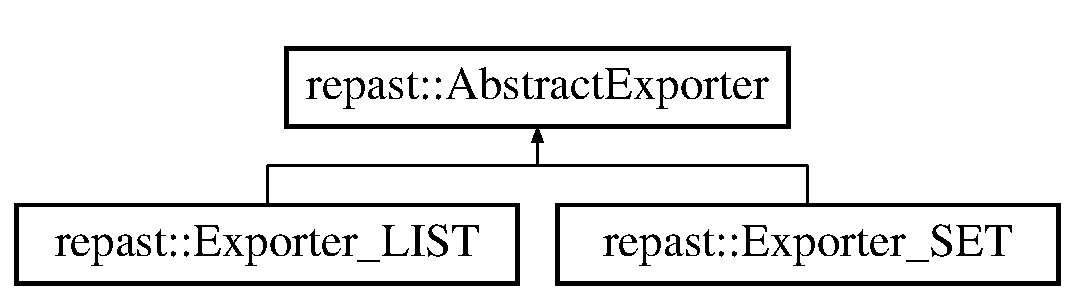
\includegraphics[height=2.000000cm]{classrepast_1_1_abstract_exporter}
\end{center}
\end{figure}
\subsection*{Public Types}
\begin{DoxyCompactItemize}
\item 
\hypertarget{classrepast_1_1_abstract_exporter_a128bcef08654b7749e5fc3d5fc4529ec}{typedef std\-::map$<$ int, \\*
std\-::set$<$ \hyperlink{classrepast_1_1_agent_status}{Agent\-Status} $>$ $>$ {\bfseries Status\-Map}}\label{classrepast_1_1_abstract_exporter_a128bcef08654b7749e5fc3d5fc4529ec}

\end{DoxyCompactItemize}
\subsection*{Public Member Functions}
\begin{DoxyCompactItemize}
\item 
\hypertarget{classrepast_1_1_abstract_exporter_aaf345aa59918904df1847a432f600fba}{virtual void \hyperlink{classrepast_1_1_abstract_exporter_aaf345aa59918904df1847a432f600fba}{register\-Incoming\-Requests} (std\-::vector$<$ \hyperlink{classrepast_1_1_agent_request}{Agent\-Request} $>$ \&requests)=0}\label{classrepast_1_1_abstract_exporter_aaf345aa59918904df1847a432f600fba}

\begin{DoxyCompactList}\small\item\em Makes a record of the data receives (in the form of a vector of Agent\-Requests) so that the agents' data can be sent to the requesting processes. \end{DoxyCompactList}\item 
virtual void \hyperlink{classrepast_1_1_abstract_exporter_a6f75977191b82e5b0c7fc574a9fd4aa1}{incorporate\-Agent\-Exporter\-Info} (std\-::map$<$ int, \hyperlink{classrepast_1_1_agent_request}{Agent\-Request} $\ast$ $>$ info)
\begin{DoxyCompactList}\small\item\em The set of information received here comprises the information that some other process was using to export information about agents that are now being moved to this process. \end{DoxyCompactList}\item 
\hypertarget{classrepast_1_1_abstract_exporter_af3aae158eb37f412c3cb64b7e3be6821}{virtual void \hyperlink{classrepast_1_1_abstract_exporter_af3aae158eb37f412c3cb64b7e3be6821}{agent\-Removed} (const \hyperlink{classrepast_1_1_agent_id}{Agent\-Id} \&id)}\label{classrepast_1_1_abstract_exporter_af3aae158eb37f412c3cb64b7e3be6821}

\begin{DoxyCompactList}\small\item\em 1) Removes the agent export information from this process 2) Updates the outgoing status change buffer to include the status change for this agent to all procs to which this agent was being exported (except if one of these was the proc to which the agent is now moving; this is omitted) \end{DoxyCompactList}\item 
\hypertarget{classrepast_1_1_abstract_exporter_a829612ffd0827dd1120f7dc26f905c36}{virtual void \hyperlink{classrepast_1_1_abstract_exporter_a829612ffd0827dd1120f7dc26f905c36}{agent\-Moved} (const \hyperlink{classrepast_1_1_agent_id}{Agent\-Id} \&id, int process)}\label{classrepast_1_1_abstract_exporter_a829612ffd0827dd1120f7dc26f905c36}

\begin{DoxyCompactList}\small\item\em 1) Removes the agent export information from this process 2) Places a copy of the agent export information into the outgoing buffer 3) Updates the outgoing status change buffer to include the status change for this agent to all procs to which this agent was being exported (except if one of these was the proc to which the agent is now moving; this is omitted) \end{DoxyCompactList}\item 
\hypertarget{classrepast_1_1_abstract_exporter_a4f43a562a4f86fb1e4f4dde47508347a}{virtual const std\-::set$<$ int $>$ \& \hyperlink{classrepast_1_1_abstract_exporter_a4f43a562a4f86fb1e4f4dde47508347a}{get\-Processes\-Exported\-To} ()}\label{classrepast_1_1_abstract_exporter_a4f43a562a4f86fb1e4f4dde47508347a}

\begin{DoxyCompactList}\small\item\em Gets the list of processes this exporter is sending information to. \end{DoxyCompactList}\item 
\hypertarget{classrepast_1_1_abstract_exporter_af63857911d4eb8a59a207daf659c047c}{Agent\-Exporter\-Info $\ast$ \hyperlink{classrepast_1_1_abstract_exporter_af63857911d4eb8a59a207daf659c047c}{get\-Agent\-Export\-Info} (int dest\-Proc)}\label{classrepast_1_1_abstract_exporter_af63857911d4eb8a59a207daf659c047c}

\begin{DoxyCompactList}\small\item\em Gets the export information that has been placed into the 'outgoing agent export information' buffer because agents that were being exported are being sent to a new process, for the specified process. \end{DoxyCompactList}\item 
\hypertarget{classrepast_1_1_abstract_exporter_a6e5c166941bf27d1dfbc6ce9162c327f}{const Status\-Map $\ast$ \hyperlink{classrepast_1_1_abstract_exporter_a6e5c166941bf27d1dfbc6ce9162c327f}{get\-Outgoing\-Status\-Changes} ()}\label{classrepast_1_1_abstract_exporter_a6e5c166941bf27d1dfbc6ce9162c327f}

\begin{DoxyCompactList}\small\item\em Gets the set of status changes for the exported agents. \end{DoxyCompactList}\item 
\hypertarget{classrepast_1_1_abstract_exporter_aaed51e6be3878577e7e226a810d1d8c2}{void \hyperlink{classrepast_1_1_abstract_exporter_aaed51e6be3878577e7e226a810d1d8c2}{clear\-Agent\-Export\-Info} ()}\label{classrepast_1_1_abstract_exporter_aaed51e6be3878577e7e226a810d1d8c2}

\begin{DoxyCompactList}\small\item\em Clears the outgoing agent export information buffer; should be called after the information is sent. \end{DoxyCompactList}\item 
\hypertarget{classrepast_1_1_abstract_exporter_a4a708fff42c4bf1dfb838de5703a6e9a}{void \hyperlink{classrepast_1_1_abstract_exporter_a4a708fff42c4bf1dfb838de5703a6e9a}{clear\-Status\-Map} ()}\label{classrepast_1_1_abstract_exporter_a4a708fff42c4bf1dfb838de5703a6e9a}

\begin{DoxyCompactList}\small\item\em Clears the outgoing status information buffer; should be called after the information is sent. \end{DoxyCompactList}\item 
\hypertarget{classrepast_1_1_abstract_exporter_a019c347c149ee82688ff94323eb67818}{virtual const std\-::map$<$ int, \\*
\hyperlink{classrepast_1_1_agent_request}{Agent\-Request} $>$ \& \hyperlink{classrepast_1_1_abstract_exporter_a019c347c149ee82688ff94323eb67818}{get\-Agents\-To\-Export} ()}\label{classrepast_1_1_abstract_exporter_a019c347c149ee82688ff94323eb67818}

\begin{DoxyCompactList}\small\item\em Gets the list of agents being exported by this exported, as a map by ints representing the processes to which information will be sent. \end{DoxyCompactList}\item 
\hypertarget{classrepast_1_1_abstract_exporter_a02dbd775ca06cc90edc3c8a4834f116a}{{\bfseries Abstract\-Exporter} (Status\-Map $\ast$outgoing\-Status\-Map, \hyperlink{classrepast_1_1_agent_exporter_data}{Agent\-Exporter\-Data} $\ast$outgoing\-Agent\-Exporter\-Info)}\label{classrepast_1_1_abstract_exporter_a02dbd775ca06cc90edc3c8a4834f116a}

\item 
\hypertarget{classrepast_1_1_abstract_exporter_aee45d6557fa45a2690889dbe309d36e6}{virtual std\-::string \hyperlink{classrepast_1_1_abstract_exporter_aee45d6557fa45a2690889dbe309d36e6}{get\-Report} ()=0}\label{classrepast_1_1_abstract_exporter_aee45d6557fa45a2690889dbe309d36e6}

\begin{DoxyCompactList}\small\item\em Gets a printable report of the state of this object. \end{DoxyCompactList}\item 
\hypertarget{classrepast_1_1_abstract_exporter_a5db82162c555e9e223e6083665266163}{virtual void {\bfseries clear} ()}\label{classrepast_1_1_abstract_exporter_a5db82162c555e9e223e6083665266163}

\item 
\hypertarget{classrepast_1_1_abstract_exporter_adebe9add519210ab436c3fae09899cc7}{virtual void {\bfseries clear\-Export\-To\-Specific\-Proc} (int rank)}\label{classrepast_1_1_abstract_exporter_adebe9add519210ab436c3fae09899cc7}

\end{DoxyCompactItemize}
\subsection*{Protected Attributes}
\begin{DoxyCompactItemize}
\item 
\hypertarget{classrepast_1_1_abstract_exporter_ad116dd70f9517119e2d2712beb33adc8}{Status\-Map $\ast$ {\bfseries outgoing\-Status\-Changes}}\label{classrepast_1_1_abstract_exporter_ad116dd70f9517119e2d2712beb33adc8}

\item 
\hypertarget{classrepast_1_1_abstract_exporter_ab3da50572c1fcb852a8676f3deefbf1d}{\hyperlink{classrepast_1_1_agent_exporter_data}{Agent\-Exporter\-Data} $\ast$ {\bfseries outgoing\-Agent\-Exporter\-Information}}\label{classrepast_1_1_abstract_exporter_ab3da50572c1fcb852a8676f3deefbf1d}

\item 
\hypertarget{classrepast_1_1_abstract_exporter_ad61d9e8b964430e130c42d87aad7eab6}{std\-::set$<$ int $>$ {\bfseries processes\-Exported\-To}}\label{classrepast_1_1_abstract_exporter_ad61d9e8b964430e130c42d87aad7eab6}

\item 
\hypertarget{classrepast_1_1_abstract_exporter_aed412358d3bf2742c9445b9b999a81e4}{std\-::map$<$ int, \hyperlink{classrepast_1_1_agent_request}{Agent\-Request} $>$ {\bfseries exported\-Map}}\label{classrepast_1_1_abstract_exporter_aed412358d3bf2742c9445b9b999a81e4}

\end{DoxyCompactItemize}


\subsection{Detailed Description}
Responsible for keeping a list of the agents that have been requested by other processes for which data is to be sent when agents' states are synchronized, and for packaging and sending that data during synchronization. 

It is also responsible for exchanging this 'export' information when any of the agents that it is exporting are being moved to other processes; when an agent moves, its new home process must be able to assume the same export duties that its original process was performing. 

\subsection{Member Function Documentation}
\hypertarget{classrepast_1_1_abstract_exporter_a6f75977191b82e5b0c7fc574a9fd4aa1}{\index{repast\-::\-Abstract\-Exporter@{repast\-::\-Abstract\-Exporter}!incorporate\-Agent\-Exporter\-Info@{incorporate\-Agent\-Exporter\-Info}}
\index{incorporate\-Agent\-Exporter\-Info@{incorporate\-Agent\-Exporter\-Info}!repast::AbstractExporter@{repast\-::\-Abstract\-Exporter}}
\subsubsection[{incorporate\-Agent\-Exporter\-Info}]{\setlength{\rightskip}{0pt plus 5cm}void Abstract\-Exporter\-::incorporate\-Agent\-Exporter\-Info (
\begin{DoxyParamCaption}
\item[{std\-::map$<$ int, {\bf Agent\-Request} $\ast$ $>$}]{info}
\end{DoxyParamCaption}
)\hspace{0.3cm}{\ttfamily [virtual]}}}\label{classrepast_1_1_abstract_exporter_a6f75977191b82e5b0c7fc574a9fd4aa1}


The set of information received here comprises the information that some other process was using to export information about agents that are now being moved to this process. 

This method takes that information and incorporates it into this exporter, so that this exporter can now export the agents' information to the processes that have requested it. 

The documentation for this class was generated from the following files\-:\begin{DoxyCompactItemize}
\item 
repast\-\_\-hpc/Agent\-Importer\-Exporter.\-h\item 
repast\-\_\-hpc/Agent\-Importer\-Exporter.\-cpp\end{DoxyCompactItemize}

\hypertarget{classrepast_1_1_abstract_importer}{\section{repast\-:\-:Abstract\-Importer Class Reference}
\label{classrepast_1_1_abstract_importer}\index{repast\-::\-Abstract\-Importer@{repast\-::\-Abstract\-Importer}}
}


This class manages importing agent information; primarily this means constructing the appropriate mpi receives when agent information is to be exchanged.  




{\ttfamily \#include $<$Agent\-Importer\-Exporter.\-h$>$}

Inheritance diagram for repast\-:\-:Abstract\-Importer\-:\begin{figure}[H]
\begin{center}
\leavevmode
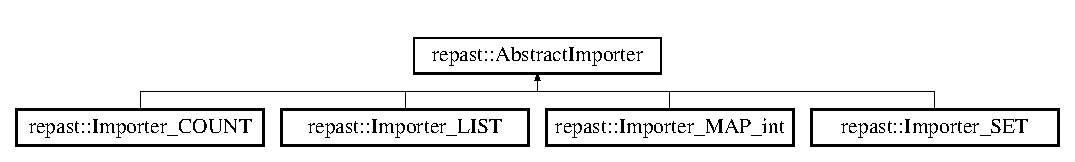
\includegraphics[height=1.728395cm]{classrepast_1_1_abstract_importer}
\end{center}
\end{figure}
\subsection*{Public Member Functions}
\begin{DoxyCompactItemize}
\item 
\hypertarget{classrepast_1_1_abstract_importer_ac32aaff9cd5bc7d300921bdc077b617c}{virtual const std\-::set$<$ int $>$ \& \hyperlink{classrepast_1_1_abstract_importer_ac32aaff9cd5bc7d300921bdc077b617c}{get\-Exporting\-Processes} ()}\label{classrepast_1_1_abstract_importer_ac32aaff9cd5bc7d300921bdc077b617c}

\begin{DoxyCompactList}\small\item\em Gets a const reference to the set of ints representing the processes that are sending this process agent information. \end{DoxyCompactList}\item 
virtual void \hyperlink{classrepast_1_1_abstract_importer_a1353cfde773ce5b3e7011571aff1f823}{register\-Outgoing\-Requests} (\hyperlink{classrepast_1_1_agent_request}{Agent\-Request} \&req)=0
\begin{DoxyCompactList}\small\item\em Given an agent request (including requests for agents on multiple other processes), makes a record of the agents that are being requested by this process and will therefore be received from other processes. \end{DoxyCompactList}\item 
\hypertarget{classrepast_1_1_abstract_importer_a7fc3bf6bb7ee568fb93f03c296c3ea0e}{virtual void \hyperlink{classrepast_1_1_abstract_importer_a7fc3bf6bb7ee568fb93f03c296c3ea0e}{imported\-Agent\-Is\-Removed} (const \hyperlink{classrepast_1_1_agent_id}{Agent\-Id} \&id)=0}\label{classrepast_1_1_abstract_importer_a7fc3bf6bb7ee568fb93f03c296c3ea0e}

\begin{DoxyCompactList}\small\item\em Notifies this importer that the agent that it (presumably) has been importing has been removed from the simulation on its home process, and the information for that agent will no longer be sent. \end{DoxyCompactList}\item 
\hypertarget{classrepast_1_1_abstract_importer_aba04688b4375bcc80278c4ec7ffdceb1}{virtual void \hyperlink{classrepast_1_1_abstract_importer_aba04688b4375bcc80278c4ec7ffdceb1}{imported\-Agent\-Is\-Moved} (const \hyperlink{classrepast_1_1_agent_id}{Agent\-Id} \&id, int new\-Process)=0}\label{classrepast_1_1_abstract_importer_aba04688b4375bcc80278c4ec7ffdceb1}

\begin{DoxyCompactList}\small\item\em Notifies this importer that the agent that it (presumably) has been importing from another process has been moved; its information will now be received from its new home process (unless the agent was moved to this process) \end{DoxyCompactList}\item 
\hypertarget{classrepast_1_1_abstract_importer_a4797219171a2399745cab0a6e576c353}{void \hyperlink{classrepast_1_1_abstract_importer_a4797219171a2399745cab0a6e576c353}{imported\-Agent\-Is\-Now\-Local} (const \hyperlink{classrepast_1_1_agent_id}{Agent\-Id} \&id)}\label{classrepast_1_1_abstract_importer_a4797219171a2399745cab0a6e576c353}

\begin{DoxyCompactList}\small\item\em Some semantic sugar; operationally this is the same as 'imported\-Agent\-Is\-Removed'. \end{DoxyCompactList}\item 
\hypertarget{classrepast_1_1_abstract_importer_a88f4cf004854b5586832e94346fd6f09}{virtual std\-::string \hyperlink{classrepast_1_1_abstract_importer_a88f4cf004854b5586832e94346fd6f09}{get\-Report} ()=0}\label{classrepast_1_1_abstract_importer_a88f4cf004854b5586832e94346fd6f09}

\begin{DoxyCompactList}\small\item\em Get a printable indication of the data in this object. \end{DoxyCompactList}\item 
\hypertarget{classrepast_1_1_abstract_importer_a108ac85357128d13cab863d8d63c74d4}{virtual void {\bfseries get\-Set\-Of\-Agents\-Being\-Imported} (std\-::set$<$ \hyperlink{classrepast_1_1_agent_id}{Agent\-Id} $>$ \&set)=0}\label{classrepast_1_1_abstract_importer_a108ac85357128d13cab863d8d63c74d4}

\item 
\hypertarget{classrepast_1_1_abstract_importer_ad4effa8810c5bbe3f584d06283293a51}{virtual void {\bfseries clear} ()}\label{classrepast_1_1_abstract_importer_ad4effa8810c5bbe3f584d06283293a51}

\end{DoxyCompactItemize}
\subsection*{Protected Attributes}
\begin{DoxyCompactItemize}
\item 
\hypertarget{classrepast_1_1_abstract_importer_a80a457a09ccb2c2b0ac589d2fdaa4e81}{std\-::set$<$ int $>$ {\bfseries exporting\-Processes}}\label{classrepast_1_1_abstract_importer_a80a457a09ccb2c2b0ac589d2fdaa4e81}

\end{DoxyCompactItemize}


\subsection{Detailed Description}
This class manages importing agent information; primarily this means constructing the appropriate mpi receives when agent information is to be exchanged. 

However, this class can also define specific semantics that can apply to agent requests-\/ what to do in the case that an agent is requested twice, for example. 

\subsection{Member Function Documentation}
\hypertarget{classrepast_1_1_abstract_importer_a1353cfde773ce5b3e7011571aff1f823}{\index{repast\-::\-Abstract\-Importer@{repast\-::\-Abstract\-Importer}!register\-Outgoing\-Requests@{register\-Outgoing\-Requests}}
\index{register\-Outgoing\-Requests@{register\-Outgoing\-Requests}!repast::AbstractImporter@{repast\-::\-Abstract\-Importer}}
\subsubsection[{register\-Outgoing\-Requests}]{\setlength{\rightskip}{0pt plus 5cm}virtual void repast\-::\-Abstract\-Importer\-::register\-Outgoing\-Requests (
\begin{DoxyParamCaption}
\item[{{\bf Agent\-Request} \&}]{req}
\end{DoxyParamCaption}
)\hspace{0.3cm}{\ttfamily [pure virtual]}}}\label{classrepast_1_1_abstract_importer_a1353cfde773ce5b3e7011571aff1f823}


Given an agent request (including requests for agents on multiple other processes), makes a record of the agents that are being requested by this process and will therefore be received from other processes. 

The record must at a minimum indicate which other processes are sending agent information, but may include other information, such as how many times a particular agent has been requested. 

Implemented in \hyperlink{classrepast_1_1_importer___m_a_p__int_aa68061de5fd367ebac5e3b85d184a8e3}{repast\-::\-Importer\-\_\-\-M\-A\-P\-\_\-int}, \hyperlink{classrepast_1_1_importer___s_e_t_a129e0998455430f6036897ab209ef163}{repast\-::\-Importer\-\_\-\-S\-E\-T}, \hyperlink{classrepast_1_1_importer___l_i_s_t_a5be3bf4dda0a23db4727882511e2e224}{repast\-::\-Importer\-\_\-\-L\-I\-S\-T}, and \hyperlink{classrepast_1_1_importer___c_o_u_n_t_a37a926665920b7674009603f6512b40e}{repast\-::\-Importer\-\_\-\-C\-O\-U\-N\-T}.



The documentation for this class was generated from the following files\-:\begin{DoxyCompactItemize}
\item 
repast\-\_\-hpc/Agent\-Importer\-Exporter.\-h\item 
repast\-\_\-hpc/Agent\-Importer\-Exporter.\-cpp\end{DoxyCompactItemize}

\hypertarget{classrepast_1_1_abstract_importer_exporter}{\section{repast\-:\-:Abstract\-Importer\-Exporter Class Reference}
\label{classrepast_1_1_abstract_importer_exporter}\index{repast\-::\-Abstract\-Importer\-Exporter@{repast\-::\-Abstract\-Importer\-Exporter}}
}


Wraps and Importer and an Exporter so that both use commensurate semantics and all imports and exports are balanced.  




{\ttfamily \#include $<$Agent\-Importer\-Exporter.\-h$>$}

Inheritance diagram for repast\-:\-:Abstract\-Importer\-Exporter\-:\begin{figure}[H]
\begin{center}
\leavevmode
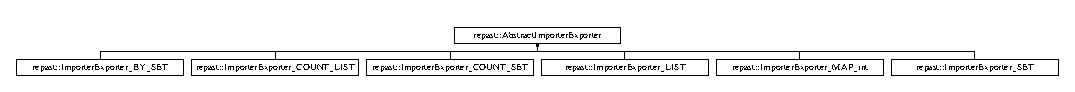
\includegraphics[height=0.787623cm]{classrepast_1_1_abstract_importer_exporter}
\end{center}
\end{figure}
\subsection*{Public Member Functions}
\begin{DoxyCompactItemize}
\item 
\hypertarget{classrepast_1_1_abstract_importer_exporter_ac873303b2cf649afd26ea93b790494a8}{{\bfseries Abstract\-Importer\-Exporter} (\hyperlink{classrepast_1_1_abstract_importer}{Abstract\-Importer} $\ast$i, \hyperlink{classrepast_1_1_abstract_exporter}{Abstract\-Exporter} $\ast$e)}\label{classrepast_1_1_abstract_importer_exporter_ac873303b2cf649afd26ea93b790494a8}

\item 
\hypertarget{classrepast_1_1_abstract_importer_exporter_a6d77b384448820417925f286a9cf21ea}{virtual const std\-::set$<$ int $>$ \& {\bfseries get\-Exporting\-Processes} ()}\label{classrepast_1_1_abstract_importer_exporter_a6d77b384448820417925f286a9cf21ea}

\item 
\hypertarget{classrepast_1_1_abstract_importer_exporter_a599da36e52d78fbabfd3709d9f68a188}{virtual void {\bfseries register\-Outgoing\-Requests} (\hyperlink{classrepast_1_1_agent_request}{Agent\-Request} \&req)}\label{classrepast_1_1_abstract_importer_exporter_a599da36e52d78fbabfd3709d9f68a188}

\item 
\hypertarget{classrepast_1_1_abstract_importer_exporter_a37f4c70de603140adb08b31097cad4f2}{virtual void {\bfseries imported\-Agent\-Is\-Removed} (const \hyperlink{classrepast_1_1_agent_id}{Agent\-Id} \&id)}\label{classrepast_1_1_abstract_importer_exporter_a37f4c70de603140adb08b31097cad4f2}

\item 
\hypertarget{classrepast_1_1_abstract_importer_exporter_a78e60fce871101a398153fa5d8b724f7}{virtual void {\bfseries imported\-Agent\-Is\-Moved} (const \hyperlink{classrepast_1_1_agent_id}{Agent\-Id} \&id, int new\-Process)}\label{classrepast_1_1_abstract_importer_exporter_a78e60fce871101a398153fa5d8b724f7}

\item 
\hypertarget{classrepast_1_1_abstract_importer_exporter_abdbc81ef948b0f332acb99fc4cc9d73a}{virtual void {\bfseries imported\-Agent\-Is\-Now\-Local} (const \hyperlink{classrepast_1_1_agent_id}{Agent\-Id} \&id)}\label{classrepast_1_1_abstract_importer_exporter_abdbc81ef948b0f332acb99fc4cc9d73a}

\item 
\hypertarget{classrepast_1_1_abstract_importer_exporter_a16060c7a93655595503f58570d41f49d}{virtual void {\bfseries get\-Set\-Of\-Agents\-Being\-Imported} (std\-::set$<$ \hyperlink{classrepast_1_1_agent_id}{Agent\-Id} $>$ \&set)}\label{classrepast_1_1_abstract_importer_exporter_a16060c7a93655595503f58570d41f49d}

\item 
\hypertarget{classrepast_1_1_abstract_importer_exporter_a85f8dc96a48418f591745d360c513b5c}{virtual const \\*
Abstract\-Exporter\-::\-Status\-Map $\ast$ {\bfseries get\-Outgoing\-Status\-Changes} ()}\label{classrepast_1_1_abstract_importer_exporter_a85f8dc96a48418f591745d360c513b5c}

\item 
\hypertarget{classrepast_1_1_abstract_importer_exporter_adc150d387a323d81470344d11996b321}{virtual const std\-::set$<$ int $>$ \& {\bfseries get\-Processes\-Exported\-To} ()}\label{classrepast_1_1_abstract_importer_exporter_adc150d387a323d81470344d11996b321}

\item 
\hypertarget{classrepast_1_1_abstract_importer_exporter_af42a1139f782278898edc7ab0250be8c}{virtual void {\bfseries register\-Incoming\-Requests} (std\-::vector$<$ \hyperlink{classrepast_1_1_agent_request}{Agent\-Request} $>$ \&requests)}\label{classrepast_1_1_abstract_importer_exporter_af42a1139f782278898edc7ab0250be8c}

\item 
\hypertarget{classrepast_1_1_abstract_importer_exporter_aaf387c8453d07233e0aa00f128378bd9}{virtual void {\bfseries agent\-Removed} (const \hyperlink{classrepast_1_1_agent_id}{Agent\-Id} \&id)}\label{classrepast_1_1_abstract_importer_exporter_aaf387c8453d07233e0aa00f128378bd9}

\item 
\hypertarget{classrepast_1_1_abstract_importer_exporter_a17611d6966c083c3fe23a44e74284e9a}{virtual void {\bfseries agent\-Moved} (const \hyperlink{classrepast_1_1_agent_id}{Agent\-Id} \&id, int process)}\label{classrepast_1_1_abstract_importer_exporter_a17611d6966c083c3fe23a44e74284e9a}

\item 
\hypertarget{classrepast_1_1_abstract_importer_exporter_ac8dff9fe69a412ed9ff662952f9fc5b7}{virtual void {\bfseries incorporate\-Agent\-Exporter\-Info} (std\-::map$<$ int, \hyperlink{classrepast_1_1_agent_request}{Agent\-Request} $\ast$ $>$ info)}\label{classrepast_1_1_abstract_importer_exporter_ac8dff9fe69a412ed9ff662952f9fc5b7}

\item 
\hypertarget{classrepast_1_1_abstract_importer_exporter_a007e8c17c3fa161f7ad1439074ed56d2}{virtual void {\bfseries clear\-Status\-Map} ()}\label{classrepast_1_1_abstract_importer_exporter_a007e8c17c3fa161f7ad1439074ed56d2}

\item 
\hypertarget{classrepast_1_1_abstract_importer_exporter_a402a82879f25681477af4d3665aa5f6d}{virtual Agent\-Exporter\-Info $\ast$ {\bfseries get\-Agent\-Export\-Info} (int dest\-Proc)}\label{classrepast_1_1_abstract_importer_exporter_a402a82879f25681477af4d3665aa5f6d}

\item 
\hypertarget{classrepast_1_1_abstract_importer_exporter_af83c0409da5354cb6a48641517e174f5}{virtual void {\bfseries clear\-Agent\-Export\-Info} ()}\label{classrepast_1_1_abstract_importer_exporter_af83c0409da5354cb6a48641517e174f5}

\item 
\hypertarget{classrepast_1_1_abstract_importer_exporter_aa88970b511ae80858bb67a9d825a5ba6}{virtual const std\-::map$<$ int, \\*
\hyperlink{classrepast_1_1_agent_request}{Agent\-Request} $>$ \& {\bfseries get\-Agents\-To\-Export} ()}\label{classrepast_1_1_abstract_importer_exporter_aa88970b511ae80858bb67a9d825a5ba6}

\item 
virtual void \hyperlink{classrepast_1_1_abstract_importer_exporter_a545aebe534629acb3061449351da289a}{exchange\-Agent\-Status\-Updates} (boost\-::mpi\-::communicator world, std\-::vector$<$ std\-::vector$<$ \hyperlink{classrepast_1_1_agent_status}{Agent\-Status} $>$ $\ast$ $>$ \&status\-Updates)
\begin{DoxyCompactList}\small\item\em Exchanges the contents of the 'status\-Map' with the destination processes, updating the status (moved or removed) for all agents being exported. \end{DoxyCompactList}\item 
virtual std\-::string \hyperlink{classrepast_1_1_abstract_importer_exporter_a27a52b5ec4ec41e3ed6bf1c8819c25fc}{version} ()=0
\begin{DoxyCompactList}\small\item\em Returns the version of this \hyperlink{classrepast_1_1_abstract_importer_exporter}{Abstract\-Importer\-Exporter}. \end{DoxyCompactList}\item 
\hypertarget{classrepast_1_1_abstract_importer_exporter_ab9cf2ceec7a25942ad964ae426c906c0}{virtual std\-::string \hyperlink{classrepast_1_1_abstract_importer_exporter_ab9cf2ceec7a25942ad964ae426c906c0}{get\-Report} ()}\label{classrepast_1_1_abstract_importer_exporter_ab9cf2ceec7a25942ad964ae426c906c0}

\begin{DoxyCompactList}\small\item\em Gets a printable report of the state of this object. \end{DoxyCompactList}\item 
\hypertarget{classrepast_1_1_abstract_importer_exporter_ab57eba622eb30e4ba582e34ffc824e75}{virtual void {\bfseries clear} ()}\label{classrepast_1_1_abstract_importer_exporter_ab57eba622eb30e4ba582e34ffc824e75}

\item 
\hypertarget{classrepast_1_1_abstract_importer_exporter_a9354b5573205709463f3eedecc764545}{virtual void {\bfseries clear\-Exporter} ()}\label{classrepast_1_1_abstract_importer_exporter_a9354b5573205709463f3eedecc764545}

\item 
\hypertarget{classrepast_1_1_abstract_importer_exporter_ad5166b403fde572938f4785b6609b59d}{virtual void {\bfseries clear\-Export\-To\-Specific\-Proc} (int rank)}\label{classrepast_1_1_abstract_importer_exporter_ad5166b403fde572938f4785b6609b59d}

\end{DoxyCompactItemize}
\subsection*{Protected Attributes}
\begin{DoxyCompactItemize}
\item 
\hypertarget{classrepast_1_1_abstract_importer_exporter_ad987855240b21c39cdfb0f0ffc2b4af1}{\hyperlink{classrepast_1_1_abstract_importer}{Abstract\-Importer} $\ast$ {\bfseries importer}}\label{classrepast_1_1_abstract_importer_exporter_ad987855240b21c39cdfb0f0ffc2b4af1}

\item 
\hypertarget{classrepast_1_1_abstract_importer_exporter_a3090b10b2021c25aeb73c879b0979b75}{\hyperlink{classrepast_1_1_abstract_exporter}{Abstract\-Exporter} $\ast$ {\bfseries exporter}}\label{classrepast_1_1_abstract_importer_exporter_a3090b10b2021c25aeb73c879b0979b75}

\end{DoxyCompactItemize}


\subsection{Detailed Description}
Wraps and Importer and an Exporter so that both use commensurate semantics and all imports and exports are balanced. 

Most methods are pass-\/through to the underlying importer or exporter. 

\subsection{Member Function Documentation}
\hypertarget{classrepast_1_1_abstract_importer_exporter_a545aebe534629acb3061449351da289a}{\index{repast\-::\-Abstract\-Importer\-Exporter@{repast\-::\-Abstract\-Importer\-Exporter}!exchange\-Agent\-Status\-Updates@{exchange\-Agent\-Status\-Updates}}
\index{exchange\-Agent\-Status\-Updates@{exchange\-Agent\-Status\-Updates}!repast::AbstractImporterExporter@{repast\-::\-Abstract\-Importer\-Exporter}}
\subsubsection[{exchange\-Agent\-Status\-Updates}]{\setlength{\rightskip}{0pt plus 5cm}void Abstract\-Importer\-Exporter\-::exchange\-Agent\-Status\-Updates (
\begin{DoxyParamCaption}
\item[{boost\-::mpi\-::communicator}]{world, }
\item[{std\-::vector$<$ std\-::vector$<$ {\bf Agent\-Status} $>$ $\ast$ $>$ \&}]{status\-Updates}
\end{DoxyParamCaption}
)\hspace{0.3cm}{\ttfamily [virtual]}}}\label{classrepast_1_1_abstract_importer_exporter_a545aebe534629acb3061449351da289a}


Exchanges the contents of the 'status\-Map' with the destination processes, updating the status (moved or removed) for all agents being exported. 

Returns this information in the status\-Updates vector. \hypertarget{classrepast_1_1_abstract_importer_exporter_a27a52b5ec4ec41e3ed6bf1c8819c25fc}{\index{repast\-::\-Abstract\-Importer\-Exporter@{repast\-::\-Abstract\-Importer\-Exporter}!version@{version}}
\index{version@{version}!repast::AbstractImporterExporter@{repast\-::\-Abstract\-Importer\-Exporter}}
\subsubsection[{version}]{\setlength{\rightskip}{0pt plus 5cm}virtual std\-::string repast\-::\-Abstract\-Importer\-Exporter\-::version (
\begin{DoxyParamCaption}
{}
\end{DoxyParamCaption}
)\hspace{0.3cm}{\ttfamily [pure virtual]}}}\label{classrepast_1_1_abstract_importer_exporter_a27a52b5ec4ec41e3ed6bf1c8819c25fc}


Returns the version of this \hyperlink{classrepast_1_1_abstract_importer_exporter}{Abstract\-Importer\-Exporter}. 

The version is a string that indicates the semantic version of the importer and the exporter (e.\-g. \char`\"{}\-C\-O\-U\-N\-T\-\_\-\-L\-I\-S\-T\char`\"{}) 

Implemented in \hyperlink{classrepast_1_1_importer_exporter___b_y___s_e_t_a440dc78901d8811ba6046d769df298d9}{repast\-::\-Importer\-Exporter\-\_\-\-B\-Y\-\_\-\-S\-E\-T}, \hyperlink{classrepast_1_1_importer_exporter___m_a_p__int_a801fce0ea8f65aa5b23cc9b1cc9dd818}{repast\-::\-Importer\-Exporter\-\_\-\-M\-A\-P\-\_\-int}, \hyperlink{classrepast_1_1_importer_exporter___s_e_t_a94bcc5a0cb77c6550927663b04410ca2}{repast\-::\-Importer\-Exporter\-\_\-\-S\-E\-T}, \hyperlink{classrepast_1_1_importer_exporter___l_i_s_t_a548c16411acb6e380e9e27139148e294}{repast\-::\-Importer\-Exporter\-\_\-\-L\-I\-S\-T}, \hyperlink{classrepast_1_1_importer_exporter___c_o_u_n_t___s_e_t_a4feec2dc77e01798f1331381198ce3e7}{repast\-::\-Importer\-Exporter\-\_\-\-C\-O\-U\-N\-T\-\_\-\-S\-E\-T}, and \hyperlink{classrepast_1_1_importer_exporter___c_o_u_n_t___l_i_s_t_a576d3dc96aa00bab8a4f0bbe6e64981c}{repast\-::\-Importer\-Exporter\-\_\-\-C\-O\-U\-N\-T\-\_\-\-L\-I\-S\-T}.



The documentation for this class was generated from the following files\-:\begin{DoxyCompactItemize}
\item 
repast\-\_\-hpc/Agent\-Importer\-Exporter.\-h\item 
repast\-\_\-hpc/Agent\-Importer\-Exporter.\-cpp\end{DoxyCompactItemize}

\hypertarget{classrepast_1_1_agent}{\section{repast\-:\-:Agent Class Reference}
\label{classrepast_1_1_agent}\index{repast\-::\-Agent@{repast\-::\-Agent}}
}


Interface for agent classes.  




{\ttfamily \#include $<$Agent\-Id.\-h$>$}

\subsection*{Public Member Functions}
\begin{DoxyCompactItemize}
\item 
virtual \hyperlink{classrepast_1_1_agent_id}{Agent\-Id} \& \hyperlink{classrepast_1_1_agent_ad74523148f3e5df3772bc2a9fd3379d7}{get\-Id} ()=0
\begin{DoxyCompactList}\small\item\em Gets the \hyperlink{classrepast_1_1_agent_id}{Agent\-Id} for this \hyperlink{classrepast_1_1_agent}{Agent}. \end{DoxyCompactList}\item 
virtual const \hyperlink{classrepast_1_1_agent_id}{Agent\-Id} \& \hyperlink{classrepast_1_1_agent_aa091ef26a7a50393d5d3197ea1331eb0}{get\-Id} () const =0
\begin{DoxyCompactList}\small\item\em Gets the \hyperlink{classrepast_1_1_agent_id}{Agent\-Id} for this \hyperlink{classrepast_1_1_agent}{Agent}. \end{DoxyCompactList}\end{DoxyCompactItemize}


\subsection{Detailed Description}
Interface for agent classes. 

\subsection{Member Function Documentation}
\hypertarget{classrepast_1_1_agent_ad74523148f3e5df3772bc2a9fd3379d7}{\index{repast\-::\-Agent@{repast\-::\-Agent}!get\-Id@{get\-Id}}
\index{get\-Id@{get\-Id}!repast::Agent@{repast\-::\-Agent}}
\subsubsection[{get\-Id}]{\setlength{\rightskip}{0pt plus 5cm}virtual {\bf Agent\-Id}\& repast\-::\-Agent\-::get\-Id (
\begin{DoxyParamCaption}
{}
\end{DoxyParamCaption}
)\hspace{0.3cm}{\ttfamily [pure virtual]}}}\label{classrepast_1_1_agent_ad74523148f3e5df3772bc2a9fd3379d7}


Gets the \hyperlink{classrepast_1_1_agent_id}{Agent\-Id} for this \hyperlink{classrepast_1_1_agent}{Agent}. 

\begin{DoxyReturn}{Returns}
the \hyperlink{classrepast_1_1_agent_id}{Agent\-Id} for this \hyperlink{classrepast_1_1_agent}{Agent}. 
\end{DoxyReturn}
\hypertarget{classrepast_1_1_agent_aa091ef26a7a50393d5d3197ea1331eb0}{\index{repast\-::\-Agent@{repast\-::\-Agent}!get\-Id@{get\-Id}}
\index{get\-Id@{get\-Id}!repast::Agent@{repast\-::\-Agent}}
\subsubsection[{get\-Id}]{\setlength{\rightskip}{0pt plus 5cm}virtual const {\bf Agent\-Id}\& repast\-::\-Agent\-::get\-Id (
\begin{DoxyParamCaption}
{}
\end{DoxyParamCaption}
) const\hspace{0.3cm}{\ttfamily [pure virtual]}}}\label{classrepast_1_1_agent_aa091ef26a7a50393d5d3197ea1331eb0}


Gets the \hyperlink{classrepast_1_1_agent_id}{Agent\-Id} for this \hyperlink{classrepast_1_1_agent}{Agent}. 

\begin{DoxyReturn}{Returns}
the \hyperlink{classrepast_1_1_agent_id}{Agent\-Id} for this \hyperlink{classrepast_1_1_agent}{Agent}. 
\end{DoxyReturn}


The documentation for this class was generated from the following file\-:\begin{DoxyCompactItemize}
\item 
repast\-\_\-hpc/Agent\-Id.\-h\end{DoxyCompactItemize}

\hypertarget{classrepast_1_1_agent_exporter_data}{\section{repast\-:\-:Agent\-Exporter\-Data Class Reference}
\label{classrepast_1_1_agent_exporter_data}\index{repast\-::\-Agent\-Exporter\-Data@{repast\-::\-Agent\-Exporter\-Data}}
}


Data structure for exporter data that is to be sent to other processes when the agents being exported are moved.  




{\ttfamily \#include $<$Agent\-Importer\-Exporter.\-h$>$}

\subsection*{Public Member Functions}
\begin{DoxyCompactItemize}
\item 
\hypertarget{classrepast_1_1_agent_exporter_data_a68c868fec5c36fa93a92a30dffaca831}{void \hyperlink{classrepast_1_1_agent_exporter_data_a68c868fec5c36fa93a92a30dffaca831}{add\-Data} (const \hyperlink{classrepast_1_1_agent_id}{Agent\-Id} \&id, const int dest\-Proc, const int source\-Proc, const int number\-Of\-Copies=1)}\label{classrepast_1_1_agent_exporter_data_a68c868fec5c36fa93a92a30dffaca831}

\begin{DoxyCompactList}\small\item\em Adds an agent I\-D to this list of data that is being exported to a specific processor (dest\-Proc), so that the agent's information will be exported to another processor (source\-Proc). \end{DoxyCompactList}\item 
\hypertarget{classrepast_1_1_agent_exporter_data_a9fdf268329053c764be760549ccdd6d7}{Agent\-Exporter\-Info $\ast$ \hyperlink{classrepast_1_1_agent_exporter_data_a9fdf268329053c764be760549ccdd6d7}{data\-For\-Proc} (int dest\-Proc)}\label{classrepast_1_1_agent_exporter_data_a9fdf268329053c764be760549ccdd6d7}

\begin{DoxyCompactList}\small\item\em Gets the packaged set of information to be sent to a specific processor. \end{DoxyCompactList}\item 
\hypertarget{classrepast_1_1_agent_exporter_data_a4b7e8a7d438345fdb9dc05adc81abbf3}{void \hyperlink{classrepast_1_1_agent_exporter_data_a4b7e8a7d438345fdb9dc05adc81abbf3}{clear} ()}\label{classrepast_1_1_agent_exporter_data_a4b7e8a7d438345fdb9dc05adc81abbf3}

\begin{DoxyCompactList}\small\item\em Clears this data structure. \end{DoxyCompactList}\item 
\hypertarget{classrepast_1_1_agent_exporter_data_a24802b60c1947b1e3d76d027360c7263}{void \hyperlink{classrepast_1_1_agent_exporter_data_a24802b60c1947b1e3d76d027360c7263}{remove\-All\-Data\-For\-Agent} (\hyperlink{classrepast_1_1_agent_id}{Agent\-Id} \&id)}\label{classrepast_1_1_agent_exporter_data_a24802b60c1947b1e3d76d027360c7263}

\begin{DoxyCompactList}\small\item\em Remove all the data for a specific agent; useful when the agent is removed. \end{DoxyCompactList}\item 
void \hyperlink{classrepast_1_1_agent_exporter_data_a6b3ec37213eb4a2b76d485144e6bcc4c}{select\-Set} (std\-::string set\-Name)
\begin{DoxyCompactList}\small\item\em Specifies that add and retrieve actions are to be performed on the subset of data identified by the given set name. \end{DoxyCompactList}\end{DoxyCompactItemize}


\subsection{Detailed Description}
Data structure for exporter data that is to be sent to other processes when the agents being exported are moved. 

Note that the internal data structure is protected; classes can use this data without knowing its actual internal structure. 

\subsection{Member Function Documentation}
\hypertarget{classrepast_1_1_agent_exporter_data_a6b3ec37213eb4a2b76d485144e6bcc4c}{\index{repast\-::\-Agent\-Exporter\-Data@{repast\-::\-Agent\-Exporter\-Data}!select\-Set@{select\-Set}}
\index{select\-Set@{select\-Set}!repast::AgentExporterData@{repast\-::\-Agent\-Exporter\-Data}}
\subsubsection[{select\-Set}]{\setlength{\rightskip}{0pt plus 5cm}void Agent\-Exporter\-Data\-::select\-Set (
\begin{DoxyParamCaption}
\item[{std\-::string}]{set\-Name}
\end{DoxyParamCaption}
)}}\label{classrepast_1_1_agent_exporter_data_a6b3ec37213eb4a2b76d485144e6bcc4c}


Specifies that add and retrieve actions are to be performed on the subset of data identified by the given set name. 

(Does not affect 'clear' or 'remove\-All\-Data\-For\-Agent') 

The documentation for this class was generated from the following files\-:\begin{DoxyCompactItemize}
\item 
repast\-\_\-hpc/Agent\-Importer\-Exporter.\-h\item 
repast\-\_\-hpc/Agent\-Importer\-Exporter.\-cpp\end{DoxyCompactItemize}

\hypertarget{structrepast_1_1_agent_from_grid_point}{\section{repast\-:\-:Agent\-From\-Grid\-Point$<$ T, G\-P\-Type $>$ Struct Template Reference}
\label{structrepast_1_1_agent_from_grid_point}\index{repast\-::\-Agent\-From\-Grid\-Point$<$ T, G\-P\-Type $>$@{repast\-::\-Agent\-From\-Grid\-Point$<$ T, G\-P\-Type $>$}}
}


Unary function used in the transform\-\_\-iterator that allows context iterators to return the agent maps values.  




{\ttfamily \#include $<$Base\-Grid.\-h$>$}

Inheritance diagram for repast\-:\-:Agent\-From\-Grid\-Point$<$ T, G\-P\-Type $>$\-:\begin{figure}[H]
\begin{center}
\leavevmode
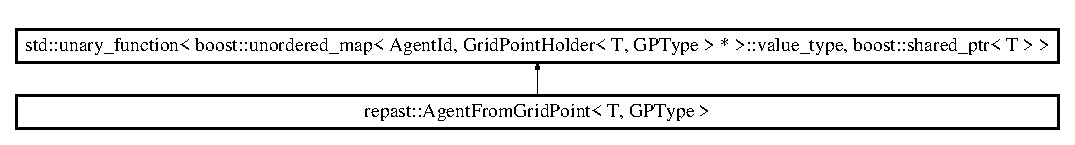
\includegraphics[height=1.505376cm]{structrepast_1_1_agent_from_grid_point}
\end{center}
\end{figure}
\subsection*{Public Member Functions}
\begin{DoxyCompactItemize}
\item 
\hypertarget{structrepast_1_1_agent_from_grid_point_a6ac944644e16ab7ccfb47c0a1acbadae}{boost\-::shared\-\_\-ptr$<$ T $>$ {\bfseries operator()} (const typename boost\-::unordered\-\_\-map$<$ \hyperlink{classrepast_1_1_agent_id}{Agent\-Id}, \hyperlink{structrepast_1_1_grid_point_holder}{Grid\-Point\-Holder}$<$ T, G\-P\-Type $>$ $\ast$ $>$\-::value\-\_\-type \&value) const }\label{structrepast_1_1_agent_from_grid_point_a6ac944644e16ab7ccfb47c0a1acbadae}

\end{DoxyCompactItemize}


\subsection{Detailed Description}
\subsubsection*{template$<$typename T, typename G\-P\-Type$>$struct repast\-::\-Agent\-From\-Grid\-Point$<$ T, G\-P\-Type $>$}

Unary function used in the transform\-\_\-iterator that allows context iterators to return the agent maps values. 

The documentation for this struct was generated from the following file\-:\begin{DoxyCompactItemize}
\item 
repast\-\_\-hpc/Base\-Grid.\-h\end{DoxyCompactItemize}

\hypertarget{structrepast_1_1_agent_hash_id}{\section{repast\-:\-:Agent\-Hash\-Id$<$ Agent\-Type $>$ Struct Template Reference}
\label{structrepast_1_1_agent_hash_id}\index{repast\-::\-Agent\-Hash\-Id$<$ Agent\-Type $>$@{repast\-::\-Agent\-Hash\-Id$<$ Agent\-Type $>$}}
}


operator() implementation that returns the hashcode of an agent via its \hyperlink{classrepast_1_1_agent_id}{Agent\-Id}.  




{\ttfamily \#include $<$Agent\-Id.\-h$>$}

\subsection*{Public Member Functions}
\begin{DoxyCompactItemize}
\item 
\hypertarget{structrepast_1_1_agent_hash_id_afff516755fcf498463f6e7817309851b}{std\-::size\-\_\-t {\bfseries operator()} (const Agent\-Type $\ast$agent) const }\label{structrepast_1_1_agent_hash_id_afff516755fcf498463f6e7817309851b}

\end{DoxyCompactItemize}


\subsection{Detailed Description}
\subsubsection*{template$<$typename Agent\-Type$>$struct repast\-::\-Agent\-Hash\-Id$<$ Agent\-Type $>$}

operator() implementation that returns the hashcode of an agent via its \hyperlink{classrepast_1_1_agent_id}{Agent\-Id}. 

The documentation for this struct was generated from the following file\-:\begin{DoxyCompactItemize}
\item 
repast\-\_\-hpc/Agent\-Id.\-h\end{DoxyCompactItemize}

\hypertarget{classrepast_1_1_agent_id}{\section{repast\-:\-:Agent\-Id Class Reference}
\label{classrepast_1_1_agent_id}\index{repast\-::\-Agent\-Id@{repast\-::\-Agent\-Id}}
}


\hyperlink{classrepast_1_1_agent}{Agent} identity information.  




{\ttfamily \#include $<$Agent\-Id.\-h$>$}

\subsection*{Public Member Functions}
\begin{DoxyCompactItemize}
\item 
\hypertarget{classrepast_1_1_agent_id_ad1da5259ce0bfa4b99f0adea5646ff78}{\hyperlink{classrepast_1_1_agent_id_ad1da5259ce0bfa4b99f0adea5646ff78}{Agent\-Id} ()}\label{classrepast_1_1_agent_id_ad1da5259ce0bfa4b99f0adea5646ff78}

\begin{DoxyCompactList}\small\item\em No-\/arg constructor necessary for serialization. \end{DoxyCompactList}\item 
\hyperlink{classrepast_1_1_agent_id_aedbcc79ba8794ec1d0e7cfb3e7bee83d}{Agent\-Id} (int \hyperlink{classrepast_1_1_agent_id_af8482957f7cc22c0b79b7c62680af219}{id}, int start\-Proc, int \hyperlink{classrepast_1_1_agent_id_a2e28383a437cf176a596783288227e28}{agent\-Type}, int current\-Proc=-\/1)
\begin{DoxyCompactList}\small\item\em Creates an \hyperlink{classrepast_1_1_agent_id}{Agent\-Id}. \end{DoxyCompactList}\item 
int \hyperlink{classrepast_1_1_agent_id_af8482957f7cc22c0b79b7c62680af219}{id} () const 
\begin{DoxyCompactList}\small\item\em Gets the id component of this \hyperlink{classrepast_1_1_agent_id}{Agent\-Id}. \end{DoxyCompactList}\item 
int \hyperlink{classrepast_1_1_agent_id_a8f085b7feffaa55fb958f6b78a76ec43}{starting\-Rank} () const 
\begin{DoxyCompactList}\small\item\em Gets the starting rank component of this \hyperlink{classrepast_1_1_agent_id}{Agent\-Id}. \end{DoxyCompactList}\item 
int \hyperlink{classrepast_1_1_agent_id_a2e28383a437cf176a596783288227e28}{agent\-Type} () const 
\begin{DoxyCompactList}\small\item\em Gets the agent type component of this \hyperlink{classrepast_1_1_agent_id}{Agent\-Id}. \end{DoxyCompactList}\item 
int \hyperlink{classrepast_1_1_agent_id_a2cd64629db02df00ff9718b99f42059f}{current\-Rank} () const 
\begin{DoxyCompactList}\small\item\em Gets the current process rank of this \hyperlink{classrepast_1_1_agent_id}{Agent\-Id}. \end{DoxyCompactList}\item 
void \hyperlink{classrepast_1_1_agent_id_ae55db02b1adb2bf1906fb3356bbc4b21}{current\-Rank} (int val)
\begin{DoxyCompactList}\small\item\em Sets the current process rank of this \hyperlink{classrepast_1_1_agent_id}{Agent\-Id}. \end{DoxyCompactList}\item 
std\-::size\-\_\-t \hyperlink{classrepast_1_1_agent_id_adaf9d5613b079105f0973f7a4eecd86d}{hashcode} () const 
\begin{DoxyCompactList}\small\item\em Gets the hashcode for this \hyperlink{classrepast_1_1_agent_id}{Agent\-Id}. \end{DoxyCompactList}\end{DoxyCompactItemize}
\subsection*{Friends}
\begin{DoxyCompactItemize}
\item 
\hypertarget{classrepast_1_1_agent_id_ac98d07dd8f7b70e16ccb9a01abf56b9c}{class {\bfseries boost\-::serialization\-::access}}\label{classrepast_1_1_agent_id_ac98d07dd8f7b70e16ccb9a01abf56b9c}

\item 
\hypertarget{classrepast_1_1_agent_id_a99514e02ab7b8141d3997fe15d337e98}{std\-::ostream \& \hyperlink{classrepast_1_1_agent_id_a99514e02ab7b8141d3997fe15d337e98}{operator$<$$<$} (std\-::ostream \&os, const \hyperlink{classrepast_1_1_agent_id}{Agent\-Id} \&\hyperlink{classrepast_1_1_agent_id_af8482957f7cc22c0b79b7c62680af219}{id})}\label{classrepast_1_1_agent_id_a99514e02ab7b8141d3997fe15d337e98}

\begin{DoxyCompactList}\small\item\em Writes the agent id to the ostream. \end{DoxyCompactList}\item 
\hypertarget{classrepast_1_1_agent_id_a82148a933e439e1ec53d491438beeb6a}{bool \hyperlink{classrepast_1_1_agent_id_a82148a933e439e1ec53d491438beeb6a}{operator==} (const \hyperlink{classrepast_1_1_agent_id}{Agent\-Id} \&one, const \hyperlink{classrepast_1_1_agent_id}{Agent\-Id} \&two)}\label{classrepast_1_1_agent_id_a82148a933e439e1ec53d491438beeb6a}

\begin{DoxyCompactList}\small\item\em Equality operator. \end{DoxyCompactList}\item 
\hypertarget{classrepast_1_1_agent_id_a96354ea883cef44bf168f04f38d197a1}{bool \hyperlink{classrepast_1_1_agent_id_a96354ea883cef44bf168f04f38d197a1}{operator$<$} (const \hyperlink{classrepast_1_1_agent_id}{Agent\-Id} \&one, const \hyperlink{classrepast_1_1_agent_id}{Agent\-Id} \&two)}\label{classrepast_1_1_agent_id_a96354ea883cef44bf168f04f38d197a1}

\begin{DoxyCompactList}\small\item\em A comparison operator for use with std\-::set. \end{DoxyCompactList}\end{DoxyCompactItemize}


\subsection{Detailed Description}
\hyperlink{classrepast_1_1_agent}{Agent} identity information. 

An \hyperlink{classrepast_1_1_agent}{Agent} I\-D consists of four values\-: 1) a numerical identifier; 2) the process on which the agent was created; 3) a numerical identifier that indicates the agent's type (in simulation semantic terms, not a software object type); and 4) the process on which the agent is a local agent. Each agent should be uniquely identified by an \hyperlink{classrepast_1_1_agent_id}{Agent\-Id} using the first three of the four values, which should be immutable. The fourth value can change throughout the simulation. 

\subsection{Constructor \& Destructor Documentation}
\hypertarget{classrepast_1_1_agent_id_aedbcc79ba8794ec1d0e7cfb3e7bee83d}{\index{repast\-::\-Agent\-Id@{repast\-::\-Agent\-Id}!Agent\-Id@{Agent\-Id}}
\index{Agent\-Id@{Agent\-Id}!repast::AgentId@{repast\-::\-Agent\-Id}}
\subsubsection[{Agent\-Id}]{\setlength{\rightskip}{0pt plus 5cm}repast\-::\-Agent\-Id\-::\-Agent\-Id (
\begin{DoxyParamCaption}
\item[{int}]{id, }
\item[{int}]{start\-Proc, }
\item[{int}]{agent\-Type, }
\item[{int}]{current\-Proc = {\ttfamily -\/1}}
\end{DoxyParamCaption}
)}}\label{classrepast_1_1_agent_id_aedbcc79ba8794ec1d0e7cfb3e7bee83d}


Creates an \hyperlink{classrepast_1_1_agent_id}{Agent\-Id}. 

The combination of the first three parameters should uniquely identify the agent.


\begin{DoxyParams}{Parameters}
{\em id} & the agent's id \\
\hline
{\em start\-Proc} & the rank of the agent's starting process \\
\hline
{\em agent\-Type} & the agent's type (user defined) \\
\hline
{\em current\-Proc} & the rank where the agent is a local agent \\
\hline
\end{DoxyParams}


\subsection{Member Function Documentation}
\hypertarget{classrepast_1_1_agent_id_a2e28383a437cf176a596783288227e28}{\index{repast\-::\-Agent\-Id@{repast\-::\-Agent\-Id}!agent\-Type@{agent\-Type}}
\index{agent\-Type@{agent\-Type}!repast::AgentId@{repast\-::\-Agent\-Id}}
\subsubsection[{agent\-Type}]{\setlength{\rightskip}{0pt plus 5cm}int repast\-::\-Agent\-Id\-::agent\-Type (
\begin{DoxyParamCaption}
{}
\end{DoxyParamCaption}
) const\hspace{0.3cm}{\ttfamily [inline]}}}\label{classrepast_1_1_agent_id_a2e28383a437cf176a596783288227e28}


Gets the agent type component of this \hyperlink{classrepast_1_1_agent_id}{Agent\-Id}. 

\begin{DoxyReturn}{Returns}
the agent type component of this \hyperlink{classrepast_1_1_agent_id}{Agent\-Id}. 
\end{DoxyReturn}
\hypertarget{classrepast_1_1_agent_id_a2cd64629db02df00ff9718b99f42059f}{\index{repast\-::\-Agent\-Id@{repast\-::\-Agent\-Id}!current\-Rank@{current\-Rank}}
\index{current\-Rank@{current\-Rank}!repast::AgentId@{repast\-::\-Agent\-Id}}
\subsubsection[{current\-Rank}]{\setlength{\rightskip}{0pt plus 5cm}int repast\-::\-Agent\-Id\-::current\-Rank (
\begin{DoxyParamCaption}
{}
\end{DoxyParamCaption}
) const\hspace{0.3cm}{\ttfamily [inline]}}}\label{classrepast_1_1_agent_id_a2cd64629db02df00ff9718b99f42059f}


Gets the current process rank of this \hyperlink{classrepast_1_1_agent_id}{Agent\-Id}. 

The current rank identifies which process the agent with this \hyperlink{classrepast_1_1_agent_id}{Agent\-Id} is currently on.

\begin{DoxyReturn}{Returns}
the current process rank of this \hyperlink{classrepast_1_1_agent_id}{Agent\-Id}. 
\end{DoxyReturn}
\hypertarget{classrepast_1_1_agent_id_ae55db02b1adb2bf1906fb3356bbc4b21}{\index{repast\-::\-Agent\-Id@{repast\-::\-Agent\-Id}!current\-Rank@{current\-Rank}}
\index{current\-Rank@{current\-Rank}!repast::AgentId@{repast\-::\-Agent\-Id}}
\subsubsection[{current\-Rank}]{\setlength{\rightskip}{0pt plus 5cm}void repast\-::\-Agent\-Id\-::current\-Rank (
\begin{DoxyParamCaption}
\item[{int}]{val}
\end{DoxyParamCaption}
)\hspace{0.3cm}{\ttfamily [inline]}}}\label{classrepast_1_1_agent_id_ae55db02b1adb2bf1906fb3356bbc4b21}


Sets the current process rank of this \hyperlink{classrepast_1_1_agent_id}{Agent\-Id}. 

The current rank identifies which process the agent with this \hyperlink{classrepast_1_1_agent_id}{Agent\-Id} is currently on.


\begin{DoxyParams}{Parameters}
{\em val} & the current process rank \\
\hline
\end{DoxyParams}
\hypertarget{classrepast_1_1_agent_id_adaf9d5613b079105f0973f7a4eecd86d}{\index{repast\-::\-Agent\-Id@{repast\-::\-Agent\-Id}!hashcode@{hashcode}}
\index{hashcode@{hashcode}!repast::AgentId@{repast\-::\-Agent\-Id}}
\subsubsection[{hashcode}]{\setlength{\rightskip}{0pt plus 5cm}std\-::size\-\_\-t repast\-::\-Agent\-Id\-::hashcode (
\begin{DoxyParamCaption}
{}
\end{DoxyParamCaption}
) const\hspace{0.3cm}{\ttfamily [inline]}}}\label{classrepast_1_1_agent_id_adaf9d5613b079105f0973f7a4eecd86d}


Gets the hashcode for this \hyperlink{classrepast_1_1_agent_id}{Agent\-Id}. 

\begin{DoxyReturn}{Returns}
the hashcode for this \hyperlink{classrepast_1_1_agent_id}{Agent\-Id}. 
\end{DoxyReturn}
\hypertarget{classrepast_1_1_agent_id_af8482957f7cc22c0b79b7c62680af219}{\index{repast\-::\-Agent\-Id@{repast\-::\-Agent\-Id}!id@{id}}
\index{id@{id}!repast::AgentId@{repast\-::\-Agent\-Id}}
\subsubsection[{id}]{\setlength{\rightskip}{0pt plus 5cm}int repast\-::\-Agent\-Id\-::id (
\begin{DoxyParamCaption}
{}
\end{DoxyParamCaption}
) const\hspace{0.3cm}{\ttfamily [inline]}}}\label{classrepast_1_1_agent_id_af8482957f7cc22c0b79b7c62680af219}


Gets the id component of this \hyperlink{classrepast_1_1_agent_id}{Agent\-Id}. 

\begin{DoxyReturn}{Returns}
the id component of this \hyperlink{classrepast_1_1_agent_id}{Agent\-Id}. 
\end{DoxyReturn}
\hypertarget{classrepast_1_1_agent_id_a8f085b7feffaa55fb958f6b78a76ec43}{\index{repast\-::\-Agent\-Id@{repast\-::\-Agent\-Id}!starting\-Rank@{starting\-Rank}}
\index{starting\-Rank@{starting\-Rank}!repast::AgentId@{repast\-::\-Agent\-Id}}
\subsubsection[{starting\-Rank}]{\setlength{\rightskip}{0pt plus 5cm}int repast\-::\-Agent\-Id\-::starting\-Rank (
\begin{DoxyParamCaption}
{}
\end{DoxyParamCaption}
) const\hspace{0.3cm}{\ttfamily [inline]}}}\label{classrepast_1_1_agent_id_a8f085b7feffaa55fb958f6b78a76ec43}


Gets the starting rank component of this \hyperlink{classrepast_1_1_agent_id}{Agent\-Id}. 

\begin{DoxyReturn}{Returns}
the starting rank component of this \hyperlink{classrepast_1_1_agent_id}{Agent\-Id}. 
\end{DoxyReturn}


The documentation for this class was generated from the following files\-:\begin{DoxyCompactItemize}
\item 
repast\-\_\-hpc/Agent\-Id.\-h\item 
repast\-\_\-hpc/Agent\-Id.\-cpp\end{DoxyCompactItemize}

\hypertarget{classrepast_1_1_agent_request}{\section{repast\-:\-:Agent\-Request Class Reference}
\label{classrepast_1_1_agent_request}\index{repast\-::\-Agent\-Request@{repast\-::\-Agent\-Request}}
}


Encapsulates a request made by one process for agents in another.  




{\ttfamily \#include $<$Agent\-Request.\-h$>$}

\subsection*{Public Member Functions}
\begin{DoxyCompactItemize}
\item 
\hyperlink{classrepast_1_1_agent_request_a7fcf54013c3f90c22c52fe26b1f2e355}{Agent\-Request} (int \hyperlink{classrepast_1_1_agent_request_afd2499472864d7d8eb2780fd02baf372}{source\-Process})
\begin{DoxyCompactList}\small\item\em Creates an \hyperlink{classrepast_1_1_agent_request}{Agent\-Request} that comes from the specified process. \end{DoxyCompactList}\item 
\hyperlink{classrepast_1_1_agent_request_a1e302fac20c183af00fd12b669f4f973}{Agent\-Request} (int \hyperlink{classrepast_1_1_agent_request_afd2499472864d7d8eb2780fd02baf372}{source\-Process}, int \hyperlink{classrepast_1_1_agent_request_a19abc9909ceeb4870c07b638e19d6672}{target\-Process})
\begin{DoxyCompactList}\small\item\em Creates an \hyperlink{classrepast_1_1_agent_request}{Agent\-Request} made from the source process to the target process. \end{DoxyCompactList}\item 
void \hyperlink{classrepast_1_1_agent_request_a4ac5995bd89cc5fde63ac0aa5bfaafd2}{add\-All} (const \hyperlink{classrepast_1_1_agent_request}{Agent\-Request} \&req)
\begin{DoxyCompactList}\small\item\em Adds all the agent ids (both requests and cancellations) in req to this \hyperlink{classrepast_1_1_agent_request}{Agent\-Request}. \end{DoxyCompactList}\item 
void \hyperlink{classrepast_1_1_agent_request_ac435adefd74246589b3028dc7aeef5a9}{add\-All\-Requests} (const \hyperlink{classrepast_1_1_agent_request}{Agent\-Request} \&req)
\begin{DoxyCompactList}\small\item\em Adds all the agent ids in req to this request, including only the ids that are requests and not those that are cancellations. \end{DoxyCompactList}\item 
void \hyperlink{classrepast_1_1_agent_request_a446efb284f4804f6d0123c71995237ee}{add\-All\-Cancellations} (const \hyperlink{classrepast_1_1_agent_request}{Agent\-Request} \&req)
\begin{DoxyCompactList}\small\item\em Adds all the agent ids in req to this request, including only the ids that are cancellations and not those that are requests. \end{DoxyCompactList}\item 
const std\-::vector$<$ \hyperlink{classrepast_1_1_agent_id}{Agent\-Id} $>$ \& \hyperlink{classrepast_1_1_agent_request_a7961c3fda219def5e403ec610044524e}{requested\-Agents} () const 
\begin{DoxyCompactList}\small\item\em Gets a reference to the vector of requested agents. \end{DoxyCompactList}\item 
const std\-::vector$<$ \hyperlink{classrepast_1_1_agent_id}{Agent\-Id} $>$ \& \hyperlink{classrepast_1_1_agent_request_aeb621d544c5a888b56407b21d1d37259}{cancellations} () const 
\begin{DoxyCompactList}\small\item\em Gets a reference to the vector of cancellations. \end{DoxyCompactList}\item 
bool \hyperlink{classrepast_1_1_agent_request_a2f984bd8eb8e2dc0ef83ad33de0b7785}{remove} (const \hyperlink{classrepast_1_1_agent_id}{Agent\-Id} \&id, bool remove\-All\-Instances=true)
\begin{DoxyCompactList}\small\item\em Removes the specified id from the lists of requested agents, including both requests and cancellations. \end{DoxyCompactList}\item 
bool \hyperlink{classrepast_1_1_agent_request_a6c96d538e1018733866642978a83e509}{remove\-Request} (const \hyperlink{classrepast_1_1_agent_id}{Agent\-Id} \&id, bool remove\-All\-Instances=true)
\begin{DoxyCompactList}\small\item\em Removes the specified id from the list of agent requests; does not affect the list of cancellations. \end{DoxyCompactList}\item 
bool \hyperlink{classrepast_1_1_agent_request_a24c0912e47b149ee3aa24a5c6a5cff1a}{remove\-Cancellation} (const \hyperlink{classrepast_1_1_agent_id}{Agent\-Id} \&id, bool remove\-All\-Instances=true)
\begin{DoxyCompactList}\small\item\em Removes the specified id from the list of agent request cancellations; does not affect the list of requests. \end{DoxyCompactList}\item 
void \hyperlink{classrepast_1_1_agent_request_a3b46d7118e7e9f4bcf2d4c973bb9ceef}{targets} (std\-::set$<$ int $>$ \&targets)
\begin{DoxyCompactList}\small\item\em Puts the targets of all the requests into the set. \end{DoxyCompactList}\item 
void \hyperlink{classrepast_1_1_agent_request_af1bee79d13a5d15af1a00c9509b540ef}{targets\-Of\-Requests} (std\-::set$<$ int $>$ \&\hyperlink{classrepast_1_1_agent_request_a3b46d7118e7e9f4bcf2d4c973bb9ceef}{targets})
\begin{DoxyCompactList}\small\item\em Puts the targets of all the requests into the set, including only the requests and not the cancellations. \end{DoxyCompactList}\item 
void \hyperlink{classrepast_1_1_agent_request_a158490663d112ae0100478ca71de4908}{targets\-Of\-Cancellations} (std\-::set$<$ int $>$ \&\hyperlink{classrepast_1_1_agent_request_a3b46d7118e7e9f4bcf2d4c973bb9ceef}{targets})
\begin{DoxyCompactList}\small\item\em Puts the targets of all the requests into the set, including only the requests and not the cancellations. \end{DoxyCompactList}\item 
void \hyperlink{classrepast_1_1_agent_request_a357e606a76f671ce603e151e3b3759cb}{add\-Request} (const \hyperlink{classrepast_1_1_agent_id}{Agent\-Id} \&id)
\begin{DoxyCompactList}\small\item\em Adds the specified agent to the collection agents being requested. \end{DoxyCompactList}\item 
void \hyperlink{classrepast_1_1_agent_request_a55316e3d48f9be97552701efd9b0bfea}{add\-Cancellation} (const \hyperlink{classrepast_1_1_agent_id}{Agent\-Id} \&id)
\begin{DoxyCompactList}\small\item\em Adds the specified agent to the collection of agents for which a previous request is being cancelled. \end{DoxyCompactList}\item 
int \hyperlink{classrepast_1_1_agent_request_ab3b18ef9714e7c9cccddda1c91de64ac}{request\-Count} () const 
\begin{DoxyCompactList}\small\item\em Gets the number agents requested. \end{DoxyCompactList}\item 
int \hyperlink{classrepast_1_1_agent_request_a3cc36891325c34f23a074a816618fe81}{request\-Count\-Requested} () const 
\begin{DoxyCompactList}\small\item\em Gets the number of agents requested, counting only the requests and not the cancellations. \end{DoxyCompactList}\item 
int \hyperlink{classrepast_1_1_agent_request_a3e842fbe34e47433f51066eed03983b4}{request\-Count\-Cancellations} () const 
\begin{DoxyCompactList}\small\item\em Gets the number of agents requested, counting only the cancellations and not the requests. \end{DoxyCompactList}\item 
bool \hyperlink{classrepast_1_1_agent_request_aa2389d645973a361b97f4e7f5e1a0b86}{contains} (const \hyperlink{classrepast_1_1_agent_id}{Agent\-Id} \&id)
\begin{DoxyCompactList}\small\item\em Returns true if this \hyperlink{classrepast_1_1_agent_request}{Agent\-Request} contains a request for the specified id (either a request or a cancellation), otherwise false. \end{DoxyCompactList}\item 
bool \hyperlink{classrepast_1_1_agent_request_a31aac02439a7b368e92c65acc11f3bb7}{contains\-In\-Requests} (const \hyperlink{classrepast_1_1_agent_id}{Agent\-Id} \&id)
\begin{DoxyCompactList}\small\item\em Returns true if the list of requests contains the specified id (the list of cancellations is ignored) \end{DoxyCompactList}\item 
bool \hyperlink{classrepast_1_1_agent_request_a680ccca02721405863693f29b2e29ced}{contains\-In\-Cancellations} (const \hyperlink{classrepast_1_1_agent_id}{Agent\-Id} \&id)
\begin{DoxyCompactList}\small\item\em Returns true if the list of cancellations contains the specified id (the list of requests is ignored) \end{DoxyCompactList}\item 
int \hyperlink{classrepast_1_1_agent_request_afd2499472864d7d8eb2780fd02baf372}{source\-Process} () const 
\begin{DoxyCompactList}\small\item\em Gets the source process of these requests, that is, the process making the request. \end{DoxyCompactList}\item 
int \hyperlink{classrepast_1_1_agent_request_a19abc9909ceeb4870c07b638e19d6672}{target\-Process} () const 
\begin{DoxyCompactList}\small\item\em If the requested agent ids are all on the same process then target process will identify that process. \end{DoxyCompactList}\end{DoxyCompactItemize}
\subsection*{Friends}
\begin{DoxyCompactItemize}
\item 
\hypertarget{classrepast_1_1_agent_request_ac98d07dd8f7b70e16ccb9a01abf56b9c}{class {\bfseries boost\-::serialization\-::access}}\label{classrepast_1_1_agent_request_ac98d07dd8f7b70e16ccb9a01abf56b9c}

\item 
\hypertarget{classrepast_1_1_agent_request_aa7639ebf76360a6503e77366cc231d8a}{class {\bfseries Importer\-\_\-\-L\-I\-S\-T}}\label{classrepast_1_1_agent_request_aa7639ebf76360a6503e77366cc231d8a}

\item 
\hypertarget{classrepast_1_1_agent_request_a5a13f6efb82ee26ba1a72200d6f2b47e}{class {\bfseries Importer\-\_\-\-S\-E\-T}}\label{classrepast_1_1_agent_request_a5a13f6efb82ee26ba1a72200d6f2b47e}

\item 
\hypertarget{classrepast_1_1_agent_request_af54ef3fa9be752e0bc2e86fc77d58a4c}{class {\bfseries Importer\-\_\-\-M\-A\-P\-\_\-int}}\label{classrepast_1_1_agent_request_af54ef3fa9be752e0bc2e86fc77d58a4c}

\item 
\hypertarget{classrepast_1_1_agent_request_ae9b3dceacb552223daaa71d44018d4b1}{std\-::ostream \& \hyperlink{classrepast_1_1_agent_request_ae9b3dceacb552223daaa71d44018d4b1}{operator$<$$<$} (std\-::ostream \&os, const \hyperlink{classrepast_1_1_agent_request}{Agent\-Request} \&request)}\label{classrepast_1_1_agent_request_ae9b3dceacb552223daaa71d44018d4b1}

\begin{DoxyCompactList}\small\item\em Prints the specified \hyperlink{classrepast_1_1_agent_request}{Agent\-Request} to the specified ostream. \end{DoxyCompactList}\end{DoxyCompactItemize}


\subsection{Detailed Description}
Encapsulates a request made by one process for agents in another. 

Includes a list of requests and a list that represents cancellations of previous requests. 

\subsection{Constructor \& Destructor Documentation}
\hypertarget{classrepast_1_1_agent_request_a7fcf54013c3f90c22c52fe26b1f2e355}{\index{repast\-::\-Agent\-Request@{repast\-::\-Agent\-Request}!Agent\-Request@{Agent\-Request}}
\index{Agent\-Request@{Agent\-Request}!repast::AgentRequest@{repast\-::\-Agent\-Request}}
\subsubsection[{Agent\-Request}]{\setlength{\rightskip}{0pt plus 5cm}repast\-::\-Agent\-Request\-::\-Agent\-Request (
\begin{DoxyParamCaption}
\item[{int}]{source\-Process}
\end{DoxyParamCaption}
)}}\label{classrepast_1_1_agent_request_a7fcf54013c3f90c22c52fe26b1f2e355}


Creates an \hyperlink{classrepast_1_1_agent_request}{Agent\-Request} that comes from the specified process. 


\begin{DoxyParams}{Parameters}
{\em source\-Process} & the rank of the process making the request \\
\hline
\end{DoxyParams}
\hypertarget{classrepast_1_1_agent_request_a1e302fac20c183af00fd12b669f4f973}{\index{repast\-::\-Agent\-Request@{repast\-::\-Agent\-Request}!Agent\-Request@{Agent\-Request}}
\index{Agent\-Request@{Agent\-Request}!repast::AgentRequest@{repast\-::\-Agent\-Request}}
\subsubsection[{Agent\-Request}]{\setlength{\rightskip}{0pt plus 5cm}repast\-::\-Agent\-Request\-::\-Agent\-Request (
\begin{DoxyParamCaption}
\item[{int}]{source\-Process, }
\item[{int}]{target\-Process}
\end{DoxyParamCaption}
)}}\label{classrepast_1_1_agent_request_a1e302fac20c183af00fd12b669f4f973}


Creates an \hyperlink{classrepast_1_1_agent_request}{Agent\-Request} made from the source process to the target process. 

This can be used when all the requested agents reside on the same process (i.\-e. the target process).


\begin{DoxyParams}{Parameters}
{\em source\-Process} & the rank of the source process \\
\hline
{\em target\-Process} & the rank of the target process \\
\hline
\end{DoxyParams}


\subsection{Member Function Documentation}
\hypertarget{classrepast_1_1_agent_request_a4ac5995bd89cc5fde63ac0aa5bfaafd2}{\index{repast\-::\-Agent\-Request@{repast\-::\-Agent\-Request}!add\-All@{add\-All}}
\index{add\-All@{add\-All}!repast::AgentRequest@{repast\-::\-Agent\-Request}}
\subsubsection[{add\-All}]{\setlength{\rightskip}{0pt plus 5cm}void repast\-::\-Agent\-Request\-::add\-All (
\begin{DoxyParamCaption}
\item[{const {\bf Agent\-Request} \&}]{req}
\end{DoxyParamCaption}
)}}\label{classrepast_1_1_agent_request_a4ac5995bd89cc5fde63ac0aa5bfaafd2}


Adds all the agent ids (both requests and cancellations) in req to this \hyperlink{classrepast_1_1_agent_request}{Agent\-Request}. 


\begin{DoxyParams}{Parameters}
{\em req} & the \hyperlink{classrepast_1_1_agent_request}{Agent\-Request} to add all the agent ids from \\
\hline
\end{DoxyParams}
\hypertarget{classrepast_1_1_agent_request_a446efb284f4804f6d0123c71995237ee}{\index{repast\-::\-Agent\-Request@{repast\-::\-Agent\-Request}!add\-All\-Cancellations@{add\-All\-Cancellations}}
\index{add\-All\-Cancellations@{add\-All\-Cancellations}!repast::AgentRequest@{repast\-::\-Agent\-Request}}
\subsubsection[{add\-All\-Cancellations}]{\setlength{\rightskip}{0pt plus 5cm}void repast\-::\-Agent\-Request\-::add\-All\-Cancellations (
\begin{DoxyParamCaption}
\item[{const {\bf Agent\-Request} \&}]{req}
\end{DoxyParamCaption}
)}}\label{classrepast_1_1_agent_request_a446efb284f4804f6d0123c71995237ee}


Adds all the agent ids in req to this request, including only the ids that are cancellations and not those that are requests. 


\begin{DoxyParams}{Parameters}
{\em req} & the \hyperlink{classrepast_1_1_agent_request}{Agent\-Request} to add all the agent ids from \\
\hline
\end{DoxyParams}
\hypertarget{classrepast_1_1_agent_request_ac435adefd74246589b3028dc7aeef5a9}{\index{repast\-::\-Agent\-Request@{repast\-::\-Agent\-Request}!add\-All\-Requests@{add\-All\-Requests}}
\index{add\-All\-Requests@{add\-All\-Requests}!repast::AgentRequest@{repast\-::\-Agent\-Request}}
\subsubsection[{add\-All\-Requests}]{\setlength{\rightskip}{0pt plus 5cm}void repast\-::\-Agent\-Request\-::add\-All\-Requests (
\begin{DoxyParamCaption}
\item[{const {\bf Agent\-Request} \&}]{req}
\end{DoxyParamCaption}
)}}\label{classrepast_1_1_agent_request_ac435adefd74246589b3028dc7aeef5a9}


Adds all the agent ids in req to this request, including only the ids that are requests and not those that are cancellations. 


\begin{DoxyParams}{Parameters}
{\em req} & the \hyperlink{classrepast_1_1_agent_request}{Agent\-Request} to add all the agent ids from \\
\hline
\end{DoxyParams}
\hypertarget{classrepast_1_1_agent_request_a55316e3d48f9be97552701efd9b0bfea}{\index{repast\-::\-Agent\-Request@{repast\-::\-Agent\-Request}!add\-Cancellation@{add\-Cancellation}}
\index{add\-Cancellation@{add\-Cancellation}!repast::AgentRequest@{repast\-::\-Agent\-Request}}
\subsubsection[{add\-Cancellation}]{\setlength{\rightskip}{0pt plus 5cm}void repast\-::\-Agent\-Request\-::add\-Cancellation (
\begin{DoxyParamCaption}
\item[{const {\bf Agent\-Id} \&}]{id}
\end{DoxyParamCaption}
)}}\label{classrepast_1_1_agent_request_a55316e3d48f9be97552701efd9b0bfea}


Adds the specified agent to the collection of agents for which a previous request is being cancelled. 


\begin{DoxyParams}{Parameters}
{\em id} & the \hyperlink{classrepast_1_1_agent_id}{Agent\-Id} of the agent for which the request is being cancelled \\
\hline
\end{DoxyParams}
\hypertarget{classrepast_1_1_agent_request_a357e606a76f671ce603e151e3b3759cb}{\index{repast\-::\-Agent\-Request@{repast\-::\-Agent\-Request}!add\-Request@{add\-Request}}
\index{add\-Request@{add\-Request}!repast::AgentRequest@{repast\-::\-Agent\-Request}}
\subsubsection[{add\-Request}]{\setlength{\rightskip}{0pt plus 5cm}void repast\-::\-Agent\-Request\-::add\-Request (
\begin{DoxyParamCaption}
\item[{const {\bf Agent\-Id} \&}]{id}
\end{DoxyParamCaption}
)}}\label{classrepast_1_1_agent_request_a357e606a76f671ce603e151e3b3759cb}


Adds the specified agent to the collection agents being requested. 


\begin{DoxyParams}{Parameters}
{\em id} & the requested agent \\
\hline
\end{DoxyParams}
\hypertarget{classrepast_1_1_agent_request_aeb621d544c5a888b56407b21d1d37259}{\index{repast\-::\-Agent\-Request@{repast\-::\-Agent\-Request}!cancellations@{cancellations}}
\index{cancellations@{cancellations}!repast::AgentRequest@{repast\-::\-Agent\-Request}}
\subsubsection[{cancellations}]{\setlength{\rightskip}{0pt plus 5cm}const std\-::vector$<${\bf Agent\-Id}$>$\& repast\-::\-Agent\-Request\-::cancellations (
\begin{DoxyParamCaption}
{}
\end{DoxyParamCaption}
) const\hspace{0.3cm}{\ttfamily [inline]}}}\label{classrepast_1_1_agent_request_aeb621d544c5a888b56407b21d1d37259}


Gets a reference to the vector of cancellations. 

\begin{DoxyReturn}{Returns}
a reference to the vector of Agent\-Ids representing cancellations. 
\end{DoxyReturn}
\hypertarget{classrepast_1_1_agent_request_aa2389d645973a361b97f4e7f5e1a0b86}{\index{repast\-::\-Agent\-Request@{repast\-::\-Agent\-Request}!contains@{contains}}
\index{contains@{contains}!repast::AgentRequest@{repast\-::\-Agent\-Request}}
\subsubsection[{contains}]{\setlength{\rightskip}{0pt plus 5cm}bool repast\-::\-Agent\-Request\-::contains (
\begin{DoxyParamCaption}
\item[{const {\bf Agent\-Id} \&}]{id}
\end{DoxyParamCaption}
)}}\label{classrepast_1_1_agent_request_aa2389d645973a361b97f4e7f5e1a0b86}


Returns true if this \hyperlink{classrepast_1_1_agent_request}{Agent\-Request} contains a request for the specified id (either a request or a cancellation), otherwise false. 


\begin{DoxyParams}{Parameters}
{\em id} & the id sought in the lists of requests and cancellations\\
\hline
\end{DoxyParams}
\begin{DoxyReturn}{Returns}
true if either the list of requests or the list of cancellations contains the specified id 
\end{DoxyReturn}
\hypertarget{classrepast_1_1_agent_request_a680ccca02721405863693f29b2e29ced}{\index{repast\-::\-Agent\-Request@{repast\-::\-Agent\-Request}!contains\-In\-Cancellations@{contains\-In\-Cancellations}}
\index{contains\-In\-Cancellations@{contains\-In\-Cancellations}!repast::AgentRequest@{repast\-::\-Agent\-Request}}
\subsubsection[{contains\-In\-Cancellations}]{\setlength{\rightskip}{0pt plus 5cm}bool repast\-::\-Agent\-Request\-::contains\-In\-Cancellations (
\begin{DoxyParamCaption}
\item[{const {\bf Agent\-Id} \&}]{id}
\end{DoxyParamCaption}
)}}\label{classrepast_1_1_agent_request_a680ccca02721405863693f29b2e29ced}


Returns true if the list of cancellations contains the specified id (the list of requests is ignored) 


\begin{DoxyParams}{Parameters}
{\em id} & the \hyperlink{classrepast_1_1_agent_id}{Agent\-Id} sought\\
\hline
\end{DoxyParams}
\begin{DoxyReturn}{Returns}
true if the specified \hyperlink{classrepast_1_1_agent_id}{Agent\-Id} is in the list of cancellations 
\end{DoxyReturn}
\hypertarget{classrepast_1_1_agent_request_a31aac02439a7b368e92c65acc11f3bb7}{\index{repast\-::\-Agent\-Request@{repast\-::\-Agent\-Request}!contains\-In\-Requests@{contains\-In\-Requests}}
\index{contains\-In\-Requests@{contains\-In\-Requests}!repast::AgentRequest@{repast\-::\-Agent\-Request}}
\subsubsection[{contains\-In\-Requests}]{\setlength{\rightskip}{0pt plus 5cm}bool repast\-::\-Agent\-Request\-::contains\-In\-Requests (
\begin{DoxyParamCaption}
\item[{const {\bf Agent\-Id} \&}]{id}
\end{DoxyParamCaption}
)}}\label{classrepast_1_1_agent_request_a31aac02439a7b368e92c65acc11f3bb7}


Returns true if the list of requests contains the specified id (the list of cancellations is ignored) 


\begin{DoxyParams}{Parameters}
{\em id} & the \hyperlink{classrepast_1_1_agent_id}{Agent\-Id} sought\\
\hline
\end{DoxyParams}
\begin{DoxyReturn}{Returns}
true if the specified \hyperlink{classrepast_1_1_agent_id}{Agent\-Id} is in the list of requests 
\end{DoxyReturn}
\hypertarget{classrepast_1_1_agent_request_a2f984bd8eb8e2dc0ef83ad33de0b7785}{\index{repast\-::\-Agent\-Request@{repast\-::\-Agent\-Request}!remove@{remove}}
\index{remove@{remove}!repast::AgentRequest@{repast\-::\-Agent\-Request}}
\subsubsection[{remove}]{\setlength{\rightskip}{0pt plus 5cm}bool repast\-::\-Agent\-Request\-::remove (
\begin{DoxyParamCaption}
\item[{const {\bf Agent\-Id} \&}]{id, }
\item[{bool}]{remove\-All\-Instances = {\ttfamily true}}
\end{DoxyParamCaption}
)}}\label{classrepast_1_1_agent_request_a2f984bd8eb8e2dc0ef83ad33de0b7785}


Removes the specified id from the lists of requested agents, including both requests and cancellations. 


\begin{DoxyParams}{Parameters}
{\em id} & the \hyperlink{classrepast_1_1_agent_id}{Agent\-Id} to be removed \\
\hline
{\em remove\-All\-Instances} & if true (the default), all instances of the \hyperlink{classrepast_1_1_agent_id}{Agent\-Id} are removed; if false, only the first instance found is removed\\
\hline
\end{DoxyParams}
\begin{DoxyReturn}{Returns}
true if the id was found (in either list) and removed, otherwise false. 
\end{DoxyReturn}
\hypertarget{classrepast_1_1_agent_request_a24c0912e47b149ee3aa24a5c6a5cff1a}{\index{repast\-::\-Agent\-Request@{repast\-::\-Agent\-Request}!remove\-Cancellation@{remove\-Cancellation}}
\index{remove\-Cancellation@{remove\-Cancellation}!repast::AgentRequest@{repast\-::\-Agent\-Request}}
\subsubsection[{remove\-Cancellation}]{\setlength{\rightskip}{0pt plus 5cm}bool repast\-::\-Agent\-Request\-::remove\-Cancellation (
\begin{DoxyParamCaption}
\item[{const {\bf Agent\-Id} \&}]{id, }
\item[{bool}]{remove\-All\-Instances = {\ttfamily true}}
\end{DoxyParamCaption}
)}}\label{classrepast_1_1_agent_request_a24c0912e47b149ee3aa24a5c6a5cff1a}


Removes the specified id from the list of agent request cancellations; does not affect the list of requests. 


\begin{DoxyParams}{Parameters}
{\em id} & the \hyperlink{classrepast_1_1_agent_id}{Agent\-Id} to be removed \\
\hline
{\em remove\-All\-Instances} & if true (the default), all instances of the \hyperlink{classrepast_1_1_agent_id}{Agent\-Id} are removed; if false, only the first instance found is removed\\
\hline
\end{DoxyParams}
\begin{DoxyReturn}{Returns}
true if the id was found in the list of cancellations and removed, otherwise false 
\end{DoxyReturn}
\hypertarget{classrepast_1_1_agent_request_a6c96d538e1018733866642978a83e509}{\index{repast\-::\-Agent\-Request@{repast\-::\-Agent\-Request}!remove\-Request@{remove\-Request}}
\index{remove\-Request@{remove\-Request}!repast::AgentRequest@{repast\-::\-Agent\-Request}}
\subsubsection[{remove\-Request}]{\setlength{\rightskip}{0pt plus 5cm}bool repast\-::\-Agent\-Request\-::remove\-Request (
\begin{DoxyParamCaption}
\item[{const {\bf Agent\-Id} \&}]{id, }
\item[{bool}]{remove\-All\-Instances = {\ttfamily true}}
\end{DoxyParamCaption}
)}}\label{classrepast_1_1_agent_request_a6c96d538e1018733866642978a83e509}


Removes the specified id from the list of agent requests; does not affect the list of cancellations. 


\begin{DoxyParams}{Parameters}
{\em id} & the \hyperlink{classrepast_1_1_agent_id}{Agent\-Id} to be removed \\
\hline
{\em remove\-All\-Instances} & if true (the default), all instances of the \hyperlink{classrepast_1_1_agent_id}{Agent\-Id} are removed; if false, only the first instance found is removed\\
\hline
\end{DoxyParams}
\begin{DoxyReturn}{Returns}
true if the id was found in the list of requests and removed, otherwise false 
\end{DoxyReturn}
\hypertarget{classrepast_1_1_agent_request_ab3b18ef9714e7c9cccddda1c91de64ac}{\index{repast\-::\-Agent\-Request@{repast\-::\-Agent\-Request}!request\-Count@{request\-Count}}
\index{request\-Count@{request\-Count}!repast::AgentRequest@{repast\-::\-Agent\-Request}}
\subsubsection[{request\-Count}]{\setlength{\rightskip}{0pt plus 5cm}int repast\-::\-Agent\-Request\-::request\-Count (
\begin{DoxyParamCaption}
{}
\end{DoxyParamCaption}
) const\hspace{0.3cm}{\ttfamily [inline]}}}\label{classrepast_1_1_agent_request_ab3b18ef9714e7c9cccddda1c91de64ac}


Gets the number agents requested. 

Includes both requests and cancellations; exactly equivalent to

\hyperlink{classrepast_1_1_agent_request_a3cc36891325c34f23a074a816618fe81}{request\-Count\-Requested()} + \hyperlink{classrepast_1_1_agent_request_a3e842fbe34e47433f51066eed03983b4}{request\-Count\-Cancellations()}

\begin{DoxyReturn}{Returns}
the number agents requested. 
\end{DoxyReturn}
\hypertarget{classrepast_1_1_agent_request_a3e842fbe34e47433f51066eed03983b4}{\index{repast\-::\-Agent\-Request@{repast\-::\-Agent\-Request}!request\-Count\-Cancellations@{request\-Count\-Cancellations}}
\index{request\-Count\-Cancellations@{request\-Count\-Cancellations}!repast::AgentRequest@{repast\-::\-Agent\-Request}}
\subsubsection[{request\-Count\-Cancellations}]{\setlength{\rightskip}{0pt plus 5cm}int repast\-::\-Agent\-Request\-::request\-Count\-Cancellations (
\begin{DoxyParamCaption}
{}
\end{DoxyParamCaption}
) const\hspace{0.3cm}{\ttfamily [inline]}}}\label{classrepast_1_1_agent_request_a3e842fbe34e47433f51066eed03983b4}


Gets the number of agents requested, counting only the cancellations and not the requests. 

\begin{DoxyReturn}{Returns}
the number of agents requested (cancellations only) 
\end{DoxyReturn}
\hypertarget{classrepast_1_1_agent_request_a3cc36891325c34f23a074a816618fe81}{\index{repast\-::\-Agent\-Request@{repast\-::\-Agent\-Request}!request\-Count\-Requested@{request\-Count\-Requested}}
\index{request\-Count\-Requested@{request\-Count\-Requested}!repast::AgentRequest@{repast\-::\-Agent\-Request}}
\subsubsection[{request\-Count\-Requested}]{\setlength{\rightskip}{0pt plus 5cm}int repast\-::\-Agent\-Request\-::request\-Count\-Requested (
\begin{DoxyParamCaption}
{}
\end{DoxyParamCaption}
) const\hspace{0.3cm}{\ttfamily [inline]}}}\label{classrepast_1_1_agent_request_a3cc36891325c34f23a074a816618fe81}


Gets the number of agents requested, counting only the requests and not the cancellations. 

\begin{DoxyReturn}{Returns}
the number of agents requested (requests only) 
\end{DoxyReturn}
\hypertarget{classrepast_1_1_agent_request_a7961c3fda219def5e403ec610044524e}{\index{repast\-::\-Agent\-Request@{repast\-::\-Agent\-Request}!requested\-Agents@{requested\-Agents}}
\index{requested\-Agents@{requested\-Agents}!repast::AgentRequest@{repast\-::\-Agent\-Request}}
\subsubsection[{requested\-Agents}]{\setlength{\rightskip}{0pt plus 5cm}const std\-::vector$<${\bf Agent\-Id}$>$\& repast\-::\-Agent\-Request\-::requested\-Agents (
\begin{DoxyParamCaption}
{}
\end{DoxyParamCaption}
) const\hspace{0.3cm}{\ttfamily [inline]}}}\label{classrepast_1_1_agent_request_a7961c3fda219def5e403ec610044524e}


Gets a reference to the vector of requested agents. 

\begin{DoxyReturn}{Returns}
a reference to the vector of requested agents. 
\end{DoxyReturn}
\hypertarget{classrepast_1_1_agent_request_afd2499472864d7d8eb2780fd02baf372}{\index{repast\-::\-Agent\-Request@{repast\-::\-Agent\-Request}!source\-Process@{source\-Process}}
\index{source\-Process@{source\-Process}!repast::AgentRequest@{repast\-::\-Agent\-Request}}
\subsubsection[{source\-Process}]{\setlength{\rightskip}{0pt plus 5cm}int repast\-::\-Agent\-Request\-::source\-Process (
\begin{DoxyParamCaption}
{}
\end{DoxyParamCaption}
) const\hspace{0.3cm}{\ttfamily [inline]}}}\label{classrepast_1_1_agent_request_afd2499472864d7d8eb2780fd02baf372}


Gets the source process of these requests, that is, the process making the request. 

\begin{DoxyReturn}{Returns}
the process making the request 
\end{DoxyReturn}
\hypertarget{classrepast_1_1_agent_request_a19abc9909ceeb4870c07b638e19d6672}{\index{repast\-::\-Agent\-Request@{repast\-::\-Agent\-Request}!target\-Process@{target\-Process}}
\index{target\-Process@{target\-Process}!repast::AgentRequest@{repast\-::\-Agent\-Request}}
\subsubsection[{target\-Process}]{\setlength{\rightskip}{0pt plus 5cm}int repast\-::\-Agent\-Request\-::target\-Process (
\begin{DoxyParamCaption}
{}
\end{DoxyParamCaption}
) const\hspace{0.3cm}{\ttfamily [inline]}}}\label{classrepast_1_1_agent_request_a19abc9909ceeb4870c07b638e19d6672}


If the requested agent ids are all on the same process then target process will identify that process. 

Otherwise this will return -\/1. \hypertarget{classrepast_1_1_agent_request_a3b46d7118e7e9f4bcf2d4c973bb9ceef}{\index{repast\-::\-Agent\-Request@{repast\-::\-Agent\-Request}!targets@{targets}}
\index{targets@{targets}!repast::AgentRequest@{repast\-::\-Agent\-Request}}
\subsubsection[{targets}]{\setlength{\rightskip}{0pt plus 5cm}void repast\-::\-Agent\-Request\-::targets (
\begin{DoxyParamCaption}
\item[{std\-::set$<$ int $>$ \&}]{targets}
\end{DoxyParamCaption}
)}}\label{classrepast_1_1_agent_request_a3b46d7118e7e9f4bcf2d4c973bb9ceef}


Puts the targets of all the requests into the set. 

Includes both the requests and the cancellations.


\begin{DoxyParams}{Parameters}
{\em targets} & set into which targets will be placed \\
\hline
\end{DoxyParams}
\hypertarget{classrepast_1_1_agent_request_a158490663d112ae0100478ca71de4908}{\index{repast\-::\-Agent\-Request@{repast\-::\-Agent\-Request}!targets\-Of\-Cancellations@{targets\-Of\-Cancellations}}
\index{targets\-Of\-Cancellations@{targets\-Of\-Cancellations}!repast::AgentRequest@{repast\-::\-Agent\-Request}}
\subsubsection[{targets\-Of\-Cancellations}]{\setlength{\rightskip}{0pt plus 5cm}void repast\-::\-Agent\-Request\-::targets\-Of\-Cancellations (
\begin{DoxyParamCaption}
\item[{std\-::set$<$ int $>$ \&}]{targets}
\end{DoxyParamCaption}
)}}\label{classrepast_1_1_agent_request_a158490663d112ae0100478ca71de4908}


Puts the targets of all the requests into the set, including only the requests and not the cancellations. 


\begin{DoxyParams}{Parameters}
{\em targets} & the set into which the targets will be placed \\
\hline
\end{DoxyParams}
\hypertarget{classrepast_1_1_agent_request_af1bee79d13a5d15af1a00c9509b540ef}{\index{repast\-::\-Agent\-Request@{repast\-::\-Agent\-Request}!targets\-Of\-Requests@{targets\-Of\-Requests}}
\index{targets\-Of\-Requests@{targets\-Of\-Requests}!repast::AgentRequest@{repast\-::\-Agent\-Request}}
\subsubsection[{targets\-Of\-Requests}]{\setlength{\rightskip}{0pt plus 5cm}void repast\-::\-Agent\-Request\-::targets\-Of\-Requests (
\begin{DoxyParamCaption}
\item[{std\-::set$<$ int $>$ \&}]{targets}
\end{DoxyParamCaption}
)}}\label{classrepast_1_1_agent_request_af1bee79d13a5d15af1a00c9509b540ef}


Puts the targets of all the requests into the set, including only the requests and not the cancellations. 


\begin{DoxyParams}{Parameters}
{\em targets} & the set into which the targets will be placed \\
\hline
\end{DoxyParams}


The documentation for this class was generated from the following files\-:\begin{DoxyCompactItemize}
\item 
repast\-\_\-hpc/Agent\-Request.\-h\item 
repast\-\_\-hpc/Agent\-Request.\-cpp\end{DoxyCompactItemize}

\hypertarget{structrepast_1_1_agent_state_filter}{\section{repast\-:\-:Agent\-State\-Filter$<$ T $>$ Struct Template Reference}
\label{structrepast_1_1_agent_state_filter}\index{repast\-::\-Agent\-State\-Filter$<$ T $>$@{repast\-::\-Agent\-State\-Filter$<$ T $>$}}
}


Used in a filter iterator to filter on local or non-\/local agents only.  




{\ttfamily \#include $<$Shared\-Context.\-h$>$}

\subsection*{Public Member Functions}
\begin{DoxyCompactItemize}
\item 
\hypertarget{structrepast_1_1_agent_state_filter_a82801260974c054c345260acc34ca171}{{\bfseries Agent\-State\-Filter} (int rank\-In\-Communicator)}\label{structrepast_1_1_agent_state_filter_a82801260974c054c345260acc34ca171}

\item 
\hypertarget{structrepast_1_1_agent_state_filter_a96347a73e49e4c152acec41dd4fc825e}{{\bfseries Agent\-State\-Filter} (bool local\-Flag, int rank\-In\-Communicator)}\label{structrepast_1_1_agent_state_filter_a96347a73e49e4c152acec41dd4fc825e}

\item 
\hypertarget{structrepast_1_1_agent_state_filter_aa21bb33c02f44ccc11b2e4acb69169a3}{bool {\bfseries operator()} (const boost\-::shared\-\_\-ptr$<$ T $>$ \&ptr)}\label{structrepast_1_1_agent_state_filter_aa21bb33c02f44ccc11b2e4acb69169a3}

\end{DoxyCompactItemize}
\subsection*{Public Attributes}
\begin{DoxyCompactItemize}
\item 
\hypertarget{structrepast_1_1_agent_state_filter_af37925d635ab1d25c4c3ac986e5f42c1}{int {\bfseries rank}}\label{structrepast_1_1_agent_state_filter_af37925d635ab1d25c4c3ac986e5f42c1}

\item 
\hypertarget{structrepast_1_1_agent_state_filter_a23bc35bb89617faaaf1fe20871c0b11c}{bool {\bfseries local}}\label{structrepast_1_1_agent_state_filter_a23bc35bb89617faaaf1fe20871c0b11c}

\end{DoxyCompactItemize}


\subsection{Detailed Description}
\subsubsection*{template$<$typename T$>$struct repast\-::\-Agent\-State\-Filter$<$ T $>$}

Used in a filter iterator to filter on local or non-\/local agents only. 

The documentation for this struct was generated from the following file\-:\begin{DoxyCompactItemize}
\item 
repast\-\_\-hpc/Shared\-Context.\-h\end{DoxyCompactItemize}

\hypertarget{classrepast_1_1_agent_status}{\section{repast\-:\-:Agent\-Status Class Reference}
\label{classrepast_1_1_agent_status}\index{repast\-::\-Agent\-Status@{repast\-::\-Agent\-Status}}
}


Encapsulates the status (moved or removed) of agent in order to synchronize that status across processes.  




{\ttfamily \#include $<$Agent\-Status.\-h$>$}

\subsection*{Public Types}
\begin{DoxyCompactItemize}
\item 
enum \hyperlink{classrepast_1_1_agent_status_ab0ec44d1ec040df129f324d0014a743c}{Status} \{ {\bfseries R\-E\-M\-O\-V\-E\-D}, 
{\bfseries M\-O\-V\-E\-D}
 \}
\begin{DoxyCompactList}\small\item\em Enum indicating the status of th agent. \end{DoxyCompactList}\end{DoxyCompactItemize}
\subsection*{Public Member Functions}
\begin{DoxyCompactItemize}
\item 
\hypertarget{classrepast_1_1_agent_status_a93ede09e4d9a23cabf104aee32fe8173}{\hyperlink{classrepast_1_1_agent_status_a93ede09e4d9a23cabf104aee32fe8173}{Agent\-Status} ()}\label{classrepast_1_1_agent_status_a93ede09e4d9a23cabf104aee32fe8173}

\begin{DoxyCompactList}\small\item\em No-\/arg constructor for serialization. \end{DoxyCompactList}\item 
\hyperlink{classrepast_1_1_agent_status_a1d03f6ea52fac7810ae1ec022a9a3f63}{Agent\-Status} (\hyperlink{classrepast_1_1_agent_id}{Agent\-Id} id)
\begin{DoxyCompactList}\small\item\em Creates an \hyperlink{classrepast_1_1_agent_status}{Agent\-Status} indicating the status for the specified agent. \end{DoxyCompactList}\item 
\hyperlink{classrepast_1_1_agent_status_af05d4fd8798e721224f8f5f1ed39dced}{Agent\-Status} (\hyperlink{classrepast_1_1_agent_id}{Agent\-Id} old, \hyperlink{classrepast_1_1_agent_id}{Agent\-Id} new\-Id)
\begin{DoxyCompactList}\small\item\em Creates an \hyperlink{classrepast_1_1_agent_status}{Agent\-Status} indicating the status for the specified agent and the new id of that agent as result from the change in status. \end{DoxyCompactList}\item 
\hyperlink{classrepast_1_1_agent_status_ab0ec44d1ec040df129f324d0014a743c}{Status} \hyperlink{classrepast_1_1_agent_status_af1a1d334b69e53bdf0d2eb6f36358a15}{get\-Status} () const 
\begin{DoxyCompactList}\small\item\em Gets the status. \end{DoxyCompactList}\item 
const \hyperlink{classrepast_1_1_agent_id}{Agent\-Id} \& \hyperlink{classrepast_1_1_agent_status_af4fd9fa19b3197ac357723c3e6239a38}{get\-Id} () const 
\begin{DoxyCompactList}\small\item\em Gets the id of the agent that this is the status for. \end{DoxyCompactList}\item 
const \hyperlink{classrepast_1_1_agent_id}{Agent\-Id} \& \hyperlink{classrepast_1_1_agent_status_a45538390cbcea380e1389c028fb02df4}{get\-Old\-Id} () const 
\begin{DoxyCompactList}\small\item\em Gets the old id of the agent that this is the status for, if this contains an old and updated \hyperlink{classrepast_1_1_agent_id}{Agent\-Id}. \end{DoxyCompactList}\item 
const \hyperlink{classrepast_1_1_agent_id}{Agent\-Id} \& \hyperlink{classrepast_1_1_agent_status_a5cb34086aa619a091038b2ee73fb5e49}{get\-New\-Id} () const 
\begin{DoxyCompactList}\small\item\em Gets the new updated id of the agent that this is the status for, if this contains an old and updated \hyperlink{classrepast_1_1_agent_id}{Agent\-Id}. \end{DoxyCompactList}\end{DoxyCompactItemize}
\subsection*{Friends}
\begin{DoxyCompactItemize}
\item 
\hypertarget{classrepast_1_1_agent_status_ac98d07dd8f7b70e16ccb9a01abf56b9c}{class {\bfseries boost\-::serialization\-::access}}\label{classrepast_1_1_agent_status_ac98d07dd8f7b70e16ccb9a01abf56b9c}

\item 
\hypertarget{classrepast_1_1_agent_status_a7c205f6edb7670c044f5bde072b80470}{bool \hyperlink{classrepast_1_1_agent_status_a7c205f6edb7670c044f5bde072b80470}{operator$<$} (const \hyperlink{classrepast_1_1_agent_status}{Agent\-Status} \&one, const \hyperlink{classrepast_1_1_agent_status}{Agent\-Status} \&two)}\label{classrepast_1_1_agent_status_a7c205f6edb7670c044f5bde072b80470}

\begin{DoxyCompactList}\small\item\em Comparison operator that can be used in sorts, etc. \end{DoxyCompactList}\end{DoxyCompactItemize}


\subsection{Detailed Description}
Encapsulates the status (moved or removed) of agent in order to synchronize that status across processes. 

\subsection{Constructor \& Destructor Documentation}
\hypertarget{classrepast_1_1_agent_status_a1d03f6ea52fac7810ae1ec022a9a3f63}{\index{repast\-::\-Agent\-Status@{repast\-::\-Agent\-Status}!Agent\-Status@{Agent\-Status}}
\index{Agent\-Status@{Agent\-Status}!repast::AgentStatus@{repast\-::\-Agent\-Status}}
\subsubsection[{Agent\-Status}]{\setlength{\rightskip}{0pt plus 5cm}repast\-::\-Agent\-Status\-::\-Agent\-Status (
\begin{DoxyParamCaption}
\item[{{\bf Agent\-Id}}]{id}
\end{DoxyParamCaption}
)}}\label{classrepast_1_1_agent_status_a1d03f6ea52fac7810ae1ec022a9a3f63}


Creates an \hyperlink{classrepast_1_1_agent_status}{Agent\-Status} indicating the status for the specified agent. 


\begin{DoxyParams}{Parameters}
{\em id} & the id of the agent whose status this represents \\
\hline
\end{DoxyParams}
\hypertarget{classrepast_1_1_agent_status_af05d4fd8798e721224f8f5f1ed39dced}{\index{repast\-::\-Agent\-Status@{repast\-::\-Agent\-Status}!Agent\-Status@{Agent\-Status}}
\index{Agent\-Status@{Agent\-Status}!repast::AgentStatus@{repast\-::\-Agent\-Status}}
\subsubsection[{Agent\-Status}]{\setlength{\rightskip}{0pt plus 5cm}repast\-::\-Agent\-Status\-::\-Agent\-Status (
\begin{DoxyParamCaption}
\item[{{\bf Agent\-Id}}]{old, }
\item[{{\bf Agent\-Id}}]{new\-Id}
\end{DoxyParamCaption}
)}}\label{classrepast_1_1_agent_status_af05d4fd8798e721224f8f5f1ed39dced}


Creates an \hyperlink{classrepast_1_1_agent_status}{Agent\-Status} indicating the status for the specified agent and the new id of that agent as result from the change in status. 

When an agent moves between processes its current rank may change and thus the current rank part of its id will change.


\begin{DoxyParams}{Parameters}
{\em old} & the id of the agent whose status this represents \\
\hline
{\em new\-Id} & the new id of the agent that results from its status change \\
\hline
\end{DoxyParams}


\subsection{Member Function Documentation}
\hypertarget{classrepast_1_1_agent_status_af4fd9fa19b3197ac357723c3e6239a38}{\index{repast\-::\-Agent\-Status@{repast\-::\-Agent\-Status}!get\-Id@{get\-Id}}
\index{get\-Id@{get\-Id}!repast::AgentStatus@{repast\-::\-Agent\-Status}}
\subsubsection[{get\-Id}]{\setlength{\rightskip}{0pt plus 5cm}const {\bf Agent\-Id}\& repast\-::\-Agent\-Status\-::get\-Id (
\begin{DoxyParamCaption}
{}
\end{DoxyParamCaption}
) const\hspace{0.3cm}{\ttfamily [inline]}}}\label{classrepast_1_1_agent_status_af4fd9fa19b3197ac357723c3e6239a38}


Gets the id of the agent that this is the status for. 

\begin{DoxyReturn}{Returns}
the id of the agent that this is the status for. 
\end{DoxyReturn}
\hypertarget{classrepast_1_1_agent_status_a5cb34086aa619a091038b2ee73fb5e49}{\index{repast\-::\-Agent\-Status@{repast\-::\-Agent\-Status}!get\-New\-Id@{get\-New\-Id}}
\index{get\-New\-Id@{get\-New\-Id}!repast::AgentStatus@{repast\-::\-Agent\-Status}}
\subsubsection[{get\-New\-Id}]{\setlength{\rightskip}{0pt plus 5cm}const {\bf Agent\-Id}\& repast\-::\-Agent\-Status\-::get\-New\-Id (
\begin{DoxyParamCaption}
{}
\end{DoxyParamCaption}
) const\hspace{0.3cm}{\ttfamily [inline]}}}\label{classrepast_1_1_agent_status_a5cb34086aa619a091038b2ee73fb5e49}


Gets the new updated id of the agent that this is the status for, if this contains an old and updated \hyperlink{classrepast_1_1_agent_id}{Agent\-Id}. 

\begin{DoxyReturn}{Returns}
Gets the new id of the agent that this is the status for, if this contains an old and updated \hyperlink{classrepast_1_1_agent_id}{Agent\-Id}. 
\end{DoxyReturn}
\hypertarget{classrepast_1_1_agent_status_a45538390cbcea380e1389c028fb02df4}{\index{repast\-::\-Agent\-Status@{repast\-::\-Agent\-Status}!get\-Old\-Id@{get\-Old\-Id}}
\index{get\-Old\-Id@{get\-Old\-Id}!repast::AgentStatus@{repast\-::\-Agent\-Status}}
\subsubsection[{get\-Old\-Id}]{\setlength{\rightskip}{0pt plus 5cm}const {\bf Agent\-Id}\& repast\-::\-Agent\-Status\-::get\-Old\-Id (
\begin{DoxyParamCaption}
{}
\end{DoxyParamCaption}
) const\hspace{0.3cm}{\ttfamily [inline]}}}\label{classrepast_1_1_agent_status_a45538390cbcea380e1389c028fb02df4}


Gets the old id of the agent that this is the status for, if this contains an old and updated \hyperlink{classrepast_1_1_agent_id}{Agent\-Id}. 

\begin{DoxyReturn}{Returns}
Gets the old id of the agent that this is the status for, if this contains an old and updated \hyperlink{classrepast_1_1_agent_id}{Agent\-Id}. 
\end{DoxyReturn}
\hypertarget{classrepast_1_1_agent_status_af1a1d334b69e53bdf0d2eb6f36358a15}{\index{repast\-::\-Agent\-Status@{repast\-::\-Agent\-Status}!get\-Status@{get\-Status}}
\index{get\-Status@{get\-Status}!repast::AgentStatus@{repast\-::\-Agent\-Status}}
\subsubsection[{get\-Status}]{\setlength{\rightskip}{0pt plus 5cm}{\bf Status} repast\-::\-Agent\-Status\-::get\-Status (
\begin{DoxyParamCaption}
{}
\end{DoxyParamCaption}
) const\hspace{0.3cm}{\ttfamily [inline]}}}\label{classrepast_1_1_agent_status_af1a1d334b69e53bdf0d2eb6f36358a15}


Gets the status. 

\begin{DoxyReturn}{Returns}
the status 
\end{DoxyReturn}


The documentation for this class was generated from the following files\-:\begin{DoxyCompactItemize}
\item 
repast\-\_\-hpc/Agent\-Status.\-h\item 
repast\-\_\-hpc/Agent\-Status.\-cpp\end{DoxyCompactItemize}

\hypertarget{class_appender}{\section{Appender Class Reference}
\label{class_appender}\index{Appender@{Appender}}
}
Inheritance diagram for Appender\-:\begin{figure}[H]
\begin{center}
\leavevmode
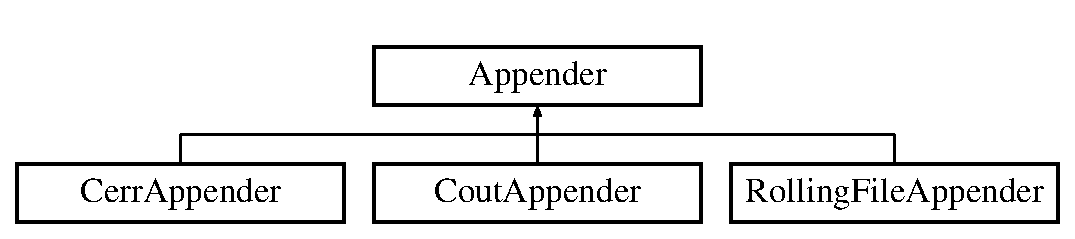
\includegraphics[height=2.000000cm]{class_appender}
\end{center}
\end{figure}
\subsection*{Public Member Functions}
\begin{DoxyCompactItemize}
\item 
\hypertarget{class_appender_a2ad482c763a284fdb8d3dd46c83481ab}{{\bfseries Appender} (const std\-::string name)}\label{class_appender_a2ad482c763a284fdb8d3dd46c83481ab}

\item 
\hypertarget{class_appender_a0e67ca1a0f85984feb8b3088f764b6e7}{virtual void {\bfseries write} (const std\-::string \&line)=0}\label{class_appender_a0e67ca1a0f85984feb8b3088f764b6e7}

\item 
\hypertarget{class_appender_ab042540fad5293516d82b9430e110aed}{virtual void {\bfseries close} ()}\label{class_appender_ab042540fad5293516d82b9430e110aed}

\item 
\hypertarget{class_appender_ae043a5d21e342d46243c12e79cd4e256}{const std\-::string \& {\bfseries name} () const }\label{class_appender_ae043a5d21e342d46243c12e79cd4e256}

\end{DoxyCompactItemize}
\subsection*{Protected Attributes}
\begin{DoxyCompactItemize}
\item 
\hypertarget{class_appender_a6e4dd248b35257d47a5e7befad4ef6aa}{const std\-::string {\bfseries \-\_\-name}}\label{class_appender_a6e4dd248b35257d47a5e7befad4ef6aa}

\end{DoxyCompactItemize}


The documentation for this class was generated from the following files\-:\begin{DoxyCompactItemize}
\item 
repast\-\_\-hpc/logger.\-h\item 
repast\-\_\-hpc/logger.\-cpp\end{DoxyCompactItemize}

\hypertarget{class_appender_builder}{\section{Appender\-Builder Class Reference}
\label{class_appender_builder}\index{Appender\-Builder@{Appender\-Builder}}
}
\subsection*{Public Member Functions}
\begin{DoxyCompactItemize}
\item 
\hypertarget{class_appender_builder_a54ef7bfe2a4bc324957ef673be25ee82}{{\bfseries Appender\-Builder} (const std\-::string name)}\label{class_appender_builder_a54ef7bfe2a4bc324957ef673be25ee82}

\item 
\hypertarget{class_appender_builder_a8f0364cb9215568f44ce573cd8b9b3f0}{\hyperlink{class_appender}{Appender} $\ast$ {\bfseries build} ()}\label{class_appender_builder_a8f0364cb9215568f44ce573cd8b9b3f0}

\end{DoxyCompactItemize}
\subsection*{Public Attributes}
\begin{DoxyCompactItemize}
\item 
\hypertarget{class_appender_builder_ad6d1b5b3182271c7f4dd218b53f7a085}{std\-::string {\bfseries name}}\label{class_appender_builder_ad6d1b5b3182271c7f4dd218b53f7a085}

\item 
\hypertarget{class_appender_builder_a93c3125ddcbec42cd549b39cb856761e}{std\-::string {\bfseries file\-\_\-name}}\label{class_appender_builder_a93c3125ddcbec42cd549b39cb856761e}

\item 
\hypertarget{class_appender_builder_a04ea0440c189ddf1b1e150be593878b8}{long {\bfseries max\-\_\-size}}\label{class_appender_builder_a04ea0440c189ddf1b1e150be593878b8}

\item 
\hypertarget{class_appender_builder_a30816a915e8878a0af244ee45705a4cc}{int {\bfseries max\-\_\-idx}}\label{class_appender_builder_a30816a915e8878a0af244ee45705a4cc}

\end{DoxyCompactItemize}


The documentation for this class was generated from the following files\-:\begin{DoxyCompactItemize}
\item 
repast\-\_\-hpc/logger.\-h\item 
repast\-\_\-hpc/logger.\-cpp\end{DoxyCompactItemize}

\hypertarget{classrepast_1_1_base_grid}{\section{repast\-:\-:Base\-Grid$<$ T, Cell\-Accessor, G\-P\-Transformer, Adder, G\-P\-Type $>$ Class Template Reference}
\label{classrepast_1_1_base_grid}\index{repast\-::\-Base\-Grid$<$ T, Cell\-Accessor, G\-P\-Transformer, Adder, G\-P\-Type $>$@{repast\-::\-Base\-Grid$<$ T, Cell\-Accessor, G\-P\-Transformer, Adder, G\-P\-Type $>$}}
}


Base grid implementation, implementing elements common to both Grids and Continuous\-Spaces.  




{\ttfamily \#include $<$Base\-Grid.\-h$>$}

Inheritance diagram for repast\-:\-:Base\-Grid$<$ T, Cell\-Accessor, G\-P\-Transformer, Adder, G\-P\-Type $>$\-:\begin{figure}[H]
\begin{center}
\leavevmode
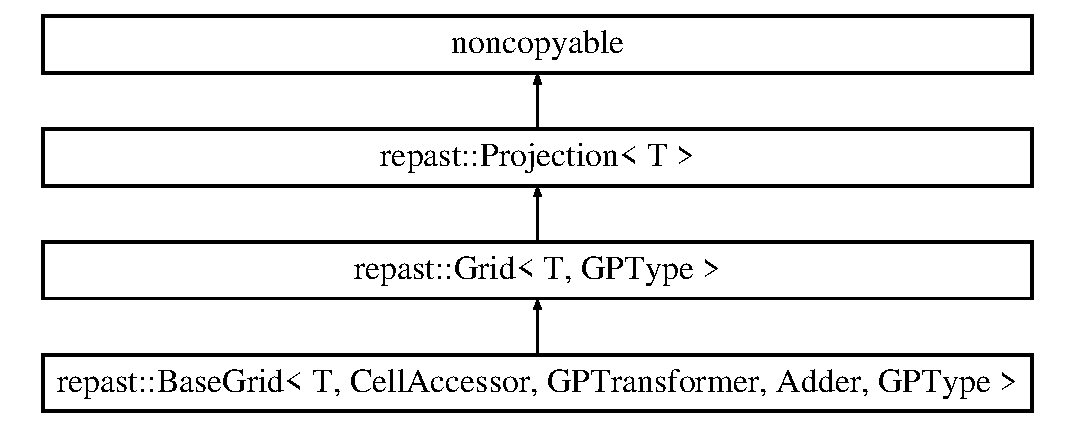
\includegraphics[height=4.000000cm]{classrepast_1_1_base_grid}
\end{center}
\end{figure}
\subsection*{Public Types}
\begin{DoxyCompactItemize}
\item 
\hypertarget{classrepast_1_1_base_grid_ae4de9c96ae3ee3d7021a1e5b3c61b9a6}{typedef \\*
boost\-::transform\-\_\-iterator\\*
$<$ \hyperlink{structrepast_1_1_agent_from_grid_point}{Agent\-From\-Grid\-Point}$<$ T, \\*
G\-P\-Type $>$, Location\-Map\-Const\-Iter $>$ \hyperlink{classrepast_1_1_base_grid_ae4de9c96ae3ee3d7021a1e5b3c61b9a6}{const\-\_\-iterator}}\label{classrepast_1_1_base_grid_ae4de9c96ae3ee3d7021a1e5b3c61b9a6}

\begin{DoxyCompactList}\small\item\em A const iterator over shared\-\_\-ptr$<$\-T$>$. \end{DoxyCompactList}\end{DoxyCompactItemize}
\subsection*{Public Member Functions}
\begin{DoxyCompactItemize}
\item 
\hyperlink{classrepast_1_1_base_grid_a73eae15ca682e2c03a71392c29453d43}{Base\-Grid} (std\-::string \hyperlink{classrepast_1_1_projection_ab60a0ab4f584685780307d7431b61800}{name}, \hyperlink{classrepast_1_1_grid_dimensions}{Grid\-Dimensions} \hyperlink{classrepast_1_1_base_grid_a5f8a2fc16b8aeba026a58fcb374cf05c}{dimensions})
\begin{DoxyCompactList}\small\item\em Creates a \hyperlink{classrepast_1_1_base_grid}{Base\-Grid} with the specified name and dimensions. \end{DoxyCompactList}\item 
virtual bool \hyperlink{classrepast_1_1_base_grid_a648fcba07fdc15b4072b5807b4f1b6b0}{contains} (const \hyperlink{classrepast_1_1_agent_id}{Agent\-Id} \&id)
\begin{DoxyCompactList}\small\item\em Gets whether or not this grid contains the agent with the specified id. \end{DoxyCompactList}\item 
virtual bool \hyperlink{classrepast_1_1_base_grid_a9ef8aae56bb771fa152b10408d718f6e}{get\-Location} (const T $\ast$agent, std\-::vector$<$ G\-P\-Type $>$ \&pt) const 
\begin{DoxyCompactList}\small\item\em Gets the location of this agent and puts it in the specified vector. \end{DoxyCompactList}\item 
virtual bool \hyperlink{classrepast_1_1_base_grid_aa18b424b73ff46fde970ad1e1bb3cdc4}{get\-Location} (const \hyperlink{classrepast_1_1_agent_id}{Agent\-Id} \&id, std\-::vector$<$ G\-P\-Type $>$ \&out) const 
\begin{DoxyCompactList}\small\item\em Gets the location of this agent and puts it in the specified vectors. \end{DoxyCompactList}\item 
virtual T $\ast$ \hyperlink{classrepast_1_1_base_grid_a3710f4aca96eeb3a95a44fe80e0c998a}{get\-Object\-At} (const \hyperlink{classrepast_1_1_point}{Point}$<$ G\-P\-Type $>$ \&pt) const 
\begin{DoxyCompactList}\small\item\em Gets the first object found at the specified point, or N\-U\-L\-L if there is no such object. \end{DoxyCompactList}\item 
virtual void \hyperlink{classrepast_1_1_base_grid_a21d840f3eb758b8f223ca51bf1996328}{get\-Objects\-At} (const \hyperlink{classrepast_1_1_point}{Point}$<$ G\-P\-Type $>$ \&pt, std\-::vector$<$ T $\ast$ $>$ \&out) const 
\begin{DoxyCompactList}\small\item\em Gets all the objects found at the specified point. \end{DoxyCompactList}\item 
virtual bool \hyperlink{classrepast_1_1_base_grid_a40e9d1d23b2e9f4e3d40d87d92595693}{move\-To} (const T $\ast$agent, const std\-::vector$<$ G\-P\-Type $>$ \&new\-Location)
\begin{DoxyCompactList}\small\item\em Moves the specified agent to the specified location. \end{DoxyCompactList}\item 
virtual bool \hyperlink{classrepast_1_1_base_grid_a60f5499f55a0736c07ed87bb37caeae8}{move\-To} (const T $\ast$agent, const \hyperlink{classrepast_1_1_point}{Point}$<$ G\-P\-Type $>$ \&new\-Location)
\begin{DoxyCompactList}\small\item\em Moves the specified agent to the specified location. \end{DoxyCompactList}\item 
virtual bool \hyperlink{classrepast_1_1_base_grid_a3a39996218f4426aa1b2f081d3b44eb4}{move\-To} (const \hyperlink{classrepast_1_1_agent_id}{Agent\-Id} \&id, const std\-::vector$<$ G\-P\-Type $>$ \&new\-Location)
\begin{DoxyCompactList}\small\item\em Moves the specified agent to the specified location. \end{DoxyCompactList}\item 
virtual bool \hyperlink{classrepast_1_1_base_grid_a9f3dbdfe875327dbcc069971de98bc83}{move\-To} (const \hyperlink{classrepast_1_1_agent_id}{Agent\-Id} \&id, const \hyperlink{classrepast_1_1_point}{Point}$<$ G\-P\-Type $>$ \&pt)
\begin{DoxyCompactList}\small\item\em Moves the specified agent to the specified point. \end{DoxyCompactList}\item 
virtual std\-::pair$<$ bool, \hyperlink{classrepast_1_1_point}{Point}\\*
$<$ G\-P\-Type $>$ $>$ \hyperlink{classrepast_1_1_base_grid_a75758e9f795679c0a9c9b92fbd9413af}{move\-By\-Displacement} (const T $\ast$agent, const std\-::vector$<$ G\-P\-Type $>$ \&displacement)
\begin{DoxyCompactList}\small\item\em Moves the specified object from its current location by the specified amount. \end{DoxyCompactList}\item 
\hypertarget{classrepast_1_1_base_grid_a14de646e4c01d6bcd0356669a23af43d}{virtual std\-::pair$<$ bool, \hyperlink{classrepast_1_1_point}{Point}\\*
$<$ G\-P\-Type $>$ $>$ \hyperlink{classrepast_1_1_base_grid_a14de646e4c01d6bcd0356669a23af43d}{move\-By\-Vector} (const T $\ast$agent, double distance, const std\-::vector$<$ double $>$ \&angles\-In\-Radians)}\label{classrepast_1_1_base_grid_a14de646e4c01d6bcd0356669a23af43d}

\begin{DoxyCompactList}\small\item\em doc inherited from \hyperlink{classrepast_1_1_grid}{Grid} \end{DoxyCompactList}\item 
virtual \hyperlink{classrepast_1_1_base_grid_ae4de9c96ae3ee3d7021a1e5b3c61b9a6}{const\-\_\-iterator} \hyperlink{classrepast_1_1_base_grid_ab5aa5a65509879b528bac5b3a9f544b9}{begin} () const 
\begin{DoxyCompactList}\small\item\em Gets an iterator over the agents in this \hyperlink{classrepast_1_1_base_grid}{Base\-Grid} starting with the first agent. \end{DoxyCompactList}\item 
virtual \hyperlink{classrepast_1_1_base_grid_ae4de9c96ae3ee3d7021a1e5b3c61b9a6}{const\-\_\-iterator} \hyperlink{classrepast_1_1_base_grid_ac7eced6c979ccf417b4bbc1c064c687d}{end} () const 
\begin{DoxyCompactList}\small\item\em Gets the end of an iterator over the agents in this \hyperlink{classrepast_1_1_base_grid}{Base\-Grid}. \end{DoxyCompactList}\item 
virtual size\-\_\-t \hyperlink{classrepast_1_1_base_grid_ab1e81ffc9b8f581279a89abf1a4e62e1}{size} () const 
\begin{DoxyCompactList}\small\item\em Gets the number of agents in this \hyperlink{classrepast_1_1_base_grid}{Base\-Grid}. \end{DoxyCompactList}\item 
virtual double \hyperlink{classrepast_1_1_base_grid_a124b5f53a5e96e9ed8e59534e9417f42}{get\-Distance} (const \hyperlink{classrepast_1_1_point}{Point}$<$ G\-P\-Type $>$ \&pt1, const \hyperlink{classrepast_1_1_point}{Point}$<$ G\-P\-Type $>$ \&pt2) const 
\begin{DoxyCompactList}\small\item\em Gets the distance between the two grid points. \end{DoxyCompactList}\item 
virtual double \hyperlink{classrepast_1_1_base_grid_a8075dd20e6d559d453a530943ab9d387}{get\-Distance\-Sq} (const \hyperlink{classrepast_1_1_point}{Point}$<$ G\-P\-Type $>$ \&pt1, const \hyperlink{classrepast_1_1_point}{Point}$<$ G\-P\-Type $>$ \&pt2) const 
\begin{DoxyCompactList}\small\item\em Gets the square of the distance between the two grid points. \end{DoxyCompactList}\item 
virtual void \hyperlink{classrepast_1_1_base_grid_a8c3b8755d2fc2bf75163a0fc76ce1d4a}{get\-Displacement} (const \hyperlink{classrepast_1_1_point}{Point}$<$ G\-P\-Type $>$ \&pt1, const \hyperlink{classrepast_1_1_point}{Point}$<$ G\-P\-Type $>$ \&pt2, std\-::vector$<$ G\-P\-Type $>$ \&out) const 
\begin{DoxyCompactList}\small\item\em Gets vector difference between point 1 and point 2, putting the result in out. \end{DoxyCompactList}\item 
virtual const \hyperlink{classrepast_1_1_grid_dimensions}{Grid\-Dimensions} \hyperlink{classrepast_1_1_base_grid_a5f8a2fc16b8aeba026a58fcb374cf05c}{dimensions} () const 
\begin{DoxyCompactList}\small\item\em Gets the dimensions of this \hyperlink{classrepast_1_1_grid}{Grid}. \end{DoxyCompactList}\item 
virtual void \hyperlink{classrepast_1_1_base_grid_aa5607ff3f29ed7478f0de1d6884e0d7e}{translate} (const \hyperlink{classrepast_1_1_point}{Point}$<$ G\-P\-Type $>$ \&location, const \hyperlink{classrepast_1_1_point}{Point}$<$ G\-P\-Type $>$ \&displacement, std\-::vector$<$ G\-P\-Type $>$ \&out) const 
\begin{DoxyCompactList}\small\item\em Translates the specified location by the specified displacement put the result in out. \end{DoxyCompactList}\item 
virtual void \hyperlink{classrepast_1_1_base_grid_abe3c51f54b40e50e5e2b92b0b1b8e0de}{transform} (const std\-::vector$<$ G\-P\-Type $>$ \&location, std\-::vector$<$ G\-P\-Type $>$ \&out) const 
\begin{DoxyCompactList}\small\item\em Transforms the specified location using the properties (e.\-g. \end{DoxyCompactList}\item 
virtual bool \hyperlink{classrepast_1_1_base_grid_a4dd5ec33acc952ab136f5e2b9886771e}{is\-Periodic} () const 
\begin{DoxyCompactList}\small\item\em Gets whether or not this grid is periodic (i.\-e. \end{DoxyCompactList}\item 
\hypertarget{classrepast_1_1_base_grid_a51685b60fcfb3081007b22559225af8f}{virtual \hyperlink{classrepast_1_1_projection_info_packet}{Projection\-Info\-Packet} $\ast$ {\bfseries get\-Projection\-Info} (\hyperlink{classrepast_1_1_agent_id}{Agent\-Id} id, bool secondary\-Info=false, std\-::set$<$ \hyperlink{classrepast_1_1_agent_id}{Agent\-Id} $>$ $\ast$secondary\-Ids=0, int dest\-Proc=-\/1)}\label{classrepast_1_1_base_grid_a51685b60fcfb3081007b22559225af8f}

\item 
\hypertarget{classrepast_1_1_base_grid_ac95c2c141f8b8365472c2f47df614554}{virtual void {\bfseries update\-Projection\-Info} (\hyperlink{classrepast_1_1_projection_info_packet}{Projection\-Info\-Packet} $\ast$pip, \hyperlink{classrepast_1_1_context}{Context}$<$ T $>$ $\ast$context)}\label{classrepast_1_1_base_grid_ac95c2c141f8b8365472c2f47df614554}

\item 
virtual void \hyperlink{classrepast_1_1_base_grid_a8f718ade5af8285f71151eea824ce3cd}{get\-Agents\-To\-Push} (std\-::set$<$ \hyperlink{classrepast_1_1_agent_id}{Agent\-Id} $>$ \&agents\-To\-Test, std\-::map$<$ int, std\-::set$<$ \hyperlink{classrepast_1_1_agent_id}{Agent\-Id} $>$ $>$ \&agents\-To\-Push)
\begin{DoxyCompactList}\small\item\em Given a set of agents, gets the agents that this projection implementation must 'push' to other processes. \end{DoxyCompactList}\end{DoxyCompactItemize}
\subsection*{Protected Types}
\begin{DoxyCompactItemize}
\item 
\hypertarget{classrepast_1_1_base_grid_acd798e07433e8da414ea2c9ce689f767}{typedef Agent\-Location\-Map\-::iterator {\bfseries Location\-Map\-Iter}}\label{classrepast_1_1_base_grid_acd798e07433e8da414ea2c9ce689f767}

\item 
\hypertarget{classrepast_1_1_base_grid_a42588a88a435a0d3447c4752dd05b3ff}{typedef \\*
Agent\-Location\-Map\-::const\-\_\-iterator {\bfseries Location\-Map\-Const\-Iter}}\label{classrepast_1_1_base_grid_a42588a88a435a0d3447c4752dd05b3ff}

\end{DoxyCompactItemize}
\subsection*{Protected Member Functions}
\begin{DoxyCompactItemize}
\item 
\hypertarget{classrepast_1_1_base_grid_aa119b75be38ed500437d908707752c53}{virtual bool {\bfseries add\-Agent} (boost\-::shared\-\_\-ptr$<$ T $>$ agent)}\label{classrepast_1_1_base_grid_aa119b75be38ed500437d908707752c53}

\item 
\hypertarget{classrepast_1_1_base_grid_ab3a15e82c71ae8467e34adcef97eda10}{virtual void {\bfseries remove\-Agent} (T $\ast$agent)}\label{classrepast_1_1_base_grid_ab3a15e82c71ae8467e34adcef97eda10}

\item 
\hypertarget{classrepast_1_1_base_grid_af2895a0c0f8df474c70fe1f5dc9d7e79}{Location\-Map\-Const\-Iter {\bfseries locations\-Begin} () const }\label{classrepast_1_1_base_grid_af2895a0c0f8df474c70fe1f5dc9d7e79}

\item 
\hypertarget{classrepast_1_1_base_grid_a4e46f683b8f413cd4ef761791436d0c3}{Location\-Map\-Const\-Iter {\bfseries locations\-End} () const }\label{classrepast_1_1_base_grid_a4e46f683b8f413cd4ef761791436d0c3}

\item 
\hypertarget{classrepast_1_1_base_grid_aab0d37e733a70b57f045f934ca9aa5f6}{T $\ast$ {\bfseries get} (const \hyperlink{classrepast_1_1_agent_id}{Agent\-Id} \&id)}\label{classrepast_1_1_base_grid_aab0d37e733a70b57f045f934ca9aa5f6}

\end{DoxyCompactItemize}
\subsection*{Protected Attributes}
\begin{DoxyCompactItemize}
\item 
\hypertarget{classrepast_1_1_base_grid_a4116ebd80bf98c4d403bfdf1d7891b5e}{G\-P\-Transformer {\bfseries gp\-Transformer}}\label{classrepast_1_1_base_grid_a4116ebd80bf98c4d403bfdf1d7891b5e}

\item 
\hypertarget{classrepast_1_1_base_grid_a268f1e662d2423eb06554c1da59f22c2}{Adder {\bfseries adder}}\label{classrepast_1_1_base_grid_a268f1e662d2423eb06554c1da59f22c2}

\end{DoxyCompactItemize}


\subsection{Detailed Description}
\subsubsection*{template$<$typename T, typename Cell\-Accessor, typename G\-P\-Transformer, typename Adder, typename G\-P\-Type$>$class repast\-::\-Base\-Grid$<$ T, Cell\-Accessor, G\-P\-Transformer, Adder, G\-P\-Type $>$}

Base grid implementation, implementing elements common to both Grids and Continuous\-Spaces. 

Standard grid and space types that provide defaults for the various template parameters can be found in Space in Space.\-h


\begin{DoxyTemplParams}{Template Parameters}
{\em T} & the type of objects contained by this \hyperlink{classrepast_1_1_base_grid}{Base\-Grid} (generally the type of agents) \\
\hline
{\em Cell\-Accessor} & implements the actual storage for the grid. \\
\hline
{\em G\-P\-Transformer} & transforms cell points according to the topology (e.\-g. periodic) of the \hyperlink{classrepast_1_1_base_grid}{Base\-Grid}. \\
\hline
{\em Adder} & determines how objects are added to the grid from its associated context. \\
\hline
{\em G\-P\-Type} & the coordinate type of the grid point locations; this must be an int or a double. \\
\hline
\end{DoxyTemplParams}


\subsection{Constructor \& Destructor Documentation}
\hypertarget{classrepast_1_1_base_grid_a73eae15ca682e2c03a71392c29453d43}{\index{repast\-::\-Base\-Grid@{repast\-::\-Base\-Grid}!Base\-Grid@{Base\-Grid}}
\index{Base\-Grid@{Base\-Grid}!repast::BaseGrid@{repast\-::\-Base\-Grid}}
\subsubsection[{Base\-Grid}]{\setlength{\rightskip}{0pt plus 5cm}template$<$typename T , typename Cell\-Accessor , typename G\-P\-Transformer , typename Adder , typename G\-P\-Type $>$ {\bf repast\-::\-Base\-Grid}$<$ T, Cell\-Accessor, G\-P\-Transformer, Adder, G\-P\-Type $>$\-::{\bf Base\-Grid} (
\begin{DoxyParamCaption}
\item[{std\-::string}]{name, }
\item[{{\bf Grid\-Dimensions}}]{dimensions}
\end{DoxyParamCaption}
)}}\label{classrepast_1_1_base_grid_a73eae15ca682e2c03a71392c29453d43}


Creates a \hyperlink{classrepast_1_1_base_grid}{Base\-Grid} with the specified name and dimensions. 


\begin{DoxyParams}{Parameters}
{\em name} & the name of the \hyperlink{classrepast_1_1_base_grid}{Base\-Grid} \\
\hline
{\em dimensions} & the dimensions of the \hyperlink{classrepast_1_1_base_grid}{Base\-Grid} \\
\hline
\end{DoxyParams}


\subsection{Member Function Documentation}
\hypertarget{classrepast_1_1_base_grid_ab5aa5a65509879b528bac5b3a9f544b9}{\index{repast\-::\-Base\-Grid@{repast\-::\-Base\-Grid}!begin@{begin}}
\index{begin@{begin}!repast::BaseGrid@{repast\-::\-Base\-Grid}}
\subsubsection[{begin}]{\setlength{\rightskip}{0pt plus 5cm}template$<$typename T, typename Cell\-Accessor, typename G\-P\-Transformer, typename Adder, typename G\-P\-Type$>$ virtual {\bf const\-\_\-iterator} {\bf repast\-::\-Base\-Grid}$<$ T, Cell\-Accessor, G\-P\-Transformer, Adder, G\-P\-Type $>$\-::begin (
\begin{DoxyParamCaption}
{}
\end{DoxyParamCaption}
) const\hspace{0.3cm}{\ttfamily [inline]}, {\ttfamily [virtual]}}}\label{classrepast_1_1_base_grid_ab5aa5a65509879b528bac5b3a9f544b9}


Gets an iterator over the agents in this \hyperlink{classrepast_1_1_base_grid}{Base\-Grid} starting with the first agent. 

The iterator derefrences into shared\-\_\-ptr$<$\-T$>$. The actual agent can be accessed by derefrenceing the iter\-: ($\ast$iter)-\/$>$get\-Id() for example.

\begin{DoxyReturn}{Returns}
an iterator over the agents in this \hyperlink{classrepast_1_1_base_grid}{Base\-Grid} starting with the first agent. 
\end{DoxyReturn}
\hypertarget{classrepast_1_1_base_grid_a648fcba07fdc15b4072b5807b4f1b6b0}{\index{repast\-::\-Base\-Grid@{repast\-::\-Base\-Grid}!contains@{contains}}
\index{contains@{contains}!repast::BaseGrid@{repast\-::\-Base\-Grid}}
\subsubsection[{contains}]{\setlength{\rightskip}{0pt plus 5cm}template$<$typename T , typename Cell\-Accessor , typename G\-P\-Transformer , typename Adder , typename G\-P\-Type $>$ bool {\bf repast\-::\-Base\-Grid}$<$ T, Cell\-Accessor, G\-P\-Transformer, Adder, G\-P\-Type $>$\-::contains (
\begin{DoxyParamCaption}
\item[{const {\bf Agent\-Id} \&}]{id}
\end{DoxyParamCaption}
)\hspace{0.3cm}{\ttfamily [virtual]}}}\label{classrepast_1_1_base_grid_a648fcba07fdc15b4072b5807b4f1b6b0}


Gets whether or not this grid contains the agent with the specified id. 


\begin{DoxyParams}{Parameters}
{\em id} & the id of the agent to check\\
\hline
\end{DoxyParams}
\begin{DoxyReturn}{Returns}
true if the grid contains the agent, otherwise false. 
\end{DoxyReturn}


Implements \hyperlink{classrepast_1_1_grid_a022599f875eeb1e72c11766500d8282c}{repast\-::\-Grid$<$ T, G\-P\-Type $>$}.

\hypertarget{classrepast_1_1_base_grid_a5f8a2fc16b8aeba026a58fcb374cf05c}{\index{repast\-::\-Base\-Grid@{repast\-::\-Base\-Grid}!dimensions@{dimensions}}
\index{dimensions@{dimensions}!repast::BaseGrid@{repast\-::\-Base\-Grid}}
\subsubsection[{dimensions}]{\setlength{\rightskip}{0pt plus 5cm}template$<$typename T, typename Cell\-Accessor, typename G\-P\-Transformer, typename Adder, typename G\-P\-Type$>$ virtual const {\bf Grid\-Dimensions} {\bf repast\-::\-Base\-Grid}$<$ T, Cell\-Accessor, G\-P\-Transformer, Adder, G\-P\-Type $>$\-::dimensions (
\begin{DoxyParamCaption}
{}
\end{DoxyParamCaption}
) const\hspace{0.3cm}{\ttfamily [inline]}, {\ttfamily [virtual]}}}\label{classrepast_1_1_base_grid_a5f8a2fc16b8aeba026a58fcb374cf05c}


Gets the dimensions of this \hyperlink{classrepast_1_1_grid}{Grid}. 

\begin{DoxyReturn}{Returns}
the dimensions of this \hyperlink{classrepast_1_1_grid}{Grid}. 
\end{DoxyReturn}


Implements \hyperlink{classrepast_1_1_grid_ac6a979a6491565212ae44b8bfbbc9393}{repast\-::\-Grid$<$ T, G\-P\-Type $>$}.



Reimplemented in \hyperlink{classrepast_1_1_shared_base_grid_a9ec19652232000368ec1fe98ff47e121}{repast\-::\-Shared\-Base\-Grid$<$ T, G\-P\-Transformer, Adder, G\-P\-Type $>$}, \hyperlink{classrepast_1_1_shared_base_grid_a9ec19652232000368ec1fe98ff47e121}{repast\-::\-Shared\-Base\-Grid$<$ T, G\-P\-Transformer, Adder, int $>$}, and \hyperlink{classrepast_1_1_shared_base_grid_a9ec19652232000368ec1fe98ff47e121}{repast\-::\-Shared\-Base\-Grid$<$ T, G\-P\-Transformer, Adder, double $>$}.

\hypertarget{classrepast_1_1_base_grid_ac7eced6c979ccf417b4bbc1c064c687d}{\index{repast\-::\-Base\-Grid@{repast\-::\-Base\-Grid}!end@{end}}
\index{end@{end}!repast::BaseGrid@{repast\-::\-Base\-Grid}}
\subsubsection[{end}]{\setlength{\rightskip}{0pt plus 5cm}template$<$typename T, typename Cell\-Accessor, typename G\-P\-Transformer, typename Adder, typename G\-P\-Type$>$ virtual {\bf const\-\_\-iterator} {\bf repast\-::\-Base\-Grid}$<$ T, Cell\-Accessor, G\-P\-Transformer, Adder, G\-P\-Type $>$\-::end (
\begin{DoxyParamCaption}
{}
\end{DoxyParamCaption}
) const\hspace{0.3cm}{\ttfamily [inline]}, {\ttfamily [virtual]}}}\label{classrepast_1_1_base_grid_ac7eced6c979ccf417b4bbc1c064c687d}


Gets the end of an iterator over the agents in this \hyperlink{classrepast_1_1_base_grid}{Base\-Grid}. 

\begin{DoxyReturn}{Returns}
the end of an iterator over the agents in this \hyperlink{classrepast_1_1_base_grid}{Base\-Grid}. 
\end{DoxyReturn}
\hypertarget{classrepast_1_1_base_grid_a8f718ade5af8285f71151eea824ce3cd}{\index{repast\-::\-Base\-Grid@{repast\-::\-Base\-Grid}!get\-Agents\-To\-Push@{get\-Agents\-To\-Push}}
\index{get\-Agents\-To\-Push@{get\-Agents\-To\-Push}!repast::BaseGrid@{repast\-::\-Base\-Grid}}
\subsubsection[{get\-Agents\-To\-Push}]{\setlength{\rightskip}{0pt plus 5cm}template$<$typename T, typename Cell\-Accessor, typename G\-P\-Transformer, typename Adder, typename G\-P\-Type$>$ virtual void {\bf repast\-::\-Base\-Grid}$<$ T, Cell\-Accessor, G\-P\-Transformer, Adder, G\-P\-Type $>$\-::get\-Agents\-To\-Push (
\begin{DoxyParamCaption}
\item[{std\-::set$<$ {\bf Agent\-Id} $>$ \&}]{agents\-To\-Test, }
\item[{std\-::map$<$ int, std\-::set$<$ {\bf Agent\-Id} $>$ $>$ \&}]{agents\-To\-Push}
\end{DoxyParamCaption}
)\hspace{0.3cm}{\ttfamily [inline]}, {\ttfamily [virtual]}}}\label{classrepast_1_1_base_grid_a8f718ade5af8285f71151eea824ce3cd}


Given a set of agents, gets the agents that this projection implementation must 'push' to other processes. 

Generally spaces must push agents that are in 'buffer zones' and graphs must push local agents that are vertices to master edges where the other vertex is non-\/ local. The results are returned per-\/process in the agents\-To\-Push map. 

Implements \hyperlink{classrepast_1_1_grid_aa83b294fc8765e2f8ee44d8238855460}{repast\-::\-Grid$<$ T, G\-P\-Type $>$}.



Reimplemented in \hyperlink{classrepast_1_1_shared_base_grid_ab1486e7698288efc1218653d4e5e1e15}{repast\-::\-Shared\-Base\-Grid$<$ T, G\-P\-Transformer, Adder, G\-P\-Type $>$}, \hyperlink{classrepast_1_1_shared_base_grid_ab1486e7698288efc1218653d4e5e1e15}{repast\-::\-Shared\-Base\-Grid$<$ T, G\-P\-Transformer, Adder, int $>$}, \hyperlink{classrepast_1_1_shared_base_grid_ab1486e7698288efc1218653d4e5e1e15}{repast\-::\-Shared\-Base\-Grid$<$ T, G\-P\-Transformer, Adder, double $>$}, and \hyperlink{classrepast_1_1_shared_discrete_space_a1f690e82e6b7ea6a279db020e12b4d21}{repast\-::\-Shared\-Discrete\-Space$<$ T, G\-P\-Transformer, Adder $>$}.

\hypertarget{classrepast_1_1_base_grid_a8c3b8755d2fc2bf75163a0fc76ce1d4a}{\index{repast\-::\-Base\-Grid@{repast\-::\-Base\-Grid}!get\-Displacement@{get\-Displacement}}
\index{get\-Displacement@{get\-Displacement}!repast::BaseGrid@{repast\-::\-Base\-Grid}}
\subsubsection[{get\-Displacement}]{\setlength{\rightskip}{0pt plus 5cm}template$<$typename T , typename Cell\-Accessor , typename G\-P\-Transformer , typename Adder , typename G\-P\-Type$>$ void {\bf repast\-::\-Base\-Grid}$<$ T, Cell\-Accessor, G\-P\-Transformer, Adder, G\-P\-Type $>$\-::get\-Displacement (
\begin{DoxyParamCaption}
\item[{const {\bf Point}$<$ G\-P\-Type $>$ \&}]{pt1, }
\item[{const {\bf Point}$<$ G\-P\-Type $>$ \&}]{pt2, }
\item[{std\-::vector$<$ G\-P\-Type $>$ \&}]{out}
\end{DoxyParamCaption}
) const\hspace{0.3cm}{\ttfamily [virtual]}}}\label{classrepast_1_1_base_grid_a8c3b8755d2fc2bf75163a0fc76ce1d4a}


Gets vector difference between point 1 and point 2, putting the result in out. 


\begin{DoxyParams}[1]{Parameters}
 & {\em p1} & the first point \\
\hline
 & {\em p2} & the second point \\
\hline
\mbox{\tt out}  & {\em the} & vector where the difference will be put \\
\hline
\end{DoxyParams}


Implements \hyperlink{classrepast_1_1_grid_a23236c2387ba343121dbf71901dbb341}{repast\-::\-Grid$<$ T, G\-P\-Type $>$}.

\hypertarget{classrepast_1_1_base_grid_a124b5f53a5e96e9ed8e59534e9417f42}{\index{repast\-::\-Base\-Grid@{repast\-::\-Base\-Grid}!get\-Distance@{get\-Distance}}
\index{get\-Distance@{get\-Distance}!repast::BaseGrid@{repast\-::\-Base\-Grid}}
\subsubsection[{get\-Distance}]{\setlength{\rightskip}{0pt plus 5cm}template$<$typename T , typename Cell\-Accessor , typename G\-P\-Transformer , typename Adder , typename G\-P\-Type$>$ double {\bf repast\-::\-Base\-Grid}$<$ T, Cell\-Accessor, G\-P\-Transformer, Adder, G\-P\-Type $>$\-::get\-Distance (
\begin{DoxyParamCaption}
\item[{const {\bf Point}$<$ G\-P\-Type $>$ \&}]{pt1, }
\item[{const {\bf Point}$<$ G\-P\-Type $>$ \&}]{pt2}
\end{DoxyParamCaption}
) const\hspace{0.3cm}{\ttfamily [virtual]}}}\label{classrepast_1_1_base_grid_a124b5f53a5e96e9ed8e59534e9417f42}


Gets the distance between the two grid points. 


\begin{DoxyParams}{Parameters}
{\em p1} & the first point \\
\hline
{\em p2} & the second point\\
\hline
\end{DoxyParams}
\begin{DoxyReturn}{Returns}
the distance between pt1 and pt2. 
\end{DoxyReturn}


Implements \hyperlink{classrepast_1_1_grid_a27213b5f9decf10e1c99a5a7b4ae387a}{repast\-::\-Grid$<$ T, G\-P\-Type $>$}.

\hypertarget{classrepast_1_1_base_grid_a8075dd20e6d559d453a530943ab9d387}{\index{repast\-::\-Base\-Grid@{repast\-::\-Base\-Grid}!get\-Distance\-Sq@{get\-Distance\-Sq}}
\index{get\-Distance\-Sq@{get\-Distance\-Sq}!repast::BaseGrid@{repast\-::\-Base\-Grid}}
\subsubsection[{get\-Distance\-Sq}]{\setlength{\rightskip}{0pt plus 5cm}template$<$typename T , typename Cell\-Accessor , typename G\-P\-Transformer , typename Adder , typename G\-P\-Type$>$ double {\bf repast\-::\-Base\-Grid}$<$ T, Cell\-Accessor, G\-P\-Transformer, Adder, G\-P\-Type $>$\-::get\-Distance\-Sq (
\begin{DoxyParamCaption}
\item[{const {\bf Point}$<$ G\-P\-Type $>$ \&}]{pt1, }
\item[{const {\bf Point}$<$ G\-P\-Type $>$ \&}]{pt2}
\end{DoxyParamCaption}
) const\hspace{0.3cm}{\ttfamily [virtual]}}}\label{classrepast_1_1_base_grid_a8075dd20e6d559d453a530943ab9d387}


Gets the square of the distance between the two grid points. 


\begin{DoxyParams}{Parameters}
{\em p1} & the first point \\
\hline
{\em p2} & the second point\\
\hline
\end{DoxyParams}
\begin{DoxyReturn}{Returns}
the square of the distance between pt1 and pt2. 
\end{DoxyReturn}


Implements \hyperlink{classrepast_1_1_grid_a456d00d28995a48b41b8f6c84817879e}{repast\-::\-Grid$<$ T, G\-P\-Type $>$}.

\hypertarget{classrepast_1_1_base_grid_a9ef8aae56bb771fa152b10408d718f6e}{\index{repast\-::\-Base\-Grid@{repast\-::\-Base\-Grid}!get\-Location@{get\-Location}}
\index{get\-Location@{get\-Location}!repast::BaseGrid@{repast\-::\-Base\-Grid}}
\subsubsection[{get\-Location}]{\setlength{\rightskip}{0pt plus 5cm}template$<$typename T, typename Cell\-Accessor , typename G\-P\-Transformer , typename Adder , typename G\-P\-Type$>$ bool {\bf repast\-::\-Base\-Grid}$<$ T, Cell\-Accessor, G\-P\-Transformer, Adder, G\-P\-Type $>$\-::get\-Location (
\begin{DoxyParamCaption}
\item[{const T $\ast$}]{agent, }
\item[{std\-::vector$<$ G\-P\-Type $>$ \&}]{out}
\end{DoxyParamCaption}
) const\hspace{0.3cm}{\ttfamily [virtual]}}}\label{classrepast_1_1_base_grid_a9ef8aae56bb771fa152b10408d718f6e}


Gets the location of this agent and puts it in the specified vector. 

The x coordinate will be the first value, the y the second and so on.


\begin{DoxyParams}[1]{Parameters}
 & {\em agent} & the agent whose location we want to get \\
\hline
\mbox{\tt out}  & {\em the} & vector where the agents location will be put\\
\hline
\end{DoxyParams}
\begin{DoxyReturn}{Returns}
true if the location was successfully found, otherwise false. 
\end{DoxyReturn}


Implements \hyperlink{classrepast_1_1_grid_a159a33da91ef58dbd8ca88829d82ca36}{repast\-::\-Grid$<$ T, G\-P\-Type $>$}.

\hypertarget{classrepast_1_1_base_grid_aa18b424b73ff46fde970ad1e1bb3cdc4}{\index{repast\-::\-Base\-Grid@{repast\-::\-Base\-Grid}!get\-Location@{get\-Location}}
\index{get\-Location@{get\-Location}!repast::BaseGrid@{repast\-::\-Base\-Grid}}
\subsubsection[{get\-Location}]{\setlength{\rightskip}{0pt plus 5cm}template$<$typename T, typename Cell\-Accessor , typename G\-P\-Transformer , typename Adder , typename G\-P\-Type$>$ bool {\bf repast\-::\-Base\-Grid}$<$ T, Cell\-Accessor, G\-P\-Transformer, Adder, G\-P\-Type $>$\-::get\-Location (
\begin{DoxyParamCaption}
\item[{const {\bf Agent\-Id} \&}]{id, }
\item[{std\-::vector$<$ G\-P\-Type $>$ \&}]{out}
\end{DoxyParamCaption}
) const\hspace{0.3cm}{\ttfamily [virtual]}}}\label{classrepast_1_1_base_grid_aa18b424b73ff46fde970ad1e1bb3cdc4}


Gets the location of this agent and puts it in the specified vectors. 

The x coordinate will be the first value, the y the second and so on.


\begin{DoxyParams}[1]{Parameters}
 & {\em id} & the id of the agent whose location we want to get \\
\hline
\mbox{\tt out}  & {\em out} & the agent's location will be put into this vector\\
\hline
\end{DoxyParams}
\begin{DoxyReturn}{Returns}
true if the location was successfully found, otherwise false. 
\end{DoxyReturn}


Implements \hyperlink{classrepast_1_1_grid_a6fef590f66b69e4a06207df59d1b2737}{repast\-::\-Grid$<$ T, G\-P\-Type $>$}.

\hypertarget{classrepast_1_1_base_grid_a3710f4aca96eeb3a95a44fe80e0c998a}{\index{repast\-::\-Base\-Grid@{repast\-::\-Base\-Grid}!get\-Object\-At@{get\-Object\-At}}
\index{get\-Object\-At@{get\-Object\-At}!repast::BaseGrid@{repast\-::\-Base\-Grid}}
\subsubsection[{get\-Object\-At}]{\setlength{\rightskip}{0pt plus 5cm}template$<$typename T , typename Cell\-Accessor , typename G\-P\-Transformer , typename Adder , typename G\-P\-Type$>$ T $\ast$ {\bf repast\-::\-Base\-Grid}$<$ T, Cell\-Accessor, G\-P\-Transformer, Adder, G\-P\-Type $>$\-::get\-Object\-At (
\begin{DoxyParamCaption}
\item[{const {\bf Point}$<$ G\-P\-Type $>$ \&}]{pt}
\end{DoxyParamCaption}
) const\hspace{0.3cm}{\ttfamily [virtual]}}}\label{classrepast_1_1_base_grid_a3710f4aca96eeb3a95a44fe80e0c998a}


Gets the first object found at the specified point, or N\-U\-L\-L if there is no such object. 

\begin{DoxyReturn}{Returns}
the first object found at the specified point, or N\-U\-L\-L if there is no such object. 
\end{DoxyReturn}


Implements \hyperlink{classrepast_1_1_grid_a8b77b072353aed6f06b6d02e21ee9879}{repast\-::\-Grid$<$ T, G\-P\-Type $>$}.

\hypertarget{classrepast_1_1_base_grid_a21d840f3eb758b8f223ca51bf1996328}{\index{repast\-::\-Base\-Grid@{repast\-::\-Base\-Grid}!get\-Objects\-At@{get\-Objects\-At}}
\index{get\-Objects\-At@{get\-Objects\-At}!repast::BaseGrid@{repast\-::\-Base\-Grid}}
\subsubsection[{get\-Objects\-At}]{\setlength{\rightskip}{0pt plus 5cm}template$<$typename T, typename Cell\-Accessor , typename G\-P\-Transformer , typename Adder , typename G\-P\-Type$>$ void {\bf repast\-::\-Base\-Grid}$<$ T, Cell\-Accessor, G\-P\-Transformer, Adder, G\-P\-Type $>$\-::get\-Objects\-At (
\begin{DoxyParamCaption}
\item[{const {\bf Point}$<$ G\-P\-Type $>$ \&}]{pt, }
\item[{std\-::vector$<$ T $\ast$ $>$ \&}]{out}
\end{DoxyParamCaption}
) const\hspace{0.3cm}{\ttfamily [virtual]}}}\label{classrepast_1_1_base_grid_a21d840f3eb758b8f223ca51bf1996328}


Gets all the objects found at the specified point. 

The found objects will be put into the out parameter.


\begin{DoxyParams}[1]{Parameters}
 & {\em pt} & the point to get all the objects at \\
\hline
\mbox{\tt out}  & {\em out} & the vector into which the found objects will be put \\
\hline
\end{DoxyParams}


Implements \hyperlink{classrepast_1_1_grid_aaa3a1fd92707079f7dd4805e36ca83ff}{repast\-::\-Grid$<$ T, G\-P\-Type $>$}.

\hypertarget{classrepast_1_1_base_grid_a4dd5ec33acc952ab136f5e2b9886771e}{\index{repast\-::\-Base\-Grid@{repast\-::\-Base\-Grid}!is\-Periodic@{is\-Periodic}}
\index{is\-Periodic@{is\-Periodic}!repast::BaseGrid@{repast\-::\-Base\-Grid}}
\subsubsection[{is\-Periodic}]{\setlength{\rightskip}{0pt plus 5cm}template$<$typename T, typename Cell\-Accessor, typename G\-P\-Transformer, typename Adder, typename G\-P\-Type$>$ virtual bool {\bf repast\-::\-Base\-Grid}$<$ T, Cell\-Accessor, G\-P\-Transformer, Adder, G\-P\-Type $>$\-::is\-Periodic (
\begin{DoxyParamCaption}
{}
\end{DoxyParamCaption}
) const\hspace{0.3cm}{\ttfamily [inline]}, {\ttfamily [virtual]}}}\label{classrepast_1_1_base_grid_a4dd5ec33acc952ab136f5e2b9886771e}


Gets whether or not this grid is periodic (i.\-e. 

toroidal).

\begin{DoxyReturn}{Returns}
true if this \hyperlink{classrepast_1_1_grid}{Grid} is periodic, otherwise false. 
\end{DoxyReturn}


Implements \hyperlink{classrepast_1_1_grid_a81e7eb612dabbf2fb4b3f1190cd92f88}{repast\-::\-Grid$<$ T, G\-P\-Type $>$}.

\hypertarget{classrepast_1_1_base_grid_a75758e9f795679c0a9c9b92fbd9413af}{\index{repast\-::\-Base\-Grid@{repast\-::\-Base\-Grid}!move\-By\-Displacement@{move\-By\-Displacement}}
\index{move\-By\-Displacement@{move\-By\-Displacement}!repast::BaseGrid@{repast\-::\-Base\-Grid}}
\subsubsection[{move\-By\-Displacement}]{\setlength{\rightskip}{0pt plus 5cm}template$<$typename T, typename Cell\-Accessor , typename G\-P\-Transformer , typename Adder , typename G\-P\-Type$>$ std\-::pair$<$ bool, {\bf Point}$<$ G\-P\-Type $>$ $>$ {\bf repast\-::\-Base\-Grid}$<$ T, Cell\-Accessor, G\-P\-Transformer, Adder, G\-P\-Type $>$\-::move\-By\-Displacement (
\begin{DoxyParamCaption}
\item[{const T $\ast$}]{agent, }
\item[{const std\-::vector$<$ G\-P\-Type $>$ \&}]{displacement}
\end{DoxyParamCaption}
)\hspace{0.3cm}{\ttfamily [virtual]}}}\label{classrepast_1_1_base_grid_a75758e9f795679c0a9c9b92fbd9413af}


Moves the specified object from its current location by the specified amount. 

For example {\ttfamily move\-By\-Displacement(object, 3, -\/2, 1)} will move the object by 3 along the x-\/axis, -\/2 along the y and 1 along the z. The displacement argument can be less than the number of dimensions in the space in which case the remaining argument will be set to 0. For example, {\ttfamily move\-By\-Displacement(object, 3)} will move the object 3 along the x-\/axis and 0 along the y and z axes, assuming a 3\-D grid.


\begin{DoxyParams}{Parameters}
{\em agent} & the object to move \\
\hline
{\em displacement} & the amount to move the object \\
\hline
\end{DoxyParams}
\begin{DoxyReturn}{Returns}
a pair containing a bool that indicates whether the move was a success or not, and the point where the agent was moved to. 
\end{DoxyReturn}


Implements \hyperlink{classrepast_1_1_grid_a20efd6bdadf8dac405542de7e33f6b9e}{repast\-::\-Grid$<$ T, G\-P\-Type $>$}.

\hypertarget{classrepast_1_1_base_grid_a40e9d1d23b2e9f4e3d40d87d92595693}{\index{repast\-::\-Base\-Grid@{repast\-::\-Base\-Grid}!move\-To@{move\-To}}
\index{move\-To@{move\-To}!repast::BaseGrid@{repast\-::\-Base\-Grid}}
\subsubsection[{move\-To}]{\setlength{\rightskip}{0pt plus 5cm}template$<$typename T, typename Cell\-Accessor , typename G\-P\-Transformer , typename Adder , typename G\-P\-Type$>$ bool {\bf repast\-::\-Base\-Grid}$<$ T, Cell\-Accessor, G\-P\-Transformer, Adder, G\-P\-Type $>$\-::move\-To (
\begin{DoxyParamCaption}
\item[{const T $\ast$}]{agent, }
\item[{const std\-::vector$<$ G\-P\-Type $>$ \&}]{new\-Location}
\end{DoxyParamCaption}
)\hspace{0.3cm}{\ttfamily [virtual]}}}\label{classrepast_1_1_base_grid_a40e9d1d23b2e9f4e3d40d87d92595693}


Moves the specified agent to the specified location. 

Returns true if the move was successful otherwise false. The agent must be already added to the context associated with this space, otherwise this throws an out\-\_\-of\-\_\-range exception if the new location out of bounds.


\begin{DoxyParams}{Parameters}
{\em agent} & the agent to move \\
\hline
{\em new\-Location} & the location to move to\\
\hline
\end{DoxyParams}
\begin{DoxyReturn}{Returns}
true if the move was successful, otherwise false 
\end{DoxyReturn}
\hypertarget{classrepast_1_1_base_grid_a60f5499f55a0736c07ed87bb37caeae8}{\index{repast\-::\-Base\-Grid@{repast\-::\-Base\-Grid}!move\-To@{move\-To}}
\index{move\-To@{move\-To}!repast::BaseGrid@{repast\-::\-Base\-Grid}}
\subsubsection[{move\-To}]{\setlength{\rightskip}{0pt plus 5cm}template$<$typename T, typename Cell\-Accessor , typename G\-P\-Transformer , typename Adder , typename G\-P\-Type$>$ bool {\bf repast\-::\-Base\-Grid}$<$ T, Cell\-Accessor, G\-P\-Transformer, Adder, G\-P\-Type $>$\-::move\-To (
\begin{DoxyParamCaption}
\item[{const T $\ast$}]{agent, }
\item[{const {\bf Point}$<$ G\-P\-Type $>$ \&}]{new\-Location}
\end{DoxyParamCaption}
)\hspace{0.3cm}{\ttfamily [virtual]}}}\label{classrepast_1_1_base_grid_a60f5499f55a0736c07ed87bb37caeae8}


Moves the specified agent to the specified location. 

Returns true if the move was successful otherwise false. The agent must be already added to the context associated with this space, otherwise this throws an out\-\_\-of\-\_\-range exception if the new location out of bounds.


\begin{DoxyParams}{Parameters}
{\em agent} & the agent to move \\
\hline
{\em new\-Location} & the location to move to\\
\hline
\end{DoxyParams}
\begin{DoxyReturn}{Returns}
true if the move was successful, otherwise false 
\end{DoxyReturn}
\hypertarget{classrepast_1_1_base_grid_a3a39996218f4426aa1b2f081d3b44eb4}{\index{repast\-::\-Base\-Grid@{repast\-::\-Base\-Grid}!move\-To@{move\-To}}
\index{move\-To@{move\-To}!repast::BaseGrid@{repast\-::\-Base\-Grid}}
\subsubsection[{move\-To}]{\setlength{\rightskip}{0pt plus 5cm}template$<$typename T, typename Cell\-Accessor , typename G\-P\-Transformer , typename Adder , typename G\-P\-Type$>$ bool {\bf repast\-::\-Base\-Grid}$<$ T, Cell\-Accessor, G\-P\-Transformer, Adder, G\-P\-Type $>$\-::move\-To (
\begin{DoxyParamCaption}
\item[{const {\bf Agent\-Id} \&}]{id, }
\item[{const std\-::vector$<$ G\-P\-Type $>$ \&}]{new\-Location}
\end{DoxyParamCaption}
)\hspace{0.3cm}{\ttfamily [virtual]}}}\label{classrepast_1_1_base_grid_a3a39996218f4426aa1b2f081d3b44eb4}


Moves the specified agent to the specified location. 

Returns true if the move was successful otherwise false. The agent must be already added to the context associated with this space, otherwise this throws an out\-\_\-of\-\_\-range exception if the new location out of bounds.


\begin{DoxyParams}{Parameters}
{\em id} & the id of the agent to move \\
\hline
{\em new\-Location} & the location to move to\\
\hline
\end{DoxyParams}
\begin{DoxyReturn}{Returns}
true if the move was successful, otherwise false 
\end{DoxyReturn}


Reimplemented in \hyperlink{classrepast_1_1_shared_base_grid_a480fc6f517d1bb098c7ee47450fba522}{repast\-::\-Shared\-Base\-Grid$<$ T, G\-P\-Transformer, Adder, G\-P\-Type $>$}, \hyperlink{classrepast_1_1_shared_base_grid_a480fc6f517d1bb098c7ee47450fba522}{repast\-::\-Shared\-Base\-Grid$<$ T, G\-P\-Transformer, Adder, int $>$}, and \hyperlink{classrepast_1_1_shared_base_grid_a480fc6f517d1bb098c7ee47450fba522}{repast\-::\-Shared\-Base\-Grid$<$ T, G\-P\-Transformer, Adder, double $>$}.

\hypertarget{classrepast_1_1_base_grid_a9f3dbdfe875327dbcc069971de98bc83}{\index{repast\-::\-Base\-Grid@{repast\-::\-Base\-Grid}!move\-To@{move\-To}}
\index{move\-To@{move\-To}!repast::BaseGrid@{repast\-::\-Base\-Grid}}
\subsubsection[{move\-To}]{\setlength{\rightskip}{0pt plus 5cm}template$<$typename T, typename Cell\-Accessor , typename G\-P\-Transformer , typename Adder , typename G\-P\-Type$>$ bool {\bf repast\-::\-Base\-Grid}$<$ T, Cell\-Accessor, G\-P\-Transformer, Adder, G\-P\-Type $>$\-::move\-To (
\begin{DoxyParamCaption}
\item[{const {\bf Agent\-Id} \&}]{id, }
\item[{const {\bf Point}$<$ G\-P\-Type $>$ \&}]{pt}
\end{DoxyParamCaption}
)\hspace{0.3cm}{\ttfamily [virtual]}}}\label{classrepast_1_1_base_grid_a9f3dbdfe875327dbcc069971de98bc83}


Moves the specified agent to the specified point. 


\begin{DoxyParams}{Parameters}
{\em id} & the id of the agent to move \\
\hline
{\em pt} & where to move the agent to\\
\hline
\end{DoxyParams}
\begin{DoxyReturn}{Returns}
true if the move was successful, otherwise false 
\end{DoxyReturn}


Implements \hyperlink{classrepast_1_1_grid_ae5bf061d62f1998e0c75bf3967ac63d3}{repast\-::\-Grid$<$ T, G\-P\-Type $>$}.



Reimplemented in \hyperlink{classrepast_1_1_shared_base_grid_ab4d74c36e126cffa5638aeaab6c0df85}{repast\-::\-Shared\-Base\-Grid$<$ T, G\-P\-Transformer, Adder, G\-P\-Type $>$}, \hyperlink{classrepast_1_1_shared_base_grid_ab4d74c36e126cffa5638aeaab6c0df85}{repast\-::\-Shared\-Base\-Grid$<$ T, G\-P\-Transformer, Adder, int $>$}, and \hyperlink{classrepast_1_1_shared_base_grid_ab4d74c36e126cffa5638aeaab6c0df85}{repast\-::\-Shared\-Base\-Grid$<$ T, G\-P\-Transformer, Adder, double $>$}.

\hypertarget{classrepast_1_1_base_grid_ab1e81ffc9b8f581279a89abf1a4e62e1}{\index{repast\-::\-Base\-Grid@{repast\-::\-Base\-Grid}!size@{size}}
\index{size@{size}!repast::BaseGrid@{repast\-::\-Base\-Grid}}
\subsubsection[{size}]{\setlength{\rightskip}{0pt plus 5cm}template$<$typename T, typename Cell\-Accessor, typename G\-P\-Transformer, typename Adder, typename G\-P\-Type$>$ virtual size\-\_\-t {\bf repast\-::\-Base\-Grid}$<$ T, Cell\-Accessor, G\-P\-Transformer, Adder, G\-P\-Type $>$\-::size (
\begin{DoxyParamCaption}
{}
\end{DoxyParamCaption}
) const\hspace{0.3cm}{\ttfamily [inline]}, {\ttfamily [virtual]}}}\label{classrepast_1_1_base_grid_ab1e81ffc9b8f581279a89abf1a4e62e1}


Gets the number of agents in this \hyperlink{classrepast_1_1_base_grid}{Base\-Grid}. 

\begin{DoxyReturn}{Returns}
the number of agents in this \hyperlink{classrepast_1_1_base_grid}{Base\-Grid}. 
\end{DoxyReturn}
\hypertarget{classrepast_1_1_base_grid_abe3c51f54b40e50e5e2b92b0b1b8e0de}{\index{repast\-::\-Base\-Grid@{repast\-::\-Base\-Grid}!transform@{transform}}
\index{transform@{transform}!repast::BaseGrid@{repast\-::\-Base\-Grid}}
\subsubsection[{transform}]{\setlength{\rightskip}{0pt plus 5cm}template$<$typename T, typename Cell\-Accessor, typename G\-P\-Transformer, typename Adder, typename G\-P\-Type$>$ virtual void {\bf repast\-::\-Base\-Grid}$<$ T, Cell\-Accessor, G\-P\-Transformer, Adder, G\-P\-Type $>$\-::transform (
\begin{DoxyParamCaption}
\item[{const std\-::vector$<$ G\-P\-Type $>$ \&}]{location, }
\item[{std\-::vector$<$ G\-P\-Type $>$ \&}]{out}
\end{DoxyParamCaption}
) const\hspace{0.3cm}{\ttfamily [inline]}, {\ttfamily [virtual]}}}\label{classrepast_1_1_base_grid_abe3c51f54b40e50e5e2b92b0b1b8e0de}


Transforms the specified location using the properties (e.\-g. 

toroidal) of this space.


\begin{DoxyParams}[1]{Parameters}
 & {\em location} & the location to transform \\
\hline
\mbox{\tt out}  & {\em out} & the vector where the result of the transform will be put \\
\hline
\end{DoxyParams}


Implements \hyperlink{classrepast_1_1_grid_a001bf75cd2e436112555a5f992d1d372}{repast\-::\-Grid$<$ T, G\-P\-Type $>$}.

\hypertarget{classrepast_1_1_base_grid_aa5607ff3f29ed7478f0de1d6884e0d7e}{\index{repast\-::\-Base\-Grid@{repast\-::\-Base\-Grid}!translate@{translate}}
\index{translate@{translate}!repast::BaseGrid@{repast\-::\-Base\-Grid}}
\subsubsection[{translate}]{\setlength{\rightskip}{0pt plus 5cm}template$<$typename T, typename Cell\-Accessor, typename G\-P\-Transformer, typename Adder, typename G\-P\-Type$>$ virtual void {\bf repast\-::\-Base\-Grid}$<$ T, Cell\-Accessor, G\-P\-Transformer, Adder, G\-P\-Type $>$\-::translate (
\begin{DoxyParamCaption}
\item[{const {\bf Point}$<$ G\-P\-Type $>$ \&}]{location, }
\item[{const {\bf Point}$<$ G\-P\-Type $>$ \&}]{displacement, }
\item[{std\-::vector$<$ G\-P\-Type $>$ \&}]{out}
\end{DoxyParamCaption}
) const\hspace{0.3cm}{\ttfamily [inline]}, {\ttfamily [virtual]}}}\label{classrepast_1_1_base_grid_aa5607ff3f29ed7478f0de1d6884e0d7e}


Translates the specified location by the specified displacement put the result in out. 


\begin{DoxyParams}[1]{Parameters}
 & {\em location} & the initial location \\
\hline
 & {\em displacement} & the amount to translate the location by \\
\hline
\mbox{\tt out}  & {\em out} & the vector where the result of the translation is put \\
\hline
\end{DoxyParams}


Implements \hyperlink{classrepast_1_1_grid_a5aa30c315b9a32830b804d2e49af14d0}{repast\-::\-Grid$<$ T, G\-P\-Type $>$}.



The documentation for this class was generated from the following file\-:\begin{DoxyCompactItemize}
\item 
repast\-\_\-hpc/Base\-Grid.\-h\end{DoxyCompactItemize}

\hypertarget{classrepast_1_1_base_value_layer}{\section{repast\-:\-:Base\-Value\-Layer Class Reference}
\label{classrepast_1_1_base_value_layer}\index{repast\-::\-Base\-Value\-Layer@{repast\-::\-Base\-Value\-Layer}}
}


Base implementation of a \hyperlink{classrepast_1_1_value_layer}{Value\-Layer}.  




{\ttfamily \#include $<$Value\-Layer.\-h$>$}

Inheritance diagram for repast\-:\-:Base\-Value\-Layer\-:\begin{figure}[H]
\begin{center}
\leavevmode
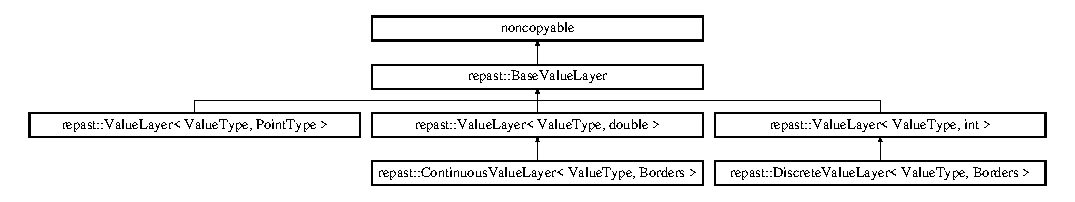
\includegraphics[height=2.269504cm]{classrepast_1_1_base_value_layer}
\end{center}
\end{figure}
\subsection*{Public Member Functions}
\begin{DoxyCompactItemize}
\item 
\hypertarget{classrepast_1_1_base_value_layer_a7b3e7be23a249233d40b2a72fa24e09f}{\hyperlink{classrepast_1_1_base_value_layer_a7b3e7be23a249233d40b2a72fa24e09f}{Base\-Value\-Layer} (const std\-::string \&\hyperlink{classrepast_1_1_base_value_layer_a27277765ee50f9d5446b253f77797f5c}{name})}\label{classrepast_1_1_base_value_layer_a7b3e7be23a249233d40b2a72fa24e09f}

\begin{DoxyCompactList}\small\item\em Creates a \hyperlink{classrepast_1_1_base_value_layer}{Base\-Value\-Layer} with the specified name. \end{DoxyCompactList}\item 
std\-::string \hyperlink{classrepast_1_1_base_value_layer_a27277765ee50f9d5446b253f77797f5c}{name} () const 
\begin{DoxyCompactList}\small\item\em Gets the value layer's name. \end{DoxyCompactList}\end{DoxyCompactItemize}
\subsection*{Protected Attributes}
\begin{DoxyCompactItemize}
\item 
\hypertarget{classrepast_1_1_base_value_layer_a1d85b694a3742262faaad8c5f513fd2f}{std\-::string {\bfseries \-\_\-name}}\label{classrepast_1_1_base_value_layer_a1d85b694a3742262faaad8c5f513fd2f}

\end{DoxyCompactItemize}


\subsection{Detailed Description}
Base implementation of a \hyperlink{classrepast_1_1_value_layer}{Value\-Layer}. 

A \hyperlink{classrepast_1_1_value_layer}{Value\-Layer} stores values by location. 

\subsection{Member Function Documentation}
\hypertarget{classrepast_1_1_base_value_layer_a27277765ee50f9d5446b253f77797f5c}{\index{repast\-::\-Base\-Value\-Layer@{repast\-::\-Base\-Value\-Layer}!name@{name}}
\index{name@{name}!repast::BaseValueLayer@{repast\-::\-Base\-Value\-Layer}}
\subsubsection[{name}]{\setlength{\rightskip}{0pt plus 5cm}std\-::string repast\-::\-Base\-Value\-Layer\-::name (
\begin{DoxyParamCaption}
{}
\end{DoxyParamCaption}
) const\hspace{0.3cm}{\ttfamily [inline]}}}\label{classrepast_1_1_base_value_layer_a27277765ee50f9d5446b253f77797f5c}


Gets the value layer's name. 

\begin{DoxyReturn}{Returns}
the name of the value layer. 
\end{DoxyReturn}


The documentation for this class was generated from the following files\-:\begin{DoxyCompactItemize}
\item 
repast\-\_\-hpc/Value\-Layer.\-h\item 
repast\-\_\-hpc/Value\-Layer.\-cpp\end{DoxyCompactItemize}

\hypertarget{classrepast_1_1_borders}{\section{repast\-:\-:Borders Class Reference}
\label{classrepast_1_1_borders}\index{repast\-::\-Borders@{repast\-::\-Borders}}
}


Base class for representations of border semantics (e.\-g.  




{\ttfamily \#include $<$Grid\-Components.\-h$>$}

Inheritance diagram for repast\-:\-:Borders\-:\begin{figure}[H]
\begin{center}
\leavevmode
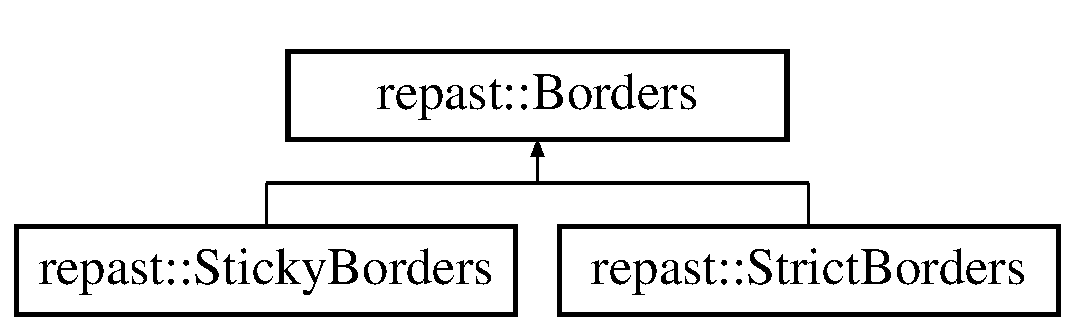
\includegraphics[height=2.000000cm]{classrepast_1_1_borders}
\end{center}
\end{figure}
\subsection*{Public Member Functions}
\begin{DoxyCompactItemize}
\item 
\hypertarget{classrepast_1_1_borders_ac8b1f8a3e7fed24eb7b6b301decaf704}{{\bfseries Borders} (\hyperlink{classrepast_1_1_grid_dimensions}{Grid\-Dimensions} d)}\label{classrepast_1_1_borders_ac8b1f8a3e7fed24eb7b6b301decaf704}

\item 
\hypertarget{classrepast_1_1_borders_a715ad00551f06f2f142fc40c5bfd711b}{void {\bfseries transform} (const std\-::vector$<$ int $>$ \&in, std\-::vector$<$ int $>$ \&out) const }\label{classrepast_1_1_borders_a715ad00551f06f2f142fc40c5bfd711b}

\item 
\hypertarget{classrepast_1_1_borders_a7400f48ce654bd8d88dde402b47a3e83}{void {\bfseries transform} (const std\-::vector$<$ double $>$ \&in, std\-::vector$<$ double $>$ \&out) const }\label{classrepast_1_1_borders_a7400f48ce654bd8d88dde402b47a3e83}

\item 
\hypertarget{classrepast_1_1_borders_af6602977a69a27b46e71ca8da5aeb259}{bool {\bfseries is\-Periodic} () const }\label{classrepast_1_1_borders_af6602977a69a27b46e71ca8da5aeb259}

\end{DoxyCompactItemize}
\subsection*{Protected Member Functions}
\begin{DoxyCompactItemize}
\item 
\hypertarget{classrepast_1_1_borders_a66336724557f7040d1240b771be1362a}{void {\bfseries bounds\-Check} (const std\-::vector$<$ int $>$ \&pt) const }\label{classrepast_1_1_borders_a66336724557f7040d1240b771be1362a}

\item 
\hypertarget{classrepast_1_1_borders_a9e364b71465c459a638551c40653440a}{void {\bfseries bounds\-Check} (const std\-::vector$<$ double $>$ \&pt) const }\label{classrepast_1_1_borders_a9e364b71465c459a638551c40653440a}

\end{DoxyCompactItemize}
\subsection*{Protected Attributes}
\begin{DoxyCompactItemize}
\item 
\hypertarget{classrepast_1_1_borders_a1e0e3961f4312901cd1c4909d6647cea}{const \hyperlink{classrepast_1_1_grid_dimensions}{Grid\-Dimensions} {\bfseries \-\_\-dimensions}}\label{classrepast_1_1_borders_a1e0e3961f4312901cd1c4909d6647cea}

\end{DoxyCompactItemize}


\subsection{Detailed Description}
Base class for representations of border semantics (e.\-g. 

Strict, Sticky, etc.) 

The documentation for this class was generated from the following files\-:\begin{DoxyCompactItemize}
\item 
repast\-\_\-hpc/Grid\-Components.\-h\item 
repast\-\_\-hpc/Grid\-Components.\-cpp\end{DoxyCompactItemize}

\hypertarget{classrepast_1_1_cart_topology}{\section{repast\-:\-:Cart\-Topology Class Reference}
\label{classrepast_1_1_cart_topology}\index{repast\-::\-Cart\-Topology@{repast\-::\-Cart\-Topology}}
}


Allows retrieval of the position of this process within the M\-P\-I Cartesian Topology into which it is placed.  




{\ttfamily \#include $<$Shared\-Base\-Grid.\-h$>$}

\subsection*{Public Member Functions}
\begin{DoxyCompactItemize}
\item 
\hypertarget{classrepast_1_1_cart_topology_ac6f5ad2d1539e6e9c5c4f905bd544c19}{{\bfseries Cart\-Topology} (std\-::vector$<$ int $>$ processes\-Per\-Dim, std\-::vector$<$ double $>$ origin, std\-::vector$<$ double $>$ extents, bool space\-Is\-Periodic, boost\-::mpi\-::communicator $\ast$world)}\label{classrepast_1_1_cart_topology_ac6f5ad2d1539e6e9c5c4f905bd544c19}

\item 
\hypertarget{classrepast_1_1_cart_topology_a7de71d6717688fcf67fd89409adeef90}{void \hyperlink{classrepast_1_1_cart_topology_a7de71d6717688fcf67fd89409adeef90}{get\-Coordinates} (int rank, std\-::vector$<$ int $>$ \&coords)}\label{classrepast_1_1_cart_topology_a7de71d6717688fcf67fd89409adeef90}

\begin{DoxyCompactList}\small\item\em Gets the coordinates in the M\-P\-I Cartesian Communicator for the specified rank. \end{DoxyCompactList}\item 
\hypertarget{classrepast_1_1_cart_topology_ac8e09a16688adc47670c082da1102b10}{\hyperlink{classrepast_1_1_grid_dimensions}{Grid\-Dimensions} \hyperlink{classrepast_1_1_cart_topology_ac8e09a16688adc47670c082da1102b10}{get\-Dimensions} (int rank)}\label{classrepast_1_1_cart_topology_ac8e09a16688adc47670c082da1102b10}

\begin{DoxyCompactList}\small\item\em Gets the \hyperlink{classrepast_1_1_grid_dimensions}{Grid\-Dimensions} boundaries for the specified rank. \end{DoxyCompactList}\item 
\hypertarget{classrepast_1_1_cart_topology_ac55a1b28941bedb6743c7a4977bdcea9}{\hyperlink{classrepast_1_1_grid_dimensions}{Grid\-Dimensions} \hyperlink{classrepast_1_1_cart_topology_ac55a1b28941bedb6743c7a4977bdcea9}{get\-Dimensions} (std\-::vector$<$ int $>$ \&p\-Coordinates)}\label{classrepast_1_1_cart_topology_ac55a1b28941bedb6743c7a4977bdcea9}

\begin{DoxyCompactList}\small\item\em Gets the \hyperlink{classrepast_1_1_grid_dimensions}{Grid\-Dimensions} boundaries for the specified M\-P\-I coordinates. \end{DoxyCompactList}\item 
\hypertarget{classrepast_1_1_cart_topology_adaedba511dc2fad8824ef1f64e9f073c}{void {\bfseries create\-Neighbors} (\hyperlink{classrepast_1_1_neighbors}{Neighbors} \&nghs)}\label{classrepast_1_1_cart_topology_adaedba511dc2fad8824ef1f64e9f073c}

\end{DoxyCompactItemize}


\subsection{Detailed Description}
Allows retrieval of the position of this process within the M\-P\-I Cartesian Topology into which it is placed. 

The documentation for this class was generated from the following files\-:\begin{DoxyCompactItemize}
\item 
repast\-\_\-hpc/Shared\-Base\-Grid.\-h\item 
repast\-\_\-hpc/Shared\-Base\-Grid.\-cpp\end{DoxyCompactItemize}

\hypertarget{classrepast_1_1_cell_contents}{\section{repast\-:\-:Cell\-Contents$<$ Agent\-Content, G\-P\-Type $>$ Class Template Reference}
\label{classrepast_1_1_cell_contents}\index{repast\-::\-Cell\-Contents$<$ Agent\-Content, G\-P\-Type $>$@{repast\-::\-Cell\-Contents$<$ Agent\-Content, G\-P\-Type $>$}}
}


{\itshape D\-E\-P\-R\-E\-C\-A\-T\-E\-D} Encapsulates the contents of a grid / space location so that it can be sent between processes.  




{\ttfamily \#include $<$Shared\-Base\-Grid.\-h$>$}

\subsection*{Public Member Functions}
\begin{DoxyCompactItemize}
\item 
\hypertarget{classrepast_1_1_cell_contents_afbe0f0f9af0d4d9351be254522984db6}{{\footnotesize template$<$class Archive $>$ }\\void {\bfseries serialize} (Archive \&ar, const unsigned int version)}\label{classrepast_1_1_cell_contents_afbe0f0f9af0d4d9351be254522984db6}

\item 
\hypertarget{classrepast_1_1_cell_contents_afbd1679d216cdef051c0fc985327925f}{{\bfseries Cell\-Contents} (\hyperlink{classrepast_1_1_point}{Point}$<$ G\-P\-Type $>$ pt)}\label{classrepast_1_1_cell_contents_afbd1679d216cdef051c0fc985327925f}

\end{DoxyCompactItemize}
\subsection*{Public Attributes}
\begin{DoxyCompactItemize}
\item 
\hypertarget{classrepast_1_1_cell_contents_a77ce242dc0f59276008fdfb42a8db000}{\hyperlink{classrepast_1_1_point}{Point}$<$ G\-P\-Type $>$ {\bfseries \-\_\-pt}}\label{classrepast_1_1_cell_contents_a77ce242dc0f59276008fdfb42a8db000}

\item 
\hypertarget{classrepast_1_1_cell_contents_ad33d7bbe7d5b66190414d1e5e6791c50}{std\-::vector$<$ Agent\-Content $>$ {\bfseries \-\_\-objs}}\label{classrepast_1_1_cell_contents_ad33d7bbe7d5b66190414d1e5e6791c50}

\end{DoxyCompactItemize}
\subsection*{Friends}
\begin{DoxyCompactItemize}
\item 
\hypertarget{classrepast_1_1_cell_contents_ac98d07dd8f7b70e16ccb9a01abf56b9c}{class {\bfseries boost\-::serialization\-::access}}\label{classrepast_1_1_cell_contents_ac98d07dd8f7b70e16ccb9a01abf56b9c}

\end{DoxyCompactItemize}


\subsection{Detailed Description}
\subsubsection*{template$<$typename Agent\-Content, typename G\-P\-Type$>$class repast\-::\-Cell\-Contents$<$ Agent\-Content, G\-P\-Type $>$}

{\itshape D\-E\-P\-R\-E\-C\-A\-T\-E\-D} Encapsulates the contents of a grid / space location so that it can be sent between processes. 

\begin{DoxyRefDesc}{Deprecated}
\item[\hyperlink{deprecated__deprecated000001}{Deprecated}]Replaced by \hyperlink{classrepast_1_1_projection_info_packet}{Projection\-Info\-Packet} as of Version 2.\-0 \end{DoxyRefDesc}


The documentation for this class was generated from the following file\-:\begin{DoxyCompactItemize}
\item 
repast\-\_\-hpc/Shared\-Base\-Grid.\-h\end{DoxyCompactItemize}

\hypertarget{class_cerr_appender}{\section{Cerr\-Appender Class Reference}
\label{class_cerr_appender}\index{Cerr\-Appender@{Cerr\-Appender}}
}
Inheritance diagram for Cerr\-Appender\-:\begin{figure}[H]
\begin{center}
\leavevmode
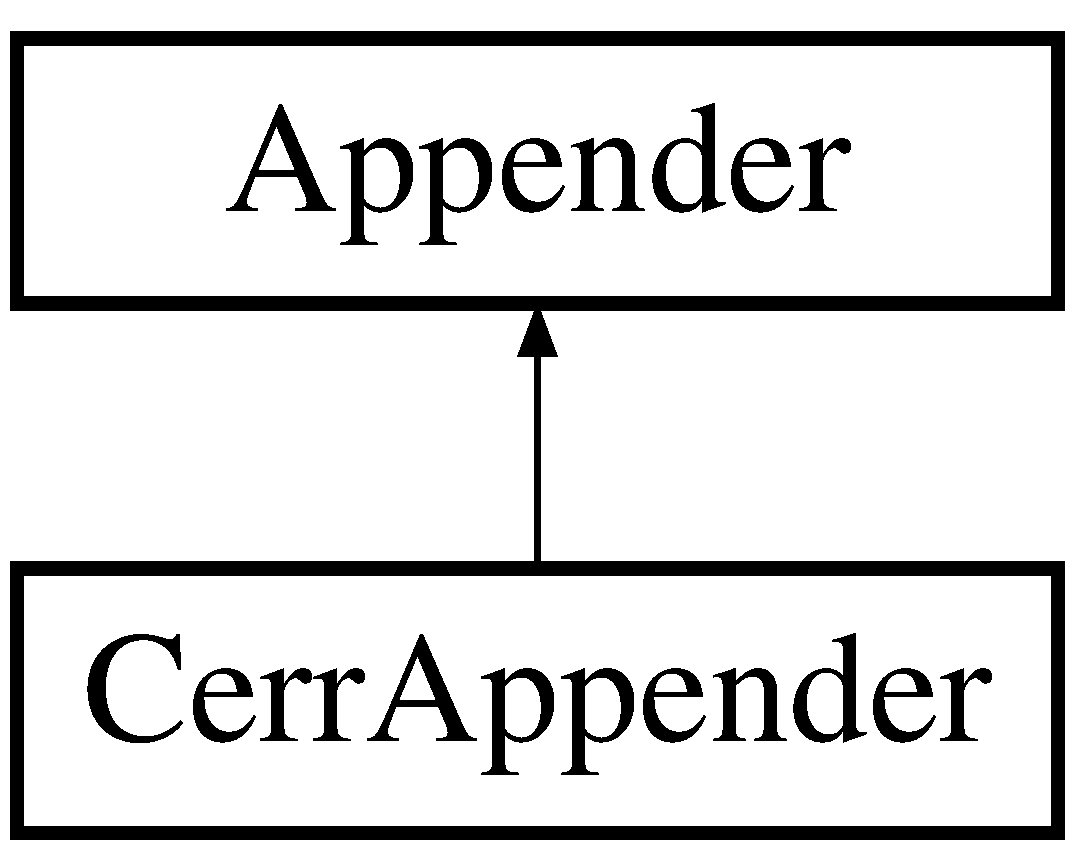
\includegraphics[height=2.000000cm]{class_cerr_appender}
\end{center}
\end{figure}
\subsection*{Public Member Functions}
\begin{DoxyCompactItemize}
\item 
\hypertarget{class_cerr_appender_a190f6e2f820f26bf51aa142eb746f041}{void {\bfseries write} (const string \&line)}\label{class_cerr_appender_a190f6e2f820f26bf51aa142eb746f041}

\end{DoxyCompactItemize}
\subsection*{Additional Inherited Members}


The documentation for this class was generated from the following file\-:\begin{DoxyCompactItemize}
\item 
repast\-\_\-hpc/logger.\-cpp\end{DoxyCompactItemize}

\hypertarget{class_config_lexer}{\section{Config\-Lexer Class Reference}
\label{class_config_lexer}\index{Config\-Lexer@{Config\-Lexer}}
}
\subsection*{Public Member Functions}
\begin{DoxyCompactItemize}
\item 
\hypertarget{class_config_lexer_a046cf2dcd1d747298665437b8b21ef11}{{\bfseries Config\-Lexer} (const string \&file\-\_\-name, boost\-::mpi\-::communicator $\ast$comm=0, int max\-Config\-File\-Size=M\-A\-X\-\_\-\-C\-O\-N\-F\-I\-G\-\_\-\-F\-I\-L\-E\-\_\-\-S\-I\-Z\-E)}\label{class_config_lexer_a046cf2dcd1d747298665437b8b21ef11}

\item 
\hypertarget{class_config_lexer_ac6c1e251c3db1f30c50b20b1ee7450f1}{T\-O\-K\-E\-N {\bfseries next\-\_\-token} ()}\label{class_config_lexer_ac6c1e251c3db1f30c50b20b1ee7450f1}

\item 
\hypertarget{class_config_lexer_adc9e9967c636a264708b3bf06aaf3a76}{string {\bfseries key} ()}\label{class_config_lexer_adc9e9967c636a264708b3bf06aaf3a76}

\item 
\hypertarget{class_config_lexer_abd3e04c84b9411f4232a2063fabdb6ac}{string {\bfseries value} ()}\label{class_config_lexer_abd3e04c84b9411f4232a2063fabdb6ac}

\item 
\hypertarget{class_config_lexer_a483c74b57e0ec56abdb815dc91511c51}{string {\bfseries error} ()}\label{class_config_lexer_a483c74b57e0ec56abdb815dc91511c51}

\item 
\hypertarget{class_config_lexer_adfa7ec76d67765cd52ff3c91af5f9dbd}{int {\bfseries line} ()}\label{class_config_lexer_adfa7ec76d67765cd52ff3c91af5f9dbd}

\item 
\hypertarget{class_config_lexer_a3f6909108d4b8f09b12f1c9332fc9930}{void {\bfseries reset} ()}\label{class_config_lexer_a3f6909108d4b8f09b12f1c9332fc9930}

\end{DoxyCompactItemize}


The documentation for this class was generated from the following file\-:\begin{DoxyCompactItemize}
\item 
repast\-\_\-hpc/logger.\-cpp\end{DoxyCompactItemize}

\hypertarget{classrepast_1_1_context}{\section{repast\-:\-:Context$<$ T $>$ Class Template Reference}
\label{classrepast_1_1_context}\index{repast\-::\-Context$<$ T $>$@{repast\-::\-Context$<$ T $>$}}
}


Collection of agents of type T with set semantics.  




{\ttfamily \#include $<$Context.\-h$>$}

Inheritance diagram for repast\-:\-:Context$<$ T $>$\-:\begin{figure}[H]
\begin{center}
\leavevmode
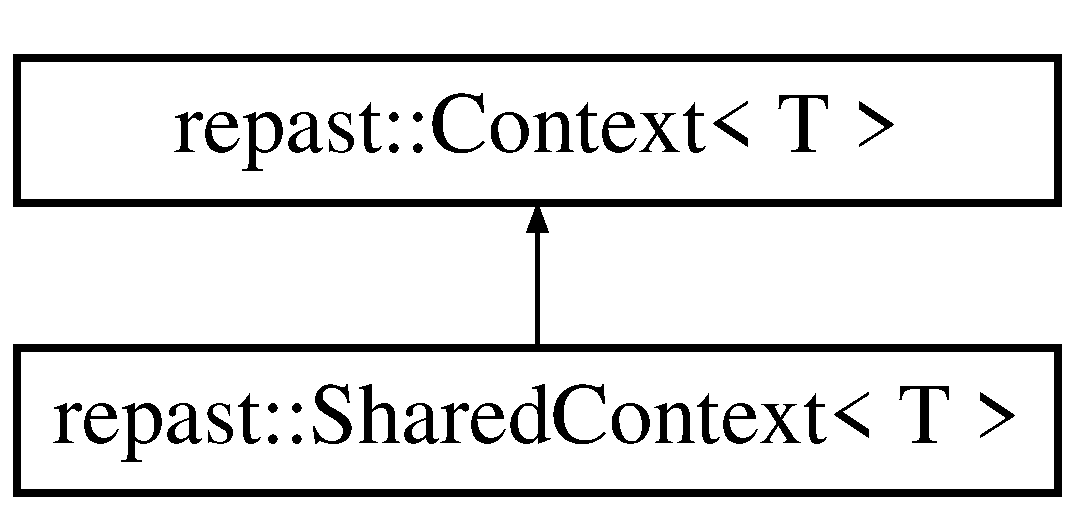
\includegraphics[height=2.000000cm]{classrepast_1_1_context}
\end{center}
\end{figure}
\subsection*{Public Types}
\begin{DoxyCompactItemize}
\item 
\hypertarget{classrepast_1_1_context_a94c26538a555d9d781034b89cfa1cc8a}{typedef \\*
boost\-::transform\-\_\-iterator\\*
$<$ \hyperlink{structrepast_1_1_second_element}{Second\-Element}$<$ T $>$, typename \\*
Agent\-Map\-::const\-\_\-iterator $>$ {\bfseries const\-\_\-iterator}}\label{classrepast_1_1_context_a94c26538a555d9d781034b89cfa1cc8a}

\item 
\hypertarget{classrepast_1_1_context_ac27ec9bbfb365044a5088e1cdedc3ad1}{typedef boost\-::filter\-\_\-iterator\\*
$<$ \hyperlink{structrepast_1_1_is_agent_type}{Is\-Agent\-Type}$<$ T $>$, typename \\*
\hyperlink{classrepast_1_1_context}{Context}$<$ T $>$\-::const\-\_\-iterator $>$ {\bfseries const\-\_\-bytype\-\_\-iterator}}\label{classrepast_1_1_context_ac27ec9bbfb365044a5088e1cdedc3ad1}

\end{DoxyCompactItemize}
\subsection*{Public Member Functions}
\begin{DoxyCompactItemize}
\item 
\hypertarget{classrepast_1_1_context_ab86028066396e40cc29cfff8d54ee581}{virtual \hyperlink{classrepast_1_1_context_ab86028066396e40cc29cfff8d54ee581}{$\sim$\-Context} ()}\label{classrepast_1_1_context_ab86028066396e40cc29cfff8d54ee581}

\begin{DoxyCompactList}\small\item\em Destroys this context and the projections it contains. \end{DoxyCompactList}\item 
T $\ast$ \hyperlink{classrepast_1_1_context_ad0bc4b142fe7154c03d4e4bd2f6836ed}{add\-Agent} (T $\ast$agent)
\begin{DoxyCompactList}\small\item\em Adds the agent to the context. \end{DoxyCompactList}\item 
virtual void \hyperlink{classrepast_1_1_context_a96d41e5246dc2940be3ea45f2a233487}{add\-Projection} (\hyperlink{classrepast_1_1_projection}{Projection}$<$ T $>$ $\ast$projection)
\begin{DoxyCompactList}\small\item\em Adds the specified projection to this context. \end{DoxyCompactList}\item 
\hyperlink{classrepast_1_1_projection}{Projection}$<$ T $>$ $\ast$ \hyperlink{classrepast_1_1_context_a10b60609163a2906e23d0b02bf76d7ac}{get\-Projection} (const std\-::string \&name)
\begin{DoxyCompactList}\small\item\em Get the named \hyperlink{classrepast_1_1_projection}{Projection}. \end{DoxyCompactList}\item 
void \hyperlink{classrepast_1_1_context_a7ef4c1e4a5f789b6402574fb2d8bd8ef}{remove\-Agent} (const \hyperlink{classrepast_1_1_agent_id}{Agent\-Id} id)
\begin{DoxyCompactList}\small\item\em Removes the specified agent from this context. \end{DoxyCompactList}\item 
\hypertarget{classrepast_1_1_context_a1ad64ba451c47e2364f33e73b482a3a4}{void \hyperlink{classrepast_1_1_context_a1ad64ba451c47e2364f33e73b482a3a4}{remove\-Agent} (T $\ast$agent)}\label{classrepast_1_1_context_a1ad64ba451c47e2364f33e73b482a3a4}

\begin{DoxyCompactList}\small\item\em Removes the specified agent from this context. \end{DoxyCompactList}\item 
T $\ast$ \hyperlink{classrepast_1_1_context_a72ec330f6e930b4c83929a70df993b43}{get\-Agent} (const \hyperlink{classrepast_1_1_agent_id}{Agent\-Id} \&id)
\begin{DoxyCompactList}\small\item\em Gets the specified agent. \end{DoxyCompactList}\item 
void \hyperlink{classrepast_1_1_context_a543dcc0f3ea4ecbe054232eaaa9c72e4}{get\-Random\-Agents} (const int count, std\-::vector$<$ T $\ast$ $>$ \&agents)
\begin{DoxyCompactList}\small\item\em Gets at random the specified count of agents and returns them in the agents vector. \end{DoxyCompactList}\item 
const\-\_\-iterator \hyperlink{classrepast_1_1_context_a0c69277c868b42ee0bb0d3b90a1df46d}{begin} () const 
\begin{DoxyCompactList}\small\item\em Gets the start of iterator over the agents in this context. \end{DoxyCompactList}\item 
const\-\_\-iterator \hyperlink{classrepast_1_1_context_af584236067222d8c1a2aa51b5e396da4}{end} () const 
\begin{DoxyCompactList}\small\item\em Gets the end of an iterator over the agents in this context. \end{DoxyCompactList}\item 
const\-\_\-bytype\-\_\-iterator \hyperlink{classrepast_1_1_context_a2b77a55622dcdce4b82e8c2864642544}{by\-Type\-Begin} (int type\-Id) const 
\begin{DoxyCompactList}\small\item\em Gets the start of an iterator over agents in this context of the specified type. \end{DoxyCompactList}\item 
const\-\_\-bytype\-\_\-iterator \hyperlink{classrepast_1_1_context_aa7e427063cdbfc5e37764291df2b2b53}{by\-Type\-End} (int type\-Id) const 
\begin{DoxyCompactList}\small\item\em Gets the end of an iterator over agents in this context of the specified type. \end{DoxyCompactList}\item 
\hypertarget{classrepast_1_1_context_a579cde2d1318e073f9fd068a7b0ed1a5}{bool \hyperlink{classrepast_1_1_context_a579cde2d1318e073f9fd068a7b0ed1a5}{contains} (const \hyperlink{classrepast_1_1_agent_id}{Agent\-Id} \&id)}\label{classrepast_1_1_context_a579cde2d1318e073f9fd068a7b0ed1a5}

\begin{DoxyCompactList}\small\item\em Returns true if the specified agent is in this context, otherwise false. \end{DoxyCompactList}\item 
\hypertarget{classrepast_1_1_context_aa86fbff836e4066f98c893157c76db88}{int \hyperlink{classrepast_1_1_context_aa86fbff836e4066f98c893157c76db88}{size} () const }\label{classrepast_1_1_context_aa86fbff836e4066f98c893157c76db88}

\begin{DoxyCompactList}\small\item\em Gets the size (number of agents) in this context. \end{DoxyCompactList}\item 
void \hyperlink{classrepast_1_1_context_a9120a6aac361baa92d6dbd83410ff576}{add\-Value\-Layer} (\hyperlink{classrepast_1_1_base_value_layer}{Base\-Value\-Layer} $\ast$value\-Layer)
\begin{DoxyCompactList}\small\item\em Adds a value layer to this context. \end{DoxyCompactList}\item 
{\footnotesize template$<$typename Value\-Type , typename Borders $>$ }\\\hyperlink{classrepast_1_1_discrete_value_layer}{Discrete\-Value\-Layer}$<$ Value\-Type, \\*
\hyperlink{classrepast_1_1_borders}{Borders} $>$ $\ast$ \hyperlink{classrepast_1_1_context_ac4e06221e76065ae8ee50815bb1a7a41}{get\-Discrete\-Value\-Layer} (const std\-::string \&value\-Layer\-Name)
\begin{DoxyCompactList}\small\item\em Gets the named discrete value layer from this \hyperlink{classrepast_1_1_context}{Context}. \end{DoxyCompactList}\item 
{\footnotesize template$<$typename Value\-Type , typename Borders $>$ }\\\hyperlink{classrepast_1_1_continuous_value_layer}{Continuous\-Value\-Layer}\\*
$<$ Value\-Type, \hyperlink{classrepast_1_1_borders}{Borders} $>$ $\ast$ \hyperlink{classrepast_1_1_context_a9ac760826f1f535b474af50dec727e9f}{get\-Continuous\-Value\-Layer} (const std\-::string \&value\-Layer\-Name)
\begin{DoxyCompactList}\small\item\em Gets the named continuous value layer from this \hyperlink{classrepast_1_1_context}{Context}. \end{DoxyCompactList}\item 
{\footnotesize template$<$typename filter\-Struct $>$ }\\boost\-::filter\-\_\-iterator\\*
$<$ filter\-Struct, typename \\*
\hyperlink{classrepast_1_1_context}{Context}$<$ T $>$\-::const\-\_\-iterator $>$ \hyperlink{classrepast_1_1_context_ab54a094afb5834a34be46e732465ff30}{filtered\-Begin} (const filter\-Struct \&f\-Struct)
\begin{DoxyCompactList}\small\item\em Creates a filtered iterator over the set of agents in this context and returns it with a value equal to the beginning of the list. \end{DoxyCompactList}\item 
{\footnotesize template$<$typename filter\-Struct $>$ }\\boost\-::filter\-\_\-iterator\\*
$<$ filter\-Struct, typename \\*
\hyperlink{classrepast_1_1_context}{Context}$<$ T $>$\-::const\-\_\-iterator $>$ \hyperlink{classrepast_1_1_context_ad12bb3d7e2578bf80ebbd0dd1b1a7ebd}{filtered\-End} (const filter\-Struct \&f\-Struct)
\begin{DoxyCompactList}\small\item\em Creates a filtered iterator over the set of agents in this context and returns it with a value equal to one step past end of the list. \end{DoxyCompactList}\item 
{\footnotesize template$<$typename filter\-Struct $>$ }\\boost\-::filter\-\_\-iterator\\*
$<$ filter\-Struct, typename \\*
\hyperlink{classrepast_1_1_context}{Context}$<$ T $>$\\*
\-::const\-\_\-bytype\-\_\-iterator $>$ \hyperlink{classrepast_1_1_context_aa7abe8aefbda43b0b35fcbd3589b465c}{by\-Type\-Filtered\-Begin} (const int type, const filter\-Struct \&f\-Struct)
\begin{DoxyCompactList}\small\item\em Creates a filtered iterator over the set of agents in this context of the specified type (per their \hyperlink{classrepast_1_1_agent_id}{Agent\-Id} values), and returns it with a value equal to the beginning of the list. \end{DoxyCompactList}\item 
{\footnotesize template$<$typename filter\-Struct $>$ }\\boost\-::filter\-\_\-iterator\\*
$<$ filter\-Struct, typename \\*
\hyperlink{classrepast_1_1_context}{Context}$<$ T $>$\\*
\-::const\-\_\-bytype\-\_\-iterator $>$ \hyperlink{classrepast_1_1_context_a94cee2bd8c4325a7fe79048c0f12a5b6}{by\-Type\-Filtered\-End} (const int type, const filter\-Struct \&f\-Struct)
\begin{DoxyCompactList}\small\item\em Creates a filtered iterator over the set of agents in this context of the specified type (per their \hyperlink{classrepast_1_1_agent_id}{Agent\-Id} values), and returns it with a value equal to one past the end of the list. \end{DoxyCompactList}\item 
void \hyperlink{classrepast_1_1_context_a6f389ebd5bea672d5d7d14ffba5b710f}{select\-Agents} (std\-::set$<$ T $\ast$ $>$ \&selected\-Agents, bool remove=false)
\begin{DoxyCompactList}\small\item\em Gets a set of pointers to all agents in this context. \end{DoxyCompactList}\item 
void \hyperlink{classrepast_1_1_context_aacc9180a8ff5e079ca37edb08a434ff9}{select\-Agents} (std\-::vector$<$ T $\ast$ $>$ \&selected\-Agents, bool remove=false)
\begin{DoxyCompactList}\small\item\em Gets a randomly ordered vector of pointers to all agents in this context. \end{DoxyCompactList}\item 
void \hyperlink{classrepast_1_1_context_a305bd5cfc509be346842567fdf72f97d}{select\-Agents} (int count, std\-::set$<$ T $\ast$ $>$ \&selected\-Agents, bool remove=false)
\begin{DoxyCompactList}\small\item\em Gets a set of pointers to a specified number of randomly selected agents. \end{DoxyCompactList}\item 
void \hyperlink{classrepast_1_1_context_acba9351838355a0cfe3dff074448bbc5}{select\-Agents} (int count, std\-::vector$<$ T $\ast$ $>$ \&selected\-Agents, bool remove=false)
\begin{DoxyCompactList}\small\item\em Gets a randomly ordered vector of pointers to a specified number of randomly selected agents. \end{DoxyCompactList}\item 
void \hyperlink{classrepast_1_1_context_abf2012f09fb75bfdeb798431e63edfde}{select\-Agents} (std\-::set$<$ T $\ast$ $>$ \&selected\-Agents, int type, bool remove=false, int pop\-Size=-\/1)
\begin{DoxyCompactList}\small\item\em Gets a set of pointers to all agents in this context of a specified type (per their \hyperlink{classrepast_1_1_agent_id}{Agent\-Id} values). \end{DoxyCompactList}\item 
void \hyperlink{classrepast_1_1_context_af8ca3deb5e820bf84df1dd83fdd14f2d}{select\-Agents} (std\-::vector$<$ T $\ast$ $>$ \&selected\-Agents, int type, bool remove=false, int pop\-Size=-\/1)
\begin{DoxyCompactList}\small\item\em Gets a randomly ordered vector of pointers to all agents in this context of a specified type (per their \hyperlink{classrepast_1_1_agent_id}{Agent\-Id} values). \end{DoxyCompactList}\item 
void \hyperlink{classrepast_1_1_context_a8961d3bd4575afac3ef571166739ac39}{select\-Agents} (int count, std\-::set$<$ T $\ast$ $>$ \&selected\-Agents, int type, bool remove=false, int pop\-Size=-\/1)
\begin{DoxyCompactList}\small\item\em Gets a set of pointers to a specified number of randomly selected agents of a specified type (per their \hyperlink{classrepast_1_1_agent_id}{Agent\-Id} values). \end{DoxyCompactList}\item 
void \hyperlink{classrepast_1_1_context_aae94abf702a7223aaadc74da4f1fd639}{select\-Agents} (int count, std\-::vector$<$ T $\ast$ $>$ \&selected\-Agents, int type, bool remove=false, int pop\-Size=-\/1)
\begin{DoxyCompactList}\small\item\em Gets a randomly ordered vector of pointers to a specified number of randomly selected agents of a specified type (per their \hyperlink{classrepast_1_1_agent_id}{Agent\-Id} values). \end{DoxyCompactList}\item 
{\footnotesize template$<$typename filter\-Struct $>$ }\\void \hyperlink{classrepast_1_1_context_a926168c2e765e58473d901f56a6a42f7}{select\-Agents} (std\-::set$<$ T $\ast$ $>$ \&selected\-Agents, filter\-Struct \&filter, bool remove=false, int pop\-Size=-\/1)
\begin{DoxyCompactList}\small\item\em Gets a set of pointers to all agents in this context matching a user-\/defined filter. \end{DoxyCompactList}\item 
{\footnotesize template$<$typename filter\-Struct $>$ }\\void \hyperlink{classrepast_1_1_context_a5011ce09dc44040c235b176261defcf3}{select\-Agents} (std\-::vector$<$ T $\ast$ $>$ \&selected\-Agents, filter\-Struct \&filter, bool remove=false, int pop\-Size=-\/1)
\begin{DoxyCompactList}\small\item\em Gets a randomly ordered vector of pointers to all agents in this context matching a user-\/defined filter. \end{DoxyCompactList}\item 
{\footnotesize template$<$typename filter\-Struct $>$ }\\void \hyperlink{classrepast_1_1_context_a10218ffcf74884be4e12c49a26106878}{select\-Agents} (int count, std\-::set$<$ T $\ast$ $>$ \&selected\-Agents, filter\-Struct \&filter, bool remove=false, int pop\-Size=-\/1)
\begin{DoxyCompactList}\small\item\em Gets a set of pointers to a specified number of randomly selected agents matching a user-\/defined filter. \end{DoxyCompactList}\item 
{\footnotesize template$<$typename filter\-Struct $>$ }\\void \hyperlink{classrepast_1_1_context_a41673cd1e0623849d505884afaaf2581}{select\-Agents} (int count, std\-::vector$<$ T $\ast$ $>$ \&selected\-Agents, filter\-Struct \&filter, bool remove=false, int pop\-Size=-\/1)
\begin{DoxyCompactList}\small\item\em Gets a randomly ordered vector of pointers to a specified number of randomly selected agents matching a user-\/defined filter. \end{DoxyCompactList}\item 
{\footnotesize template$<$typename filter\-Struct $>$ }\\void \hyperlink{classrepast_1_1_context_a2d678fd5e8a320db144d17fb863ee91a}{select\-Agents} (std\-::set$<$ T $\ast$ $>$ \&selected\-Agents, int type, filter\-Struct \&filter, bool remove=false, int pop\-Size=-\/1)
\begin{DoxyCompactList}\small\item\em Gets a set of pointers to all agents in this context of a specified type (per their \hyperlink{classrepast_1_1_agent_id}{Agent\-Id} values) and matching a user-\/defined filter. \end{DoxyCompactList}\item 
{\footnotesize template$<$typename filter\-Struct $>$ }\\void \hyperlink{classrepast_1_1_context_a07cf00b1c5a00b676c5de83e8db438aa}{select\-Agents} (std\-::vector$<$ T $\ast$ $>$ \&selected\-Agents, int type, filter\-Struct \&filter, bool remove=false, int pop\-Size=-\/1)
\begin{DoxyCompactList}\small\item\em Gets a randomly ordered vector of pointers to all agents in this context of a specified type (per their \hyperlink{classrepast_1_1_agent_id}{Agent\-Id} values) and matching a user-\/defined filter. \end{DoxyCompactList}\item 
{\footnotesize template$<$typename filter\-Struct $>$ }\\void \hyperlink{classrepast_1_1_context_afe8f496266275c9edb065c06c6574fc1}{select\-Agents} (int count, std\-::set$<$ T $\ast$ $>$ \&selected\-Agents, int type, filter\-Struct \&filter, bool remove=false, int pop\-Size=-\/1)
\begin{DoxyCompactList}\small\item\em Gets a set of pointers to a specified number of randomly selected agents of a specified type (per their \hyperlink{classrepast_1_1_agent_id}{Agent\-Id} values) and matching a user-\/defined filter. \end{DoxyCompactList}\item 
{\footnotesize template$<$typename filter\-Struct $>$ }\\void \hyperlink{classrepast_1_1_context_ab4aea4be7eaf1c4be741a371e90057a9}{select\-Agents} (int count, std\-::vector$<$ T $\ast$ $>$ \&selected\-Agents, int type, filter\-Struct \&filter, bool remove=false, int pop\-Size=-\/1)
\begin{DoxyCompactList}\small\item\em Gets a randomly ordered vector of pointers to a specified number of randomly selected agents of a specified type (per their \hyperlink{classrepast_1_1_agent_id}{Agent\-Id} values) and matching a user-\/defined filter. \end{DoxyCompactList}\item 
void \hyperlink{classrepast_1_1_context_a8a420350cd434f4e0f30a3d41c93298f}{get\-Projection\-Info} (\hyperlink{classrepast_1_1_agent_request}{Agent\-Request} req, std\-::map$<$ std\-::string, std\-::vector$<$ \hyperlink{classrepast_1_1_projection_info_packet}{repast\-::\-Projection\-Info\-Packet} $\ast$ $>$ $>$ \&map, bool secondary\-Info=false, std\-::set$<$ \hyperlink{classrepast_1_1_agent_id}{Agent\-Id} $>$ $\ast$secondary\-Ids=0, int dest\-Proc=-\/1)
\begin{DoxyCompactList}\small\item\em Gets the projection information for all projections in this context, for all agents whose I\-Ds are listed in the \hyperlink{classrepast_1_1_agent_request}{Agent\-Request}. \end{DoxyCompactList}\item 
void \hyperlink{classrepast_1_1_context_a9470dbe20a0b4243d52edea86c213feb}{set\-Projection\-Info} (std\-::map$<$ std\-::string, std\-::vector$<$ \hyperlink{classrepast_1_1_projection_info_packet}{repast\-::\-Projection\-Info\-Packet} $\ast$ $>$ $>$ \&proj\-Info)
\begin{DoxyCompactList}\small\item\em Sets the projection information as specified. \end{DoxyCompactList}\item 
\hypertarget{classrepast_1_1_context_a88097fca27376b1fc460bb75f47869bb}{void {\bfseries clean\-Projection\-Info} (std\-::set$<$ \hyperlink{classrepast_1_1_agent_id}{Agent\-Id} $>$ \&agents\-To\-Keep)}\label{classrepast_1_1_context_a88097fca27376b1fc460bb75f47869bb}

\end{DoxyCompactItemize}
\subsection*{Protected Attributes}
\begin{DoxyCompactItemize}
\item 
\hypertarget{classrepast_1_1_context_aed0c509cff2035ca99c2b2fc299dcca0}{std\-::vector$<$ \hyperlink{classrepast_1_1_projection}{Projection}$<$ T $>$ $\ast$ $>$ {\bfseries projections}}\label{classrepast_1_1_context_aed0c509cff2035ca99c2b2fc299dcca0}

\end{DoxyCompactItemize}


\subsection{Detailed Description}
\subsubsection*{template$<$typename T$>$class repast\-::\-Context$<$ T $>$}

Collection of agents of type T with set semantics. 

Object identity and equality is determined by their \hyperlink{classrepast_1_1_agent_id}{Agent\-Id}.


\begin{DoxyTemplParams}{Template Parameters}
{\em the} & type objects contained by the \hyperlink{classrepast_1_1_context}{Context}. The T must extends \hyperlink{classrepast_1_1_agent}{repast\-::\-Agent}. \\
\hline
\end{DoxyTemplParams}


\subsection{Member Function Documentation}
\hypertarget{classrepast_1_1_context_ad0bc4b142fe7154c03d4e4bd2f6836ed}{\index{repast\-::\-Context@{repast\-::\-Context}!add\-Agent@{add\-Agent}}
\index{add\-Agent@{add\-Agent}!repast::Context@{repast\-::\-Context}}
\subsubsection[{add\-Agent}]{\setlength{\rightskip}{0pt plus 5cm}template$<$typename T $>$ T $\ast$ {\bf repast\-::\-Context}$<$ T $>$\-::add\-Agent (
\begin{DoxyParamCaption}
\item[{T $\ast$}]{agent}
\end{DoxyParamCaption}
)}}\label{classrepast_1_1_context_ad0bc4b142fe7154c03d4e4bd2f6836ed}


Adds the agent to the context. 

Performs a check to ensure that no agent with the same I\-D (presumably the 'same' agent) has previously been added. If a matching I\-D is found, the new agent is not added, and the address of the pre-\/existing agent is returned. If no match is found, the agent is added and the return value is the same as the value passed


\begin{DoxyParams}{Parameters}
{\em agent} & the agent to add\\
\hline
\end{DoxyParams}
\begin{DoxyReturn}{Returns}
the address of the agent in the context; will be the same as the address passed if the agent was successfully added, but if there was already an agent with the same I\-D the address returned will be that of the pre-\/existing agent, which is not replaced. 
\end{DoxyReturn}
\hypertarget{classrepast_1_1_context_a96d41e5246dc2940be3ea45f2a233487}{\index{repast\-::\-Context@{repast\-::\-Context}!add\-Projection@{add\-Projection}}
\index{add\-Projection@{add\-Projection}!repast::Context@{repast\-::\-Context}}
\subsubsection[{add\-Projection}]{\setlength{\rightskip}{0pt plus 5cm}template$<$typename T $>$ void {\bf repast\-::\-Context}$<$ T $>$\-::add\-Projection (
\begin{DoxyParamCaption}
\item[{{\bf Projection}$<$ T $>$ $\ast$}]{projection}
\end{DoxyParamCaption}
)\hspace{0.3cm}{\ttfamily [virtual]}}}\label{classrepast_1_1_context_a96d41e5246dc2940be3ea45f2a233487}


Adds the specified projection to this context. 

All the agents in this context will be added to the \hyperlink{classrepast_1_1_projection}{Projection}. Any agents subsequently added to this context will also be added to the \hyperlink{classrepast_1_1_projection}{Projection}.


\begin{DoxyParams}{Parameters}
{\em projection} & the projection to add \\
\hline
\end{DoxyParams}


Reimplemented in \hyperlink{classrepast_1_1_shared_context_af8f235d4d8e4b1efc548ea8a5b1ab75d}{repast\-::\-Shared\-Context$<$ T $>$}.

\hypertarget{classrepast_1_1_context_a9120a6aac361baa92d6dbd83410ff576}{\index{repast\-::\-Context@{repast\-::\-Context}!add\-Value\-Layer@{add\-Value\-Layer}}
\index{add\-Value\-Layer@{add\-Value\-Layer}!repast::Context@{repast\-::\-Context}}
\subsubsection[{add\-Value\-Layer}]{\setlength{\rightskip}{0pt plus 5cm}template$<$typename T $>$ void {\bf repast\-::\-Context}$<$ T $>$\-::add\-Value\-Layer (
\begin{DoxyParamCaption}
\item[{{\bf Base\-Value\-Layer} $\ast$}]{value\-Layer}
\end{DoxyParamCaption}
)}}\label{classrepast_1_1_context_a9120a6aac361baa92d6dbd83410ff576}


Adds a value layer to this context. 


\begin{DoxyParams}{Parameters}
{\em value\-Layer} & the value layer to add \\
\hline
\end{DoxyParams}
\hypertarget{classrepast_1_1_context_a0c69277c868b42ee0bb0d3b90a1df46d}{\index{repast\-::\-Context@{repast\-::\-Context}!begin@{begin}}
\index{begin@{begin}!repast::Context@{repast\-::\-Context}}
\subsubsection[{begin}]{\setlength{\rightskip}{0pt plus 5cm}template$<$typename T$>$ const\-\_\-iterator {\bf repast\-::\-Context}$<$ T $>$\-::begin (
\begin{DoxyParamCaption}
{}
\end{DoxyParamCaption}
) const\hspace{0.3cm}{\ttfamily [inline]}}}\label{classrepast_1_1_context_a0c69277c868b42ee0bb0d3b90a1df46d}


Gets the start of iterator over the agents in this context. 

The iterator derefrences into shared\-\_\-ptr$<$\-T$>$. The actual agent can be accessed by derefrenceing the iter\-: ($\ast$iter)-\/$>$get\-Id() for example.

\begin{DoxyReturn}{Returns}
the start of iterator over the agents in this context. 
\end{DoxyReturn}
\hypertarget{classrepast_1_1_context_a2b77a55622dcdce4b82e8c2864642544}{\index{repast\-::\-Context@{repast\-::\-Context}!by\-Type\-Begin@{by\-Type\-Begin}}
\index{by\-Type\-Begin@{by\-Type\-Begin}!repast::Context@{repast\-::\-Context}}
\subsubsection[{by\-Type\-Begin}]{\setlength{\rightskip}{0pt plus 5cm}template$<$typename T$>$ const\-\_\-bytype\-\_\-iterator {\bf repast\-::\-Context}$<$ T $>$\-::by\-Type\-Begin (
\begin{DoxyParamCaption}
\item[{int}]{type\-Id}
\end{DoxyParamCaption}
) const\hspace{0.3cm}{\ttfamily [inline]}}}\label{classrepast_1_1_context_a2b77a55622dcdce4b82e8c2864642544}


Gets the start of an iterator over agents in this context of the specified type. 

The type corresponds to the type component of an agent's \hyperlink{classrepast_1_1_agent_id}{Agent\-Id}.


\begin{DoxyParams}{Parameters}
{\em type\-Id} & the type of the agent. Only Agents whose agent\-Id.\-agent\-Type() is equal to this type\-Id will be included in the iterator\\
\hline
\end{DoxyParams}
\begin{DoxyReturn}{Returns}
the start of an iterator over agents in this context of the specified type. 
\end{DoxyReturn}
\hypertarget{classrepast_1_1_context_aa7e427063cdbfc5e37764291df2b2b53}{\index{repast\-::\-Context@{repast\-::\-Context}!by\-Type\-End@{by\-Type\-End}}
\index{by\-Type\-End@{by\-Type\-End}!repast::Context@{repast\-::\-Context}}
\subsubsection[{by\-Type\-End}]{\setlength{\rightskip}{0pt plus 5cm}template$<$typename T$>$ const\-\_\-bytype\-\_\-iterator {\bf repast\-::\-Context}$<$ T $>$\-::by\-Type\-End (
\begin{DoxyParamCaption}
\item[{int}]{type\-Id}
\end{DoxyParamCaption}
) const\hspace{0.3cm}{\ttfamily [inline]}}}\label{classrepast_1_1_context_aa7e427063cdbfc5e37764291df2b2b53}


Gets the end of an iterator over agents in this context of the specified type. 

The type corresponds to the type component of an agent's \hyperlink{classrepast_1_1_agent_id}{Agent\-Id}.


\begin{DoxyParams}{Parameters}
{\em type\-Id} & the type of the agent. Only Agents whose agent\-Id.\-agent\-Type() is equal to this type\-Id will be included in the iterator\\
\hline
\end{DoxyParams}
\begin{DoxyReturn}{Returns}
the end of an iterator over agents in this context of the specified type. 
\end{DoxyReturn}
\hypertarget{classrepast_1_1_context_aa7abe8aefbda43b0b35fcbd3589b465c}{\index{repast\-::\-Context@{repast\-::\-Context}!by\-Type\-Filtered\-Begin@{by\-Type\-Filtered\-Begin}}
\index{by\-Type\-Filtered\-Begin@{by\-Type\-Filtered\-Begin}!repast::Context@{repast\-::\-Context}}
\subsubsection[{by\-Type\-Filtered\-Begin}]{\setlength{\rightskip}{0pt plus 5cm}template$<$typename T $>$ template$<$typename filter\-Struct $>$ boost\-::filter\-\_\-iterator$<$ filter\-Struct, typename {\bf Context}$<$ T $>$\-::const\-\_\-bytype\-\_\-iterator $>$ {\bf repast\-::\-Context}$<$ T $>$\-::by\-Type\-Filtered\-Begin (
\begin{DoxyParamCaption}
\item[{const int}]{type, }
\item[{const filter\-Struct \&}]{f\-Struct}
\end{DoxyParamCaption}
)}}\label{classrepast_1_1_context_aa7abe8aefbda43b0b35fcbd3589b465c}


Creates a filtered iterator over the set of agents in this context of the specified type (per their \hyperlink{classrepast_1_1_agent_id}{Agent\-Id} values), and returns it with a value equal to the beginning of the list. 

The struct can be any user-\/defined structure that implements a unary operator (see \hyperlink{structrepast_1_1_is_agent_type}{Is\-Agent\-Type}) that can be passed and which will become a filter to sort across the agent list, e.\-g.\-:

struct filter \{ bool operator()(const boost\-::shared\-\_\-ptr$<$\-T$>$\& ptr)\{ return (ptr-\/$>$get\-Agent\-Value() == target\-Value;) \} \}

This should allow filtering of agents by type and on any attribute.


\begin{DoxyParams}{Parameters}
{\em f\-Struct} & an instance of the struct to be used as the filter \\
\hline
{\em type} & the numeric type of agents to be included in the list\\
\hline
\end{DoxyParams}

\begin{DoxyTemplParams}{Template Parameters}
{\em filter\-Struct} & the type of the filter to be applied to the agents\\
\hline
\end{DoxyTemplParams}
\begin{DoxyReturn}{Returns}
an iterator positioned at the beginning of the list of agents meeting the filter's criteria 
\end{DoxyReturn}
\hypertarget{classrepast_1_1_context_a94cee2bd8c4325a7fe79048c0f12a5b6}{\index{repast\-::\-Context@{repast\-::\-Context}!by\-Type\-Filtered\-End@{by\-Type\-Filtered\-End}}
\index{by\-Type\-Filtered\-End@{by\-Type\-Filtered\-End}!repast::Context@{repast\-::\-Context}}
\subsubsection[{by\-Type\-Filtered\-End}]{\setlength{\rightskip}{0pt plus 5cm}template$<$typename T $>$ template$<$typename filter\-Struct $>$ boost\-::filter\-\_\-iterator$<$ filter\-Struct, typename {\bf Context}$<$ T $>$\-::const\-\_\-bytype\-\_\-iterator $>$ {\bf repast\-::\-Context}$<$ T $>$\-::by\-Type\-Filtered\-End (
\begin{DoxyParamCaption}
\item[{const int}]{type, }
\item[{const filter\-Struct \&}]{f\-Struct}
\end{DoxyParamCaption}
)}}\label{classrepast_1_1_context_a94cee2bd8c4325a7fe79048c0f12a5b6}


Creates a filtered iterator over the set of agents in this context of the specified type (per their \hyperlink{classrepast_1_1_agent_id}{Agent\-Id} values), and returns it with a value equal to one past the end of the list. 

The struct can be any user-\/defined structure that implements a unary operator (see \hyperlink{structrepast_1_1_is_agent_type}{Is\-Agent\-Type}) that can be passed and which will become a filter to sort across the agent list, e.\-g.\-:

struct filter \{ bool operator()(const boost\-::shared\-\_\-ptr$<$\-T$>$\& ptr)\{ return (ptr-\/$>$get\-Agent\-Value() == target\-Value;) \} \}

This should allow filtering of agents by type and on any attribute.


\begin{DoxyParams}{Parameters}
{\em f\-Struct} & an instance of the struct to be used as the filter \\
\hline
{\em type} & the numeric type of agents to be included in the list\\
\hline
\end{DoxyParams}

\begin{DoxyTemplParams}{Template Parameters}
{\em filter\-Struct} & the type of the filter to be applied to the agents\\
\hline
\end{DoxyTemplParams}
\begin{DoxyReturn}{Returns}
an iterator positioned at one past the end of the list of agents meeting the filter's criteria 
\end{DoxyReturn}
\hypertarget{classrepast_1_1_context_af584236067222d8c1a2aa51b5e396da4}{\index{repast\-::\-Context@{repast\-::\-Context}!end@{end}}
\index{end@{end}!repast::Context@{repast\-::\-Context}}
\subsubsection[{end}]{\setlength{\rightskip}{0pt plus 5cm}template$<$typename T$>$ const\-\_\-iterator {\bf repast\-::\-Context}$<$ T $>$\-::end (
\begin{DoxyParamCaption}
{}
\end{DoxyParamCaption}
) const\hspace{0.3cm}{\ttfamily [inline]}}}\label{classrepast_1_1_context_af584236067222d8c1a2aa51b5e396da4}


Gets the end of an iterator over the agents in this context. 

The iterator derefrences into shared\-\_\-ptr$<$\-T$>$. The actual agent can be accessed by derefrenceing the iter\-: ($\ast$iter)-\/$>$get\-Id() for example.

\begin{DoxyReturn}{Returns}
the end of an iterator over the agents in this context 
\end{DoxyReturn}
\hypertarget{classrepast_1_1_context_ab54a094afb5834a34be46e732465ff30}{\index{repast\-::\-Context@{repast\-::\-Context}!filtered\-Begin@{filtered\-Begin}}
\index{filtered\-Begin@{filtered\-Begin}!repast::Context@{repast\-::\-Context}}
\subsubsection[{filtered\-Begin}]{\setlength{\rightskip}{0pt plus 5cm}template$<$typename T $>$ template$<$typename filter\-Struct $>$ boost\-::filter\-\_\-iterator$<$ filter\-Struct, typename {\bf Context}$<$ T $>$\-::const\-\_\-iterator $>$ {\bf repast\-::\-Context}$<$ T $>$\-::filtered\-Begin (
\begin{DoxyParamCaption}
\item[{const filter\-Struct \&}]{f\-Struct}
\end{DoxyParamCaption}
)}}\label{classrepast_1_1_context_ab54a094afb5834a34be46e732465ff30}


Creates a filtered iterator over the set of agents in this context and returns it with a value equal to the beginning of the list. 

The struct can be any user-\/defined structure that implements a unary operator (see \hyperlink{structrepast_1_1_is_agent_type}{Is\-Agent\-Type}) that can be passed and which will become a filter to sort across the agent list, e.\-g.\-:

struct filter \{ bool operator()(const boost\-::shared\-\_\-ptr$<$\-T$>$\& ptr)\{ return (ptr-\/$>$get\-Agent\-Value() == target\-Value;) \} \}

This should allow filtering of agents by any attribute.


\begin{DoxyParams}{Parameters}
{\em f\-Struct} & an instance of the struct to be used as the filter\\
\hline
\end{DoxyParams}

\begin{DoxyTemplParams}{Template Parameters}
{\em filter\-Struct} & the type of the filter to be applied to the agents\\
\hline
\end{DoxyTemplParams}
\begin{DoxyReturn}{Returns}
an iterator positioned at the beginning of the list of agents meeting the filter's criteria 
\end{DoxyReturn}
\hypertarget{classrepast_1_1_context_ad12bb3d7e2578bf80ebbd0dd1b1a7ebd}{\index{repast\-::\-Context@{repast\-::\-Context}!filtered\-End@{filtered\-End}}
\index{filtered\-End@{filtered\-End}!repast::Context@{repast\-::\-Context}}
\subsubsection[{filtered\-End}]{\setlength{\rightskip}{0pt plus 5cm}template$<$typename T $>$ template$<$typename filter\-Struct $>$ boost\-::filter\-\_\-iterator$<$ filter\-Struct, typename {\bf Context}$<$ T $>$\-::const\-\_\-iterator $>$ {\bf repast\-::\-Context}$<$ T $>$\-::filtered\-End (
\begin{DoxyParamCaption}
\item[{const filter\-Struct \&}]{f\-Struct}
\end{DoxyParamCaption}
)}}\label{classrepast_1_1_context_ad12bb3d7e2578bf80ebbd0dd1b1a7ebd}


Creates a filtered iterator over the set of agents in this context and returns it with a value equal to one step past end of the list. 

The struct can be any user-\/defined structure that implements a unary operator (see \hyperlink{structrepast_1_1_is_agent_type}{Is\-Agent\-Type}) that can be passed and which will become a filter to sort across the agent list, e.\-g.\-:

struct filter \{ bool operator()(const boost\-::shared\-\_\-ptr$<$\-T$>$\& ptr)\{ return (ptr-\/$>$get\-Agent\-Value() == target\-Value;) \} \}

This should allow filtering of agents by any attribute.


\begin{DoxyParams}{Parameters}
{\em f\-Struct} & an instance of the struct to be used as the filter\\
\hline
\end{DoxyParams}

\begin{DoxyTemplParams}{Template Parameters}
{\em filter\-Struct} & the type of the filter to be applied to the agents\\
\hline
\end{DoxyTemplParams}
\begin{DoxyReturn}{Returns}
an iterator positioned at one past the end of the list of agents meeting the filter's criteria 
\end{DoxyReturn}
\hypertarget{classrepast_1_1_context_a72ec330f6e930b4c83929a70df993b43}{\index{repast\-::\-Context@{repast\-::\-Context}!get\-Agent@{get\-Agent}}
\index{get\-Agent@{get\-Agent}!repast::Context@{repast\-::\-Context}}
\subsubsection[{get\-Agent}]{\setlength{\rightskip}{0pt plus 5cm}template$<$typename T $>$ T $\ast$ {\bf repast\-::\-Context}$<$ T $>$\-::get\-Agent (
\begin{DoxyParamCaption}
\item[{const {\bf Agent\-Id} \&}]{id}
\end{DoxyParamCaption}
)}}\label{classrepast_1_1_context_a72ec330f6e930b4c83929a70df993b43}


Gets the specified agent. 


\begin{DoxyParams}{Parameters}
{\em the} & id of the agent to get. \\
\hline
\end{DoxyParams}
\hypertarget{classrepast_1_1_context_a9ac760826f1f535b474af50dec727e9f}{\index{repast\-::\-Context@{repast\-::\-Context}!get\-Continuous\-Value\-Layer@{get\-Continuous\-Value\-Layer}}
\index{get\-Continuous\-Value\-Layer@{get\-Continuous\-Value\-Layer}!repast::Context@{repast\-::\-Context}}
\subsubsection[{get\-Continuous\-Value\-Layer}]{\setlength{\rightskip}{0pt plus 5cm}template$<$typename T $>$ template$<$typename Value\-Type , typename Borders $>$ {\bf Continuous\-Value\-Layer}$<$ Value\-Type, {\bf Borders} $>$ $\ast$ {\bf repast\-::\-Context}$<$ T $>$\-::get\-Continuous\-Value\-Layer (
\begin{DoxyParamCaption}
\item[{const std\-::string \&}]{value\-Layer\-Name}
\end{DoxyParamCaption}
)}}\label{classrepast_1_1_context_a9ac760826f1f535b474af50dec727e9f}


Gets the named continuous value layer from this \hyperlink{classrepast_1_1_context}{Context}. 

The value layer must have been previously added.


\begin{DoxyParams}{Parameters}
{\em value\-Layer\-Name} & the name of the value layer to get\\
\hline
\end{DoxyParams}

\begin{DoxyTemplParams}{Template Parameters}
{\em Value\-Type} & the numeric type contained by the value layer \\
\hline
{\em \hyperlink{classrepast_1_1_borders}{Borders}} & the Border type of the value layer\\
\hline
\end{DoxyTemplParams}
\begin{DoxyReturn}{Returns}
the named continuous value layer from this \hyperlink{classrepast_1_1_context}{Context}. 
\end{DoxyReturn}
\hypertarget{classrepast_1_1_context_ac4e06221e76065ae8ee50815bb1a7a41}{\index{repast\-::\-Context@{repast\-::\-Context}!get\-Discrete\-Value\-Layer@{get\-Discrete\-Value\-Layer}}
\index{get\-Discrete\-Value\-Layer@{get\-Discrete\-Value\-Layer}!repast::Context@{repast\-::\-Context}}
\subsubsection[{get\-Discrete\-Value\-Layer}]{\setlength{\rightskip}{0pt plus 5cm}template$<$typename T $>$ template$<$typename Value\-Type , typename Borders $>$ {\bf Discrete\-Value\-Layer}$<$ Value\-Type, {\bf Borders} $>$ $\ast$ {\bf repast\-::\-Context}$<$ T $>$\-::get\-Discrete\-Value\-Layer (
\begin{DoxyParamCaption}
\item[{const std\-::string \&}]{value\-Layer\-Name}
\end{DoxyParamCaption}
)}}\label{classrepast_1_1_context_ac4e06221e76065ae8ee50815bb1a7a41}


Gets the named discrete value layer from this \hyperlink{classrepast_1_1_context}{Context}. 

The value layer must have been previously added.


\begin{DoxyParams}{Parameters}
{\em value\-Layer\-Name} & the name of the value layer to get\\
\hline
\end{DoxyParams}

\begin{DoxyTemplParams}{Template Parameters}
{\em Value\-Type} & the numeric type contained by the value layer \\
\hline
{\em \hyperlink{classrepast_1_1_borders}{Borders}} & the Border type of the value layer\\
\hline
\end{DoxyTemplParams}
\begin{DoxyReturn}{Returns}
the named discrete value layer from this \hyperlink{classrepast_1_1_context}{Context}. 
\end{DoxyReturn}
\hypertarget{classrepast_1_1_context_a10b60609163a2906e23d0b02bf76d7ac}{\index{repast\-::\-Context@{repast\-::\-Context}!get\-Projection@{get\-Projection}}
\index{get\-Projection@{get\-Projection}!repast::Context@{repast\-::\-Context}}
\subsubsection[{get\-Projection}]{\setlength{\rightskip}{0pt plus 5cm}template$<$typename T $>$ {\bf Projection}$<$ T $>$ $\ast$ {\bf repast\-::\-Context}$<$ T $>$\-::get\-Projection (
\begin{DoxyParamCaption}
\item[{const std\-::string \&}]{name}
\end{DoxyParamCaption}
)}}\label{classrepast_1_1_context_a10b60609163a2906e23d0b02bf76d7ac}


Get the named \hyperlink{classrepast_1_1_projection}{Projection}. 


\begin{DoxyParams}{Parameters}
{\em the} & name of the projection to get\\
\hline
\end{DoxyParams}
\begin{DoxyReturn}{Returns}
the named \hyperlink{classrepast_1_1_projection}{Projection} or 0 if no such \hyperlink{classrepast_1_1_projection}{Projection} is found. 
\end{DoxyReturn}
\hypertarget{classrepast_1_1_context_a8a420350cd434f4e0f30a3d41c93298f}{\index{repast\-::\-Context@{repast\-::\-Context}!get\-Projection\-Info@{get\-Projection\-Info}}
\index{get\-Projection\-Info@{get\-Projection\-Info}!repast::Context@{repast\-::\-Context}}
\subsubsection[{get\-Projection\-Info}]{\setlength{\rightskip}{0pt plus 5cm}template$<$typename T $>$ void {\bf repast\-::\-Context}$<$ T $>$\-::get\-Projection\-Info (
\begin{DoxyParamCaption}
\item[{{\bf Agent\-Request}}]{req, }
\item[{std\-::map$<$ std\-::string, std\-::vector$<$ {\bf repast\-::\-Projection\-Info\-Packet} $\ast$ $>$ $>$ \&}]{map, }
\item[{bool}]{secondary\-Info = {\ttfamily false}, }
\item[{std\-::set$<$ {\bf Agent\-Id} $>$ $\ast$}]{secondary\-Ids = {\ttfamily 0}, }
\item[{int}]{dest\-Proc = {\ttfamily -\/1}}
\end{DoxyParamCaption}
)}}\label{classrepast_1_1_context_a8a420350cd434f4e0f30a3d41c93298f}


Gets the projection information for all projections in this context, for all agents whose I\-Ds are listed in the \hyperlink{classrepast_1_1_agent_request}{Agent\-Request}. 

The general sense of this method can be easily understood\-: given a list of agents, get the projection information for all of those agents. But there are some subtleties that should be kept in mind.

\char`\"{}\-The projection information for an agent\char`\"{} is misleading. In fact, the projection information that is needed can vary depending on the context and on the kind of projection.

Generally speaking, spaces return only one kind projection information\-: coordinate locations for the agent specified. This is the simplest case.

The more complicated case is given by graphs. A graph projection can return different sets of information depending on how that information will have to be used. The basic issue is that a graph projection returns sets of edges, and edges must be connected to other agents; this means that a mechanism must be in place for ensuring that the projection info that arrives can be used, which means that for a given 'ego' agent, all 'alter' agents that are connected to it by edges must also be on the receiving process. (Note\-: Repast H\-P\-C 1.\-0 versions sent all of the alter agents' content along with the edge send; this version does not do this, partly to minimize the amount of information being packaged and sent but also because the alternative method used is integrated with the normal bookkeeping for sharing agent information across processes (Agent\-Requests).) In different circumstances, different assumptions can be made about what information will be available on the receiving process. Note that the coordinate information is generally referred to as 'Primary' information, while edge information is 'secondary'; in a third category ('secondary I\-Ds') are the I\-Ds of the alter agents, which can be packaged separately.

The impact of this is that this function is generally called in the following ways\-:

1) When requesting agents\-: in this case, a copy of the agent will be sent from one process to another. No secondary information will be sent at all. This is because it is assumed that if an agent participated in a graph on the receiving process, it would already be present on that process and would not be being requested.

2) When synchronizing \hyperlink{classrepast_1_1_projection}{Projection} Information\-: in this case, some secondary information (edges) is needed\-: the edges that connect the specified ego agent with edges on the receiving process. No secondary I\-Ds are needed, because the only edges being sent are those that connect to agents on the receiving process, which will be assumed to already be available on that process.

3) When synchronizing \hyperlink{classrepast_1_1_agent}{Agent} Status (moving agents from process to process)\-: in this case, the full collection of projection information is needed, including all of the edges in which the specified agent participates and all of the secondary I\-Ds. (The secondary I\-Ds of agents that are already on the receiving process can be omitted, at least theoretically.) This allows the full reconstruction of \hyperlink{classrepast_1_1_projection}{Projection} Information on the receiving process.


\begin{DoxyParams}{Parameters}
{\em req} & List of I\-Ds for agents whose information is requested \\
\hline
{\em map} & A map into which the projection information will be placed. Key values represent the names of the projections in this context. \\
\hline
{\em secondary\-Info} & true if the 'secondary' projection info must also be returned \\
\hline
{\em secondary\-Ids} & A set of I\-Ds for agents who are referred to by the projection informaton being returned (may be null) \\
\hline
{\em dest\-Proc} & The Process that will be receiving this information (the information sent may be customized depending on the destination process). If not specified a larger set of information will be sent. \\
\hline
\end{DoxyParams}
\hypertarget{classrepast_1_1_context_a543dcc0f3ea4ecbe054232eaaa9c72e4}{\index{repast\-::\-Context@{repast\-::\-Context}!get\-Random\-Agents@{get\-Random\-Agents}}
\index{get\-Random\-Agents@{get\-Random\-Agents}!repast::Context@{repast\-::\-Context}}
\subsubsection[{get\-Random\-Agents}]{\setlength{\rightskip}{0pt plus 5cm}template$<$typename T $>$ void {\bf repast\-::\-Context}$<$ T $>$\-::get\-Random\-Agents (
\begin{DoxyParamCaption}
\item[{const int}]{count, }
\item[{std\-::vector$<$ T $\ast$ $>$ \&}]{agents}
\end{DoxyParamCaption}
)}}\label{classrepast_1_1_context_a543dcc0f3ea4ecbe054232eaaa9c72e4}


Gets at random the specified count of agents and returns them in the agents vector. 


\begin{DoxyParams}[1]{Parameters}
 & {\em count} & the number of agents to get \\
\hline
\mbox{\tt out}  & {\em agents} & a vector where the agents will be returned \\
\hline
\end{DoxyParams}
\hypertarget{classrepast_1_1_context_a7ef4c1e4a5f789b6402574fb2d8bd8ef}{\index{repast\-::\-Context@{repast\-::\-Context}!remove\-Agent@{remove\-Agent}}
\index{remove\-Agent@{remove\-Agent}!repast::Context@{repast\-::\-Context}}
\subsubsection[{remove\-Agent}]{\setlength{\rightskip}{0pt plus 5cm}template$<$typename T $>$ void {\bf repast\-::\-Context}$<$ T $>$\-::remove\-Agent (
\begin{DoxyParamCaption}
\item[{const {\bf Agent\-Id}}]{id}
\end{DoxyParamCaption}
)}}\label{classrepast_1_1_context_a7ef4c1e4a5f789b6402574fb2d8bd8ef}


Removes the specified agent from this context. 


\begin{DoxyParams}{Parameters}
{\em id} & the id of the agent to remove \\
\hline
\end{DoxyParams}
\hypertarget{classrepast_1_1_context_a6f389ebd5bea672d5d7d14ffba5b710f}{\index{repast\-::\-Context@{repast\-::\-Context}!select\-Agents@{select\-Agents}}
\index{select\-Agents@{select\-Agents}!repast::Context@{repast\-::\-Context}}
\subsubsection[{select\-Agents}]{\setlength{\rightskip}{0pt plus 5cm}template$<$typename T $>$ void {\bf repast\-::\-Context}$<$ T $>$\-::select\-Agents (
\begin{DoxyParamCaption}
\item[{std\-::set$<$ T $\ast$ $>$ \&}]{selected\-Agents, }
\item[{bool}]{remove = {\ttfamily false}}
\end{DoxyParamCaption}
)}}\label{classrepast_1_1_context_a6f389ebd5bea672d5d7d14ffba5b710f}


Gets a set of pointers to all agents in this context. 

If the 'remove' parameter is set to true, any elements in the original set will be removed before the method returns.


\begin{DoxyParams}[1]{Parameters}
\mbox{\tt out}  & {\em selected\-Agents} & a set into which the pointers to the agents will be placed \\
\hline
 & {\em remove} & if true, remove any elements originally in the set before the set is returned (default is false) \\
\hline
\end{DoxyParams}
\hypertarget{classrepast_1_1_context_aacc9180a8ff5e079ca37edb08a434ff9}{\index{repast\-::\-Context@{repast\-::\-Context}!select\-Agents@{select\-Agents}}
\index{select\-Agents@{select\-Agents}!repast::Context@{repast\-::\-Context}}
\subsubsection[{select\-Agents}]{\setlength{\rightskip}{0pt plus 5cm}template$<$typename T $>$ void {\bf repast\-::\-Context}$<$ T $>$\-::select\-Agents (
\begin{DoxyParamCaption}
\item[{std\-::vector$<$ T $\ast$ $>$ \&}]{selected\-Agents, }
\item[{bool}]{remove = {\ttfamily false}}
\end{DoxyParamCaption}
)}}\label{classrepast_1_1_context_aacc9180a8ff5e079ca37edb08a434ff9}


Gets a randomly ordered vector of pointers to all agents in this context. 

If the 'remove' parameter is set to true, any elements in the original vector will be removed before the method returns.


\begin{DoxyParams}[1]{Parameters}
\mbox{\tt out}  & {\em selected\-Agents} & a vector into which the pointers to the agents will be placed \\
\hline
 & {\em remove} & if true, remove any elements originally in the set before the set is returned (default is false) \\
\hline
\end{DoxyParams}
\hypertarget{classrepast_1_1_context_a305bd5cfc509be346842567fdf72f97d}{\index{repast\-::\-Context@{repast\-::\-Context}!select\-Agents@{select\-Agents}}
\index{select\-Agents@{select\-Agents}!repast::Context@{repast\-::\-Context}}
\subsubsection[{select\-Agents}]{\setlength{\rightskip}{0pt plus 5cm}template$<$typename T $>$ void {\bf repast\-::\-Context}$<$ T $>$\-::select\-Agents (
\begin{DoxyParamCaption}
\item[{int}]{count, }
\item[{std\-::set$<$ T $\ast$ $>$ \&}]{selected\-Agents, }
\item[{bool}]{remove = {\ttfamily false}}
\end{DoxyParamCaption}
)}}\label{classrepast_1_1_context_a305bd5cfc509be346842567fdf72f97d}


Gets a set of pointers to a specified number of randomly selected agents. 

If the set passed contains any elements when this method is called, the agents pointed to by those elements will be omitted from the selection.

If the 'remove' parameter is set to true, any elements in the original set will be removed before the method returns.


\begin{DoxyParams}[1]{Parameters}
 & {\em count} & the number of agents to be selected. If this exceeds the number that can possibly be selected, all possible agents will be selected \\
\hline
\mbox{\tt out}  & {\em selected\-Agents} & a set into which the pointers to the agents will be placed \\
\hline
 & {\em remove} & if true, remove any elements originally in the set before the set is returned (default is false) \\
\hline
\end{DoxyParams}
\hypertarget{classrepast_1_1_context_acba9351838355a0cfe3dff074448bbc5}{\index{repast\-::\-Context@{repast\-::\-Context}!select\-Agents@{select\-Agents}}
\index{select\-Agents@{select\-Agents}!repast::Context@{repast\-::\-Context}}
\subsubsection[{select\-Agents}]{\setlength{\rightskip}{0pt plus 5cm}template$<$typename T $>$ void {\bf repast\-::\-Context}$<$ T $>$\-::select\-Agents (
\begin{DoxyParamCaption}
\item[{int}]{count, }
\item[{std\-::vector$<$ T $\ast$ $>$ \&}]{selected\-Agents, }
\item[{bool}]{remove = {\ttfamily false}}
\end{DoxyParamCaption}
)}}\label{classrepast_1_1_context_acba9351838355a0cfe3dff074448bbc5}


Gets a randomly ordered vector of pointers to a specified number of randomly selected agents. 

If the vector passed contains any elements when this method is called, the agents pointed to by those elements will be omitted from the selection.

If the 'remove' parameter is set to true, any elements in the original vector will be removed before the method returns.


\begin{DoxyParams}[1]{Parameters}
 & {\em count} & the number of agents to be selected. If this exceeds the number that can possibly be selected, all possible agents will be selected \\
\hline
\mbox{\tt out}  & {\em selected\-Agents} & a vector into which the pointers to the agents will be placed \\
\hline
 & {\em remove} & if true, remove any elements originally in the set before the set is returned (default is false) \\
\hline
\end{DoxyParams}
\hypertarget{classrepast_1_1_context_abf2012f09fb75bfdeb798431e63edfde}{\index{repast\-::\-Context@{repast\-::\-Context}!select\-Agents@{select\-Agents}}
\index{select\-Agents@{select\-Agents}!repast::Context@{repast\-::\-Context}}
\subsubsection[{select\-Agents}]{\setlength{\rightskip}{0pt plus 5cm}template$<$typename T $>$ void {\bf repast\-::\-Context}$<$ T $>$\-::select\-Agents (
\begin{DoxyParamCaption}
\item[{std\-::set$<$ T $\ast$ $>$ \&}]{selected\-Agents, }
\item[{int}]{type, }
\item[{bool}]{remove = {\ttfamily false}, }
\item[{int}]{pop\-Size = {\ttfamily -\/1}}
\end{DoxyParamCaption}
)}}\label{classrepast_1_1_context_abf2012f09fb75bfdeb798431e63edfde}


Gets a set of pointers to all agents in this context of a specified type (per their \hyperlink{classrepast_1_1_agent_id}{Agent\-Id} values). 

If the 'remove' parameter is set to true, any elements in the original set will be removed before the method returns.

The pop\-Size parameter is used when the method is repeatedly called on a population whose size is known. Calls to this method typically begin by determining the size of the (valid) population to be sampled; if this is known, it can be provided here, improving performance.


\begin{DoxyParams}[1]{Parameters}
\mbox{\tt out}  & {\em selected\-Agents} & a set into which the pointers to the agents will be placed \\
\hline
 & {\em type} & numeric type of agent to be selected \\
\hline
 & {\em remove} & if true, remove any elements originally in the set before the set is returned (default is false) \\
\hline
 & {\em pop\-Size} & size of the population from which the sample will be drawn \\
\hline
\end{DoxyParams}
\hypertarget{classrepast_1_1_context_af8ca3deb5e820bf84df1dd83fdd14f2d}{\index{repast\-::\-Context@{repast\-::\-Context}!select\-Agents@{select\-Agents}}
\index{select\-Agents@{select\-Agents}!repast::Context@{repast\-::\-Context}}
\subsubsection[{select\-Agents}]{\setlength{\rightskip}{0pt plus 5cm}template$<$typename T $>$ void {\bf repast\-::\-Context}$<$ T $>$\-::select\-Agents (
\begin{DoxyParamCaption}
\item[{std\-::vector$<$ T $\ast$ $>$ \&}]{selected\-Agents, }
\item[{int}]{type, }
\item[{bool}]{remove = {\ttfamily false}, }
\item[{int}]{pop\-Size = {\ttfamily -\/1}}
\end{DoxyParamCaption}
)}}\label{classrepast_1_1_context_af8ca3deb5e820bf84df1dd83fdd14f2d}


Gets a randomly ordered vector of pointers to all agents in this context of a specified type (per their \hyperlink{classrepast_1_1_agent_id}{Agent\-Id} values). 

If the 'remove' parameter is set to true, any elements in the original vector will be removed before the method returns.

The pop\-Size parameter is used when the method is repeatedly called on a population whose size is known. Calls to this method typically begin by determining the size of the (valid) population to be sampled; if this is known, it can be provided here, improving performance.


\begin{DoxyParams}[1]{Parameters}
\mbox{\tt out}  & {\em selected\-Agents} & a vector into which the pointers to the agents will be placed \\
\hline
 & {\em type} & numeric type of agent to be selected \\
\hline
 & {\em remove} & if true, remove any elements originally in the set before the set is returned (default is false) \\
\hline
 & {\em pop\-Size} & size of the population from which the sample will be drawn \\
\hline
\end{DoxyParams}
\hypertarget{classrepast_1_1_context_a8961d3bd4575afac3ef571166739ac39}{\index{repast\-::\-Context@{repast\-::\-Context}!select\-Agents@{select\-Agents}}
\index{select\-Agents@{select\-Agents}!repast::Context@{repast\-::\-Context}}
\subsubsection[{select\-Agents}]{\setlength{\rightskip}{0pt plus 5cm}template$<$typename T $>$ void {\bf repast\-::\-Context}$<$ T $>$\-::select\-Agents (
\begin{DoxyParamCaption}
\item[{int}]{count, }
\item[{std\-::set$<$ T $\ast$ $>$ \&}]{selected\-Agents, }
\item[{int}]{type, }
\item[{bool}]{remove = {\ttfamily false}, }
\item[{int}]{pop\-Size = {\ttfamily -\/1}}
\end{DoxyParamCaption}
)}}\label{classrepast_1_1_context_a8961d3bd4575afac3ef571166739ac39}


Gets a set of pointers to a specified number of randomly selected agents of a specified type (per their \hyperlink{classrepast_1_1_agent_id}{Agent\-Id} values). 

If the set passed contains any elements when this method is called, the agents pointed to by those elements will be omitted from the selection.

If the 'remove' parameter is set to true, any elements in the original set will be removed before the method returns.

The pop\-Size parameter is used when the method is repeatedly called on a population whose size is known. Calls to this method typically begin by determining the size of the (valid) population to be sampled; if this is known, it can be provided here, improving performance.


\begin{DoxyParams}[1]{Parameters}
 & {\em count} & the number of agents to be selected. If this exceeds the number that can possibly be selected, all possible agents will be selected \\
\hline
\mbox{\tt out}  & {\em selected\-Agents} & a set into which the pointers to the agents will be placed \\
\hline
 & {\em type} & numeric type of agent to be selected \\
\hline
 & {\em remove} & if true, remove any elements originally in the set before the set is returned (default is false) \\
\hline
 & {\em pop\-Size} & size of the population from which the sample will be drawn \\
\hline
\end{DoxyParams}
\hypertarget{classrepast_1_1_context_aae94abf702a7223aaadc74da4f1fd639}{\index{repast\-::\-Context@{repast\-::\-Context}!select\-Agents@{select\-Agents}}
\index{select\-Agents@{select\-Agents}!repast::Context@{repast\-::\-Context}}
\subsubsection[{select\-Agents}]{\setlength{\rightskip}{0pt plus 5cm}template$<$typename T $>$ void {\bf repast\-::\-Context}$<$ T $>$\-::select\-Agents (
\begin{DoxyParamCaption}
\item[{int}]{count, }
\item[{std\-::vector$<$ T $\ast$ $>$ \&}]{selected\-Agents, }
\item[{int}]{type, }
\item[{bool}]{remove = {\ttfamily false}, }
\item[{int}]{pop\-Size = {\ttfamily -\/1}}
\end{DoxyParamCaption}
)}}\label{classrepast_1_1_context_aae94abf702a7223aaadc74da4f1fd639}


Gets a randomly ordered vector of pointers to a specified number of randomly selected agents of a specified type (per their \hyperlink{classrepast_1_1_agent_id}{Agent\-Id} values). 

If the vector passed contains any elements when this method is called, the agents pointed to by those elements will be omitted from the selection.

If the 'remove' parameter is set to true, any elements in the original vector will be removed before the method returns.

The pop\-Size parameter is used when the method is repeatedly called on a population whose size is known. Calls to this method typically begin by determining the size of the (valid) population to be sampled; if this is known, it can be provided here, improving performance.


\begin{DoxyParams}[1]{Parameters}
 & {\em count} & the number of agents to be selected. If this exceeds the number that can possibly be selected, all possible agents will be selected \\
\hline
\mbox{\tt out}  & {\em selected\-Agents} & a vector into which the pointers to the agents will be placed \\
\hline
 & {\em type} & numeric type of agent to be selected \\
\hline
 & {\em remove} & if true, remove any elements originally in the set before the set is returned (default is false) \\
\hline
 & {\em pop\-Size} & size of the population from which the sample will be drawn \\
\hline
\end{DoxyParams}
\hypertarget{classrepast_1_1_context_a926168c2e765e58473d901f56a6a42f7}{\index{repast\-::\-Context@{repast\-::\-Context}!select\-Agents@{select\-Agents}}
\index{select\-Agents@{select\-Agents}!repast::Context@{repast\-::\-Context}}
\subsubsection[{select\-Agents}]{\setlength{\rightskip}{0pt plus 5cm}template$<$typename T $>$ template$<$typename filter\-Struct $>$ void {\bf repast\-::\-Context}$<$ T $>$\-::select\-Agents (
\begin{DoxyParamCaption}
\item[{std\-::set$<$ T $\ast$ $>$ \&}]{selected\-Agents, }
\item[{filter\-Struct \&}]{filter, }
\item[{bool}]{remove = {\ttfamily false}, }
\item[{int}]{pop\-Size = {\ttfamily -\/1}}
\end{DoxyParamCaption}
)}}\label{classrepast_1_1_context_a926168c2e765e58473d901f56a6a42f7}


Gets a set of pointers to all agents in this context matching a user-\/defined filter. 

If the 'remove' parameter is set to true, any elements in the original set will be removed before the method returns.

The pop\-Size parameter is used when the method is repeatedly called on a population whose size is known. Calls to this method typically begin by determining the size of the (valid) population to be sampled; if this is known, it can be provided here, improving performance.

that can possibly be selected, all possible agents will be selected 
\begin{DoxyParams}[1]{Parameters}
\mbox{\tt out}  & {\em selected\-Agents} & a set into which the pointers to the agents will be placed \\
\hline
 & {\em filter} & user-\/defined filter specifying any criteria agents to be selected must meet \\
\hline
 & {\em remove} & if true, remove any elements originally in the set before the set is returned (default is false) \\
\hline
 & {\em pop\-Size} & size of the population from which the sample will be drawn\\
\hline
\end{DoxyParams}

\begin{DoxyTemplParams}{Template Parameters}
{\em filter\-Struct} & the type of the filter to be applied to the agents \\
\hline
\end{DoxyTemplParams}
\hypertarget{classrepast_1_1_context_a5011ce09dc44040c235b176261defcf3}{\index{repast\-::\-Context@{repast\-::\-Context}!select\-Agents@{select\-Agents}}
\index{select\-Agents@{select\-Agents}!repast::Context@{repast\-::\-Context}}
\subsubsection[{select\-Agents}]{\setlength{\rightskip}{0pt plus 5cm}template$<$typename T $>$ template$<$typename filter\-Struct $>$ void {\bf repast\-::\-Context}$<$ T $>$\-::select\-Agents (
\begin{DoxyParamCaption}
\item[{std\-::vector$<$ T $\ast$ $>$ \&}]{selected\-Agents, }
\item[{filter\-Struct \&}]{filter, }
\item[{bool}]{remove = {\ttfamily false}, }
\item[{int}]{pop\-Size = {\ttfamily -\/1}}
\end{DoxyParamCaption}
)}}\label{classrepast_1_1_context_a5011ce09dc44040c235b176261defcf3}


Gets a randomly ordered vector of pointers to all agents in this context matching a user-\/defined filter. 

If the 'remove' parameter is set to true, any elements in the original vector will be removed before the method returns.

The pop\-Size parameter is used when the method is repeatedly called on a population whose size is known. Calls to this method typically begin by determining the size of the (valid) population to be sampled; if this is known, it can be provided here, improving performance.


\begin{DoxyParams}[1]{Parameters}
\mbox{\tt out}  & {\em selected\-Agents} & a vector into which the pointers to the agents will be placed \\
\hline
 & {\em filter} & user-\/defined filter specifying any criteria agents to be selected must meet \\
\hline
 & {\em remove} & if true, remove any elements originally in the set before the set is returned (default is false) \\
\hline
 & {\em pop\-Size} & size of the population from which the sample will be drawn\\
\hline
\end{DoxyParams}

\begin{DoxyTemplParams}{Template Parameters}
{\em filter\-Struct} & the type of the filter to be applied to the agents \\
\hline
\end{DoxyTemplParams}
\hypertarget{classrepast_1_1_context_a10218ffcf74884be4e12c49a26106878}{\index{repast\-::\-Context@{repast\-::\-Context}!select\-Agents@{select\-Agents}}
\index{select\-Agents@{select\-Agents}!repast::Context@{repast\-::\-Context}}
\subsubsection[{select\-Agents}]{\setlength{\rightskip}{0pt plus 5cm}template$<$typename T $>$ template$<$typename filter\-Struct $>$ void {\bf repast\-::\-Context}$<$ T $>$\-::select\-Agents (
\begin{DoxyParamCaption}
\item[{int}]{count, }
\item[{std\-::set$<$ T $\ast$ $>$ \&}]{selected\-Agents, }
\item[{filter\-Struct \&}]{filter, }
\item[{bool}]{remove = {\ttfamily false}, }
\item[{int}]{pop\-Size = {\ttfamily -\/1}}
\end{DoxyParamCaption}
)}}\label{classrepast_1_1_context_a10218ffcf74884be4e12c49a26106878}


Gets a set of pointers to a specified number of randomly selected agents matching a user-\/defined filter. 

If the set passed contains any elements when this method is called, the agents pointed to by those elements will be omitted from the selection.

If the 'remove' parameter is set to true, any elements in the original set will be removed before the method returns.

The pop\-Size parameter is used when the method is repeatedly called on a population whose size is known. Calls to this method typically begin by determining the size of the (valid) population to be sampled; if this is known, it can be provided here, improving performance.


\begin{DoxyParams}[1]{Parameters}
 & {\em count} & the number of agents to be selected. If this exceeds the number that can possibly be selected, all possible agents will be selected \\
\hline
\mbox{\tt out}  & {\em selected\-Agents} & a set into which the pointers to the agents will be placed \\
\hline
 & {\em filter} & user-\/defined filter specifying any criteria agents to be selected must meet \\
\hline
 & {\em remove} & if true, remove any elements originally in the set before the set is returned (default is false) \\
\hline
 & {\em pop\-Size} & size of the population from which the sample will be drawn\\
\hline
\end{DoxyParams}

\begin{DoxyTemplParams}{Template Parameters}
{\em filter\-Struct} & the type of the filter to be applied to the agents \\
\hline
\end{DoxyTemplParams}
\hypertarget{classrepast_1_1_context_a41673cd1e0623849d505884afaaf2581}{\index{repast\-::\-Context@{repast\-::\-Context}!select\-Agents@{select\-Agents}}
\index{select\-Agents@{select\-Agents}!repast::Context@{repast\-::\-Context}}
\subsubsection[{select\-Agents}]{\setlength{\rightskip}{0pt plus 5cm}template$<$typename T $>$ template$<$typename filter\-Struct $>$ void {\bf repast\-::\-Context}$<$ T $>$\-::select\-Agents (
\begin{DoxyParamCaption}
\item[{int}]{count, }
\item[{std\-::vector$<$ T $\ast$ $>$ \&}]{selected\-Agents, }
\item[{filter\-Struct \&}]{filter, }
\item[{bool}]{remove = {\ttfamily false}, }
\item[{int}]{pop\-Size = {\ttfamily -\/1}}
\end{DoxyParamCaption}
)}}\label{classrepast_1_1_context_a41673cd1e0623849d505884afaaf2581}


Gets a randomly ordered vector of pointers to a specified number of randomly selected agents matching a user-\/defined filter. 

If the vector passed contains any elements when this method is called, the agents pointed to by those elements will be omitted from the selection.

If the 'remove' parameter is set to true, any elements in the original vector will be removed before the method returns.

The pop\-Size parameter is used when the method is repeatedly called on a population whose size is known. Calls to this method typically begin by determining the size of the (valid) population to be sampled; if this is known, it can be provided here, improving performance.


\begin{DoxyParams}[1]{Parameters}
 & {\em count} & the number of agents to be selected. If this exceeds the number that can possibly be selected, all possible agents will be selected \\
\hline
\mbox{\tt out}  & {\em selected\-Agents} & a vector into which the pointers to the agents will be placed \\
\hline
 & {\em filter} & user-\/defined filter specifying any criteria agents to be selected must meet \\
\hline
 & {\em remove} & if true, remove any elements originally in the set before the set is returned (default is false) \\
\hline
 & {\em pop\-Size} & size of the population from which the sample will be drawn\\
\hline
\end{DoxyParams}

\begin{DoxyTemplParams}{Template Parameters}
{\em filter\-Struct} & the type of the filter to be applied to the agents \\
\hline
\end{DoxyTemplParams}
\hypertarget{classrepast_1_1_context_a2d678fd5e8a320db144d17fb863ee91a}{\index{repast\-::\-Context@{repast\-::\-Context}!select\-Agents@{select\-Agents}}
\index{select\-Agents@{select\-Agents}!repast::Context@{repast\-::\-Context}}
\subsubsection[{select\-Agents}]{\setlength{\rightskip}{0pt plus 5cm}template$<$typename T $>$ template$<$typename filter\-Struct $>$ void {\bf repast\-::\-Context}$<$ T $>$\-::select\-Agents (
\begin{DoxyParamCaption}
\item[{std\-::set$<$ T $\ast$ $>$ \&}]{selected\-Agents, }
\item[{int}]{type, }
\item[{filter\-Struct \&}]{filter, }
\item[{bool}]{remove = {\ttfamily false}, }
\item[{int}]{pop\-Size = {\ttfamily -\/1}}
\end{DoxyParamCaption}
)}}\label{classrepast_1_1_context_a2d678fd5e8a320db144d17fb863ee91a}


Gets a set of pointers to all agents in this context of a specified type (per their \hyperlink{classrepast_1_1_agent_id}{Agent\-Id} values) and matching a user-\/defined filter. 

If the 'remove' parameter is set to true, any elements in the original set will be removed before the method returns.

The pop\-Size parameter is used when the method is repeatedly called on a population whose size is known. Calls to this method typically begin by determining the size of the (valid) population to be sampled; if this is known, it can be provided here, improving performance.


\begin{DoxyParams}[1]{Parameters}
\mbox{\tt out}  & {\em selected\-Agents} & a set into which the pointers to the agents will be placed \\
\hline
 & {\em type} & numeric type of agent to be selected \\
\hline
 & {\em filter} & user-\/defined filter specifying any criteria agents to be selected must meet \\
\hline
 & {\em remove} & if true, remove any elements originally in the set before the set is returned (default is false) \\
\hline
 & {\em pop\-Size} & size of the population from which the sample will be drawn\\
\hline
\end{DoxyParams}

\begin{DoxyTemplParams}{Template Parameters}
{\em filter\-Struct} & the type of the filter to be applied to the agents \\
\hline
\end{DoxyTemplParams}
\hypertarget{classrepast_1_1_context_a07cf00b1c5a00b676c5de83e8db438aa}{\index{repast\-::\-Context@{repast\-::\-Context}!select\-Agents@{select\-Agents}}
\index{select\-Agents@{select\-Agents}!repast::Context@{repast\-::\-Context}}
\subsubsection[{select\-Agents}]{\setlength{\rightskip}{0pt plus 5cm}template$<$typename T $>$ template$<$typename filter\-Struct $>$ void {\bf repast\-::\-Context}$<$ T $>$\-::select\-Agents (
\begin{DoxyParamCaption}
\item[{std\-::vector$<$ T $\ast$ $>$ \&}]{selected\-Agents, }
\item[{int}]{type, }
\item[{filter\-Struct \&}]{filter, }
\item[{bool}]{remove = {\ttfamily false}, }
\item[{int}]{pop\-Size = {\ttfamily -\/1}}
\end{DoxyParamCaption}
)}}\label{classrepast_1_1_context_a07cf00b1c5a00b676c5de83e8db438aa}


Gets a randomly ordered vector of pointers to all agents in this context of a specified type (per their \hyperlink{classrepast_1_1_agent_id}{Agent\-Id} values) and matching a user-\/defined filter. 

If the 'remove' parameter is set to true, any elements in the original vector will be removed before the method returns.

The pop\-Size parameter is used when the method is repeatedly called on a population whose size is known. Calls to this method typically begin by determining the size of the (valid) population to be sampled; if this is known, it can be provided here, improving performance.


\begin{DoxyParams}[1]{Parameters}
\mbox{\tt out}  & {\em selected\-Agents} & a vector into which the pointers to the agents will be placed \\
\hline
 & {\em type} & numeric type of agent to be selected \\
\hline
 & {\em filter} & user-\/defined filter specifying any criteria agents to be selected must meet \\
\hline
 & {\em remove} & if true, remove any elements originally in the set before the set is returned (default is false) \\
\hline
 & {\em pop\-Size} & size of the population from which the sample will be drawn\\
\hline
\end{DoxyParams}

\begin{DoxyTemplParams}{Template Parameters}
{\em filter\-Struct} & the type of the filter to be applied to the agents \\
\hline
\end{DoxyTemplParams}
\hypertarget{classrepast_1_1_context_afe8f496266275c9edb065c06c6574fc1}{\index{repast\-::\-Context@{repast\-::\-Context}!select\-Agents@{select\-Agents}}
\index{select\-Agents@{select\-Agents}!repast::Context@{repast\-::\-Context}}
\subsubsection[{select\-Agents}]{\setlength{\rightskip}{0pt plus 5cm}template$<$typename T $>$ template$<$typename filter\-Struct $>$ void {\bf repast\-::\-Context}$<$ T $>$\-::select\-Agents (
\begin{DoxyParamCaption}
\item[{int}]{count, }
\item[{std\-::set$<$ T $\ast$ $>$ \&}]{selected\-Agents, }
\item[{int}]{type, }
\item[{filter\-Struct \&}]{filter, }
\item[{bool}]{remove = {\ttfamily false}, }
\item[{int}]{pop\-Size = {\ttfamily -\/1}}
\end{DoxyParamCaption}
)}}\label{classrepast_1_1_context_afe8f496266275c9edb065c06c6574fc1}


Gets a set of pointers to a specified number of randomly selected agents of a specified type (per their \hyperlink{classrepast_1_1_agent_id}{Agent\-Id} values) and matching a user-\/defined filter. 

If the set passed contains any elements when this method is called, the agents pointed to by those elements will be omitted from the selection.

If the 'remove' parameter is set to true, any elements in the original set will be removed before the method returns.

The pop\-Size parameter is used when the method is repeatedly called on a population whose size is known. Calls to this method typically begin by determining the size of the (valid) population to be sampled; if this is known, it can be provided here, improving performance.


\begin{DoxyParams}[1]{Parameters}
 & {\em count} & the number of agents to be selected. If this exceeds the number that can possibly be selected, all possible agents will be selected \\
\hline
\mbox{\tt out}  & {\em selected\-Agents} & a set into which the pointers to the agents will be placed \\
\hline
 & {\em type} & numeric type of agent to be selected \\
\hline
 & {\em filter} & user-\/defined filter specifying any criteria agents to be selected must meet \\
\hline
 & {\em remove} & if true, remove any elements originally in the set before the set is returned (default is false) \\
\hline
 & {\em pop\-Size} & size of the population from which the sample will be drawn\\
\hline
\end{DoxyParams}

\begin{DoxyTemplParams}{Template Parameters}
{\em filter\-Struct} & the type of the filter to be applied to the agents \\
\hline
\end{DoxyTemplParams}
\hypertarget{classrepast_1_1_context_ab4aea4be7eaf1c4be741a371e90057a9}{\index{repast\-::\-Context@{repast\-::\-Context}!select\-Agents@{select\-Agents}}
\index{select\-Agents@{select\-Agents}!repast::Context@{repast\-::\-Context}}
\subsubsection[{select\-Agents}]{\setlength{\rightskip}{0pt plus 5cm}template$<$typename T $>$ template$<$typename filter\-Struct $>$ void {\bf repast\-::\-Context}$<$ T $>$\-::select\-Agents (
\begin{DoxyParamCaption}
\item[{int}]{count, }
\item[{std\-::vector$<$ T $\ast$ $>$ \&}]{selected\-Agents, }
\item[{int}]{type, }
\item[{filter\-Struct \&}]{filter, }
\item[{bool}]{remove = {\ttfamily false}, }
\item[{int}]{pop\-Size = {\ttfamily -\/1}}
\end{DoxyParamCaption}
)}}\label{classrepast_1_1_context_ab4aea4be7eaf1c4be741a371e90057a9}


Gets a randomly ordered vector of pointers to a specified number of randomly selected agents of a specified type (per their \hyperlink{classrepast_1_1_agent_id}{Agent\-Id} values) and matching a user-\/defined filter. 

If the vector passed contains any elements when this method is called, the agents pointed to by those elements will be omitted from the selection.

If the 'remove' parameter is set to true, any elements in the original vector will be removed before the method returns.

The pop\-Size parameter is used when the method is repeatedly called on a population whose size is known. Calls to this method typically begin by determining the size of the (valid) population to be sampled; if this is known, it can be provided here, improving performance.


\begin{DoxyParams}[1]{Parameters}
 & {\em count} & the number of agents to be selected. If this exceeds the number that can possibly be selected, all possible agents will be selected \\
\hline
\mbox{\tt out}  & {\em selected\-Agents} & a vector into which the pointers to the agents will be placed \\
\hline
 & {\em type} & numeric type of agent to be selected \\
\hline
 & {\em filter} & user-\/defined filter specifying any criteria agents to be selected must meet \\
\hline
 & {\em remove} & if true, remove any elements originally in the set before the set is returned (default is false) \\
\hline
 & {\em pop\-Size} & size of the population from which the sample will be drawn\\
\hline
\end{DoxyParams}

\begin{DoxyTemplParams}{Template Parameters}
{\em filter\-Struct} & the type of the filter to be applied to the agents \\
\hline
\end{DoxyTemplParams}
\hypertarget{classrepast_1_1_context_a9470dbe20a0b4243d52edea86c213feb}{\index{repast\-::\-Context@{repast\-::\-Context}!set\-Projection\-Info@{set\-Projection\-Info}}
\index{set\-Projection\-Info@{set\-Projection\-Info}!repast::Context@{repast\-::\-Context}}
\subsubsection[{set\-Projection\-Info}]{\setlength{\rightskip}{0pt plus 5cm}template$<$typename T $>$ void {\bf repast\-::\-Context}$<$ T $>$\-::set\-Projection\-Info (
\begin{DoxyParamCaption}
\item[{std\-::map$<$ std\-::string, std\-::vector$<$ {\bf repast\-::\-Projection\-Info\-Packet} $\ast$ $>$ $>$ \&}]{proj\-Info}
\end{DoxyParamCaption}
)}}\label{classrepast_1_1_context_a9470dbe20a0b4243d52edea86c213feb}


Sets the projection information as specified. 


\begin{DoxyParams}{Parameters}
{\em proj\-Info} & map where keys represent projections in this context and the values represent collections of projection information content that will be used to specify the relationships among the agents. \\
\hline
\end{DoxyParams}


The documentation for this class was generated from the following file\-:\begin{DoxyCompactItemize}
\item 
repast\-\_\-hpc/Context.\-h\end{DoxyCompactItemize}

\hypertarget{classrepast_1_1_continuous_value_layer}{\section{repast\-:\-:Continuous\-Value\-Layer$<$ Value\-Type, Borders $>$ Class Template Reference}
\label{classrepast_1_1_continuous_value_layer}\index{repast\-::\-Continuous\-Value\-Layer$<$ Value\-Type, Borders $>$@{repast\-::\-Continuous\-Value\-Layer$<$ Value\-Type, Borders $>$}}
}


Continous value layer whose location coordinates are double.  




{\ttfamily \#include $<$Value\-Layer.\-h$>$}

Inheritance diagram for repast\-:\-:Continuous\-Value\-Layer$<$ Value\-Type, Borders $>$\-:\begin{figure}[H]
\begin{center}
\leavevmode
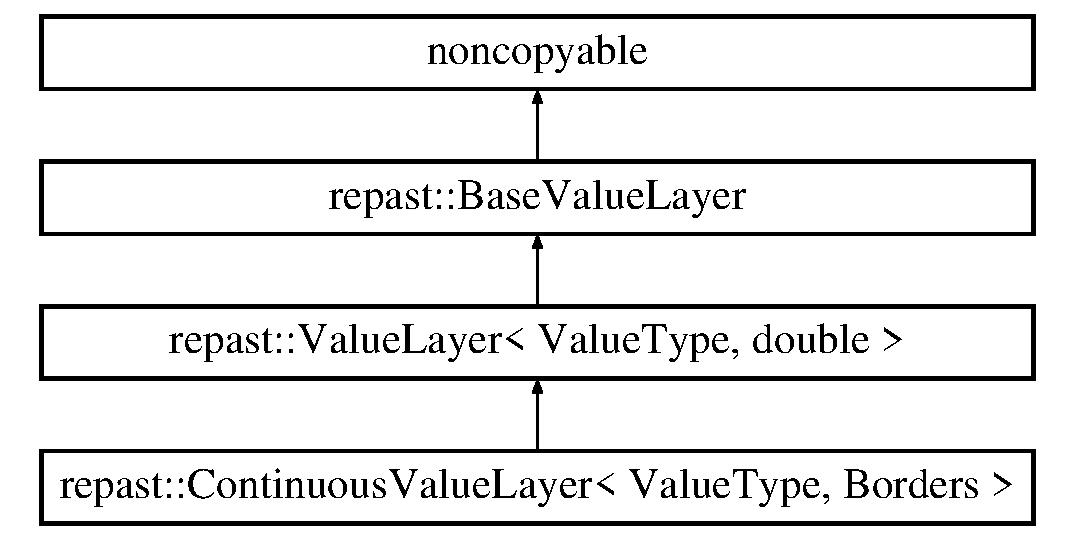
\includegraphics[height=4.000000cm]{classrepast_1_1_continuous_value_layer}
\end{center}
\end{figure}
\subsection*{Public Member Functions}
\begin{DoxyCompactItemize}
\item 
\hypertarget{classrepast_1_1_continuous_value_layer_a89bd9bd46e0bc1b10f1106a88298bdbd}{{\bfseries Continuous\-Value\-Layer} (const \hyperlink{classrepast_1_1_continuous_value_layer}{Continuous\-Value\-Layer}$<$ Value\-Type, \hyperlink{classrepast_1_1_borders}{Borders} $>$ \&other)}\label{classrepast_1_1_continuous_value_layer_a89bd9bd46e0bc1b10f1106a88298bdbd}

\item 
\hypertarget{classrepast_1_1_continuous_value_layer_ae302163efacfefd43908f9ca37574010}{\hyperlink{classrepast_1_1_continuous_value_layer}{Continuous\-Value\-Layer} \& {\bfseries operator=} (const \hyperlink{classrepast_1_1_continuous_value_layer}{Continuous\-Value\-Layer}$<$ Value\-Type, \hyperlink{classrepast_1_1_borders}{Borders} $>$ \&rhs)}\label{classrepast_1_1_continuous_value_layer_ae302163efacfefd43908f9ca37574010}

\item 
\hyperlink{classrepast_1_1_continuous_value_layer_ab5c3df3bdca7ef3b87150f9be3dfc2fe}{Continuous\-Value\-Layer} (const std\-::string \&\hyperlink{classrepast_1_1_base_value_layer_a27277765ee50f9d5446b253f77797f5c}{name}, const \hyperlink{classrepast_1_1_grid_dimensions}{Grid\-Dimensions} \&\hyperlink{classrepast_1_1_value_layer_a51fe7fe718305d0c006bc465a14ef0e3}{dimensions}, const Value\-Type \&default\-Value=Value\-Type())
\begin{DoxyCompactList}\small\item\em Creates a \hyperlink{classrepast_1_1_continuous_value_layer}{Continuous\-Value\-Layer} whose cells contain a default value of Value\-Type() with the specified dimensions. \end{DoxyCompactList}\item 
Value\-Type \& \hyperlink{classrepast_1_1_continuous_value_layer_a020830982b41af4f1d955eee5b617bfa}{get} (const \hyperlink{classrepast_1_1_point}{Point}$<$ double $>$ \&pt)
\begin{DoxyCompactList}\small\item\em Gets the value at the specified point. \end{DoxyCompactList}\item 
void \hyperlink{classrepast_1_1_continuous_value_layer_a619f04cc04200c8de6616ec971674289}{set} (const Value\-Type \&value, const \hyperlink{classrepast_1_1_point}{Point}$<$ double $>$ \&pt)
\begin{DoxyCompactList}\small\item\em Sets the value at the specified point. \end{DoxyCompactList}\end{DoxyCompactItemize}


\subsection{Detailed Description}
\subsubsection*{template$<$typename Value\-Type, typename Borders$>$class repast\-::\-Continuous\-Value\-Layer$<$ Value\-Type, Borders $>$}

Continous value layer whose location coordinates are double. 


\begin{DoxyTemplParams}{Template Parameters}
{\em Value\-Type} & the type of what the value layer stores. \\
\hline
{\em \hyperlink{classrepast_1_1_borders}{Borders}} & the type of borders (wrapped / periodic, strict). Border types can be found in \hyperlink{_grid_components_8h_source}{Grid\-Components.\-h} \\
\hline
\end{DoxyTemplParams}


\subsection{Constructor \& Destructor Documentation}
\hypertarget{classrepast_1_1_continuous_value_layer_ab5c3df3bdca7ef3b87150f9be3dfc2fe}{\index{repast\-::\-Continuous\-Value\-Layer@{repast\-::\-Continuous\-Value\-Layer}!Continuous\-Value\-Layer@{Continuous\-Value\-Layer}}
\index{Continuous\-Value\-Layer@{Continuous\-Value\-Layer}!repast::ContinuousValueLayer@{repast\-::\-Continuous\-Value\-Layer}}
\subsubsection[{Continuous\-Value\-Layer}]{\setlength{\rightskip}{0pt plus 5cm}template$<$typename Value\-Type , typename Borders $>$ {\bf repast\-::\-Continuous\-Value\-Layer}$<$ Value\-Type, {\bf Borders} $>$\-::{\bf Continuous\-Value\-Layer} (
\begin{DoxyParamCaption}
\item[{const std\-::string \&}]{name, }
\item[{const {\bf Grid\-Dimensions} \&}]{dimensions, }
\item[{const Value\-Type \&}]{default\-Value = {\ttfamily ValueType()}}
\end{DoxyParamCaption}
)}}\label{classrepast_1_1_continuous_value_layer_ab5c3df3bdca7ef3b87150f9be3dfc2fe}


Creates a \hyperlink{classrepast_1_1_continuous_value_layer}{Continuous\-Value\-Layer} whose cells contain a default value of Value\-Type() with the specified dimensions. 


\begin{DoxyParams}{Parameters}
{\em name} & the name of the \hyperlink{classrepast_1_1_continuous_value_layer}{Continuous\-Value\-Layer} \\
\hline
{\em dimension} & the dimensions of the \hyperlink{classrepast_1_1_continuous_value_layer}{Continuous\-Value\-Layer} \\
\hline
{\em dense} & whether or not the \hyperlink{classrepast_1_1_value_layer}{Value\-Layer} will be densely populated or not \\
\hline
{\em default\-Value} & the default value to return if no value has been set of a location. The default is the result of Value\-Type(). \\
\hline
\end{DoxyParams}


\subsection{Member Function Documentation}
\hypertarget{classrepast_1_1_continuous_value_layer_a020830982b41af4f1d955eee5b617bfa}{\index{repast\-::\-Continuous\-Value\-Layer@{repast\-::\-Continuous\-Value\-Layer}!get@{get}}
\index{get@{get}!repast::ContinuousValueLayer@{repast\-::\-Continuous\-Value\-Layer}}
\subsubsection[{get}]{\setlength{\rightskip}{0pt plus 5cm}template$<$typename Value\-Type , typename Borders $>$ Value\-Type \& {\bf repast\-::\-Continuous\-Value\-Layer}$<$ Value\-Type, {\bf Borders} $>$\-::get (
\begin{DoxyParamCaption}
\item[{const {\bf Point}$<$ double $>$ \&}]{pt}
\end{DoxyParamCaption}
)\hspace{0.3cm}{\ttfamily [virtual]}}}\label{classrepast_1_1_continuous_value_layer_a020830982b41af4f1d955eee5b617bfa}


Gets the value at the specified point. 

If no value has been set at the specified point then this returns the default value.

param pt the location to get the value of

\begin{DoxyReturn}{Returns}
the value at the specified point, or if no value has been set, then the default value. 
\end{DoxyReturn}


Implements \hyperlink{classrepast_1_1_value_layer_a472a2fcaa29b30c6410ec29b1cde34c0}{repast\-::\-Value\-Layer$<$ Value\-Type, double $>$}.

\hypertarget{classrepast_1_1_continuous_value_layer_a619f04cc04200c8de6616ec971674289}{\index{repast\-::\-Continuous\-Value\-Layer@{repast\-::\-Continuous\-Value\-Layer}!set@{set}}
\index{set@{set}!repast::ContinuousValueLayer@{repast\-::\-Continuous\-Value\-Layer}}
\subsubsection[{set}]{\setlength{\rightskip}{0pt plus 5cm}template$<$typename Value\-Type , typename Borders $>$ void {\bf repast\-::\-Continuous\-Value\-Layer}$<$ Value\-Type, {\bf Borders} $>$\-::set (
\begin{DoxyParamCaption}
\item[{const Value\-Type \&}]{value, }
\item[{const {\bf Point}$<$ double $>$ \&}]{pt}
\end{DoxyParamCaption}
)\hspace{0.3cm}{\ttfamily [virtual]}}}\label{classrepast_1_1_continuous_value_layer_a619f04cc04200c8de6616ec971674289}


Sets the value at the specified point. 


\begin{DoxyParams}{Parameters}
{\em value} & the value \\
\hline
{\em pt} & the point where the value should be stored \\
\hline
\end{DoxyParams}


Implements \hyperlink{classrepast_1_1_value_layer_a34ab3f83380ca978f19748cff9361425}{repast\-::\-Value\-Layer$<$ Value\-Type, double $>$}.



The documentation for this class was generated from the following file\-:\begin{DoxyCompactItemize}
\item 
repast\-\_\-hpc/Value\-Layer.\-h\end{DoxyCompactItemize}

\hypertarget{class_cout_appender}{\section{Cout\-Appender Class Reference}
\label{class_cout_appender}\index{Cout\-Appender@{Cout\-Appender}}
}
Inheritance diagram for Cout\-Appender\-:\begin{figure}[H]
\begin{center}
\leavevmode
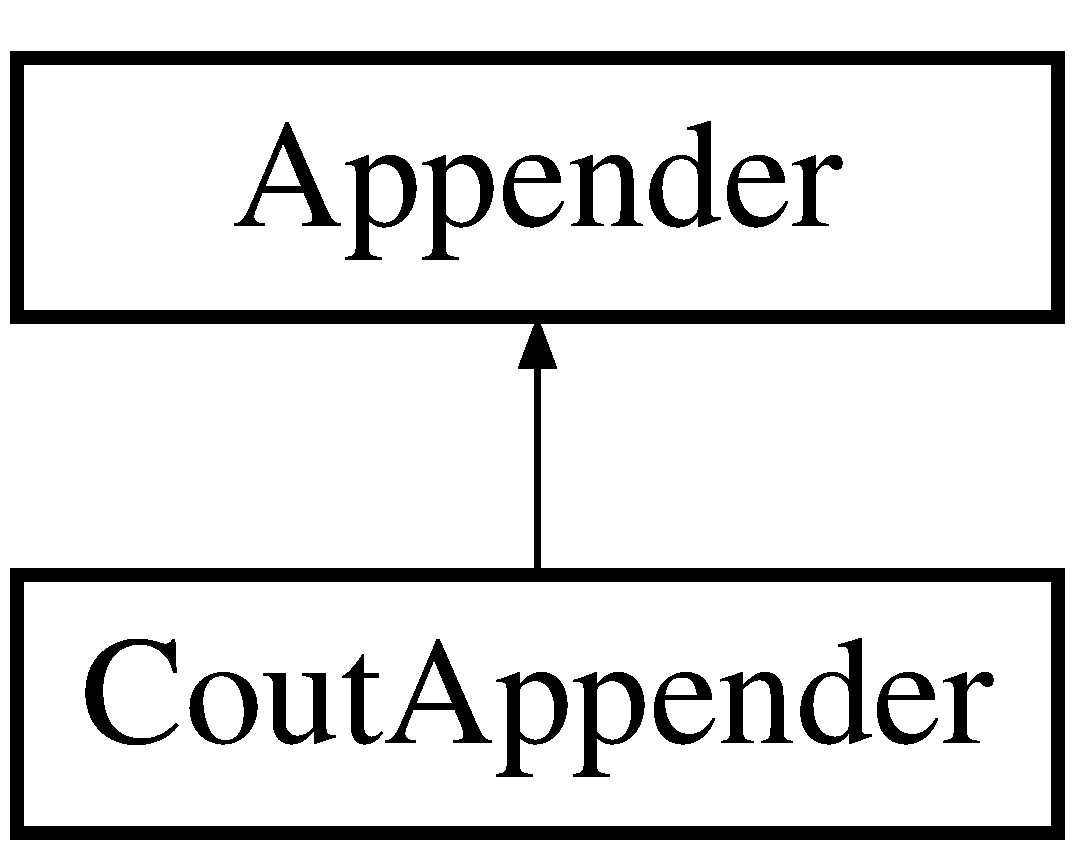
\includegraphics[height=2.000000cm]{class_cout_appender}
\end{center}
\end{figure}
\subsection*{Public Member Functions}
\begin{DoxyCompactItemize}
\item 
\hypertarget{class_cout_appender_a2297ab257bd15bd97c9805123037306b}{void {\bfseries write} (const string \&line)}\label{class_cout_appender_a2297ab257bd15bd97c9805123037306b}

\end{DoxyCompactItemize}
\subsection*{Additional Inherited Members}


The documentation for this class was generated from the following file\-:\begin{DoxyCompactItemize}
\item 
repast\-\_\-hpc/logger.\-cpp\end{DoxyCompactItemize}

\hypertarget{structrepast_1_1data__type__traits}{\section{repast\-:\-:data\-\_\-type\-\_\-traits$<$ T $>$ Struct Template Reference}
\label{structrepast_1_1data__type__traits}\index{repast\-::data\-\_\-type\-\_\-traits$<$ T $>$@{repast\-::data\-\_\-type\-\_\-traits$<$ T $>$}}
}


Base class for specialized int and double type classes.  




{\ttfamily \#include $<$S\-V\-Data\-Source.\-h$>$}



\subsection{Detailed Description}
\subsubsection*{template$<$typename T$>$struct repast\-::data\-\_\-type\-\_\-traits$<$ T $>$}

Base class for specialized int and double type classes. 

The documentation for this struct was generated from the following file\-:\begin{DoxyCompactItemize}
\item 
repast\-\_\-hpc/S\-V\-Data\-Source.\-h\end{DoxyCompactItemize}

\hypertarget{structrepast_1_1data__type__traits_3_01double_01_4}{\section{repast\-:\-:data\-\_\-type\-\_\-traits$<$ double $>$ Struct Template Reference}
\label{structrepast_1_1data__type__traits_3_01double_01_4}\index{repast\-::data\-\_\-type\-\_\-traits$<$ double $>$@{repast\-::data\-\_\-type\-\_\-traits$<$ double $>$}}
}


Double data types for \hyperlink{classrepast_1_1_s_v_data_source}{S\-V\-Data\-Source} objects.  




{\ttfamily \#include $<$S\-V\-Data\-Source.\-h$>$}

\subsection*{Static Public Member Functions}
\begin{DoxyCompactItemize}
\item 
\hypertarget{structrepast_1_1data__type__traits_3_01double_01_4_a396c5e415a3b8b2ce0732860237e3d61}{static S\-V\-Data\-Source\-::\-Data\-Type {\bfseries data\-\_\-type} ()}\label{structrepast_1_1data__type__traits_3_01double_01_4_a396c5e415a3b8b2ce0732860237e3d61}

\end{DoxyCompactItemize}


\subsection{Detailed Description}
\subsubsection*{template$<$$>$struct repast\-::data\-\_\-type\-\_\-traits$<$ double $>$}

Double data types for \hyperlink{classrepast_1_1_s_v_data_source}{S\-V\-Data\-Source} objects. 

The documentation for this struct was generated from the following file\-:\begin{DoxyCompactItemize}
\item 
repast\-\_\-hpc/S\-V\-Data\-Source.\-h\end{DoxyCompactItemize}

\hypertarget{structrepast_1_1data__type__traits_3_01int_01_4}{\section{repast\-:\-:data\-\_\-type\-\_\-traits$<$ int $>$ Struct Template Reference}
\label{structrepast_1_1data__type__traits_3_01int_01_4}\index{repast\-::data\-\_\-type\-\_\-traits$<$ int $>$@{repast\-::data\-\_\-type\-\_\-traits$<$ int $>$}}
}


Int data types for \hyperlink{classrepast_1_1_s_v_data_source}{S\-V\-Data\-Source} objects.  




{\ttfamily \#include $<$S\-V\-Data\-Source.\-h$>$}

\subsection*{Static Public Member Functions}
\begin{DoxyCompactItemize}
\item 
\hypertarget{structrepast_1_1data__type__traits_3_01int_01_4_a0a060997b4e9c8dc6134925c5775a066}{static S\-V\-Data\-Source\-::\-Data\-Type {\bfseries data\-\_\-type} ()}\label{structrepast_1_1data__type__traits_3_01int_01_4_a0a060997b4e9c8dc6134925c5775a066}

\end{DoxyCompactItemize}


\subsection{Detailed Description}
\subsubsection*{template$<$$>$struct repast\-::data\-\_\-type\-\_\-traits$<$ int $>$}

Int data types for \hyperlink{classrepast_1_1_s_v_data_source}{S\-V\-Data\-Source} objects. 

The documentation for this struct was generated from the following file\-:\begin{DoxyCompactItemize}
\item 
repast\-\_\-hpc/S\-V\-Data\-Source.\-h\end{DoxyCompactItemize}

\hypertarget{classrepast_1_1_data_set}{\section{repast\-:\-:Data\-Set Class Reference}
\label{classrepast_1_1_data_set}\index{repast\-::\-Data\-Set@{repast\-::\-Data\-Set}}
}


Interface for recording and writing data.  




{\ttfamily \#include $<$Data\-Set.\-h$>$}

Inheritance diagram for repast\-:\-:Data\-Set\-:\begin{figure}[H]
\begin{center}
\leavevmode
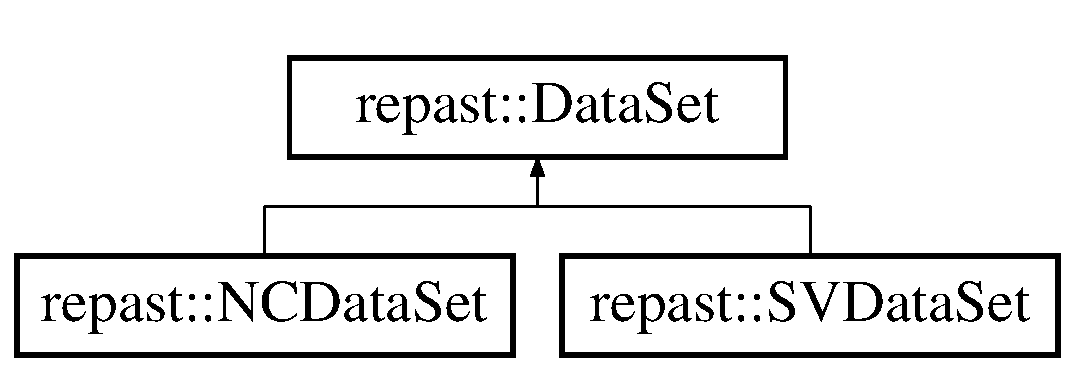
\includegraphics[height=2.000000cm]{classrepast_1_1_data_set}
\end{center}
\end{figure}
\subsection*{Public Member Functions}
\begin{DoxyCompactItemize}
\item 
\hypertarget{classrepast_1_1_data_set_a80bbb8457ca1fae6aa79bed50b64a921}{virtual void \hyperlink{classrepast_1_1_data_set_a80bbb8457ca1fae6aa79bed50b64a921}{record} ()=0}\label{classrepast_1_1_data_set_a80bbb8457ca1fae6aa79bed50b64a921}

\begin{DoxyCompactList}\small\item\em Records the data. \end{DoxyCompactList}\item 
\hypertarget{classrepast_1_1_data_set_a3081affe6d19de1f98a319367c2a3eb6}{virtual void \hyperlink{classrepast_1_1_data_set_a3081affe6d19de1f98a319367c2a3eb6}{write} ()=0}\label{classrepast_1_1_data_set_a3081affe6d19de1f98a319367c2a3eb6}

\begin{DoxyCompactList}\small\item\em Writes the data. \end{DoxyCompactList}\item 
\hypertarget{classrepast_1_1_data_set_a285c971c8a6cfb17c54aa31490b44298}{virtual void \hyperlink{classrepast_1_1_data_set_a285c971c8a6cfb17c54aa31490b44298}{close} ()=0}\label{classrepast_1_1_data_set_a285c971c8a6cfb17c54aa31490b44298}

\begin{DoxyCompactList}\small\item\em Closes the dataset, after which it must be recreated to be used. \end{DoxyCompactList}\end{DoxyCompactItemize}


\subsection{Detailed Description}
Interface for recording and writing data. 

The documentation for this class was generated from the following file\-:\begin{DoxyCompactItemize}
\item 
repast\-\_\-hpc/Data\-Set.\-h\end{DoxyCompactItemize}

\hypertarget{classrepast_1_1_default_number_generator}{\section{repast\-:\-:Default\-Number\-Generator$<$ T $>$ Class Template Reference}
\label{classrepast_1_1_default_number_generator}\index{repast\-::\-Default\-Number\-Generator$<$ T $>$@{repast\-::\-Default\-Number\-Generator$<$ T $>$}}
}


Adapts the templated boost\-::variate\-\_\-generator to the \hyperlink{classrepast_1_1_number_generator}{Number\-Generator} interface.  




{\ttfamily \#include $<$Random.\-h$>$}

Inheritance diagram for repast\-:\-:Default\-Number\-Generator$<$ T $>$\-:\begin{figure}[H]
\begin{center}
\leavevmode
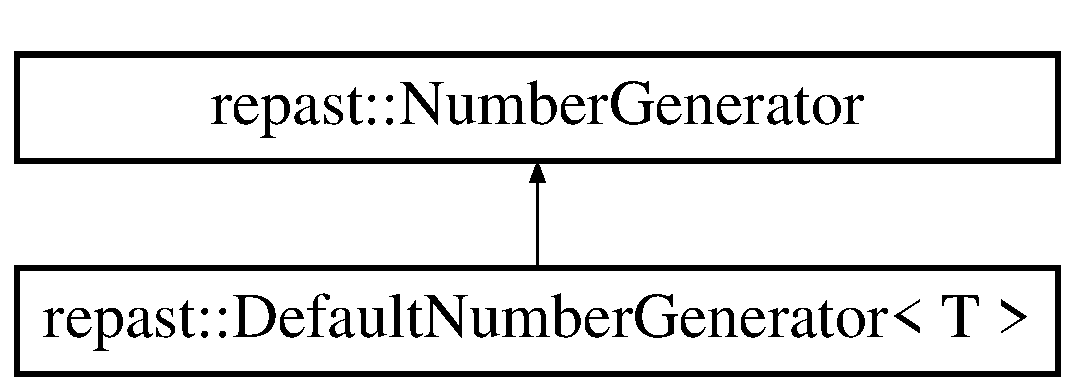
\includegraphics[height=2.000000cm]{classrepast_1_1_default_number_generator}
\end{center}
\end{figure}
\subsection*{Public Member Functions}
\begin{DoxyCompactItemize}
\item 
\hypertarget{classrepast_1_1_default_number_generator_aebb2733213c2385c065b728a57410735}{{\bfseries Default\-Number\-Generator} (T generator)}\label{classrepast_1_1_default_number_generator_aebb2733213c2385c065b728a57410735}

\item 
\hypertarget{classrepast_1_1_default_number_generator_a969fbb9ab8134ba80ff97a6c3a14062f}{double \hyperlink{classrepast_1_1_default_number_generator_a969fbb9ab8134ba80ff97a6c3a14062f}{next} ()}\label{classrepast_1_1_default_number_generator_a969fbb9ab8134ba80ff97a6c3a14062f}

\begin{DoxyCompactList}\small\item\em Gets the \char`\"{}next\char`\"{} number from this Number Generator. \end{DoxyCompactList}\end{DoxyCompactItemize}


\subsection{Detailed Description}
\subsubsection*{template$<$typename T$>$class repast\-::\-Default\-Number\-Generator$<$ T $>$}

Adapts the templated boost\-::variate\-\_\-generator to the \hyperlink{classrepast_1_1_number_generator}{Number\-Generator} interface. 

The documentation for this class was generated from the following file\-:\begin{DoxyCompactItemize}
\item 
repast\-\_\-hpc/Random.\-h\end{DoxyCompactItemize}

\hypertarget{classrepast_1_1_dense_matrix}{\section{repast\-:\-:Dense\-Matrix$<$ T $>$ Class Template Reference}
\label{classrepast_1_1_dense_matrix}\index{repast\-::\-Dense\-Matrix$<$ T $>$@{repast\-::\-Dense\-Matrix$<$ T $>$}}
}


A dense matrix implementation that stores each cell individually.  




{\ttfamily \#include $<$matrix.\-h$>$}

Inheritance diagram for repast\-:\-:Dense\-Matrix$<$ T $>$\-:\begin{figure}[H]
\begin{center}
\leavevmode
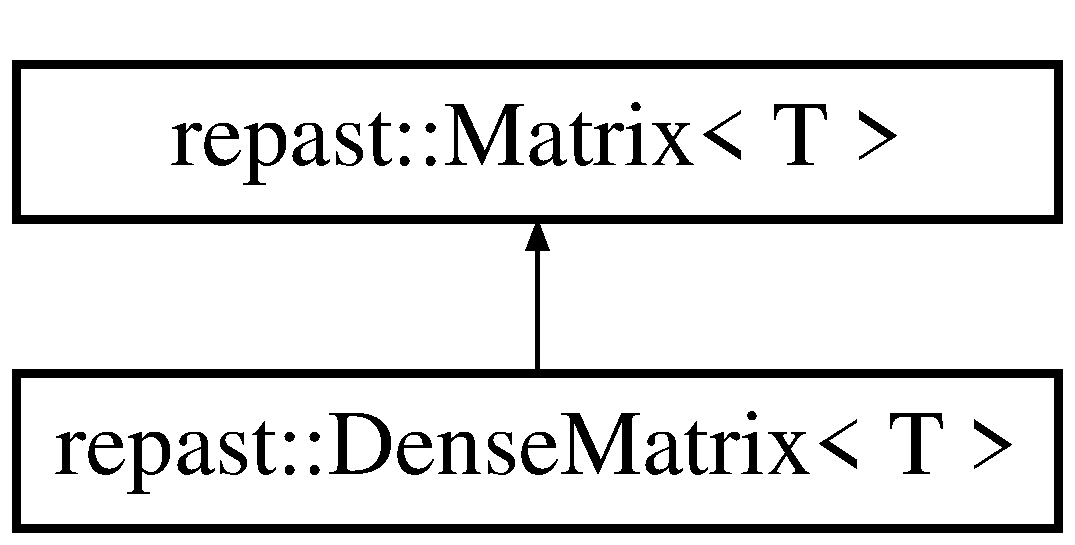
\includegraphics[height=2.000000cm]{classrepast_1_1_dense_matrix}
\end{center}
\end{figure}
\subsection*{Public Member Functions}
\begin{DoxyCompactItemize}
\item 
\hypertarget{classrepast_1_1_dense_matrix_a2d5f88958be7c148ef521187a3a35844}{\hyperlink{classrepast_1_1_dense_matrix_a2d5f88958be7c148ef521187a3a35844}{Dense\-Matrix} (const \hyperlink{classrepast_1_1_dense_matrix}{Dense\-Matrix}$<$ T $>$ \&)}\label{classrepast_1_1_dense_matrix_a2d5f88958be7c148ef521187a3a35844}

\begin{DoxyCompactList}\small\item\em Creates a \hyperlink{classrepast_1_1_dense_matrix}{Dense\-Matrix} as a copy of the specified \hyperlink{classrepast_1_1_dense_matrix}{Dense\-Matrix}. \end{DoxyCompactList}\item 
\hypertarget{classrepast_1_1_dense_matrix_a7f2557ce75a717ac3aa5baa207773d7d}{\hyperlink{classrepast_1_1_dense_matrix}{Dense\-Matrix}$<$ T $>$ \& {\bfseries operator=} (const \hyperlink{classrepast_1_1_dense_matrix}{Dense\-Matrix}$<$ T $>$ \&)}\label{classrepast_1_1_dense_matrix_a7f2557ce75a717ac3aa5baa207773d7d}

\item 
\hypertarget{classrepast_1_1_dense_matrix_a4efadbfd55e04df540cdf11013325ce4}{\hyperlink{classrepast_1_1_dense_matrix_a4efadbfd55e04df540cdf11013325ce4}{Dense\-Matrix} (const \hyperlink{classrepast_1_1_point}{Point}$<$ int $>$ \&\hyperlink{classrepast_1_1_matrix_aa81d61acab94e9de748a647ed3ef535f}{shape}, const T \&def\-Value=T())}\label{classrepast_1_1_dense_matrix_a4efadbfd55e04df540cdf11013325ce4}

\begin{DoxyCompactList}\small\item\em Creates a \hyperlink{classrepast_1_1_dense_matrix}{Dense\-Matrix} of the specified shape and default value. \end{DoxyCompactList}\item 
\hypertarget{classrepast_1_1_dense_matrix_a3f98d3adca4bbf3decefc3cc676a800b}{T \& \hyperlink{classrepast_1_1_dense_matrix_a3f98d3adca4bbf3decefc3cc676a800b}{get} (const \hyperlink{classrepast_1_1_point}{Point}$<$ int $>$ \&index)}\label{classrepast_1_1_dense_matrix_a3f98d3adca4bbf3decefc3cc676a800b}

\begin{DoxyCompactList}\small\item\em Gets the value at the specified index. \end{DoxyCompactList}\item 
\hypertarget{classrepast_1_1_dense_matrix_ab9c2f06db01ab76b2682e376350c16be}{void \hyperlink{classrepast_1_1_dense_matrix_ab9c2f06db01ab76b2682e376350c16be}{set} (const T \&value, const \hyperlink{classrepast_1_1_point}{Point}$<$ int $>$ \&index)}\label{classrepast_1_1_dense_matrix_ab9c2f06db01ab76b2682e376350c16be}

\begin{DoxyCompactList}\small\item\em Sets the value at the specified index. \end{DoxyCompactList}\end{DoxyCompactItemize}
\subsection*{Additional Inherited Members}


\subsection{Detailed Description}
\subsubsection*{template$<$typename T$>$class repast\-::\-Dense\-Matrix$<$ T $>$}

A dense matrix implementation that stores each cell individually. 

The documentation for this class was generated from the following file\-:\begin{DoxyCompactItemize}
\item 
repast\-\_\-hpc/matrix.\-h\end{DoxyCompactItemize}

\hypertarget{classrepast_1_1_directed_vertex}{\section{repast\-:\-:Directed\-Vertex$<$ V, E $>$ Class Template Reference}
\label{classrepast_1_1_directed_vertex}\index{repast\-::\-Directed\-Vertex$<$ V, E $>$@{repast\-::\-Directed\-Vertex$<$ V, E $>$}}
}


Used internally by repast graphs / networks to encapsulate the vertices of a directed graph.  




{\ttfamily \#include $<$Directed\-Vertex.\-h$>$}

Inheritance diagram for repast\-:\-:Directed\-Vertex$<$ V, E $>$\-:\begin{figure}[H]
\begin{center}
\leavevmode
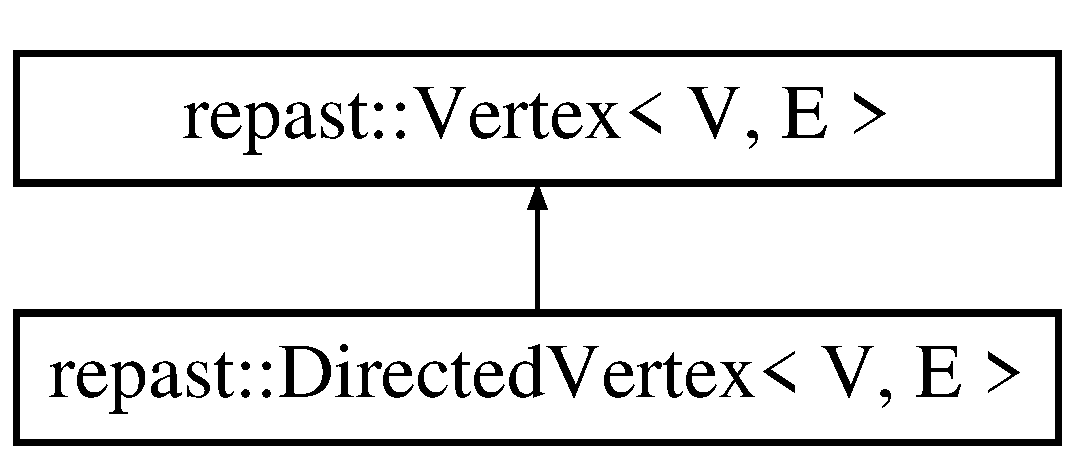
\includegraphics[height=2.000000cm]{classrepast_1_1_directed_vertex}
\end{center}
\end{figure}
\subsection*{Public Member Functions}
\begin{DoxyCompactItemize}
\item 
\hypertarget{classrepast_1_1_directed_vertex_a2f3b536bc1ffa83364808390a19706b7}{\hyperlink{classrepast_1_1_directed_vertex_a2f3b536bc1ffa83364808390a19706b7}{Directed\-Vertex} (boost\-::shared\-\_\-ptr$<$ V $>$ \hyperlink{classrepast_1_1_vertex_a55749dbe0d9f79bb39dfea7733070305}{item})}\label{classrepast_1_1_directed_vertex_a2f3b536bc1ffa83364808390a19706b7}

\begin{DoxyCompactList}\small\item\em Creates a \hyperlink{classrepast_1_1_directed_vertex}{Directed\-Vertex} that will contain the specified item. \end{DoxyCompactList}\item 
virtual boost\-::shared\-\_\-ptr$<$ E $>$ \hyperlink{classrepast_1_1_directed_vertex_ac70277c05d9dbad7bd4d876fd4c4cf5b}{remove\-Edge} (\hyperlink{classrepast_1_1_vertex}{Vertex}$<$ V, E $>$ $\ast$other, \hyperlink{classrepast_1_1_vertex_a8b4819d648c7c0dd8b0622beea77cc14}{Edge\-Type} type)
\begin{DoxyCompactList}\small\item\em Removes the edge of the specified type between this \hyperlink{classrepast_1_1_vertex}{Vertex} and the specified \hyperlink{classrepast_1_1_vertex}{Vertex}. \end{DoxyCompactList}\item 
virtual boost\-::shared\-\_\-ptr$<$ E $>$ \hyperlink{classrepast_1_1_directed_vertex_a1d366144c84a033448fbc0e5f67f8cdb}{find\-Edge} (\hyperlink{classrepast_1_1_vertex}{Vertex}$<$ V, E $>$ $\ast$other, \hyperlink{classrepast_1_1_vertex_a8b4819d648c7c0dd8b0622beea77cc14}{Edge\-Type} type)
\begin{DoxyCompactList}\small\item\em Finds the edge of the specified type between this \hyperlink{classrepast_1_1_vertex}{Vertex} and the specified vertex. \end{DoxyCompactList}\item 
virtual void \hyperlink{classrepast_1_1_directed_vertex_a6ff5f259f8e4087479bb37156b841ab2}{add\-Edge} (\hyperlink{classrepast_1_1_vertex}{Vertex}$<$ V, E $>$ $\ast$other, boost\-::shared\-\_\-ptr$<$ E $>$ edge, \hyperlink{classrepast_1_1_vertex_a8b4819d648c7c0dd8b0622beea77cc14}{Edge\-Type} type)
\begin{DoxyCompactList}\small\item\em Adds an edge of the specified type between this \hyperlink{classrepast_1_1_vertex}{Vertex} and the specified vertex. \end{DoxyCompactList}\item 
virtual void \hyperlink{classrepast_1_1_directed_vertex_a40dc1f60f518eda0ccbf20622ea82839}{successors} (std\-::vector$<$ V $\ast$ $>$ \&out)
\begin{DoxyCompactList}\small\item\em Gets the successors of this \hyperlink{classrepast_1_1_vertex}{Vertex}. \end{DoxyCompactList}\item 
virtual void \hyperlink{classrepast_1_1_directed_vertex_a2b8af860460fa13b4c5e248e266d2ee2}{predecessors} (std\-::vector$<$ V $\ast$ $>$ \&out)
\begin{DoxyCompactList}\small\item\em Gets the predecessors of this \hyperlink{classrepast_1_1_vertex}{Vertex}. \end{DoxyCompactList}\item 
virtual void \hyperlink{classrepast_1_1_directed_vertex_aded5ff0954773ccc6d0e621950e61659}{adjacent} (std\-::vector$<$ V $\ast$ $>$ \&out)
\begin{DoxyCompactList}\small\item\em Gets the Vertices adjacent to this \hyperlink{classrepast_1_1_vertex}{Vertex}. \end{DoxyCompactList}\item 
virtual void \hyperlink{classrepast_1_1_directed_vertex_abdfdf5f45ddd9026017a2ce62e3c5b7e}{edges} (\hyperlink{classrepast_1_1_vertex_a8b4819d648c7c0dd8b0622beea77cc14}{Edge\-Type} type, std\-::vector$<$ boost\-::shared\-\_\-ptr$<$ E $>$ $>$ \&out)
\begin{DoxyCompactList}\small\item\em Gets all the edges of the specified type in which this \hyperlink{classrepast_1_1_vertex}{Vertex} participates and return them in out. \end{DoxyCompactList}\item 
int \hyperlink{classrepast_1_1_directed_vertex_afd409d365742f1b247734c1283cc059a}{in\-Degree} ()
\begin{DoxyCompactList}\small\item\em Gets the in degree of this \hyperlink{classrepast_1_1_vertex}{Vertex}. \end{DoxyCompactList}\item 
int \hyperlink{classrepast_1_1_directed_vertex_a2debe4c699a8cafd8e7bad11f15deca8}{out\-Degree} ()
\begin{DoxyCompactList}\small\item\em Gets the out degree of this \hyperlink{classrepast_1_1_vertex}{Vertex}. \end{DoxyCompactList}\end{DoxyCompactItemize}


\subsection{Detailed Description}
\subsubsection*{template$<$typename V, typename E$>$class repast\-::\-Directed\-Vertex$<$ V, E $>$}

Used internally by repast graphs / networks to encapsulate the vertices of a directed graph. 


\begin{DoxyTemplParams}{Template Parameters}
{\em V} & the type of object stored by in a \hyperlink{classrepast_1_1_vertex}{Vertex}. \\
\hline
{\em E} & the Edge\-Type of the network. \\
\hline
\end{DoxyTemplParams}


\subsection{Member Function Documentation}
\hypertarget{classrepast_1_1_directed_vertex_a6ff5f259f8e4087479bb37156b841ab2}{\index{repast\-::\-Directed\-Vertex@{repast\-::\-Directed\-Vertex}!add\-Edge@{add\-Edge}}
\index{add\-Edge@{add\-Edge}!repast::DirectedVertex@{repast\-::\-Directed\-Vertex}}
\subsubsection[{add\-Edge}]{\setlength{\rightskip}{0pt plus 5cm}template$<$typename V , typename E $>$ void {\bf repast\-::\-Directed\-Vertex}$<$ V, E $>$\-::add\-Edge (
\begin{DoxyParamCaption}
\item[{{\bf Vertex}$<$ V, E $>$ $\ast$}]{other, }
\item[{boost\-::shared\-\_\-ptr$<$ E $>$}]{edge, }
\item[{{\bf Edge\-Type}}]{type}
\end{DoxyParamCaption}
)\hspace{0.3cm}{\ttfamily [virtual]}}}\label{classrepast_1_1_directed_vertex_a6ff5f259f8e4087479bb37156b841ab2}


Adds an edge of the specified type between this \hyperlink{classrepast_1_1_vertex}{Vertex} and the specified vertex. 


\begin{DoxyParams}{Parameters}
{\em edge} & the edge to add \\
\hline
{\em other} & the other end of the edge \\
\hline
{\em type} & the type of edge to add \\
\hline
\end{DoxyParams}


Implements \hyperlink{classrepast_1_1_vertex_a16e732188e59b29be343b96a5377533c}{repast\-::\-Vertex$<$ V, E $>$}.

\hypertarget{classrepast_1_1_directed_vertex_aded5ff0954773ccc6d0e621950e61659}{\index{repast\-::\-Directed\-Vertex@{repast\-::\-Directed\-Vertex}!adjacent@{adjacent}}
\index{adjacent@{adjacent}!repast::DirectedVertex@{repast\-::\-Directed\-Vertex}}
\subsubsection[{adjacent}]{\setlength{\rightskip}{0pt plus 5cm}template$<$typename V , typename E $>$ void {\bf repast\-::\-Directed\-Vertex}$<$ V, E $>$\-::adjacent (
\begin{DoxyParamCaption}
\item[{std\-::vector$<$ V $\ast$ $>$ \&}]{out}
\end{DoxyParamCaption}
)\hspace{0.3cm}{\ttfamily [virtual]}}}\label{classrepast_1_1_directed_vertex_aded5ff0954773ccc6d0e621950e61659}


Gets the Vertices adjacent to this \hyperlink{classrepast_1_1_vertex}{Vertex}. 


\begin{DoxyParams}[1]{Parameters}
\mbox{\tt out}  & {\em the} & vector where the adjacent vectors will be put \\
\hline
\end{DoxyParams}


Implements \hyperlink{classrepast_1_1_vertex_ac0952ef9c988dc4792900ded7d033667}{repast\-::\-Vertex$<$ V, E $>$}.

\hypertarget{classrepast_1_1_directed_vertex_abdfdf5f45ddd9026017a2ce62e3c5b7e}{\index{repast\-::\-Directed\-Vertex@{repast\-::\-Directed\-Vertex}!edges@{edges}}
\index{edges@{edges}!repast::DirectedVertex@{repast\-::\-Directed\-Vertex}}
\subsubsection[{edges}]{\setlength{\rightskip}{0pt plus 5cm}template$<$typename V , typename E $>$ void {\bf repast\-::\-Directed\-Vertex}$<$ V, E $>$\-::edges (
\begin{DoxyParamCaption}
\item[{{\bf Edge\-Type}}]{type, }
\item[{std\-::vector$<$ boost\-::shared\-\_\-ptr$<$ E $>$ $>$ \&}]{out}
\end{DoxyParamCaption}
)\hspace{0.3cm}{\ttfamily [virtual]}}}\label{classrepast_1_1_directed_vertex_abdfdf5f45ddd9026017a2ce62e3c5b7e}


Gets all the edges of the specified type in which this \hyperlink{classrepast_1_1_vertex}{Vertex} participates and return them in out. 


\begin{DoxyParams}[1]{Parameters}
 & {\em type} & the type of edges to get \\
\hline
\mbox{\tt out}  & {\em where} & the edges will be put. \\
\hline
\end{DoxyParams}


Implements \hyperlink{classrepast_1_1_vertex_af652dbbcd2b328685cdd2bb34a7d9240}{repast\-::\-Vertex$<$ V, E $>$}.

\hypertarget{classrepast_1_1_directed_vertex_a1d366144c84a033448fbc0e5f67f8cdb}{\index{repast\-::\-Directed\-Vertex@{repast\-::\-Directed\-Vertex}!find\-Edge@{find\-Edge}}
\index{find\-Edge@{find\-Edge}!repast::DirectedVertex@{repast\-::\-Directed\-Vertex}}
\subsubsection[{find\-Edge}]{\setlength{\rightskip}{0pt plus 5cm}template$<$typename V , typename E $>$ boost\-::shared\-\_\-ptr$<$ E $>$ {\bf repast\-::\-Directed\-Vertex}$<$ V, E $>$\-::find\-Edge (
\begin{DoxyParamCaption}
\item[{{\bf Vertex}$<$ V, E $>$ $\ast$}]{other, }
\item[{{\bf Edge\-Type}}]{type}
\end{DoxyParamCaption}
)\hspace{0.3cm}{\ttfamily [virtual]}}}\label{classrepast_1_1_directed_vertex_a1d366144c84a033448fbc0e5f67f8cdb}


Finds the edge of the specified type between this \hyperlink{classrepast_1_1_vertex}{Vertex} and the specified vertex. 


\begin{DoxyParams}{Parameters}
{\em other} & the other end of the edge \\
\hline
{\em type} & the type of edge to remove\\
\hline
\end{DoxyParams}
\begin{DoxyReturn}{Returns}
the found edge, or 0. 
\end{DoxyReturn}


Implements \hyperlink{classrepast_1_1_vertex_ad649f278be3161b0ee3609019341fe64}{repast\-::\-Vertex$<$ V, E $>$}.

\hypertarget{classrepast_1_1_directed_vertex_afd409d365742f1b247734c1283cc059a}{\index{repast\-::\-Directed\-Vertex@{repast\-::\-Directed\-Vertex}!in\-Degree@{in\-Degree}}
\index{in\-Degree@{in\-Degree}!repast::DirectedVertex@{repast\-::\-Directed\-Vertex}}
\subsubsection[{in\-Degree}]{\setlength{\rightskip}{0pt plus 5cm}template$<$typename V , typename E $>$ int {\bf repast\-::\-Directed\-Vertex}$<$ V, E $>$\-::in\-Degree (
\begin{DoxyParamCaption}
{}
\end{DoxyParamCaption}
)\hspace{0.3cm}{\ttfamily [virtual]}}}\label{classrepast_1_1_directed_vertex_afd409d365742f1b247734c1283cc059a}


Gets the in degree of this \hyperlink{classrepast_1_1_vertex}{Vertex}. 

\begin{DoxyReturn}{Returns}
the in degree of this \hyperlink{classrepast_1_1_vertex}{Vertex}. 
\end{DoxyReturn}


Implements \hyperlink{classrepast_1_1_vertex_a14a787ee4d9ad1069c483b454b8a0004}{repast\-::\-Vertex$<$ V, E $>$}.

\hypertarget{classrepast_1_1_directed_vertex_a2debe4c699a8cafd8e7bad11f15deca8}{\index{repast\-::\-Directed\-Vertex@{repast\-::\-Directed\-Vertex}!out\-Degree@{out\-Degree}}
\index{out\-Degree@{out\-Degree}!repast::DirectedVertex@{repast\-::\-Directed\-Vertex}}
\subsubsection[{out\-Degree}]{\setlength{\rightskip}{0pt plus 5cm}template$<$typename V , typename E $>$ int {\bf repast\-::\-Directed\-Vertex}$<$ V, E $>$\-::out\-Degree (
\begin{DoxyParamCaption}
{}
\end{DoxyParamCaption}
)\hspace{0.3cm}{\ttfamily [virtual]}}}\label{classrepast_1_1_directed_vertex_a2debe4c699a8cafd8e7bad11f15deca8}


Gets the out degree of this \hyperlink{classrepast_1_1_vertex}{Vertex}. 

\begin{DoxyReturn}{Returns}
the out degree of this \hyperlink{classrepast_1_1_vertex}{Vertex}. 
\end{DoxyReturn}


Implements \hyperlink{classrepast_1_1_vertex_a47e058f671914d7c65553bbe20138f33}{repast\-::\-Vertex$<$ V, E $>$}.

\hypertarget{classrepast_1_1_directed_vertex_a2b8af860460fa13b4c5e248e266d2ee2}{\index{repast\-::\-Directed\-Vertex@{repast\-::\-Directed\-Vertex}!predecessors@{predecessors}}
\index{predecessors@{predecessors}!repast::DirectedVertex@{repast\-::\-Directed\-Vertex}}
\subsubsection[{predecessors}]{\setlength{\rightskip}{0pt plus 5cm}template$<$typename V , typename E $>$ void {\bf repast\-::\-Directed\-Vertex}$<$ V, E $>$\-::predecessors (
\begin{DoxyParamCaption}
\item[{std\-::vector$<$ V $\ast$ $>$ \&}]{out}
\end{DoxyParamCaption}
)\hspace{0.3cm}{\ttfamily [virtual]}}}\label{classrepast_1_1_directed_vertex_a2b8af860460fa13b4c5e248e266d2ee2}


Gets the predecessors of this \hyperlink{classrepast_1_1_vertex}{Vertex}. 


\begin{DoxyParams}[1]{Parameters}
\mbox{\tt out}  & {\em the} & vector where any predecessors will be put \\
\hline
\end{DoxyParams}


Implements \hyperlink{classrepast_1_1_vertex_ad27c48d86502b4e73aba445de07c084c}{repast\-::\-Vertex$<$ V, E $>$}.

\hypertarget{classrepast_1_1_directed_vertex_ac70277c05d9dbad7bd4d876fd4c4cf5b}{\index{repast\-::\-Directed\-Vertex@{repast\-::\-Directed\-Vertex}!remove\-Edge@{remove\-Edge}}
\index{remove\-Edge@{remove\-Edge}!repast::DirectedVertex@{repast\-::\-Directed\-Vertex}}
\subsubsection[{remove\-Edge}]{\setlength{\rightskip}{0pt plus 5cm}template$<$typename V , typename E $>$ boost\-::shared\-\_\-ptr$<$ E $>$ {\bf repast\-::\-Directed\-Vertex}$<$ V, E $>$\-::remove\-Edge (
\begin{DoxyParamCaption}
\item[{{\bf Vertex}$<$ V, E $>$ $\ast$}]{other, }
\item[{{\bf Edge\-Type}}]{type}
\end{DoxyParamCaption}
)\hspace{0.3cm}{\ttfamily [virtual]}}}\label{classrepast_1_1_directed_vertex_ac70277c05d9dbad7bd4d876fd4c4cf5b}


Removes the edge of the specified type between this \hyperlink{classrepast_1_1_vertex}{Vertex} and the specified \hyperlink{classrepast_1_1_vertex}{Vertex}. 


\begin{DoxyParams}{Parameters}
{\em other} & the other end of the edge \\
\hline
{\em type} & the type of edge to remove\\
\hline
\end{DoxyParams}
\begin{DoxyReturn}{Returns}
the removed edge if such an edge was found, otherwise 0. 
\end{DoxyReturn}


Implements \hyperlink{classrepast_1_1_vertex_ac3ac362e00073965fc501b2671e908eb}{repast\-::\-Vertex$<$ V, E $>$}.

\hypertarget{classrepast_1_1_directed_vertex_a40dc1f60f518eda0ccbf20622ea82839}{\index{repast\-::\-Directed\-Vertex@{repast\-::\-Directed\-Vertex}!successors@{successors}}
\index{successors@{successors}!repast::DirectedVertex@{repast\-::\-Directed\-Vertex}}
\subsubsection[{successors}]{\setlength{\rightskip}{0pt plus 5cm}template$<$typename V , typename E $>$ void {\bf repast\-::\-Directed\-Vertex}$<$ V, E $>$\-::successors (
\begin{DoxyParamCaption}
\item[{std\-::vector$<$ V $\ast$ $>$ \&}]{out}
\end{DoxyParamCaption}
)\hspace{0.3cm}{\ttfamily [virtual]}}}\label{classrepast_1_1_directed_vertex_a40dc1f60f518eda0ccbf20622ea82839}


Gets the successors of this \hyperlink{classrepast_1_1_vertex}{Vertex}. 


\begin{DoxyParams}[1]{Parameters}
\mbox{\tt out}  & {\em the} & vector where any successors will be put \\
\hline
\end{DoxyParams}


Implements \hyperlink{classrepast_1_1_vertex_a0e3a2812db0b42ca344bd577076002d0}{repast\-::\-Vertex$<$ V, E $>$}.



The documentation for this class was generated from the following file\-:\begin{DoxyCompactItemize}
\item 
repast\-\_\-hpc/Directed\-Vertex.\-h\end{DoxyCompactItemize}

\hypertarget{classrepast_1_1_discrete_value_layer}{\section{repast\-:\-:Discrete\-Value\-Layer$<$ Value\-Type, Borders $>$ Class Template Reference}
\label{classrepast_1_1_discrete_value_layer}\index{repast\-::\-Discrete\-Value\-Layer$<$ Value\-Type, Borders $>$@{repast\-::\-Discrete\-Value\-Layer$<$ Value\-Type, Borders $>$}}
}


Creates \hyperlink{classrepast_1_1_value_layer}{Value\-Layer} whose location coordinates are ints.  




{\ttfamily \#include $<$Value\-Layer.\-h$>$}

Inheritance diagram for repast\-:\-:Discrete\-Value\-Layer$<$ Value\-Type, Borders $>$\-:\begin{figure}[H]
\begin{center}
\leavevmode
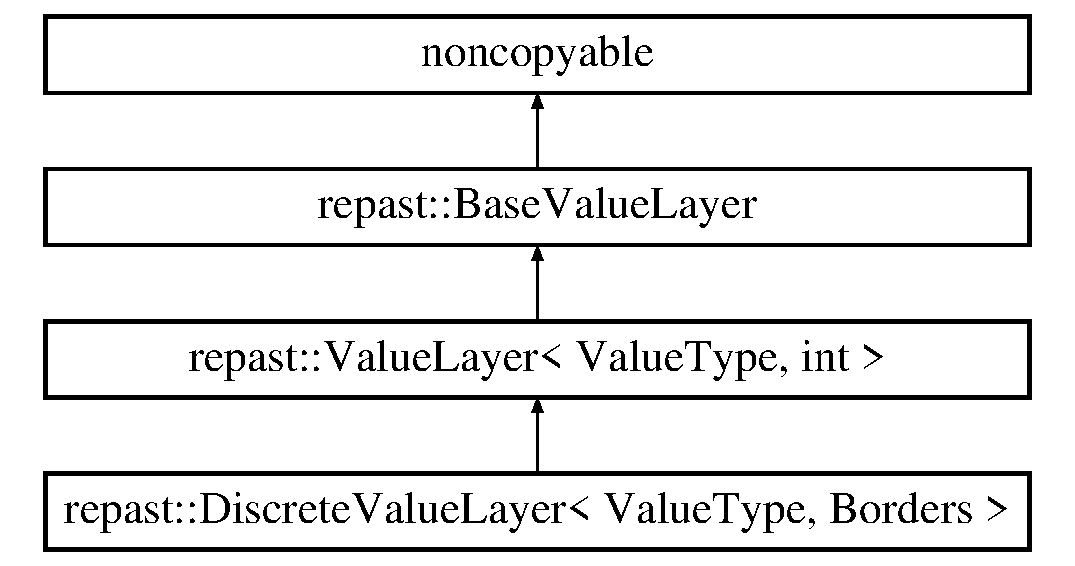
\includegraphics[height=4.000000cm]{classrepast_1_1_discrete_value_layer}
\end{center}
\end{figure}
\subsection*{Public Member Functions}
\begin{DoxyCompactItemize}
\item 
\hypertarget{classrepast_1_1_discrete_value_layer_aae74c061422347ebccf0163db1f0998f}{{\bfseries Discrete\-Value\-Layer} (const \hyperlink{classrepast_1_1_discrete_value_layer}{Discrete\-Value\-Layer}$<$ Value\-Type, \hyperlink{classrepast_1_1_borders}{Borders} $>$ \&other)}\label{classrepast_1_1_discrete_value_layer_aae74c061422347ebccf0163db1f0998f}

\item 
\hypertarget{classrepast_1_1_discrete_value_layer_aaea82e29c4e38e63e7921b1d83895654}{\hyperlink{classrepast_1_1_discrete_value_layer}{Discrete\-Value\-Layer} \& {\bfseries operator=} (const \hyperlink{classrepast_1_1_discrete_value_layer}{Discrete\-Value\-Layer}$<$ Value\-Type, \hyperlink{classrepast_1_1_borders}{Borders} $>$ \&rhs)}\label{classrepast_1_1_discrete_value_layer_aaea82e29c4e38e63e7921b1d83895654}

\item 
\hyperlink{classrepast_1_1_discrete_value_layer_a146b16f54f9b13ccfeb6462f359d0203}{Discrete\-Value\-Layer} (const std\-::string \&\hyperlink{classrepast_1_1_base_value_layer_a27277765ee50f9d5446b253f77797f5c}{name}, const \hyperlink{classrepast_1_1_grid_dimensions}{Grid\-Dimensions} \&\hyperlink{classrepast_1_1_value_layer_a51fe7fe718305d0c006bc465a14ef0e3}{dimensions}, bool dense, const Value\-Type \&default\-Value=Value\-Type())
\begin{DoxyCompactList}\small\item\em Creates a \hyperlink{classrepast_1_1_discrete_value_layer}{Discrete\-Value\-Layer} whose cells contain a default value of Value\-Type() with the specified dimensions. \end{DoxyCompactList}\item 
Value\-Type \& \hyperlink{classrepast_1_1_discrete_value_layer_abf7996a02382f6a28b3d993a156386c7}{get} (const \hyperlink{classrepast_1_1_point}{Point}$<$ int $>$ \&pt)
\begin{DoxyCompactList}\small\item\em Gets the value at the specified point. \end{DoxyCompactList}\item 
void \hyperlink{classrepast_1_1_discrete_value_layer_a2070dcc808c4d5b48de96b278f8a8d89}{set} (const Value\-Type \&value, const \hyperlink{classrepast_1_1_point}{Point}$<$ int $>$ \&pt)
\begin{DoxyCompactList}\small\item\em Sets the value at the specified point. \end{DoxyCompactList}\end{DoxyCompactItemize}


\subsection{Detailed Description}
\subsubsection*{template$<$typename Value\-Type, typename Borders$>$class repast\-::\-Discrete\-Value\-Layer$<$ Value\-Type, Borders $>$}

Creates \hyperlink{classrepast_1_1_value_layer}{Value\-Layer} whose location coordinates are ints. 


\begin{DoxyTemplParams}{Template Parameters}
{\em Value\-Type} & the type of what the value layer stores. \\
\hline
{\em \hyperlink{classrepast_1_1_borders}{Borders}} & the type of borders (wrapped / periodic, strict). Border types can be found in \hyperlink{_grid_components_8h_source}{Grid\-Components.\-h} \\
\hline
\end{DoxyTemplParams}


\subsection{Constructor \& Destructor Documentation}
\hypertarget{classrepast_1_1_discrete_value_layer_a146b16f54f9b13ccfeb6462f359d0203}{\index{repast\-::\-Discrete\-Value\-Layer@{repast\-::\-Discrete\-Value\-Layer}!Discrete\-Value\-Layer@{Discrete\-Value\-Layer}}
\index{Discrete\-Value\-Layer@{Discrete\-Value\-Layer}!repast::DiscreteValueLayer@{repast\-::\-Discrete\-Value\-Layer}}
\subsubsection[{Discrete\-Value\-Layer}]{\setlength{\rightskip}{0pt plus 5cm}template$<$typename Value\-Type , typename Borders $>$ {\bf repast\-::\-Discrete\-Value\-Layer}$<$ Value\-Type, {\bf Borders} $>$\-::{\bf Discrete\-Value\-Layer} (
\begin{DoxyParamCaption}
\item[{const std\-::string \&}]{name, }
\item[{const {\bf Grid\-Dimensions} \&}]{dimensions, }
\item[{bool}]{dense, }
\item[{const Value\-Type \&}]{default\-Value = {\ttfamily ValueType()}}
\end{DoxyParamCaption}
)}}\label{classrepast_1_1_discrete_value_layer_a146b16f54f9b13ccfeb6462f359d0203}


Creates a \hyperlink{classrepast_1_1_discrete_value_layer}{Discrete\-Value\-Layer} whose cells contain a default value of Value\-Type() with the specified dimensions. 


\begin{DoxyParams}{Parameters}
{\em name} & the name of the \hyperlink{classrepast_1_1_discrete_value_layer}{Discrete\-Value\-Layer} \\
\hline
{\em dimension} & the dimensions of the \hyperlink{classrepast_1_1_discrete_value_layer}{Discrete\-Value\-Layer} \\
\hline
{\em dense} & whether or not the \hyperlink{classrepast_1_1_value_layer}{Value\-Layer} will be densely populated or not \\
\hline
{\em default\-Value} & the default value to return if no value has been set of a location. The default is the result of Value\-Type(). \\
\hline
\end{DoxyParams}


\subsection{Member Function Documentation}
\hypertarget{classrepast_1_1_discrete_value_layer_abf7996a02382f6a28b3d993a156386c7}{\index{repast\-::\-Discrete\-Value\-Layer@{repast\-::\-Discrete\-Value\-Layer}!get@{get}}
\index{get@{get}!repast::DiscreteValueLayer@{repast\-::\-Discrete\-Value\-Layer}}
\subsubsection[{get}]{\setlength{\rightskip}{0pt plus 5cm}template$<$typename Value\-Type , typename Borders $>$ Value\-Type \& {\bf repast\-::\-Discrete\-Value\-Layer}$<$ Value\-Type, {\bf Borders} $>$\-::get (
\begin{DoxyParamCaption}
\item[{const {\bf Point}$<$ int $>$ \&}]{pt}
\end{DoxyParamCaption}
)\hspace{0.3cm}{\ttfamily [virtual]}}}\label{classrepast_1_1_discrete_value_layer_abf7996a02382f6a28b3d993a156386c7}


Gets the value at the specified point. 

If no value has been set at the specified point then this returns the default value.

param pt the location to get the value of

\begin{DoxyReturn}{Returns}
the value at the specified point, or if no value has been set, then the default value. 
\end{DoxyReturn}


Implements \hyperlink{classrepast_1_1_value_layer_a472a2fcaa29b30c6410ec29b1cde34c0}{repast\-::\-Value\-Layer$<$ Value\-Type, int $>$}.

\hypertarget{classrepast_1_1_discrete_value_layer_a2070dcc808c4d5b48de96b278f8a8d89}{\index{repast\-::\-Discrete\-Value\-Layer@{repast\-::\-Discrete\-Value\-Layer}!set@{set}}
\index{set@{set}!repast::DiscreteValueLayer@{repast\-::\-Discrete\-Value\-Layer}}
\subsubsection[{set}]{\setlength{\rightskip}{0pt plus 5cm}template$<$typename Value\-Type , typename Borders $>$ void {\bf repast\-::\-Discrete\-Value\-Layer}$<$ Value\-Type, {\bf Borders} $>$\-::set (
\begin{DoxyParamCaption}
\item[{const Value\-Type \&}]{value, }
\item[{const {\bf Point}$<$ int $>$ \&}]{pt}
\end{DoxyParamCaption}
)\hspace{0.3cm}{\ttfamily [virtual]}}}\label{classrepast_1_1_discrete_value_layer_a2070dcc808c4d5b48de96b278f8a8d89}


Sets the value at the specified point. 


\begin{DoxyParams}{Parameters}
{\em value} & the value \\
\hline
{\em pt} & the point where the value should be stored \\
\hline
\end{DoxyParams}


Implements \hyperlink{classrepast_1_1_value_layer_a34ab3f83380ca978f19748cff9361425}{repast\-::\-Value\-Layer$<$ Value\-Type, int $>$}.



The documentation for this class was generated from the following file\-:\begin{DoxyCompactItemize}
\item 
repast\-\_\-hpc/Value\-Layer.\-h\end{DoxyCompactItemize}

\hypertarget{classrepast_1_1_double_variable}{\section{repast\-:\-:Double\-Variable Class Reference}
\label{classrepast_1_1_double_variable}\index{repast\-::\-Double\-Variable@{repast\-::\-Double\-Variable}}
}


Used in \hyperlink{classrepast_1_1_s_v_data_set}{S\-V\-Data\-Set} to manage double data.  




{\ttfamily \#include $<$Variable.\-h$>$}

Inheritance diagram for repast\-:\-:Double\-Variable\-:\begin{figure}[H]
\begin{center}
\leavevmode
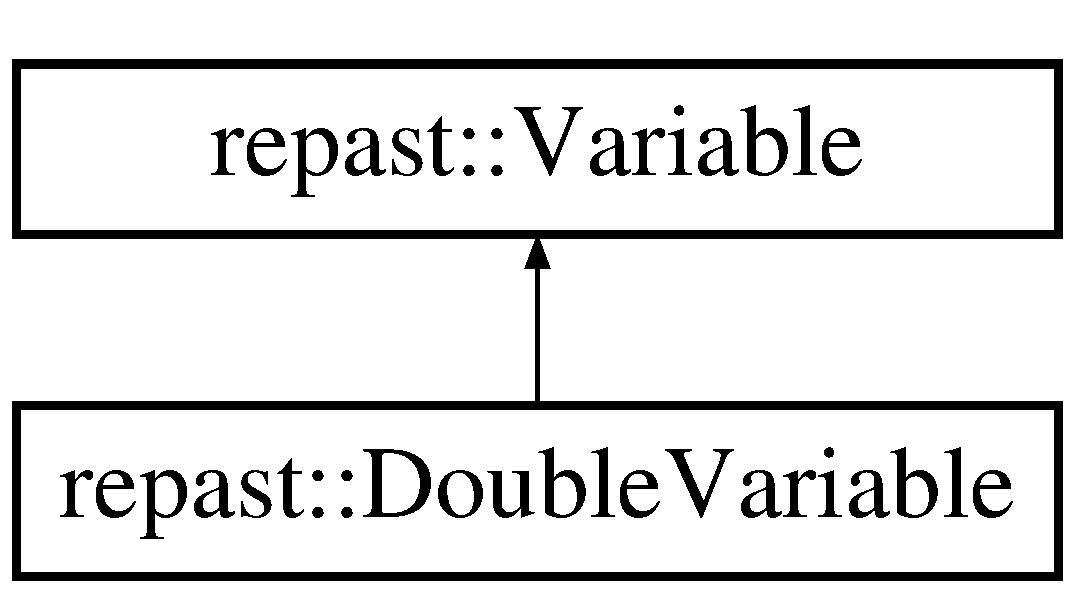
\includegraphics[height=2.000000cm]{classrepast_1_1_double_variable}
\end{center}
\end{figure}
\subsection*{Public Member Functions}
\begin{DoxyCompactItemize}
\item 
virtual void \hyperlink{classrepast_1_1_double_variable_ae6edc7abb29517ba7b8b77f776a7c223}{write} (size\-\_\-t index, std\-::ofstream \&out)
\begin{DoxyCompactList}\small\item\em Writes the data at the specified index to the specified ofstream. \end{DoxyCompactList}\item 
virtual void \hyperlink{classrepast_1_1_double_variable_a9b7e645d7b1c772b7fd8928a3aca6e65}{insert} (double $\ast$array, size\-\_\-t size)
\begin{DoxyCompactList}\small\item\em Inserts all the doubles in the double array into the collection of data stored in this \hyperlink{classrepast_1_1_variable}{Variable}. \end{DoxyCompactList}\item 
virtual void \hyperlink{classrepast_1_1_double_variable_a234cac0e0fbfd60d724fcae3a8edcc63}{insert} (int $\ast$array, size\-\_\-t size)
\begin{DoxyCompactList}\small\item\em Inserts all the ints in the int array into the collection of data stored in this \hyperlink{classrepast_1_1_variable}{Variable}. \end{DoxyCompactList}\item 
\hypertarget{classrepast_1_1_double_variable_ad9952aa7bc0691d19757b10013e36e0e}{virtual void \hyperlink{classrepast_1_1_double_variable_ad9952aa7bc0691d19757b10013e36e0e}{clear} ()}\label{classrepast_1_1_double_variable_ad9952aa7bc0691d19757b10013e36e0e}

\begin{DoxyCompactList}\small\item\em Clears this \hyperlink{classrepast_1_1_variable}{Variable} of all the data stored in it. \end{DoxyCompactList}\end{DoxyCompactItemize}


\subsection{Detailed Description}
Used in \hyperlink{classrepast_1_1_s_v_data_set}{S\-V\-Data\-Set} to manage double data. 

\subsection{Member Function Documentation}
\hypertarget{classrepast_1_1_double_variable_a9b7e645d7b1c772b7fd8928a3aca6e65}{\index{repast\-::\-Double\-Variable@{repast\-::\-Double\-Variable}!insert@{insert}}
\index{insert@{insert}!repast::DoubleVariable@{repast\-::\-Double\-Variable}}
\subsubsection[{insert}]{\setlength{\rightskip}{0pt plus 5cm}void repast\-::\-Double\-Variable\-::insert (
\begin{DoxyParamCaption}
\item[{double $\ast$}]{array, }
\item[{size\-\_\-t}]{size}
\end{DoxyParamCaption}
)\hspace{0.3cm}{\ttfamily [virtual]}}}\label{classrepast_1_1_double_variable_a9b7e645d7b1c772b7fd8928a3aca6e65}


Inserts all the doubles in the double array into the collection of data stored in this \hyperlink{classrepast_1_1_variable}{Variable}. 


\begin{DoxyParams}{Parameters}
{\em array} & the array to insert \\
\hline
{\em size} & the size of the array \\
\hline
\end{DoxyParams}


Implements \hyperlink{classrepast_1_1_variable_ac87aada07f0b7ee34d6fbd2486016eb8}{repast\-::\-Variable}.

\hypertarget{classrepast_1_1_double_variable_a234cac0e0fbfd60d724fcae3a8edcc63}{\index{repast\-::\-Double\-Variable@{repast\-::\-Double\-Variable}!insert@{insert}}
\index{insert@{insert}!repast::DoubleVariable@{repast\-::\-Double\-Variable}}
\subsubsection[{insert}]{\setlength{\rightskip}{0pt plus 5cm}void repast\-::\-Double\-Variable\-::insert (
\begin{DoxyParamCaption}
\item[{int $\ast$}]{array, }
\item[{size\-\_\-t}]{size}
\end{DoxyParamCaption}
)\hspace{0.3cm}{\ttfamily [virtual]}}}\label{classrepast_1_1_double_variable_a234cac0e0fbfd60d724fcae3a8edcc63}


Inserts all the ints in the int array into the collection of data stored in this \hyperlink{classrepast_1_1_variable}{Variable}. 


\begin{DoxyParams}{Parameters}
{\em array} & the array to insert \\
\hline
{\em size} & the size of the array \\
\hline
\end{DoxyParams}


Implements \hyperlink{classrepast_1_1_variable_a5f625f2652dcbc9c1910539923475936}{repast\-::\-Variable}.

\hypertarget{classrepast_1_1_double_variable_ae6edc7abb29517ba7b8b77f776a7c223}{\index{repast\-::\-Double\-Variable@{repast\-::\-Double\-Variable}!write@{write}}
\index{write@{write}!repast::DoubleVariable@{repast\-::\-Double\-Variable}}
\subsubsection[{write}]{\setlength{\rightskip}{0pt plus 5cm}void repast\-::\-Double\-Variable\-::write (
\begin{DoxyParamCaption}
\item[{size\-\_\-t}]{index, }
\item[{std\-::ofstream \&}]{out}
\end{DoxyParamCaption}
)\hspace{0.3cm}{\ttfamily [virtual]}}}\label{classrepast_1_1_double_variable_ae6edc7abb29517ba7b8b77f776a7c223}


Writes the data at the specified index to the specified ofstream. 


\begin{DoxyParams}{Parameters}
{\em index} & the index of the data to write \\
\hline
{\em out} & the ofstream to write the data to \\
\hline
\end{DoxyParams}


Implements \hyperlink{classrepast_1_1_variable_aa72da48bdca530dd7878b912254568e0}{repast\-::\-Variable}.



The documentation for this class was generated from the following files\-:\begin{DoxyCompactItemize}
\item 
repast\-\_\-hpc/Variable.\-h\item 
repast\-\_\-hpc/Variable.\-cpp\end{DoxyCompactItemize}

\hypertarget{classrepast_1_1_edge_exporter}{\section{repast\-:\-:Edge\-Exporter$<$ E $>$ Class Template Reference}
\label{classrepast_1_1_edge_exporter}\index{repast\-::\-Edge\-Exporter$<$ E $>$@{repast\-::\-Edge\-Exporter$<$ E $>$}}
}


{\itshape D\-E\-P\-R\-E\-C\-A\-T\-E\-D} Handles exporting edges created locally between one or more non-\/local agents.  




{\ttfamily \#include $<$Shared\-Network.\-h$>$}

\subsection*{Public Types}
\begin{DoxyCompactItemize}
\item 
\hypertarget{classrepast_1_1_edge_exporter_a035179ca3839797ba3b3dec950e5f029}{typedef std\-::map$<$ int, \\*
std\-::vector$<$ boost\-::shared\-\_\-ptr\\*
$<$ E $>$ $>$ $\ast$ $>$\-::iterator {\bfseries Edge\-Map\-Iterator}}\label{classrepast_1_1_edge_exporter_a035179ca3839797ba3b3dec950e5f029}

\end{DoxyCompactItemize}
\subsection*{Public Member Functions}
\begin{DoxyCompactItemize}
\item 
\hypertarget{classrepast_1_1_edge_exporter_ae987c31a445fcbee65ec409ae6f4306c}{void {\bfseries add\-Agent\-Export\-Request} (int export\-To, const \hyperlink{classrepast_1_1_agent_id}{Agent\-Id} \&id)}\label{classrepast_1_1_edge_exporter_ae987c31a445fcbee65ec409ae6f4306c}

\item 
\hypertarget{classrepast_1_1_edge_exporter_a4d60a45bb6ea9de3ba989f7708fdedb8}{void \hyperlink{classrepast_1_1_edge_exporter_a4d60a45bb6ea9de3ba989f7708fdedb8}{edge\-Removed} (boost\-::shared\-\_\-ptr$<$ E $>$ edge, std\-::map$<$ int, std\-::vector$<$ std\-::pair$<$ \hyperlink{classrepast_1_1_agent_id}{Agent\-Id}, \hyperlink{classrepast_1_1_agent_id}{Agent\-Id} $>$ $>$ $>$ \&remove\-Map)}\label{classrepast_1_1_edge_exporter_a4d60a45bb6ea9de3ba989f7708fdedb8}

\begin{DoxyCompactList}\small\item\em Whether or not this is exported the specified edge. \end{DoxyCompactList}\item 
\hypertarget{classrepast_1_1_edge_exporter_a1799f762f412c81d2c60cc0337474e09}{void \hyperlink{classrepast_1_1_edge_exporter_a1799f762f412c81d2c60cc0337474e09}{add\-Edge} (boost\-::shared\-\_\-ptr$<$ E $>$ edge)}\label{classrepast_1_1_edge_exporter_a1799f762f412c81d2c60cc0337474e09}

\begin{DoxyCompactList}\small\item\em Tests if the edge needs to be exported and if so adds it to the collection of edges to be exported. \end{DoxyCompactList}\item 
void \hyperlink{classrepast_1_1_edge_exporter_ab748591b5dccdda31042a8ba989fd1a2}{gather\-Receivers} (std\-::vector$<$ int $>$ \&out)
\begin{DoxyCompactList}\small\item\em Gathers the receivers into out. \end{DoxyCompactList}\item 
\hypertarget{classrepast_1_1_edge_exporter_a14848eca966380f353a30792bc79fab9}{void \hyperlink{classrepast_1_1_edge_exporter_a14848eca966380f353a30792bc79fab9}{gather\-Exporters} (std\-::vector$<$ int $>$ \&out)}\label{classrepast_1_1_edge_exporter_a14848eca966380f353a30792bc79fab9}

\begin{DoxyCompactList}\small\item\em Gathers the procs that this will send export requests to into out. \end{DoxyCompactList}\item 
void \hyperlink{classrepast_1_1_edge_exporter_a8c4c03a3c019fddfbdd50a0f18720da0}{send\-Export\-Requests} (boost\-::mpi\-::communicator \&comm, std\-::vector$<$ boost\-::mpi\-::request $>$ \&requests)
\begin{DoxyCompactList}\small\item\em Send the export requests. \end{DoxyCompactList}\item 
\hypertarget{classrepast_1_1_edge_exporter_af90d243e08c23ac3c54d285e43cf3610}{std\-::map$<$ int, std\-::vector\\*
$<$ boost\-::shared\-\_\-ptr$<$ E $>$ $>$ $\ast$ $>$ \& \hyperlink{classrepast_1_1_edge_exporter_af90d243e08c23ac3c54d285e43cf3610}{get\-Edges\-To\-Export} ()}\label{classrepast_1_1_edge_exporter_af90d243e08c23ac3c54d285e43cf3610}

\begin{DoxyCompactList}\small\item\em Gets the edges to export. \end{DoxyCompactList}\item 
\hypertarget{classrepast_1_1_edge_exporter_af5938ec2539d124780a95064b109a96b}{std\-::map$<$ int, std\-::vector\\*
$<$ boost\-::shared\-\_\-ptr$<$ E $>$ $>$ $\ast$ $>$ \& \hyperlink{classrepast_1_1_edge_exporter_af5938ec2539d124780a95064b109a96b}{get\-Exported\-Edges} ()}\label{classrepast_1_1_edge_exporter_af5938ec2539d124780a95064b109a96b}

\begin{DoxyCompactList}\small\item\em Gets the edges this process is exporting. \end{DoxyCompactList}\item 
\hypertarget{classrepast_1_1_edge_exporter_a3ced9c3a093fe4666f9c82d4bd2c6d83}{void \hyperlink{classrepast_1_1_edge_exporter_a3ced9c3a093fe4666f9c82d4bd2c6d83}{clean\-Up} ()}\label{classrepast_1_1_edge_exporter_a3ced9c3a093fe4666f9c82d4bd2c6d83}

\begin{DoxyCompactList}\small\item\em Cleans up after exported edges have been sent and received. \end{DoxyCompactList}\end{DoxyCompactItemize}
\subsection*{Friends}
\begin{DoxyCompactItemize}
\item 
{\footnotesize template$<$typename Vertex , typename Edge , typename Agent\-Content , typename Edge\-Content , typename Edge\-Manager , typename Agent\-Creator $>$ }\\void \hyperlink{classrepast_1_1_edge_exporter_aab38d29bc953ebb66d39ecb27f392acf}{create\-Complementary\-Edges} (\hyperlink{classrepast_1_1_shared_network}{Shared\-Network}$<$ \hyperlink{classrepast_1_1_vertex}{Vertex}, Edge, Edge\-Content, Edge\-Manager $>$ $\ast$net, \hyperlink{classrepast_1_1_shared_context}{Shared\-Context}$<$ \hyperlink{classrepast_1_1_vertex}{Vertex} $>$ \&context, Edge\-Manager \&edge\-Manager, Agent\-Creator \&creator)
\begin{DoxyCompactList}\small\item\em Notifies other processes of any edges that have been created between nodes on this process and imported nodes. \end{DoxyCompactList}\end{DoxyCompactItemize}


\subsection{Detailed Description}
\subsubsection*{template$<$typename E$>$class repast\-::\-Edge\-Exporter$<$ E $>$}

{\itshape D\-E\-P\-R\-E\-C\-A\-T\-E\-D} Handles exporting edges created locally between one or more non-\/local agents. 

This also coordinates notification of which processes should be exporting to which in the case of edges where a node is foreign to the sending and receiving process.

All this is done internally in the \hyperlink{classrepast_1_1_shared_network}{Shared\-Network}.

\begin{DoxyRefDesc}{Deprecated}
\item[\hyperlink{deprecated__deprecated000005}{Deprecated}]As of Version 2.\-0 replaced by \hyperlink{classrepast_1_1_projection_info_packet}{Projection\-Info\-Packet} \end{DoxyRefDesc}


\subsection{Member Function Documentation}
\hypertarget{classrepast_1_1_edge_exporter_ab748591b5dccdda31042a8ba989fd1a2}{\index{repast\-::\-Edge\-Exporter@{repast\-::\-Edge\-Exporter}!gather\-Receivers@{gather\-Receivers}}
\index{gather\-Receivers@{gather\-Receivers}!repast::EdgeExporter@{repast\-::\-Edge\-Exporter}}
\subsubsection[{gather\-Receivers}]{\setlength{\rightskip}{0pt plus 5cm}template$<$typename E $>$ void {\bf repast\-::\-Edge\-Exporter}$<$ E $>$\-::gather\-Receivers (
\begin{DoxyParamCaption}
\item[{std\-::vector$<$ int $>$ \&}]{out}
\end{DoxyParamCaption}
)}}\label{classrepast_1_1_edge_exporter_ab748591b5dccdda31042a8ba989fd1a2}


Gathers the receivers into out. 

A receiver is a process this \hyperlink{classrepast_1_1_edge_exporter}{Edge\-Exporter} should send an edge to. \hypertarget{classrepast_1_1_edge_exporter_a8c4c03a3c019fddfbdd50a0f18720da0}{\index{repast\-::\-Edge\-Exporter@{repast\-::\-Edge\-Exporter}!send\-Export\-Requests@{send\-Export\-Requests}}
\index{send\-Export\-Requests@{send\-Export\-Requests}!repast::EdgeExporter@{repast\-::\-Edge\-Exporter}}
\subsubsection[{send\-Export\-Requests}]{\setlength{\rightskip}{0pt plus 5cm}template$<$typename E $>$ void {\bf repast\-::\-Edge\-Exporter}$<$ E $>$\-::send\-Export\-Requests (
\begin{DoxyParamCaption}
\item[{boost\-::mpi\-::communicator \&}]{comm, }
\item[{std\-::vector$<$ boost\-::mpi\-::request $>$ \&}]{requests}
\end{DoxyParamCaption}
)}}\label{classrepast_1_1_edge_exporter_a8c4c03a3c019fddfbdd50a0f18720da0}


Send the export requests. 

This does an isend and the resulting requests are placed in the specified vector. 

\subsection{Friends And Related Function Documentation}
\hypertarget{classrepast_1_1_edge_exporter_aab38d29bc953ebb66d39ecb27f392acf}{\index{repast\-::\-Edge\-Exporter@{repast\-::\-Edge\-Exporter}!create\-Complementary\-Edges@{create\-Complementary\-Edges}}
\index{create\-Complementary\-Edges@{create\-Complementary\-Edges}!repast::EdgeExporter@{repast\-::\-Edge\-Exporter}}
\subsubsection[{create\-Complementary\-Edges}]{\setlength{\rightskip}{0pt plus 5cm}template$<$typename E$>$ template$<$typename Vertex , typename Edge , typename Agent\-Content , typename Edge\-Content , typename Edge\-Manager , typename Agent\-Creator $>$ void create\-Complementary\-Edges (
\begin{DoxyParamCaption}
\item[{{\bf Shared\-Network}$<$ {\bf Vertex}, Edge, Edge\-Content, Edge\-Manager $>$ $\ast$}]{net, }
\item[{{\bf Shared\-Context}$<$ {\bf Vertex} $>$ \&}]{context, }
\item[{Edge\-Manager \&}]{edge\-Manager, }
\item[{Agent\-Creator \&}]{creator}
\end{DoxyParamCaption}
)\hspace{0.3cm}{\ttfamily [friend]}}}\label{classrepast_1_1_edge_exporter_aab38d29bc953ebb66d39ecb27f392acf}


Notifies other processes of any edges that have been created between nodes on this process and imported nodes. 

The other process will then create the complimentary edge. For example, if P1 creates an edge between A and B where B resides on P2, then this method will notify P2 to create the incoming edge A-\/$>$B on its copy of B. Any unknown agents will be added to the context. For example, if P2 didn't have a reference to A, then A will be added to P2's context.


\begin{DoxyParams}{Parameters}
{\em net} & the network in which to create the complementary edges or from which to send complementary edges \\
\hline
{\em context} & the context that contains the agents in the process \\
\hline
{\em edge\-Manager} & creates edges from Edge\-Content and creates Edge\-Content from an edge and a context. \\
\hline
{\em creator} & creates agents from Agent\-Content.\\
\hline
\end{DoxyParams}

\begin{DoxyTemplParams}{Template Parameters}
{\em \hyperlink{classrepast_1_1_vertex}{Vertex}} & the vertex (agent) type \\
\hline
{\em Edge} & the edge type \\
\hline
{\em Agent\-Content} & the serializable struct or class that describes the agent state. It must contain a get\-Id() method that returns the \hyperlink{classrepast_1_1_agent_id}{Agent\-Id} of the agent it describes. \\
\hline
{\em Edge\-Content} & the serializable struct or class that describes edge state. At the very least Edge\-Content must contain two public fields source\-Content and target\-Content of type Agent\-Content. These represent the source and target of the edge. \\
\hline
{\em Edge\-Manager} & create edges from Edge\-Content and provides Edge\-Content given a context and an edge of type Edge. It must implement void provide\-Edge\-Content(const\-Edge$\ast$ edge, std\-::vector$<$\-Edge\-Content$>$\& edge\-Content) and Edge$\ast$ create\-Edge(repast\-::\-Context$<$\-Vertex$>$\& context, Edge\-Content\& edge); \\
\hline
{\em Agent\-Creator} & creates agents from Agent\-Content, implementing the following method Vertex$\ast$ create\-Agent(const\-Agent\-Content\& content); \\
\hline
\end{DoxyTemplParams}


The documentation for this class was generated from the following file\-:\begin{DoxyCompactItemize}
\item 
repast\-\_\-hpc/Shared\-Network.\-h\end{DoxyCompactItemize}

\hypertarget{classrepast_1_1_event_compare}{\section{repast\-:\-:Event\-Compare Class Reference}
\label{classrepast_1_1_event_compare}\index{repast\-::\-Event\-Compare@{repast\-::\-Event\-Compare}}
}


Compares Scheduled\-Events based on their tick times.  




{\ttfamily \#include $<$Schedule.\-h$>$}

\subsection*{Public Member Functions}
\begin{DoxyCompactItemize}
\item 
\hypertarget{classrepast_1_1_event_compare_ad7f3fe5b37b2c795f48efc46772ecd4a}{int {\bfseries operator()} (const \hyperlink{classrepast_1_1_scheduled_event}{Scheduled\-Event} $\ast$one, const \hyperlink{classrepast_1_1_scheduled_event}{Scheduled\-Event} $\ast$two)}\label{classrepast_1_1_event_compare_ad7f3fe5b37b2c795f48efc46772ecd4a}

\end{DoxyCompactItemize}


\subsection{Detailed Description}
Compares Scheduled\-Events based on their tick times. 

The documentation for this class was generated from the following file\-:\begin{DoxyCompactItemize}
\item 
repast\-\_\-hpc/Schedule.\-h\end{DoxyCompactItemize}

\hypertarget{classrepast_1_1_exporter___l_i_s_t}{\section{repast\-:\-:Exporter\-\_\-\-L\-I\-S\-T Class Reference}
\label{classrepast_1_1_exporter___l_i_s_t}\index{repast\-::\-Exporter\-\_\-\-L\-I\-S\-T@{repast\-::\-Exporter\-\_\-\-L\-I\-S\-T}}
}


Maintains a list of agents being exported for each receiving process.  




{\ttfamily \#include $<$Agent\-Importer\-Exporter.\-h$>$}

Inheritance diagram for repast\-:\-:Exporter\-\_\-\-L\-I\-S\-T\-:\begin{figure}[H]
\begin{center}
\leavevmode
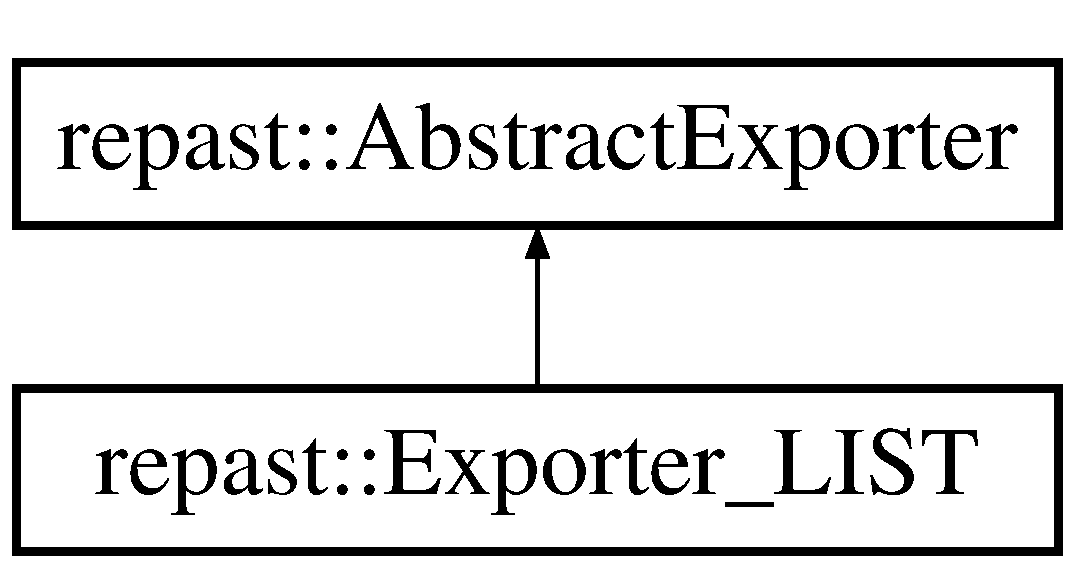
\includegraphics[height=2.000000cm]{classrepast_1_1_exporter___l_i_s_t}
\end{center}
\end{figure}
\subsection*{Public Member Functions}
\begin{DoxyCompactItemize}
\item 
\hypertarget{classrepast_1_1_exporter___l_i_s_t_af3ef5c07f5a8d1eb38c5b97727f92c9e}{virtual void \hyperlink{classrepast_1_1_exporter___l_i_s_t_af3ef5c07f5a8d1eb38c5b97727f92c9e}{register\-Incoming\-Requests} (std\-::vector$<$ \hyperlink{classrepast_1_1_agent_request}{Agent\-Request} $>$ \&requests)}\label{classrepast_1_1_exporter___l_i_s_t_af3ef5c07f5a8d1eb38c5b97727f92c9e}

\begin{DoxyCompactList}\small\item\em Makes a record of the data receives (in the form of a vector of Agent\-Requests) so that the agents' data can be sent to the requesting processes. \end{DoxyCompactList}\item 
\hypertarget{classrepast_1_1_exporter___l_i_s_t_a2df4abe8a73a23ec17bd02ec05833ec4}{{\bfseries Exporter\-\_\-\-L\-I\-S\-T} (Status\-Map $\ast$outgoing\-Status\-Map, \hyperlink{classrepast_1_1_agent_exporter_data}{Agent\-Exporter\-Data} $\ast$outgoing\-Agent\-Exporter\-Info)}\label{classrepast_1_1_exporter___l_i_s_t_a2df4abe8a73a23ec17bd02ec05833ec4}

\item 
\hypertarget{classrepast_1_1_exporter___l_i_s_t_a6b868c012bd5547d510f862c8bce620d}{virtual std\-::string \hyperlink{classrepast_1_1_exporter___l_i_s_t_a6b868c012bd5547d510f862c8bce620d}{get\-Report} ()}\label{classrepast_1_1_exporter___l_i_s_t_a6b868c012bd5547d510f862c8bce620d}

\begin{DoxyCompactList}\small\item\em Gets a printable report of the state of this object. \end{DoxyCompactList}\end{DoxyCompactItemize}
\subsection*{Additional Inherited Members}


\subsection{Detailed Description}
Maintains a list of agents being exported for each receiving process. 

An agent that is requested more than once will appear on this list more than once; canceling an agent just once removes only one of its appearances on this list. A 'send' will be created for a receiving process only if that process has entries in the list. 

The documentation for this class was generated from the following files\-:\begin{DoxyCompactItemize}
\item 
repast\-\_\-hpc/Agent\-Importer\-Exporter.\-h\item 
repast\-\_\-hpc/Agent\-Importer\-Exporter.\-cpp\end{DoxyCompactItemize}

\hypertarget{classrepast_1_1_exporter___s_e_t}{\section{repast\-:\-:Exporter\-\_\-\-S\-E\-T Class Reference}
\label{classrepast_1_1_exporter___s_e_t}\index{repast\-::\-Exporter\-\_\-\-S\-E\-T@{repast\-::\-Exporter\-\_\-\-S\-E\-T}}
}


Maintains a set of agents being exported for each receiving process.  




{\ttfamily \#include $<$Agent\-Importer\-Exporter.\-h$>$}

Inheritance diagram for repast\-:\-:Exporter\-\_\-\-S\-E\-T\-:\begin{figure}[H]
\begin{center}
\leavevmode
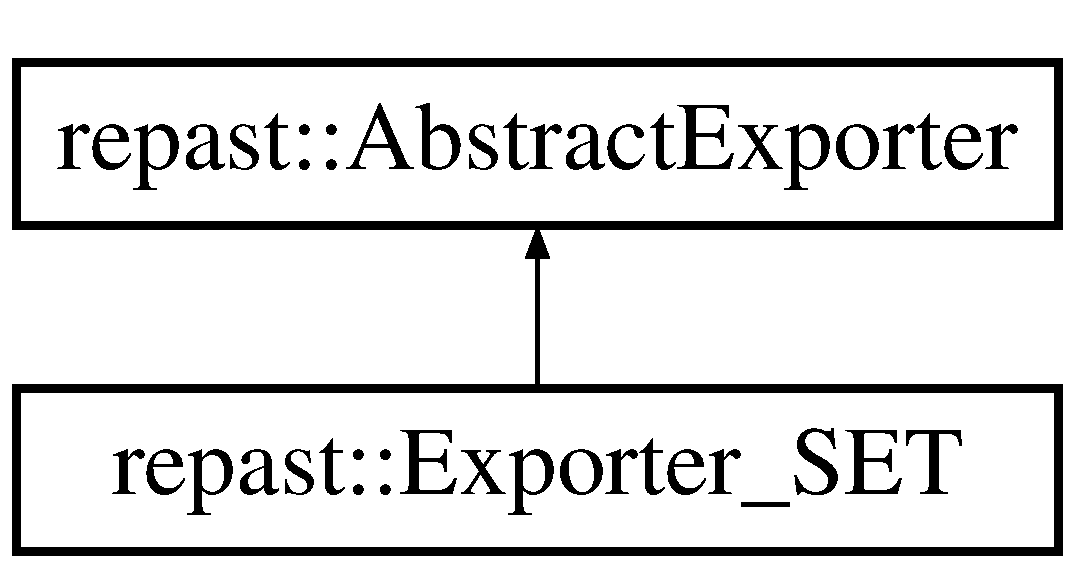
\includegraphics[height=2.000000cm]{classrepast_1_1_exporter___s_e_t}
\end{center}
\end{figure}
\subsection*{Public Member Functions}
\begin{DoxyCompactItemize}
\item 
\hypertarget{classrepast_1_1_exporter___s_e_t_a06463c5911250be6ac77c1c3b5f2ef34}{virtual void \hyperlink{classrepast_1_1_exporter___s_e_t_a06463c5911250be6ac77c1c3b5f2ef34}{register\-Incoming\-Requests} (std\-::vector$<$ \hyperlink{classrepast_1_1_agent_request}{Agent\-Request} $>$ \&requests)}\label{classrepast_1_1_exporter___s_e_t_a06463c5911250be6ac77c1c3b5f2ef34}

\begin{DoxyCompactList}\small\item\em Makes a record of the data receives (in the form of a vector of Agent\-Requests) so that the agents' data can be sent to the requesting processes. \end{DoxyCompactList}\item 
\hypertarget{classrepast_1_1_exporter___s_e_t_afb4b63299bb8a761dfc55dd9e4fec3d8}{{\bfseries Exporter\-\_\-\-S\-E\-T} (Status\-Map $\ast$outgoing\-Status\-Map, \hyperlink{classrepast_1_1_agent_exporter_data}{Agent\-Exporter\-Data} $\ast$outgoing\-Agent\-Exporter\-Info)}\label{classrepast_1_1_exporter___s_e_t_afb4b63299bb8a761dfc55dd9e4fec3d8}

\item 
\hypertarget{classrepast_1_1_exporter___s_e_t_a84d24e786b0048d12b789bfdf14d276f}{virtual std\-::string \hyperlink{classrepast_1_1_exporter___s_e_t_a84d24e786b0048d12b789bfdf14d276f}{get\-Report} ()}\label{classrepast_1_1_exporter___s_e_t_a84d24e786b0048d12b789bfdf14d276f}

\begin{DoxyCompactList}\small\item\em Gets a printable report of the state of this object. \end{DoxyCompactList}\end{DoxyCompactItemize}
\subsection*{Additional Inherited Members}


\subsection{Detailed Description}
Maintains a set of agents being exported for each receiving process. 

An agent that is requested more than once will appear in this set only once; canceling an agent just once removes it from this set. A 'send' will be created for a receiving process only if that process has entries in the list. 

The documentation for this class was generated from the following files\-:\begin{DoxyCompactItemize}
\item 
repast\-\_\-hpc/Agent\-Importer\-Exporter.\-h\item 
repast\-\_\-hpc/Agent\-Importer\-Exporter.\-cpp\end{DoxyCompactItemize}

\hypertarget{classrepast_1_1_export_request}{\section{repast\-:\-:Export\-Request Class Reference}
\label{classrepast_1_1_export_request}\index{repast\-::\-Export\-Request@{repast\-::\-Export\-Request}}
}


{\itshape D\-E\-P\-R\-E\-C\-A\-T\-E\-D} Used to send a request for agent information from another process  




{\ttfamily \#include $<$Shared\-Network.\-h$>$}

\subsection*{Public Member Functions}
\begin{DoxyCompactItemize}
\item 
\hypertarget{classrepast_1_1_export_request_a108d76019feb5c21b7c5560f5da130df}{{\bfseries Export\-Request} (int export\-To, \hyperlink{classrepast_1_1_agent_id}{Agent\-Id} id)}\label{classrepast_1_1_export_request_a108d76019feb5c21b7c5560f5da130df}

\item 
\hypertarget{classrepast_1_1_export_request_a4b3b905a6ee12870c7a729c1263698dc}{\hyperlink{classrepast_1_1_agent_id}{Agent\-Id} {\bfseries agent} () const }\label{classrepast_1_1_export_request_a4b3b905a6ee12870c7a729c1263698dc}

\item 
\hypertarget{classrepast_1_1_export_request_aa33de1bcdafc7cb636ba330c01255eb1}{int {\bfseries export\-To} ()}\label{classrepast_1_1_export_request_aa33de1bcdafc7cb636ba330c01255eb1}

\end{DoxyCompactItemize}
\subsection*{Friends}
\begin{DoxyCompactItemize}
\item 
\hypertarget{classrepast_1_1_export_request_ac98d07dd8f7b70e16ccb9a01abf56b9c}{class {\bfseries boost\-::serialization\-::access}}\label{classrepast_1_1_export_request_ac98d07dd8f7b70e16ccb9a01abf56b9c}

\end{DoxyCompactItemize}


\subsection{Detailed Description}
{\itshape D\-E\-P\-R\-E\-C\-A\-T\-E\-D} Used to send a request for agent information from another process 

\begin{DoxyRefDesc}{Deprecated}
\item[\hyperlink{deprecated__deprecated000003}{Deprecated}]As of Version 2.\-0 \end{DoxyRefDesc}


The documentation for this class was generated from the following files\-:\begin{DoxyCompactItemize}
\item 
repast\-\_\-hpc/Shared\-Network.\-h\item 
repast\-\_\-hpc/Shared\-Network.\-cpp\end{DoxyCompactItemize}

\hypertarget{structrepast_1_1_extract_ptrs}{\section{repast\-:\-:Extract\-Ptrs$<$ T $>$ Struct Template Reference}
\label{structrepast_1_1_extract_ptrs}\index{repast\-::\-Extract\-Ptrs$<$ T $>$@{repast\-::\-Extract\-Ptrs$<$ T $>$}}
}


Unary function that allows retrieving the occupants of locations.  




{\ttfamily \#include $<$Multiple\-Occupancy.\-h$>$}

Inheritance diagram for repast\-:\-:Extract\-Ptrs$<$ T $>$\-:\begin{figure}[H]
\begin{center}
\leavevmode
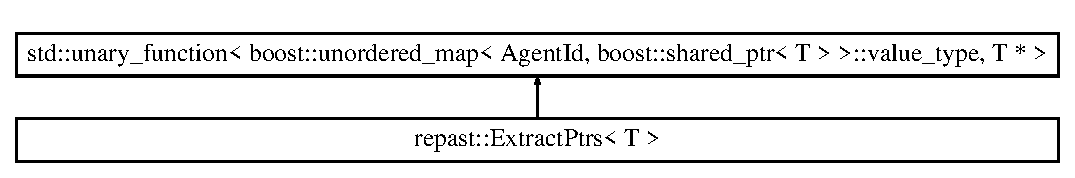
\includegraphics[height=1.944445cm]{structrepast_1_1_extract_ptrs}
\end{center}
\end{figure}
\subsection*{Public Member Functions}
\begin{DoxyCompactItemize}
\item 
\hypertarget{structrepast_1_1_extract_ptrs_a5f865f44030fee1a36179d9121841b9d}{T $\ast$ {\bfseries operator()} (typename boost\-::unordered\-\_\-map$<$ \hyperlink{classrepast_1_1_agent_id}{Agent\-Id}, boost\-::shared\-\_\-ptr$<$ T $>$ $>$\-::value\-\_\-type \&val)}\label{structrepast_1_1_extract_ptrs_a5f865f44030fee1a36179d9121841b9d}

\end{DoxyCompactItemize}


\subsection{Detailed Description}
\subsubsection*{template$<$typename T$>$struct repast\-::\-Extract\-Ptrs$<$ T $>$}

Unary function that allows retrieving the occupants of locations. 

The documentation for this struct was generated from the following file\-:\begin{DoxyCompactItemize}
\item 
repast\-\_\-hpc/Multiple\-Occupancy.\-h\end{DoxyCompactItemize}

\hypertarget{classrepast_1_1_functor}{\section{repast\-:\-:Functor Class Reference}
\label{classrepast_1_1_functor}\index{repast\-::\-Functor@{repast\-::\-Functor}}
}


\hyperlink{classrepast_1_1_functor}{Functor} interface.  




{\ttfamily \#include $<$Schedule.\-h$>$}

Inheritance diagram for repast\-:\-:Functor\-:\begin{figure}[H]
\begin{center}
\leavevmode
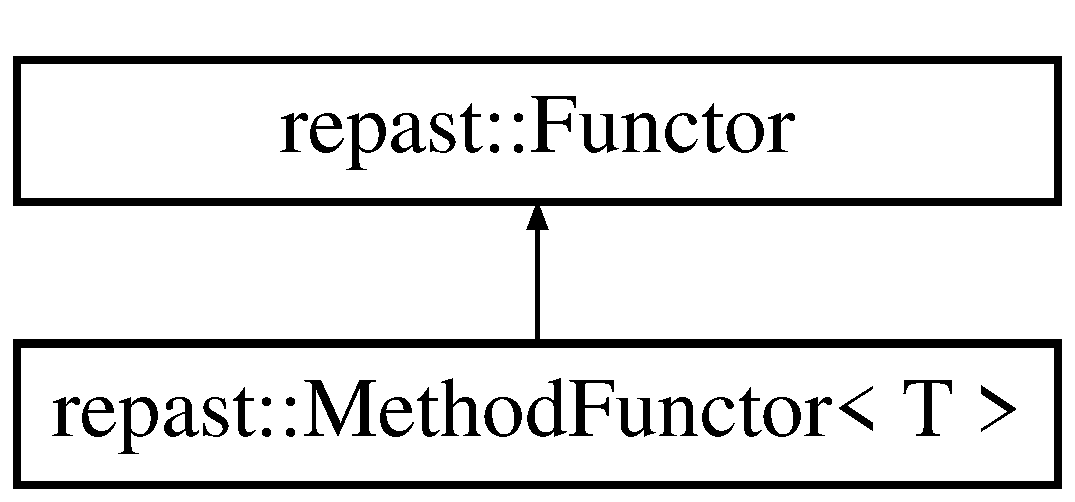
\includegraphics[height=2.000000cm]{classrepast_1_1_functor}
\end{center}
\end{figure}
\subsection*{Public Member Functions}
\begin{DoxyCompactItemize}
\item 
\hypertarget{classrepast_1_1_functor_adadfddb7b4d7da5f105287498ff4d7d8}{virtual void {\bfseries operator()} ()=0}\label{classrepast_1_1_functor_adadfddb7b4d7da5f105287498ff4d7d8}

\end{DoxyCompactItemize}


\subsection{Detailed Description}
\hyperlink{classrepast_1_1_functor}{Functor} interface. 

The documentation for this class was generated from the following files\-:\begin{DoxyCompactItemize}
\item 
repast\-\_\-hpc/Schedule.\-h\item 
repast\-\_\-hpc/Schedule.\-cpp\end{DoxyCompactItemize}

\hypertarget{classrepast_1_1_graph}{\section{repast\-:\-:Graph$<$ V, E, Ec, Ec\-M $>$ Class Template Reference}
\label{classrepast_1_1_graph}\index{repast\-::\-Graph$<$ V, E, Ec, Ec\-M $>$@{repast\-::\-Graph$<$ V, E, Ec, Ec\-M $>$}}
}


\hyperlink{classrepast_1_1_graph}{Graph} / Network implementation where agents are vertices in the graph.  




{\ttfamily \#include $<$Graph.\-h$>$}

Inheritance diagram for repast\-:\-:Graph$<$ V, E, Ec, Ec\-M $>$\-:\begin{figure}[H]
\begin{center}
\leavevmode
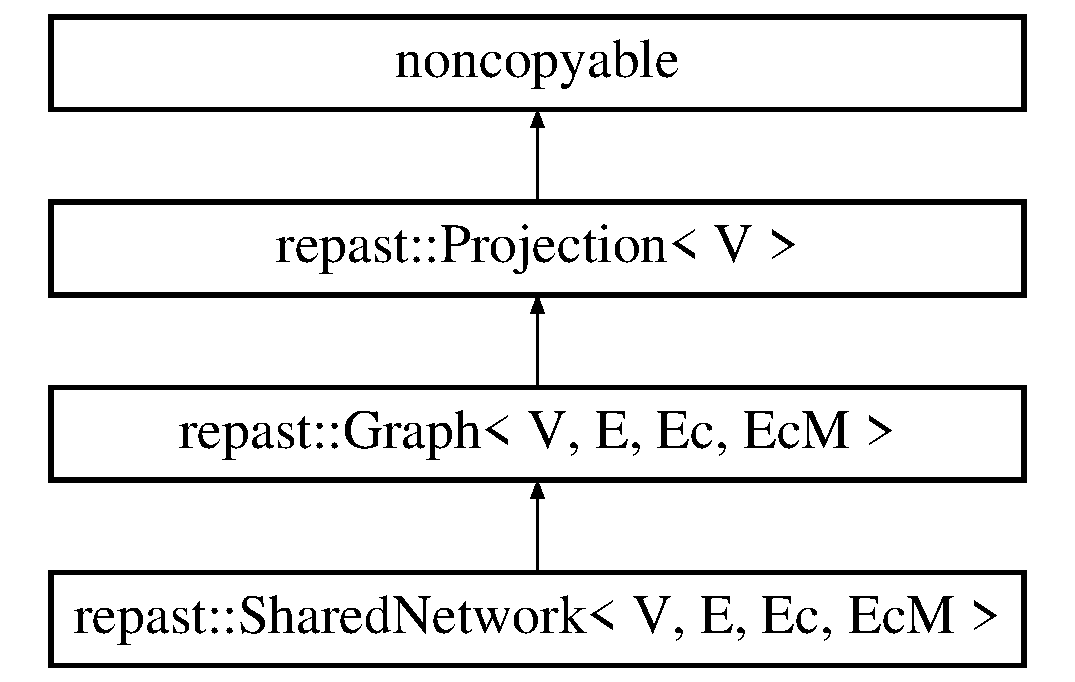
\includegraphics[height=4.000000cm]{classrepast_1_1_graph}
\end{center}
\end{figure}
\subsection*{Public Types}
\begin{DoxyCompactItemize}
\item 
\hypertarget{classrepast_1_1_graph_acee609459f11e02371ae4d8d226aafab}{typedef \\*
boost\-::transform\-\_\-iterator\\*
$<$ \hyperlink{structrepast_1_1_node_getter}{Node\-Getter}$<$ V, E $>$, typename \\*
Vertex\-Map\-::const\-\_\-iterator $>$ \hyperlink{classrepast_1_1_graph_acee609459f11e02371ae4d8d226aafab}{vertex\-\_\-iterator}}\label{classrepast_1_1_graph_acee609459f11e02371ae4d8d226aafab}

\begin{DoxyCompactList}\small\item\em An iterator over the agents that are the vertices in this \hyperlink{classrepast_1_1_graph}{Graph}. \end{DoxyCompactList}\end{DoxyCompactItemize}
\subsection*{Public Member Functions}
\begin{DoxyCompactItemize}
\item 
\hyperlink{classrepast_1_1_graph_ae2a9ad624d6fd581450243cd49e4ffe2}{Graph} (std\-::string \hyperlink{classrepast_1_1_projection_ab60a0ab4f584685780307d7431b61800}{name}, bool directed, Ec\-M $\ast$edge\-Content\-Mgr)
\begin{DoxyCompactList}\small\item\em Creates a \hyperlink{classrepast_1_1_graph}{Graph} with the specified name. \end{DoxyCompactList}\item 
\hypertarget{classrepast_1_1_graph_ad9e5b7105b55f1e967dff196e83a1621}{\hyperlink{classrepast_1_1_graph_ad9e5b7105b55f1e967dff196e83a1621}{Graph} (const \hyperlink{classrepast_1_1_graph}{Graph}$<$ V, E, Ec, Ec\-M $>$ \&graph)}\label{classrepast_1_1_graph_ad9e5b7105b55f1e967dff196e83a1621}

\begin{DoxyCompactList}\small\item\em Copy constructor for the graph. \end{DoxyCompactList}\item 
\hypertarget{classrepast_1_1_graph_a2404ed301bcecb8af4d1d45bd5de4c8a}{\hyperlink{classrepast_1_1_graph}{Graph} \& {\bfseries operator=} (const \hyperlink{classrepast_1_1_graph}{Graph} \&graph)}\label{classrepast_1_1_graph_a2404ed301bcecb8af4d1d45bd5de4c8a}

\item 
virtual boost\-::shared\-\_\-ptr$<$ E $>$ \hyperlink{classrepast_1_1_graph_a7ce027bc5e1c0119f9cce87aadf49bb7}{add\-Edge} (V $\ast$source, V $\ast$target)
\begin{DoxyCompactList}\small\item\em Adds an edge between source and target to this \hyperlink{classrepast_1_1_graph}{Graph}. \end{DoxyCompactList}\item 
virtual boost\-::shared\-\_\-ptr$<$ E $>$ \hyperlink{classrepast_1_1_graph_a9cc7843398086080c064123aaf245dd5}{add\-Edge} (V $\ast$source, V $\ast$target, double weight)
\begin{DoxyCompactList}\small\item\em Adds an edge with the specified weight between source and target to this \hyperlink{classrepast_1_1_graph}{Graph}. \end{DoxyCompactList}\item 
virtual boost\-::shared\-\_\-ptr$<$ E $>$ \hyperlink{classrepast_1_1_graph_a160050d2b0ce64a59b32c2697ddd622b}{find\-Edge} (V $\ast$source, V $\ast$target)
\begin{DoxyCompactList}\small\item\em Gets the edge between the source and target or 0 if no such edge is found. \end{DoxyCompactList}\item 
virtual void \hyperlink{classrepast_1_1_graph_a9d6eb280c2a2034f127453c5f965d61e}{successors} (V $\ast$vertex, std\-::vector$<$ V $\ast$ $>$ \&out)
\begin{DoxyCompactList}\small\item\em Gets the sucessors of the specified vertex and puts them in out. \end{DoxyCompactList}\item 
virtual void \hyperlink{classrepast_1_1_graph_a9686c8fee74dbcb6b5bd0ddc9cc82827}{predecessors} (V $\ast$vertex, std\-::vector$<$ V $\ast$ $>$ \&out)
\begin{DoxyCompactList}\small\item\em Gets the predecessors of the specified vertex and puts them in out. \end{DoxyCompactList}\item 
virtual void \hyperlink{classrepast_1_1_graph_ac07ec9433947d5c677786e37e4cb0973}{adjacent} (V $\ast$vertex, std\-::vector$<$ V $\ast$ $>$ \&out)
\begin{DoxyCompactList}\small\item\em Gets all the agent adjacent to the specified vertex. \end{DoxyCompactList}\item 
virtual void \hyperlink{classrepast_1_1_graph_a95ddd223fa26a5390c13aa1c4fec9254}{remove\-Edge} (V $\ast$source, V $\ast$target)
\begin{DoxyCompactList}\small\item\em Removes the edge between source and target from this \hyperlink{classrepast_1_1_graph}{Graph}. \end{DoxyCompactList}\item 
virtual void \hyperlink{classrepast_1_1_graph_a159360404f97fd8a7339ca98d13151cb}{remove\-Edge} (const \hyperlink{classrepast_1_1_agent_id}{Agent\-Id} \&source, const \hyperlink{classrepast_1_1_agent_id}{Agent\-Id} \&target)
\begin{DoxyCompactList}\small\item\em Removes the edge between source and target from this \hyperlink{classrepast_1_1_graph}{Graph}. \end{DoxyCompactList}\item 
virtual int \hyperlink{classrepast_1_1_graph_a00f9c58855d8ba8ca197f695fdf5c6cc}{in\-Degree} (V $\ast$vertex)
\begin{DoxyCompactList}\small\item\em Gets the in-\/degree of the specified vertex. \end{DoxyCompactList}\item 
virtual int \hyperlink{classrepast_1_1_graph_aeca552decfd6069f132613c1f5aab59d}{out\-Degree} (V $\ast$vertex)
\begin{DoxyCompactList}\small\item\em Gets the out-\/degree of the specified vertex. \end{DoxyCompactList}\item 
int \hyperlink{classrepast_1_1_graph_aaf15eede1ff417d8164f0eb4825cad09}{edge\-Count} () const 
\begin{DoxyCompactList}\small\item\em Gets the number of edges in this \hyperlink{classrepast_1_1_graph}{Graph}. \end{DoxyCompactList}\item 
int \hyperlink{classrepast_1_1_graph_ae9e0b0fc607154387d60596465c8fb80}{vertex\-Count} () const 
\begin{DoxyCompactList}\small\item\em Gets the number of vertices in this \hyperlink{classrepast_1_1_graph}{Graph}. \end{DoxyCompactList}\item 
\hyperlink{classrepast_1_1_graph_acee609459f11e02371ae4d8d226aafab}{vertex\-\_\-iterator} \hyperlink{classrepast_1_1_graph_abbc3dafd7087984a83ac0190e5058c5b}{vertices\-Begin} ()
\begin{DoxyCompactList}\small\item\em Gets the start of an iterator over all the vertices in this graph. \end{DoxyCompactList}\item 
\hyperlink{classrepast_1_1_graph_acee609459f11e02371ae4d8d226aafab}{vertex\-\_\-iterator} \hyperlink{classrepast_1_1_graph_acd76c847169c86e1e981100e8cf896f0}{vertices\-End} ()
\begin{DoxyCompactList}\small\item\em Gets the end of an iterator over all the vertices in this graph. \end{DoxyCompactList}\item 
\hypertarget{classrepast_1_1_graph_a2bfd1ab5fde73c290df15318746831f5}{void {\bfseries show\-Edges} ()}\label{classrepast_1_1_graph_a2bfd1ab5fde73c290df15318746831f5}

\item 
\hypertarget{classrepast_1_1_graph_a8c2f3ff6eb7d2975ed29cadcdd532b49}{virtual bool {\bfseries is\-Master} (E $\ast$e)=0}\label{classrepast_1_1_graph_a8c2f3ff6eb7d2975ed29cadcdd532b49}

\item 
virtual bool \hyperlink{classrepast_1_1_graph_aedaa8e44eb04056df2acabbeba373201}{keeps\-Agents\-On\-Sync\-Proj} ()
\begin{DoxyCompactList}\small\item\em Should return true if the \hyperlink{classrepast_1_1_projection}{Projection} implemented can 'keep' some (non-\/local) agents during a projection information synchronization operation. \end{DoxyCompactList}\item 
virtual bool \hyperlink{classrepast_1_1_graph_a80cd467aae6d5e2c381bbe9cade6cbba}{sends\-Secondary\-Agents\-On\-Status\-Exchange} ()
\begin{DoxyCompactList}\small\item\em Should return true if the \hyperlink{classrepast_1_1_projection}{Projection} implemented will send secondary agents during a status exchange. \end{DoxyCompactList}\item 
virtual void \hyperlink{classrepast_1_1_graph_ab4200382f280c05f020611428507a134}{get\-Info\-Exchange\-Partners} (std\-::set$<$ int $>$ \&ps\-To\-Send\-To, std\-::set$<$ int $>$ \&ps\-To\-Receive\-From)
\begin{DoxyCompactList}\small\item\em Gets the set of processes with which this \hyperlink{classrepast_1_1_projection}{Projection} exchanges projection info. \end{DoxyCompactList}\item 
virtual void \hyperlink{classrepast_1_1_graph_a3e9a52d6d45473260e2771fe426c8a15}{get\-Agent\-Status\-Exchange\-Partners} (std\-::set$<$ int $>$ \&ps\-To\-Send\-To, std\-::set$<$ int $>$ \&ps\-To\-Receive\-From)
\begin{DoxyCompactList}\small\item\em Gets the set of processes with which this \hyperlink{classrepast_1_1_projection}{Projection} exchanges agent status info-\/ that is, the set of processes from which agents can move to this one or to which they can move when moving from this one. \end{DoxyCompactList}\item 
\hypertarget{classrepast_1_1_graph_ad3cffccc052f93d644a0d58630577ea0}{virtual void \hyperlink{classrepast_1_1_graph_ad3cffccc052f93d644a0d58630577ea0}{get\-Projection\-Info} (std\-::vector$<$ \hyperlink{classrepast_1_1_agent_id}{Agent\-Id} $>$ \&agents, std\-::vector$<$ \hyperlink{classrepast_1_1_projection_info_packet}{Projection\-Info\-Packet} $\ast$ $>$ \&packets, bool secondary\-Info=false, std\-::set$<$ \hyperlink{classrepast_1_1_agent_id}{Agent\-Id} $>$ $\ast$secondary\-Ids=0, int dest\-Proc=-\/1)}\label{classrepast_1_1_graph_ad3cffccc052f93d644a0d58630577ea0}

\begin{DoxyCompactList}\small\item\em Convenience wrapper that gets all of the projection information for the agents specified (calls implementation in child class that gets only the information for one agent). \end{DoxyCompactList}\item 
\hypertarget{classrepast_1_1_graph_acd792216213093f9fea3b676d10ccdc7}{virtual \hyperlink{classrepast_1_1_projection_info_packet}{Projection\-Info\-Packet} $\ast$ {\bfseries get\-Projection\-Info} (\hyperlink{classrepast_1_1_agent_id}{Agent\-Id} id, bool secondary\-Info=false, std\-::set$<$ \hyperlink{classrepast_1_1_agent_id}{Agent\-Id} $>$ $\ast$secondary\-Ids=0, int dest\-Proc=-\/1)}\label{classrepast_1_1_graph_acd792216213093f9fea3b676d10ccdc7}

\item 
\hypertarget{classrepast_1_1_graph_ad1a011ae319ca66af55a4131e3ce7804}{virtual void {\bfseries update\-Projection\-Info} (\hyperlink{classrepast_1_1_projection_info_packet}{Projection\-Info\-Packet} $\ast$pip, \hyperlink{classrepast_1_1_context}{Context}$<$ V $>$ $\ast$context)}\label{classrepast_1_1_graph_ad1a011ae319ca66af55a4131e3ce7804}

\item 
\hypertarget{classrepast_1_1_graph_af53ecedb239116dfe1a978fdfb1d364c}{virtual void {\bfseries get\-Required\-Agents} (std\-::set$<$ \hyperlink{classrepast_1_1_agent_id}{Agent\-Id} $>$ \&agents\-To\-Test, std\-::set$<$ \hyperlink{classrepast_1_1_agent_id}{Agent\-Id} $>$ \&agents\-Required, R\-A\-D\-I\-U\-S radius=\hyperlink{classrepast_1_1_projection}{Projection}$<$ V $>$\-::P\-R\-I\-M\-A\-R\-Y)}\label{classrepast_1_1_graph_af53ecedb239116dfe1a978fdfb1d364c}

\item 
virtual void \hyperlink{classrepast_1_1_graph_a011c1f0f065e5b8238c6783966c380eb}{get\-Agents\-To\-Push} (std\-::set$<$ \hyperlink{classrepast_1_1_agent_id}{Agent\-Id} $>$ \&agents\-To\-Test, std\-::map$<$ int, std\-::set$<$ \hyperlink{classrepast_1_1_agent_id}{Agent\-Id} $>$ $>$ \&agents\-To\-Push)
\begin{DoxyCompactList}\small\item\em Given a set of agents, gets the agents that this projection implementation must 'push' to other processes. \end{DoxyCompactList}\item 
\hypertarget{classrepast_1_1_graph_a2fa24c44da950218515a28a9ebae26c0}{virtual void {\bfseries clean\-Projection\-Info} (std\-::set$<$ \hyperlink{classrepast_1_1_agent_id}{Agent\-Id} $>$ \&agents\-To\-Keep)}\label{classrepast_1_1_graph_a2fa24c44da950218515a28a9ebae26c0}

\item 
\hypertarget{classrepast_1_1_graph_aae3c1f6c8031633d866eed178b5556e7}{void {\bfseries clear\-Conflicted\-Edges} ()}\label{classrepast_1_1_graph_aae3c1f6c8031633d866eed178b5556e7}

\item 
\hypertarget{classrepast_1_1_graph_a4ecd9032c3380032e5e387b421540b72}{void {\bfseries get\-Conflicted\-Edges} (std\-::set$<$ boost\-::shared\-\_\-ptr$<$ E $>$ $>$ \&conflicted\-Edges)}\label{classrepast_1_1_graph_a4ecd9032c3380032e5e387b421540b72}

\end{DoxyCompactItemize}
\subsection*{Public Attributes}
\begin{DoxyCompactItemize}
\item 
\hypertarget{classrepast_1_1_graph_a26a275229c943860f7dcc8f12a819d51}{std\-::set$<$ int $>$ {\bfseries ranks\-To\-Send\-Proj\-Info\-To}}\label{classrepast_1_1_graph_a26a275229c943860f7dcc8f12a819d51}

\item 
\hypertarget{classrepast_1_1_graph_ac6bd3c93bc7fc980daee32416c62cef5}{std\-::set$<$ int $>$ {\bfseries ranks\-To\-Receive\-Proj\-Info\-From}}\label{classrepast_1_1_graph_ac6bd3c93bc7fc980daee32416c62cef5}

\item 
\hypertarget{classrepast_1_1_graph_af6ffbf7aafeaa71373c833215d6e7361}{std\-::set$<$ int $>$ {\bfseries ranks\-To\-Send\-Agent\-Status\-Info\-To}}\label{classrepast_1_1_graph_af6ffbf7aafeaa71373c833215d6e7361}

\item 
\hypertarget{classrepast_1_1_graph_ab6aa89bc4355dc7be2e9ffcf4831b69e}{std\-::set$<$ int $>$ {\bfseries ranks\-To\-Receive\-Agent\-Status\-Info\-From}}\label{classrepast_1_1_graph_ab6aa89bc4355dc7be2e9ffcf4831b69e}

\item 
\hypertarget{classrepast_1_1_graph_a71df0c0ac35f4464ff6d72f70bead983}{bool {\bfseries keeps\-Agents}}\label{classrepast_1_1_graph_a71df0c0ac35f4464ff6d72f70bead983}

\item 
\hypertarget{classrepast_1_1_graph_accec73ce11057ca4b5019b3693e93354}{bool {\bfseries sends\-Secondary\-Agents}}\label{classrepast_1_1_graph_accec73ce11057ca4b5019b3693e93354}

\end{DoxyCompactItemize}
\subsection*{Protected Types}
\begin{DoxyCompactItemize}
\item 
\hypertarget{classrepast_1_1_graph_a8d44d7ffee81310e667905eb64798228}{typedef boost\-::unordered\-\_\-map\\*
$<$ \hyperlink{classrepast_1_1_agent_id}{Agent\-Id}, \hyperlink{classrepast_1_1_vertex}{Vertex}$<$ V, E $>$\\*
 $\ast$, \hyperlink{structrepast_1_1_hash_id}{Hash\-Id} $>$ {\bfseries Vertex\-Map}}\label{classrepast_1_1_graph_a8d44d7ffee81310e667905eb64798228}

\item 
\hypertarget{classrepast_1_1_graph_aeb3e3741243a80c9d3732805b018ed00}{typedef Vertex\-Map\-::iterator {\bfseries Vertex\-Map\-Iterator}}\label{classrepast_1_1_graph_aeb3e3741243a80c9d3732805b018ed00}

\item 
\hypertarget{classrepast_1_1_graph_a1c3c8e5132aa39f51bf64440e34f3e5c}{typedef \hyperlink{classrepast_1_1_projection}{Projection}$<$ V $>$\-::R\-A\-D\-I\-U\-S {\bfseries R\-A\-D\-I\-U\-S}}\label{classrepast_1_1_graph_a1c3c8e5132aa39f51bf64440e34f3e5c}

\end{DoxyCompactItemize}
\subsection*{Protected Member Functions}
\begin{DoxyCompactItemize}
\item 
\hypertarget{classrepast_1_1_graph_ac355b765b3ebcaafb62603ded91fb170}{void {\bfseries clean\-Up} ()}\label{classrepast_1_1_graph_ac355b765b3ebcaafb62603ded91fb170}

\item 
\hypertarget{classrepast_1_1_graph_abb88d9a266f2dde1782f62f221479314}{void {\bfseries init} (const \hyperlink{classrepast_1_1_graph}{Graph} \&graph)}\label{classrepast_1_1_graph_abb88d9a266f2dde1782f62f221479314}

\item 
\hypertarget{classrepast_1_1_graph_aab6a71c186e6acbe4e04dcd1a866712d}{virtual bool {\bfseries add\-Agent} (boost\-::shared\-\_\-ptr$<$ V $>$ agent)}\label{classrepast_1_1_graph_aab6a71c186e6acbe4e04dcd1a866712d}

\item 
\hypertarget{classrepast_1_1_graph_a437e50a2ca1330b1bd3d582cf711b628}{virtual void {\bfseries remove\-Agent} (V $\ast$agent)}\label{classrepast_1_1_graph_a437e50a2ca1330b1bd3d582cf711b628}

\item 
\hypertarget{classrepast_1_1_graph_a83187d1adf22e412f871102f5883df22}{virtual void {\bfseries do\-Add\-Edge} (boost\-::shared\-\_\-ptr$<$ E $>$ edge, bool allow\-Overwrite=true)}\label{classrepast_1_1_graph_a83187d1adf22e412f871102f5883df22}

\end{DoxyCompactItemize}
\subsection*{Protected Attributes}
\begin{DoxyCompactItemize}
\item 
\hypertarget{classrepast_1_1_graph_a4cf91f79bf224e8550d31a500fc2a47a}{int {\bfseries edge\-Count\-\_\-}}\label{classrepast_1_1_graph_a4cf91f79bf224e8550d31a500fc2a47a}

\item 
\hypertarget{classrepast_1_1_graph_a31bc527fc394104d5d2252d7302e8bff}{bool {\bfseries is\-Directed}}\label{classrepast_1_1_graph_a31bc527fc394104d5d2252d7302e8bff}

\item 
\hypertarget{classrepast_1_1_graph_a12f010263d0a805926ff66e54dbd8ae5}{Vertex\-Map {\bfseries vertices}}\label{classrepast_1_1_graph_a12f010263d0a805926ff66e54dbd8ae5}

\item 
\hypertarget{classrepast_1_1_graph_ab4cab2042913e901d8a9eb2c170da6de}{Ec\-M $\ast$ {\bfseries edge\-Content\-Manager}}\label{classrepast_1_1_graph_ab4cab2042913e901d8a9eb2c170da6de}

\end{DoxyCompactItemize}


\subsection{Detailed Description}
\subsubsection*{template$<$typename V, typename E, typename Ec, typename Ec\-M$>$class repast\-::\-Graph$<$ V, E, Ec, Ec\-M $>$}

\hyperlink{classrepast_1_1_graph}{Graph} / Network implementation where agents are vertices in the graph. 


\begin{DoxyTemplParams}{Template Parameters}
{\em V} & the type agents in the graph. This type should extend \hyperlink{classrepast_1_1_agent}{repast\-::\-Agent} \\
\hline
{\em E} & the edge type of the graph. This type should extend \hyperlink{classrepast_1_1_repast_edge}{repast\-::\-Repast\-Edge}. \\
\hline
{\em Ec} & class of serializable Edge Content \\
\hline
{\em Ec\-M} & Class that is capable of transforming an Edge into Edge Content and vice versa \\
\hline
\end{DoxyTemplParams}


\subsection{Constructor \& Destructor Documentation}
\hypertarget{classrepast_1_1_graph_ae2a9ad624d6fd581450243cd49e4ffe2}{\index{repast\-::\-Graph@{repast\-::\-Graph}!Graph@{Graph}}
\index{Graph@{Graph}!repast::Graph@{repast\-::\-Graph}}
\subsubsection[{Graph}]{\setlength{\rightskip}{0pt plus 5cm}template$<$typename V, typename E, typename Ec, typename Ec\-M$>$ {\bf repast\-::\-Graph}$<$ V, E, Ec, Ec\-M $>$\-::{\bf Graph} (
\begin{DoxyParamCaption}
\item[{std\-::string}]{name, }
\item[{bool}]{directed, }
\item[{Ec\-M $\ast$}]{edge\-Content\-Mgr}
\end{DoxyParamCaption}
)\hspace{0.3cm}{\ttfamily [inline]}}}\label{classrepast_1_1_graph_ae2a9ad624d6fd581450243cd49e4ffe2}


Creates a \hyperlink{classrepast_1_1_graph}{Graph} with the specified name. 


\begin{DoxyParams}{Parameters}
{\em name} & the name of the graph \\
\hline
{\em directed} & whether or not the created \hyperlink{classrepast_1_1_graph}{Graph} is directed \\
\hline
\end{DoxyParams}


\subsection{Member Function Documentation}
\hypertarget{classrepast_1_1_graph_a7ce027bc5e1c0119f9cce87aadf49bb7}{\index{repast\-::\-Graph@{repast\-::\-Graph}!add\-Edge@{add\-Edge}}
\index{add\-Edge@{add\-Edge}!repast::Graph@{repast\-::\-Graph}}
\subsubsection[{add\-Edge}]{\setlength{\rightskip}{0pt plus 5cm}template$<$typename V , typename E , typename Ec , typename Ec\-M $>$ boost\-::shared\-\_\-ptr$<$ E $>$ {\bf repast\-::\-Graph}$<$ V, E, Ec, Ec\-M $>$\-::add\-Edge (
\begin{DoxyParamCaption}
\item[{V $\ast$}]{source, }
\item[{V $\ast$}]{target}
\end{DoxyParamCaption}
)\hspace{0.3cm}{\ttfamily [virtual]}}}\label{classrepast_1_1_graph_a7ce027bc5e1c0119f9cce87aadf49bb7}


Adds an edge between source and target to this \hyperlink{classrepast_1_1_graph}{Graph}. 


\begin{DoxyParams}{Parameters}
{\em source} & the source of the edge \\
\hline
{\em target} & the target of the edge\\
\hline
\end{DoxyParams}
\begin{DoxyReturn}{Returns}
the added edge. 
\end{DoxyReturn}
\hypertarget{classrepast_1_1_graph_a9cc7843398086080c064123aaf245dd5}{\index{repast\-::\-Graph@{repast\-::\-Graph}!add\-Edge@{add\-Edge}}
\index{add\-Edge@{add\-Edge}!repast::Graph@{repast\-::\-Graph}}
\subsubsection[{add\-Edge}]{\setlength{\rightskip}{0pt plus 5cm}template$<$typename V , typename E , typename Ec , typename Ec\-M $>$ boost\-::shared\-\_\-ptr$<$ E $>$ {\bf repast\-::\-Graph}$<$ V, E, Ec, Ec\-M $>$\-::add\-Edge (
\begin{DoxyParamCaption}
\item[{V $\ast$}]{source, }
\item[{V $\ast$}]{target, }
\item[{double}]{weight}
\end{DoxyParamCaption}
)\hspace{0.3cm}{\ttfamily [virtual]}}}\label{classrepast_1_1_graph_a9cc7843398086080c064123aaf245dd5}


Adds an edge with the specified weight between source and target to this \hyperlink{classrepast_1_1_graph}{Graph}. 


\begin{DoxyParams}{Parameters}
{\em source} & the source of the edge \\
\hline
{\em target} & the target of the edge \\
\hline
{\em weight} & the weight of the edge\\
\hline
\end{DoxyParams}
\begin{DoxyReturn}{Returns}
the added edge. 
\end{DoxyReturn}
\hypertarget{classrepast_1_1_graph_ac07ec9433947d5c677786e37e4cb0973}{\index{repast\-::\-Graph@{repast\-::\-Graph}!adjacent@{adjacent}}
\index{adjacent@{adjacent}!repast::Graph@{repast\-::\-Graph}}
\subsubsection[{adjacent}]{\setlength{\rightskip}{0pt plus 5cm}template$<$typename V , typename E , typename Ec , typename Ec\-M $>$ void {\bf repast\-::\-Graph}$<$ V, E, Ec, Ec\-M $>$\-::adjacent (
\begin{DoxyParamCaption}
\item[{V $\ast$}]{vertex, }
\item[{std\-::vector$<$ V $\ast$ $>$ \&}]{out}
\end{DoxyParamCaption}
)\hspace{0.3cm}{\ttfamily [virtual]}}}\label{classrepast_1_1_graph_ac07ec9433947d5c677786e37e4cb0973}


Gets all the agent adjacent to the specified vertex. 


\begin{DoxyParams}[1]{Parameters}
 & {\em vertex} & the vertex whose adjacent agents we want to get \\
\hline
\mbox{\tt out}  & {\em the} & vector where the results will be put \\
\hline
\end{DoxyParams}
\hypertarget{classrepast_1_1_graph_aaf15eede1ff417d8164f0eb4825cad09}{\index{repast\-::\-Graph@{repast\-::\-Graph}!edge\-Count@{edge\-Count}}
\index{edge\-Count@{edge\-Count}!repast::Graph@{repast\-::\-Graph}}
\subsubsection[{edge\-Count}]{\setlength{\rightskip}{0pt plus 5cm}template$<$typename V, typename E, typename Ec, typename Ec\-M$>$ int {\bf repast\-::\-Graph}$<$ V, E, Ec, Ec\-M $>$\-::edge\-Count (
\begin{DoxyParamCaption}
{}
\end{DoxyParamCaption}
) const\hspace{0.3cm}{\ttfamily [inline]}}}\label{classrepast_1_1_graph_aaf15eede1ff417d8164f0eb4825cad09}


Gets the number of edges in this \hyperlink{classrepast_1_1_graph}{Graph}. 

\begin{DoxyReturn}{Returns}
the number of edges in this \hyperlink{classrepast_1_1_graph}{Graph}. 
\end{DoxyReturn}
\hypertarget{classrepast_1_1_graph_a160050d2b0ce64a59b32c2697ddd622b}{\index{repast\-::\-Graph@{repast\-::\-Graph}!find\-Edge@{find\-Edge}}
\index{find\-Edge@{find\-Edge}!repast::Graph@{repast\-::\-Graph}}
\subsubsection[{find\-Edge}]{\setlength{\rightskip}{0pt plus 5cm}template$<$typename V , typename E , typename Ec , typename Ec\-M $>$ boost\-::shared\-\_\-ptr$<$ E $>$ {\bf repast\-::\-Graph}$<$ V, E, Ec, Ec\-M $>$\-::find\-Edge (
\begin{DoxyParamCaption}
\item[{V $\ast$}]{source, }
\item[{V $\ast$}]{target}
\end{DoxyParamCaption}
)\hspace{0.3cm}{\ttfamily [virtual]}}}\label{classrepast_1_1_graph_a160050d2b0ce64a59b32c2697ddd622b}


Gets the edge between the source and target or 0 if no such edge is found. 


\begin{DoxyParams}{Parameters}
{\em source} & the source of the edge to find \\
\hline
{\em target} & the target of the edge to find\\
\hline
\end{DoxyParams}
\begin{DoxyReturn}{Returns}
the found edge or 0. 
\end{DoxyReturn}
\hypertarget{classrepast_1_1_graph_a3e9a52d6d45473260e2771fe426c8a15}{\index{repast\-::\-Graph@{repast\-::\-Graph}!get\-Agent\-Status\-Exchange\-Partners@{get\-Agent\-Status\-Exchange\-Partners}}
\index{get\-Agent\-Status\-Exchange\-Partners@{get\-Agent\-Status\-Exchange\-Partners}!repast::Graph@{repast\-::\-Graph}}
\subsubsection[{get\-Agent\-Status\-Exchange\-Partners}]{\setlength{\rightskip}{0pt plus 5cm}template$<$typename V , typename E , typename Ec , typename Ec\-M $>$ void {\bf repast\-::\-Graph}$<$ V, E, Ec, Ec\-M $>$\-::get\-Agent\-Status\-Exchange\-Partners (
\begin{DoxyParamCaption}
\item[{std\-::set$<$ int $>$ \&}]{ps\-To\-Send\-To, }
\item[{std\-::set$<$ int $>$ \&}]{ps\-To\-Receive\-From}
\end{DoxyParamCaption}
)\hspace{0.3cm}{\ttfamily [virtual]}}}\label{classrepast_1_1_graph_a3e9a52d6d45473260e2771fe426c8a15}


Gets the set of processes with which this \hyperlink{classrepast_1_1_projection}{Projection} exchanges agent status info-\/ that is, the set of processes from which agents can move to this one or to which they can move when moving from this one. 

In the most general case this will be all other processors. However, simulations where agents move in spaces will usually exchange agents only with a small subset of 'neighbor' processes, which is knowable in advance and constant. To accommodate the general case, the algorithm for exchanging information must poll all other processes to see which are sending to this one; if this is known in advance, this additional (expensive) step can be skipped. 

Implements \hyperlink{classrepast_1_1_projection_ad2d104bb6119d0911053d450932855d5}{repast\-::\-Projection$<$ V $>$}.

\hypertarget{classrepast_1_1_graph_a011c1f0f065e5b8238c6783966c380eb}{\index{repast\-::\-Graph@{repast\-::\-Graph}!get\-Agents\-To\-Push@{get\-Agents\-To\-Push}}
\index{get\-Agents\-To\-Push@{get\-Agents\-To\-Push}!repast::Graph@{repast\-::\-Graph}}
\subsubsection[{get\-Agents\-To\-Push}]{\setlength{\rightskip}{0pt plus 5cm}template$<$typename V , typename E , typename Ec , typename Ec\-M $>$ void {\bf repast\-::\-Graph}$<$ V, E, Ec, Ec\-M $>$\-::get\-Agents\-To\-Push (
\begin{DoxyParamCaption}
\item[{std\-::set$<$ {\bf Agent\-Id} $>$ \&}]{agents\-To\-Test, }
\item[{std\-::map$<$ int, std\-::set$<$ {\bf Agent\-Id} $>$ $>$ \&}]{agents\-To\-Push}
\end{DoxyParamCaption}
)\hspace{0.3cm}{\ttfamily [virtual]}}}\label{classrepast_1_1_graph_a011c1f0f065e5b8238c6783966c380eb}


Given a set of agents, gets the agents that this projection implementation must 'push' to other processes. 

Generally spaces must push agents that are in 'buffer zones' and graphs must push local agents that are vertices to master edges where the other vertex is non-\/ local. The results are returned per-\/process in the agents\-To\-Push map. 

Implements \hyperlink{classrepast_1_1_projection_ae1877809facd80a5e25d95e3dc5c35f4}{repast\-::\-Projection$<$ V $>$}.

\hypertarget{classrepast_1_1_graph_ab4200382f280c05f020611428507a134}{\index{repast\-::\-Graph@{repast\-::\-Graph}!get\-Info\-Exchange\-Partners@{get\-Info\-Exchange\-Partners}}
\index{get\-Info\-Exchange\-Partners@{get\-Info\-Exchange\-Partners}!repast::Graph@{repast\-::\-Graph}}
\subsubsection[{get\-Info\-Exchange\-Partners}]{\setlength{\rightskip}{0pt plus 5cm}template$<$typename V , typename E , typename Ec , typename Ec\-M $>$ void {\bf repast\-::\-Graph}$<$ V, E, Ec, Ec\-M $>$\-::get\-Info\-Exchange\-Partners (
\begin{DoxyParamCaption}
\item[{std\-::set$<$ int $>$ \&}]{ps\-To\-Send\-To, }
\item[{std\-::set$<$ int $>$ \&}]{ps\-To\-Receive\-From}
\end{DoxyParamCaption}
)\hspace{0.3cm}{\ttfamily [virtual]}}}\label{classrepast_1_1_graph_ab4200382f280c05f020611428507a134}


Gets the set of processes with which this \hyperlink{classrepast_1_1_projection}{Projection} exchanges projection info. 

In the most general case this will be all other processors; this is the case for graphs, where agent connections can be arbitrary. However, spaces usually exchange information only with a small subset of 'neighbor' processes, which is knowable in advance and constant. To accommodate the general case, the algorithm for exchanging information must poll all other processes to see which are sending to this one; if this is known in advance, this additional (expensive) step can be skipped. 

Implements \hyperlink{classrepast_1_1_projection_afdc13fccb129094bfd67b3446873933d}{repast\-::\-Projection$<$ V $>$}.

\hypertarget{classrepast_1_1_graph_a00f9c58855d8ba8ca197f695fdf5c6cc}{\index{repast\-::\-Graph@{repast\-::\-Graph}!in\-Degree@{in\-Degree}}
\index{in\-Degree@{in\-Degree}!repast::Graph@{repast\-::\-Graph}}
\subsubsection[{in\-Degree}]{\setlength{\rightskip}{0pt plus 5cm}template$<$typename V , typename E , typename Ec , typename Ec\-M $>$ int {\bf repast\-::\-Graph}$<$ V, E, Ec, Ec\-M $>$\-::in\-Degree (
\begin{DoxyParamCaption}
\item[{V $\ast$}]{vertex}
\end{DoxyParamCaption}
)\hspace{0.3cm}{\ttfamily [virtual]}}}\label{classrepast_1_1_graph_a00f9c58855d8ba8ca197f695fdf5c6cc}


Gets the in-\/degree of the specified vertex. 

\begin{DoxyReturn}{Returns}
the in-\/degree of the specified vertex. 
\end{DoxyReturn}
\hypertarget{classrepast_1_1_graph_aedaa8e44eb04056df2acabbeba373201}{\index{repast\-::\-Graph@{repast\-::\-Graph}!keeps\-Agents\-On\-Sync\-Proj@{keeps\-Agents\-On\-Sync\-Proj}}
\index{keeps\-Agents\-On\-Sync\-Proj@{keeps\-Agents\-On\-Sync\-Proj}!repast::Graph@{repast\-::\-Graph}}
\subsubsection[{keeps\-Agents\-On\-Sync\-Proj}]{\setlength{\rightskip}{0pt plus 5cm}template$<$typename V, typename E, typename Ec, typename Ec\-M$>$ virtual bool {\bf repast\-::\-Graph}$<$ V, E, Ec, Ec\-M $>$\-::keeps\-Agents\-On\-Sync\-Proj (
\begin{DoxyParamCaption}
{}
\end{DoxyParamCaption}
)\hspace{0.3cm}{\ttfamily [inline]}, {\ttfamily [virtual]}}}\label{classrepast_1_1_graph_aedaa8e44eb04056df2acabbeba373201}


Should return true if the \hyperlink{classrepast_1_1_projection}{Projection} implemented can 'keep' some (non-\/local) agents during a projection information synchronization operation. 

Generally spaces will allow all non-\/local agents to be deleted, but graphs keep the non-\/local agents that participate in Master edges.

It is possible to override these. A graph projection can be created that does not permit non-\/local agents to be 'kept'. This would be an extremely unusual use case, but it is possible.

Note that these are used for optimization. If no projection in a given context keeps any agents, several steps in the synchronization algorithm can be omitted. Of course, omitting these steps when a projection actually retains agents can caused undefined problems.

\begin{DoxyReturn}{Returns}
true if this projection will keep non-\/local agents during a projection information synchronziation event, false if it will not. 
\end{DoxyReturn}


Implements \hyperlink{classrepast_1_1_projection_a1da1dcc47517e3e25be129067b21601f}{repast\-::\-Projection$<$ V $>$}.

\hypertarget{classrepast_1_1_graph_aeca552decfd6069f132613c1f5aab59d}{\index{repast\-::\-Graph@{repast\-::\-Graph}!out\-Degree@{out\-Degree}}
\index{out\-Degree@{out\-Degree}!repast::Graph@{repast\-::\-Graph}}
\subsubsection[{out\-Degree}]{\setlength{\rightskip}{0pt plus 5cm}template$<$typename V , typename E , typename Ec , typename Ec\-M $>$ int {\bf repast\-::\-Graph}$<$ V, E, Ec, Ec\-M $>$\-::out\-Degree (
\begin{DoxyParamCaption}
\item[{V $\ast$}]{vertex}
\end{DoxyParamCaption}
)\hspace{0.3cm}{\ttfamily [virtual]}}}\label{classrepast_1_1_graph_aeca552decfd6069f132613c1f5aab59d}


Gets the out-\/degree of the specified vertex. 

\begin{DoxyReturn}{Returns}
the out-\/degree of the specified vertex. 
\end{DoxyReturn}
\hypertarget{classrepast_1_1_graph_a9686c8fee74dbcb6b5bd0ddc9cc82827}{\index{repast\-::\-Graph@{repast\-::\-Graph}!predecessors@{predecessors}}
\index{predecessors@{predecessors}!repast::Graph@{repast\-::\-Graph}}
\subsubsection[{predecessors}]{\setlength{\rightskip}{0pt plus 5cm}template$<$typename V , typename E , typename Ec , typename Ec\-M $>$ void {\bf repast\-::\-Graph}$<$ V, E, Ec, Ec\-M $>$\-::predecessors (
\begin{DoxyParamCaption}
\item[{V $\ast$}]{vertex, }
\item[{std\-::vector$<$ V $\ast$ $>$ \&}]{out}
\end{DoxyParamCaption}
)\hspace{0.3cm}{\ttfamily [virtual]}}}\label{classrepast_1_1_graph_a9686c8fee74dbcb6b5bd0ddc9cc82827}


Gets the predecessors of the specified vertex and puts them in out. 


\begin{DoxyParams}[1]{Parameters}
 & {\em vertex} & the vertex whose predecessors we want to get \\
\hline
\mbox{\tt out}  & {\em where} & the predecessors will be returned \\
\hline
\end{DoxyParams}
\hypertarget{classrepast_1_1_graph_a95ddd223fa26a5390c13aa1c4fec9254}{\index{repast\-::\-Graph@{repast\-::\-Graph}!remove\-Edge@{remove\-Edge}}
\index{remove\-Edge@{remove\-Edge}!repast::Graph@{repast\-::\-Graph}}
\subsubsection[{remove\-Edge}]{\setlength{\rightskip}{0pt plus 5cm}template$<$typename V , typename E , typename Ec , typename Ec\-M $>$ void {\bf repast\-::\-Graph}$<$ V, E, Ec, Ec\-M $>$\-::remove\-Edge (
\begin{DoxyParamCaption}
\item[{V $\ast$}]{source, }
\item[{V $\ast$}]{target}
\end{DoxyParamCaption}
)\hspace{0.3cm}{\ttfamily [virtual]}}}\label{classrepast_1_1_graph_a95ddd223fa26a5390c13aa1c4fec9254}


Removes the edge between source and target from this \hyperlink{classrepast_1_1_graph}{Graph}. 


\begin{DoxyParams}{Parameters}
{\em source} & the source of the edge \\
\hline
{\em target} & the target of the edge \\
\hline
\end{DoxyParams}


Reimplemented in \hyperlink{classrepast_1_1_shared_network_a93396d324b570d7728cbe6ce3271173c}{repast\-::\-Shared\-Network$<$ V, E, Ec, Ec\-M $>$}.

\hypertarget{classrepast_1_1_graph_a159360404f97fd8a7339ca98d13151cb}{\index{repast\-::\-Graph@{repast\-::\-Graph}!remove\-Edge@{remove\-Edge}}
\index{remove\-Edge@{remove\-Edge}!repast::Graph@{repast\-::\-Graph}}
\subsubsection[{remove\-Edge}]{\setlength{\rightskip}{0pt plus 5cm}template$<$typename V , typename E , typename Ec , typename Ec\-M $>$ void {\bf repast\-::\-Graph}$<$ V, E, Ec, Ec\-M $>$\-::remove\-Edge (
\begin{DoxyParamCaption}
\item[{const {\bf Agent\-Id} \&}]{source, }
\item[{const {\bf Agent\-Id} \&}]{target}
\end{DoxyParamCaption}
)\hspace{0.3cm}{\ttfamily [virtual]}}}\label{classrepast_1_1_graph_a159360404f97fd8a7339ca98d13151cb}


Removes the edge between source and target from this \hyperlink{classrepast_1_1_graph}{Graph}. 


\begin{DoxyParams}{Parameters}
{\em source} & the id of the vertex that is the source of the edge \\
\hline
{\em target} & the id of the vertex that is the target of the edge \\
\hline
\end{DoxyParams}
\hypertarget{classrepast_1_1_graph_a80cd467aae6d5e2c381bbe9cade6cbba}{\index{repast\-::\-Graph@{repast\-::\-Graph}!sends\-Secondary\-Agents\-On\-Status\-Exchange@{sends\-Secondary\-Agents\-On\-Status\-Exchange}}
\index{sends\-Secondary\-Agents\-On\-Status\-Exchange@{sends\-Secondary\-Agents\-On\-Status\-Exchange}!repast::Graph@{repast\-::\-Graph}}
\subsubsection[{sends\-Secondary\-Agents\-On\-Status\-Exchange}]{\setlength{\rightskip}{0pt plus 5cm}template$<$typename V, typename E, typename Ec, typename Ec\-M$>$ virtual bool {\bf repast\-::\-Graph}$<$ V, E, Ec, Ec\-M $>$\-::sends\-Secondary\-Agents\-On\-Status\-Exchange (
\begin{DoxyParamCaption}
{}
\end{DoxyParamCaption}
)\hspace{0.3cm}{\ttfamily [inline]}, {\ttfamily [virtual]}}}\label{classrepast_1_1_graph_a80cd467aae6d5e2c381bbe9cade6cbba}


Should return true if the \hyperlink{classrepast_1_1_projection}{Projection} implemented will send secondary agents during a status exchange. 

Generally spaces do not and graphs do.

If no secondary agents will be sent, portions of the algorithm can be omitted for optimization.

\begin{DoxyReturn}{Returns}
true if the \hyperlink{classrepast_1_1_projection}{Projection} returns secondary agents, false if not 
\end{DoxyReturn}


Implements \hyperlink{classrepast_1_1_projection_a686c52a83dd917e50b04f81dc7321ad7}{repast\-::\-Projection$<$ V $>$}.

\hypertarget{classrepast_1_1_graph_a9d6eb280c2a2034f127453c5f965d61e}{\index{repast\-::\-Graph@{repast\-::\-Graph}!successors@{successors}}
\index{successors@{successors}!repast::Graph@{repast\-::\-Graph}}
\subsubsection[{successors}]{\setlength{\rightskip}{0pt plus 5cm}template$<$typename V , typename E , typename Ec , typename Ec\-M $>$ void {\bf repast\-::\-Graph}$<$ V, E, Ec, Ec\-M $>$\-::successors (
\begin{DoxyParamCaption}
\item[{V $\ast$}]{vertex, }
\item[{std\-::vector$<$ V $\ast$ $>$ \&}]{out}
\end{DoxyParamCaption}
)\hspace{0.3cm}{\ttfamily [virtual]}}}\label{classrepast_1_1_graph_a9d6eb280c2a2034f127453c5f965d61e}


Gets the sucessors of the specified vertex and puts them in out. 


\begin{DoxyParams}[1]{Parameters}
 & {\em vertex} & the vertex whose successors we want to get \\
\hline
\mbox{\tt out}  & {\em where} & the successors will be returned \\
\hline
\end{DoxyParams}
\hypertarget{classrepast_1_1_graph_ae9e0b0fc607154387d60596465c8fb80}{\index{repast\-::\-Graph@{repast\-::\-Graph}!vertex\-Count@{vertex\-Count}}
\index{vertex\-Count@{vertex\-Count}!repast::Graph@{repast\-::\-Graph}}
\subsubsection[{vertex\-Count}]{\setlength{\rightskip}{0pt plus 5cm}template$<$typename V, typename E, typename Ec, typename Ec\-M$>$ int {\bf repast\-::\-Graph}$<$ V, E, Ec, Ec\-M $>$\-::vertex\-Count (
\begin{DoxyParamCaption}
{}
\end{DoxyParamCaption}
) const\hspace{0.3cm}{\ttfamily [inline]}}}\label{classrepast_1_1_graph_ae9e0b0fc607154387d60596465c8fb80}


Gets the number of vertices in this \hyperlink{classrepast_1_1_graph}{Graph}. 

\begin{DoxyReturn}{Returns}
the number of vertices in this \hyperlink{classrepast_1_1_graph}{Graph}. 
\end{DoxyReturn}
\hypertarget{classrepast_1_1_graph_abbc3dafd7087984a83ac0190e5058c5b}{\index{repast\-::\-Graph@{repast\-::\-Graph}!vertices\-Begin@{vertices\-Begin}}
\index{vertices\-Begin@{vertices\-Begin}!repast::Graph@{repast\-::\-Graph}}
\subsubsection[{vertices\-Begin}]{\setlength{\rightskip}{0pt plus 5cm}template$<$typename V, typename E, typename Ec, typename Ec\-M$>$ {\bf vertex\-\_\-iterator} {\bf repast\-::\-Graph}$<$ V, E, Ec, Ec\-M $>$\-::vertices\-Begin (
\begin{DoxyParamCaption}
{}
\end{DoxyParamCaption}
)\hspace{0.3cm}{\ttfamily [inline]}}}\label{classrepast_1_1_graph_abbc3dafd7087984a83ac0190e5058c5b}


Gets the start of an iterator over all the vertices in this graph. 

The iterator dereferences to a pointer to agents of type V.

\begin{DoxyReturn}{Returns}
the start of an iterator over all the vertices in this graph. 
\end{DoxyReturn}
\hypertarget{classrepast_1_1_graph_acd76c847169c86e1e981100e8cf896f0}{\index{repast\-::\-Graph@{repast\-::\-Graph}!vertices\-End@{vertices\-End}}
\index{vertices\-End@{vertices\-End}!repast::Graph@{repast\-::\-Graph}}
\subsubsection[{vertices\-End}]{\setlength{\rightskip}{0pt plus 5cm}template$<$typename V, typename E, typename Ec, typename Ec\-M$>$ {\bf vertex\-\_\-iterator} {\bf repast\-::\-Graph}$<$ V, E, Ec, Ec\-M $>$\-::vertices\-End (
\begin{DoxyParamCaption}
{}
\end{DoxyParamCaption}
)\hspace{0.3cm}{\ttfamily [inline]}}}\label{classrepast_1_1_graph_acd76c847169c86e1e981100e8cf896f0}


Gets the end of an iterator over all the vertices in this graph. 

The iterator dereferences to a pointer to agents of type V.

\begin{DoxyReturn}{Returns}
the end of an iterator over all the vertices in this graph. 
\end{DoxyReturn}


The documentation for this class was generated from the following file\-:\begin{DoxyCompactItemize}
\item 
repast\-\_\-hpc/Graph.\-h\end{DoxyCompactItemize}

\hypertarget{classrepast_1_1_grid}{\section{repast\-:\-:Grid$<$ T, G\-P\-Type $>$ Class Template Reference}
\label{classrepast_1_1_grid}\index{repast\-::\-Grid$<$ T, G\-P\-Type $>$@{repast\-::\-Grid$<$ T, G\-P\-Type $>$}}
}


Abstract interface for Grids and Continuous\-Spaces.  




{\ttfamily \#include $<$Grid.\-h$>$}

Inheritance diagram for repast\-:\-:Grid$<$ T, G\-P\-Type $>$\-:\begin{figure}[H]
\begin{center}
\leavevmode
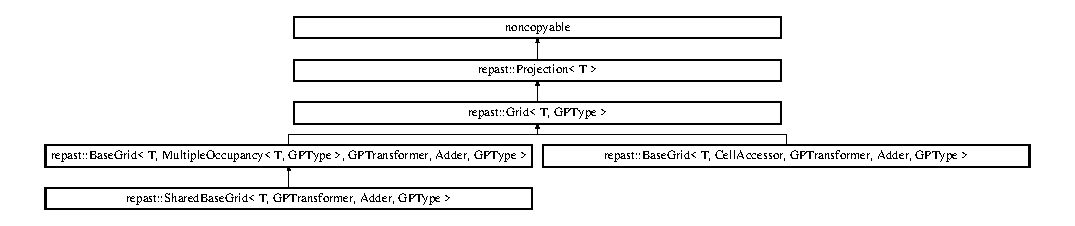
\includegraphics[height=2.587800cm]{classrepast_1_1_grid}
\end{center}
\end{figure}
\subsection*{Public Member Functions}
\begin{DoxyCompactItemize}
\item 
\hyperlink{classrepast_1_1_grid_a0ee11fc5977ad4951f199cb90338c45f}{Grid} (std\-::string \hyperlink{classrepast_1_1_projection_ab60a0ab4f584685780307d7431b61800}{name})
\begin{DoxyCompactList}\small\item\em Creates a \hyperlink{classrepast_1_1_grid}{Grid} with the specified name. \end{DoxyCompactList}\item 
virtual bool \hyperlink{classrepast_1_1_grid_a022599f875eeb1e72c11766500d8282c}{contains} (const \hyperlink{classrepast_1_1_agent_id}{Agent\-Id} \&id)=0
\begin{DoxyCompactList}\small\item\em Gets whether or not this grid contains the agent with the specified id. \end{DoxyCompactList}\item 
virtual bool \hyperlink{classrepast_1_1_grid_ae5bf061d62f1998e0c75bf3967ac63d3}{move\-To} (const \hyperlink{classrepast_1_1_agent_id}{Agent\-Id} \&id, const \hyperlink{classrepast_1_1_point}{Point}$<$ G\-P\-Type $>$ \&pt)=0
\begin{DoxyCompactList}\small\item\em Moves the specified agent to the specified point. \end{DoxyCompactList}\item 
virtual std\-::pair$<$ bool, \hyperlink{classrepast_1_1_point}{Point}\\*
$<$ G\-P\-Type $>$ $>$ \hyperlink{classrepast_1_1_grid_adea1658b984c21ae95bd8f25ecb609b6}{move\-By\-Vector} (const T $\ast$agent, double distance, const std\-::vector$<$ double $>$ \&angles\-In\-Radians)=0
\begin{DoxyCompactList}\small\item\em Moves the specifed object the specified distance from its current position along the specified angle. \end{DoxyCompactList}\item 
virtual std\-::pair$<$ bool, \hyperlink{classrepast_1_1_point}{Point}\\*
$<$ G\-P\-Type $>$ $>$ \hyperlink{classrepast_1_1_grid_a20efd6bdadf8dac405542de7e33f6b9e}{move\-By\-Displacement} (const T $\ast$agent, const std\-::vector$<$ G\-P\-Type $>$ \&displacement)=0
\begin{DoxyCompactList}\small\item\em Moves the specified object from its current location by the specified amount. \end{DoxyCompactList}\item 
virtual const \hyperlink{classrepast_1_1_grid_dimensions}{Grid\-Dimensions} \hyperlink{classrepast_1_1_grid_ac6a979a6491565212ae44b8bfbbc9393}{dimensions} () const =0
\begin{DoxyCompactList}\small\item\em Gets the dimensions of this \hyperlink{classrepast_1_1_grid}{Grid}. \end{DoxyCompactList}\item 
virtual T $\ast$ \hyperlink{classrepast_1_1_grid_a8b77b072353aed6f06b6d02e21ee9879}{get\-Object\-At} (const \hyperlink{classrepast_1_1_point}{Point}$<$ G\-P\-Type $>$ \&pt) const =0
\begin{DoxyCompactList}\small\item\em Gets the first object found at the specified point, or N\-U\-L\-L if there is no such object. \end{DoxyCompactList}\item 
virtual void \hyperlink{classrepast_1_1_grid_aaa3a1fd92707079f7dd4805e36ca83ff}{get\-Objects\-At} (const \hyperlink{classrepast_1_1_point}{Point}$<$ G\-P\-Type $>$ \&pt, std\-::vector$<$ T $\ast$ $>$ \&out) const =0
\begin{DoxyCompactList}\small\item\em Gets all the objects found at the specified point. \end{DoxyCompactList}\item 
virtual bool \hyperlink{classrepast_1_1_grid_a159a33da91ef58dbd8ca88829d82ca36}{get\-Location} (const T $\ast$agent, std\-::vector$<$ G\-P\-Type $>$ \&out) const =0
\begin{DoxyCompactList}\small\item\em Gets the location of this agent and puts it in the specified vector. \end{DoxyCompactList}\item 
virtual bool \hyperlink{classrepast_1_1_grid_a6fef590f66b69e4a06207df59d1b2737}{get\-Location} (const \hyperlink{classrepast_1_1_agent_id}{Agent\-Id} \&id, std\-::vector$<$ G\-P\-Type $>$ \&out) const =0
\begin{DoxyCompactList}\small\item\em Gets the location of this agent and puts it in the specified vectors. \end{DoxyCompactList}\item 
virtual void \hyperlink{classrepast_1_1_grid_a23236c2387ba343121dbf71901dbb341}{get\-Displacement} (const \hyperlink{classrepast_1_1_point}{Point}$<$ G\-P\-Type $>$ \&pt1, const \hyperlink{classrepast_1_1_point}{Point}$<$ G\-P\-Type $>$ \&pt2, std\-::vector$<$ G\-P\-Type $>$ \&out) const =0
\begin{DoxyCompactList}\small\item\em Gets vector difference between point 1 and point 2, putting the result in out. \end{DoxyCompactList}\item 
virtual double \hyperlink{classrepast_1_1_grid_a27213b5f9decf10e1c99a5a7b4ae387a}{get\-Distance} (const \hyperlink{classrepast_1_1_point}{Point}$<$ G\-P\-Type $>$ \&pt1, const \hyperlink{classrepast_1_1_point}{Point}$<$ G\-P\-Type $>$ \&pt2) const =0
\begin{DoxyCompactList}\small\item\em Gets the distance between the two grid points. \end{DoxyCompactList}\item 
virtual double \hyperlink{classrepast_1_1_grid_a456d00d28995a48b41b8f6c84817879e}{get\-Distance\-Sq} (const \hyperlink{classrepast_1_1_point}{Point}$<$ G\-P\-Type $>$ \&pt1, const \hyperlink{classrepast_1_1_point}{Point}$<$ G\-P\-Type $>$ \&pt2) const =0
\begin{DoxyCompactList}\small\item\em Gets the square of the distance between the two grid points. \end{DoxyCompactList}\item 
virtual void \hyperlink{classrepast_1_1_grid_a5aa30c315b9a32830b804d2e49af14d0}{translate} (const \hyperlink{classrepast_1_1_point}{Point}$<$ G\-P\-Type $>$ \&location, const \hyperlink{classrepast_1_1_point}{Point}$<$ G\-P\-Type $>$ \&displacement, std\-::vector$<$ G\-P\-Type $>$ \&out) const =0
\begin{DoxyCompactList}\small\item\em Translates the specified location by the specified displacement put the result in out. \end{DoxyCompactList}\item 
virtual void \hyperlink{classrepast_1_1_grid_a001bf75cd2e436112555a5f992d1d372}{transform} (const std\-::vector$<$ G\-P\-Type $>$ \&location, std\-::vector$<$ G\-P\-Type $>$ \&out) const =0
\begin{DoxyCompactList}\small\item\em Transforms the specified location using the properties (e.\-g. \end{DoxyCompactList}\item 
virtual bool \hyperlink{classrepast_1_1_grid_a81e7eb612dabbf2fb4b3f1190cd92f88}{is\-Periodic} () const =0
\begin{DoxyCompactList}\small\item\em Gets whether or not this grid is periodic (i.\-e. \end{DoxyCompactList}\item 
\hypertarget{classrepast_1_1_grid_a768c6b3b623a0b06e96321738af2da41}{virtual \hyperlink{classrepast_1_1_projection_info_packet}{Projection\-Info\-Packet} $\ast$ {\bfseries get\-Projection\-Info} (\hyperlink{classrepast_1_1_agent_id}{Agent\-Id} id, bool secondary\-Info=false, std\-::set$<$ \hyperlink{classrepast_1_1_agent_id}{Agent\-Id} $>$ $\ast$secondary\-Ids=0, int dest\-Proc=-\/1)=0}\label{classrepast_1_1_grid_a768c6b3b623a0b06e96321738af2da41}

\item 
\hypertarget{classrepast_1_1_grid_a69f9208e8224c3a63a41c935906ffe6b}{virtual void {\bfseries update\-Projection\-Info} (\hyperlink{classrepast_1_1_projection_info_packet}{Projection\-Info\-Packet} $\ast$pip, \hyperlink{classrepast_1_1_context}{Context}$<$ T $>$ $\ast$context)=0}\label{classrepast_1_1_grid_a69f9208e8224c3a63a41c935906ffe6b}

\item 
virtual void \hyperlink{classrepast_1_1_grid_ab1ff08ad641de4f74eab53e30ad14eb6}{get\-Required\-Agents} (std\-::set$<$ \hyperlink{classrepast_1_1_agent_id}{Agent\-Id} $>$ \&agents\-To\-Test, std\-::set$<$ \hyperlink{classrepast_1_1_agent_id}{Agent\-Id} $>$ \&agents\-Required, R\-A\-D\-I\-U\-S radius=\hyperlink{classrepast_1_1_projection}{Projection}$<$ T $>$\-::P\-R\-I\-M\-A\-R\-Y)
\begin{DoxyCompactList}\small\item\em Given a set of agents to test, gets the subset that must be kept in order to fulfill the projection's 'contract' to the specified radius. \end{DoxyCompactList}\item 
virtual void \hyperlink{classrepast_1_1_grid_aa83b294fc8765e2f8ee44d8238855460}{get\-Agents\-To\-Push} (std\-::set$<$ \hyperlink{classrepast_1_1_agent_id}{Agent\-Id} $>$ \&agents\-To\-Test, std\-::map$<$ int, std\-::set$<$ \hyperlink{classrepast_1_1_agent_id}{Agent\-Id} $>$ $>$ \&agents\-To\-Push)=0
\begin{DoxyCompactList}\small\item\em Given a set of agents, gets the agents that this projection implementation must 'push' to other processes. \end{DoxyCompactList}\item 
virtual bool \hyperlink{classrepast_1_1_grid_aa46a5e7692430604bb3b04bbb9e2ff50}{keeps\-Agents\-On\-Sync\-Proj} ()
\begin{DoxyCompactList}\small\item\em Should return true if the \hyperlink{classrepast_1_1_projection}{Projection} implemented can 'keep' some (non-\/local) agents during a projection information synchronization operation. \end{DoxyCompactList}\item 
virtual bool \hyperlink{classrepast_1_1_grid_ae3b7e2de573a9212a58a527a9ab519b8}{sends\-Secondary\-Agents\-On\-Status\-Exchange} ()
\begin{DoxyCompactList}\small\item\em Should return true if the \hyperlink{classrepast_1_1_projection}{Projection} implemented will send secondary agents during a status exchange. \end{DoxyCompactList}\item 
virtual void \hyperlink{classrepast_1_1_grid_a57b4449e602392119eb4db3e0011de05}{get\-Info\-Exchange\-Partners} (std\-::set$<$ int $>$ \&ps\-To\-Send\-To, std\-::set$<$ int $>$ \&ps\-To\-Receive\-From)=0
\begin{DoxyCompactList}\small\item\em Gets the set of processes with which this \hyperlink{classrepast_1_1_projection}{Projection} exchanges projection info. \end{DoxyCompactList}\item 
virtual void \hyperlink{classrepast_1_1_grid_a748354698308fe0d0c0fe33a657109d1}{get\-Agent\-Status\-Exchange\-Partners} (std\-::set$<$ int $>$ \&ps\-To\-Send\-To, std\-::set$<$ int $>$ \&ps\-To\-Receive\-From)=0
\begin{DoxyCompactList}\small\item\em Gets the set of processes with which this \hyperlink{classrepast_1_1_projection}{Projection} exchanges agent status info-\/ that is, the set of processes from which agents can move to this one or to which they can move when moving from this one. \end{DoxyCompactList}\item 
\hypertarget{classrepast_1_1_grid_ae4b6d41862836606e0393df7558e4d20}{virtual void {\bfseries clean\-Projection\-Info} (std\-::set$<$ \hyperlink{classrepast_1_1_agent_id}{Agent\-Id} $>$ \&agents\-To\-Keep)}\label{classrepast_1_1_grid_ae4b6d41862836606e0393df7558e4d20}

\end{DoxyCompactItemize}
\subsection*{Additional Inherited Members}


\subsection{Detailed Description}
\subsubsection*{template$<$typename T, typename G\-P\-Type$>$class repast\-::\-Grid$<$ T, G\-P\-Type $>$}

Abstract interface for Grids and Continuous\-Spaces. 


\begin{DoxyTemplParams}{Template Parameters}
{\em T} & the type of objects this \hyperlink{classrepast_1_1_grid}{Grid} contains \\
\hline
{\em G\-P\-Type} & the coordinate type of the grid point locations. This must be an int or a double. \\
\hline
\end{DoxyTemplParams}


\subsection{Constructor \& Destructor Documentation}
\hypertarget{classrepast_1_1_grid_a0ee11fc5977ad4951f199cb90338c45f}{\index{repast\-::\-Grid@{repast\-::\-Grid}!Grid@{Grid}}
\index{Grid@{Grid}!repast::Grid@{repast\-::\-Grid}}
\subsubsection[{Grid}]{\setlength{\rightskip}{0pt plus 5cm}template$<$typename T, typename G\-P\-Type$>$ {\bf repast\-::\-Grid}$<$ T, G\-P\-Type $>$\-::{\bf Grid} (
\begin{DoxyParamCaption}
\item[{std\-::string}]{name}
\end{DoxyParamCaption}
)\hspace{0.3cm}{\ttfamily [inline]}}}\label{classrepast_1_1_grid_a0ee11fc5977ad4951f199cb90338c45f}


Creates a \hyperlink{classrepast_1_1_grid}{Grid} with the specified name. 


\begin{DoxyParams}{Parameters}
{\em name} & the name of the \hyperlink{classrepast_1_1_grid}{Grid}. This should be unique among Projections. \\
\hline
\end{DoxyParams}


\subsection{Member Function Documentation}
\hypertarget{classrepast_1_1_grid_a022599f875eeb1e72c11766500d8282c}{\index{repast\-::\-Grid@{repast\-::\-Grid}!contains@{contains}}
\index{contains@{contains}!repast::Grid@{repast\-::\-Grid}}
\subsubsection[{contains}]{\setlength{\rightskip}{0pt plus 5cm}template$<$typename T, typename G\-P\-Type$>$ virtual bool {\bf repast\-::\-Grid}$<$ T, G\-P\-Type $>$\-::contains (
\begin{DoxyParamCaption}
\item[{const {\bf Agent\-Id} \&}]{id}
\end{DoxyParamCaption}
)\hspace{0.3cm}{\ttfamily [pure virtual]}}}\label{classrepast_1_1_grid_a022599f875eeb1e72c11766500d8282c}


Gets whether or not this grid contains the agent with the specified id. 


\begin{DoxyParams}{Parameters}
{\em id} & the id of the agent to check\\
\hline
\end{DoxyParams}
\begin{DoxyReturn}{Returns}
true if the grid contains the agent, otherwise false. 
\end{DoxyReturn}


Implemented in \hyperlink{classrepast_1_1_base_grid_a648fcba07fdc15b4072b5807b4f1b6b0}{repast\-::\-Base\-Grid$<$ T, Cell\-Accessor, G\-P\-Transformer, Adder, G\-P\-Type $>$}, \hyperlink{classrepast_1_1_base_grid_a648fcba07fdc15b4072b5807b4f1b6b0}{repast\-::\-Base\-Grid$<$ T, Multiple\-Occupancy$<$ T, double $>$, G\-P\-Transformer, Adder, double $>$}, \hyperlink{classrepast_1_1_base_grid_a648fcba07fdc15b4072b5807b4f1b6b0}{repast\-::\-Base\-Grid$<$ T, Multiple\-Occupancy$<$ T, G\-P\-Type $>$, G\-P\-Transformer, Adder, G\-P\-Type $>$}, and \hyperlink{classrepast_1_1_base_grid_a648fcba07fdc15b4072b5807b4f1b6b0}{repast\-::\-Base\-Grid$<$ T, Multiple\-Occupancy$<$ T, int $>$, G\-P\-Transformer, Adder, int $>$}.

\hypertarget{classrepast_1_1_grid_ac6a979a6491565212ae44b8bfbbc9393}{\index{repast\-::\-Grid@{repast\-::\-Grid}!dimensions@{dimensions}}
\index{dimensions@{dimensions}!repast::Grid@{repast\-::\-Grid}}
\subsubsection[{dimensions}]{\setlength{\rightskip}{0pt plus 5cm}template$<$typename T, typename G\-P\-Type$>$ virtual const {\bf Grid\-Dimensions} {\bf repast\-::\-Grid}$<$ T, G\-P\-Type $>$\-::dimensions (
\begin{DoxyParamCaption}
{}
\end{DoxyParamCaption}
) const\hspace{0.3cm}{\ttfamily [pure virtual]}}}\label{classrepast_1_1_grid_ac6a979a6491565212ae44b8bfbbc9393}


Gets the dimensions of this \hyperlink{classrepast_1_1_grid}{Grid}. 

\begin{DoxyReturn}{Returns}
the dimensions of this \hyperlink{classrepast_1_1_grid}{Grid}. 
\end{DoxyReturn}


Implemented in \hyperlink{classrepast_1_1_shared_base_grid_a9ec19652232000368ec1fe98ff47e121}{repast\-::\-Shared\-Base\-Grid$<$ T, G\-P\-Transformer, Adder, G\-P\-Type $>$}, \hyperlink{classrepast_1_1_shared_base_grid_a9ec19652232000368ec1fe98ff47e121}{repast\-::\-Shared\-Base\-Grid$<$ T, G\-P\-Transformer, Adder, int $>$}, \hyperlink{classrepast_1_1_shared_base_grid_a9ec19652232000368ec1fe98ff47e121}{repast\-::\-Shared\-Base\-Grid$<$ T, G\-P\-Transformer, Adder, double $>$}, \hyperlink{classrepast_1_1_base_grid_a5f8a2fc16b8aeba026a58fcb374cf05c}{repast\-::\-Base\-Grid$<$ T, Cell\-Accessor, G\-P\-Transformer, Adder, G\-P\-Type $>$}, \hyperlink{classrepast_1_1_base_grid_a5f8a2fc16b8aeba026a58fcb374cf05c}{repast\-::\-Base\-Grid$<$ T, Multiple\-Occupancy$<$ T, double $>$, G\-P\-Transformer, Adder, double $>$}, \hyperlink{classrepast_1_1_base_grid_a5f8a2fc16b8aeba026a58fcb374cf05c}{repast\-::\-Base\-Grid$<$ T, Multiple\-Occupancy$<$ T, G\-P\-Type $>$, G\-P\-Transformer, Adder, G\-P\-Type $>$}, and \hyperlink{classrepast_1_1_base_grid_a5f8a2fc16b8aeba026a58fcb374cf05c}{repast\-::\-Base\-Grid$<$ T, Multiple\-Occupancy$<$ T, int $>$, G\-P\-Transformer, Adder, int $>$}.

\hypertarget{classrepast_1_1_grid_a748354698308fe0d0c0fe33a657109d1}{\index{repast\-::\-Grid@{repast\-::\-Grid}!get\-Agent\-Status\-Exchange\-Partners@{get\-Agent\-Status\-Exchange\-Partners}}
\index{get\-Agent\-Status\-Exchange\-Partners@{get\-Agent\-Status\-Exchange\-Partners}!repast::Grid@{repast\-::\-Grid}}
\subsubsection[{get\-Agent\-Status\-Exchange\-Partners}]{\setlength{\rightskip}{0pt plus 5cm}template$<$typename T, typename G\-P\-Type$>$ virtual void {\bf repast\-::\-Grid}$<$ T, G\-P\-Type $>$\-::get\-Agent\-Status\-Exchange\-Partners (
\begin{DoxyParamCaption}
\item[{std\-::set$<$ int $>$ \&}]{ps\-To\-Send\-To, }
\item[{std\-::set$<$ int $>$ \&}]{ps\-To\-Receive\-From}
\end{DoxyParamCaption}
)\hspace{0.3cm}{\ttfamily [pure virtual]}}}\label{classrepast_1_1_grid_a748354698308fe0d0c0fe33a657109d1}


Gets the set of processes with which this \hyperlink{classrepast_1_1_projection}{Projection} exchanges agent status info-\/ that is, the set of processes from which agents can move to this one or to which they can move when moving from this one. 

In the most general case this will be all other processors. However, simulations where agents move in spaces will usually exchange agents only with a small subset of 'neighbor' processes, which is knowable in advance and constant. To accommodate the general case, the algorithm for exchanging information must poll all other processes to see which are sending to this one; if this is known in advance, this additional (expensive) step can be skipped. 

Implements \hyperlink{classrepast_1_1_projection_ad2d104bb6119d0911053d450932855d5}{repast\-::\-Projection$<$ T $>$}.



Implemented in \hyperlink{classrepast_1_1_shared_base_grid_a0388d98240eb59548058d3c45da702d7}{repast\-::\-Shared\-Base\-Grid$<$ T, G\-P\-Transformer, Adder, G\-P\-Type $>$}, \hyperlink{classrepast_1_1_shared_base_grid_a0388d98240eb59548058d3c45da702d7}{repast\-::\-Shared\-Base\-Grid$<$ T, G\-P\-Transformer, Adder, int $>$}, and \hyperlink{classrepast_1_1_shared_base_grid_a0388d98240eb59548058d3c45da702d7}{repast\-::\-Shared\-Base\-Grid$<$ T, G\-P\-Transformer, Adder, double $>$}.

\hypertarget{classrepast_1_1_grid_aa83b294fc8765e2f8ee44d8238855460}{\index{repast\-::\-Grid@{repast\-::\-Grid}!get\-Agents\-To\-Push@{get\-Agents\-To\-Push}}
\index{get\-Agents\-To\-Push@{get\-Agents\-To\-Push}!repast::Grid@{repast\-::\-Grid}}
\subsubsection[{get\-Agents\-To\-Push}]{\setlength{\rightskip}{0pt plus 5cm}template$<$typename T, typename G\-P\-Type$>$ virtual void {\bf repast\-::\-Grid}$<$ T, G\-P\-Type $>$\-::get\-Agents\-To\-Push (
\begin{DoxyParamCaption}
\item[{std\-::set$<$ {\bf Agent\-Id} $>$ \&}]{agents\-To\-Test, }
\item[{std\-::map$<$ int, std\-::set$<$ {\bf Agent\-Id} $>$ $>$ \&}]{agents\-To\-Push}
\end{DoxyParamCaption}
)\hspace{0.3cm}{\ttfamily [pure virtual]}}}\label{classrepast_1_1_grid_aa83b294fc8765e2f8ee44d8238855460}


Given a set of agents, gets the agents that this projection implementation must 'push' to other processes. 

Generally spaces must push agents that are in 'buffer zones' and graphs must push local agents that are vertices to master edges where the other vertex is non-\/ local. The results are returned per-\/process in the agents\-To\-Push map. 

Implements \hyperlink{classrepast_1_1_projection_ae1877809facd80a5e25d95e3dc5c35f4}{repast\-::\-Projection$<$ T $>$}.



Implemented in \hyperlink{classrepast_1_1_shared_base_grid_ab1486e7698288efc1218653d4e5e1e15}{repast\-::\-Shared\-Base\-Grid$<$ T, G\-P\-Transformer, Adder, G\-P\-Type $>$}, \hyperlink{classrepast_1_1_shared_base_grid_ab1486e7698288efc1218653d4e5e1e15}{repast\-::\-Shared\-Base\-Grid$<$ T, G\-P\-Transformer, Adder, int $>$}, \hyperlink{classrepast_1_1_shared_base_grid_ab1486e7698288efc1218653d4e5e1e15}{repast\-::\-Shared\-Base\-Grid$<$ T, G\-P\-Transformer, Adder, double $>$}, \hyperlink{classrepast_1_1_base_grid_a8f718ade5af8285f71151eea824ce3cd}{repast\-::\-Base\-Grid$<$ T, Cell\-Accessor, G\-P\-Transformer, Adder, G\-P\-Type $>$}, \hyperlink{classrepast_1_1_base_grid_a8f718ade5af8285f71151eea824ce3cd}{repast\-::\-Base\-Grid$<$ T, Multiple\-Occupancy$<$ T, double $>$, G\-P\-Transformer, Adder, double $>$}, \hyperlink{classrepast_1_1_base_grid_a8f718ade5af8285f71151eea824ce3cd}{repast\-::\-Base\-Grid$<$ T, Multiple\-Occupancy$<$ T, G\-P\-Type $>$, G\-P\-Transformer, Adder, G\-P\-Type $>$}, \hyperlink{classrepast_1_1_base_grid_a8f718ade5af8285f71151eea824ce3cd}{repast\-::\-Base\-Grid$<$ T, Multiple\-Occupancy$<$ T, int $>$, G\-P\-Transformer, Adder, int $>$}, and \hyperlink{classrepast_1_1_shared_discrete_space_a1f690e82e6b7ea6a279db020e12b4d21}{repast\-::\-Shared\-Discrete\-Space$<$ T, G\-P\-Transformer, Adder $>$}.

\hypertarget{classrepast_1_1_grid_a23236c2387ba343121dbf71901dbb341}{\index{repast\-::\-Grid@{repast\-::\-Grid}!get\-Displacement@{get\-Displacement}}
\index{get\-Displacement@{get\-Displacement}!repast::Grid@{repast\-::\-Grid}}
\subsubsection[{get\-Displacement}]{\setlength{\rightskip}{0pt plus 5cm}template$<$typename T, typename G\-P\-Type$>$ virtual void {\bf repast\-::\-Grid}$<$ T, G\-P\-Type $>$\-::get\-Displacement (
\begin{DoxyParamCaption}
\item[{const {\bf Point}$<$ G\-P\-Type $>$ \&}]{pt1, }
\item[{const {\bf Point}$<$ G\-P\-Type $>$ \&}]{pt2, }
\item[{std\-::vector$<$ G\-P\-Type $>$ \&}]{out}
\end{DoxyParamCaption}
) const\hspace{0.3cm}{\ttfamily [pure virtual]}}}\label{classrepast_1_1_grid_a23236c2387ba343121dbf71901dbb341}


Gets vector difference between point 1 and point 2, putting the result in out. 


\begin{DoxyParams}[1]{Parameters}
 & {\em p1} & the first point \\
\hline
 & {\em p2} & the second point \\
\hline
\mbox{\tt out}  & {\em the} & vector where the difference will be put \\
\hline
\end{DoxyParams}


Implemented in \hyperlink{classrepast_1_1_base_grid_a8c3b8755d2fc2bf75163a0fc76ce1d4a}{repast\-::\-Base\-Grid$<$ T, Cell\-Accessor, G\-P\-Transformer, Adder, G\-P\-Type $>$}, \hyperlink{classrepast_1_1_base_grid_a8c3b8755d2fc2bf75163a0fc76ce1d4a}{repast\-::\-Base\-Grid$<$ T, Multiple\-Occupancy$<$ T, double $>$, G\-P\-Transformer, Adder, double $>$}, \hyperlink{classrepast_1_1_base_grid_a8c3b8755d2fc2bf75163a0fc76ce1d4a}{repast\-::\-Base\-Grid$<$ T, Multiple\-Occupancy$<$ T, G\-P\-Type $>$, G\-P\-Transformer, Adder, G\-P\-Type $>$}, and \hyperlink{classrepast_1_1_base_grid_a8c3b8755d2fc2bf75163a0fc76ce1d4a}{repast\-::\-Base\-Grid$<$ T, Multiple\-Occupancy$<$ T, int $>$, G\-P\-Transformer, Adder, int $>$}.

\hypertarget{classrepast_1_1_grid_a27213b5f9decf10e1c99a5a7b4ae387a}{\index{repast\-::\-Grid@{repast\-::\-Grid}!get\-Distance@{get\-Distance}}
\index{get\-Distance@{get\-Distance}!repast::Grid@{repast\-::\-Grid}}
\subsubsection[{get\-Distance}]{\setlength{\rightskip}{0pt plus 5cm}template$<$typename T, typename G\-P\-Type$>$ virtual double {\bf repast\-::\-Grid}$<$ T, G\-P\-Type $>$\-::get\-Distance (
\begin{DoxyParamCaption}
\item[{const {\bf Point}$<$ G\-P\-Type $>$ \&}]{pt1, }
\item[{const {\bf Point}$<$ G\-P\-Type $>$ \&}]{pt2}
\end{DoxyParamCaption}
) const\hspace{0.3cm}{\ttfamily [pure virtual]}}}\label{classrepast_1_1_grid_a27213b5f9decf10e1c99a5a7b4ae387a}


Gets the distance between the two grid points. 


\begin{DoxyParams}{Parameters}
{\em p1} & the first point \\
\hline
{\em p2} & the second point\\
\hline
\end{DoxyParams}
\begin{DoxyReturn}{Returns}
the distance between pt1 and pt2. 
\end{DoxyReturn}


Implemented in \hyperlink{classrepast_1_1_base_grid_a124b5f53a5e96e9ed8e59534e9417f42}{repast\-::\-Base\-Grid$<$ T, Cell\-Accessor, G\-P\-Transformer, Adder, G\-P\-Type $>$}, \hyperlink{classrepast_1_1_base_grid_a124b5f53a5e96e9ed8e59534e9417f42}{repast\-::\-Base\-Grid$<$ T, Multiple\-Occupancy$<$ T, double $>$, G\-P\-Transformer, Adder, double $>$}, \hyperlink{classrepast_1_1_base_grid_a124b5f53a5e96e9ed8e59534e9417f42}{repast\-::\-Base\-Grid$<$ T, Multiple\-Occupancy$<$ T, G\-P\-Type $>$, G\-P\-Transformer, Adder, G\-P\-Type $>$}, and \hyperlink{classrepast_1_1_base_grid_a124b5f53a5e96e9ed8e59534e9417f42}{repast\-::\-Base\-Grid$<$ T, Multiple\-Occupancy$<$ T, int $>$, G\-P\-Transformer, Adder, int $>$}.

\hypertarget{classrepast_1_1_grid_a456d00d28995a48b41b8f6c84817879e}{\index{repast\-::\-Grid@{repast\-::\-Grid}!get\-Distance\-Sq@{get\-Distance\-Sq}}
\index{get\-Distance\-Sq@{get\-Distance\-Sq}!repast::Grid@{repast\-::\-Grid}}
\subsubsection[{get\-Distance\-Sq}]{\setlength{\rightskip}{0pt plus 5cm}template$<$typename T, typename G\-P\-Type$>$ virtual double {\bf repast\-::\-Grid}$<$ T, G\-P\-Type $>$\-::get\-Distance\-Sq (
\begin{DoxyParamCaption}
\item[{const {\bf Point}$<$ G\-P\-Type $>$ \&}]{pt1, }
\item[{const {\bf Point}$<$ G\-P\-Type $>$ \&}]{pt2}
\end{DoxyParamCaption}
) const\hspace{0.3cm}{\ttfamily [pure virtual]}}}\label{classrepast_1_1_grid_a456d00d28995a48b41b8f6c84817879e}


Gets the square of the distance between the two grid points. 


\begin{DoxyParams}{Parameters}
{\em p1} & the first point \\
\hline
{\em p2} & the second point\\
\hline
\end{DoxyParams}
\begin{DoxyReturn}{Returns}
the square of the distance between pt1 and pt2. 
\end{DoxyReturn}


Implemented in \hyperlink{classrepast_1_1_base_grid_a8075dd20e6d559d453a530943ab9d387}{repast\-::\-Base\-Grid$<$ T, Cell\-Accessor, G\-P\-Transformer, Adder, G\-P\-Type $>$}, \hyperlink{classrepast_1_1_base_grid_a8075dd20e6d559d453a530943ab9d387}{repast\-::\-Base\-Grid$<$ T, Multiple\-Occupancy$<$ T, double $>$, G\-P\-Transformer, Adder, double $>$}, \hyperlink{classrepast_1_1_base_grid_a8075dd20e6d559d453a530943ab9d387}{repast\-::\-Base\-Grid$<$ T, Multiple\-Occupancy$<$ T, G\-P\-Type $>$, G\-P\-Transformer, Adder, G\-P\-Type $>$}, and \hyperlink{classrepast_1_1_base_grid_a8075dd20e6d559d453a530943ab9d387}{repast\-::\-Base\-Grid$<$ T, Multiple\-Occupancy$<$ T, int $>$, G\-P\-Transformer, Adder, int $>$}.

\hypertarget{classrepast_1_1_grid_a57b4449e602392119eb4db3e0011de05}{\index{repast\-::\-Grid@{repast\-::\-Grid}!get\-Info\-Exchange\-Partners@{get\-Info\-Exchange\-Partners}}
\index{get\-Info\-Exchange\-Partners@{get\-Info\-Exchange\-Partners}!repast::Grid@{repast\-::\-Grid}}
\subsubsection[{get\-Info\-Exchange\-Partners}]{\setlength{\rightskip}{0pt plus 5cm}template$<$typename T, typename G\-P\-Type$>$ virtual void {\bf repast\-::\-Grid}$<$ T, G\-P\-Type $>$\-::get\-Info\-Exchange\-Partners (
\begin{DoxyParamCaption}
\item[{std\-::set$<$ int $>$ \&}]{ps\-To\-Send\-To, }
\item[{std\-::set$<$ int $>$ \&}]{ps\-To\-Receive\-From}
\end{DoxyParamCaption}
)\hspace{0.3cm}{\ttfamily [pure virtual]}}}\label{classrepast_1_1_grid_a57b4449e602392119eb4db3e0011de05}


Gets the set of processes with which this \hyperlink{classrepast_1_1_projection}{Projection} exchanges projection info. 

In the most general case this will be all other processors; this is the case for graphs, where agent connections can be arbitrary. However, spaces usually exchange information only with a small subset of 'neighbor' processes, which is knowable in advance and constant. To accommodate the general case, the algorithm for exchanging information must poll all other processes to see which are sending to this one; if this is known in advance, this additional (expensive) step can be skipped. 

Implements \hyperlink{classrepast_1_1_projection_afdc13fccb129094bfd67b3446873933d}{repast\-::\-Projection$<$ T $>$}.



Implemented in \hyperlink{classrepast_1_1_shared_base_grid_af4323686714c4f6216125db5609c3184}{repast\-::\-Shared\-Base\-Grid$<$ T, G\-P\-Transformer, Adder, G\-P\-Type $>$}, \hyperlink{classrepast_1_1_shared_base_grid_af4323686714c4f6216125db5609c3184}{repast\-::\-Shared\-Base\-Grid$<$ T, G\-P\-Transformer, Adder, int $>$}, and \hyperlink{classrepast_1_1_shared_base_grid_af4323686714c4f6216125db5609c3184}{repast\-::\-Shared\-Base\-Grid$<$ T, G\-P\-Transformer, Adder, double $>$}.

\hypertarget{classrepast_1_1_grid_a159a33da91ef58dbd8ca88829d82ca36}{\index{repast\-::\-Grid@{repast\-::\-Grid}!get\-Location@{get\-Location}}
\index{get\-Location@{get\-Location}!repast::Grid@{repast\-::\-Grid}}
\subsubsection[{get\-Location}]{\setlength{\rightskip}{0pt plus 5cm}template$<$typename T, typename G\-P\-Type$>$ virtual bool {\bf repast\-::\-Grid}$<$ T, G\-P\-Type $>$\-::get\-Location (
\begin{DoxyParamCaption}
\item[{const T $\ast$}]{agent, }
\item[{std\-::vector$<$ G\-P\-Type $>$ \&}]{out}
\end{DoxyParamCaption}
) const\hspace{0.3cm}{\ttfamily [pure virtual]}}}\label{classrepast_1_1_grid_a159a33da91ef58dbd8ca88829d82ca36}


Gets the location of this agent and puts it in the specified vector. 

The x coordinate will be the first value, the y the second and so on.


\begin{DoxyParams}[1]{Parameters}
 & {\em agent} & the agent whose location we want to get \\
\hline
\mbox{\tt out}  & {\em the} & vector where the agents location will be put\\
\hline
\end{DoxyParams}
\begin{DoxyReturn}{Returns}
true if the location was successfully found, otherwise false. 
\end{DoxyReturn}


Implemented in \hyperlink{classrepast_1_1_base_grid_a9ef8aae56bb771fa152b10408d718f6e}{repast\-::\-Base\-Grid$<$ T, Cell\-Accessor, G\-P\-Transformer, Adder, G\-P\-Type $>$}, \hyperlink{classrepast_1_1_base_grid_a9ef8aae56bb771fa152b10408d718f6e}{repast\-::\-Base\-Grid$<$ T, Multiple\-Occupancy$<$ T, double $>$, G\-P\-Transformer, Adder, double $>$}, \hyperlink{classrepast_1_1_base_grid_a9ef8aae56bb771fa152b10408d718f6e}{repast\-::\-Base\-Grid$<$ T, Multiple\-Occupancy$<$ T, G\-P\-Type $>$, G\-P\-Transformer, Adder, G\-P\-Type $>$}, and \hyperlink{classrepast_1_1_base_grid_a9ef8aae56bb771fa152b10408d718f6e}{repast\-::\-Base\-Grid$<$ T, Multiple\-Occupancy$<$ T, int $>$, G\-P\-Transformer, Adder, int $>$}.

\hypertarget{classrepast_1_1_grid_a6fef590f66b69e4a06207df59d1b2737}{\index{repast\-::\-Grid@{repast\-::\-Grid}!get\-Location@{get\-Location}}
\index{get\-Location@{get\-Location}!repast::Grid@{repast\-::\-Grid}}
\subsubsection[{get\-Location}]{\setlength{\rightskip}{0pt plus 5cm}template$<$typename T, typename G\-P\-Type$>$ virtual bool {\bf repast\-::\-Grid}$<$ T, G\-P\-Type $>$\-::get\-Location (
\begin{DoxyParamCaption}
\item[{const {\bf Agent\-Id} \&}]{id, }
\item[{std\-::vector$<$ G\-P\-Type $>$ \&}]{out}
\end{DoxyParamCaption}
) const\hspace{0.3cm}{\ttfamily [pure virtual]}}}\label{classrepast_1_1_grid_a6fef590f66b69e4a06207df59d1b2737}


Gets the location of this agent and puts it in the specified vectors. 

The x coordinate will be the first value, the y the second and so on.


\begin{DoxyParams}[1]{Parameters}
 & {\em id} & the id of the agent whose location we want to get \\
\hline
\mbox{\tt out}  & {\em out} & the agent's location will be put into this vector\\
\hline
\end{DoxyParams}
\begin{DoxyReturn}{Returns}
true if the location was successfully found, otherwise false. 
\end{DoxyReturn}


Implemented in \hyperlink{classrepast_1_1_base_grid_aa18b424b73ff46fde970ad1e1bb3cdc4}{repast\-::\-Base\-Grid$<$ T, Cell\-Accessor, G\-P\-Transformer, Adder, G\-P\-Type $>$}, \hyperlink{classrepast_1_1_base_grid_aa18b424b73ff46fde970ad1e1bb3cdc4}{repast\-::\-Base\-Grid$<$ T, Multiple\-Occupancy$<$ T, double $>$, G\-P\-Transformer, Adder, double $>$}, \hyperlink{classrepast_1_1_base_grid_aa18b424b73ff46fde970ad1e1bb3cdc4}{repast\-::\-Base\-Grid$<$ T, Multiple\-Occupancy$<$ T, G\-P\-Type $>$, G\-P\-Transformer, Adder, G\-P\-Type $>$}, and \hyperlink{classrepast_1_1_base_grid_aa18b424b73ff46fde970ad1e1bb3cdc4}{repast\-::\-Base\-Grid$<$ T, Multiple\-Occupancy$<$ T, int $>$, G\-P\-Transformer, Adder, int $>$}.

\hypertarget{classrepast_1_1_grid_a8b77b072353aed6f06b6d02e21ee9879}{\index{repast\-::\-Grid@{repast\-::\-Grid}!get\-Object\-At@{get\-Object\-At}}
\index{get\-Object\-At@{get\-Object\-At}!repast::Grid@{repast\-::\-Grid}}
\subsubsection[{get\-Object\-At}]{\setlength{\rightskip}{0pt plus 5cm}template$<$typename T, typename G\-P\-Type$>$ virtual T$\ast$ {\bf repast\-::\-Grid}$<$ T, G\-P\-Type $>$\-::get\-Object\-At (
\begin{DoxyParamCaption}
\item[{const {\bf Point}$<$ G\-P\-Type $>$ \&}]{pt}
\end{DoxyParamCaption}
) const\hspace{0.3cm}{\ttfamily [pure virtual]}}}\label{classrepast_1_1_grid_a8b77b072353aed6f06b6d02e21ee9879}


Gets the first object found at the specified point, or N\-U\-L\-L if there is no such object. 

\begin{DoxyReturn}{Returns}
the first object found at the specified point, or N\-U\-L\-L if there is no such object. 
\end{DoxyReturn}


Implemented in \hyperlink{classrepast_1_1_base_grid_a3710f4aca96eeb3a95a44fe80e0c998a}{repast\-::\-Base\-Grid$<$ T, Cell\-Accessor, G\-P\-Transformer, Adder, G\-P\-Type $>$}, \hyperlink{classrepast_1_1_base_grid_a3710f4aca96eeb3a95a44fe80e0c998a}{repast\-::\-Base\-Grid$<$ T, Multiple\-Occupancy$<$ T, double $>$, G\-P\-Transformer, Adder, double $>$}, \hyperlink{classrepast_1_1_base_grid_a3710f4aca96eeb3a95a44fe80e0c998a}{repast\-::\-Base\-Grid$<$ T, Multiple\-Occupancy$<$ T, G\-P\-Type $>$, G\-P\-Transformer, Adder, G\-P\-Type $>$}, and \hyperlink{classrepast_1_1_base_grid_a3710f4aca96eeb3a95a44fe80e0c998a}{repast\-::\-Base\-Grid$<$ T, Multiple\-Occupancy$<$ T, int $>$, G\-P\-Transformer, Adder, int $>$}.

\hypertarget{classrepast_1_1_grid_aaa3a1fd92707079f7dd4805e36ca83ff}{\index{repast\-::\-Grid@{repast\-::\-Grid}!get\-Objects\-At@{get\-Objects\-At}}
\index{get\-Objects\-At@{get\-Objects\-At}!repast::Grid@{repast\-::\-Grid}}
\subsubsection[{get\-Objects\-At}]{\setlength{\rightskip}{0pt plus 5cm}template$<$typename T, typename G\-P\-Type$>$ virtual void {\bf repast\-::\-Grid}$<$ T, G\-P\-Type $>$\-::get\-Objects\-At (
\begin{DoxyParamCaption}
\item[{const {\bf Point}$<$ G\-P\-Type $>$ \&}]{pt, }
\item[{std\-::vector$<$ T $\ast$ $>$ \&}]{out}
\end{DoxyParamCaption}
) const\hspace{0.3cm}{\ttfamily [pure virtual]}}}\label{classrepast_1_1_grid_aaa3a1fd92707079f7dd4805e36ca83ff}


Gets all the objects found at the specified point. 

The found objects will be put into the out parameter.


\begin{DoxyParams}[1]{Parameters}
 & {\em pt} & the point to get all the objects at \\
\hline
\mbox{\tt out}  & {\em out} & the vector into which the found objects will be put \\
\hline
\end{DoxyParams}


Implemented in \hyperlink{classrepast_1_1_base_grid_a21d840f3eb758b8f223ca51bf1996328}{repast\-::\-Base\-Grid$<$ T, Cell\-Accessor, G\-P\-Transformer, Adder, G\-P\-Type $>$}, \hyperlink{classrepast_1_1_base_grid_a21d840f3eb758b8f223ca51bf1996328}{repast\-::\-Base\-Grid$<$ T, Multiple\-Occupancy$<$ T, double $>$, G\-P\-Transformer, Adder, double $>$}, \hyperlink{classrepast_1_1_base_grid_a21d840f3eb758b8f223ca51bf1996328}{repast\-::\-Base\-Grid$<$ T, Multiple\-Occupancy$<$ T, G\-P\-Type $>$, G\-P\-Transformer, Adder, G\-P\-Type $>$}, and \hyperlink{classrepast_1_1_base_grid_a21d840f3eb758b8f223ca51bf1996328}{repast\-::\-Base\-Grid$<$ T, Multiple\-Occupancy$<$ T, int $>$, G\-P\-Transformer, Adder, int $>$}.

\hypertarget{classrepast_1_1_grid_ab1ff08ad641de4f74eab53e30ad14eb6}{\index{repast\-::\-Grid@{repast\-::\-Grid}!get\-Required\-Agents@{get\-Required\-Agents}}
\index{get\-Required\-Agents@{get\-Required\-Agents}!repast::Grid@{repast\-::\-Grid}}
\subsubsection[{get\-Required\-Agents}]{\setlength{\rightskip}{0pt plus 5cm}template$<$typename T, typename G\-P\-Type$>$ virtual void {\bf repast\-::\-Grid}$<$ T, G\-P\-Type $>$\-::get\-Required\-Agents (
\begin{DoxyParamCaption}
\item[{std\-::set$<$ {\bf Agent\-Id} $>$ \&}]{agents\-To\-Test, }
\item[{std\-::set$<$ {\bf Agent\-Id} $>$ \&}]{agents\-Required, }
\item[{R\-A\-D\-I\-U\-S}]{radius = {\ttfamily {\bf Projection}$<$~T~$>$\-:\-:PRIMARY}}
\end{DoxyParamCaption}
)\hspace{0.3cm}{\ttfamily [inline]}, {\ttfamily [virtual]}}}\label{classrepast_1_1_grid_ab1ff08ad641de4f74eab53e30ad14eb6}


Given a set of agents to test, gets the subset that must be kept in order to fulfill the projection's 'contract' to the specified radius. 

Generally spaces do not require any agents, but graphs do-\/ generally the non-\/local ends to master copies of edges. 

Implements \hyperlink{classrepast_1_1_projection_ad13ded8db8e364aa43efde5b35da9a65}{repast\-::\-Projection$<$ T $>$}.

\hypertarget{classrepast_1_1_grid_a81e7eb612dabbf2fb4b3f1190cd92f88}{\index{repast\-::\-Grid@{repast\-::\-Grid}!is\-Periodic@{is\-Periodic}}
\index{is\-Periodic@{is\-Periodic}!repast::Grid@{repast\-::\-Grid}}
\subsubsection[{is\-Periodic}]{\setlength{\rightskip}{0pt plus 5cm}template$<$typename T, typename G\-P\-Type$>$ virtual bool {\bf repast\-::\-Grid}$<$ T, G\-P\-Type $>$\-::is\-Periodic (
\begin{DoxyParamCaption}
{}
\end{DoxyParamCaption}
) const\hspace{0.3cm}{\ttfamily [pure virtual]}}}\label{classrepast_1_1_grid_a81e7eb612dabbf2fb4b3f1190cd92f88}


Gets whether or not this grid is periodic (i.\-e. 

toroidal).

\begin{DoxyReturn}{Returns}
true if this \hyperlink{classrepast_1_1_grid}{Grid} is periodic, otherwise false. 
\end{DoxyReturn}


Implemented in \hyperlink{classrepast_1_1_base_grid_a4dd5ec33acc952ab136f5e2b9886771e}{repast\-::\-Base\-Grid$<$ T, Cell\-Accessor, G\-P\-Transformer, Adder, G\-P\-Type $>$}, \hyperlink{classrepast_1_1_base_grid_a4dd5ec33acc952ab136f5e2b9886771e}{repast\-::\-Base\-Grid$<$ T, Multiple\-Occupancy$<$ T, double $>$, G\-P\-Transformer, Adder, double $>$}, \hyperlink{classrepast_1_1_base_grid_a4dd5ec33acc952ab136f5e2b9886771e}{repast\-::\-Base\-Grid$<$ T, Multiple\-Occupancy$<$ T, G\-P\-Type $>$, G\-P\-Transformer, Adder, G\-P\-Type $>$}, and \hyperlink{classrepast_1_1_base_grid_a4dd5ec33acc952ab136f5e2b9886771e}{repast\-::\-Base\-Grid$<$ T, Multiple\-Occupancy$<$ T, int $>$, G\-P\-Transformer, Adder, int $>$}.

\hypertarget{classrepast_1_1_grid_aa46a5e7692430604bb3b04bbb9e2ff50}{\index{repast\-::\-Grid@{repast\-::\-Grid}!keeps\-Agents\-On\-Sync\-Proj@{keeps\-Agents\-On\-Sync\-Proj}}
\index{keeps\-Agents\-On\-Sync\-Proj@{keeps\-Agents\-On\-Sync\-Proj}!repast::Grid@{repast\-::\-Grid}}
\subsubsection[{keeps\-Agents\-On\-Sync\-Proj}]{\setlength{\rightskip}{0pt plus 5cm}template$<$typename T, typename G\-P\-Type$>$ virtual bool {\bf repast\-::\-Grid}$<$ T, G\-P\-Type $>$\-::keeps\-Agents\-On\-Sync\-Proj (
\begin{DoxyParamCaption}
{}
\end{DoxyParamCaption}
)\hspace{0.3cm}{\ttfamily [inline]}, {\ttfamily [virtual]}}}\label{classrepast_1_1_grid_aa46a5e7692430604bb3b04bbb9e2ff50}


Should return true if the \hyperlink{classrepast_1_1_projection}{Projection} implemented can 'keep' some (non-\/local) agents during a projection information synchronization operation. 

Generally spaces will allow all non-\/local agents to be deleted, but graphs keep the non-\/local agents that participate in Master edges.

It is possible to override these. A graph projection can be created that does not permit non-\/local agents to be 'kept'. This would be an extremely unusual use case, but it is possible.

Note that these are used for optimization. If no projection in a given context keeps any agents, several steps in the synchronization algorithm can be omitted. Of course, omitting these steps when a projection actually retains agents can caused undefined problems.

\begin{DoxyReturn}{Returns}
true if this projection will keep non-\/local agents during a projection information synchronziation event, false if it will not. 
\end{DoxyReturn}


Implements \hyperlink{classrepast_1_1_projection_a1da1dcc47517e3e25be129067b21601f}{repast\-::\-Projection$<$ T $>$}.

\hypertarget{classrepast_1_1_grid_a20efd6bdadf8dac405542de7e33f6b9e}{\index{repast\-::\-Grid@{repast\-::\-Grid}!move\-By\-Displacement@{move\-By\-Displacement}}
\index{move\-By\-Displacement@{move\-By\-Displacement}!repast::Grid@{repast\-::\-Grid}}
\subsubsection[{move\-By\-Displacement}]{\setlength{\rightskip}{0pt plus 5cm}template$<$typename T, typename G\-P\-Type$>$ virtual std\-::pair$<$bool, {\bf Point}$<$G\-P\-Type$>$ $>$ {\bf repast\-::\-Grid}$<$ T, G\-P\-Type $>$\-::move\-By\-Displacement (
\begin{DoxyParamCaption}
\item[{const T $\ast$}]{agent, }
\item[{const std\-::vector$<$ G\-P\-Type $>$ \&}]{displacement}
\end{DoxyParamCaption}
)\hspace{0.3cm}{\ttfamily [pure virtual]}}}\label{classrepast_1_1_grid_a20efd6bdadf8dac405542de7e33f6b9e}


Moves the specified object from its current location by the specified amount. 

For example {\ttfamily move\-By\-Displacement(object, 3, -\/2, 1)} will move the object by 3 along the x-\/axis, -\/2 along the y and 1 along the z. The displacement argument can be less than the number of dimensions in the space in which case the remaining argument will be set to 0. For example, {\ttfamily move\-By\-Displacement(object, 3)} will move the object 3 along the x-\/axis and 0 along the y and z axes, assuming a 3\-D grid.


\begin{DoxyParams}{Parameters}
{\em agent} & the object to move \\
\hline
{\em displacement} & the amount to move the object \\
\hline
\end{DoxyParams}
\begin{DoxyReturn}{Returns}
a pair containing a bool that indicates whether the move was a success or not, and the point where the agent was moved to. 
\end{DoxyReturn}


Implemented in \hyperlink{classrepast_1_1_base_grid_a75758e9f795679c0a9c9b92fbd9413af}{repast\-::\-Base\-Grid$<$ T, Cell\-Accessor, G\-P\-Transformer, Adder, G\-P\-Type $>$}, \hyperlink{classrepast_1_1_base_grid_a75758e9f795679c0a9c9b92fbd9413af}{repast\-::\-Base\-Grid$<$ T, Multiple\-Occupancy$<$ T, double $>$, G\-P\-Transformer, Adder, double $>$}, \hyperlink{classrepast_1_1_base_grid_a75758e9f795679c0a9c9b92fbd9413af}{repast\-::\-Base\-Grid$<$ T, Multiple\-Occupancy$<$ T, G\-P\-Type $>$, G\-P\-Transformer, Adder, G\-P\-Type $>$}, and \hyperlink{classrepast_1_1_base_grid_a75758e9f795679c0a9c9b92fbd9413af}{repast\-::\-Base\-Grid$<$ T, Multiple\-Occupancy$<$ T, int $>$, G\-P\-Transformer, Adder, int $>$}.

\hypertarget{classrepast_1_1_grid_adea1658b984c21ae95bd8f25ecb609b6}{\index{repast\-::\-Grid@{repast\-::\-Grid}!move\-By\-Vector@{move\-By\-Vector}}
\index{move\-By\-Vector@{move\-By\-Vector}!repast::Grid@{repast\-::\-Grid}}
\subsubsection[{move\-By\-Vector}]{\setlength{\rightskip}{0pt plus 5cm}template$<$typename T, typename G\-P\-Type$>$ virtual std\-::pair$<$bool, {\bf Point}$<$G\-P\-Type$>$ $>$ {\bf repast\-::\-Grid}$<$ T, G\-P\-Type $>$\-::move\-By\-Vector (
\begin{DoxyParamCaption}
\item[{const T $\ast$}]{agent, }
\item[{double}]{distance, }
\item[{const std\-::vector$<$ double $>$ \&}]{angles\-In\-Radians}
\end{DoxyParamCaption}
)\hspace{0.3cm}{\ttfamily [pure virtual]}}}\label{classrepast_1_1_grid_adea1658b984c21ae95bd8f25ecb609b6}


Moves the specifed object the specified distance from its current position along the specified angle. 

For example, {\ttfamily move\-By\-Vector(object, 1, Grid.\-N\-O\-R\-T\-H)} will move the object 1 unit \char`\"{}north\char`\"{} up the y-\/axis, assuming a 2\-D grid. Similarly, {\ttfamily grid.\-move\-By\-Vector(object, 2, 0, Math.\-to\-Radians(90), 0)} will rotate 90 degrees around the y-\/axis, thus moving the object 2 units along the z-\/axis. 

{\bfseries  Note that the radians / degrees are incremented in a anti-\/clockwise fashion, such that 0 degrees is \char`\"{}east\char`\"{}, 90 degrees is \char`\"{}north\char`\"{}, 180 is \char`\"{}west\char`\"{} and 270 is \char`\"{}south.\char`\"{}}

{\bfseries 
\begin{DoxyParams}{Parameters}
{\em agent} & the object to move \\
\hline
{\em distance} & the distance to move \\
\hline
{\em angles\-In\-Radians} & the angle to move along in radians. \\
\hline
\end{DoxyParams}
\begin{DoxyReturn}{Returns}
a pair containing a bool that indicates whether the move was a success or not, and the point where the agent was moved to. 
\end{DoxyReturn}
}

Implemented in \hyperlink{classrepast_1_1_base_grid_a14de646e4c01d6bcd0356669a23af43d}{repast\-::\-Base\-Grid$<$ T, Cell\-Accessor, G\-P\-Transformer, Adder, G\-P\-Type $>$}, \hyperlink{classrepast_1_1_base_grid_a14de646e4c01d6bcd0356669a23af43d}{repast\-::\-Base\-Grid$<$ T, Multiple\-Occupancy$<$ T, double $>$, G\-P\-Transformer, Adder, double $>$}, \hyperlink{classrepast_1_1_base_grid_a14de646e4c01d6bcd0356669a23af43d}{repast\-::\-Base\-Grid$<$ T, Multiple\-Occupancy$<$ T, G\-P\-Type $>$, G\-P\-Transformer, Adder, G\-P\-Type $>$}, and \hyperlink{classrepast_1_1_base_grid_a14de646e4c01d6bcd0356669a23af43d}{repast\-::\-Base\-Grid$<$ T, Multiple\-Occupancy$<$ T, int $>$, G\-P\-Transformer, Adder, int $>$}.

\hypertarget{classrepast_1_1_grid_ae5bf061d62f1998e0c75bf3967ac63d3}{\index{repast\-::\-Grid@{repast\-::\-Grid}!move\-To@{move\-To}}
\index{move\-To@{move\-To}!repast::Grid@{repast\-::\-Grid}}
\subsubsection[{move\-To}]{\setlength{\rightskip}{0pt plus 5cm}template$<$typename T, typename G\-P\-Type$>$ virtual bool {\bf repast\-::\-Grid}$<$ T, G\-P\-Type $>$\-::move\-To (
\begin{DoxyParamCaption}
\item[{const {\bf Agent\-Id} \&}]{id, }
\item[{const {\bf Point}$<$ G\-P\-Type $>$ \&}]{pt}
\end{DoxyParamCaption}
)\hspace{0.3cm}{\ttfamily [pure virtual]}}}\label{classrepast_1_1_grid_ae5bf061d62f1998e0c75bf3967ac63d3}


Moves the specified agent to the specified point. 


\begin{DoxyParams}{Parameters}
{\em id} & the id of the agent to move \\
\hline
{\em pt} & where to move the agent to\\
\hline
\end{DoxyParams}
\begin{DoxyReturn}{Returns}
true if the move was successful, otherwise false 
\end{DoxyReturn}


Implemented in \hyperlink{classrepast_1_1_shared_base_grid_ab4d74c36e126cffa5638aeaab6c0df85}{repast\-::\-Shared\-Base\-Grid$<$ T, G\-P\-Transformer, Adder, G\-P\-Type $>$}, \hyperlink{classrepast_1_1_shared_base_grid_ab4d74c36e126cffa5638aeaab6c0df85}{repast\-::\-Shared\-Base\-Grid$<$ T, G\-P\-Transformer, Adder, int $>$}, \hyperlink{classrepast_1_1_shared_base_grid_ab4d74c36e126cffa5638aeaab6c0df85}{repast\-::\-Shared\-Base\-Grid$<$ T, G\-P\-Transformer, Adder, double $>$}, \hyperlink{classrepast_1_1_base_grid_a9f3dbdfe875327dbcc069971de98bc83}{repast\-::\-Base\-Grid$<$ T, Cell\-Accessor, G\-P\-Transformer, Adder, G\-P\-Type $>$}, \hyperlink{classrepast_1_1_base_grid_a9f3dbdfe875327dbcc069971de98bc83}{repast\-::\-Base\-Grid$<$ T, Multiple\-Occupancy$<$ T, double $>$, G\-P\-Transformer, Adder, double $>$}, \hyperlink{classrepast_1_1_base_grid_a9f3dbdfe875327dbcc069971de98bc83}{repast\-::\-Base\-Grid$<$ T, Multiple\-Occupancy$<$ T, G\-P\-Type $>$, G\-P\-Transformer, Adder, G\-P\-Type $>$}, and \hyperlink{classrepast_1_1_base_grid_a9f3dbdfe875327dbcc069971de98bc83}{repast\-::\-Base\-Grid$<$ T, Multiple\-Occupancy$<$ T, int $>$, G\-P\-Transformer, Adder, int $>$}.

\hypertarget{classrepast_1_1_grid_ae3b7e2de573a9212a58a527a9ab519b8}{\index{repast\-::\-Grid@{repast\-::\-Grid}!sends\-Secondary\-Agents\-On\-Status\-Exchange@{sends\-Secondary\-Agents\-On\-Status\-Exchange}}
\index{sends\-Secondary\-Agents\-On\-Status\-Exchange@{sends\-Secondary\-Agents\-On\-Status\-Exchange}!repast::Grid@{repast\-::\-Grid}}
\subsubsection[{sends\-Secondary\-Agents\-On\-Status\-Exchange}]{\setlength{\rightskip}{0pt plus 5cm}template$<$typename T, typename G\-P\-Type$>$ virtual bool {\bf repast\-::\-Grid}$<$ T, G\-P\-Type $>$\-::sends\-Secondary\-Agents\-On\-Status\-Exchange (
\begin{DoxyParamCaption}
{}
\end{DoxyParamCaption}
)\hspace{0.3cm}{\ttfamily [inline]}, {\ttfamily [virtual]}}}\label{classrepast_1_1_grid_ae3b7e2de573a9212a58a527a9ab519b8}


Should return true if the \hyperlink{classrepast_1_1_projection}{Projection} implemented will send secondary agents during a status exchange. 

Generally spaces do not and graphs do.

If no secondary agents will be sent, portions of the algorithm can be omitted for optimization.

\begin{DoxyReturn}{Returns}
true if the \hyperlink{classrepast_1_1_projection}{Projection} returns secondary agents, false if not 
\end{DoxyReturn}


Implements \hyperlink{classrepast_1_1_projection_a686c52a83dd917e50b04f81dc7321ad7}{repast\-::\-Projection$<$ T $>$}.

\hypertarget{classrepast_1_1_grid_a001bf75cd2e436112555a5f992d1d372}{\index{repast\-::\-Grid@{repast\-::\-Grid}!transform@{transform}}
\index{transform@{transform}!repast::Grid@{repast\-::\-Grid}}
\subsubsection[{transform}]{\setlength{\rightskip}{0pt plus 5cm}template$<$typename T, typename G\-P\-Type$>$ virtual void {\bf repast\-::\-Grid}$<$ T, G\-P\-Type $>$\-::transform (
\begin{DoxyParamCaption}
\item[{const std\-::vector$<$ G\-P\-Type $>$ \&}]{location, }
\item[{std\-::vector$<$ G\-P\-Type $>$ \&}]{out}
\end{DoxyParamCaption}
) const\hspace{0.3cm}{\ttfamily [pure virtual]}}}\label{classrepast_1_1_grid_a001bf75cd2e436112555a5f992d1d372}


Transforms the specified location using the properties (e.\-g. 

toroidal) of this space.


\begin{DoxyParams}[1]{Parameters}
 & {\em location} & the location to transform \\
\hline
\mbox{\tt out}  & {\em out} & the vector where the result of the transform will be put \\
\hline
\end{DoxyParams}


Implemented in \hyperlink{classrepast_1_1_base_grid_abe3c51f54b40e50e5e2b92b0b1b8e0de}{repast\-::\-Base\-Grid$<$ T, Cell\-Accessor, G\-P\-Transformer, Adder, G\-P\-Type $>$}, \hyperlink{classrepast_1_1_base_grid_abe3c51f54b40e50e5e2b92b0b1b8e0de}{repast\-::\-Base\-Grid$<$ T, Multiple\-Occupancy$<$ T, double $>$, G\-P\-Transformer, Adder, double $>$}, \hyperlink{classrepast_1_1_base_grid_abe3c51f54b40e50e5e2b92b0b1b8e0de}{repast\-::\-Base\-Grid$<$ T, Multiple\-Occupancy$<$ T, G\-P\-Type $>$, G\-P\-Transformer, Adder, G\-P\-Type $>$}, and \hyperlink{classrepast_1_1_base_grid_abe3c51f54b40e50e5e2b92b0b1b8e0de}{repast\-::\-Base\-Grid$<$ T, Multiple\-Occupancy$<$ T, int $>$, G\-P\-Transformer, Adder, int $>$}.

\hypertarget{classrepast_1_1_grid_a5aa30c315b9a32830b804d2e49af14d0}{\index{repast\-::\-Grid@{repast\-::\-Grid}!translate@{translate}}
\index{translate@{translate}!repast::Grid@{repast\-::\-Grid}}
\subsubsection[{translate}]{\setlength{\rightskip}{0pt plus 5cm}template$<$typename T, typename G\-P\-Type$>$ virtual void {\bf repast\-::\-Grid}$<$ T, G\-P\-Type $>$\-::translate (
\begin{DoxyParamCaption}
\item[{const {\bf Point}$<$ G\-P\-Type $>$ \&}]{location, }
\item[{const {\bf Point}$<$ G\-P\-Type $>$ \&}]{displacement, }
\item[{std\-::vector$<$ G\-P\-Type $>$ \&}]{out}
\end{DoxyParamCaption}
) const\hspace{0.3cm}{\ttfamily [pure virtual]}}}\label{classrepast_1_1_grid_a5aa30c315b9a32830b804d2e49af14d0}


Translates the specified location by the specified displacement put the result in out. 


\begin{DoxyParams}[1]{Parameters}
 & {\em location} & the initial location \\
\hline
 & {\em displacement} & the amount to translate the location by \\
\hline
\mbox{\tt out}  & {\em out} & the vector where the result of the translation is put \\
\hline
\end{DoxyParams}


Implemented in \hyperlink{classrepast_1_1_base_grid_aa5607ff3f29ed7478f0de1d6884e0d7e}{repast\-::\-Base\-Grid$<$ T, Cell\-Accessor, G\-P\-Transformer, Adder, G\-P\-Type $>$}, \hyperlink{classrepast_1_1_base_grid_aa5607ff3f29ed7478f0de1d6884e0d7e}{repast\-::\-Base\-Grid$<$ T, Multiple\-Occupancy$<$ T, double $>$, G\-P\-Transformer, Adder, double $>$}, \hyperlink{classrepast_1_1_base_grid_aa5607ff3f29ed7478f0de1d6884e0d7e}{repast\-::\-Base\-Grid$<$ T, Multiple\-Occupancy$<$ T, G\-P\-Type $>$, G\-P\-Transformer, Adder, G\-P\-Type $>$}, and \hyperlink{classrepast_1_1_base_grid_aa5607ff3f29ed7478f0de1d6884e0d7e}{repast\-::\-Base\-Grid$<$ T, Multiple\-Occupancy$<$ T, int $>$, G\-P\-Transformer, Adder, int $>$}.



The documentation for this class was generated from the following file\-:\begin{DoxyCompactItemize}
\item 
repast\-\_\-hpc/Grid.\-h\end{DoxyCompactItemize}

\hypertarget{classrepast_1_1_grid2_d_query}{\section{repast\-:\-:Grid2\-D\-Query$<$ T $>$ Class Template Reference}
\label{classrepast_1_1_grid2_d_query}\index{repast\-::\-Grid2\-D\-Query$<$ T $>$@{repast\-::\-Grid2\-D\-Query$<$ T $>$}}
}


Base class for neighborhood queries on discrete Grids.  




{\ttfamily \#include $<$Grid2\-D\-Query.\-h$>$}

Inheritance diagram for repast\-:\-:Grid2\-D\-Query$<$ T $>$\-:\begin{figure}[H]
\begin{center}
\leavevmode
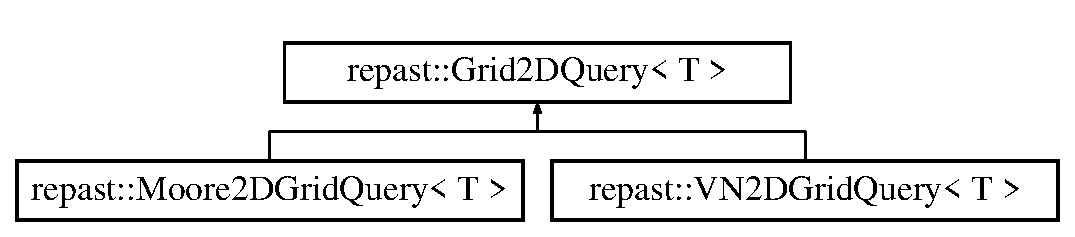
\includegraphics[height=2.000000cm]{classrepast_1_1_grid2_d_query}
\end{center}
\end{figure}
\subsection*{Public Member Functions}
\begin{DoxyCompactItemize}
\item 
\hypertarget{classrepast_1_1_grid2_d_query_a53b52f9a510b9ca3b2a98de26761ab00}{\hyperlink{classrepast_1_1_grid2_d_query_a53b52f9a510b9ca3b2a98de26761ab00}{Grid2\-D\-Query} (const \hyperlink{classrepast_1_1_grid}{Grid}$<$ T, int $>$ $\ast$grid)}\label{classrepast_1_1_grid2_d_query_a53b52f9a510b9ca3b2a98de26761ab00}

\begin{DoxyCompactList}\small\item\em Creates \hyperlink{classrepast_1_1_grid2_d_query}{Grid2\-D\-Query} that will query the specified \hyperlink{classrepast_1_1_grid}{Grid}. \end{DoxyCompactList}\item 
virtual void \hyperlink{classrepast_1_1_grid2_d_query_a44d46360d72ba9e7b0114c2cb248ee96}{query} (const \hyperlink{classrepast_1_1_point}{Point}$<$ int $>$ \&center, int range, bool include\-Center, std\-::vector$<$ T $\ast$ $>$ \&out) const =0
\begin{DoxyCompactList}\small\item\em Queries the \hyperlink{classrepast_1_1_grid}{Grid} for the neighbors surrounding the center point within a specified range. \end{DoxyCompactList}\end{DoxyCompactItemize}
\subsection*{Protected Attributes}
\begin{DoxyCompactItemize}
\item 
\hypertarget{classrepast_1_1_grid2_d_query_a658f6f194ed9ed44f32ebe413f063b0b}{const \hyperlink{classrepast_1_1_grid}{Grid}$<$ T, int $>$ $\ast$ {\bfseries \-\_\-grid}}\label{classrepast_1_1_grid2_d_query_a658f6f194ed9ed44f32ebe413f063b0b}

\item 
\hypertarget{classrepast_1_1_grid2_d_query_a63e0a5851f9045821f89bd8a16daedf5}{int {\bfseries min\-Max} \mbox{[}2\mbox{]}\mbox{[}2\mbox{]}}\label{classrepast_1_1_grid2_d_query_a63e0a5851f9045821f89bd8a16daedf5}

\end{DoxyCompactItemize}


\subsection{Detailed Description}
\subsubsection*{template$<$typename T$>$class repast\-::\-Grid2\-D\-Query$<$ T $>$}

Base class for neighborhood queries on discrete Grids. 


\begin{DoxyTemplParams}{Template Parameters}
{\em T} & the type of object in the \hyperlink{classrepast_1_1_grid}{Grid}. \\
\hline
\end{DoxyTemplParams}


\subsection{Member Function Documentation}
\hypertarget{classrepast_1_1_grid2_d_query_a44d46360d72ba9e7b0114c2cb248ee96}{\index{repast\-::\-Grid2\-D\-Query@{repast\-::\-Grid2\-D\-Query}!query@{query}}
\index{query@{query}!repast::Grid2DQuery@{repast\-::\-Grid2\-D\-Query}}
\subsubsection[{query}]{\setlength{\rightskip}{0pt plus 5cm}template$<$typename T $>$ virtual void {\bf repast\-::\-Grid2\-D\-Query}$<$ T $>$\-::query (
\begin{DoxyParamCaption}
\item[{const {\bf Point}$<$ int $>$ \&}]{center, }
\item[{int}]{range, }
\item[{bool}]{include\-Center, }
\item[{std\-::vector$<$ T $\ast$ $>$ \&}]{out}
\end{DoxyParamCaption}
) const\hspace{0.3cm}{\ttfamily [pure virtual]}}}\label{classrepast_1_1_grid2_d_query_a44d46360d72ba9e7b0114c2cb248ee96}


Queries the \hyperlink{classrepast_1_1_grid}{Grid} for the neighbors surrounding the center point within a specified range. 

What constitutes the neighborhood is determines by subclass implementors.


\begin{DoxyParams}[1]{Parameters}
 & {\em center} & the center of the neighborhood \\
\hline
 & {\em range} & the range of the neighborhood out from the center \\
\hline
 & {\em include\-Center} & whether or not to include any agents at the center \\
\hline
\mbox{\tt out}  & {\em the} & neighboring agents will be returned in this vector \\
\hline
\end{DoxyParams}


Implemented in \hyperlink{classrepast_1_1_moore2_d_grid_query_a43cd6c0a6cd2c3f1932bbaa5595b0576}{repast\-::\-Moore2\-D\-Grid\-Query$<$ T $>$}, and \hyperlink{classrepast_1_1_v_n2_d_grid_query_a650d78bb1a0038e0f676121e90052873}{repast\-::\-V\-N2\-D\-Grid\-Query$<$ T $>$}.



The documentation for this class was generated from the following file\-:\begin{DoxyCompactItemize}
\item 
repast\-\_\-hpc/Grid2\-D\-Query.\-h\end{DoxyCompactItemize}

\hypertarget{classrepast_1_1_grid_buffer_syncher}{\section{repast\-:\-:Grid\-Buffer\-Syncher$<$ T, G\-P\-Type $>$ Class Template Reference}
\label{classrepast_1_1_grid_buffer_syncher}\index{repast\-::\-Grid\-Buffer\-Syncher$<$ T, G\-P\-Type $>$@{repast\-::\-Grid\-Buffer\-Syncher$<$ T, G\-P\-Type $>$}}
}


{\itshape D\-E\-P\-R\-E\-C\-A\-T\-E\-D} Helper class that provides support for synchronizing a grid / space buffer.  




{\ttfamily \#include $<$Shared\-Base\-Grid.\-h$>$}

\subsection*{Public Member Functions}
\begin{DoxyCompactItemize}
\item 
\hypertarget{classrepast_1_1_grid_buffer_syncher_aaf711d6b9a5f8b750bb38fc760ee7e65}{{\bfseries Grid\-Buffer\-Syncher} (boost\-::mpi\-::communicator $\ast$world)}\label{classrepast_1_1_grid_buffer_syncher_aaf711d6b9a5f8b750bb38fc760ee7e65}

\item 
\hypertarget{classrepast_1_1_grid_buffer_syncher_a5a88d5fff52263ed26570b802f4e2e52}{std\-::vector$<$ \hyperlink{classrepast_1_1_cell_contents}{Cell\-Contents}$<$ T, \\*
G\-P\-Type $>$ $>$ $\ast$ {\bfseries received} (size\-\_\-t index)}\label{classrepast_1_1_grid_buffer_syncher_a5a88d5fff52263ed26570b802f4e2e52}

\item 
\hypertarget{classrepast_1_1_grid_buffer_syncher_a3c75891d740c7ffdb106acd0c6a3e18a}{int {\bfseries ngh\-Rank} (size\-\_\-t index)}\label{classrepast_1_1_grid_buffer_syncher_a3c75891d740c7ffdb106acd0c6a3e18a}

\item 
\hypertarget{classrepast_1_1_grid_buffer_syncher_a1feaa3f70fc5db8ce2fccad2c5bee27c}{size\-\_\-t {\bfseries vecs\-Size} ()}\label{classrepast_1_1_grid_buffer_syncher_a1feaa3f70fc5db8ce2fccad2c5bee27c}

\item 
\hypertarget{classrepast_1_1_grid_buffer_syncher_a1a59baa51352a07463176273b1c95901}{void \hyperlink{classrepast_1_1_grid_buffer_syncher_a1a59baa51352a07463176273b1c95901}{send} (int rank, std\-::vector$<$ \hyperlink{classrepast_1_1_cell_contents}{Cell\-Contents}$<$ T, G\-P\-Type $>$ $>$ \&contents, int tag)}\label{classrepast_1_1_grid_buffer_syncher_a1a59baa51352a07463176273b1c95901}

\begin{DoxyCompactList}\small\item\em Sends the contents to the rank. \end{DoxyCompactList}\item 
\hypertarget{classrepast_1_1_grid_buffer_syncher_a2041ea31696f1c0922958f3f09e487b0}{void {\bfseries receive} (\hyperlink{classrepast_1_1_neighbor}{Neighbor} $\ast$ngh, int tag)}\label{classrepast_1_1_grid_buffer_syncher_a2041ea31696f1c0922958f3f09e487b0}

\item 
\hypertarget{classrepast_1_1_grid_buffer_syncher_a5e27b0d4c39471d000bcafb5e5c0fae4}{void {\bfseries wait} ()}\label{classrepast_1_1_grid_buffer_syncher_a5e27b0d4c39471d000bcafb5e5c0fae4}

\end{DoxyCompactItemize}


\subsection{Detailed Description}
\subsubsection*{template$<$typename T, typename G\-P\-Type$>$class repast\-::\-Grid\-Buffer\-Syncher$<$ T, G\-P\-Type $>$}

{\itshape D\-E\-P\-R\-E\-C\-A\-T\-E\-D} Helper class that provides support for synchronizing a grid / space buffer. 

\begin{DoxyRefDesc}{Deprecated}
\item[\hyperlink{deprecated__deprecated000002}{Deprecated}]As of Version 2.\-0 \end{DoxyRefDesc}


The documentation for this class was generated from the following file\-:\begin{DoxyCompactItemize}
\item 
repast\-\_\-hpc/Shared\-Base\-Grid.\-h\end{DoxyCompactItemize}

\hypertarget{classrepast_1_1_grid_dimensions}{\section{repast\-:\-:Grid\-Dimensions Class Reference}
\label{classrepast_1_1_grid_dimensions}\index{repast\-::\-Grid\-Dimensions@{repast\-::\-Grid\-Dimensions}}
}


Basic structure for specifying grid dimenions.  




{\ttfamily \#include $<$Grid\-Dimensions.\-h$>$}

\subsection*{Public Member Functions}
\begin{DoxyCompactItemize}
\item 
\hypertarget{classrepast_1_1_grid_dimensions_adc34342afddc8f1c2c0267522d4594f4}{{\bfseries Grid\-Dimensions} (\hyperlink{classrepast_1_1_point}{Point}$<$ double $>$ extent)}\label{classrepast_1_1_grid_dimensions_adc34342afddc8f1c2c0267522d4594f4}

\item 
\hypertarget{classrepast_1_1_grid_dimensions_a91dde52d1be653a287307ba3c5293346}{\hyperlink{classrepast_1_1_grid_dimensions_a91dde52d1be653a287307ba3c5293346}{Grid\-Dimensions} (\hyperlink{classrepast_1_1_point}{Point}$<$ double $>$ \hyperlink{classrepast_1_1_grid_dimensions_a0ec32ce3994e9903af7068aa9fd3f0f6}{origin}, \hyperlink{classrepast_1_1_point}{Point}$<$ double $>$ extent)}\label{classrepast_1_1_grid_dimensions_a91dde52d1be653a287307ba3c5293346}

\begin{DoxyCompactList}\small\item\em Creates a \hyperlink{classrepast_1_1_grid_dimensions}{Grid\-Dimensions} with the specified origin and extent. \end{DoxyCompactList}\item 
\hypertarget{classrepast_1_1_grid_dimensions_ae258f35627445ba18afeb302dde7f379}{bool {\bfseries contains} (const \hyperlink{classrepast_1_1_point}{Point}$<$ int $>$ \&pt) const }\label{classrepast_1_1_grid_dimensions_ae258f35627445ba18afeb302dde7f379}

\item 
\hypertarget{classrepast_1_1_grid_dimensions_a20572ae249735726419f0183cb2f41cd}{bool {\bfseries contains} (const std\-::vector$<$ int $>$ \&pt) const }\label{classrepast_1_1_grid_dimensions_a20572ae249735726419f0183cb2f41cd}

\item 
\hypertarget{classrepast_1_1_grid_dimensions_ac364611e0c8dd54b0df8ef753a1c3080}{bool {\bfseries contains} (const \hyperlink{classrepast_1_1_point}{Point}$<$ double $>$ \&pt) const }\label{classrepast_1_1_grid_dimensions_ac364611e0c8dd54b0df8ef753a1c3080}

\item 
\hypertarget{classrepast_1_1_grid_dimensions_ab1f3412888524fab6d6c3c517b27da85}{bool {\bfseries contains} (const std\-::vector$<$ double $>$ \&pt) const }\label{classrepast_1_1_grid_dimensions_ab1f3412888524fab6d6c3c517b27da85}

\item 
\hypertarget{classrepast_1_1_grid_dimensions_a0ec32ce3994e9903af7068aa9fd3f0f6}{const \hyperlink{classrepast_1_1_point}{Point}$<$ double $>$ \& \hyperlink{classrepast_1_1_grid_dimensions_a0ec32ce3994e9903af7068aa9fd3f0f6}{origin} () const }\label{classrepast_1_1_grid_dimensions_a0ec32ce3994e9903af7068aa9fd3f0f6}

\begin{DoxyCompactList}\small\item\em Gets the origin. \end{DoxyCompactList}\item 
\hypertarget{classrepast_1_1_grid_dimensions_abd4875c315a9420c18f0c369f3a8af9a}{const \hyperlink{classrepast_1_1_point}{Point}$<$ double $>$ \& \hyperlink{classrepast_1_1_grid_dimensions_abd4875c315a9420c18f0c369f3a8af9a}{extents} () const }\label{classrepast_1_1_grid_dimensions_abd4875c315a9420c18f0c369f3a8af9a}

\begin{DoxyCompactList}\small\item\em Gets the extents along each dimension. \end{DoxyCompactList}\item 
\hypertarget{classrepast_1_1_grid_dimensions_ac30a2660eff0158ca306fcff807f57a7}{const double \& {\bfseries origin} (int index) const }\label{classrepast_1_1_grid_dimensions_ac30a2660eff0158ca306fcff807f57a7}

\item 
\hypertarget{classrepast_1_1_grid_dimensions_ae7104e85e069a7108eba8db95ad11a54}{const double \& {\bfseries extents} (int index) const }\label{classrepast_1_1_grid_dimensions_ae7104e85e069a7108eba8db95ad11a54}

\item 
\hypertarget{classrepast_1_1_grid_dimensions_a7961c67064727f34d52045385517c024}{size\-\_\-t {\bfseries dimension\-Count} () const }\label{classrepast_1_1_grid_dimensions_a7961c67064727f34d52045385517c024}

\end{DoxyCompactItemize}
\subsection*{Friends}
\begin{DoxyCompactItemize}
\item 
\hypertarget{classrepast_1_1_grid_dimensions_aba42531b113bed80dcac86aac0377225}{bool {\bfseries operator==} (const \hyperlink{classrepast_1_1_grid_dimensions}{Grid\-Dimensions} \&one, const \hyperlink{classrepast_1_1_grid_dimensions}{Grid\-Dimensions} \&two)}\label{classrepast_1_1_grid_dimensions_aba42531b113bed80dcac86aac0377225}

\item 
\hypertarget{classrepast_1_1_grid_dimensions_aca04c2784205aba66e1478fdfdbb24db}{std\-::ostream \& {\bfseries operator$<$$<$} (std\-::ostream \&os, const \hyperlink{classrepast_1_1_grid_dimensions}{Grid\-Dimensions} \&dimensions)}\label{classrepast_1_1_grid_dimensions_aca04c2784205aba66e1478fdfdbb24db}

\end{DoxyCompactItemize}


\subsection{Detailed Description}
Basic structure for specifying grid dimenions. 

Structure is to specify (using instances of \hyperlink{classrepast_1_1_point}{Point}) the origin and the extent, so that an origin of (-\/100, -\/100) and an extent of (200, 200) represents a rectangle with corners at (-\/100, -\/100), (-\/100, 100), (100, 100), and (100, -\/100). 

The documentation for this class was generated from the following files\-:\begin{DoxyCompactItemize}
\item 
repast\-\_\-hpc/Grid\-Dimensions.\-h\item 
repast\-\_\-hpc/Grid\-Dimensions.\-cpp\end{DoxyCompactItemize}

\hypertarget{structrepast_1_1_grid_move_packet}{\section{repast\-:\-:Grid\-Move\-Packet$<$ Pt\-Type $>$ Struct Template Reference}
\label{structrepast_1_1_grid_move_packet}\index{repast\-::\-Grid\-Move\-Packet$<$ Pt\-Type $>$@{repast\-::\-Grid\-Move\-Packet$<$ Pt\-Type $>$}}
}


Encapsulates info about an agent moving off the grid\-: the rank it moved to, its grid location, and the agent id.  




{\ttfamily \#include $<$Grid\-Move\-Packets.\-h$>$}

\subsection*{Public Member Functions}
\begin{DoxyCompactItemize}
\item 
\hypertarget{structrepast_1_1_grid_move_packet_a72a97c5b7298dc21c12ed462f34f3abf}{{\bfseries Grid\-Move\-Packet} (const \hyperlink{classrepast_1_1_point}{Point}$<$ Pt\-Type $>$ \&pt, const \hyperlink{classrepast_1_1_agent_id}{Agent\-Id} \&id, int rank)}\label{structrepast_1_1_grid_move_packet_a72a97c5b7298dc21c12ed462f34f3abf}

\item 
\hypertarget{structrepast_1_1_grid_move_packet_a616996fc4caa27fc8b39042d57949d82}{{\footnotesize template$<$class Archive $>$ }\\void {\bfseries serialize} (Archive \&ar, const unsigned int version)}\label{structrepast_1_1_grid_move_packet_a616996fc4caa27fc8b39042d57949d82}

\end{DoxyCompactItemize}
\subsection*{Public Attributes}
\begin{DoxyCompactItemize}
\item 
\hypertarget{structrepast_1_1_grid_move_packet_aa6c737c40abca83df760661a558ba8b3}{\hyperlink{classrepast_1_1_point}{Point}$<$ Pt\-Type $>$ {\bfseries \-\_\-pt}}\label{structrepast_1_1_grid_move_packet_aa6c737c40abca83df760661a558ba8b3}

\item 
\hypertarget{structrepast_1_1_grid_move_packet_ace518a4ce7056ce51a108731273e2807}{\hyperlink{classrepast_1_1_agent_id}{Agent\-Id} {\bfseries \-\_\-id}}\label{structrepast_1_1_grid_move_packet_ace518a4ce7056ce51a108731273e2807}

\item 
\hypertarget{structrepast_1_1_grid_move_packet_ac6b40e29aef48809fb684a88036e61cb}{int {\bfseries \-\_\-rank}}\label{structrepast_1_1_grid_move_packet_ac6b40e29aef48809fb684a88036e61cb}

\end{DoxyCompactItemize}


\subsection{Detailed Description}
\subsubsection*{template$<$typename Pt\-Type$>$struct repast\-::\-Grid\-Move\-Packet$<$ Pt\-Type $>$}

Encapsulates info about an agent moving off the grid\-: the rank it moved to, its grid location, and the agent id. 

The documentation for this struct was generated from the following file\-:\begin{DoxyCompactItemize}
\item 
repast\-\_\-hpc/Grid\-Move\-Packets.\-h\end{DoxyCompactItemize}

\hypertarget{classrepast_1_1_grid_move_packets}{\section{repast\-:\-:Grid\-Move\-Packets$<$ Pt\-Type $>$ Class Template Reference}
\label{classrepast_1_1_grid_move_packets}\index{repast\-::\-Grid\-Move\-Packets$<$ Pt\-Type $>$@{repast\-::\-Grid\-Move\-Packets$<$ Pt\-Type $>$}}
}


A collection of \hyperlink{structrepast_1_1_grid_move_packet}{Grid\-Move\-Packet} objects, kept in a map per destination process.  




{\ttfamily \#include $<$Grid\-Move\-Packets.\-h$>$}

\subsection*{Public Member Functions}
\begin{DoxyCompactItemize}
\item 
\hypertarget{classrepast_1_1_grid_move_packets_a8bc8af3fd01e9896508a70a6681c7fb2}{void {\bfseries add\-Packet} (const \hyperlink{structrepast_1_1_grid_move_packet}{Grid\-Move\-Packet}$<$ Pt\-Type $>$ \&packet)}\label{classrepast_1_1_grid_move_packets_a8bc8af3fd01e9896508a70a6681c7fb2}

\item 
\hypertarget{classrepast_1_1_grid_move_packets_a6c54ec55d5bb7145c4e76583b0f6c4df}{void {\bfseries clear} ()}\label{classrepast_1_1_grid_move_packets_a6c54ec55d5bb7145c4e76583b0f6c4df}

\item 
\hypertarget{classrepast_1_1_grid_move_packets_aabe5f41d7a3b20e17ef58423d51b8acf}{void \hyperlink{classrepast_1_1_grid_move_packets_aabe5f41d7a3b20e17ef58423d51b8acf}{remove\-Packet\-For} (const \hyperlink{classrepast_1_1_agent_id}{Agent\-Id} \&id)}\label{classrepast_1_1_grid_move_packets_aabe5f41d7a3b20e17ef58423d51b8acf}

\begin{DoxyCompactList}\small\item\em Removes any Grid\-Move\-Packet-\/s associated with the specified agent id. \end{DoxyCompactList}\item 
\hypertarget{classrepast_1_1_grid_move_packets_a87a42bb21680295cbc11f5f7dcc86b80}{void {\bfseries send} (std\-::vector$<$ boost\-::mpi\-::request $>$ \&requests, boost\-::mpi\-::communicator world)}\label{classrepast_1_1_grid_move_packets_a87a42bb21680295cbc11f5f7dcc86b80}

\item 
\hypertarget{classrepast_1_1_grid_move_packets_a42c07125961b39ee4ef64b933cb546a0}{void {\bfseries receivers} (std\-::vector$<$ int $>$ \&receivers)}\label{classrepast_1_1_grid_move_packets_a42c07125961b39ee4ef64b933cb546a0}

\end{DoxyCompactItemize}


\subsection{Detailed Description}
\subsubsection*{template$<$typename Pt\-Type$>$class repast\-::\-Grid\-Move\-Packets$<$ Pt\-Type $>$}

A collection of \hyperlink{structrepast_1_1_grid_move_packet}{Grid\-Move\-Packet} objects, kept in a map per destination process. 

The documentation for this class was generated from the following file\-:\begin{DoxyCompactItemize}
\item 
repast\-\_\-hpc/Grid\-Move\-Packets.\-h\end{DoxyCompactItemize}

\hypertarget{structrepast_1_1_grid_point_holder}{\section{repast\-:\-:Grid\-Point\-Holder$<$ T, G\-P\-Type $>$ Struct Template Reference}
\label{structrepast_1_1_grid_point_holder}\index{repast\-::\-Grid\-Point\-Holder$<$ T, G\-P\-Type $>$@{repast\-::\-Grid\-Point\-Holder$<$ T, G\-P\-Type $>$}}
}


Encapsulates a grid point and what is held in it.  




{\ttfamily \#include $<$Base\-Grid.\-h$>$}

\subsection*{Public Attributes}
\begin{DoxyCompactItemize}
\item 
\hypertarget{structrepast_1_1_grid_point_holder_a11a11a29f6d73f6766a18ce83b9404a3}{bool {\bfseries in\-Grid}}\label{structrepast_1_1_grid_point_holder_a11a11a29f6d73f6766a18ce83b9404a3}

\item 
\hypertarget{structrepast_1_1_grid_point_holder_a9a290fdba30d1ea6de4f4314f52c2012}{\hyperlink{classrepast_1_1_point}{Point}$<$ G\-P\-Type $>$ {\bfseries point}}\label{structrepast_1_1_grid_point_holder_a9a290fdba30d1ea6de4f4314f52c2012}

\item 
\hypertarget{structrepast_1_1_grid_point_holder_a2f250cd6c9542010610957b75b8ff088}{boost\-::shared\-\_\-ptr$<$ T $>$ {\bfseries ptr}}\label{structrepast_1_1_grid_point_holder_a2f250cd6c9542010610957b75b8ff088}

\end{DoxyCompactItemize}


\subsection{Detailed Description}
\subsubsection*{template$<$typename T, typename G\-P\-Type$>$struct repast\-::\-Grid\-Point\-Holder$<$ T, G\-P\-Type $>$}

Encapsulates a grid point and what is held in it. 

The documentation for this struct was generated from the following file\-:\begin{DoxyCompactItemize}
\item 
repast\-\_\-hpc/Base\-Grid.\-h\end{DoxyCompactItemize}

\hypertarget{structrepast_1_1_hash_grid_point}{\section{repast\-:\-:Hash\-Grid\-Point$<$ T $>$ Struct Template Reference}
\label{structrepast_1_1_hash_grid_point}\index{repast\-::\-Hash\-Grid\-Point$<$ T $>$@{repast\-::\-Hash\-Grid\-Point$<$ T $>$}}
}


Class that allows retrieval of hash value for \hyperlink{classrepast_1_1_point}{Point} objects.  




{\ttfamily \#include $<$Point.\-h$>$}

\subsection*{Public Member Functions}
\begin{DoxyCompactItemize}
\item 
\hypertarget{structrepast_1_1_hash_grid_point_a9fad86917c52a2719abe4ef8ca0167fa}{std\-::size\-\_\-t {\bfseries operator()} (const \hyperlink{classrepast_1_1_point}{Point}$<$ T $>$ \&pt) const }\label{structrepast_1_1_hash_grid_point_a9fad86917c52a2719abe4ef8ca0167fa}

\end{DoxyCompactItemize}


\subsection{Detailed Description}
\subsubsection*{template$<$typename T$>$struct repast\-::\-Hash\-Grid\-Point$<$ T $>$}

Class that allows retrieval of hash value for \hyperlink{classrepast_1_1_point}{Point} objects. 

The documentation for this struct was generated from the following file\-:\begin{DoxyCompactItemize}
\item 
repast\-\_\-hpc/Point.\-h\end{DoxyCompactItemize}

\hypertarget{structrepast_1_1_hash_id}{\section{repast\-:\-:Hash\-Id Struct Reference}
\label{structrepast_1_1_hash_id}\index{repast\-::\-Hash\-Id@{repast\-::\-Hash\-Id}}
}


operator() implementation that returns the hashcode of an \hyperlink{classrepast_1_1_agent_id}{Agent\-Id}.  




{\ttfamily \#include $<$Agent\-Id.\-h$>$}

\subsection*{Public Member Functions}
\begin{DoxyCompactItemize}
\item 
\hypertarget{structrepast_1_1_hash_id_a202dfae6a775fc9189f0810a6cdfc329}{std\-::size\-\_\-t {\bfseries operator()} (const \hyperlink{classrepast_1_1_agent_id}{Agent\-Id} \&id) const }\label{structrepast_1_1_hash_id_a202dfae6a775fc9189f0810a6cdfc329}

\end{DoxyCompactItemize}


\subsection{Detailed Description}
operator() implementation that returns the hashcode of an \hyperlink{classrepast_1_1_agent_id}{Agent\-Id}. 

The documentation for this struct was generated from the following file\-:\begin{DoxyCompactItemize}
\item 
repast\-\_\-hpc/Agent\-Id.\-h\end{DoxyCompactItemize}

\hypertarget{structrepast_1_1_hash_vertex}{\section{repast\-:\-:Hash\-Vertex$<$ V, E $>$ Struct Template Reference}
\label{structrepast_1_1_hash_vertex}\index{repast\-::\-Hash\-Vertex$<$ V, E $>$@{repast\-::\-Hash\-Vertex$<$ V, E $>$}}
}


Hashes a \hyperlink{classrepast_1_1_vertex}{Vertex} using the hashcode of the \hyperlink{classrepast_1_1_agent_id}{Agent\-Id} that the vertex contains.  




{\ttfamily \#include $<$Vertex.\-h$>$}

\subsection*{Public Member Functions}
\begin{DoxyCompactItemize}
\item 
\hypertarget{structrepast_1_1_hash_vertex_a675c035c3939548181bce7e09bcb01b0}{std\-::size\-\_\-t {\bfseries operator()} (\hyperlink{classrepast_1_1_vertex}{Vertex}$<$ V, E $>$ $\ast$vertex) const }\label{structrepast_1_1_hash_vertex_a675c035c3939548181bce7e09bcb01b0}

\end{DoxyCompactItemize}


\subsection{Detailed Description}
\subsubsection*{template$<$typename V, typename E$>$struct repast\-::\-Hash\-Vertex$<$ V, E $>$}

Hashes a \hyperlink{classrepast_1_1_vertex}{Vertex} using the hashcode of the \hyperlink{classrepast_1_1_agent_id}{Agent\-Id} that the vertex contains. 

The documentation for this struct was generated from the following file\-:\begin{DoxyCompactItemize}
\item 
repast\-\_\-hpc/Vertex.\-h\end{DoxyCompactItemize}

\hypertarget{classrepast_1_1_importer___c_o_u_n_t}{\section{repast\-:\-:Importer\-\_\-\-C\-O\-U\-N\-T Class Reference}
\label{classrepast_1_1_importer___c_o_u_n_t}\index{repast\-::\-Importer\-\_\-\-C\-O\-U\-N\-T@{repast\-::\-Importer\-\_\-\-C\-O\-U\-N\-T}}
}


Importer that maintains a simple count of the agents being sent from each sending process.  




{\ttfamily \#include $<$Agent\-Importer\-Exporter.\-h$>$}

Inheritance diagram for repast\-:\-:Importer\-\_\-\-C\-O\-U\-N\-T\-:\begin{figure}[H]
\begin{center}
\leavevmode
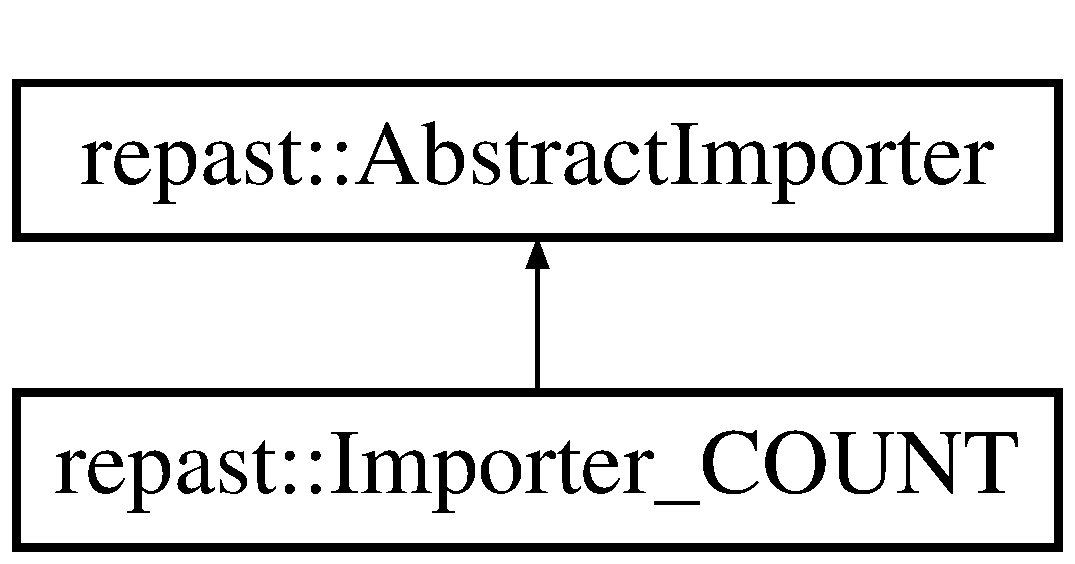
\includegraphics[height=2.000000cm]{classrepast_1_1_importer___c_o_u_n_t}
\end{center}
\end{figure}
\subsection*{Public Member Functions}
\begin{DoxyCompactItemize}
\item 
virtual void \hyperlink{classrepast_1_1_importer___c_o_u_n_t_a37a926665920b7674009603f6512b40e}{register\-Outgoing\-Requests} (\hyperlink{classrepast_1_1_agent_request}{Agent\-Request} \&req)
\begin{DoxyCompactList}\small\item\em Given an agent request (including requests for agents on multiple other processes), makes a record of the agents that are being requested by this process and will therefore be received from other processes. \end{DoxyCompactList}\item 
\hypertarget{classrepast_1_1_importer___c_o_u_n_t_a9cd432b326b3fb476fbbcc8e8dae99ca}{virtual void \hyperlink{classrepast_1_1_importer___c_o_u_n_t_a9cd432b326b3fb476fbbcc8e8dae99ca}{imported\-Agent\-Is\-Removed} (const \hyperlink{classrepast_1_1_agent_id}{Agent\-Id} \&id)}\label{classrepast_1_1_importer___c_o_u_n_t_a9cd432b326b3fb476fbbcc8e8dae99ca}

\begin{DoxyCompactList}\small\item\em Notifies this importer that the agent that it (presumably) has been importing has been removed from the simulation on its home process, and the information for that agent will no longer be sent. \end{DoxyCompactList}\item 
\hypertarget{classrepast_1_1_importer___c_o_u_n_t_a3e766c3fed551067d4c410140181d123}{virtual void \hyperlink{classrepast_1_1_importer___c_o_u_n_t_a3e766c3fed551067d4c410140181d123}{imported\-Agent\-Is\-Moved} (const \hyperlink{classrepast_1_1_agent_id}{Agent\-Id} \&id, int new\-Process)}\label{classrepast_1_1_importer___c_o_u_n_t_a3e766c3fed551067d4c410140181d123}

\begin{DoxyCompactList}\small\item\em Notifies this importer that the agent that it (presumably) has been importing from another process has been moved; its information will now be received from its new home process (unless the agent was moved to this process) \end{DoxyCompactList}\item 
\hypertarget{classrepast_1_1_importer___c_o_u_n_t_ac1096784c7d1255830cbf6507f768f74}{virtual std\-::string \hyperlink{classrepast_1_1_importer___c_o_u_n_t_ac1096784c7d1255830cbf6507f768f74}{get\-Report} ()}\label{classrepast_1_1_importer___c_o_u_n_t_ac1096784c7d1255830cbf6507f768f74}

\begin{DoxyCompactList}\small\item\em Get a printable indication of the data in this object. \end{DoxyCompactList}\item 
\hypertarget{classrepast_1_1_importer___c_o_u_n_t_a71c4c687cfefcd2509143868b644578a}{virtual void {\bfseries get\-Set\-Of\-Agents\-Being\-Imported} (std\-::set$<$ \hyperlink{classrepast_1_1_agent_id}{Agent\-Id} $>$ \&set)}\label{classrepast_1_1_importer___c_o_u_n_t_a71c4c687cfefcd2509143868b644578a}

\end{DoxyCompactItemize}
\subsection*{Additional Inherited Members}


\subsection{Detailed Description}
Importer that maintains a simple count of the agents being sent from each sending process. 

When the count for a given process is zero no mpi 'receive' is created for that process; when the count is nonzero, a 'receive' is created. Note that no record of which agents are requested is kept, only the count of agents requested is kept. 

\subsection{Member Function Documentation}
\hypertarget{classrepast_1_1_importer___c_o_u_n_t_a37a926665920b7674009603f6512b40e}{\index{repast\-::\-Importer\-\_\-\-C\-O\-U\-N\-T@{repast\-::\-Importer\-\_\-\-C\-O\-U\-N\-T}!register\-Outgoing\-Requests@{register\-Outgoing\-Requests}}
\index{register\-Outgoing\-Requests@{register\-Outgoing\-Requests}!repast::Importer_COUNT@{repast\-::\-Importer\-\_\-\-C\-O\-U\-N\-T}}
\subsubsection[{register\-Outgoing\-Requests}]{\setlength{\rightskip}{0pt plus 5cm}void Importer\-\_\-\-C\-O\-U\-N\-T\-::register\-Outgoing\-Requests (
\begin{DoxyParamCaption}
\item[{{\bf Agent\-Request} \&}]{req}
\end{DoxyParamCaption}
)\hspace{0.3cm}{\ttfamily [virtual]}}}\label{classrepast_1_1_importer___c_o_u_n_t_a37a926665920b7674009603f6512b40e}


Given an agent request (including requests for agents on multiple other processes), makes a record of the agents that are being requested by this process and will therefore be received from other processes. 

The record must at a minimum indicate which other processes are sending agent information, but may include other information, such as how many times a particular agent has been requested. 

Implements \hyperlink{classrepast_1_1_abstract_importer_a1353cfde773ce5b3e7011571aff1f823}{repast\-::\-Abstract\-Importer}.



The documentation for this class was generated from the following files\-:\begin{DoxyCompactItemize}
\item 
repast\-\_\-hpc/Agent\-Importer\-Exporter.\-h\item 
repast\-\_\-hpc/Agent\-Importer\-Exporter.\-cpp\end{DoxyCompactItemize}

\hypertarget{classrepast_1_1_importer___l_i_s_t}{\section{repast\-:\-:Importer\-\_\-\-L\-I\-S\-T Class Reference}
\label{classrepast_1_1_importer___l_i_s_t}\index{repast\-::\-Importer\-\_\-\-L\-I\-S\-T@{repast\-::\-Importer\-\_\-\-L\-I\-S\-T}}
}


Importer that maintains a list of the agents being sent from each sending process.  




{\ttfamily \#include $<$Agent\-Importer\-Exporter.\-h$>$}

Inheritance diagram for repast\-:\-:Importer\-\_\-\-L\-I\-S\-T\-:\begin{figure}[H]
\begin{center}
\leavevmode
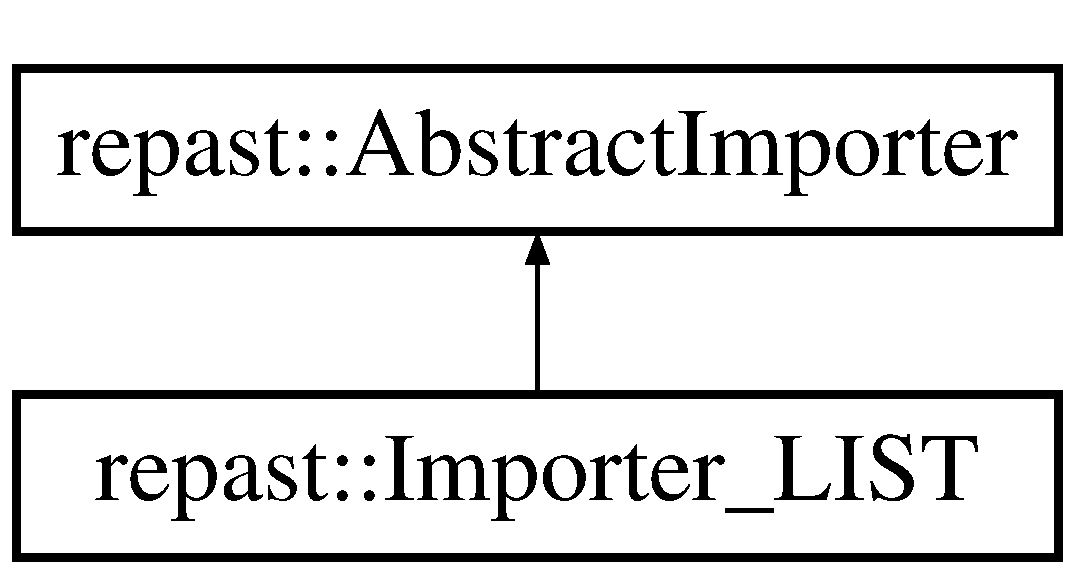
\includegraphics[height=2.000000cm]{classrepast_1_1_importer___l_i_s_t}
\end{center}
\end{figure}
\subsection*{Public Member Functions}
\begin{DoxyCompactItemize}
\item 
virtual void \hyperlink{classrepast_1_1_importer___l_i_s_t_a5be3bf4dda0a23db4727882511e2e224}{register\-Outgoing\-Requests} (\hyperlink{classrepast_1_1_agent_request}{Agent\-Request} \&req)
\begin{DoxyCompactList}\small\item\em Given an agent request (including requests for agents on multiple other processes), makes a record of the agents that are being requested by this process and will therefore be received from other processes. \end{DoxyCompactList}\item 
\hypertarget{classrepast_1_1_importer___l_i_s_t_a9aa7d2da113aaeaa90aaee0b7714b115}{virtual void \hyperlink{classrepast_1_1_importer___l_i_s_t_a9aa7d2da113aaeaa90aaee0b7714b115}{imported\-Agent\-Is\-Removed} (const \hyperlink{classrepast_1_1_agent_id}{Agent\-Id} \&id)}\label{classrepast_1_1_importer___l_i_s_t_a9aa7d2da113aaeaa90aaee0b7714b115}

\begin{DoxyCompactList}\small\item\em Notifies this importer that the agent that it (presumably) has been importing has been removed from the simulation on its home process, and the information for that agent will no longer be sent. \end{DoxyCompactList}\item 
\hypertarget{classrepast_1_1_importer___l_i_s_t_abb7d36027af41cd91cf1e68bfbd84c5c}{virtual void \hyperlink{classrepast_1_1_importer___l_i_s_t_abb7d36027af41cd91cf1e68bfbd84c5c}{imported\-Agent\-Is\-Moved} (const \hyperlink{classrepast_1_1_agent_id}{Agent\-Id} \&id, int new\-Process)}\label{classrepast_1_1_importer___l_i_s_t_abb7d36027af41cd91cf1e68bfbd84c5c}

\begin{DoxyCompactList}\small\item\em Notifies this importer that the agent that it (presumably) has been importing from another process has been moved; its information will now be received from its new home process (unless the agent was moved to this process) \end{DoxyCompactList}\item 
\hypertarget{classrepast_1_1_importer___l_i_s_t_a55e937cfe6eca041b99ba8acc0b2d7c3}{virtual std\-::string \hyperlink{classrepast_1_1_importer___l_i_s_t_a55e937cfe6eca041b99ba8acc0b2d7c3}{get\-Report} ()}\label{classrepast_1_1_importer___l_i_s_t_a55e937cfe6eca041b99ba8acc0b2d7c3}

\begin{DoxyCompactList}\small\item\em Get a printable indication of the data in this object. \end{DoxyCompactList}\item 
\hypertarget{classrepast_1_1_importer___l_i_s_t_a62df237c682e146ddfda6231058554e1}{virtual void {\bfseries get\-Set\-Of\-Agents\-Being\-Imported} (std\-::set$<$ \hyperlink{classrepast_1_1_agent_id}{Agent\-Id} $>$ \&set)}\label{classrepast_1_1_importer___l_i_s_t_a62df237c682e146ddfda6231058554e1}

\item 
\hypertarget{classrepast_1_1_importer___l_i_s_t_a3634bfc0d424dfe72ec886021a8f55d5}{virtual void {\bfseries clear} ()}\label{classrepast_1_1_importer___l_i_s_t_a3634bfc0d424dfe72ec886021a8f55d5}

\end{DoxyCompactItemize}
\subsection*{Additional Inherited Members}


\subsection{Detailed Description}
Importer that maintains a list of the agents being sent from each sending process. 

If there are no agents being sent the size of the list will be zero and no mpi 'receive' will be created; for non-\/zero-\/length lists a single mpi 'receiver' is created. An agent that is requested twice is placed in the list twice. Semantically this means that an agent cancellation will remove the agent from the list exactly once, but also that removing an agent from the list who is not found in the list will not reduce the list size (c.\-f. the 'count' version, where every cancellation reduces the count whether the specific agent being canceled was ever requested at all). 

\subsection{Member Function Documentation}
\hypertarget{classrepast_1_1_importer___l_i_s_t_a5be3bf4dda0a23db4727882511e2e224}{\index{repast\-::\-Importer\-\_\-\-L\-I\-S\-T@{repast\-::\-Importer\-\_\-\-L\-I\-S\-T}!register\-Outgoing\-Requests@{register\-Outgoing\-Requests}}
\index{register\-Outgoing\-Requests@{register\-Outgoing\-Requests}!repast::Importer_LIST@{repast\-::\-Importer\-\_\-\-L\-I\-S\-T}}
\subsubsection[{register\-Outgoing\-Requests}]{\setlength{\rightskip}{0pt plus 5cm}void Importer\-\_\-\-L\-I\-S\-T\-::register\-Outgoing\-Requests (
\begin{DoxyParamCaption}
\item[{{\bf Agent\-Request} \&}]{req}
\end{DoxyParamCaption}
)\hspace{0.3cm}{\ttfamily [virtual]}}}\label{classrepast_1_1_importer___l_i_s_t_a5be3bf4dda0a23db4727882511e2e224}


Given an agent request (including requests for agents on multiple other processes), makes a record of the agents that are being requested by this process and will therefore be received from other processes. 

The record must at a minimum indicate which other processes are sending agent information, but may include other information, such as how many times a particular agent has been requested. 

Implements \hyperlink{classrepast_1_1_abstract_importer_a1353cfde773ce5b3e7011571aff1f823}{repast\-::\-Abstract\-Importer}.



The documentation for this class was generated from the following files\-:\begin{DoxyCompactItemize}
\item 
repast\-\_\-hpc/Agent\-Importer\-Exporter.\-h\item 
repast\-\_\-hpc/Agent\-Importer\-Exporter.\-cpp\end{DoxyCompactItemize}

\hypertarget{classrepast_1_1_importer___m_a_p__int}{\section{repast\-:\-:Importer\-\_\-\-M\-A\-P\-\_\-int Class Reference}
\label{classrepast_1_1_importer___m_a_p__int}\index{repast\-::\-Importer\-\_\-\-M\-A\-P\-\_\-int@{repast\-::\-Importer\-\_\-\-M\-A\-P\-\_\-int}}
}


Importer that maintains a map of agents being sent from each sending process and a count of the number of times that agent was requested.  




{\ttfamily \#include $<$Agent\-Importer\-Exporter.\-h$>$}

Inheritance diagram for repast\-:\-:Importer\-\_\-\-M\-A\-P\-\_\-int\-:\begin{figure}[H]
\begin{center}
\leavevmode
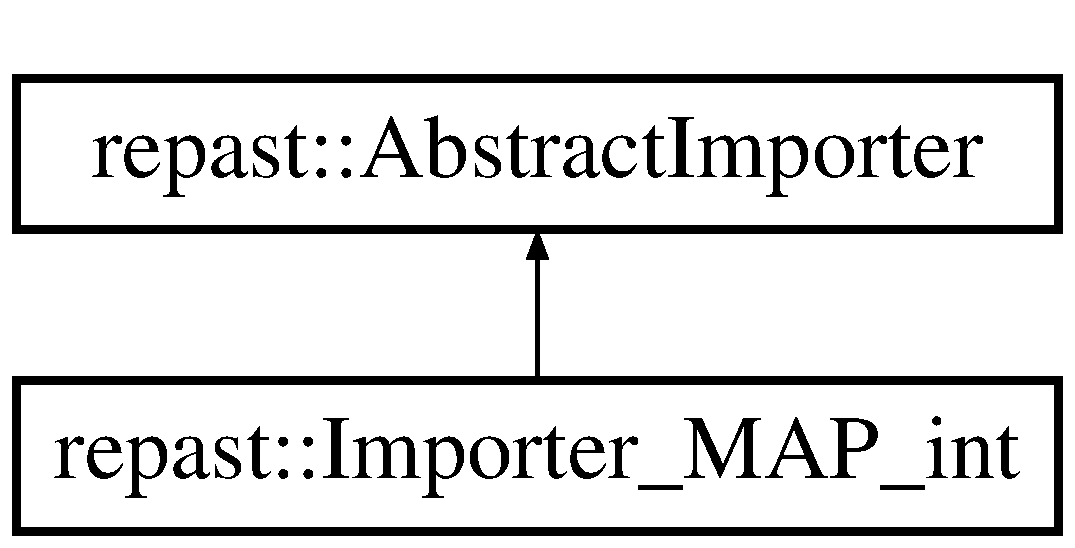
\includegraphics[height=2.000000cm]{classrepast_1_1_importer___m_a_p__int}
\end{center}
\end{figure}
\subsection*{Public Member Functions}
\begin{DoxyCompactItemize}
\item 
virtual void \hyperlink{classrepast_1_1_importer___m_a_p__int_aa68061de5fd367ebac5e3b85d184a8e3}{register\-Outgoing\-Requests} (\hyperlink{classrepast_1_1_agent_request}{Agent\-Request} \&req)
\begin{DoxyCompactList}\small\item\em Given an agent request (including requests for agents on multiple other processes), makes a record of the agents that are being requested by this process and will therefore be received from other processes. \end{DoxyCompactList}\item 
\hypertarget{classrepast_1_1_importer___m_a_p__int_af6464e9b0c879d356df274c66dcc2ab5}{virtual void \hyperlink{classrepast_1_1_importer___m_a_p__int_af6464e9b0c879d356df274c66dcc2ab5}{imported\-Agent\-Is\-Removed} (const \hyperlink{classrepast_1_1_agent_id}{Agent\-Id} \&id)}\label{classrepast_1_1_importer___m_a_p__int_af6464e9b0c879d356df274c66dcc2ab5}

\begin{DoxyCompactList}\small\item\em Notifies this importer that the agent that it (presumably) has been importing has been removed from the simulation on its home process, and the information for that agent will no longer be sent. \end{DoxyCompactList}\item 
\hypertarget{classrepast_1_1_importer___m_a_p__int_ade6655860bbac97d3722f0ae4b862fbc}{virtual void \hyperlink{classrepast_1_1_importer___m_a_p__int_ade6655860bbac97d3722f0ae4b862fbc}{imported\-Agent\-Is\-Moved} (const \hyperlink{classrepast_1_1_agent_id}{Agent\-Id} \&id, int new\-Process)}\label{classrepast_1_1_importer___m_a_p__int_ade6655860bbac97d3722f0ae4b862fbc}

\begin{DoxyCompactList}\small\item\em Notifies this importer that the agent that it (presumably) has been importing from another process has been moved; its information will now be received from its new home process (unless the agent was moved to this process) \end{DoxyCompactList}\item 
\hypertarget{classrepast_1_1_importer___m_a_p__int_ad8df0a52e32613cc93eaf9981e6b6ad0}{virtual std\-::string \hyperlink{classrepast_1_1_importer___m_a_p__int_ad8df0a52e32613cc93eaf9981e6b6ad0}{get\-Report} ()}\label{classrepast_1_1_importer___m_a_p__int_ad8df0a52e32613cc93eaf9981e6b6ad0}

\begin{DoxyCompactList}\small\item\em Get a printable indication of the data in this object. \end{DoxyCompactList}\item 
\hypertarget{classrepast_1_1_importer___m_a_p__int_a3f507ea09dc1d74fcf04e2959f3da113}{virtual void {\bfseries get\-Set\-Of\-Agents\-Being\-Imported} (std\-::set$<$ \hyperlink{classrepast_1_1_agent_id}{Agent\-Id} $>$ \&set)}\label{classrepast_1_1_importer___m_a_p__int_a3f507ea09dc1d74fcf04e2959f3da113}

\item 
\hypertarget{classrepast_1_1_importer___m_a_p__int_ab42558da0dbc7e0553509146e3d75f37}{virtual void {\bfseries clear} ()}\label{classrepast_1_1_importer___m_a_p__int_ab42558da0dbc7e0553509146e3d75f37}

\end{DoxyCompactItemize}
\subsection*{Additional Inherited Members}


\subsection{Detailed Description}
Importer that maintains a map of agents being sent from each sending process and a count of the number of times that agent was requested. 

This is semantically equivalent to a 'L\-I\-S\-T' type, but may be more or less appropriate in specific contexts based on performance. Duplicate requests for an agent increment the count associated with that agent; canceling a request reduces that count. If a given sending process has no agents being shared, no mpi 'receive' will be created, but if there are agents being shared, a 'receive' will be created. 

\subsection{Member Function Documentation}
\hypertarget{classrepast_1_1_importer___m_a_p__int_aa68061de5fd367ebac5e3b85d184a8e3}{\index{repast\-::\-Importer\-\_\-\-M\-A\-P\-\_\-int@{repast\-::\-Importer\-\_\-\-M\-A\-P\-\_\-int}!register\-Outgoing\-Requests@{register\-Outgoing\-Requests}}
\index{register\-Outgoing\-Requests@{register\-Outgoing\-Requests}!repast::Importer_MAP_int@{repast\-::\-Importer\-\_\-\-M\-A\-P\-\_\-int}}
\subsubsection[{register\-Outgoing\-Requests}]{\setlength{\rightskip}{0pt plus 5cm}void Importer\-\_\-\-M\-A\-P\-\_\-int\-::register\-Outgoing\-Requests (
\begin{DoxyParamCaption}
\item[{{\bf Agent\-Request} \&}]{req}
\end{DoxyParamCaption}
)\hspace{0.3cm}{\ttfamily [virtual]}}}\label{classrepast_1_1_importer___m_a_p__int_aa68061de5fd367ebac5e3b85d184a8e3}


Given an agent request (including requests for agents on multiple other processes), makes a record of the agents that are being requested by this process and will therefore be received from other processes. 

The record must at a minimum indicate which other processes are sending agent information, but may include other information, such as how many times a particular agent has been requested. 

Implements \hyperlink{classrepast_1_1_abstract_importer_a1353cfde773ce5b3e7011571aff1f823}{repast\-::\-Abstract\-Importer}.



The documentation for this class was generated from the following files\-:\begin{DoxyCompactItemize}
\item 
repast\-\_\-hpc/Agent\-Importer\-Exporter.\-h\item 
repast\-\_\-hpc/Agent\-Importer\-Exporter.\-cpp\end{DoxyCompactItemize}

\hypertarget{classrepast_1_1_importer___s_e_t}{\section{repast\-:\-:Importer\-\_\-\-S\-E\-T Class Reference}
\label{classrepast_1_1_importer___s_e_t}\index{repast\-::\-Importer\-\_\-\-S\-E\-T@{repast\-::\-Importer\-\_\-\-S\-E\-T}}
}


Importer that maintains a set of agents being sent from each sending process.  




{\ttfamily \#include $<$Agent\-Importer\-Exporter.\-h$>$}

Inheritance diagram for repast\-:\-:Importer\-\_\-\-S\-E\-T\-:\begin{figure}[H]
\begin{center}
\leavevmode
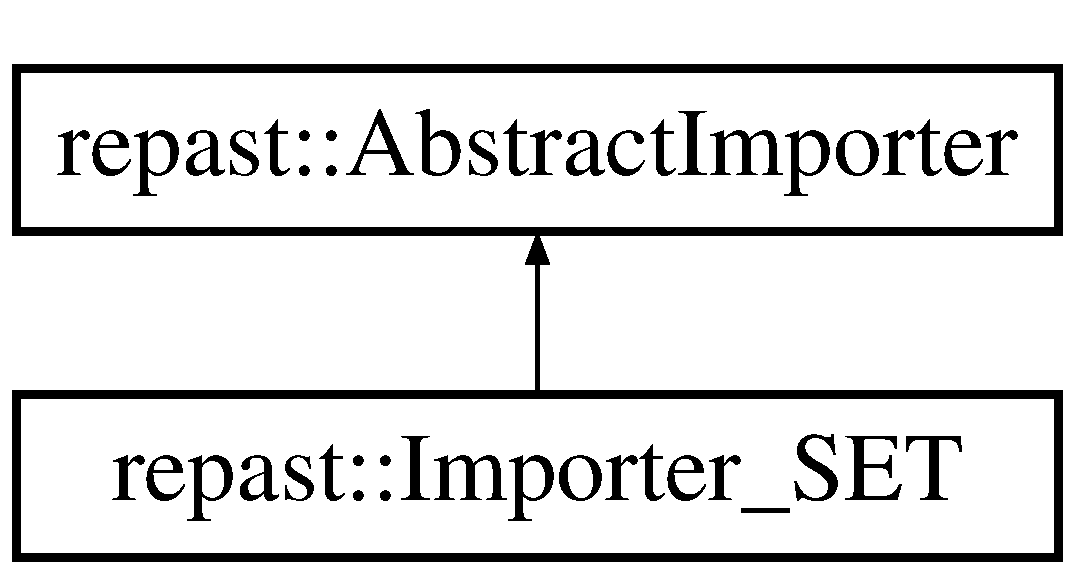
\includegraphics[height=2.000000cm]{classrepast_1_1_importer___s_e_t}
\end{center}
\end{figure}
\subsection*{Public Member Functions}
\begin{DoxyCompactItemize}
\item 
virtual void \hyperlink{classrepast_1_1_importer___s_e_t_a129e0998455430f6036897ab209ef163}{register\-Outgoing\-Requests} (\hyperlink{classrepast_1_1_agent_request}{Agent\-Request} \&req)
\begin{DoxyCompactList}\small\item\em Given an agent request (including requests for agents on multiple other processes), makes a record of the agents that are being requested by this process and will therefore be received from other processes. \end{DoxyCompactList}\item 
\hypertarget{classrepast_1_1_importer___s_e_t_aaf118e0dce13b2db919fdf8c23d4e2dd}{virtual void \hyperlink{classrepast_1_1_importer___s_e_t_aaf118e0dce13b2db919fdf8c23d4e2dd}{imported\-Agent\-Is\-Removed} (const \hyperlink{classrepast_1_1_agent_id}{Agent\-Id} \&id)}\label{classrepast_1_1_importer___s_e_t_aaf118e0dce13b2db919fdf8c23d4e2dd}

\begin{DoxyCompactList}\small\item\em Notifies this importer that the agent that it (presumably) has been importing has been removed from the simulation on its home process, and the information for that agent will no longer be sent. \end{DoxyCompactList}\item 
\hypertarget{classrepast_1_1_importer___s_e_t_a88c897879fd2a5f602237d67a89bd8ab}{virtual void \hyperlink{classrepast_1_1_importer___s_e_t_a88c897879fd2a5f602237d67a89bd8ab}{imported\-Agent\-Is\-Moved} (const \hyperlink{classrepast_1_1_agent_id}{Agent\-Id} \&id, int new\-Process)}\label{classrepast_1_1_importer___s_e_t_a88c897879fd2a5f602237d67a89bd8ab}

\begin{DoxyCompactList}\small\item\em Notifies this importer that the agent that it (presumably) has been importing from another process has been moved; its information will now be received from its new home process (unless the agent was moved to this process) \end{DoxyCompactList}\item 
\hypertarget{classrepast_1_1_importer___s_e_t_ae5f86f7f046e563972815f7c46798fe1}{virtual std\-::string \hyperlink{classrepast_1_1_importer___s_e_t_ae5f86f7f046e563972815f7c46798fe1}{get\-Report} ()}\label{classrepast_1_1_importer___s_e_t_ae5f86f7f046e563972815f7c46798fe1}

\begin{DoxyCompactList}\small\item\em Get a printable indication of the data in this object. \end{DoxyCompactList}\item 
\hypertarget{classrepast_1_1_importer___s_e_t_a4ac3a6668c4fca8e7f36f390b5cd1581}{virtual void {\bfseries get\-Set\-Of\-Agents\-Being\-Imported} (std\-::set$<$ \hyperlink{classrepast_1_1_agent_id}{Agent\-Id} $>$ \&set)}\label{classrepast_1_1_importer___s_e_t_a4ac3a6668c4fca8e7f36f390b5cd1581}

\item 
\hypertarget{classrepast_1_1_importer___s_e_t_a05ff5f9fdd1b81a4b9aedc4a96958a50}{virtual void {\bfseries clear} ()}\label{classrepast_1_1_importer___s_e_t_a05ff5f9fdd1b81a4b9aedc4a96958a50}

\end{DoxyCompactItemize}
\subsection*{Additional Inherited Members}


\subsection{Detailed Description}
Importer that maintains a set of agents being sent from each sending process. 

Note that because this is a set, an agent may appear in it only once, no matter how many times it is requested. Canceling the agent will remove it from the set, even if the agent was requested multiple duplicate times. If the set for a given process is size zero, no mpi 'receive' will be created; if the set has any elements, an mpi 'receive' will be created. 

\subsection{Member Function Documentation}
\hypertarget{classrepast_1_1_importer___s_e_t_a129e0998455430f6036897ab209ef163}{\index{repast\-::\-Importer\-\_\-\-S\-E\-T@{repast\-::\-Importer\-\_\-\-S\-E\-T}!register\-Outgoing\-Requests@{register\-Outgoing\-Requests}}
\index{register\-Outgoing\-Requests@{register\-Outgoing\-Requests}!repast::Importer_SET@{repast\-::\-Importer\-\_\-\-S\-E\-T}}
\subsubsection[{register\-Outgoing\-Requests}]{\setlength{\rightskip}{0pt plus 5cm}void Importer\-\_\-\-S\-E\-T\-::register\-Outgoing\-Requests (
\begin{DoxyParamCaption}
\item[{{\bf Agent\-Request} \&}]{req}
\end{DoxyParamCaption}
)\hspace{0.3cm}{\ttfamily [virtual]}}}\label{classrepast_1_1_importer___s_e_t_a129e0998455430f6036897ab209ef163}


Given an agent request (including requests for agents on multiple other processes), makes a record of the agents that are being requested by this process and will therefore be received from other processes. 

The record must at a minimum indicate which other processes are sending agent information, but may include other information, such as how many times a particular agent has been requested. 

Implements \hyperlink{classrepast_1_1_abstract_importer_a1353cfde773ce5b3e7011571aff1f823}{repast\-::\-Abstract\-Importer}.



The documentation for this class was generated from the following files\-:\begin{DoxyCompactItemize}
\item 
repast\-\_\-hpc/Agent\-Importer\-Exporter.\-h\item 
repast\-\_\-hpc/Agent\-Importer\-Exporter.\-cpp\end{DoxyCompactItemize}

\hypertarget{classrepast_1_1_importer_exporter___b_y___s_e_t}{\section{repast\-:\-:Importer\-Exporter\-\_\-\-B\-Y\-\_\-\-S\-E\-T Class Reference}
\label{classrepast_1_1_importer_exporter___b_y___s_e_t}\index{repast\-::\-Importer\-Exporter\-\_\-\-B\-Y\-\_\-\-S\-E\-T@{repast\-::\-Importer\-Exporter\-\_\-\-B\-Y\-\_\-\-S\-E\-T}}
}


Implementation of the \hyperlink{classrepast_1_1_abstract_importer_exporter}{Abstract\-Importer\-Exporter} class that wraps a collection of \hyperlink{classrepast_1_1_abstract_importer_exporter}{Abstract\-Importer\-Exporter} objects that can be referenced by name.  




{\ttfamily \#include $<$Agent\-Importer\-Exporter.\-h$>$}

Inheritance diagram for repast\-:\-:Importer\-Exporter\-\_\-\-B\-Y\-\_\-\-S\-E\-T\-:\begin{figure}[H]
\begin{center}
\leavevmode
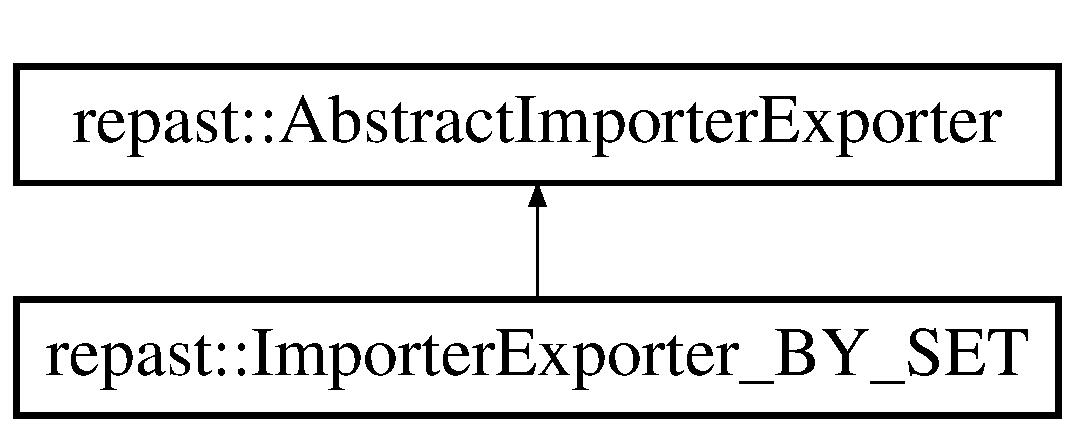
\includegraphics[height=2.000000cm]{classrepast_1_1_importer_exporter___b_y___s_e_t}
\end{center}
\end{figure}
\subsection*{Public Member Functions}
\begin{DoxyCompactItemize}
\item 
\hypertarget{classrepast_1_1_importer_exporter___b_y___s_e_t_aecb47913ae4c330551286d972a8ac4ad}{virtual const std\-::set$<$ int $>$ \& {\bfseries get\-Exporting\-Processes} ()}\label{classrepast_1_1_importer_exporter___b_y___s_e_t_aecb47913ae4c330551286d972a8ac4ad}

\item 
\hypertarget{classrepast_1_1_importer_exporter___b_y___s_e_t_ae083fd746ee19bd910f53772fd946702}{const std\-::set$<$ int $>$ \& {\bfseries get\-Exporting\-Processes} (std\-::string set\-Name)}\label{classrepast_1_1_importer_exporter___b_y___s_e_t_ae083fd746ee19bd910f53772fd946702}

\item 
\hypertarget{classrepast_1_1_importer_exporter___b_y___s_e_t_aba0ac96cc448d3393ea83a82ce4ce9ca}{virtual void {\bfseries register\-Outgoing\-Requests} (\hyperlink{classrepast_1_1_agent_request}{Agent\-Request} \&request)}\label{classrepast_1_1_importer_exporter___b_y___s_e_t_aba0ac96cc448d3393ea83a82ce4ce9ca}

\item 
\hypertarget{classrepast_1_1_importer_exporter___b_y___s_e_t_a93fd8bbbdebf03d145ede0af6b80c07d}{void {\bfseries register\-Outgoing\-Requests} (\hyperlink{classrepast_1_1_agent_request}{Agent\-Request} \&request, std\-::string set\-Name, A\-G\-E\-N\-T\-\_\-\-I\-M\-P\-O\-R\-T\-E\-R\-\_\-\-E\-X\-P\-O\-R\-T\-E\-R\-\_\-\-T\-Y\-P\-E set\-Type=D\-E\-F\-A\-U\-L\-T\-\_\-\-E\-N\-U\-M\-\_\-\-S\-Y\-M\-B\-O\-L)}\label{classrepast_1_1_importer_exporter___b_y___s_e_t_a93fd8bbbdebf03d145ede0af6b80c07d}

\item 
\hypertarget{classrepast_1_1_importer_exporter___b_y___s_e_t_a669356de5e51cd3e2225521ee234d9e9}{virtual void {\bfseries imported\-Agent\-Is\-Removed} (const \hyperlink{classrepast_1_1_agent_id}{Agent\-Id} \&id)}\label{classrepast_1_1_importer_exporter___b_y___s_e_t_a669356de5e51cd3e2225521ee234d9e9}

\item 
\hypertarget{classrepast_1_1_importer_exporter___b_y___s_e_t_a2a72cb02534f10f9da5a913d1cd09a85}{virtual void {\bfseries imported\-Agent\-Is\-Moved} (const \hyperlink{classrepast_1_1_agent_id}{Agent\-Id} \&id, int new\-Process)}\label{classrepast_1_1_importer_exporter___b_y___s_e_t_a2a72cb02534f10f9da5a913d1cd09a85}

\item 
\hypertarget{classrepast_1_1_importer_exporter___b_y___s_e_t_a84b98ad04ccb7ce97184377074995644}{virtual void {\bfseries imported\-Agent\-Is\-Now\-Local} (const \hyperlink{classrepast_1_1_agent_id}{Agent\-Id} \&id)}\label{classrepast_1_1_importer_exporter___b_y___s_e_t_a84b98ad04ccb7ce97184377074995644}

\item 
\hypertarget{classrepast_1_1_importer_exporter___b_y___s_e_t_ad44c849f9ffb2832a18cbc2c68ad6999}{virtual const \\*
Abstract\-Exporter\-::\-Status\-Map $\ast$ {\bfseries get\-Outgoing\-Status\-Changes} ()}\label{classrepast_1_1_importer_exporter___b_y___s_e_t_ad44c849f9ffb2832a18cbc2c68ad6999}

\item 
\hypertarget{classrepast_1_1_importer_exporter___b_y___s_e_t_af4e397c2d5ff57899c68dc2d5d8259cb}{virtual const std\-::set$<$ int $>$ \& {\bfseries get\-Processes\-Exported\-To} ()}\label{classrepast_1_1_importer_exporter___b_y___s_e_t_af4e397c2d5ff57899c68dc2d5d8259cb}

\item 
\hypertarget{classrepast_1_1_importer_exporter___b_y___s_e_t_a578132700de4662efb239677c9c335bb}{const std\-::set$<$ int $>$ \& {\bfseries get\-Processes\-Exported\-To} (std\-::string set\-Name)}\label{classrepast_1_1_importer_exporter___b_y___s_e_t_a578132700de4662efb239677c9c335bb}

\item 
\hypertarget{classrepast_1_1_importer_exporter___b_y___s_e_t_ae7de9ae6a65eeb2c156bba1a1add61d6}{virtual void {\bfseries register\-Incoming\-Requests} (std\-::vector$<$ \hyperlink{classrepast_1_1_agent_request}{Agent\-Request} $>$ \&requests)}\label{classrepast_1_1_importer_exporter___b_y___s_e_t_ae7de9ae6a65eeb2c156bba1a1add61d6}

\item 
\hypertarget{classrepast_1_1_importer_exporter___b_y___s_e_t_afc2f89de3a127c49597e1abc8f84c77e}{void {\bfseries register\-Incoming\-Requests} (std\-::vector$<$ \hyperlink{classrepast_1_1_agent_request}{Agent\-Request} $>$ \&requests, std\-::string set\-Name)}\label{classrepast_1_1_importer_exporter___b_y___s_e_t_afc2f89de3a127c49597e1abc8f84c77e}

\item 
\hypertarget{classrepast_1_1_importer_exporter___b_y___s_e_t_ab451be52b3ce98e129fe07d064c8f1d0}{virtual void {\bfseries agent\-Removed} (const \hyperlink{classrepast_1_1_agent_id}{Agent\-Id} \&id)}\label{classrepast_1_1_importer_exporter___b_y___s_e_t_ab451be52b3ce98e129fe07d064c8f1d0}

\item 
\hypertarget{classrepast_1_1_importer_exporter___b_y___s_e_t_a0c56fa3b5c3d45b2c641419052182da0}{virtual void {\bfseries agent\-Moved} (const \hyperlink{classrepast_1_1_agent_id}{Agent\-Id} \&id, int new\-Process)}\label{classrepast_1_1_importer_exporter___b_y___s_e_t_a0c56fa3b5c3d45b2c641419052182da0}

\item 
\hypertarget{classrepast_1_1_importer_exporter___b_y___s_e_t_a45f53a2b8cbed32a994ef44fcb707728}{virtual void {\bfseries incorporate\-Agent\-Exporter\-Info} (std\-::map$<$ int, \hyperlink{classrepast_1_1_agent_request}{Agent\-Request} $\ast$ $>$ info)}\label{classrepast_1_1_importer_exporter___b_y___s_e_t_a45f53a2b8cbed32a994ef44fcb707728}

\item 
\hypertarget{classrepast_1_1_importer_exporter___b_y___s_e_t_abab0db9ba254d5ea5fe0db6b87a7d3d7}{void {\bfseries incorporate\-Agent\-Exporter\-Info} (std\-::map$<$ std\-::string, std\-::map$<$ int, \hyperlink{classrepast_1_1_agent_request}{Agent\-Request} $\ast$ $>$ $\ast$ $>$ info)}\label{classrepast_1_1_importer_exporter___b_y___s_e_t_abab0db9ba254d5ea5fe0db6b87a7d3d7}

\item 
\hypertarget{classrepast_1_1_importer_exporter___b_y___s_e_t_ab07661092d59b852fba56e10fa5b49d7}{virtual void {\bfseries clear\-Status\-Map} ()}\label{classrepast_1_1_importer_exporter___b_y___s_e_t_ab07661092d59b852fba56e10fa5b49d7}

\item 
\hypertarget{classrepast_1_1_importer_exporter___b_y___s_e_t_a9ba508377a9cd6b8a5f70c0634fd086c}{virtual Agent\-Exporter\-Info $\ast$ {\bfseries get\-Agent\-Export\-Info} (int dest\-Proc)}\label{classrepast_1_1_importer_exporter___b_y___s_e_t_a9ba508377a9cd6b8a5f70c0634fd086c}

\item 
\hypertarget{classrepast_1_1_importer_exporter___b_y___s_e_t_ad6d9611812f2b0872152126bff36f8cf}{virtual void {\bfseries clear\-Agent\-Export\-Info} ()}\label{classrepast_1_1_importer_exporter___b_y___s_e_t_ad6d9611812f2b0872152126bff36f8cf}

\item 
\hypertarget{classrepast_1_1_importer_exporter___b_y___s_e_t_a49fdc6cf040166d79cd75a06c8a9f77c}{virtual const std\-::map$<$ int, \\*
\hyperlink{classrepast_1_1_agent_request}{Agent\-Request} $>$ \& {\bfseries get\-Agents\-To\-Export} ()}\label{classrepast_1_1_importer_exporter___b_y___s_e_t_a49fdc6cf040166d79cd75a06c8a9f77c}

\item 
\hypertarget{classrepast_1_1_importer_exporter___b_y___s_e_t_a47875477bcfa1417bd94c500708ca8ac}{const std\-::map$<$ int, \\*
\hyperlink{classrepast_1_1_agent_request}{Agent\-Request} $>$ \& {\bfseries get\-Agents\-To\-Export} (std\-::string set\-Name)}\label{classrepast_1_1_importer_exporter___b_y___s_e_t_a47875477bcfa1417bd94c500708ca8ac}

\item 
virtual std\-::string \hyperlink{classrepast_1_1_importer_exporter___b_y___s_e_t_a440dc78901d8811ba6046d769df298d9}{version} ()
\begin{DoxyCompactList}\small\item\em Returns the version of this \hyperlink{classrepast_1_1_abstract_importer_exporter}{Abstract\-Importer\-Exporter}. \end{DoxyCompactList}\item 
\hypertarget{classrepast_1_1_importer_exporter___b_y___s_e_t_ab1c9657eb2842f25530dbb5dc932739c}{void {\bfseries drop\-Set} (std\-::string set\-Name)}\label{classrepast_1_1_importer_exporter___b_y___s_e_t_ab1c9657eb2842f25530dbb5dc932739c}

\item 
\hypertarget{classrepast_1_1_importer_exporter___b_y___s_e_t_a02c13955439cefc10f024f36c5d0a74f}{virtual std\-::string \hyperlink{classrepast_1_1_importer_exporter___b_y___s_e_t_a02c13955439cefc10f024f36c5d0a74f}{get\-Report} ()}\label{classrepast_1_1_importer_exporter___b_y___s_e_t_a02c13955439cefc10f024f36c5d0a74f}

\begin{DoxyCompactList}\small\item\em Gets a printable report of the state of this object. \end{DoxyCompactList}\item 
\hypertarget{classrepast_1_1_importer_exporter___b_y___s_e_t_a8037129cdc08cbbea56c4a680afa1059}{virtual void {\bfseries get\-Set\-Of\-Agents\-Being\-Imported} (std\-::set$<$ \hyperlink{classrepast_1_1_agent_id}{Agent\-Id} $>$ \&set)}\label{classrepast_1_1_importer_exporter___b_y___s_e_t_a8037129cdc08cbbea56c4a680afa1059}

\item 
\hypertarget{classrepast_1_1_importer_exporter___b_y___s_e_t_a586fb335673c8a4ec6f9fd9852b209a8}{void {\bfseries get\-Set\-Of\-Agents\-Being\-Imported} (std\-::set$<$ \hyperlink{classrepast_1_1_agent_id}{Agent\-Id} $>$ \&set, std\-::string exclude\-Set)}\label{classrepast_1_1_importer_exporter___b_y___s_e_t_a586fb335673c8a4ec6f9fd9852b209a8}

\item 
\hypertarget{classrepast_1_1_importer_exporter___b_y___s_e_t_a3e197efc21efc60432241fbf60097fe9}{virtual void {\bfseries clear} ()}\label{classrepast_1_1_importer_exporter___b_y___s_e_t_a3e197efc21efc60432241fbf60097fe9}

\item 
\hypertarget{classrepast_1_1_importer_exporter___b_y___s_e_t_afdea331d16b4b0f6ef4083cbb33b34dc}{void {\bfseries clear} (std\-::string set\-Name)}\label{classrepast_1_1_importer_exporter___b_y___s_e_t_afdea331d16b4b0f6ef4083cbb33b34dc}

\item 
\hypertarget{classrepast_1_1_importer_exporter___b_y___s_e_t_ae6f7f705ff22c4675eccb8ba2730c753}{virtual void {\bfseries clear\-Exporter} ()}\label{classrepast_1_1_importer_exporter___b_y___s_e_t_ae6f7f705ff22c4675eccb8ba2730c753}

\item 
\hypertarget{classrepast_1_1_importer_exporter___b_y___s_e_t_a2bdbb566faa85117e101492a58e82f6d}{void {\bfseries clear\-Exporter} (std\-::string set\-Name)}\label{classrepast_1_1_importer_exporter___b_y___s_e_t_a2bdbb566faa85117e101492a58e82f6d}

\item 
\hypertarget{classrepast_1_1_importer_exporter___b_y___s_e_t_a099e4e82ac21783ec8740a84f1df44a9}{void {\bfseries clear\-Export\-To\-Specific\-Proc} (int rank)}\label{classrepast_1_1_importer_exporter___b_y___s_e_t_a099e4e82ac21783ec8740a84f1df44a9}

\end{DoxyCompactItemize}
\subsection*{Additional Inherited Members}


\subsection{Detailed Description}
Implementation of the \hyperlink{classrepast_1_1_abstract_importer_exporter}{Abstract\-Importer\-Exporter} class that wraps a collection of \hyperlink{classrepast_1_1_abstract_importer_exporter}{Abstract\-Importer\-Exporter} objects that can be referenced by name. 

Each object can contain a different collection of agents, which were requested with an associated name for the importer/exporter to be used. They can then be updated separately, allowing for improved performance under certain circumstances. 

\subsection{Member Function Documentation}
\hypertarget{classrepast_1_1_importer_exporter___b_y___s_e_t_a440dc78901d8811ba6046d769df298d9}{\index{repast\-::\-Importer\-Exporter\-\_\-\-B\-Y\-\_\-\-S\-E\-T@{repast\-::\-Importer\-Exporter\-\_\-\-B\-Y\-\_\-\-S\-E\-T}!version@{version}}
\index{version@{version}!repast::ImporterExporter_BY_SET@{repast\-::\-Importer\-Exporter\-\_\-\-B\-Y\-\_\-\-S\-E\-T}}
\subsubsection[{version}]{\setlength{\rightskip}{0pt plus 5cm}std\-::string Importer\-Exporter\-\_\-\-B\-Y\-\_\-\-S\-E\-T\-::version (
\begin{DoxyParamCaption}
{}
\end{DoxyParamCaption}
)\hspace{0.3cm}{\ttfamily [virtual]}}}\label{classrepast_1_1_importer_exporter___b_y___s_e_t_a440dc78901d8811ba6046d769df298d9}


Returns the version of this \hyperlink{classrepast_1_1_abstract_importer_exporter}{Abstract\-Importer\-Exporter}. 

The version is a string that indicates the semantic version of the importer and the exporter (e.\-g. \char`\"{}\-C\-O\-U\-N\-T\-\_\-\-L\-I\-S\-T\char`\"{}) 

Implements \hyperlink{classrepast_1_1_abstract_importer_exporter_a27a52b5ec4ec41e3ed6bf1c8819c25fc}{repast\-::\-Abstract\-Importer\-Exporter}.



The documentation for this class was generated from the following files\-:\begin{DoxyCompactItemize}
\item 
repast\-\_\-hpc/Agent\-Importer\-Exporter.\-h\item 
repast\-\_\-hpc/Agent\-Importer\-Exporter.\-cpp\end{DoxyCompactItemize}

\hypertarget{classrepast_1_1_importer_exporter___c_o_u_n_t___l_i_s_t}{\section{repast\-:\-:Importer\-Exporter\-\_\-\-C\-O\-U\-N\-T\-\_\-\-L\-I\-S\-T Class Reference}
\label{classrepast_1_1_importer_exporter___c_o_u_n_t___l_i_s_t}\index{repast\-::\-Importer\-Exporter\-\_\-\-C\-O\-U\-N\-T\-\_\-\-L\-I\-S\-T@{repast\-::\-Importer\-Exporter\-\_\-\-C\-O\-U\-N\-T\-\_\-\-L\-I\-S\-T}}
}


An implementation of \hyperlink{classrepast_1_1_abstract_importer_exporter}{Abstract\-Importer\-Exporter} that uses an importer of type '\hyperlink{classrepast_1_1_importer___c_o_u_n_t}{Importer\-\_\-\-C\-O\-U\-N\-T}' and an exporter of type '\hyperlink{classrepast_1_1_exporter___l_i_s_t}{Exporter\-\_\-\-L\-I\-S\-T}'.  




{\ttfamily \#include $<$Agent\-Importer\-Exporter.\-h$>$}

Inheritance diagram for repast\-:\-:Importer\-Exporter\-\_\-\-C\-O\-U\-N\-T\-\_\-\-L\-I\-S\-T\-:\begin{figure}[H]
\begin{center}
\leavevmode
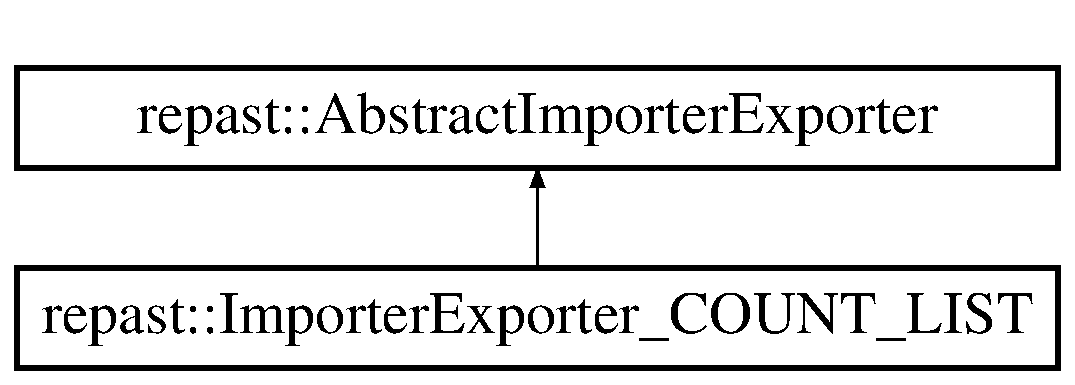
\includegraphics[height=2.000000cm]{classrepast_1_1_importer_exporter___c_o_u_n_t___l_i_s_t}
\end{center}
\end{figure}
\subsection*{Public Member Functions}
\begin{DoxyCompactItemize}
\item 
\hypertarget{classrepast_1_1_importer_exporter___c_o_u_n_t___l_i_s_t_acd154e0d330e2313430184323f384576}{{\bfseries Importer\-Exporter\-\_\-\-C\-O\-U\-N\-T\-\_\-\-L\-I\-S\-T} (Abstract\-Exporter\-::\-Status\-Map $\ast$outgoing\-Status\-Map, \hyperlink{classrepast_1_1_agent_exporter_data}{Agent\-Exporter\-Data} $\ast$outgoing\-Agent\-Exporter\-Info)}\label{classrepast_1_1_importer_exporter___c_o_u_n_t___l_i_s_t_acd154e0d330e2313430184323f384576}

\item 
virtual std\-::string \hyperlink{classrepast_1_1_importer_exporter___c_o_u_n_t___l_i_s_t_a576d3dc96aa00bab8a4f0bbe6e64981c}{version} ()
\begin{DoxyCompactList}\small\item\em Returns the version of this \hyperlink{classrepast_1_1_abstract_importer_exporter}{Abstract\-Importer\-Exporter}. \end{DoxyCompactList}\end{DoxyCompactItemize}
\subsection*{Additional Inherited Members}


\subsection{Detailed Description}
An implementation of \hyperlink{classrepast_1_1_abstract_importer_exporter}{Abstract\-Importer\-Exporter} that uses an importer of type '\hyperlink{classrepast_1_1_importer___c_o_u_n_t}{Importer\-\_\-\-C\-O\-U\-N\-T}' and an exporter of type '\hyperlink{classrepast_1_1_exporter___l_i_s_t}{Exporter\-\_\-\-L\-I\-S\-T}'. 

\subsection{Member Function Documentation}
\hypertarget{classrepast_1_1_importer_exporter___c_o_u_n_t___l_i_s_t_a576d3dc96aa00bab8a4f0bbe6e64981c}{\index{repast\-::\-Importer\-Exporter\-\_\-\-C\-O\-U\-N\-T\-\_\-\-L\-I\-S\-T@{repast\-::\-Importer\-Exporter\-\_\-\-C\-O\-U\-N\-T\-\_\-\-L\-I\-S\-T}!version@{version}}
\index{version@{version}!repast::ImporterExporter_COUNT_LIST@{repast\-::\-Importer\-Exporter\-\_\-\-C\-O\-U\-N\-T\-\_\-\-L\-I\-S\-T}}
\subsubsection[{version}]{\setlength{\rightskip}{0pt plus 5cm}std\-::string Importer\-Exporter\-\_\-\-C\-O\-U\-N\-T\-\_\-\-L\-I\-S\-T\-::version (
\begin{DoxyParamCaption}
{}
\end{DoxyParamCaption}
)\hspace{0.3cm}{\ttfamily [virtual]}}}\label{classrepast_1_1_importer_exporter___c_o_u_n_t___l_i_s_t_a576d3dc96aa00bab8a4f0bbe6e64981c}


Returns the version of this \hyperlink{classrepast_1_1_abstract_importer_exporter}{Abstract\-Importer\-Exporter}. 

The version is a string that indicates the semantic version of the importer and the exporter (e.\-g. \char`\"{}\-C\-O\-U\-N\-T\-\_\-\-L\-I\-S\-T\char`\"{}) 

Implements \hyperlink{classrepast_1_1_abstract_importer_exporter_a27a52b5ec4ec41e3ed6bf1c8819c25fc}{repast\-::\-Abstract\-Importer\-Exporter}.



The documentation for this class was generated from the following files\-:\begin{DoxyCompactItemize}
\item 
repast\-\_\-hpc/Agent\-Importer\-Exporter.\-h\item 
repast\-\_\-hpc/Agent\-Importer\-Exporter.\-cpp\end{DoxyCompactItemize}

\hypertarget{classrepast_1_1_importer_exporter___c_o_u_n_t___s_e_t}{\section{repast\-:\-:Importer\-Exporter\-\_\-\-C\-O\-U\-N\-T\-\_\-\-S\-E\-T Class Reference}
\label{classrepast_1_1_importer_exporter___c_o_u_n_t___s_e_t}\index{repast\-::\-Importer\-Exporter\-\_\-\-C\-O\-U\-N\-T\-\_\-\-S\-E\-T@{repast\-::\-Importer\-Exporter\-\_\-\-C\-O\-U\-N\-T\-\_\-\-S\-E\-T}}
}


An implementation of \hyperlink{classrepast_1_1_abstract_importer_exporter}{Abstract\-Importer\-Exporter} that uses an importer of type '\hyperlink{classrepast_1_1_importer___c_o_u_n_t}{Importer\-\_\-\-C\-O\-U\-N\-T}' and an exporter of type '\hyperlink{classrepast_1_1_exporter___s_e_t}{Exporter\-\_\-\-S\-E\-T}'.  




{\ttfamily \#include $<$Agent\-Importer\-Exporter.\-h$>$}

Inheritance diagram for repast\-:\-:Importer\-Exporter\-\_\-\-C\-O\-U\-N\-T\-\_\-\-S\-E\-T\-:\begin{figure}[H]
\begin{center}
\leavevmode
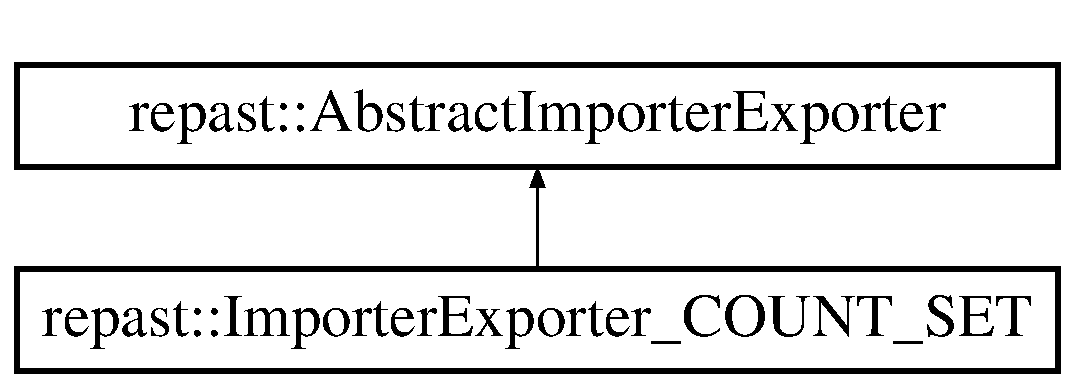
\includegraphics[height=2.000000cm]{classrepast_1_1_importer_exporter___c_o_u_n_t___s_e_t}
\end{center}
\end{figure}
\subsection*{Public Member Functions}
\begin{DoxyCompactItemize}
\item 
\hypertarget{classrepast_1_1_importer_exporter___c_o_u_n_t___s_e_t_a03c9be6ac0338a286aad918f8ee7ca1e}{{\bfseries Importer\-Exporter\-\_\-\-C\-O\-U\-N\-T\-\_\-\-S\-E\-T} (Abstract\-Exporter\-::\-Status\-Map $\ast$outgoing\-Status\-Map, \hyperlink{classrepast_1_1_agent_exporter_data}{Agent\-Exporter\-Data} $\ast$outgoing\-Agent\-Exporter\-Info)}\label{classrepast_1_1_importer_exporter___c_o_u_n_t___s_e_t_a03c9be6ac0338a286aad918f8ee7ca1e}

\item 
virtual std\-::string \hyperlink{classrepast_1_1_importer_exporter___c_o_u_n_t___s_e_t_a4feec2dc77e01798f1331381198ce3e7}{version} ()
\begin{DoxyCompactList}\small\item\em Returns the version of this \hyperlink{classrepast_1_1_abstract_importer_exporter}{Abstract\-Importer\-Exporter}. \end{DoxyCompactList}\end{DoxyCompactItemize}
\subsection*{Additional Inherited Members}


\subsection{Detailed Description}
An implementation of \hyperlink{classrepast_1_1_abstract_importer_exporter}{Abstract\-Importer\-Exporter} that uses an importer of type '\hyperlink{classrepast_1_1_importer___c_o_u_n_t}{Importer\-\_\-\-C\-O\-U\-N\-T}' and an exporter of type '\hyperlink{classrepast_1_1_exporter___s_e_t}{Exporter\-\_\-\-S\-E\-T}'. 

\subsection{Member Function Documentation}
\hypertarget{classrepast_1_1_importer_exporter___c_o_u_n_t___s_e_t_a4feec2dc77e01798f1331381198ce3e7}{\index{repast\-::\-Importer\-Exporter\-\_\-\-C\-O\-U\-N\-T\-\_\-\-S\-E\-T@{repast\-::\-Importer\-Exporter\-\_\-\-C\-O\-U\-N\-T\-\_\-\-S\-E\-T}!version@{version}}
\index{version@{version}!repast::ImporterExporter_COUNT_SET@{repast\-::\-Importer\-Exporter\-\_\-\-C\-O\-U\-N\-T\-\_\-\-S\-E\-T}}
\subsubsection[{version}]{\setlength{\rightskip}{0pt plus 5cm}std\-::string Importer\-Exporter\-\_\-\-C\-O\-U\-N\-T\-\_\-\-S\-E\-T\-::version (
\begin{DoxyParamCaption}
{}
\end{DoxyParamCaption}
)\hspace{0.3cm}{\ttfamily [virtual]}}}\label{classrepast_1_1_importer_exporter___c_o_u_n_t___s_e_t_a4feec2dc77e01798f1331381198ce3e7}


Returns the version of this \hyperlink{classrepast_1_1_abstract_importer_exporter}{Abstract\-Importer\-Exporter}. 

The version is a string that indicates the semantic version of the importer and the exporter (e.\-g. \char`\"{}\-C\-O\-U\-N\-T\-\_\-\-L\-I\-S\-T\char`\"{}) 

Implements \hyperlink{classrepast_1_1_abstract_importer_exporter_a27a52b5ec4ec41e3ed6bf1c8819c25fc}{repast\-::\-Abstract\-Importer\-Exporter}.



The documentation for this class was generated from the following files\-:\begin{DoxyCompactItemize}
\item 
repast\-\_\-hpc/Agent\-Importer\-Exporter.\-h\item 
repast\-\_\-hpc/Agent\-Importer\-Exporter.\-cpp\end{DoxyCompactItemize}

\hypertarget{classrepast_1_1_importer_exporter___l_i_s_t}{\section{repast\-:\-:Importer\-Exporter\-\_\-\-L\-I\-S\-T Class Reference}
\label{classrepast_1_1_importer_exporter___l_i_s_t}\index{repast\-::\-Importer\-Exporter\-\_\-\-L\-I\-S\-T@{repast\-::\-Importer\-Exporter\-\_\-\-L\-I\-S\-T}}
}


An implementation of \hyperlink{classrepast_1_1_abstract_importer_exporter}{Abstract\-Importer\-Exporter} that uses an importer of type '\hyperlink{classrepast_1_1_importer___l_i_s_t}{Importer\-\_\-\-L\-I\-S\-T}' and an exporter of type '\hyperlink{classrepast_1_1_exporter___l_i_s_t}{Exporter\-\_\-\-L\-I\-S\-T}'.  




{\ttfamily \#include $<$Agent\-Importer\-Exporter.\-h$>$}

Inheritance diagram for repast\-:\-:Importer\-Exporter\-\_\-\-L\-I\-S\-T\-:\begin{figure}[H]
\begin{center}
\leavevmode
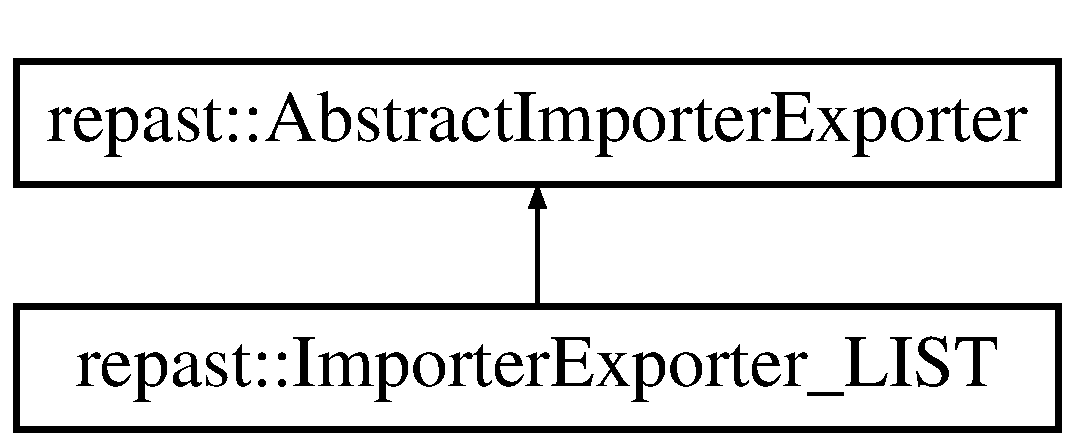
\includegraphics[height=2.000000cm]{classrepast_1_1_importer_exporter___l_i_s_t}
\end{center}
\end{figure}
\subsection*{Public Member Functions}
\begin{DoxyCompactItemize}
\item 
\hypertarget{classrepast_1_1_importer_exporter___l_i_s_t_abefea36aba632900932b731688615724}{{\bfseries Importer\-Exporter\-\_\-\-L\-I\-S\-T} (Abstract\-Exporter\-::\-Status\-Map $\ast$outgoing\-Status\-Map, \hyperlink{classrepast_1_1_agent_exporter_data}{Agent\-Exporter\-Data} $\ast$outgoing\-Agent\-Exporter\-Info)}\label{classrepast_1_1_importer_exporter___l_i_s_t_abefea36aba632900932b731688615724}

\item 
virtual std\-::string \hyperlink{classrepast_1_1_importer_exporter___l_i_s_t_a548c16411acb6e380e9e27139148e294}{version} ()
\begin{DoxyCompactList}\small\item\em Returns the version of this \hyperlink{classrepast_1_1_abstract_importer_exporter}{Abstract\-Importer\-Exporter}. \end{DoxyCompactList}\end{DoxyCompactItemize}
\subsection*{Additional Inherited Members}


\subsection{Detailed Description}
An implementation of \hyperlink{classrepast_1_1_abstract_importer_exporter}{Abstract\-Importer\-Exporter} that uses an importer of type '\hyperlink{classrepast_1_1_importer___l_i_s_t}{Importer\-\_\-\-L\-I\-S\-T}' and an exporter of type '\hyperlink{classrepast_1_1_exporter___l_i_s_t}{Exporter\-\_\-\-L\-I\-S\-T}'. 

\subsection{Member Function Documentation}
\hypertarget{classrepast_1_1_importer_exporter___l_i_s_t_a548c16411acb6e380e9e27139148e294}{\index{repast\-::\-Importer\-Exporter\-\_\-\-L\-I\-S\-T@{repast\-::\-Importer\-Exporter\-\_\-\-L\-I\-S\-T}!version@{version}}
\index{version@{version}!repast::ImporterExporter_LIST@{repast\-::\-Importer\-Exporter\-\_\-\-L\-I\-S\-T}}
\subsubsection[{version}]{\setlength{\rightskip}{0pt plus 5cm}std\-::string Importer\-Exporter\-\_\-\-L\-I\-S\-T\-::version (
\begin{DoxyParamCaption}
{}
\end{DoxyParamCaption}
)\hspace{0.3cm}{\ttfamily [virtual]}}}\label{classrepast_1_1_importer_exporter___l_i_s_t_a548c16411acb6e380e9e27139148e294}


Returns the version of this \hyperlink{classrepast_1_1_abstract_importer_exporter}{Abstract\-Importer\-Exporter}. 

The version is a string that indicates the semantic version of the importer and the exporter (e.\-g. \char`\"{}\-C\-O\-U\-N\-T\-\_\-\-L\-I\-S\-T\char`\"{}) 

Implements \hyperlink{classrepast_1_1_abstract_importer_exporter_a27a52b5ec4ec41e3ed6bf1c8819c25fc}{repast\-::\-Abstract\-Importer\-Exporter}.



The documentation for this class was generated from the following files\-:\begin{DoxyCompactItemize}
\item 
repast\-\_\-hpc/Agent\-Importer\-Exporter.\-h\item 
repast\-\_\-hpc/Agent\-Importer\-Exporter.\-cpp\end{DoxyCompactItemize}

\hypertarget{classrepast_1_1_importer_exporter___m_a_p__int}{\section{repast\-:\-:Importer\-Exporter\-\_\-\-M\-A\-P\-\_\-int Class Reference}
\label{classrepast_1_1_importer_exporter___m_a_p__int}\index{repast\-::\-Importer\-Exporter\-\_\-\-M\-A\-P\-\_\-int@{repast\-::\-Importer\-Exporter\-\_\-\-M\-A\-P\-\_\-int}}
}


An implementation of \hyperlink{classrepast_1_1_abstract_importer_exporter}{Abstract\-Importer\-Exporter} that uses an importer of type '\hyperlink{classrepast_1_1_importer___m_a_p__int}{Importer\-\_\-\-M\-A\-P\-\_\-int}' and an exporter of type '\hyperlink{classrepast_1_1_exporter___l_i_s_t}{Exporter\-\_\-\-L\-I\-S\-T}'.  




{\ttfamily \#include $<$Agent\-Importer\-Exporter.\-h$>$}

Inheritance diagram for repast\-:\-:Importer\-Exporter\-\_\-\-M\-A\-P\-\_\-int\-:\begin{figure}[H]
\begin{center}
\leavevmode
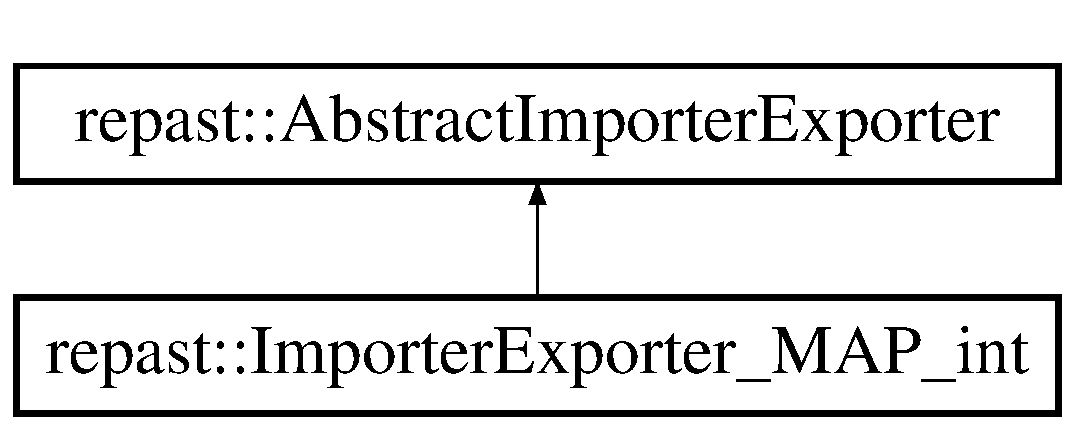
\includegraphics[height=2.000000cm]{classrepast_1_1_importer_exporter___m_a_p__int}
\end{center}
\end{figure}
\subsection*{Public Member Functions}
\begin{DoxyCompactItemize}
\item 
\hypertarget{classrepast_1_1_importer_exporter___m_a_p__int_a39fcbc169fddfb9c52b8b2cb80d3c4c9}{{\bfseries Importer\-Exporter\-\_\-\-M\-A\-P\-\_\-int} (Abstract\-Exporter\-::\-Status\-Map $\ast$outgoing\-Status\-Map, \hyperlink{classrepast_1_1_agent_exporter_data}{Agent\-Exporter\-Data} $\ast$outgoing\-Agent\-Exporter\-Info)}\label{classrepast_1_1_importer_exporter___m_a_p__int_a39fcbc169fddfb9c52b8b2cb80d3c4c9}

\item 
virtual std\-::string \hyperlink{classrepast_1_1_importer_exporter___m_a_p__int_a801fce0ea8f65aa5b23cc9b1cc9dd818}{version} ()
\begin{DoxyCompactList}\small\item\em Returns the version of this \hyperlink{classrepast_1_1_abstract_importer_exporter}{Abstract\-Importer\-Exporter}. \end{DoxyCompactList}\end{DoxyCompactItemize}
\subsection*{Additional Inherited Members}


\subsection{Detailed Description}
An implementation of \hyperlink{classrepast_1_1_abstract_importer_exporter}{Abstract\-Importer\-Exporter} that uses an importer of type '\hyperlink{classrepast_1_1_importer___m_a_p__int}{Importer\-\_\-\-M\-A\-P\-\_\-int}' and an exporter of type '\hyperlink{classrepast_1_1_exporter___l_i_s_t}{Exporter\-\_\-\-L\-I\-S\-T}'. 

\subsection{Member Function Documentation}
\hypertarget{classrepast_1_1_importer_exporter___m_a_p__int_a801fce0ea8f65aa5b23cc9b1cc9dd818}{\index{repast\-::\-Importer\-Exporter\-\_\-\-M\-A\-P\-\_\-int@{repast\-::\-Importer\-Exporter\-\_\-\-M\-A\-P\-\_\-int}!version@{version}}
\index{version@{version}!repast::ImporterExporter_MAP_int@{repast\-::\-Importer\-Exporter\-\_\-\-M\-A\-P\-\_\-int}}
\subsubsection[{version}]{\setlength{\rightskip}{0pt plus 5cm}std\-::string Importer\-Exporter\-\_\-\-M\-A\-P\-\_\-int\-::version (
\begin{DoxyParamCaption}
{}
\end{DoxyParamCaption}
)\hspace{0.3cm}{\ttfamily [virtual]}}}\label{classrepast_1_1_importer_exporter___m_a_p__int_a801fce0ea8f65aa5b23cc9b1cc9dd818}


Returns the version of this \hyperlink{classrepast_1_1_abstract_importer_exporter}{Abstract\-Importer\-Exporter}. 

The version is a string that indicates the semantic version of the importer and the exporter (e.\-g. \char`\"{}\-C\-O\-U\-N\-T\-\_\-\-L\-I\-S\-T\char`\"{}) 

Implements \hyperlink{classrepast_1_1_abstract_importer_exporter_a27a52b5ec4ec41e3ed6bf1c8819c25fc}{repast\-::\-Abstract\-Importer\-Exporter}.



The documentation for this class was generated from the following files\-:\begin{DoxyCompactItemize}
\item 
repast\-\_\-hpc/Agent\-Importer\-Exporter.\-h\item 
repast\-\_\-hpc/Agent\-Importer\-Exporter.\-cpp\end{DoxyCompactItemize}

\hypertarget{classrepast_1_1_importer_exporter___s_e_t}{\section{repast\-:\-:Importer\-Exporter\-\_\-\-S\-E\-T Class Reference}
\label{classrepast_1_1_importer_exporter___s_e_t}\index{repast\-::\-Importer\-Exporter\-\_\-\-S\-E\-T@{repast\-::\-Importer\-Exporter\-\_\-\-S\-E\-T}}
}


An implementation of \hyperlink{classrepast_1_1_abstract_importer_exporter}{Abstract\-Importer\-Exporter} that uses an importer of type '\hyperlink{classrepast_1_1_importer___s_e_t}{Importer\-\_\-\-S\-E\-T}' and an exporter of type '\hyperlink{classrepast_1_1_exporter___l_i_s_t}{Exporter\-\_\-\-L\-I\-S\-T}'.  




{\ttfamily \#include $<$Agent\-Importer\-Exporter.\-h$>$}

Inheritance diagram for repast\-:\-:Importer\-Exporter\-\_\-\-S\-E\-T\-:\begin{figure}[H]
\begin{center}
\leavevmode
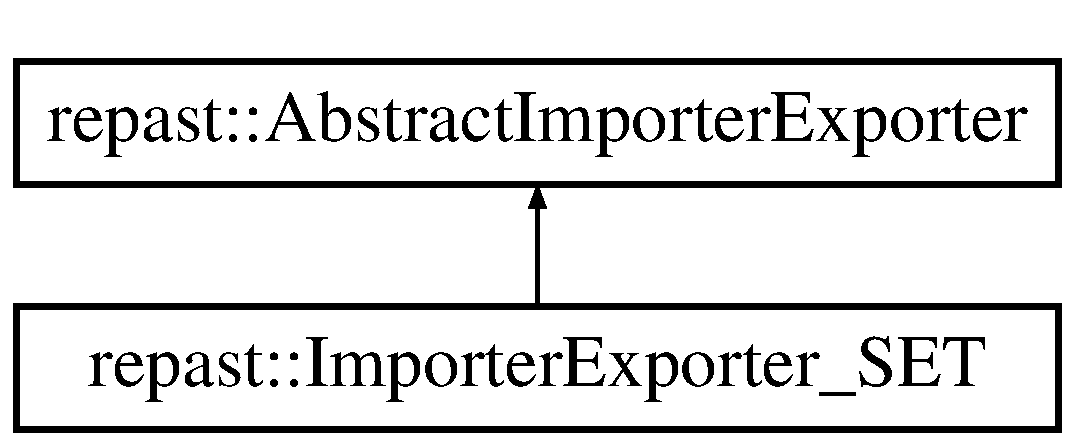
\includegraphics[height=2.000000cm]{classrepast_1_1_importer_exporter___s_e_t}
\end{center}
\end{figure}
\subsection*{Public Member Functions}
\begin{DoxyCompactItemize}
\item 
\hypertarget{classrepast_1_1_importer_exporter___s_e_t_a3cec27920ea93f83477f5b6a0aaf2c36}{{\bfseries Importer\-Exporter\-\_\-\-S\-E\-T} (Abstract\-Exporter\-::\-Status\-Map $\ast$outgoing\-Status\-Map, \hyperlink{classrepast_1_1_agent_exporter_data}{Agent\-Exporter\-Data} $\ast$outgoing\-Agent\-Exporter\-Info)}\label{classrepast_1_1_importer_exporter___s_e_t_a3cec27920ea93f83477f5b6a0aaf2c36}

\item 
virtual std\-::string \hyperlink{classrepast_1_1_importer_exporter___s_e_t_a94bcc5a0cb77c6550927663b04410ca2}{version} ()
\begin{DoxyCompactList}\small\item\em Returns the version of this \hyperlink{classrepast_1_1_abstract_importer_exporter}{Abstract\-Importer\-Exporter}. \end{DoxyCompactList}\end{DoxyCompactItemize}
\subsection*{Additional Inherited Members}


\subsection{Detailed Description}
An implementation of \hyperlink{classrepast_1_1_abstract_importer_exporter}{Abstract\-Importer\-Exporter} that uses an importer of type '\hyperlink{classrepast_1_1_importer___s_e_t}{Importer\-\_\-\-S\-E\-T}' and an exporter of type '\hyperlink{classrepast_1_1_exporter___l_i_s_t}{Exporter\-\_\-\-L\-I\-S\-T}'. 

\subsection{Member Function Documentation}
\hypertarget{classrepast_1_1_importer_exporter___s_e_t_a94bcc5a0cb77c6550927663b04410ca2}{\index{repast\-::\-Importer\-Exporter\-\_\-\-S\-E\-T@{repast\-::\-Importer\-Exporter\-\_\-\-S\-E\-T}!version@{version}}
\index{version@{version}!repast::ImporterExporter_SET@{repast\-::\-Importer\-Exporter\-\_\-\-S\-E\-T}}
\subsubsection[{version}]{\setlength{\rightskip}{0pt plus 5cm}std\-::string Importer\-Exporter\-\_\-\-S\-E\-T\-::version (
\begin{DoxyParamCaption}
{}
\end{DoxyParamCaption}
)\hspace{0.3cm}{\ttfamily [virtual]}}}\label{classrepast_1_1_importer_exporter___s_e_t_a94bcc5a0cb77c6550927663b04410ca2}


Returns the version of this \hyperlink{classrepast_1_1_abstract_importer_exporter}{Abstract\-Importer\-Exporter}. 

The version is a string that indicates the semantic version of the importer and the exporter (e.\-g. \char`\"{}\-C\-O\-U\-N\-T\-\_\-\-L\-I\-S\-T\char`\"{}) 

Implements \hyperlink{classrepast_1_1_abstract_importer_exporter_a27a52b5ec4ec41e3ed6bf1c8819c25fc}{repast\-::\-Abstract\-Importer\-Exporter}.



The documentation for this class was generated from the following files\-:\begin{DoxyCompactItemize}
\item 
repast\-\_\-hpc/Agent\-Importer\-Exporter.\-h\item 
repast\-\_\-hpc/Agent\-Importer\-Exporter.\-cpp\end{DoxyCompactItemize}

\hypertarget{classrepast_1_1_int_variable}{\section{repast\-:\-:Int\-Variable Class Reference}
\label{classrepast_1_1_int_variable}\index{repast\-::\-Int\-Variable@{repast\-::\-Int\-Variable}}
}


Used in \hyperlink{classrepast_1_1_s_v_data_set}{S\-V\-Data\-Set} to manage integer data.  




{\ttfamily \#include $<$Variable.\-h$>$}

Inheritance diagram for repast\-:\-:Int\-Variable\-:\begin{figure}[H]
\begin{center}
\leavevmode
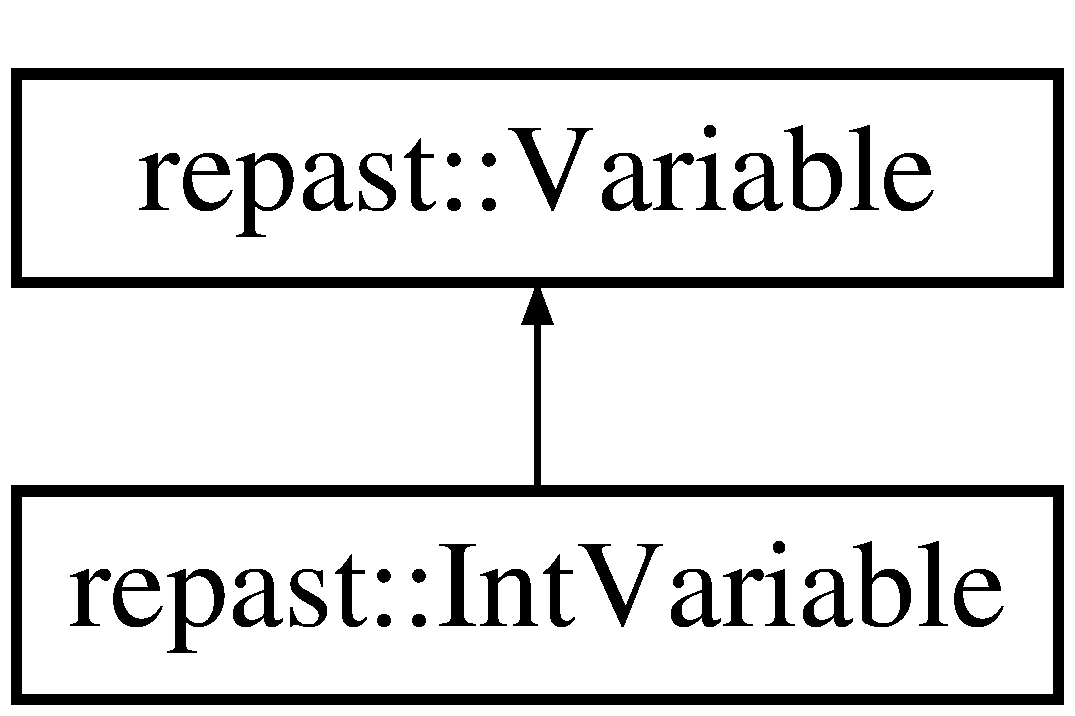
\includegraphics[height=2.000000cm]{classrepast_1_1_int_variable}
\end{center}
\end{figure}
\subsection*{Public Member Functions}
\begin{DoxyCompactItemize}
\item 
virtual void \hyperlink{classrepast_1_1_int_variable_a21701e82f63a4ae02ea5edf24c2d39f6}{write} (size\-\_\-t index, std\-::ofstream \&out)
\begin{DoxyCompactList}\small\item\em Writes the data at the specified index to the specified ofstream. \end{DoxyCompactList}\item 
virtual void \hyperlink{classrepast_1_1_int_variable_a20ff24e57f87be9ea44b312630f13d1f}{insert} (double $\ast$array, size\-\_\-t size)
\begin{DoxyCompactList}\small\item\em Inserts all the doubles in the double array into the collection of data stored in this \hyperlink{classrepast_1_1_variable}{Variable}. \end{DoxyCompactList}\item 
virtual void \hyperlink{classrepast_1_1_int_variable_a22de6afa3d3e50b4f322b9667e7eb3a2}{insert} (int $\ast$array, size\-\_\-t size)
\begin{DoxyCompactList}\small\item\em Inserts all the ints in the int array into the collection of data stored in this \hyperlink{classrepast_1_1_variable}{Variable}. \end{DoxyCompactList}\item 
\hypertarget{classrepast_1_1_int_variable_a1b22f400a25e7afeb347d3f542000cca}{virtual void \hyperlink{classrepast_1_1_int_variable_a1b22f400a25e7afeb347d3f542000cca}{clear} ()}\label{classrepast_1_1_int_variable_a1b22f400a25e7afeb347d3f542000cca}

\begin{DoxyCompactList}\small\item\em Clears this \hyperlink{classrepast_1_1_variable}{Variable} of all the data stored in it. \end{DoxyCompactList}\end{DoxyCompactItemize}


\subsection{Detailed Description}
Used in \hyperlink{classrepast_1_1_s_v_data_set}{S\-V\-Data\-Set} to manage integer data. 

\subsection{Member Function Documentation}
\hypertarget{classrepast_1_1_int_variable_a20ff24e57f87be9ea44b312630f13d1f}{\index{repast\-::\-Int\-Variable@{repast\-::\-Int\-Variable}!insert@{insert}}
\index{insert@{insert}!repast::IntVariable@{repast\-::\-Int\-Variable}}
\subsubsection[{insert}]{\setlength{\rightskip}{0pt plus 5cm}void repast\-::\-Int\-Variable\-::insert (
\begin{DoxyParamCaption}
\item[{double $\ast$}]{array, }
\item[{size\-\_\-t}]{size}
\end{DoxyParamCaption}
)\hspace{0.3cm}{\ttfamily [virtual]}}}\label{classrepast_1_1_int_variable_a20ff24e57f87be9ea44b312630f13d1f}


Inserts all the doubles in the double array into the collection of data stored in this \hyperlink{classrepast_1_1_variable}{Variable}. 


\begin{DoxyParams}{Parameters}
{\em array} & the array to insert \\
\hline
{\em size} & the size of the array \\
\hline
\end{DoxyParams}


Implements \hyperlink{classrepast_1_1_variable_ac87aada07f0b7ee34d6fbd2486016eb8}{repast\-::\-Variable}.

\hypertarget{classrepast_1_1_int_variable_a22de6afa3d3e50b4f322b9667e7eb3a2}{\index{repast\-::\-Int\-Variable@{repast\-::\-Int\-Variable}!insert@{insert}}
\index{insert@{insert}!repast::IntVariable@{repast\-::\-Int\-Variable}}
\subsubsection[{insert}]{\setlength{\rightskip}{0pt plus 5cm}void repast\-::\-Int\-Variable\-::insert (
\begin{DoxyParamCaption}
\item[{int $\ast$}]{array, }
\item[{size\-\_\-t}]{size}
\end{DoxyParamCaption}
)\hspace{0.3cm}{\ttfamily [virtual]}}}\label{classrepast_1_1_int_variable_a22de6afa3d3e50b4f322b9667e7eb3a2}


Inserts all the ints in the int array into the collection of data stored in this \hyperlink{classrepast_1_1_variable}{Variable}. 


\begin{DoxyParams}{Parameters}
{\em array} & the array to insert \\
\hline
{\em size} & the size of the array \\
\hline
\end{DoxyParams}


Implements \hyperlink{classrepast_1_1_variable_a5f625f2652dcbc9c1910539923475936}{repast\-::\-Variable}.

\hypertarget{classrepast_1_1_int_variable_a21701e82f63a4ae02ea5edf24c2d39f6}{\index{repast\-::\-Int\-Variable@{repast\-::\-Int\-Variable}!write@{write}}
\index{write@{write}!repast::IntVariable@{repast\-::\-Int\-Variable}}
\subsubsection[{write}]{\setlength{\rightskip}{0pt plus 5cm}void repast\-::\-Int\-Variable\-::write (
\begin{DoxyParamCaption}
\item[{size\-\_\-t}]{index, }
\item[{std\-::ofstream \&}]{out}
\end{DoxyParamCaption}
)\hspace{0.3cm}{\ttfamily [virtual]}}}\label{classrepast_1_1_int_variable_a21701e82f63a4ae02ea5edf24c2d39f6}


Writes the data at the specified index to the specified ofstream. 


\begin{DoxyParams}{Parameters}
{\em index} & the index of the data to write \\
\hline
{\em out} & the ofstream to write the data to \\
\hline
\end{DoxyParams}


Implements \hyperlink{classrepast_1_1_variable_aa72da48bdca530dd7878b912254568e0}{repast\-::\-Variable}.



The documentation for this class was generated from the following files\-:\begin{DoxyCompactItemize}
\item 
repast\-\_\-hpc/Variable.\-h\item 
repast\-\_\-hpc/Variable.\-cpp\end{DoxyCompactItemize}

\hypertarget{structrepast_1_1_is_agent_type}{\section{repast\-:\-:Is\-Agent\-Type$<$ T $>$ Struct Template Reference}
\label{structrepast_1_1_is_agent_type}\index{repast\-::\-Is\-Agent\-Type$<$ T $>$@{repast\-::\-Is\-Agent\-Type$<$ T $>$}}
}


Struct that allows filtering by \hyperlink{classrepast_1_1_agent}{Agent} Type.  




{\ttfamily \#include $<$Agent\-Id.\-h$>$}

\subsection*{Public Member Functions}
\begin{DoxyCompactItemize}
\item 
\hypertarget{structrepast_1_1_is_agent_type_a9da2d4d5b5ec3be54e01ac6849f1cb42}{{\bfseries Is\-Agent\-Type} (int type\-Id)}\label{structrepast_1_1_is_agent_type_a9da2d4d5b5ec3be54e01ac6849f1cb42}

\item 
\hypertarget{structrepast_1_1_is_agent_type_a66d0e0e92abd3a129c739dac0b1f40eb}{bool {\bfseries operator()} (const boost\-::shared\-\_\-ptr$<$ T $>$ \&ptr)}\label{structrepast_1_1_is_agent_type_a66d0e0e92abd3a129c739dac0b1f40eb}

\item 
\hypertarget{structrepast_1_1_is_agent_type_a2eccc7a054094a2702307032462b1907}{bool {\bfseries operator()} (const T $\ast$agent)}\label{structrepast_1_1_is_agent_type_a2eccc7a054094a2702307032462b1907}

\end{DoxyCompactItemize}
\subsection*{Public Attributes}
\begin{DoxyCompactItemize}
\item 
\hypertarget{structrepast_1_1_is_agent_type_ad72641323f727069fe4a1b5a07d15ec4}{int {\bfseries \-\_\-type\-Id}}\label{structrepast_1_1_is_agent_type_ad72641323f727069fe4a1b5a07d15ec4}

\end{DoxyCompactItemize}


\subsection{Detailed Description}
\subsubsection*{template$<$typename T$>$struct repast\-::\-Is\-Agent\-Type$<$ T $>$}

Struct that allows filtering by \hyperlink{classrepast_1_1_agent}{Agent} Type. 

The documentation for this struct was generated from the following file\-:\begin{DoxyCompactItemize}
\item 
repast\-\_\-hpc/Agent\-Id.\-h\end{DoxyCompactItemize}

\hypertarget{structrepast_1_1_is_local_agent}{\section{repast\-:\-:Is\-Local\-Agent$<$ T $>$ Struct Template Reference}
\label{structrepast_1_1_is_local_agent}\index{repast\-::\-Is\-Local\-Agent$<$ T $>$@{repast\-::\-Is\-Local\-Agent$<$ T $>$}}
}


Used in a filter iterator to filter on local agents only.  




{\ttfamily \#include $<$Shared\-Context.\-h$>$}

\subsection*{Public Member Functions}
\begin{DoxyCompactItemize}
\item 
\hypertarget{structrepast_1_1_is_local_agent_ad29d7ef8ffc1d238fd9468277b7c5f03}{{\bfseries Is\-Local\-Agent} (int rank\-In\-Communicator)}\label{structrepast_1_1_is_local_agent_ad29d7ef8ffc1d238fd9468277b7c5f03}

\item 
\hypertarget{structrepast_1_1_is_local_agent_a55212e849b4a59eebcf2a0bd1c9b3a96}{bool {\bfseries operator()} (const boost\-::shared\-\_\-ptr$<$ T $>$ \&ptr)}\label{structrepast_1_1_is_local_agent_a55212e849b4a59eebcf2a0bd1c9b3a96}

\end{DoxyCompactItemize}
\subsection*{Public Attributes}
\begin{DoxyCompactItemize}
\item 
\hypertarget{structrepast_1_1_is_local_agent_a2cb93804105c47d43f8085f4e699687a}{int {\bfseries rank}}\label{structrepast_1_1_is_local_agent_a2cb93804105c47d43f8085f4e699687a}

\end{DoxyCompactItemize}


\subsection{Detailed Description}
\subsubsection*{template$<$typename T$>$struct repast\-::\-Is\-Local\-Agent$<$ T $>$}

Used in a filter iterator to filter on local agents only. 

The documentation for this struct was generated from the following file\-:\begin{DoxyCompactItemize}
\item 
repast\-\_\-hpc/Shared\-Context.\-h\end{DoxyCompactItemize}

\hypertarget{structrepast_1_1_is_not_type}{\section{repast\-:\-:Is\-Not\-Type$<$ T $>$ Struct Template Reference}
\label{structrepast_1_1_is_not_type}\index{repast\-::\-Is\-Not\-Type$<$ T $>$@{repast\-::\-Is\-Not\-Type$<$ T $>$}}
}


Struct that allows filtering by !(\hyperlink{classrepast_1_1_agent}{Agent} Type)  




{\ttfamily \#include $<$Agent\-Id.\-h$>$}

\subsection*{Public Member Functions}
\begin{DoxyCompactItemize}
\item 
\hypertarget{structrepast_1_1_is_not_type_a234ea8aeff3917ef9a3d94b3c14eb369}{{\bfseries Is\-Not\-Type} (int type\-Id)}\label{structrepast_1_1_is_not_type_a234ea8aeff3917ef9a3d94b3c14eb369}

\item 
\hypertarget{structrepast_1_1_is_not_type_a0b2ee838f9eca383b54e2a581fe47f94}{bool {\bfseries operator()} (const boost\-::shared\-\_\-ptr$<$ T $>$ \&ptr)}\label{structrepast_1_1_is_not_type_a0b2ee838f9eca383b54e2a581fe47f94}

\item 
\hypertarget{structrepast_1_1_is_not_type_a24299271f22793fd7d4a76f94fb88e70}{bool {\bfseries operator()} (const T $\ast$agent)}\label{structrepast_1_1_is_not_type_a24299271f22793fd7d4a76f94fb88e70}

\end{DoxyCompactItemize}
\subsection*{Public Attributes}
\begin{DoxyCompactItemize}
\item 
\hypertarget{structrepast_1_1_is_not_type_a58ce9b0f12b75b1fead7bff825f8d97e}{int {\bfseries \-\_\-type\-Id}}\label{structrepast_1_1_is_not_type_a58ce9b0f12b75b1fead7bff825f8d97e}

\end{DoxyCompactItemize}


\subsection{Detailed Description}
\subsubsection*{template$<$typename T$>$struct repast\-::\-Is\-Not\-Type$<$ T $>$}

Struct that allows filtering by !(\hyperlink{classrepast_1_1_agent}{Agent} Type) 

The documentation for this struct was generated from the following file\-:\begin{DoxyCompactItemize}
\item 
repast\-\_\-hpc/Agent\-Id.\-h\end{DoxyCompactItemize}

\hypertarget{classrepast_1_1_item_receipt}{\section{repast\-:\-:Item\-Receipt$<$ E $>$ Class Template Reference}
\label{classrepast_1_1_item_receipt}\index{repast\-::\-Item\-Receipt$<$ E $>$@{repast\-::\-Item\-Receipt$<$ E $>$}}
}


{\itshape D\-E\-P\-R\-E\-C\-A\-T\-E\-D} Receipt for edges Class used to receive edges being sent.  




{\ttfamily \#include $<$Shared\-Network.\-h$>$}

\subsection*{Public Member Functions}
\begin{DoxyCompactItemize}
\item 
\hypertarget{classrepast_1_1_item_receipt_a88b27d495278d41c0a427840e1571a83}{{\bfseries Item\-Receipt} (int source)}\label{classrepast_1_1_item_receipt_a88b27d495278d41c0a427840e1571a83}

\end{DoxyCompactItemize}
\subsection*{Public Attributes}
\begin{DoxyCompactItemize}
\item 
\hypertarget{classrepast_1_1_item_receipt_aa72eac73d1a8eee74efc7e100e503330}{std\-::vector$<$ E $>$ {\bfseries items}}\label{classrepast_1_1_item_receipt_aa72eac73d1a8eee74efc7e100e503330}

\item 
\hypertarget{classrepast_1_1_item_receipt_ae7a0c999195107c1dc66dfd9cf862958}{int {\bfseries source\-\_\-}}\label{classrepast_1_1_item_receipt_ae7a0c999195107c1dc66dfd9cf862958}

\end{DoxyCompactItemize}


\subsection{Detailed Description}
\subsubsection*{template$<$typename E$>$class repast\-::\-Item\-Receipt$<$ E $>$}

{\itshape D\-E\-P\-R\-E\-C\-A\-T\-E\-D} Receipt for edges Class used to receive edges being sent. 

\begin{DoxyRefDesc}{Deprecated}
\item[\hyperlink{deprecated__deprecated000004}{Deprecated}]As of Version 2.\-0 replaced by \hyperlink{classrepast_1_1_projection_info_packet}{Projection\-Info\-Packet} objects. \end{DoxyRefDesc}


The documentation for this class was generated from the following file\-:\begin{DoxyCompactItemize}
\item 
repast\-\_\-hpc/Shared\-Network.\-h\end{DoxyCompactItemize}

\hypertarget{classrepast_1_1_k_e_builder}{\section{repast\-:\-:K\-E\-Builder$<$ V, E, Ec, Ec\-M $>$ Class Template Reference}
\label{classrepast_1_1_k_e_builder}\index{repast\-::\-K\-E\-Builder$<$ V, E, Ec, Ec\-M $>$@{repast\-::\-K\-E\-Builder$<$ V, E, Ec, Ec\-M $>$}}
}


Buils K\-E type networks.  




{\ttfamily \#include $<$Network\-Builder.\-h$>$}

\subsection*{Public Member Functions}
\begin{DoxyCompactItemize}
\item 
void \hyperlink{classrepast_1_1_k_e_builder_a89b6f648c29bb59fd0b3f2495b9c2fc0}{build} (\hyperlink{classrepast_1_1_properties}{repast\-::\-Properties} \&props, \hyperlink{classrepast_1_1_graph}{repast\-::\-Graph}$<$ V, E, Ec, Ec\-M $>$ $\ast$graph)
\begin{DoxyCompactList}\small\item\em Builds the network. \end{DoxyCompactList}\end{DoxyCompactItemize}


\subsection{Detailed Description}
\subsubsection*{template$<$typename V, typename E, typename Ec, typename Ec\-M$>$class repast\-::\-K\-E\-Builder$<$ V, E, Ec, Ec\-M $>$}

Buils K\-E type networks. 

See Klemm and Eguiluz, \char`\"{}\-Growing scale-\/free network with small world behavior\char`\"{} in Phys. Rev. E 65. 

\subsection{Member Function Documentation}
\hypertarget{classrepast_1_1_k_e_builder_a89b6f648c29bb59fd0b3f2495b9c2fc0}{\index{repast\-::\-K\-E\-Builder@{repast\-::\-K\-E\-Builder}!build@{build}}
\index{build@{build}!repast::KEBuilder@{repast\-::\-K\-E\-Builder}}
\subsubsection[{build}]{\setlength{\rightskip}{0pt plus 5cm}template$<$typename V , typename E , typename Ec , typename Ec\-M $>$ void {\bf repast\-::\-K\-E\-Builder}$<$ V, E, Ec, Ec\-M $>$\-::build (
\begin{DoxyParamCaption}
\item[{{\bf repast\-::\-Properties} \&}]{props, }
\item[{{\bf repast\-::\-Graph}$<$ V, E, Ec, Ec\-M $>$ $\ast$}]{graph}
\end{DoxyParamCaption}
)}}\label{classrepast_1_1_k_e_builder_a89b6f648c29bb59fd0b3f2495b9c2fc0}


Builds the network. 

The graph should contains the vertices the build the network with and props should contain the M values.


\begin{DoxyParams}{Parameters}
{\em props} & a \hyperlink{classrepast_1_1_properties}{Properties} containing a property \char`\"{}ke.\-model.\-m\char`\"{} that specifies the M value. \\
\hline
{\em graph} & the graph to build the network \\
\hline
\end{DoxyParams}


The documentation for this class was generated from the following file\-:\begin{DoxyCompactItemize}
\item 
repast\-\_\-hpc/Network\-Builder.\-h\end{DoxyCompactItemize}

\hypertarget{structrepast_1_1_key_getter}{\section{repast\-:\-:Key\-Getter Struct Reference}
\label{structrepast_1_1_key_getter}\index{repast\-::\-Key\-Getter@{repast\-::\-Key\-Getter}}
}


Unary function used in a transform\-\_\-iterator that allows the map iterator to return the keys.  




{\ttfamily \#include $<$Properties.\-h$>$}

Inheritance diagram for repast\-:\-:Key\-Getter\-:\begin{figure}[H]
\begin{center}
\leavevmode
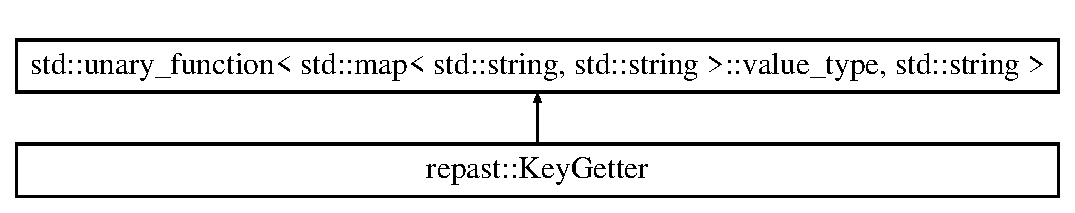
\includegraphics[height=2.000000cm]{structrepast_1_1_key_getter}
\end{center}
\end{figure}
\subsection*{Public Member Functions}
\begin{DoxyCompactItemize}
\item 
\hypertarget{structrepast_1_1_key_getter_a8e4c794acce2375ef4e3015443b9a496}{std\-::string {\bfseries operator()} (const std\-::map$<$ std\-::string, std\-::string $>$\-::value\-\_\-type \&value) const }\label{structrepast_1_1_key_getter_a8e4c794acce2375ef4e3015443b9a496}

\end{DoxyCompactItemize}


\subsection{Detailed Description}
Unary function used in a transform\-\_\-iterator that allows the map iterator to return the keys. 

The documentation for this struct was generated from the following files\-:\begin{DoxyCompactItemize}
\item 
repast\-\_\-hpc/Properties.\-h\item 
repast\-\_\-hpc/Properties.\-cpp\end{DoxyCompactItemize}

\hypertarget{class_log4_c_l}{\section{Log4\-C\-L Class Reference}
\label{class_log4_c_l}\index{Log4\-C\-L@{Log4\-C\-L}}
}
\subsection*{Public Member Functions}
\begin{DoxyCompactItemize}
\item 
\hypertarget{class_log4_c_l_acf274891399834114393e5440e54d78e}{\hyperlink{class_logger}{Logger} \& {\bfseries get\-\_\-logger} (std\-::string logger\-\_\-name)}\label{class_log4_c_l_acf274891399834114393e5440e54d78e}

\item 
\hypertarget{class_log4_c_l_a79dd02857dbcee7b00431e8508390910}{void {\bfseries close} ()}\label{class_log4_c_l_a79dd02857dbcee7b00431e8508390910}

\end{DoxyCompactItemize}
\subsection*{Static Public Member Functions}
\begin{DoxyCompactItemize}
\item 
\hypertarget{class_log4_c_l_a3657ff59071abde1631607884a04f366}{static \hyperlink{class_log4_c_l}{Log4\-C\-L} $\ast$ {\bfseries instance} ()}\label{class_log4_c_l_a3657ff59071abde1631607884a04f366}

\item 
\hypertarget{class_log4_c_l_aba1953ed8d7bc7c38ccea87c510b952c}{static void {\bfseries configure} (int, const std\-::string \&, boost\-::mpi\-::communicator $\ast$comm=0, int max\-Config\-File\-Size=M\-A\-X\-\_\-\-C\-O\-N\-F\-I\-G\-\_\-\-F\-I\-L\-E\-\_\-\-S\-I\-Z\-E)}\label{class_log4_c_l_aba1953ed8d7bc7c38ccea87c510b952c}

\item 
\hypertarget{class_log4_c_l_a3ccf6dcd6d42d3ad49e60cbbce2b57a3}{static void {\bfseries configure} (int)}\label{class_log4_c_l_a3ccf6dcd6d42d3ad49e60cbbce2b57a3}

\end{DoxyCompactItemize}
\subsection*{Protected Member Functions}
\begin{DoxyCompactItemize}
\item 
\hypertarget{class_log4_c_l_ab502e31e01c50cc11dc30cb400471561}{{\bfseries Log4\-C\-L} (int)}\label{class_log4_c_l_ab502e31e01c50cc11dc30cb400471561}

\end{DoxyCompactItemize}
\subsection*{Friends}
\begin{DoxyCompactItemize}
\item 
\hypertarget{class_log4_c_l_af0e54cc350bb8e25a6a22bf3f38f21c5}{class {\bfseries Log4\-C\-L\-Configurator}}\label{class_log4_c_l_af0e54cc350bb8e25a6a22bf3f38f21c5}

\end{DoxyCompactItemize}


The documentation for this class was generated from the following files\-:\begin{DoxyCompactItemize}
\item 
repast\-\_\-hpc/logger.\-h\item 
repast\-\_\-hpc/logger.\-cpp\end{DoxyCompactItemize}

\hypertarget{class_log4_c_l_configurator}{\section{Log4\-C\-L\-Configurator Class Reference}
\label{class_log4_c_l_configurator}\index{Log4\-C\-L\-Configurator@{Log4\-C\-L\-Configurator}}
}
\subsection*{Public Member Functions}
\begin{DoxyCompactItemize}
\item 
\hypertarget{class_log4_c_l_configurator_a3a3027bf647a1ee2e3103a36cf59cbf5}{\hyperlink{class_log4_c_l}{Log4\-C\-L} $\ast$ {\bfseries configure} (const std\-::string \&config\-\_\-file, int proc\-\_\-id, boost\-::mpi\-::communicator $\ast$comm=0, int max\-Config\-File\-Size=M\-A\-X\-\_\-\-C\-O\-N\-F\-I\-G\-\_\-\-F\-I\-L\-E\-\_\-\-S\-I\-Z\-E)}\label{class_log4_c_l_configurator_a3a3027bf647a1ee2e3103a36cf59cbf5}

\end{DoxyCompactItemize}


The documentation for this class was generated from the following files\-:\begin{DoxyCompactItemize}
\item 
repast\-\_\-hpc/logger.\-h\item 
repast\-\_\-hpc/logger.\-cpp\end{DoxyCompactItemize}

\hypertarget{class_logger}{\section{Logger Class Reference}
\label{class_logger}\index{Logger@{Logger}}
}
\subsection*{Public Member Functions}
\begin{DoxyCompactItemize}
\item 
\hypertarget{class_logger_ad4bef2613eb1eba924d90561c646203a}{{\bfseries Logger} (const std\-::string, L\-O\-G\-\_\-\-L\-E\-V\-E\-L, int proc\-\_\-id)}\label{class_logger_ad4bef2613eb1eba924d90561c646203a}

\item 
\hypertarget{class_logger_ac05e48b3ad9831593c664a7e1a198e47}{void {\bfseries log} (L\-O\-G\-\_\-\-L\-E\-V\-E\-L, const std\-::string msg)}\label{class_logger_ac05e48b3ad9831593c664a7e1a198e47}

\item 
\hypertarget{class_logger_afee2bab560c2db0190c980884d33868c}{void {\bfseries close} ()}\label{class_logger_afee2bab560c2db0190c980884d33868c}

\item 
\hypertarget{class_logger_a7075e9cf5373d978dd346040f09043a8}{void {\bfseries add\-\_\-appender} (\hyperlink{class_appender}{Appender} $\ast$appender)}\label{class_logger_a7075e9cf5373d978dd346040f09043a8}

\end{DoxyCompactItemize}


The documentation for this class was generated from the following files\-:\begin{DoxyCompactItemize}
\item 
repast\-\_\-hpc/logger.\-h\item 
repast\-\_\-hpc/logger.\-cpp\end{DoxyCompactItemize}

\hypertarget{classrepast_1_1_matrix}{\section{repast\-:\-:Matrix$<$ T $>$ Class Template Reference}
\label{classrepast_1_1_matrix}\index{repast\-::\-Matrix$<$ T $>$@{repast\-::\-Matrix$<$ T $>$}}
}


Base class for matrix implementations.  




{\ttfamily \#include $<$matrix.\-h$>$}

Inheritance diagram for repast\-:\-:Matrix$<$ T $>$\-:\begin{figure}[H]
\begin{center}
\leavevmode
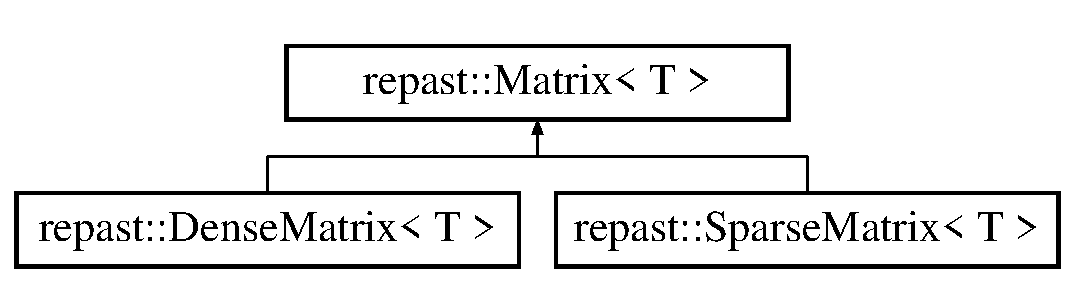
\includegraphics[height=2.000000cm]{classrepast_1_1_matrix}
\end{center}
\end{figure}
\subsection*{Public Member Functions}
\begin{DoxyCompactItemize}
\item 
\hyperlink{classrepast_1_1_matrix_a65c52c43c430b1a78c56c006b4559ce3}{Matrix} (const \hyperlink{classrepast_1_1_point}{Point}$<$ int $>$ \&size, const T \&\hyperlink{classrepast_1_1_matrix_ab7d7c37233ead4a6a68feaf344b3ff38}{default\-Value}=T())
\begin{DoxyCompactList}\small\item\em Creates a matrix of the specified size and with the specified default value. \end{DoxyCompactList}\item 
\hypertarget{classrepast_1_1_matrix_a865d67868c32af9e4944c84431ec29a2}{virtual T \& \hyperlink{classrepast_1_1_matrix_a865d67868c32af9e4944c84431ec29a2}{get} (const \hyperlink{classrepast_1_1_point}{Point}$<$ int $>$ \&index)=0}\label{classrepast_1_1_matrix_a865d67868c32af9e4944c84431ec29a2}

\begin{DoxyCompactList}\small\item\em Gets the value at the specified index. \end{DoxyCompactList}\item 
\hypertarget{classrepast_1_1_matrix_a5c7735a078a35f0b9deca407e546ab55}{virtual void \hyperlink{classrepast_1_1_matrix_a5c7735a078a35f0b9deca407e546ab55}{set} (const T \&value, const \hyperlink{classrepast_1_1_point}{Point}$<$ int $>$ \&index)=0}\label{classrepast_1_1_matrix_a5c7735a078a35f0b9deca407e546ab55}

\begin{DoxyCompactList}\small\item\em Sets the value at the specified index. \end{DoxyCompactList}\item 
\hypertarget{classrepast_1_1_matrix_a9cb528d30b1d646d6ca742c3b76a9285}{T \& {\bfseries operator\mbox{[}$\,$\mbox{]}} (const \hyperlink{classrepast_1_1_point}{Point}$<$ int $>$ \&index)}\label{classrepast_1_1_matrix_a9cb528d30b1d646d6ca742c3b76a9285}

\item 
\hypertarget{classrepast_1_1_matrix_a63932af327a9cb1e0501dc183fc034b3}{const T \& {\bfseries operator\mbox{[}$\,$\mbox{]}} (const \hyperlink{classrepast_1_1_point}{Point}$<$ int $>$ \&index) const }\label{classrepast_1_1_matrix_a63932af327a9cb1e0501dc183fc034b3}

\item 
\hypertarget{classrepast_1_1_matrix_ab7d7c37233ead4a6a68feaf344b3ff38}{const T \& \hyperlink{classrepast_1_1_matrix_ab7d7c37233ead4a6a68feaf344b3ff38}{default\-Value} () const }\label{classrepast_1_1_matrix_ab7d7c37233ead4a6a68feaf344b3ff38}

\begin{DoxyCompactList}\small\item\em Gets the default value of any unset matrix cell. \end{DoxyCompactList}\item 
const \hyperlink{classrepast_1_1_point}{Point}$<$ int $>$ \hyperlink{classrepast_1_1_matrix_aa81d61acab94e9de748a647ed3ef535f}{shape} () const 
\begin{DoxyCompactList}\small\item\em Gets the shape (i.\-e. \end{DoxyCompactList}\end{DoxyCompactItemize}
\subsection*{Protected Member Functions}
\begin{DoxyCompactItemize}
\item 
\hypertarget{classrepast_1_1_matrix_af7dd562d3d48904888c131ce3b53e4fd}{int {\bfseries calc\-Index} (const \hyperlink{classrepast_1_1_point}{Point}$<$ int $>$ \&index)}\label{classrepast_1_1_matrix_af7dd562d3d48904888c131ce3b53e4fd}

\item 
\hypertarget{classrepast_1_1_matrix_ae5b989256328e66805b51bb7b27edc53}{void {\bfseries bounds\-Check} (const \hyperlink{classrepast_1_1_point}{Point}$<$ int $>$ \&index)}\label{classrepast_1_1_matrix_ae5b989256328e66805b51bb7b27edc53}

\item 
\hypertarget{classrepast_1_1_matrix_a21922251aaa359c5a853640f60e4a0fc}{void {\bfseries create} ()}\label{classrepast_1_1_matrix_a21922251aaa359c5a853640f60e4a0fc}

\end{DoxyCompactItemize}
\subsection*{Protected Attributes}
\begin{DoxyCompactItemize}
\item 
\hypertarget{classrepast_1_1_matrix_ad63eee84ab11e3d46e45efad8d7e842f}{int $\ast$ {\bfseries stride}}\label{classrepast_1_1_matrix_ad63eee84ab11e3d46e45efad8d7e842f}

\item 
\hypertarget{classrepast_1_1_matrix_a7163c6a75fdb8615a5cc1f6f0d801317}{T {\bfseries def\-Value}}\label{classrepast_1_1_matrix_a7163c6a75fdb8615a5cc1f6f0d801317}

\item 
\hypertarget{classrepast_1_1_matrix_a7e14526c496b2c3b6969efe762064010}{\hyperlink{classrepast_1_1_point}{Point}$<$ int $>$ {\bfseries \-\_\-size}}\label{classrepast_1_1_matrix_a7e14526c496b2c3b6969efe762064010}

\item 
\hypertarget{classrepast_1_1_matrix_aebf77b607e15cefe4189d3c3e6f50ef0}{int {\bfseries d\-Count}}\label{classrepast_1_1_matrix_aebf77b607e15cefe4189d3c3e6f50ef0}

\end{DoxyCompactItemize}


\subsection{Detailed Description}
\subsubsection*{template$<$typename T$>$class repast\-::\-Matrix$<$ T $>$}

Base class for matrix implementations. 

\subsection{Constructor \& Destructor Documentation}
\hypertarget{classrepast_1_1_matrix_a65c52c43c430b1a78c56c006b4559ce3}{\index{repast\-::\-Matrix@{repast\-::\-Matrix}!Matrix@{Matrix}}
\index{Matrix@{Matrix}!repast::Matrix@{repast\-::\-Matrix}}
\subsubsection[{Matrix}]{\setlength{\rightskip}{0pt plus 5cm}template$<$typename T$>$ {\bf repast\-::\-Matrix}$<$ T $>$\-::{\bf Matrix} (
\begin{DoxyParamCaption}
\item[{const {\bf Point}$<$ int $>$ \&}]{size, }
\item[{const T \&}]{default\-Value = {\ttfamily T()}}
\end{DoxyParamCaption}
)\hspace{0.3cm}{\ttfamily [explicit]}}}\label{classrepast_1_1_matrix_a65c52c43c430b1a78c56c006b4559ce3}


Creates a matrix of the specified size and with the specified default value. 


\begin{DoxyParams}{Parameters}
{\em size} & the size of the matrix in each dimension \\
\hline
\end{DoxyParams}


\subsection{Member Function Documentation}
\hypertarget{classrepast_1_1_matrix_aa81d61acab94e9de748a647ed3ef535f}{\index{repast\-::\-Matrix@{repast\-::\-Matrix}!shape@{shape}}
\index{shape@{shape}!repast::Matrix@{repast\-::\-Matrix}}
\subsubsection[{shape}]{\setlength{\rightskip}{0pt plus 5cm}template$<$typename T$>$ const {\bf Point}$<$int$>$ {\bf repast\-::\-Matrix}$<$ T $>$\-::shape (
\begin{DoxyParamCaption}
{}
\end{DoxyParamCaption}
) const\hspace{0.3cm}{\ttfamily [inline]}}}\label{classrepast_1_1_matrix_aa81d61acab94e9de748a647ed3ef535f}


Gets the shape (i.\-e. 

the length of each dimensions) of the matrix. 

The documentation for this class was generated from the following file\-:\begin{DoxyCompactItemize}
\item 
repast\-\_\-hpc/matrix.\-h\end{DoxyCompactItemize}

\hypertarget{classrepast_1_1_method_functor}{\section{repast\-:\-:Method\-Functor$<$ T $>$ Class Template Reference}
\label{classrepast_1_1_method_functor}\index{repast\-::\-Method\-Functor$<$ T $>$@{repast\-::\-Method\-Functor$<$ T $>$}}
}


Adapts a no-\/arg method call on an object instance to a \hyperlink{classrepast_1_1_functor}{Functor} interface.  




{\ttfamily \#include $<$Schedule.\-h$>$}

Inheritance diagram for repast\-:\-:Method\-Functor$<$ T $>$\-:\begin{figure}[H]
\begin{center}
\leavevmode
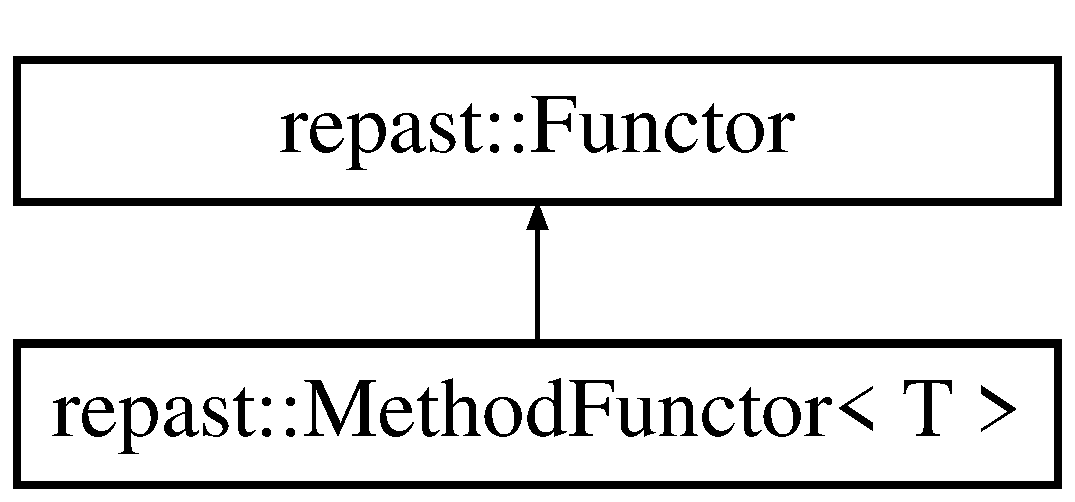
\includegraphics[height=2.000000cm]{classrepast_1_1_method_functor}
\end{center}
\end{figure}
\subsection*{Public Member Functions}
\begin{DoxyCompactItemize}
\item 
\hypertarget{classrepast_1_1_method_functor_aea76fb8700d36f0978cd3b5efa995bb3}{{\bfseries Method\-Functor} (T $\ast$\-\_\-obj, void(T\-::$\ast$\-\_\-fptr)())}\label{classrepast_1_1_method_functor_aea76fb8700d36f0978cd3b5efa995bb3}

\item 
\hypertarget{classrepast_1_1_method_functor_ab335eb6d9a05e2a470dab88d5e573823}{void {\bfseries operator()} ()}\label{classrepast_1_1_method_functor_ab335eb6d9a05e2a470dab88d5e573823}

\end{DoxyCompactItemize}


\subsection{Detailed Description}
\subsubsection*{template$<$typename T$>$class repast\-::\-Method\-Functor$<$ T $>$}

Adapts a no-\/arg method call on an object instance to a \hyperlink{classrepast_1_1_functor}{Functor} interface. 

This is used by the \hyperlink{classrepast_1_1_schedule}{Schedule} code to schedule method calls on objects.


\begin{DoxyTemplParams}{Template Parameters}
{\em T} & the object type on which the call will be made. \\
\hline
\end{DoxyTemplParams}


The documentation for this class was generated from the following file\-:\begin{DoxyCompactItemize}
\item 
repast\-\_\-hpc/Schedule.\-h\end{DoxyCompactItemize}

\hypertarget{classrepast_1_1_moore2_d_grid_query}{\section{repast\-:\-:Moore2\-D\-Grid\-Query$<$ T $>$ Class Template Reference}
\label{classrepast_1_1_moore2_d_grid_query}\index{repast\-::\-Moore2\-D\-Grid\-Query$<$ T $>$@{repast\-::\-Moore2\-D\-Grid\-Query$<$ T $>$}}
}


Neighborhood query that gathers neighbors in a Moore (N, S, E, W, N\-E, etc.) neighborhood.  




{\ttfamily \#include $<$Moore2\-D\-Grid\-Query.\-h$>$}

Inheritance diagram for repast\-:\-:Moore2\-D\-Grid\-Query$<$ T $>$\-:\begin{figure}[H]
\begin{center}
\leavevmode
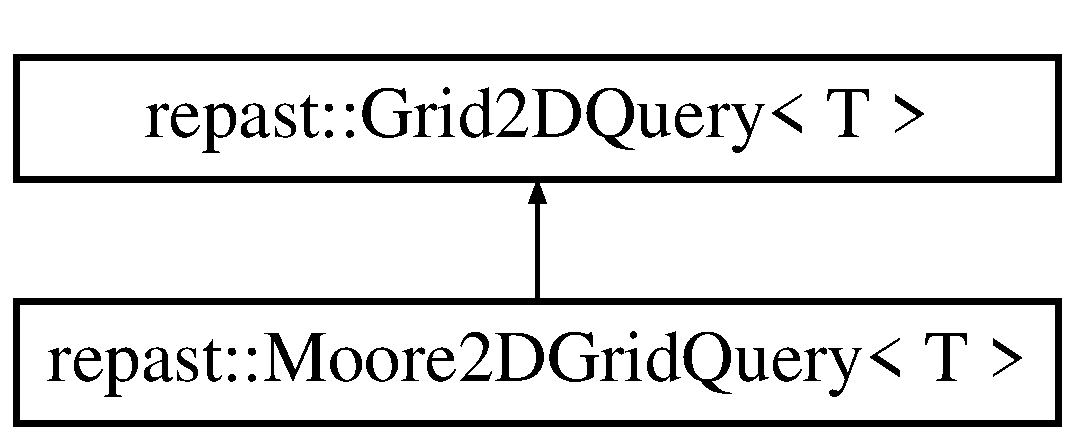
\includegraphics[height=2.000000cm]{classrepast_1_1_moore2_d_grid_query}
\end{center}
\end{figure}
\subsection*{Public Member Functions}
\begin{DoxyCompactItemize}
\item 
\hypertarget{classrepast_1_1_moore2_d_grid_query_a427a50dbe9631d9c4f7353bdf5b94bd3}{\hyperlink{classrepast_1_1_moore2_d_grid_query_a427a50dbe9631d9c4f7353bdf5b94bd3}{Moore2\-D\-Grid\-Query} (const \hyperlink{classrepast_1_1_grid}{Grid}$<$ T, int $>$ $\ast$grid)}\label{classrepast_1_1_moore2_d_grid_query_a427a50dbe9631d9c4f7353bdf5b94bd3}

\begin{DoxyCompactList}\small\item\em Creates \hyperlink{classrepast_1_1_moore2_d_grid_query}{Moore2\-D\-Grid\-Query} that will query the specified \hyperlink{classrepast_1_1_grid}{Grid}. \end{DoxyCompactList}\item 
virtual void \hyperlink{classrepast_1_1_moore2_d_grid_query_a43cd6c0a6cd2c3f1932bbaa5595b0576}{query} (const \hyperlink{classrepast_1_1_point}{Point}$<$ int $>$ \&center, int range, bool include\-Center, std\-::vector$<$ T $\ast$ $>$ \&out) const 
\begin{DoxyCompactList}\small\item\em Queries the \hyperlink{classrepast_1_1_grid}{Grid} for the Moore neighbors surrounding the center point within a specified range. \end{DoxyCompactList}\end{DoxyCompactItemize}
\subsection*{Additional Inherited Members}


\subsection{Detailed Description}
\subsubsection*{template$<$typename T$>$class repast\-::\-Moore2\-D\-Grid\-Query$<$ T $>$}

Neighborhood query that gathers neighbors in a Moore (N, S, E, W, N\-E, etc.) neighborhood. 


\begin{DoxyTemplParams}{Template Parameters}
{\em T} & the type of agents in the \hyperlink{classrepast_1_1_grid}{Grid} \\
\hline
\end{DoxyTemplParams}


\subsection{Member Function Documentation}
\hypertarget{classrepast_1_1_moore2_d_grid_query_a43cd6c0a6cd2c3f1932bbaa5595b0576}{\index{repast\-::\-Moore2\-D\-Grid\-Query@{repast\-::\-Moore2\-D\-Grid\-Query}!query@{query}}
\index{query@{query}!repast::Moore2DGridQuery@{repast\-::\-Moore2\-D\-Grid\-Query}}
\subsubsection[{query}]{\setlength{\rightskip}{0pt plus 5cm}template$<$typename T $>$ void {\bf repast\-::\-Moore2\-D\-Grid\-Query}$<$ T $>$\-::query (
\begin{DoxyParamCaption}
\item[{const {\bf Point}$<$ int $>$ \&}]{center, }
\item[{int}]{range, }
\item[{bool}]{include\-Center, }
\item[{std\-::vector$<$ T $\ast$ $>$ \&}]{out}
\end{DoxyParamCaption}
) const\hspace{0.3cm}{\ttfamily [virtual]}}}\label{classrepast_1_1_moore2_d_grid_query_a43cd6c0a6cd2c3f1932bbaa5595b0576}


Queries the \hyperlink{classrepast_1_1_grid}{Grid} for the Moore neighbors surrounding the center point within a specified range. 


\begin{DoxyParams}[1]{Parameters}
 & {\em center} & the center of the neighborhood \\
\hline
 & {\em range} & the range of the neighborhood out from the center \\
\hline
 & {\em include\-Center} & whether or not to include any agents at the center \\
\hline
\mbox{\tt out}  & {\em the} & neighboring agents will be returned in this vector \\
\hline
\end{DoxyParams}


Implements \hyperlink{classrepast_1_1_grid2_d_query_a44d46360d72ba9e7b0114c2cb248ee96}{repast\-::\-Grid2\-D\-Query$<$ T $>$}.



The documentation for this class was generated from the following file\-:\begin{DoxyCompactItemize}
\item 
repast\-\_\-hpc/Moore2\-D\-Grid\-Query.\-h\end{DoxyCompactItemize}

\hypertarget{classrepast_1_1_multiple_occupancy}{\section{repast\-:\-:Multiple\-Occupancy$<$ T, G\-P\-Type $>$ Class Template Reference}
\label{classrepast_1_1_multiple_occupancy}\index{repast\-::\-Multiple\-Occupancy$<$ T, G\-P\-Type $>$@{repast\-::\-Multiple\-Occupancy$<$ T, G\-P\-Type $>$}}
}


Multiple Occupancy cell accessor for accessing the occupants of locations in a \hyperlink{classrepast_1_1_grid}{Grid}.  




{\ttfamily \#include $<$Multiple\-Occupancy.\-h$>$}

\subsection*{Public Member Functions}
\begin{DoxyCompactItemize}
\item 
T $\ast$ \hyperlink{classrepast_1_1_multiple_occupancy_a114ed9e8e0707ec58c59e00a19c91120}{get} (const \hyperlink{classrepast_1_1_point}{Point}$<$ G\-P\-Type $>$ \&location) const 
\begin{DoxyCompactList}\small\item\em Gets the first object found at the specified location. \end{DoxyCompactList}\item 
void \hyperlink{classrepast_1_1_multiple_occupancy_a31bc44963d75d962c2bcd19bf35372b4}{get\-All} (const \hyperlink{classrepast_1_1_point}{Point}$<$ G\-P\-Type $>$ \&location, std\-::vector$<$ T $\ast$ $>$ \&out) const 
\begin{DoxyCompactList}\small\item\em Gets all the items found at the specified location. \end{DoxyCompactList}\item 
bool \hyperlink{classrepast_1_1_multiple_occupancy_a693c2e8f70c75aa8f9da75585f3a7d0c}{put} (boost\-::shared\-\_\-ptr$<$ T $>$ \&agent, const \hyperlink{classrepast_1_1_point}{Point}$<$ G\-P\-Type $>$ \&location)
\begin{DoxyCompactList}\small\item\em Puts the specified item at the specified location. \end{DoxyCompactList}\item 
void \hyperlink{classrepast_1_1_multiple_occupancy_ac22c02d438f233e55b695cf704bfe521}{remove} (boost\-::shared\-\_\-ptr$<$ T $>$ \&agent, const \hyperlink{classrepast_1_1_point}{Point}$<$ G\-P\-Type $>$ \&location)
\begin{DoxyCompactList}\small\item\em Removes the specified item from the specified location. \end{DoxyCompactList}\end{DoxyCompactItemize}


\subsection{Detailed Description}
\subsubsection*{template$<$typename T, typename G\-P\-Type$>$class repast\-::\-Multiple\-Occupancy$<$ T, G\-P\-Type $>$}

Multiple Occupancy cell accessor for accessing the occupants of locations in a \hyperlink{classrepast_1_1_grid}{Grid}. 

Each locations can have multiple occupants.


\begin{DoxyParams}{Parameters}
{\em T} & the type of object in the \hyperlink{classrepast_1_1_grid}{Grid} \\
\hline
{\em G\-P\-Type} & the coordinate type of the grid point locations. This must be an int or a double. \\
\hline
\end{DoxyParams}


\subsection{Member Function Documentation}
\hypertarget{classrepast_1_1_multiple_occupancy_a114ed9e8e0707ec58c59e00a19c91120}{\index{repast\-::\-Multiple\-Occupancy@{repast\-::\-Multiple\-Occupancy}!get@{get}}
\index{get@{get}!repast::MultipleOccupancy@{repast\-::\-Multiple\-Occupancy}}
\subsubsection[{get}]{\setlength{\rightskip}{0pt plus 5cm}template$<$typename T , typename G\-P\-Type$>$ T $\ast$ {\bf repast\-::\-Multiple\-Occupancy}$<$ T, G\-P\-Type $>$\-::get (
\begin{DoxyParamCaption}
\item[{const {\bf Point}$<$ G\-P\-Type $>$ \&}]{location}
\end{DoxyParamCaption}
) const}}\label{classrepast_1_1_multiple_occupancy_a114ed9e8e0707ec58c59e00a19c91120}


Gets the first object found at the specified location. 


\begin{DoxyParams}{Parameters}
{\em location} & the location to get the object at \\
\hline
\end{DoxyParams}
\begin{DoxyReturn}{Returns}
the first object found at the specified location or 0 if there are no objects at the specified location. 
\end{DoxyReturn}
\hypertarget{classrepast_1_1_multiple_occupancy_a31bc44963d75d962c2bcd19bf35372b4}{\index{repast\-::\-Multiple\-Occupancy@{repast\-::\-Multiple\-Occupancy}!get\-All@{get\-All}}
\index{get\-All@{get\-All}!repast::MultipleOccupancy@{repast\-::\-Multiple\-Occupancy}}
\subsubsection[{get\-All}]{\setlength{\rightskip}{0pt plus 5cm}template$<$typename T, typename G\-P\-Type$>$ void {\bf repast\-::\-Multiple\-Occupancy}$<$ T, G\-P\-Type $>$\-::get\-All (
\begin{DoxyParamCaption}
\item[{const {\bf Point}$<$ G\-P\-Type $>$ \&}]{location, }
\item[{std\-::vector$<$ T $\ast$ $>$ \&}]{out}
\end{DoxyParamCaption}
) const}}\label{classrepast_1_1_multiple_occupancy_a31bc44963d75d962c2bcd19bf35372b4}


Gets all the items found at the specified location. 


\begin{DoxyParams}[1]{Parameters}
 & {\em location} & the location to get the items at \\
\hline
\mbox{\tt out}  & {\em the} & found items will be returned in this vector \\
\hline
\end{DoxyParams}
\hypertarget{classrepast_1_1_multiple_occupancy_a693c2e8f70c75aa8f9da75585f3a7d0c}{\index{repast\-::\-Multiple\-Occupancy@{repast\-::\-Multiple\-Occupancy}!put@{put}}
\index{put@{put}!repast::MultipleOccupancy@{repast\-::\-Multiple\-Occupancy}}
\subsubsection[{put}]{\setlength{\rightskip}{0pt plus 5cm}template$<$typename T, typename G\-P\-Type$>$ bool {\bf repast\-::\-Multiple\-Occupancy}$<$ T, G\-P\-Type $>$\-::put (
\begin{DoxyParamCaption}
\item[{boost\-::shared\-\_\-ptr$<$ T $>$ \&}]{agent, }
\item[{const {\bf Point}$<$ G\-P\-Type $>$ \&}]{location}
\end{DoxyParamCaption}
)}}\label{classrepast_1_1_multiple_occupancy_a693c2e8f70c75aa8f9da75585f3a7d0c}


Puts the specified item at the specified location. 


\begin{DoxyParams}{Parameters}
{\em agent} & the item to put \\
\hline
{\em location} & the location to put the item at \\
\hline
\end{DoxyParams}
\hypertarget{classrepast_1_1_multiple_occupancy_ac22c02d438f233e55b695cf704bfe521}{\index{repast\-::\-Multiple\-Occupancy@{repast\-::\-Multiple\-Occupancy}!remove@{remove}}
\index{remove@{remove}!repast::MultipleOccupancy@{repast\-::\-Multiple\-Occupancy}}
\subsubsection[{remove}]{\setlength{\rightskip}{0pt plus 5cm}template$<$typename T, typename G\-P\-Type$>$ void {\bf repast\-::\-Multiple\-Occupancy}$<$ T, G\-P\-Type $>$\-::remove (
\begin{DoxyParamCaption}
\item[{boost\-::shared\-\_\-ptr$<$ T $>$ \&}]{agent, }
\item[{const {\bf Point}$<$ G\-P\-Type $>$ \&}]{location}
\end{DoxyParamCaption}
)}}\label{classrepast_1_1_multiple_occupancy_ac22c02d438f233e55b695cf704bfe521}


Removes the specified item from the specified location. 


\begin{DoxyParams}{Parameters}
{\em agent} & the item to remove \\
\hline
{\em location} & the location to remove the item from \\
\hline
\end{DoxyParams}


The documentation for this class was generated from the following file\-:\begin{DoxyCompactItemize}
\item 
repast\-\_\-hpc/Multiple\-Occupancy.\-h\end{DoxyCompactItemize}

\hypertarget{classrepast_1_1_n_c_data_set}{\section{repast\-:\-:N\-C\-Data\-Set Class Reference}
\label{classrepast_1_1_n_c_data_set}\index{repast\-::\-N\-C\-Data\-Set@{repast\-::\-N\-C\-Data\-Set}}
}


Provides data recording and writing into a single file in Net\-C\-D\-F format.  




{\ttfamily \#include $<$N\-C\-Data\-Set.\-h$>$}

Inheritance diagram for repast\-:\-:N\-C\-Data\-Set\-:\begin{figure}[H]
\begin{center}
\leavevmode
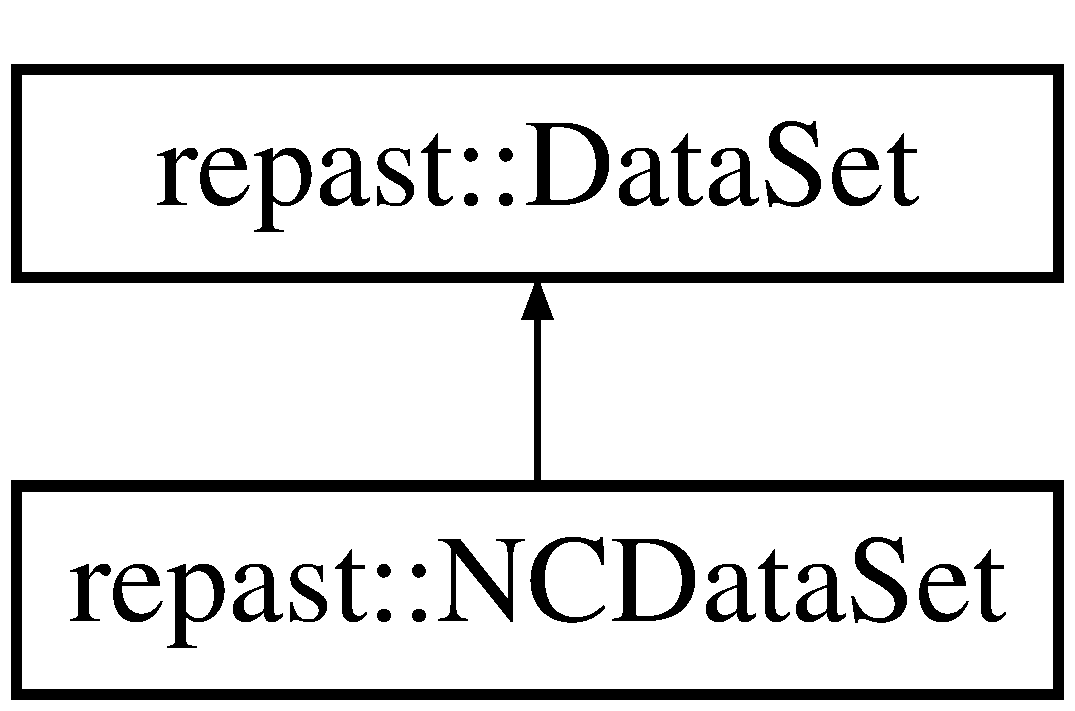
\includegraphics[height=2.000000cm]{classrepast_1_1_n_c_data_set}
\end{center}
\end{figure}
\subsection*{Public Member Functions}
\begin{DoxyCompactItemize}
\item 
\hypertarget{classrepast_1_1_n_c_data_set_a1f4023890763fbfc4323df54d5d90f9e}{void \hyperlink{classrepast_1_1_n_c_data_set_a1f4023890763fbfc4323df54d5d90f9e}{record} ()}\label{classrepast_1_1_n_c_data_set_a1f4023890763fbfc4323df54d5d90f9e}

\begin{DoxyCompactList}\small\item\em Records the data. \end{DoxyCompactList}\item 
\hypertarget{classrepast_1_1_n_c_data_set_a715c1d9a179a2586c42d3b483fa52826}{void \hyperlink{classrepast_1_1_n_c_data_set_a715c1d9a179a2586c42d3b483fa52826}{write} ()}\label{classrepast_1_1_n_c_data_set_a715c1d9a179a2586c42d3b483fa52826}

\begin{DoxyCompactList}\small\item\em Writes the data. \end{DoxyCompactList}\item 
\hypertarget{classrepast_1_1_n_c_data_set_a40f1359629cc1ae4aa974eb52ff8a690}{void \hyperlink{classrepast_1_1_n_c_data_set_a40f1359629cc1ae4aa974eb52ff8a690}{close} ()}\label{classrepast_1_1_n_c_data_set_a40f1359629cc1ae4aa974eb52ff8a690}

\begin{DoxyCompactList}\small\item\em Closes the dataset, after which it must be recreated to be used. \end{DoxyCompactList}\end{DoxyCompactItemize}
\subsection*{Friends}
\begin{DoxyCompactItemize}
\item 
\hypertarget{classrepast_1_1_n_c_data_set_acabe4720b4e1263ea1efb10b32c8adf7}{class {\bfseries N\-C\-Data\-Set\-Builder}}\label{classrepast_1_1_n_c_data_set_acabe4720b4e1263ea1efb10b32c8adf7}

\end{DoxyCompactItemize}


\subsection{Detailed Description}
Provides data recording and writing into a single file in Net\-C\-D\-F format. 

A \hyperlink{classrepast_1_1_n_c_data_set}{N\-C\-Data\-Set} uses rank 0 to write to a single file from multiple pan-\/process data sources. A \hyperlink{classrepast_1_1_n_c_data_set}{N\-C\-Data\-Set} should be built using a \hyperlink{classrepast_1_1_n_c_data_set_builder}{N\-C\-Data\-Set\-Builder}. 

The documentation for this class was generated from the following files\-:\begin{DoxyCompactItemize}
\item 
repast\-\_\-hpc/N\-C\-Data\-Set.\-h\item 
repast\-\_\-hpc/N\-C\-Data\-Set.\-cpp\end{DoxyCompactItemize}

\hypertarget{classrepast_1_1_n_c_data_set_builder}{\section{repast\-:\-:N\-C\-Data\-Set\-Builder Class Reference}
\label{classrepast_1_1_n_c_data_set_builder}\index{repast\-::\-N\-C\-Data\-Set\-Builder@{repast\-::\-N\-C\-Data\-Set\-Builder}}
}


Used to build N\-C\-Data\-Sets to record data in Net\-C\-D\-F format.  




{\ttfamily \#include $<$N\-C\-Data\-Set\-Builder.\-h$>$}

\subsection*{Public Member Functions}
\begin{DoxyCompactItemize}
\item 
\hyperlink{classrepast_1_1_n_c_data_set_builder_a59f6a34ad2c29c55d9d817e1ad24434c}{N\-C\-Data\-Set\-Builder} (std\-::string file, const \hyperlink{classrepast_1_1_schedule}{Schedule} \&schedule)
\begin{DoxyCompactList}\small\item\em Creates an \hyperlink{classrepast_1_1_n_c_data_set_builder}{N\-C\-Data\-Set\-Builder} that will write to the specified file and get its tick counts from the specified schedule. \end{DoxyCompactList}\item 
\hyperlink{classrepast_1_1_n_c_data_set_builder}{N\-C\-Data\-Set\-Builder} \& \hyperlink{classrepast_1_1_n_c_data_set_builder_aafe67957e9e7fd5eb306c351a7f28c54}{add\-Data\-Source} (\hyperlink{classrepast_1_1_n_c_data_source}{N\-C\-Data\-Source} $\ast$source)
\begin{DoxyCompactList}\small\item\em Adds a \hyperlink{classrepast_1_1_n_c_data_source}{N\-C\-Data\-Source} to this \hyperlink{classrepast_1_1_n_c_data_set_builder}{N\-C\-Data\-Set\-Builder}. \end{DoxyCompactList}\item 
\hyperlink{classrepast_1_1_n_c_data_set}{N\-C\-Data\-Set} $\ast$ \hyperlink{classrepast_1_1_n_c_data_set_builder_a6674abbc1f28e0141a6f59a618fd0e62}{create\-Data\-Set} ()
\begin{DoxyCompactList}\small\item\em Creates the \hyperlink{classrepast_1_1_n_c_data_set}{N\-C\-Data\-Set} defined by this \hyperlink{classrepast_1_1_n_c_data_set_builder}{N\-C\-Data\-Set\-Builder}. \end{DoxyCompactList}\end{DoxyCompactItemize}


\subsection{Detailed Description}
Used to build N\-C\-Data\-Sets to record data in Net\-C\-D\-F format. 

Steps for use are\-: 
\begin{DoxyEnumerate}
\item Create a \hyperlink{classrepast_1_1_n_c_data_set_builder}{N\-C\-Data\-Set\-Builder}. 
\item Add N\-C\-Data\-Sources to the builder using the create\-N\-C\-Data\-Source functions. Each Data\-Source defines a variable and where the data for that variable will be retrieved. Recording data on the \hyperlink{classrepast_1_1_n_c_data_set}{N\-C\-Data\-Set} produced by the builder will record this data for each variable. 
\item Call create\-Data\-Set to create the \hyperlink{classrepast_1_1_n_c_data_set}{N\-C\-Data\-Set}. 
\item \hyperlink{classrepast_1_1_schedule}{Schedule} calls to record and write on the \hyperlink{classrepast_1_1_n_c_data_set}{N\-C\-Data\-Set}. 
\end{DoxyEnumerate}

\subsection{Constructor \& Destructor Documentation}
\hypertarget{classrepast_1_1_n_c_data_set_builder_a59f6a34ad2c29c55d9d817e1ad24434c}{\index{repast\-::\-N\-C\-Data\-Set\-Builder@{repast\-::\-N\-C\-Data\-Set\-Builder}!N\-C\-Data\-Set\-Builder@{N\-C\-Data\-Set\-Builder}}
\index{N\-C\-Data\-Set\-Builder@{N\-C\-Data\-Set\-Builder}!repast::NCDataSetBuilder@{repast\-::\-N\-C\-Data\-Set\-Builder}}
\subsubsection[{N\-C\-Data\-Set\-Builder}]{\setlength{\rightskip}{0pt plus 5cm}repast\-::\-N\-C\-Data\-Set\-Builder\-::\-N\-C\-Data\-Set\-Builder (
\begin{DoxyParamCaption}
\item[{std\-::string}]{file, }
\item[{const {\bf Schedule} \&}]{schedule}
\end{DoxyParamCaption}
)}}\label{classrepast_1_1_n_c_data_set_builder_a59f6a34ad2c29c55d9d817e1ad24434c}


Creates an \hyperlink{classrepast_1_1_n_c_data_set_builder}{N\-C\-Data\-Set\-Builder} that will write to the specified file and get its tick counts from the specified schedule. 


\begin{DoxyParams}{Parameters}
{\em file} & the name of the file to write to. Only rank 0 will actually write to this file. \\
\hline
{\em schedule} & the schedule to get tick counts from \\
\hline
\end{DoxyParams}


\subsection{Member Function Documentation}
\hypertarget{classrepast_1_1_n_c_data_set_builder_aafe67957e9e7fd5eb306c351a7f28c54}{\index{repast\-::\-N\-C\-Data\-Set\-Builder@{repast\-::\-N\-C\-Data\-Set\-Builder}!add\-Data\-Source@{add\-Data\-Source}}
\index{add\-Data\-Source@{add\-Data\-Source}!repast::NCDataSetBuilder@{repast\-::\-N\-C\-Data\-Set\-Builder}}
\subsubsection[{add\-Data\-Source}]{\setlength{\rightskip}{0pt plus 5cm}{\bf N\-C\-Data\-Set\-Builder} \& repast\-::\-N\-C\-Data\-Set\-Builder\-::add\-Data\-Source (
\begin{DoxyParamCaption}
\item[{{\bf N\-C\-Data\-Source} $\ast$}]{source}
\end{DoxyParamCaption}
)}}\label{classrepast_1_1_n_c_data_set_builder_aafe67957e9e7fd5eb306c351a7f28c54}


Adds a \hyperlink{classrepast_1_1_n_c_data_source}{N\-C\-Data\-Source} to this \hyperlink{classrepast_1_1_n_c_data_set_builder}{N\-C\-Data\-Set\-Builder}. 

The added \hyperlink{classrepast_1_1_n_c_data_source}{N\-C\-Data\-Source} defines a variable and where the data for that variable will be retrieved. Recording data on the \hyperlink{classrepast_1_1_n_c_data_set}{N\-C\-Data\-Set} produced by this builder will record this data for each variable. \hypertarget{classrepast_1_1_n_c_data_set_builder_a6674abbc1f28e0141a6f59a618fd0e62}{\index{repast\-::\-N\-C\-Data\-Set\-Builder@{repast\-::\-N\-C\-Data\-Set\-Builder}!create\-Data\-Set@{create\-Data\-Set}}
\index{create\-Data\-Set@{create\-Data\-Set}!repast::NCDataSetBuilder@{repast\-::\-N\-C\-Data\-Set\-Builder}}
\subsubsection[{create\-Data\-Set}]{\setlength{\rightskip}{0pt plus 5cm}{\bf N\-C\-Data\-Set} $\ast$ repast\-::\-N\-C\-Data\-Set\-Builder\-::create\-Data\-Set (
\begin{DoxyParamCaption}
{}
\end{DoxyParamCaption}
)}}\label{classrepast_1_1_n_c_data_set_builder_a6674abbc1f28e0141a6f59a618fd0e62}


Creates the \hyperlink{classrepast_1_1_n_c_data_set}{N\-C\-Data\-Set} defined by this \hyperlink{classrepast_1_1_n_c_data_set_builder}{N\-C\-Data\-Set\-Builder}. 

The caller is responsible for properly deleting the returned pointer.

\begin{DoxyReturn}{Returns}
the created \hyperlink{classrepast_1_1_n_c_data_set}{N\-C\-Data\-Set}. 
\end{DoxyReturn}


The documentation for this class was generated from the following files\-:\begin{DoxyCompactItemize}
\item 
repast\-\_\-hpc/N\-C\-Data\-Set\-Builder.\-h\item 
repast\-\_\-hpc/N\-C\-Data\-Set\-Builder.\-cpp\end{DoxyCompactItemize}

\hypertarget{classrepast_1_1_n_c_data_source}{\section{repast\-:\-:N\-C\-Data\-Source Class Reference}
\label{classrepast_1_1_n_c_data_source}\index{repast\-::\-N\-C\-Data\-Source@{repast\-::\-N\-C\-Data\-Source}}
}


Data source used internally by N\-C\-Data\-Sets.  




{\ttfamily \#include $<$N\-C\-Data\-Source.\-h$>$}

Inheritance diagram for repast\-:\-:N\-C\-Data\-Source\-:\begin{figure}[H]
\begin{center}
\leavevmode
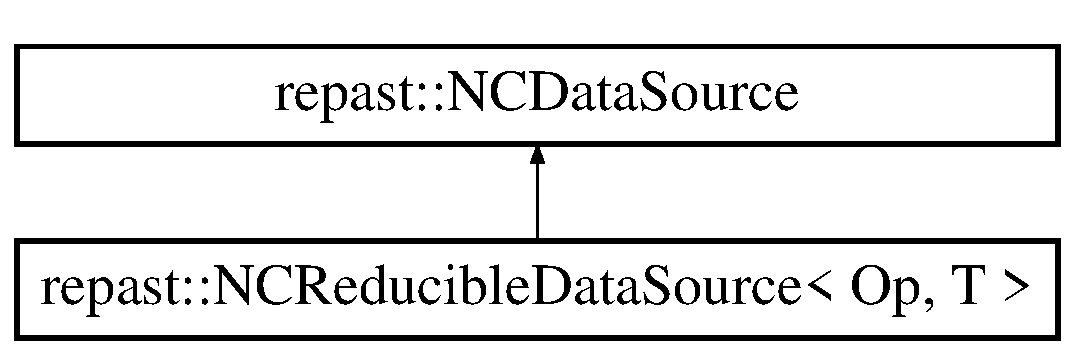
\includegraphics[height=2.000000cm]{classrepast_1_1_n_c_data_source}
\end{center}
\end{figure}
\subsection*{Public Member Functions}
\begin{DoxyCompactItemize}
\item 
\hypertarget{classrepast_1_1_n_c_data_source_a1f7164f8187259412de1bcba13e715f7}{{\bfseries N\-C\-Data\-Source} (std\-::string name)}\label{classrepast_1_1_n_c_data_source_a1f7164f8187259412de1bcba13e715f7}

\item 
\hypertarget{classrepast_1_1_n_c_data_source_a7c698d7661ed5d0c05c47bf9f0fc85f4}{virtual void {\bfseries record} ()=0}\label{classrepast_1_1_n_c_data_source_a7c698d7661ed5d0c05c47bf9f0fc85f4}

\item 
\hypertarget{classrepast_1_1_n_c_data_source_acd388166a86f69d483294a6180659a6c}{virtual void {\bfseries write} (Nc\-Var $\ast$var)=0}\label{classrepast_1_1_n_c_data_source_acd388166a86f69d483294a6180659a6c}

\item 
\hypertarget{classrepast_1_1_n_c_data_source_a63c2afe61362c76b2158a01ff316dc75}{virtual Nc\-Type {\bfseries nc\-Type} ()=0}\label{classrepast_1_1_n_c_data_source_a63c2afe61362c76b2158a01ff316dc75}

\item 
\hypertarget{classrepast_1_1_n_c_data_source_a73dafa85a05b1b8ed5000cc7b288e8e1}{const std\-::string {\bfseries name} () const }\label{classrepast_1_1_n_c_data_source_a73dafa85a05b1b8ed5000cc7b288e8e1}

\end{DoxyCompactItemize}
\subsection*{Protected Attributes}
\begin{DoxyCompactItemize}
\item 
\hypertarget{classrepast_1_1_n_c_data_source_a6bc7455c847f7296f84c85df369b6631}{std\-::string {\bfseries \-\_\-name}}\label{classrepast_1_1_n_c_data_source_a6bc7455c847f7296f84c85df369b6631}

\end{DoxyCompactItemize}


\subsection{Detailed Description}
Data source used internally by N\-C\-Data\-Sets. 

The documentation for this class was generated from the following file\-:\begin{DoxyCompactItemize}
\item 
repast\-\_\-hpc/N\-C\-Data\-Source.\-h\end{DoxyCompactItemize}

\hypertarget{classrepast_1_1_n_c_reducible_data_source}{\section{repast\-:\-:N\-C\-Reducible\-Data\-Source$<$ Op, T $>$ Class Template Reference}
\label{classrepast_1_1_n_c_reducible_data_source}\index{repast\-::\-N\-C\-Reducible\-Data\-Source$<$ Op, T $>$@{repast\-::\-N\-C\-Reducible\-Data\-Source$<$ Op, T $>$}}
}


Source of data and a reduction operation.  




{\ttfamily \#include $<$N\-C\-Reducible\-Data\-Source.\-h$>$}

Inheritance diagram for repast\-:\-:N\-C\-Reducible\-Data\-Source$<$ Op, T $>$\-:\begin{figure}[H]
\begin{center}
\leavevmode
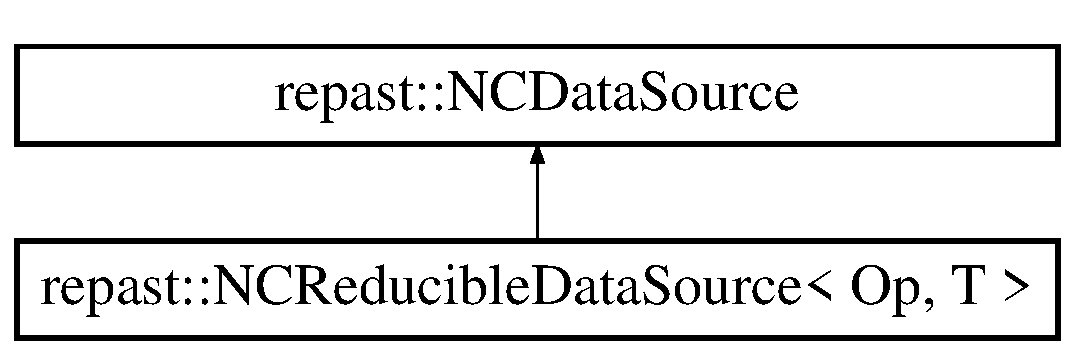
\includegraphics[height=2.000000cm]{classrepast_1_1_n_c_reducible_data_source}
\end{center}
\end{figure}
\subsection*{Public Member Functions}
\begin{DoxyCompactItemize}
\item 
\hypertarget{classrepast_1_1_n_c_reducible_data_source_abb51dc12d9c9b96651098d47f775f589}{{\bfseries N\-C\-Reducible\-Data\-Source} (std\-::string name, \hyperlink{classrepast_1_1_t_data_source}{T\-Data\-Source}$<$ T $>$ $\ast$data\-Source, Op op)}\label{classrepast_1_1_n_c_reducible_data_source_abb51dc12d9c9b96651098d47f775f589}

\item 
\hypertarget{classrepast_1_1_n_c_reducible_data_source_a232af9bb522eb699fdb9c20e14304588}{virtual Nc\-Type {\bfseries nc\-Type} ()}\label{classrepast_1_1_n_c_reducible_data_source_a232af9bb522eb699fdb9c20e14304588}

\item 
\hypertarget{classrepast_1_1_n_c_reducible_data_source_a3046c509fcffa8bef784ab0152c07e4a}{virtual void {\bfseries record} ()}\label{classrepast_1_1_n_c_reducible_data_source_a3046c509fcffa8bef784ab0152c07e4a}

\item 
\hypertarget{classrepast_1_1_n_c_reducible_data_source_a78425c8622a728038e7b15486445b488}{virtual void {\bfseries write} (Nc\-Var $\ast$var)}\label{classrepast_1_1_n_c_reducible_data_source_a78425c8622a728038e7b15486445b488}

\end{DoxyCompactItemize}
\subsection*{Protected Attributes}
\begin{DoxyCompactItemize}
\item 
\hypertarget{classrepast_1_1_n_c_reducible_data_source_aa5cd25f8ad028a775dc7627c5c91587d}{Op {\bfseries op\-\_\-}}\label{classrepast_1_1_n_c_reducible_data_source_aa5cd25f8ad028a775dc7627c5c91587d}

\item 
\hypertarget{classrepast_1_1_n_c_reducible_data_source_a9685203ae48080b54fa0203e891b54ae}{std\-::vector$<$ T $>$ {\bfseries data}}\label{classrepast_1_1_n_c_reducible_data_source_a9685203ae48080b54fa0203e891b54ae}

\item 
\hypertarget{classrepast_1_1_n_c_reducible_data_source_a5b8b75d2e197c52368b4ccc81f71ed90}{\hyperlink{classrepast_1_1_t_data_source}{T\-Data\-Source}$<$ T $>$ $\ast$ {\bfseries data\-Source\-\_\-}}\label{classrepast_1_1_n_c_reducible_data_source_a5b8b75d2e197c52368b4ccc81f71ed90}

\item 
\hypertarget{classrepast_1_1_n_c_reducible_data_source_a02d3aaeda5a9d70dc599da7b01401668}{int {\bfseries rank}}\label{classrepast_1_1_n_c_reducible_data_source_a02d3aaeda5a9d70dc599da7b01401668}

\item 
\hypertarget{classrepast_1_1_n_c_reducible_data_source_a4a94e07fac10264e228eef6a6f25de83}{int {\bfseries start}}\label{classrepast_1_1_n_c_reducible_data_source_a4a94e07fac10264e228eef6a6f25de83}

\end{DoxyCompactItemize}


\subsection{Detailed Description}
\subsubsection*{template$<$typename Op, typename T$>$class repast\-::\-N\-C\-Reducible\-Data\-Source$<$ Op, T $>$}

Source of data and a reduction operation. 

Used internally by a \hyperlink{classrepast_1_1_n_c_data_set}{N\-C\-Data\-Set} to store the data sources. their associated ops etc. 

The documentation for this class was generated from the following file\-:\begin{DoxyCompactItemize}
\item 
repast\-\_\-hpc/N\-C\-Reducible\-Data\-Source.\-h\end{DoxyCompactItemize}

\hypertarget{structrepast_1_1_nc_type_trait}{\section{repast\-:\-:Nc\-Type\-Trait$<$ T $>$ Struct Template Reference}
\label{structrepast_1_1_nc_type_trait}\index{repast\-::\-Nc\-Type\-Trait$<$ T $>$@{repast\-::\-Nc\-Type\-Trait$<$ T $>$}}
}


Base class for specialized int and double Nc\-Type classes.  




{\ttfamily \#include $<$N\-C\-Data\-Source.\-h$>$}



\subsection{Detailed Description}
\subsubsection*{template$<$typename T$>$struct repast\-::\-Nc\-Type\-Trait$<$ T $>$}

Base class for specialized int and double Nc\-Type classes. 

The documentation for this struct was generated from the following file\-:\begin{DoxyCompactItemize}
\item 
repast\-\_\-hpc/N\-C\-Data\-Source.\-h\end{DoxyCompactItemize}

\hypertarget{structrepast_1_1_nc_type_trait_3_01double_01_4}{\section{repast\-:\-:Nc\-Type\-Trait$<$ double $>$ Struct Template Reference}
\label{structrepast_1_1_nc_type_trait_3_01double_01_4}\index{repast\-::\-Nc\-Type\-Trait$<$ double $>$@{repast\-::\-Nc\-Type\-Trait$<$ double $>$}}
}


Used for converting to Net\-C\-D\-F Data, double type.  




{\ttfamily \#include $<$N\-C\-Data\-Source.\-h$>$}

\subsection*{Static Public Attributes}
\begin{DoxyCompactItemize}
\item 
\hypertarget{structrepast_1_1_nc_type_trait_3_01double_01_4_a6cfe5fde4c4ad6e3c0d0bddb53642238}{static const Nc\-Type {\bfseries type} = nc\-Double}\label{structrepast_1_1_nc_type_trait_3_01double_01_4_a6cfe5fde4c4ad6e3c0d0bddb53642238}

\end{DoxyCompactItemize}


\subsection{Detailed Description}
\subsubsection*{template$<$$>$struct repast\-::\-Nc\-Type\-Trait$<$ double $>$}

Used for converting to Net\-C\-D\-F Data, double type. 

The documentation for this struct was generated from the following file\-:\begin{DoxyCompactItemize}
\item 
repast\-\_\-hpc/N\-C\-Data\-Source.\-h\end{DoxyCompactItemize}

\hypertarget{structrepast_1_1_nc_type_trait_3_01int_01_4}{\section{repast\-:\-:Nc\-Type\-Trait$<$ int $>$ Struct Template Reference}
\label{structrepast_1_1_nc_type_trait_3_01int_01_4}\index{repast\-::\-Nc\-Type\-Trait$<$ int $>$@{repast\-::\-Nc\-Type\-Trait$<$ int $>$}}
}


Used for converting to Net\-C\-D\-F Data, int type.  




{\ttfamily \#include $<$N\-C\-Data\-Source.\-h$>$}

\subsection*{Static Public Attributes}
\begin{DoxyCompactItemize}
\item 
\hypertarget{structrepast_1_1_nc_type_trait_3_01int_01_4_a561856ea039727017e32a5d1313fad5b}{static const Nc\-Type {\bfseries type} = nc\-Int}\label{structrepast_1_1_nc_type_trait_3_01int_01_4_a561856ea039727017e32a5d1313fad5b}

\end{DoxyCompactItemize}


\subsection{Detailed Description}
\subsubsection*{template$<$$>$struct repast\-::\-Nc\-Type\-Trait$<$ int $>$}

Used for converting to Net\-C\-D\-F Data, int type. 

The documentation for this struct was generated from the following file\-:\begin{DoxyCompactItemize}
\item 
repast\-\_\-hpc/N\-C\-Data\-Source.\-h\end{DoxyCompactItemize}

\hypertarget{classrepast_1_1_neighbor}{\section{repast\-:\-:Neighbor Class Reference}
\label{classrepast_1_1_neighbor}\index{repast\-::\-Neighbor@{repast\-::\-Neighbor}}
}


Contains the rank and boundaries of a semantically adjacent process (that is, a process that manages the space that is adjacent to the simulation space managed by this process).  




{\ttfamily \#include $<$Shared\-Base\-Grid.\-h$>$}

\subsection*{Public Member Functions}
\begin{DoxyCompactItemize}
\item 
\hypertarget{classrepast_1_1_neighbor_a7063a662d4342a523b2716ae9100da67}{{\bfseries Neighbor} (int rank, \hyperlink{classrepast_1_1_grid_dimensions}{Grid\-Dimensions} bounds)}\label{classrepast_1_1_neighbor_a7063a662d4342a523b2716ae9100da67}

\item 
\hypertarget{classrepast_1_1_neighbor_a09114073766153e1a5e596fd0eba0734}{int {\bfseries rank} () const }\label{classrepast_1_1_neighbor_a09114073766153e1a5e596fd0eba0734}

\item 
\hypertarget{classrepast_1_1_neighbor_ab49a3e501a9a6765bde278c48fe41ae0}{\hyperlink{classrepast_1_1_grid_dimensions}{Grid\-Dimensions} {\bfseries bounds} () const }\label{classrepast_1_1_neighbor_ab49a3e501a9a6765bde278c48fe41ae0}

\end{DoxyCompactItemize}


\subsection{Detailed Description}
Contains the rank and boundaries of a semantically adjacent process (that is, a process that manages the space that is adjacent to the simulation space managed by this process). 

The documentation for this class was generated from the following files\-:\begin{DoxyCompactItemize}
\item 
repast\-\_\-hpc/Shared\-Base\-Grid.\-h\item 
repast\-\_\-hpc/Shared\-Base\-Grid.\-cpp\end{DoxyCompactItemize}

\hypertarget{classrepast_1_1_neighbors}{\section{repast\-:\-:Neighbors Class Reference}
\label{classrepast_1_1_neighbors}\index{repast\-::\-Neighbors@{repast\-::\-Neighbors}}
}


Provides lookup of grid topology process neighbors given a point in the pan process grid.  




{\ttfamily \#include $<$Shared\-Base\-Grid.\-h$>$}

\subsection*{Public Types}
\begin{DoxyCompactItemize}
\item 
enum \hyperlink{classrepast_1_1_neighbors_a7a695a73b614b849f12fd943329b8bdc}{Location} \{ \\*
{\bfseries E}, 
{\bfseries W}, 
{\bfseries N}, 
{\bfseries S}, 
\\*
{\bfseries N\-E}, 
{\bfseries N\-W}, 
{\bfseries S\-E}, 
{\bfseries S\-W}
 \}
\begin{DoxyCompactList}\small\item\em Describes the relative location of grid topology process neighbors. \end{DoxyCompactList}\end{DoxyCompactItemize}
\subsection*{Public Member Functions}
\begin{DoxyCompactItemize}
\item 
\hypertarget{classrepast_1_1_neighbors_acebe1c38c1b9a6492c2bd819aa315640}{void \hyperlink{classrepast_1_1_neighbors_acebe1c38c1b9a6492c2bd819aa315640}{add\-Neighbor} (\hyperlink{classrepast_1_1_neighbor}{Neighbor} $\ast$ngh, \hyperlink{classrepast_1_1_neighbors_a7a695a73b614b849f12fd943329b8bdc}{Neighbors\-::\-Location} location)}\label{classrepast_1_1_neighbors_acebe1c38c1b9a6492c2bd819aa315640}

\begin{DoxyCompactList}\small\item\em Adds a neighbor at the specified location. \end{DoxyCompactList}\item 
\hyperlink{classrepast_1_1_neighbor}{Neighbor} $\ast$ \hyperlink{classrepast_1_1_neighbors_adbcad09f1909177b08c195f64b818c85}{neighbor} (\hyperlink{classrepast_1_1_neighbors_a7a695a73b614b849f12fd943329b8bdc}{Neighbors\-::\-Location} location) const 
\begin{DoxyCompactList}\small\item\em Gets the neighbor at the specified location. \end{DoxyCompactList}\item 
\hyperlink{classrepast_1_1_neighbor}{Neighbor} $\ast$ \hyperlink{classrepast_1_1_neighbors_a745a848c9e0bdc4270dca7cb7d232259}{find\-Neighbor} (const std\-::vector$<$ int $>$ \&pt)
\begin{DoxyCompactList}\small\item\em Finds the neighbor that contains the specified point. \end{DoxyCompactList}\item 
\hyperlink{classrepast_1_1_neighbor}{Neighbor} $\ast$ \hyperlink{classrepast_1_1_neighbors_a6ce8456088582c39eb99d9497e2f4ea0}{find\-Neighbor} (const std\-::vector$<$ double $>$ \&pt)
\begin{DoxyCompactList}\small\item\em Finds the neighbor that contains the specified point. \end{DoxyCompactList}\item 
\hypertarget{classrepast_1_1_neighbors_a51169973f80e7b98147aefd15a217fa9}{void {\bfseries get\-Neighbor\-Ranks} (std\-::set$<$ int $>$ \&ranks)}\label{classrepast_1_1_neighbors_a51169973f80e7b98147aefd15a217fa9}

\end{DoxyCompactItemize}
\subsection*{Static Public Attributes}
\begin{DoxyCompactItemize}
\item 
\hypertarget{classrepast_1_1_neighbors_a906f5117fa96c4402fa39878340fed95}{static const int {\bfseries L\-O\-C\-A\-T\-I\-O\-N\-\_\-\-S\-I\-Z\-E} = 8}\label{classrepast_1_1_neighbors_a906f5117fa96c4402fa39878340fed95}

\end{DoxyCompactItemize}
\subsection*{Friends}
\begin{DoxyCompactItemize}
\item 
\hypertarget{classrepast_1_1_neighbors_a8d0ac1cbe643f03e741e0747cb3931a2}{std\-::ostream \& {\bfseries operator$<$$<$} (std\-::ostream \&os, const \hyperlink{classrepast_1_1_neighbors}{Neighbors} \&nghs)}\label{classrepast_1_1_neighbors_a8d0ac1cbe643f03e741e0747cb3931a2}

\end{DoxyCompactItemize}


\subsection{Detailed Description}
Provides lookup of grid topology process neighbors given a point in the pan process grid. 

\subsection{Member Function Documentation}
\hypertarget{classrepast_1_1_neighbors_a745a848c9e0bdc4270dca7cb7d232259}{\index{repast\-::\-Neighbors@{repast\-::\-Neighbors}!find\-Neighbor@{find\-Neighbor}}
\index{find\-Neighbor@{find\-Neighbor}!repast::Neighbors@{repast\-::\-Neighbors}}
\subsubsection[{find\-Neighbor}]{\setlength{\rightskip}{0pt plus 5cm}{\bf Neighbor} $\ast$ repast\-::\-Neighbors\-::find\-Neighbor (
\begin{DoxyParamCaption}
\item[{const std\-::vector$<$ int $>$ \&}]{pt}
\end{DoxyParamCaption}
)}}\label{classrepast_1_1_neighbors_a745a848c9e0bdc4270dca7cb7d232259}


Finds the neighbor that contains the specified point. 

\begin{DoxyReturn}{Returns}
the found neighbor 
\end{DoxyReturn}
\hypertarget{classrepast_1_1_neighbors_a6ce8456088582c39eb99d9497e2f4ea0}{\index{repast\-::\-Neighbors@{repast\-::\-Neighbors}!find\-Neighbor@{find\-Neighbor}}
\index{find\-Neighbor@{find\-Neighbor}!repast::Neighbors@{repast\-::\-Neighbors}}
\subsubsection[{find\-Neighbor}]{\setlength{\rightskip}{0pt plus 5cm}{\bf Neighbor} $\ast$ repast\-::\-Neighbors\-::find\-Neighbor (
\begin{DoxyParamCaption}
\item[{const std\-::vector$<$ double $>$ \&}]{pt}
\end{DoxyParamCaption}
)}}\label{classrepast_1_1_neighbors_a6ce8456088582c39eb99d9497e2f4ea0}


Finds the neighbor that contains the specified point. 

\begin{DoxyReturn}{Returns}
the found neighbor 
\end{DoxyReturn}
\hypertarget{classrepast_1_1_neighbors_adbcad09f1909177b08c195f64b818c85}{\index{repast\-::\-Neighbors@{repast\-::\-Neighbors}!neighbor@{neighbor}}
\index{neighbor@{neighbor}!repast::Neighbors@{repast\-::\-Neighbors}}
\subsubsection[{neighbor}]{\setlength{\rightskip}{0pt plus 5cm}{\bf Neighbor} $\ast$ repast\-::\-Neighbors\-::neighbor (
\begin{DoxyParamCaption}
\item[{{\bf Neighbors\-::\-Location}}]{location}
\end{DoxyParamCaption}
) const}}\label{classrepast_1_1_neighbors_adbcad09f1909177b08c195f64b818c85}


Gets the neighbor at the specified location. 


\begin{DoxyParams}{Parameters}
{\em location} & the location of the neighbor. \\
\hline
\end{DoxyParams}


The documentation for this class was generated from the following files\-:\begin{DoxyCompactItemize}
\item 
repast\-\_\-hpc/Shared\-Base\-Grid.\-h\item 
repast\-\_\-hpc/Shared\-Base\-Grid.\-cpp\end{DoxyCompactItemize}

\hypertarget{structrepast_1_1_node_getter}{\section{repast\-:\-:Node\-Getter$<$ V, E $>$ Struct Template Reference}
\label{structrepast_1_1_node_getter}\index{repast\-::\-Node\-Getter$<$ V, E $>$@{repast\-::\-Node\-Getter$<$ V, E $>$}}
}


Unary function used in the transform\-\_\-iterator that allows an iterator over the vertex map to return the node.  




{\ttfamily \#include $<$Vertex.\-h$>$}

Inheritance diagram for repast\-:\-:Node\-Getter$<$ V, E $>$\-:\begin{figure}[H]
\begin{center}
\leavevmode
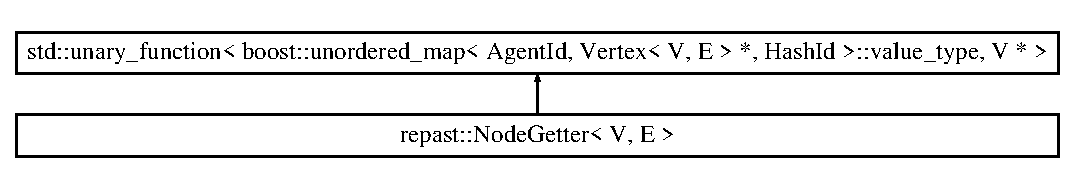
\includegraphics[height=1.876047cm]{structrepast_1_1_node_getter}
\end{center}
\end{figure}
\subsection*{Public Member Functions}
\begin{DoxyCompactItemize}
\item 
\hypertarget{structrepast_1_1_node_getter_af738a8ad2b713303a0e95132588864fb}{V $\ast$ {\bfseries operator()} (const typename boost\-::unordered\-\_\-map$<$ \hyperlink{classrepast_1_1_agent_id}{Agent\-Id}, \hyperlink{classrepast_1_1_vertex}{Vertex}$<$ V, E $>$ $\ast$, \hyperlink{structrepast_1_1_hash_id}{Hash\-Id} $>$\-::value\-\_\-type \&value) const }\label{structrepast_1_1_node_getter_af738a8ad2b713303a0e95132588864fb}

\end{DoxyCompactItemize}


\subsection{Detailed Description}
\subsubsection*{template$<$typename V, typename E$>$struct repast\-::\-Node\-Getter$<$ V, E $>$}

Unary function used in the transform\-\_\-iterator that allows an iterator over the vertex map to return the node. 

The documentation for this struct was generated from the following file\-:\begin{DoxyCompactItemize}
\item 
repast\-\_\-hpc/Vertex.\-h\end{DoxyCompactItemize}

\hypertarget{classrepast_1_1_number_generator}{\section{repast\-:\-:Number\-Generator Class Reference}
\label{classrepast_1_1_number_generator}\index{repast\-::\-Number\-Generator@{repast\-::\-Number\-Generator}}
}


Number generator interface.  




{\ttfamily \#include $<$Random.\-h$>$}

Inheritance diagram for repast\-:\-:Number\-Generator\-:\begin{figure}[H]
\begin{center}
\leavevmode
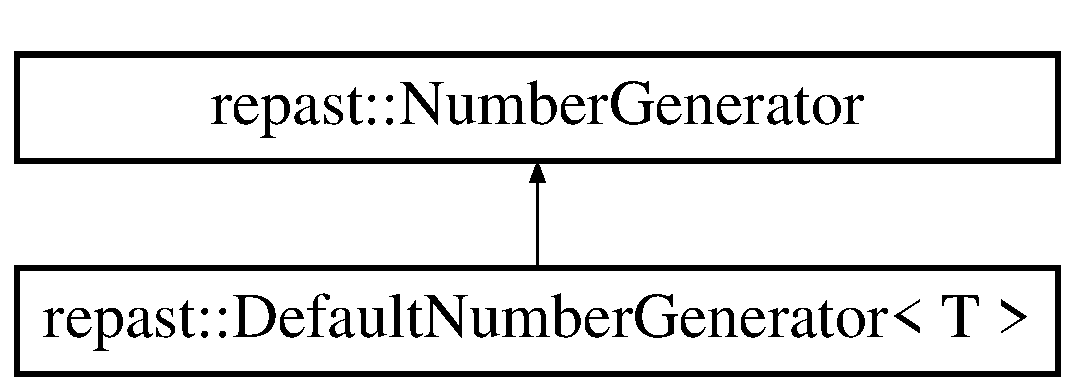
\includegraphics[height=2.000000cm]{classrepast_1_1_number_generator}
\end{center}
\end{figure}
\subsection*{Public Member Functions}
\begin{DoxyCompactItemize}
\item 
\hypertarget{classrepast_1_1_number_generator_a98d94cf82a5283ff29d0df69b1b2f67c}{virtual double \hyperlink{classrepast_1_1_number_generator_a98d94cf82a5283ff29d0df69b1b2f67c}{next} ()=0}\label{classrepast_1_1_number_generator_a98d94cf82a5283ff29d0df69b1b2f67c}

\begin{DoxyCompactList}\small\item\em Gets the \char`\"{}next\char`\"{} number from this Number Generator. \end{DoxyCompactList}\end{DoxyCompactItemize}


\subsection{Detailed Description}
Number generator interface. 

The documentation for this class was generated from the following file\-:\begin{DoxyCompactItemize}
\item 
repast\-\_\-hpc/Random.\-h\end{DoxyCompactItemize}

\hypertarget{classrepast_1_1_one_time_event}{\section{repast\-:\-:One\-Time\-Event Class Reference}
\label{classrepast_1_1_one_time_event}\index{repast\-::\-One\-Time\-Event@{repast\-::\-One\-Time\-Event}}
}


\hyperlink{classrepast_1_1_scheduled_event}{Scheduled\-Event} that will only execute only once.  




{\ttfamily \#include $<$Schedule.\-h$>$}

Inheritance diagram for repast\-:\-:One\-Time\-Event\-:\begin{figure}[H]
\begin{center}
\leavevmode
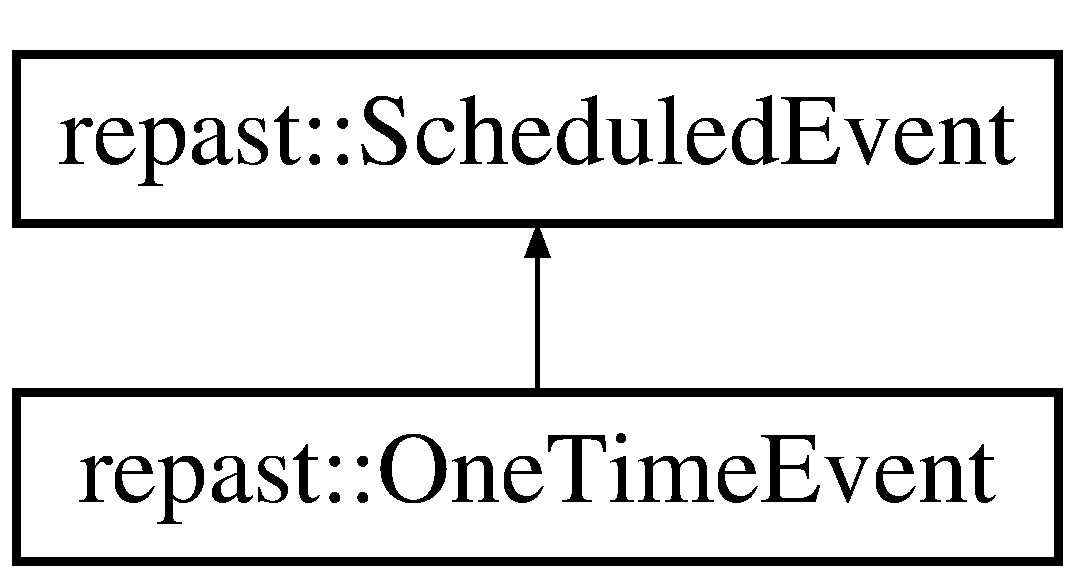
\includegraphics[height=2.000000cm]{classrepast_1_1_one_time_event}
\end{center}
\end{figure}
\subsection*{Public Member Functions}
\begin{DoxyCompactItemize}
\item 
\hypertarget{classrepast_1_1_one_time_event_aa5e82b975901d00868417645b66bbc71}{{\bfseries One\-Time\-Event} (double, \hyperlink{classrepast_1_1_repast_event}{Repast\-Event} $\ast$)}\label{classrepast_1_1_one_time_event_aa5e82b975901d00868417645b66bbc71}

\item 
\hypertarget{classrepast_1_1_one_time_event_a015c78426a9c7bc7de042d66b4387ecb}{virtual bool \hyperlink{classrepast_1_1_one_time_event_a015c78426a9c7bc7de042d66b4387ecb}{reschedule} (std\-::priority\-\_\-queue$<$ \hyperlink{classrepast_1_1_scheduled_event}{Scheduled\-Event} $\ast$, std\-::vector$<$ \hyperlink{classrepast_1_1_scheduled_event}{Scheduled\-Event} $\ast$ $>$, \hyperlink{classrepast_1_1_event_compare}{Event\-Compare} $>$ \&)}\label{classrepast_1_1_one_time_event_a015c78426a9c7bc7de042d66b4387ecb}

\begin{DoxyCompactList}\small\item\em Always returns false, as it does not reschedule itself. \end{DoxyCompactList}\end{DoxyCompactItemize}
\subsection*{Additional Inherited Members}


\subsection{Detailed Description}
\hyperlink{classrepast_1_1_scheduled_event}{Scheduled\-Event} that will only execute only once. 

The documentation for this class was generated from the following files\-:\begin{DoxyCompactItemize}
\item 
repast\-\_\-hpc/Schedule.\-h\item 
repast\-\_\-hpc/Schedule.\-cpp\end{DoxyCompactItemize}

\hypertarget{classrepast_1_1_point}{\section{repast\-:\-:Point$<$ T $>$ Class Template Reference}
\label{classrepast_1_1_point}\index{repast\-::\-Point$<$ T $>$@{repast\-::\-Point$<$ T $>$}}
}


A N-\/dimensional \hyperlink{classrepast_1_1_point}{Point} representation.  




{\ttfamily \#include $<$Point.\-h$>$}

\subsection*{Public Types}
\begin{DoxyCompactItemize}
\item 
\hypertarget{classrepast_1_1_point_a5b7b0786c5ac836e6ddfcda1dec866dc}{typedef std\-::vector$<$ T $>$\\*
\-::const\-\_\-iterator {\bfseries const\-\_\-iterator}}\label{classrepast_1_1_point_a5b7b0786c5ac836e6ddfcda1dec866dc}

\end{DoxyCompactItemize}
\subsection*{Public Member Functions}
\begin{DoxyCompactItemize}
\item 
\hyperlink{classrepast_1_1_point_ab873dcd5fc9b62c27f9f75a602077d0b}{Point} (T x)
\begin{DoxyCompactList}\small\item\em Creates a one dimensional point with the specified value. \end{DoxyCompactList}\item 
\hyperlink{classrepast_1_1_point_abed6f095fe52bf4c72b3142563db9bc7}{Point} (T x, T y)
\begin{DoxyCompactList}\small\item\em Creates a two dimensional point with the specified values. \end{DoxyCompactList}\item 
\hyperlink{classrepast_1_1_point_a05d9583817d89b4347ab7d764212a1b1}{Point} (T x, T y, T z)
\begin{DoxyCompactList}\small\item\em Creates a three dimensional point with the specified values. \end{DoxyCompactList}\item 
\hyperlink{classrepast_1_1_point_a9dadb20bf3ca390851a8df68850d2be5}{Point} (std\-::vector$<$ T $>$ coordinates)
\begin{DoxyCompactList}\small\item\em Creates a multi-\/dimensional point with the specified values. \end{DoxyCompactList}\item 
T \hyperlink{classrepast_1_1_point_af985d58e3c8ccd00e54dd46fc71b41b2}{get\-X} () const 
\begin{DoxyCompactList}\small\item\em Gets the x coordinate of the point. \end{DoxyCompactList}\item 
T \hyperlink{classrepast_1_1_point_ac4c09bef3c9be3b69432da55da2c7c57}{get\-Y} () const 
\begin{DoxyCompactList}\small\item\em Gets the y coordinate of the point. \end{DoxyCompactList}\item 
T \hyperlink{classrepast_1_1_point_a2abcd532878f05b30961306b790664e3}{get\-Z} () const 
\begin{DoxyCompactList}\small\item\em Gets the z coordinate of the point. \end{DoxyCompactList}\item 
T \hyperlink{classrepast_1_1_point_a22a3eab287df785225791d1d1a75c89c}{get\-Coordinate} (int coord\-Index) const 
\begin{DoxyCompactList}\small\item\em Gets the coodinate of the point in the specified dimension. \end{DoxyCompactList}\item 
void \hyperlink{classrepast_1_1_point_a8b7e9df41c4aa2d7387138a404fc3982}{add} (const \hyperlink{classrepast_1_1_point}{Point}$<$ T $>$ \&pt)
\begin{DoxyCompactList}\small\item\em Adds the specified Grid\-Point to this Grid\-Point. \end{DoxyCompactList}\item 
size\-\_\-t \hyperlink{classrepast_1_1_point_ac872326f55cdbfa5106d430bea6d959c}{dimension\-Count} () const 
\begin{DoxyCompactList}\small\item\em Gets the number of dimensions of this point. \end{DoxyCompactList}\item 
const T \& \hyperlink{classrepast_1_1_point_a0ac1a3a42fc61f022d706a05238e98f1}{operator\mbox{[}$\,$\mbox{]}} (size\-\_\-t index) const 
\begin{DoxyCompactList}\small\item\em Gets the coordinate value at the specified index. \end{DoxyCompactList}\item 
T \& \hyperlink{classrepast_1_1_point_a1214b8f5293b222ff2bb115fe30127c2}{operator\mbox{[}$\,$\mbox{]}} (size\-\_\-t index)
\begin{DoxyCompactList}\small\item\em Gets the coordinate value at the specified index. \end{DoxyCompactList}\item 
const std\-::vector$<$ T $>$ \& \hyperlink{classrepast_1_1_point_ac821ebc5c69d6bf8ab132babddcbb864}{coords} () const 
\begin{DoxyCompactList}\small\item\em Gets the coordinates of this point as a vector. \end{DoxyCompactList}\item 
const\-\_\-iterator \hyperlink{classrepast_1_1_point_aec55ad9f0415bfa707daf019328514ed}{begin} () const 
\begin{DoxyCompactList}\small\item\em Gets the start of an iterator over the coordinates of this point. \end{DoxyCompactList}\item 
const\-\_\-iterator \hyperlink{classrepast_1_1_point_a4859ae010bfd59c8c37283d8af58b160}{end} () const 
\begin{DoxyCompactList}\small\item\em Gets the end of an iterator over the coordinates of this point. \end{DoxyCompactList}\item 
void \hyperlink{classrepast_1_1_point_a6c7ba452e7c41d28216ed7a7abfb623a}{copy} (std\-::vector$<$ T $>$ \&out) const 
\begin{DoxyCompactList}\small\item\em Copies the point into the specified vector. \end{DoxyCompactList}\end{DoxyCompactItemize}
\subsection*{Friends}
\begin{DoxyCompactItemize}
\item 
\hypertarget{classrepast_1_1_point_a75395e59eeb036931f89fc247e44910e}{struct {\bfseries Hash\-Grid\-Point$<$ T $>$}}\label{classrepast_1_1_point_a75395e59eeb036931f89fc247e44910e}

\item 
\hypertarget{classrepast_1_1_point_ac98d07dd8f7b70e16ccb9a01abf56b9c}{class {\bfseries boost\-::serialization\-::access}}\label{classrepast_1_1_point_ac98d07dd8f7b70e16ccb9a01abf56b9c}

\item 
\hypertarget{classrepast_1_1_point_a2438176b2bab962e952bbeb309af3497}{bool {\bfseries operator==} (const \hyperlink{classrepast_1_1_point}{Point}$<$ T $>$ \&one, const \hyperlink{classrepast_1_1_point}{Point}$<$ T $>$ \&two)}\label{classrepast_1_1_point_a2438176b2bab962e952bbeb309af3497}

\item 
\hypertarget{classrepast_1_1_point_abf6f92c0466e14e91f78c562ea44cfef}{std\-::ostream \& {\bfseries operator$<$$<$} (std\-::ostream \&os, const \hyperlink{classrepast_1_1_point}{Point}$<$ T $>$ \&pt)}\label{classrepast_1_1_point_abf6f92c0466e14e91f78c562ea44cfef}

\end{DoxyCompactItemize}


\subsection{Detailed Description}
\subsubsection*{template$<$typename T$>$class repast\-::\-Point$<$ T $>$}

A N-\/dimensional \hyperlink{classrepast_1_1_point}{Point} representation. 

N dimensional point for addressing matrix locations.


\begin{DoxyParams}{Parameters}
{\em T} & a numeric type. In repast and relogo these are limited to int and double. \\
\hline
\end{DoxyParams}


\subsection{Constructor \& Destructor Documentation}
\hypertarget{classrepast_1_1_point_ab873dcd5fc9b62c27f9f75a602077d0b}{\index{repast\-::\-Point@{repast\-::\-Point}!Point@{Point}}
\index{Point@{Point}!repast::Point@{repast\-::\-Point}}
\subsubsection[{Point}]{\setlength{\rightskip}{0pt plus 5cm}template$<$typename T$>$ {\bf repast\-::\-Point}$<$ T $>$\-::{\bf Point} (
\begin{DoxyParamCaption}
\item[{T}]{x}
\end{DoxyParamCaption}
)\hspace{0.3cm}{\ttfamily [explicit]}}}\label{classrepast_1_1_point_ab873dcd5fc9b62c27f9f75a602077d0b}


Creates a one dimensional point with the specified value. 


\begin{DoxyParams}{Parameters}
{\em x} & the x coordinate of the point \\
\hline
\end{DoxyParams}
\hypertarget{classrepast_1_1_point_abed6f095fe52bf4c72b3142563db9bc7}{\index{repast\-::\-Point@{repast\-::\-Point}!Point@{Point}}
\index{Point@{Point}!repast::Point@{repast\-::\-Point}}
\subsubsection[{Point}]{\setlength{\rightskip}{0pt plus 5cm}template$<$typename T$>$ {\bf repast\-::\-Point}$<$ T $>$\-::{\bf Point} (
\begin{DoxyParamCaption}
\item[{T}]{x, }
\item[{T}]{y}
\end{DoxyParamCaption}
)}}\label{classrepast_1_1_point_abed6f095fe52bf4c72b3142563db9bc7}


Creates a two dimensional point with the specified values. 


\begin{DoxyParams}{Parameters}
{\em x} & the x coordinate of the point \\
\hline
{\em y} & the y coordinate of the point \\
\hline
\end{DoxyParams}
\hypertarget{classrepast_1_1_point_a05d9583817d89b4347ab7d764212a1b1}{\index{repast\-::\-Point@{repast\-::\-Point}!Point@{Point}}
\index{Point@{Point}!repast::Point@{repast\-::\-Point}}
\subsubsection[{Point}]{\setlength{\rightskip}{0pt plus 5cm}template$<$typename T$>$ {\bf repast\-::\-Point}$<$ T $>$\-::{\bf Point} (
\begin{DoxyParamCaption}
\item[{T}]{x, }
\item[{T}]{y, }
\item[{T}]{z}
\end{DoxyParamCaption}
)}}\label{classrepast_1_1_point_a05d9583817d89b4347ab7d764212a1b1}


Creates a three dimensional point with the specified values. 


\begin{DoxyParams}{Parameters}
{\em x} & the x coordinate of the point \\
\hline
{\em y} & the y coordinate of the point \\
\hline
{\em z} & the z coordinate of the point \\
\hline
\end{DoxyParams}
\hypertarget{classrepast_1_1_point_a9dadb20bf3ca390851a8df68850d2be5}{\index{repast\-::\-Point@{repast\-::\-Point}!Point@{Point}}
\index{Point@{Point}!repast::Point@{repast\-::\-Point}}
\subsubsection[{Point}]{\setlength{\rightskip}{0pt plus 5cm}template$<$typename T$>$ {\bf repast\-::\-Point}$<$ T $>$\-::{\bf Point} (
\begin{DoxyParamCaption}
\item[{std\-::vector$<$ T $>$}]{coordinates}
\end{DoxyParamCaption}
)}}\label{classrepast_1_1_point_a9dadb20bf3ca390851a8df68850d2be5}


Creates a multi-\/dimensional point with the specified values. 


\begin{DoxyParams}{Parameters}
{\em coordinates} & the coordinate values of the point. The first element will be x, the second y and so on. \\
\hline
\end{DoxyParams}


\subsection{Member Function Documentation}
\hypertarget{classrepast_1_1_point_a8b7e9df41c4aa2d7387138a404fc3982}{\index{repast\-::\-Point@{repast\-::\-Point}!add@{add}}
\index{add@{add}!repast::Point@{repast\-::\-Point}}
\subsubsection[{add}]{\setlength{\rightskip}{0pt plus 5cm}template$<$typename T$>$ void {\bf repast\-::\-Point}$<$ T $>$\-::add (
\begin{DoxyParamCaption}
\item[{const {\bf Point}$<$ T $>$ \&}]{pt}
\end{DoxyParamCaption}
)}}\label{classrepast_1_1_point_a8b7e9df41c4aa2d7387138a404fc3982}


Adds the specified Grid\-Point to this Grid\-Point. 

This Grid\-Point contains the result.


\begin{DoxyExceptions}{Exceptions}
{\em invalid\-\_\-argument} & exception if the pt doesn't have the same number of dimensions as this Grid\-Point. \\
\hline
\end{DoxyExceptions}
\hypertarget{classrepast_1_1_point_aec55ad9f0415bfa707daf019328514ed}{\index{repast\-::\-Point@{repast\-::\-Point}!begin@{begin}}
\index{begin@{begin}!repast::Point@{repast\-::\-Point}}
\subsubsection[{begin}]{\setlength{\rightskip}{0pt plus 5cm}template$<$typename T$>$ const\-\_\-iterator {\bf repast\-::\-Point}$<$ T $>$\-::begin (
\begin{DoxyParamCaption}
{}
\end{DoxyParamCaption}
) const\hspace{0.3cm}{\ttfamily [inline]}}}\label{classrepast_1_1_point_aec55ad9f0415bfa707daf019328514ed}


Gets the start of an iterator over the coordinates of this point. 

\begin{DoxyReturn}{Returns}
the start of an iterator over the coordinates of this point. 
\end{DoxyReturn}
\hypertarget{classrepast_1_1_point_ac821ebc5c69d6bf8ab132babddcbb864}{\index{repast\-::\-Point@{repast\-::\-Point}!coords@{coords}}
\index{coords@{coords}!repast::Point@{repast\-::\-Point}}
\subsubsection[{coords}]{\setlength{\rightskip}{0pt plus 5cm}template$<$typename T$>$ const std\-::vector$<$T$>$\& {\bf repast\-::\-Point}$<$ T $>$\-::coords (
\begin{DoxyParamCaption}
{}
\end{DoxyParamCaption}
) const\hspace{0.3cm}{\ttfamily [inline]}}}\label{classrepast_1_1_point_ac821ebc5c69d6bf8ab132babddcbb864}


Gets the coordinates of this point as a vector. 

\begin{DoxyReturn}{Returns}
a vector containing the coordinates of this point. 
\end{DoxyReturn}
\hypertarget{classrepast_1_1_point_a6c7ba452e7c41d28216ed7a7abfb623a}{\index{repast\-::\-Point@{repast\-::\-Point}!copy@{copy}}
\index{copy@{copy}!repast::Point@{repast\-::\-Point}}
\subsubsection[{copy}]{\setlength{\rightskip}{0pt plus 5cm}template$<$typename T$>$ void {\bf repast\-::\-Point}$<$ T $>$\-::copy (
\begin{DoxyParamCaption}
\item[{std\-::vector$<$ T $>$ \&}]{out}
\end{DoxyParamCaption}
) const}}\label{classrepast_1_1_point_a6c7ba452e7c41d28216ed7a7abfb623a}


Copies the point into the specified vector. 

Assumes the array is the same length as this Grid\-Point.


\begin{DoxyParams}[1]{Parameters}
\mbox{\tt out}  & {\em the} & vector to copy the point coordinates into \\
\hline
\end{DoxyParams}
\hypertarget{classrepast_1_1_point_ac872326f55cdbfa5106d430bea6d959c}{\index{repast\-::\-Point@{repast\-::\-Point}!dimension\-Count@{dimension\-Count}}
\index{dimension\-Count@{dimension\-Count}!repast::Point@{repast\-::\-Point}}
\subsubsection[{dimension\-Count}]{\setlength{\rightskip}{0pt plus 5cm}template$<$typename T$>$ size\-\_\-t {\bf repast\-::\-Point}$<$ T $>$\-::dimension\-Count (
\begin{DoxyParamCaption}
{}
\end{DoxyParamCaption}
) const\hspace{0.3cm}{\ttfamily [inline]}}}\label{classrepast_1_1_point_ac872326f55cdbfa5106d430bea6d959c}


Gets the number of dimensions of this point. 

\begin{DoxyReturn}{Returns}
the number of dimensions of this point. 
\end{DoxyReturn}
\hypertarget{classrepast_1_1_point_a4859ae010bfd59c8c37283d8af58b160}{\index{repast\-::\-Point@{repast\-::\-Point}!end@{end}}
\index{end@{end}!repast::Point@{repast\-::\-Point}}
\subsubsection[{end}]{\setlength{\rightskip}{0pt plus 5cm}template$<$typename T$>$ const\-\_\-iterator {\bf repast\-::\-Point}$<$ T $>$\-::end (
\begin{DoxyParamCaption}
{}
\end{DoxyParamCaption}
) const\hspace{0.3cm}{\ttfamily [inline]}}}\label{classrepast_1_1_point_a4859ae010bfd59c8c37283d8af58b160}


Gets the end of an iterator over the coordinates of this point. 

\begin{DoxyReturn}{Returns}
the end of an iterator over the coordinates of this point. 
\end{DoxyReturn}
\hypertarget{classrepast_1_1_point_a22a3eab287df785225791d1d1a75c89c}{\index{repast\-::\-Point@{repast\-::\-Point}!get\-Coordinate@{get\-Coordinate}}
\index{get\-Coordinate@{get\-Coordinate}!repast::Point@{repast\-::\-Point}}
\subsubsection[{get\-Coordinate}]{\setlength{\rightskip}{0pt plus 5cm}template$<$typename T $>$ T {\bf repast\-::\-Point}$<$ T $>$\-::get\-Coordinate (
\begin{DoxyParamCaption}
\item[{int}]{coord\-Index}
\end{DoxyParamCaption}
) const}}\label{classrepast_1_1_point_a22a3eab287df785225791d1d1a75c89c}


Gets the coodinate of the point in the specified dimension. 


\begin{DoxyParams}{Parameters}
{\em coord\-Index} & the dimension of the point to get the coordinate for. X is the first, y is the second and so on.\\
\hline
\end{DoxyParams}
\begin{DoxyReturn}{Returns}
the coordinate of the point in the specified dimension.
\end{DoxyReturn}

\begin{DoxyExceptions}{Exceptions}
{\em an} & out\-\_\-of\-\_\-range exception if this Grid\-Point has doesn't have the specified dimension. \\
\hline
\end{DoxyExceptions}
\hypertarget{classrepast_1_1_point_af985d58e3c8ccd00e54dd46fc71b41b2}{\index{repast\-::\-Point@{repast\-::\-Point}!get\-X@{get\-X}}
\index{get\-X@{get\-X}!repast::Point@{repast\-::\-Point}}
\subsubsection[{get\-X}]{\setlength{\rightskip}{0pt plus 5cm}template$<$typename T $>$ T {\bf repast\-::\-Point}$<$ T $>$\-::get\-X (
\begin{DoxyParamCaption}
{}
\end{DoxyParamCaption}
) const}}\label{classrepast_1_1_point_af985d58e3c8ccd00e54dd46fc71b41b2}


Gets the x coordinate of the point. 

\begin{DoxyReturn}{Returns}
the x coordinate of the point. 
\end{DoxyReturn}
\hypertarget{classrepast_1_1_point_ac4c09bef3c9be3b69432da55da2c7c57}{\index{repast\-::\-Point@{repast\-::\-Point}!get\-Y@{get\-Y}}
\index{get\-Y@{get\-Y}!repast::Point@{repast\-::\-Point}}
\subsubsection[{get\-Y}]{\setlength{\rightskip}{0pt plus 5cm}template$<$typename T $>$ T {\bf repast\-::\-Point}$<$ T $>$\-::get\-Y (
\begin{DoxyParamCaption}
{}
\end{DoxyParamCaption}
) const}}\label{classrepast_1_1_point_ac4c09bef3c9be3b69432da55da2c7c57}


Gets the y coordinate of the point. 

\begin{DoxyReturn}{Returns}
the y coordinate of the point.
\end{DoxyReturn}

\begin{DoxyExceptions}{Exceptions}
{\em an} & out\-\_\-of\-\_\-range exception if this Grid\-Point has less than 2 dimensions. \\
\hline
\end{DoxyExceptions}
\hypertarget{classrepast_1_1_point_a2abcd532878f05b30961306b790664e3}{\index{repast\-::\-Point@{repast\-::\-Point}!get\-Z@{get\-Z}}
\index{get\-Z@{get\-Z}!repast::Point@{repast\-::\-Point}}
\subsubsection[{get\-Z}]{\setlength{\rightskip}{0pt plus 5cm}template$<$typename T $>$ T {\bf repast\-::\-Point}$<$ T $>$\-::get\-Z (
\begin{DoxyParamCaption}
{}
\end{DoxyParamCaption}
) const}}\label{classrepast_1_1_point_a2abcd532878f05b30961306b790664e3}


Gets the z coordinate of the point. 

\begin{DoxyReturn}{Returns}
the z coordinate of the point.
\end{DoxyReturn}

\begin{DoxyExceptions}{Exceptions}
{\em an} & out\-\_\-of\-\_\-range exception if this Grid\-Point has less than 3 dimensions. \\
\hline
\end{DoxyExceptions}
\hypertarget{classrepast_1_1_point_a0ac1a3a42fc61f022d706a05238e98f1}{\index{repast\-::\-Point@{repast\-::\-Point}!operator\mbox{[}$\,$\mbox{]}@{operator[]}}
\index{operator\mbox{[}$\,$\mbox{]}@{operator[]}!repast::Point@{repast\-::\-Point}}
\subsubsection[{operator[]}]{\setlength{\rightskip}{0pt plus 5cm}template$<$typename T$>$ const T\& {\bf repast\-::\-Point}$<$ T $>$\-::operator\mbox{[}$\,$\mbox{]} (
\begin{DoxyParamCaption}
\item[{size\-\_\-t}]{index}
\end{DoxyParamCaption}
) const\hspace{0.3cm}{\ttfamily [inline]}}}\label{classrepast_1_1_point_a0ac1a3a42fc61f022d706a05238e98f1}


Gets the coordinate value at the specified index. 


\begin{DoxyParams}{Parameters}
{\em index} & the dimension of the point to get the coordinate for. X is the first, y is the second and so on.\\
\hline
\end{DoxyParams}
\begin{DoxyReturn}{Returns}
the coordinate of the point in the specified dimension. 
\end{DoxyReturn}
\hypertarget{classrepast_1_1_point_a1214b8f5293b222ff2bb115fe30127c2}{\index{repast\-::\-Point@{repast\-::\-Point}!operator\mbox{[}$\,$\mbox{]}@{operator[]}}
\index{operator\mbox{[}$\,$\mbox{]}@{operator[]}!repast::Point@{repast\-::\-Point}}
\subsubsection[{operator[]}]{\setlength{\rightskip}{0pt plus 5cm}template$<$typename T$>$ T\& {\bf repast\-::\-Point}$<$ T $>$\-::operator\mbox{[}$\,$\mbox{]} (
\begin{DoxyParamCaption}
\item[{size\-\_\-t}]{index}
\end{DoxyParamCaption}
)\hspace{0.3cm}{\ttfamily [inline]}}}\label{classrepast_1_1_point_a1214b8f5293b222ff2bb115fe30127c2}


Gets the coordinate value at the specified index. 


\begin{DoxyParams}{Parameters}
{\em index} & the dimension of the point to get the coordinate for. X is the first, y is the second and so on.\\
\hline
\end{DoxyParams}
\begin{DoxyReturn}{Returns}
the coordinate of the point in the specified dimension. 
\end{DoxyReturn}


The documentation for this class was generated from the following file\-:\begin{DoxyCompactItemize}
\item 
repast\-\_\-hpc/Point.\-h\end{DoxyCompactItemize}

\hypertarget{classrepast_1_1_prob_item}{\section{repast\-:\-:Prob\-Item Class Reference}
\label{classrepast_1_1_prob_item}\index{repast\-::\-Prob\-Item@{repast\-::\-Prob\-Item}}
}


Helper class for calculating outcomes based on a set of probabilities that sum to 1.  




{\ttfamily \#include $<$Network\-Builder.\-h$>$}

\subsection*{Public Member Functions}
\begin{DoxyCompactItemize}
\item 
\hypertarget{classrepast_1_1_prob_item_ae40fde5da262714602d99b006ed2bedd}{{\bfseries Prob\-Item} (int i, double lb, double ub)}\label{classrepast_1_1_prob_item_ae40fde5da262714602d99b006ed2bedd}

\item 
\hypertarget{classrepast_1_1_prob_item_a5fce5b58f3bf91f429b12e36be97056e}{bool {\bfseries contains} (double val)}\label{classrepast_1_1_prob_item_a5fce5b58f3bf91f429b12e36be97056e}

\item 
\hypertarget{classrepast_1_1_prob_item_ac810de8aae7b756cc74f0c6c394c7dcf}{int {\bfseries index} () const }\label{classrepast_1_1_prob_item_ac810de8aae7b756cc74f0c6c394c7dcf}

\end{DoxyCompactItemize}


\subsection{Detailed Description}
Helper class for calculating outcomes based on a set of probabilities that sum to 1. 

The documentation for this class was generated from the following files\-:\begin{DoxyCompactItemize}
\item 
repast\-\_\-hpc/Network\-Builder.\-h\item 
repast\-\_\-hpc/Network\-Builder.\-cpp\end{DoxyCompactItemize}

\hypertarget{classrepast_1_1_projection}{\section{repast\-:\-:Projection$<$ T $>$ Class Template Reference}
\label{classrepast_1_1_projection}\index{repast\-::\-Projection$<$ T $>$@{repast\-::\-Projection$<$ T $>$}}
}


Abstract base class for all Projections.  




{\ttfamily \#include $<$Projection.\-h$>$}

Inheritance diagram for repast\-:\-:Projection$<$ T $>$\-:\begin{figure}[H]
\begin{center}
\leavevmode
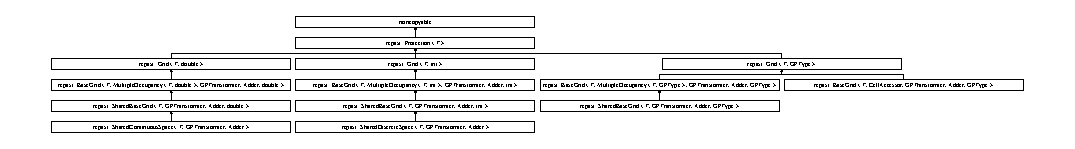
\includegraphics[height=1.552680cm]{classrepast_1_1_projection}
\end{center}
\end{figure}
\subsection*{Public Types}
\begin{DoxyCompactItemize}
\item 
enum {\bfseries R\-A\-D\-I\-U\-S} \{ {\bfseries P\-R\-I\-M\-A\-R\-Y}, 
{\bfseries S\-E\-C\-O\-N\-D\-A\-R\-Y}
 \}
\end{DoxyCompactItemize}
\subsection*{Public Member Functions}
\begin{DoxyCompactItemize}
\item 
\hyperlink{classrepast_1_1_projection_a2c5c9f33cf57c5e7a00402eab2080051}{Projection} (std\-::string \hyperlink{classrepast_1_1_projection_ab60a0ab4f584685780307d7431b61800}{name})
\begin{DoxyCompactList}\small\item\em Creates a projection with specified name. \end{DoxyCompactList}\item 
\hypertarget{classrepast_1_1_projection_ab60a0ab4f584685780307d7431b61800}{const std\-::string \hyperlink{classrepast_1_1_projection_ab60a0ab4f584685780307d7431b61800}{name} () const }\label{classrepast_1_1_projection_ab60a0ab4f584685780307d7431b61800}

\begin{DoxyCompactList}\small\item\em Gets the name of this projection. \end{DoxyCompactList}\item 
void \hyperlink{classrepast_1_1_projection_a340bcbf86f1e29489b9ca1a4aa5e9298}{add\-Filter\-Val} (int type)
\begin{DoxyCompactList}\small\item\em Adds an entry to the list of agent types that can be added to this projection. \end{DoxyCompactList}\item 
void \hyperlink{classrepast_1_1_projection_ab4587f793b1c250de22af16fedf7f89d}{remove\-Filter\-Val} (int type)
\begin{DoxyCompactList}\small\item\em Removes an entry from the list of agent types that can be added to this projection. \end{DoxyCompactList}\item 
\hypertarget{classrepast_1_1_projection_a35eae2c3351ef0de242a2ebeac8719df}{void \hyperlink{classrepast_1_1_projection_a35eae2c3351ef0de242a2ebeac8719df}{clear\-Filter} ()}\label{classrepast_1_1_projection_a35eae2c3351ef0de242a2ebeac8719df}

\begin{DoxyCompactList}\small\item\em Clears the list of agent types that can be added to this projection; the result is that the filter is empty, and any agent can be added. \end{DoxyCompactList}\item 
bool \hyperlink{classrepast_1_1_projection_a4075a777a46f27e978d376c90e74a409}{agent\-Can\-Be\-Added} (boost\-::shared\-\_\-ptr$<$ T $>$ agent)
\begin{DoxyCompactList}\small\item\em Returns true if the agent can be added to the projection, which will be the case if the filter list is empty or if the agent's type is in the filter list. \end{DoxyCompactList}\item 
virtual bool \hyperlink{classrepast_1_1_projection_a1da1dcc47517e3e25be129067b21601f}{keeps\-Agents\-On\-Sync\-Proj} ()=0
\begin{DoxyCompactList}\small\item\em Should return true if the \hyperlink{classrepast_1_1_projection}{Projection} implemented can 'keep' some (non-\/local) agents during a projection information synchronization operation. \end{DoxyCompactList}\item 
virtual bool \hyperlink{classrepast_1_1_projection_a686c52a83dd917e50b04f81dc7321ad7}{sends\-Secondary\-Agents\-On\-Status\-Exchange} ()=0
\begin{DoxyCompactList}\small\item\em Should return true if the \hyperlink{classrepast_1_1_projection}{Projection} implemented will send secondary agents during a status exchange. \end{DoxyCompactList}\item 
virtual void \hyperlink{classrepast_1_1_projection_afdc13fccb129094bfd67b3446873933d}{get\-Info\-Exchange\-Partners} (std\-::set$<$ int $>$ \&ps\-To\-Send\-To, std\-::set$<$ int $>$ \&ps\-To\-Receive\-From)=0
\begin{DoxyCompactList}\small\item\em Gets the set of processes with which this \hyperlink{classrepast_1_1_projection}{Projection} exchanges projection info. \end{DoxyCompactList}\item 
virtual void \hyperlink{classrepast_1_1_projection_ad2d104bb6119d0911053d450932855d5}{get\-Agent\-Status\-Exchange\-Partners} (std\-::set$<$ int $>$ \&ps\-To\-Send\-To, std\-::set$<$ int $>$ \&ps\-To\-Receive\-From)=0
\begin{DoxyCompactList}\small\item\em Gets the set of processes with which this \hyperlink{classrepast_1_1_projection}{Projection} exchanges agent status info-\/ that is, the set of processes from which agents can move to this one or to which they can move when moving from this one. \end{DoxyCompactList}\item 
virtual void \hyperlink{classrepast_1_1_projection_ad13ded8db8e364aa43efde5b35da9a65}{get\-Required\-Agents} (std\-::set$<$ \hyperlink{classrepast_1_1_agent_id}{Agent\-Id} $>$ \&agents\-To\-Test, std\-::set$<$ \hyperlink{classrepast_1_1_agent_id}{Agent\-Id} $>$ \&agents\-Required, R\-A\-D\-I\-U\-S radius=P\-R\-I\-M\-A\-R\-Y)=0
\begin{DoxyCompactList}\small\item\em Given a set of agents to test, gets the subset that must be kept in order to fulfill the projection's 'contract' to the specified radius. \end{DoxyCompactList}\item 
virtual void \hyperlink{classrepast_1_1_projection_ae1877809facd80a5e25d95e3dc5c35f4}{get\-Agents\-To\-Push} (std\-::set$<$ \hyperlink{classrepast_1_1_agent_id}{Agent\-Id} $>$ \&agents\-To\-Test, std\-::map$<$ int, std\-::set$<$ \hyperlink{classrepast_1_1_agent_id}{Agent\-Id} $>$ $>$ \&agents\-To\-Push)=0
\begin{DoxyCompactList}\small\item\em Given a set of agents, gets the agents that this projection implementation must 'push' to other processes. \end{DoxyCompactList}\item 
\hypertarget{classrepast_1_1_projection_ae66e268656f0baee2a7656d5eda6f4b9}{virtual void \hyperlink{classrepast_1_1_projection_ae66e268656f0baee2a7656d5eda6f4b9}{get\-Projection\-Info} (std\-::vector$<$ \hyperlink{classrepast_1_1_agent_id}{Agent\-Id} $>$ \&agents, std\-::vector$<$ \hyperlink{classrepast_1_1_projection_info_packet}{Projection\-Info\-Packet} $\ast$ $>$ \&packets, bool secondary\-Info=false, std\-::set$<$ \hyperlink{classrepast_1_1_agent_id}{Agent\-Id} $>$ $\ast$secondary\-Ids=0, int dest\-Proc=-\/1)}\label{classrepast_1_1_projection_ae66e268656f0baee2a7656d5eda6f4b9}

\begin{DoxyCompactList}\small\item\em Convenience wrapper that gets all of the projection information for the agents specified (calls implementation in child class that gets only the information for one agent). \end{DoxyCompactList}\item 
\hypertarget{classrepast_1_1_projection_ae89c14a3463d292ba1cd829204fbee71}{void \hyperlink{classrepast_1_1_projection_ae89c14a3463d292ba1cd829204fbee71}{update\-Projection\-Info} (std\-::vector$<$ \hyperlink{classrepast_1_1_projection_info_packet}{Projection\-Info\-Packet} $\ast$ $>$ \&pips, \hyperlink{classrepast_1_1_context}{Context}$<$ T $>$ $\ast$context)}\label{classrepast_1_1_projection_ae89c14a3463d292ba1cd829204fbee71}

\begin{DoxyCompactList}\small\item\em Updates the projection information for the agents in this projection according to the information contained in the vector of information packets passed. \end{DoxyCompactList}\item 
\hypertarget{classrepast_1_1_projection_a543d26d3a44b7f83ee363044ca6f4884}{virtual void {\bfseries clean\-Projection\-Info} (std\-::set$<$ \hyperlink{classrepast_1_1_agent_id}{Agent\-Id} $>$ \&agents\-To\-Keep)=0}\label{classrepast_1_1_projection_a543d26d3a44b7f83ee363044ca6f4884}

\item 
\hypertarget{classrepast_1_1_projection_afd5cda203753da3d565d7839f92589e8}{virtual void {\bfseries balance} ()}\label{classrepast_1_1_projection_afd5cda203753da3d565d7839f92589e8}

\end{DoxyCompactItemize}
\subsection*{Protected Member Functions}
\begin{DoxyCompactItemize}
\item 
\hypertarget{classrepast_1_1_projection_ac232dfc16ee5ccdb04d694abf79ce9a3}{virtual bool {\bfseries add\-Agent} (boost\-::shared\-\_\-ptr$<$ T $>$ agent)=0}\label{classrepast_1_1_projection_ac232dfc16ee5ccdb04d694abf79ce9a3}

\item 
\hypertarget{classrepast_1_1_projection_a804afdbcd384a23f7bf2c7a53209f272}{virtual void {\bfseries remove\-Agent} (T $\ast$agent)=0}\label{classrepast_1_1_projection_a804afdbcd384a23f7bf2c7a53209f272}

\item 
\hypertarget{classrepast_1_1_projection_af1e3b8e72e84bb73b6260b45cb2d20e5}{virtual \hyperlink{classrepast_1_1_projection_info_packet}{Projection\-Info\-Packet} $\ast$ {\bfseries get\-Projection\-Info} (\hyperlink{classrepast_1_1_agent_id}{Agent\-Id} id, bool secondary\-Info=false, std\-::set$<$ \hyperlink{classrepast_1_1_agent_id}{Agent\-Id} $>$ $\ast$secondary\-Ids=0, int dest\-Proc=-\/1)=0}\label{classrepast_1_1_projection_af1e3b8e72e84bb73b6260b45cb2d20e5}

\item 
\hypertarget{classrepast_1_1_projection_a20dfbb08e40a0425cbf56cb8864f27c4}{virtual void {\bfseries update\-Projection\-Info} (\hyperlink{classrepast_1_1_projection_info_packet}{Projection\-Info\-Packet} $\ast$pip, \hyperlink{classrepast_1_1_context}{Context}$<$ T $>$ $\ast$context)=0}\label{classrepast_1_1_projection_a20dfbb08e40a0425cbf56cb8864f27c4}

\end{DoxyCompactItemize}
\subsection*{Protected Attributes}
\begin{DoxyCompactItemize}
\item 
\hypertarget{classrepast_1_1_projection_a374d61a05feb62c25e2046170fbd2be4}{std\-::string {\bfseries name\-\_\-}}\label{classrepast_1_1_projection_a374d61a05feb62c25e2046170fbd2be4}

\item 
\hypertarget{classrepast_1_1_projection_ade2db74e98e56396c2a129a7aefeb19e}{std\-::set$<$ int $>$ {\bfseries filter}}\label{classrepast_1_1_projection_ade2db74e98e56396c2a129a7aefeb19e}

\end{DoxyCompactItemize}
\subsection*{Friends}
\begin{DoxyCompactItemize}
\item 
\hypertarget{classrepast_1_1_projection_ab1a0dad4095ba9621060e4c197f8fdfe}{class {\bfseries Context$<$ T $>$}}\label{classrepast_1_1_projection_ab1a0dad4095ba9621060e4c197f8fdfe}

\end{DoxyCompactItemize}


\subsection{Detailed Description}
\subsubsection*{template$<$typename T$>$class repast\-::\-Projection$<$ T $>$}

Abstract base class for all Projections. 

\subsection{Constructor \& Destructor Documentation}
\hypertarget{classrepast_1_1_projection_a2c5c9f33cf57c5e7a00402eab2080051}{\index{repast\-::\-Projection@{repast\-::\-Projection}!Projection@{Projection}}
\index{Projection@{Projection}!repast::Projection@{repast\-::\-Projection}}
\subsubsection[{Projection}]{\setlength{\rightskip}{0pt plus 5cm}template$<$typename T$>$ {\bf repast\-::\-Projection}$<$ T $>$\-::{\bf Projection} (
\begin{DoxyParamCaption}
\item[{std\-::string}]{name}
\end{DoxyParamCaption}
)\hspace{0.3cm}{\ttfamily [inline]}}}\label{classrepast_1_1_projection_a2c5c9f33cf57c5e7a00402eab2080051}


Creates a projection with specified name. 


\begin{DoxyParams}{Parameters}
{\em name} & the name of the projection. This must be unique across projections \\
\hline
\end{DoxyParams}


\subsection{Member Function Documentation}
\hypertarget{classrepast_1_1_projection_a340bcbf86f1e29489b9ca1a4aa5e9298}{\index{repast\-::\-Projection@{repast\-::\-Projection}!add\-Filter\-Val@{add\-Filter\-Val}}
\index{add\-Filter\-Val@{add\-Filter\-Val}!repast::Projection@{repast\-::\-Projection}}
\subsubsection[{add\-Filter\-Val}]{\setlength{\rightskip}{0pt plus 5cm}template$<$typename T$>$ void {\bf repast\-::\-Projection}$<$ T $>$\-::add\-Filter\-Val (
\begin{DoxyParamCaption}
\item[{int}]{type}
\end{DoxyParamCaption}
)\hspace{0.3cm}{\ttfamily [inline]}}}\label{classrepast_1_1_projection_a340bcbf86f1e29489b9ca1a4aa5e9298}


Adds an entry to the list of agent types that can be added to this projection. 

Note\-: no indication if type is already listed


\begin{DoxyParams}{Parameters}
{\em type} & type to be added \\
\hline
\end{DoxyParams}
\hypertarget{classrepast_1_1_projection_a4075a777a46f27e978d376c90e74a409}{\index{repast\-::\-Projection@{repast\-::\-Projection}!agent\-Can\-Be\-Added@{agent\-Can\-Be\-Added}}
\index{agent\-Can\-Be\-Added@{agent\-Can\-Be\-Added}!repast::Projection@{repast\-::\-Projection}}
\subsubsection[{agent\-Can\-Be\-Added}]{\setlength{\rightskip}{0pt plus 5cm}template$<$typename T$>$ bool {\bf repast\-::\-Projection}$<$ T $>$\-::agent\-Can\-Be\-Added (
\begin{DoxyParamCaption}
\item[{boost\-::shared\-\_\-ptr$<$ T $>$}]{agent}
\end{DoxyParamCaption}
)\hspace{0.3cm}{\ttfamily [inline]}}}\label{classrepast_1_1_projection_a4075a777a46f27e978d376c90e74a409}


Returns true if the agent can be added to the projection, which will be the case if the filter list is empty or if the agent's type is in the filter list. 


\begin{DoxyParams}{Parameters}
{\em agent} & pointer to the agent to be tested \\
\hline
\end{DoxyParams}
\hypertarget{classrepast_1_1_projection_ad2d104bb6119d0911053d450932855d5}{\index{repast\-::\-Projection@{repast\-::\-Projection}!get\-Agent\-Status\-Exchange\-Partners@{get\-Agent\-Status\-Exchange\-Partners}}
\index{get\-Agent\-Status\-Exchange\-Partners@{get\-Agent\-Status\-Exchange\-Partners}!repast::Projection@{repast\-::\-Projection}}
\subsubsection[{get\-Agent\-Status\-Exchange\-Partners}]{\setlength{\rightskip}{0pt plus 5cm}template$<$typename T$>$ virtual void {\bf repast\-::\-Projection}$<$ T $>$\-::get\-Agent\-Status\-Exchange\-Partners (
\begin{DoxyParamCaption}
\item[{std\-::set$<$ int $>$ \&}]{ps\-To\-Send\-To, }
\item[{std\-::set$<$ int $>$ \&}]{ps\-To\-Receive\-From}
\end{DoxyParamCaption}
)\hspace{0.3cm}{\ttfamily [pure virtual]}}}\label{classrepast_1_1_projection_ad2d104bb6119d0911053d450932855d5}


Gets the set of processes with which this \hyperlink{classrepast_1_1_projection}{Projection} exchanges agent status info-\/ that is, the set of processes from which agents can move to this one or to which they can move when moving from this one. 

In the most general case this will be all other processors. However, simulations where agents move in spaces will usually exchange agents only with a small subset of 'neighbor' processes, which is knowable in advance and constant. To accommodate the general case, the algorithm for exchanging information must poll all other processes to see which are sending to this one; if this is known in advance, this additional (expensive) step can be skipped. 

Implemented in \hyperlink{classrepast_1_1_shared_base_grid_a0388d98240eb59548058d3c45da702d7}{repast\-::\-Shared\-Base\-Grid$<$ T, G\-P\-Transformer, Adder, G\-P\-Type $>$}, \hyperlink{classrepast_1_1_shared_base_grid_a0388d98240eb59548058d3c45da702d7}{repast\-::\-Shared\-Base\-Grid$<$ T, G\-P\-Transformer, Adder, int $>$}, \hyperlink{classrepast_1_1_shared_base_grid_a0388d98240eb59548058d3c45da702d7}{repast\-::\-Shared\-Base\-Grid$<$ T, G\-P\-Transformer, Adder, double $>$}, \hyperlink{classrepast_1_1_graph_a3e9a52d6d45473260e2771fe426c8a15}{repast\-::\-Graph$<$ V, E, Ec, Ec\-M $>$}, \hyperlink{classrepast_1_1_grid_a748354698308fe0d0c0fe33a657109d1}{repast\-::\-Grid$<$ T, G\-P\-Type $>$}, \hyperlink{classrepast_1_1_grid_a748354698308fe0d0c0fe33a657109d1}{repast\-::\-Grid$<$ T, double $>$}, and \hyperlink{classrepast_1_1_grid_a748354698308fe0d0c0fe33a657109d1}{repast\-::\-Grid$<$ T, int $>$}.

\hypertarget{classrepast_1_1_projection_ae1877809facd80a5e25d95e3dc5c35f4}{\index{repast\-::\-Projection@{repast\-::\-Projection}!get\-Agents\-To\-Push@{get\-Agents\-To\-Push}}
\index{get\-Agents\-To\-Push@{get\-Agents\-To\-Push}!repast::Projection@{repast\-::\-Projection}}
\subsubsection[{get\-Agents\-To\-Push}]{\setlength{\rightskip}{0pt plus 5cm}template$<$typename T$>$ virtual void {\bf repast\-::\-Projection}$<$ T $>$\-::get\-Agents\-To\-Push (
\begin{DoxyParamCaption}
\item[{std\-::set$<$ {\bf Agent\-Id} $>$ \&}]{agents\-To\-Test, }
\item[{std\-::map$<$ int, std\-::set$<$ {\bf Agent\-Id} $>$ $>$ \&}]{agents\-To\-Push}
\end{DoxyParamCaption}
)\hspace{0.3cm}{\ttfamily [pure virtual]}}}\label{classrepast_1_1_projection_ae1877809facd80a5e25d95e3dc5c35f4}


Given a set of agents, gets the agents that this projection implementation must 'push' to other processes. 

Generally spaces must push agents that are in 'buffer zones' and graphs must push local agents that are vertices to master edges where the other vertex is non-\/ local. The results are returned per-\/process in the agents\-To\-Push map. 

Implemented in \hyperlink{classrepast_1_1_shared_base_grid_ab1486e7698288efc1218653d4e5e1e15}{repast\-::\-Shared\-Base\-Grid$<$ T, G\-P\-Transformer, Adder, G\-P\-Type $>$}, \hyperlink{classrepast_1_1_shared_base_grid_ab1486e7698288efc1218653d4e5e1e15}{repast\-::\-Shared\-Base\-Grid$<$ T, G\-P\-Transformer, Adder, int $>$}, \hyperlink{classrepast_1_1_shared_base_grid_ab1486e7698288efc1218653d4e5e1e15}{repast\-::\-Shared\-Base\-Grid$<$ T, G\-P\-Transformer, Adder, double $>$}, \hyperlink{classrepast_1_1_base_grid_a8f718ade5af8285f71151eea824ce3cd}{repast\-::\-Base\-Grid$<$ T, Cell\-Accessor, G\-P\-Transformer, Adder, G\-P\-Type $>$}, \hyperlink{classrepast_1_1_base_grid_a8f718ade5af8285f71151eea824ce3cd}{repast\-::\-Base\-Grid$<$ T, Multiple\-Occupancy$<$ T, double $>$, G\-P\-Transformer, Adder, double $>$}, \hyperlink{classrepast_1_1_base_grid_a8f718ade5af8285f71151eea824ce3cd}{repast\-::\-Base\-Grid$<$ T, Multiple\-Occupancy$<$ T, G\-P\-Type $>$, G\-P\-Transformer, Adder, G\-P\-Type $>$}, \hyperlink{classrepast_1_1_base_grid_a8f718ade5af8285f71151eea824ce3cd}{repast\-::\-Base\-Grid$<$ T, Multiple\-Occupancy$<$ T, int $>$, G\-P\-Transformer, Adder, int $>$}, \hyperlink{classrepast_1_1_graph_a011c1f0f065e5b8238c6783966c380eb}{repast\-::\-Graph$<$ V, E, Ec, Ec\-M $>$}, \hyperlink{classrepast_1_1_grid_aa83b294fc8765e2f8ee44d8238855460}{repast\-::\-Grid$<$ T, G\-P\-Type $>$}, \hyperlink{classrepast_1_1_grid_aa83b294fc8765e2f8ee44d8238855460}{repast\-::\-Grid$<$ T, double $>$}, \hyperlink{classrepast_1_1_grid_aa83b294fc8765e2f8ee44d8238855460}{repast\-::\-Grid$<$ T, int $>$}, and \hyperlink{classrepast_1_1_shared_discrete_space_a1f690e82e6b7ea6a279db020e12b4d21}{repast\-::\-Shared\-Discrete\-Space$<$ T, G\-P\-Transformer, Adder $>$}.

\hypertarget{classrepast_1_1_projection_afdc13fccb129094bfd67b3446873933d}{\index{repast\-::\-Projection@{repast\-::\-Projection}!get\-Info\-Exchange\-Partners@{get\-Info\-Exchange\-Partners}}
\index{get\-Info\-Exchange\-Partners@{get\-Info\-Exchange\-Partners}!repast::Projection@{repast\-::\-Projection}}
\subsubsection[{get\-Info\-Exchange\-Partners}]{\setlength{\rightskip}{0pt plus 5cm}template$<$typename T$>$ virtual void {\bf repast\-::\-Projection}$<$ T $>$\-::get\-Info\-Exchange\-Partners (
\begin{DoxyParamCaption}
\item[{std\-::set$<$ int $>$ \&}]{ps\-To\-Send\-To, }
\item[{std\-::set$<$ int $>$ \&}]{ps\-To\-Receive\-From}
\end{DoxyParamCaption}
)\hspace{0.3cm}{\ttfamily [pure virtual]}}}\label{classrepast_1_1_projection_afdc13fccb129094bfd67b3446873933d}


Gets the set of processes with which this \hyperlink{classrepast_1_1_projection}{Projection} exchanges projection info. 

In the most general case this will be all other processors; this is the case for graphs, where agent connections can be arbitrary. However, spaces usually exchange information only with a small subset of 'neighbor' processes, which is knowable in advance and constant. To accommodate the general case, the algorithm for exchanging information must poll all other processes to see which are sending to this one; if this is known in advance, this additional (expensive) step can be skipped. 

Implemented in \hyperlink{classrepast_1_1_shared_base_grid_af4323686714c4f6216125db5609c3184}{repast\-::\-Shared\-Base\-Grid$<$ T, G\-P\-Transformer, Adder, G\-P\-Type $>$}, \hyperlink{classrepast_1_1_shared_base_grid_af4323686714c4f6216125db5609c3184}{repast\-::\-Shared\-Base\-Grid$<$ T, G\-P\-Transformer, Adder, int $>$}, \hyperlink{classrepast_1_1_shared_base_grid_af4323686714c4f6216125db5609c3184}{repast\-::\-Shared\-Base\-Grid$<$ T, G\-P\-Transformer, Adder, double $>$}, \hyperlink{classrepast_1_1_graph_ab4200382f280c05f020611428507a134}{repast\-::\-Graph$<$ V, E, Ec, Ec\-M $>$}, \hyperlink{classrepast_1_1_grid_a57b4449e602392119eb4db3e0011de05}{repast\-::\-Grid$<$ T, G\-P\-Type $>$}, \hyperlink{classrepast_1_1_grid_a57b4449e602392119eb4db3e0011de05}{repast\-::\-Grid$<$ T, double $>$}, and \hyperlink{classrepast_1_1_grid_a57b4449e602392119eb4db3e0011de05}{repast\-::\-Grid$<$ T, int $>$}.

\hypertarget{classrepast_1_1_projection_ad13ded8db8e364aa43efde5b35da9a65}{\index{repast\-::\-Projection@{repast\-::\-Projection}!get\-Required\-Agents@{get\-Required\-Agents}}
\index{get\-Required\-Agents@{get\-Required\-Agents}!repast::Projection@{repast\-::\-Projection}}
\subsubsection[{get\-Required\-Agents}]{\setlength{\rightskip}{0pt plus 5cm}template$<$typename T$>$ virtual void {\bf repast\-::\-Projection}$<$ T $>$\-::get\-Required\-Agents (
\begin{DoxyParamCaption}
\item[{std\-::set$<$ {\bf Agent\-Id} $>$ \&}]{agents\-To\-Test, }
\item[{std\-::set$<$ {\bf Agent\-Id} $>$ \&}]{agents\-Required, }
\item[{R\-A\-D\-I\-U\-S}]{radius = {\ttfamily PRIMARY}}
\end{DoxyParamCaption}
)\hspace{0.3cm}{\ttfamily [pure virtual]}}}\label{classrepast_1_1_projection_ad13ded8db8e364aa43efde5b35da9a65}


Given a set of agents to test, gets the subset that must be kept in order to fulfill the projection's 'contract' to the specified radius. 

Generally spaces do not require any agents, but graphs do-\/ generally the non-\/local ends to master copies of edges. 

Implemented in \hyperlink{classrepast_1_1_grid_ab1ff08ad641de4f74eab53e30ad14eb6}{repast\-::\-Grid$<$ T, G\-P\-Type $>$}, \hyperlink{classrepast_1_1_grid_ab1ff08ad641de4f74eab53e30ad14eb6}{repast\-::\-Grid$<$ T, double $>$}, and \hyperlink{classrepast_1_1_grid_ab1ff08ad641de4f74eab53e30ad14eb6}{repast\-::\-Grid$<$ T, int $>$}.

\hypertarget{classrepast_1_1_projection_a1da1dcc47517e3e25be129067b21601f}{\index{repast\-::\-Projection@{repast\-::\-Projection}!keeps\-Agents\-On\-Sync\-Proj@{keeps\-Agents\-On\-Sync\-Proj}}
\index{keeps\-Agents\-On\-Sync\-Proj@{keeps\-Agents\-On\-Sync\-Proj}!repast::Projection@{repast\-::\-Projection}}
\subsubsection[{keeps\-Agents\-On\-Sync\-Proj}]{\setlength{\rightskip}{0pt plus 5cm}template$<$typename T$>$ virtual bool {\bf repast\-::\-Projection}$<$ T $>$\-::keeps\-Agents\-On\-Sync\-Proj (
\begin{DoxyParamCaption}
{}
\end{DoxyParamCaption}
)\hspace{0.3cm}{\ttfamily [pure virtual]}}}\label{classrepast_1_1_projection_a1da1dcc47517e3e25be129067b21601f}


Should return true if the \hyperlink{classrepast_1_1_projection}{Projection} implemented can 'keep' some (non-\/local) agents during a projection information synchronization operation. 

Generally spaces will allow all non-\/local agents to be deleted, but graphs keep the non-\/local agents that participate in Master edges.

It is possible to override these. A graph projection can be created that does not permit non-\/local agents to be 'kept'. This would be an extremely unusual use case, but it is possible.

Note that these are used for optimization. If no projection in a given context keeps any agents, several steps in the synchronization algorithm can be omitted. Of course, omitting these steps when a projection actually retains agents can caused undefined problems.

\begin{DoxyReturn}{Returns}
true if this projection will keep non-\/local agents during a projection information synchronziation event, false if it will not. 
\end{DoxyReturn}


Implemented in \hyperlink{classrepast_1_1_graph_aedaa8e44eb04056df2acabbeba373201}{repast\-::\-Graph$<$ V, E, Ec, Ec\-M $>$}, \hyperlink{classrepast_1_1_grid_aa46a5e7692430604bb3b04bbb9e2ff50}{repast\-::\-Grid$<$ T, G\-P\-Type $>$}, \hyperlink{classrepast_1_1_grid_aa46a5e7692430604bb3b04bbb9e2ff50}{repast\-::\-Grid$<$ T, double $>$}, and \hyperlink{classrepast_1_1_grid_aa46a5e7692430604bb3b04bbb9e2ff50}{repast\-::\-Grid$<$ T, int $>$}.

\hypertarget{classrepast_1_1_projection_ab4587f793b1c250de22af16fedf7f89d}{\index{repast\-::\-Projection@{repast\-::\-Projection}!remove\-Filter\-Val@{remove\-Filter\-Val}}
\index{remove\-Filter\-Val@{remove\-Filter\-Val}!repast::Projection@{repast\-::\-Projection}}
\subsubsection[{remove\-Filter\-Val}]{\setlength{\rightskip}{0pt plus 5cm}template$<$typename T$>$ void {\bf repast\-::\-Projection}$<$ T $>$\-::remove\-Filter\-Val (
\begin{DoxyParamCaption}
\item[{int}]{type}
\end{DoxyParamCaption}
)\hspace{0.3cm}{\ttfamily [inline]}}}\label{classrepast_1_1_projection_ab4587f793b1c250de22af16fedf7f89d}


Removes an entry from the list of agent types that can be added to this projection. 

Note\-: no indication if type is not listed


\begin{DoxyParams}{Parameters}
{\em type} & entry to be removed \\
\hline
\end{DoxyParams}
\hypertarget{classrepast_1_1_projection_a686c52a83dd917e50b04f81dc7321ad7}{\index{repast\-::\-Projection@{repast\-::\-Projection}!sends\-Secondary\-Agents\-On\-Status\-Exchange@{sends\-Secondary\-Agents\-On\-Status\-Exchange}}
\index{sends\-Secondary\-Agents\-On\-Status\-Exchange@{sends\-Secondary\-Agents\-On\-Status\-Exchange}!repast::Projection@{repast\-::\-Projection}}
\subsubsection[{sends\-Secondary\-Agents\-On\-Status\-Exchange}]{\setlength{\rightskip}{0pt plus 5cm}template$<$typename T$>$ virtual bool {\bf repast\-::\-Projection}$<$ T $>$\-::sends\-Secondary\-Agents\-On\-Status\-Exchange (
\begin{DoxyParamCaption}
{}
\end{DoxyParamCaption}
)\hspace{0.3cm}{\ttfamily [pure virtual]}}}\label{classrepast_1_1_projection_a686c52a83dd917e50b04f81dc7321ad7}


Should return true if the \hyperlink{classrepast_1_1_projection}{Projection} implemented will send secondary agents during a status exchange. 

Generally spaces do not and graphs do.

If no secondary agents will be sent, portions of the algorithm can be omitted for optimization.

\begin{DoxyReturn}{Returns}
true if the \hyperlink{classrepast_1_1_projection}{Projection} returns secondary agents, false if not 
\end{DoxyReturn}


Implemented in \hyperlink{classrepast_1_1_graph_a80cd467aae6d5e2c381bbe9cade6cbba}{repast\-::\-Graph$<$ V, E, Ec, Ec\-M $>$}, \hyperlink{classrepast_1_1_grid_ae3b7e2de573a9212a58a527a9ab519b8}{repast\-::\-Grid$<$ T, G\-P\-Type $>$}, \hyperlink{classrepast_1_1_grid_ae3b7e2de573a9212a58a527a9ab519b8}{repast\-::\-Grid$<$ T, double $>$}, and \hyperlink{classrepast_1_1_grid_ae3b7e2de573a9212a58a527a9ab519b8}{repast\-::\-Grid$<$ T, int $>$}.



The documentation for this class was generated from the following file\-:\begin{DoxyCompactItemize}
\item 
repast\-\_\-hpc/Projection.\-h\end{DoxyCompactItemize}

\hypertarget{classrepast_1_1_projection_info_packet}{\section{repast\-:\-:Projection\-Info\-Packet Class Reference}
\label{classrepast_1_1_projection_info_packet}\index{repast\-::\-Projection\-Info\-Packet@{repast\-::\-Projection\-Info\-Packet}}
}


Serializable packet that can contain projection information regardless of the type of projection (network or spatial).  




{\ttfamily \#include $<$Projection.\-h$>$}

Inheritance diagram for repast\-:\-:Projection\-Info\-Packet\-:\begin{figure}[H]
\begin{center}
\leavevmode
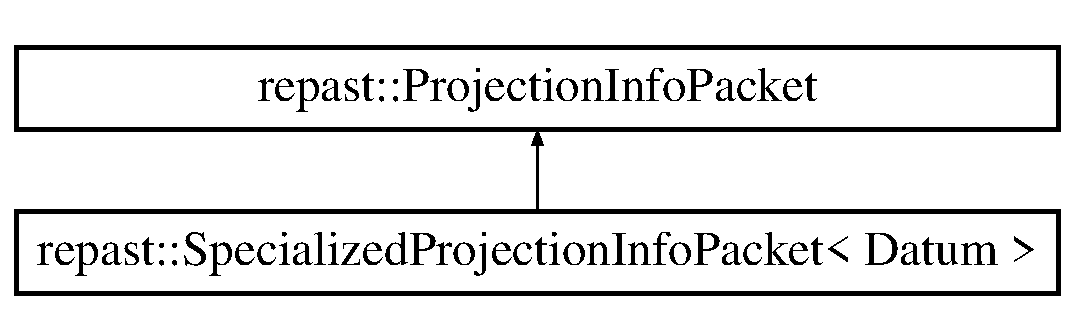
\includegraphics[height=2.000000cm]{classrepast_1_1_projection_info_packet}
\end{center}
\end{figure}
\subsection*{Public Member Functions}
\begin{DoxyCompactItemize}
\item 
\hypertarget{classrepast_1_1_projection_info_packet_a35712ffa6671be2c1932ed8fb58fb45d}{{\bfseries Projection\-Info\-Packet} (\hyperlink{classrepast_1_1_agent_id}{Agent\-Id} agent\-Id)}\label{classrepast_1_1_projection_info_packet_a35712ffa6671be2c1932ed8fb58fb45d}

\item 
\hypertarget{classrepast_1_1_projection_info_packet_a431829029f6f7108b89fc6dde27c4209}{{\footnotesize template$<$class Archive $>$ }\\void {\bfseries serialize} (Archive \&ar, const unsigned int version)}\label{classrepast_1_1_projection_info_packet_a431829029f6f7108b89fc6dde27c4209}

\item 
\hypertarget{classrepast_1_1_projection_info_packet_afbe080d5a5527b588465f07bfd061198}{virtual bool {\bfseries is\-Empty} ()}\label{classrepast_1_1_projection_info_packet_afbe080d5a5527b588465f07bfd061198}

\end{DoxyCompactItemize}
\subsection*{Public Attributes}
\begin{DoxyCompactItemize}
\item 
\hypertarget{classrepast_1_1_projection_info_packet_ae68c1d9e0a767a560546729f59a22307}{\hyperlink{classrepast_1_1_agent_id}{Agent\-Id} {\bfseries id}}\label{classrepast_1_1_projection_info_packet_ae68c1d9e0a767a560546729f59a22307}

\end{DoxyCompactItemize}
\subsection*{Friends}
\begin{DoxyCompactItemize}
\item 
\hypertarget{classrepast_1_1_projection_info_packet_ac98d07dd8f7b70e16ccb9a01abf56b9c}{class {\bfseries boost\-::serialization\-::access}}\label{classrepast_1_1_projection_info_packet_ac98d07dd8f7b70e16ccb9a01abf56b9c}

\end{DoxyCompactItemize}


\subsection{Detailed Description}
Serializable packet that can contain projection information regardless of the type of projection (network or spatial). 

The documentation for this class was generated from the following file\-:\begin{DoxyCompactItemize}
\item 
repast\-\_\-hpc/Projection.\-h\end{DoxyCompactItemize}

\hypertarget{classrepast_1_1_properties}{\section{repast\-:\-:Properties Class Reference}
\label{classrepast_1_1_properties}\index{repast\-::\-Properties@{repast\-::\-Properties}}
}


Map type object that contains key, value(string) properties.  




{\ttfamily \#include $<$Properties.\-h$>$}

\subsection*{Public Types}
\begin{DoxyCompactItemize}
\item 
\hypertarget{classrepast_1_1_properties_a033e3e16f3cfb8579fa09973ea3a53da}{typedef \\*
boost\-::transform\-\_\-iterator\\*
$<$ \hyperlink{structrepast_1_1_key_getter}{Key\-Getter}, std\-::map\\*
$<$ std\-::string, std\-::string $>$\\*
\-::const\-\_\-iterator $>$ {\bfseries key\-\_\-iterator}}\label{classrepast_1_1_properties_a033e3e16f3cfb8579fa09973ea3a53da}

\end{DoxyCompactItemize}
\subsection*{Public Member Functions}
\begin{DoxyCompactItemize}
\item 
\hypertarget{classrepast_1_1_properties_ab34048edde5f078749499e54ae33b092}{\hyperlink{classrepast_1_1_properties_ab34048edde5f078749499e54ae33b092}{Properties} ()}\label{classrepast_1_1_properties_ab34048edde5f078749499e54ae33b092}

\begin{DoxyCompactList}\small\item\em Creates an empty \hyperlink{classrepast_1_1_properties}{Properties}. \end{DoxyCompactList}\item 
\hyperlink{classrepast_1_1_properties_a23c9d9635eb8cf61b877692abf4d94b8}{Properties} (const std\-::string \&file, boost\-::mpi\-::communicator $\ast$comm=0, int max\-Prop\-File\-Size=M\-A\-X\-\_\-\-P\-R\-O\-P\-\_\-\-F\-I\-L\-E\-\_\-\-S\-I\-Z\-E)
\begin{DoxyCompactList}\small\item\em Creates a new \hyperlink{classrepast_1_1_properties}{Properties} using the properties defined in the specified file. \end{DoxyCompactList}\item 
\hyperlink{classrepast_1_1_properties_a15f789bec63f21941cd4d88a77c327c3}{Properties} (const std\-::string \&file, int argc, char $\ast$$\ast$argv, boost\-::mpi\-::communicator $\ast$comm=0, int max\-Prop\-File\-Size=M\-A\-X\-\_\-\-P\-R\-O\-P\-\_\-\-F\-I\-L\-E\-\_\-\-S\-I\-Z\-E)
\begin{DoxyCompactList}\small\item\em Creates a new \hyperlink{classrepast_1_1_properties}{Properties} using the properties defined in the specified file and any properties specified in Key=Val format in the argument array. \end{DoxyCompactList}\item 
\hyperlink{classrepast_1_1_properties_ab4edc85145fddc5d6dbd3dbf4d074ef7}{Properties} (int argc, char $\ast$$\ast$argv)
\begin{DoxyCompactList}\small\item\em Creates a new \hyperlink{classrepast_1_1_properties}{Properties} using the properties specified in Key=Val format in the argument. \end{DoxyCompactList}\item 
void \hyperlink{classrepast_1_1_properties_a9008647e3045dbd18356d43c9f343fe0}{put\-Property} (const std\-::string \&key, std\-::string value)
\begin{DoxyCompactList}\small\item\em Puts a property into this \hyperlink{classrepast_1_1_properties}{Properties} with the specified key and value. \end{DoxyCompactList}\item 
void \hyperlink{classrepast_1_1_properties_ae11bdd22268c15934237acc3cdfa1e91}{put\-Property} (const std\-::string \&key, long double value)
\begin{DoxyCompactList}\small\item\em Puts a property into this \hyperlink{classrepast_1_1_properties}{Properties} with the specified key and value. \end{DoxyCompactList}\item 
std\-::string \hyperlink{classrepast_1_1_properties_a10845b8c51a4f23b9fe8e4bb3b2402e7}{get\-Property} (const std\-::string \&key) const 
\begin{DoxyCompactList}\small\item\em Gets the property with the specified key. \end{DoxyCompactList}\item 
bool \hyperlink{classrepast_1_1_properties_a00995681d4adf3abcd8910a6a1bb72ee}{contains} (const std\-::string \&key) const 
\begin{DoxyCompactList}\small\item\em Gets whether or not this \hyperlink{classrepast_1_1_properties}{Properties} contains the specified key. \end{DoxyCompactList}\item 
key\-\_\-iterator \hyperlink{classrepast_1_1_properties_aa3ec0c363bc6ccdc033aa6dc7cc29f70}{keys\-\_\-begin} () const 
\begin{DoxyCompactList}\small\item\em Gets the start of an iterator over this \hyperlink{classrepast_1_1_properties}{Properties}' keys. \end{DoxyCompactList}\item 
key\-\_\-iterator \hyperlink{classrepast_1_1_properties_a0b2a76982e541649e237ed8c59c86de6}{keys\-\_\-end} () const 
\begin{DoxyCompactList}\small\item\em Gets the end of an iterator over this \hyperlink{classrepast_1_1_properties}{Properties}' keys. \end{DoxyCompactList}\item 
void \hyperlink{classrepast_1_1_properties_a85536ec978c9077c3447bcc4a9422608}{read\-File} (const std\-::string \&file, boost\-::mpi\-::communicator $\ast$comm=0, int max\-Prop\-File\-Size=M\-A\-X\-\_\-\-P\-R\-O\-P\-\_\-\-F\-I\-L\-E\-\_\-\-S\-I\-Z\-E)
\begin{DoxyCompactList}\small\item\em Adds any properties defined in the specified file. \end{DoxyCompactList}\item 
void \hyperlink{classrepast_1_1_properties_a8fb65d329a032b1c21c77e60d9a54a85}{process\-Command\-Line\-Arguments} (int argc, char $\ast$$\ast$argv)
\begin{DoxyCompactList}\small\item\em Processes a char$\ast$$\ast$ array of the given size; any component that has an equals sign is entered as a property value, overriding any previous entry read from the properies file. \end{DoxyCompactList}\item 
int \hyperlink{classrepast_1_1_properties_afa2c5157a67086937da071b2ecbc6f86}{size} () const 
\begin{DoxyCompactList}\small\item\em Gets the number of properties in this \hyperlink{classrepast_1_1_properties}{Properties}. \end{DoxyCompactList}\item 
void \hyperlink{classrepast_1_1_properties_ae0ad23f9e0ac85943969847fb4372f9d}{log} (std\-::string log\-Name, std\-::vector$<$ std\-::string $>$ $\ast$keys\-To\-Write=0)
\begin{DoxyCompactList}\small\item\em Writes the contents of the properties file to the specified repast log (at 'I\-N\-F\-O' log level) \end{DoxyCompactList}\item 
void \hyperlink{classrepast_1_1_properties_a82b48502a6403ad5c929ae30d0470c9d}{write\-To\-S\-V\-File} (std\-::string file\-Name, std\-::string separator=\char`\"{},\char`\"{})
\begin{DoxyCompactList}\small\item\em Writes the contents of the properties file to the specified separated-\/value file. \end{DoxyCompactList}\item 
void \hyperlink{classrepast_1_1_properties_ad7f85154fb7f657e5bfaee197fc391c4}{write\-To\-S\-V\-File} (std\-::string file\-Name, std\-::vector$<$ std\-::string $>$ \&keys\-To\-Write, std\-::string separator=\char`\"{},\char`\"{})
\begin{DoxyCompactList}\small\item\em Writes the contents of the properties file to the specified separated-\/value file. \end{DoxyCompactList}\end{DoxyCompactItemize}


\subsection{Detailed Description}
Map type object that contains key, value(string) properties. 

A \hyperlink{classrepast_1_1_properties}{Properties} instance can be constructed from a file. Each line is a property with the key and value separated by =. For example,

some.\-property = 3\par
 another.\-property = hello 

\subsection{Constructor \& Destructor Documentation}
\hypertarget{classrepast_1_1_properties_a23c9d9635eb8cf61b877692abf4d94b8}{\index{repast\-::\-Properties@{repast\-::\-Properties}!Properties@{Properties}}
\index{Properties@{Properties}!repast::Properties@{repast\-::\-Properties}}
\subsubsection[{Properties}]{\setlength{\rightskip}{0pt plus 5cm}repast\-::\-Properties\-::\-Properties (
\begin{DoxyParamCaption}
\item[{const std\-::string \&}]{file, }
\item[{boost\-::mpi\-::communicator $\ast$}]{comm = {\ttfamily 0}, }
\item[{int}]{max\-Prop\-File\-Size = {\ttfamily MAX\-\_\-PROP\-\_\-FILE\-\_\-SIZE}}
\end{DoxyParamCaption}
)}}\label{classrepast_1_1_properties_a23c9d9635eb8cf61b877692abf4d94b8}


Creates a new \hyperlink{classrepast_1_1_properties}{Properties} using the properties defined in the specified file. 

Each line is a property with the key and value separated by =. For example,

some.\-property = 3\par
 another.\-property = hello


\begin{DoxyParams}{Parameters}
{\em file} & the properties file path \\
\hline
{\em comm} & pointer to a communicator; if null (the default), all processes read the properties file separately. If a communicator is provided, rank 0 reads the file and broadcasts it to all other ranks. \\
\hline
{\em max\-Prop\-File\-Size} & optional parameter; if the properties file is larger than the default M\-A\-X\-\_\-\-P\-R\-O\-P\-\_\-\-F\-I\-L\-E\-\_\-\-S\-I\-Z\-E, the new size can be passed here. \\
\hline
\end{DoxyParams}
\hypertarget{classrepast_1_1_properties_a15f789bec63f21941cd4d88a77c327c3}{\index{repast\-::\-Properties@{repast\-::\-Properties}!Properties@{Properties}}
\index{Properties@{Properties}!repast::Properties@{repast\-::\-Properties}}
\subsubsection[{Properties}]{\setlength{\rightskip}{0pt plus 5cm}repast\-::\-Properties\-::\-Properties (
\begin{DoxyParamCaption}
\item[{const std\-::string \&}]{file, }
\item[{int}]{argc, }
\item[{char $\ast$$\ast$}]{argv, }
\item[{boost\-::mpi\-::communicator $\ast$}]{comm = {\ttfamily 0}, }
\item[{int}]{max\-Prop\-File\-Size = {\ttfamily MAX\-\_\-PROP\-\_\-FILE\-\_\-SIZE}}
\end{DoxyParamCaption}
)}}\label{classrepast_1_1_properties_a15f789bec63f21941cd4d88a77c327c3}


Creates a new \hyperlink{classrepast_1_1_properties}{Properties} using the properties defined in the specified file and any properties specified in Key=Val format in the argument array. 

\hyperlink{classrepast_1_1_properties}{Properties} in the argument array will supersede any in the properties file.

Each line in the properties file is a property with the key and value separated by =. For example,

some.\-property = 3\par
 another.\-property = hello


\begin{DoxyParams}{Parameters}
{\em file} & the properties file path \\
\hline
{\em argc} & count of the elements in the argv array \\
\hline
{\em array} & of char$\ast$ that may include Key=Value pairs. Elements with no '=' are ignored. \\
\hline
{\em comm} & pointer to a communicator; if null (the default), all processes read the properties file separately. If a communicator is provided, rank 0 reads the file and broadcasts it to all other ranks. \\
\hline
{\em max\-Prop\-File\-Size} & optional parameter; if the properties file is larger than the default M\-A\-X\-\_\-\-P\-R\-O\-P\-\_\-\-F\-I\-L\-E\-\_\-\-S\-I\-Z\-E, the new size can be passed here. \\
\hline
\end{DoxyParams}
\hypertarget{classrepast_1_1_properties_ab4edc85145fddc5d6dbd3dbf4d074ef7}{\index{repast\-::\-Properties@{repast\-::\-Properties}!Properties@{Properties}}
\index{Properties@{Properties}!repast::Properties@{repast\-::\-Properties}}
\subsubsection[{Properties}]{\setlength{\rightskip}{0pt plus 5cm}repast\-::\-Properties\-::\-Properties (
\begin{DoxyParamCaption}
\item[{int}]{argc, }
\item[{char $\ast$$\ast$}]{argv}
\end{DoxyParamCaption}
)}}\label{classrepast_1_1_properties_ab4edc85145fddc5d6dbd3dbf4d074ef7}


Creates a new \hyperlink{classrepast_1_1_properties}{Properties} using the properties specified in Key=Val format in the argument. 


\begin{DoxyParams}{Parameters}
{\em argc} & count of the elements in the argv array \\
\hline
{\em array} & of char$\ast$ that may include Key=Value pairs. Elements with no '=' are ignored. \\
\hline
\end{DoxyParams}


\subsection{Member Function Documentation}
\hypertarget{classrepast_1_1_properties_a00995681d4adf3abcd8910a6a1bb72ee}{\index{repast\-::\-Properties@{repast\-::\-Properties}!contains@{contains}}
\index{contains@{contains}!repast::Properties@{repast\-::\-Properties}}
\subsubsection[{contains}]{\setlength{\rightskip}{0pt plus 5cm}bool repast\-::\-Properties\-::contains (
\begin{DoxyParamCaption}
\item[{const std\-::string \&}]{key}
\end{DoxyParamCaption}
) const}}\label{classrepast_1_1_properties_a00995681d4adf3abcd8910a6a1bb72ee}


Gets whether or not this \hyperlink{classrepast_1_1_properties}{Properties} contains the specified key. 


\begin{DoxyParams}{Parameters}
{\em key} & the property key \\
\hline
\end{DoxyParams}
\hypertarget{classrepast_1_1_properties_a10845b8c51a4f23b9fe8e4bb3b2402e7}{\index{repast\-::\-Properties@{repast\-::\-Properties}!get\-Property@{get\-Property}}
\index{get\-Property@{get\-Property}!repast::Properties@{repast\-::\-Properties}}
\subsubsection[{get\-Property}]{\setlength{\rightskip}{0pt plus 5cm}string repast\-::\-Properties\-::get\-Property (
\begin{DoxyParamCaption}
\item[{const std\-::string \&}]{key}
\end{DoxyParamCaption}
) const}}\label{classrepast_1_1_properties_a10845b8c51a4f23b9fe8e4bb3b2402e7}


Gets the property with the specified key. 


\begin{DoxyParams}{Parameters}
{\em key} & the property key\\
\hline
\end{DoxyParams}
\begin{DoxyReturn}{Returns}
the value for that key, or an empty string if the property is not found. 
\end{DoxyReturn}
\hypertarget{classrepast_1_1_properties_aa3ec0c363bc6ccdc033aa6dc7cc29f70}{\index{repast\-::\-Properties@{repast\-::\-Properties}!keys\-\_\-begin@{keys\-\_\-begin}}
\index{keys\-\_\-begin@{keys\-\_\-begin}!repast::Properties@{repast\-::\-Properties}}
\subsubsection[{keys\-\_\-begin}]{\setlength{\rightskip}{0pt plus 5cm}key\-\_\-iterator repast\-::\-Properties\-::keys\-\_\-begin (
\begin{DoxyParamCaption}
{}
\end{DoxyParamCaption}
) const\hspace{0.3cm}{\ttfamily [inline]}}}\label{classrepast_1_1_properties_aa3ec0c363bc6ccdc033aa6dc7cc29f70}


Gets the start of an iterator over this \hyperlink{classrepast_1_1_properties}{Properties}' keys. 

\begin{DoxyReturn}{Returns}
the start of an iterator over this \hyperlink{classrepast_1_1_properties}{Properties}' keys. 
\end{DoxyReturn}
\hypertarget{classrepast_1_1_properties_a0b2a76982e541649e237ed8c59c86de6}{\index{repast\-::\-Properties@{repast\-::\-Properties}!keys\-\_\-end@{keys\-\_\-end}}
\index{keys\-\_\-end@{keys\-\_\-end}!repast::Properties@{repast\-::\-Properties}}
\subsubsection[{keys\-\_\-end}]{\setlength{\rightskip}{0pt plus 5cm}key\-\_\-iterator repast\-::\-Properties\-::keys\-\_\-end (
\begin{DoxyParamCaption}
{}
\end{DoxyParamCaption}
) const\hspace{0.3cm}{\ttfamily [inline]}}}\label{classrepast_1_1_properties_a0b2a76982e541649e237ed8c59c86de6}


Gets the end of an iterator over this \hyperlink{classrepast_1_1_properties}{Properties}' keys. 

\begin{DoxyReturn}{Returns}
the end of an iterator over this \hyperlink{classrepast_1_1_properties}{Properties}' keys. 
\end{DoxyReturn}
\hypertarget{classrepast_1_1_properties_ae0ad23f9e0ac85943969847fb4372f9d}{\index{repast\-::\-Properties@{repast\-::\-Properties}!log@{log}}
\index{log@{log}!repast::Properties@{repast\-::\-Properties}}
\subsubsection[{log}]{\setlength{\rightskip}{0pt plus 5cm}void repast\-::\-Properties\-::log (
\begin{DoxyParamCaption}
\item[{std\-::string}]{log\-Name, }
\item[{std\-::vector$<$ std\-::string $>$ $\ast$}]{keys\-To\-Write = {\ttfamily 0}}
\end{DoxyParamCaption}
)\hspace{0.3cm}{\ttfamily [inline]}}}\label{classrepast_1_1_properties_ae0ad23f9e0ac85943969847fb4372f9d}


Writes the contents of the properties file to the specified repast log (at 'I\-N\-F\-O' log level) 


\begin{DoxyParams}{Parameters}
{\em log\-Name} & name of the log to use \\
\hline
{\em keys\-To\-Write} & optional; if included, writes only the keys included in the vector and their values, in the order they appear in the vector. Will write blank values for any key name in the vector that is not in the properties file. If not included, all properties and their values are written, in map order. \\
\hline
\end{DoxyParams}
\hypertarget{classrepast_1_1_properties_a8fb65d329a032b1c21c77e60d9a54a85}{\index{repast\-::\-Properties@{repast\-::\-Properties}!process\-Command\-Line\-Arguments@{process\-Command\-Line\-Arguments}}
\index{process\-Command\-Line\-Arguments@{process\-Command\-Line\-Arguments}!repast::Properties@{repast\-::\-Properties}}
\subsubsection[{process\-Command\-Line\-Arguments}]{\setlength{\rightskip}{0pt plus 5cm}void repast\-::\-Properties\-::process\-Command\-Line\-Arguments (
\begin{DoxyParamCaption}
\item[{int}]{argc, }
\item[{char $\ast$$\ast$}]{argv}
\end{DoxyParamCaption}
)}}\label{classrepast_1_1_properties_a8fb65d329a032b1c21c77e60d9a54a85}


Processes a char$\ast$$\ast$ array of the given size; any component that has an equals sign is entered as a property value, overriding any previous entry read from the properies file. 


\begin{DoxyParams}{Parameters}
{\em argc} & the number of entries in the array \\
\hline
{\em argv} & the array of char values to be mapped \\
\hline
\end{DoxyParams}
\hypertarget{classrepast_1_1_properties_a9008647e3045dbd18356d43c9f343fe0}{\index{repast\-::\-Properties@{repast\-::\-Properties}!put\-Property@{put\-Property}}
\index{put\-Property@{put\-Property}!repast::Properties@{repast\-::\-Properties}}
\subsubsection[{put\-Property}]{\setlength{\rightskip}{0pt plus 5cm}void repast\-::\-Properties\-::put\-Property (
\begin{DoxyParamCaption}
\item[{const std\-::string \&}]{key, }
\item[{std\-::string}]{value}
\end{DoxyParamCaption}
)}}\label{classrepast_1_1_properties_a9008647e3045dbd18356d43c9f343fe0}


Puts a property into this \hyperlink{classrepast_1_1_properties}{Properties} with the specified key and value. 


\begin{DoxyParams}{Parameters}
{\em key} & the property key \\
\hline
{\em value} & the property value \\
\hline
\end{DoxyParams}
\hypertarget{classrepast_1_1_properties_ae11bdd22268c15934237acc3cdfa1e91}{\index{repast\-::\-Properties@{repast\-::\-Properties}!put\-Property@{put\-Property}}
\index{put\-Property@{put\-Property}!repast::Properties@{repast\-::\-Properties}}
\subsubsection[{put\-Property}]{\setlength{\rightskip}{0pt plus 5cm}void repast\-::\-Properties\-::put\-Property (
\begin{DoxyParamCaption}
\item[{const std\-::string \&}]{key, }
\item[{long double}]{value}
\end{DoxyParamCaption}
)}}\label{classrepast_1_1_properties_ae11bdd22268c15934237acc3cdfa1e91}


Puts a property into this \hyperlink{classrepast_1_1_properties}{Properties} with the specified key and value. 

Note that even though the second argument can be passed as a numeric value, it is stored as a string


\begin{DoxyParams}{Parameters}
{\em key} & the property key \\
\hline
{\em value} & the property value \\
\hline
\end{DoxyParams}
\hypertarget{classrepast_1_1_properties_a85536ec978c9077c3447bcc4a9422608}{\index{repast\-::\-Properties@{repast\-::\-Properties}!read\-File@{read\-File}}
\index{read\-File@{read\-File}!repast::Properties@{repast\-::\-Properties}}
\subsubsection[{read\-File}]{\setlength{\rightskip}{0pt plus 5cm}void repast\-::\-Properties\-::read\-File (
\begin{DoxyParamCaption}
\item[{const std\-::string \&}]{file, }
\item[{boost\-::mpi\-::communicator $\ast$}]{comm = {\ttfamily 0}, }
\item[{int}]{max\-Prop\-File\-Size = {\ttfamily MAX\-\_\-PROP\-\_\-FILE\-\_\-SIZE}}
\end{DoxyParamCaption}
)}}\label{classrepast_1_1_properties_a85536ec978c9077c3447bcc4a9422608}


Adds any properties defined in the specified file. 

Each line is a property with the key and value separated by =. For example,

some.\-property = 3\par
 another.\-property = hello


\begin{DoxyParams}{Parameters}
{\em file} & the properties file path \\
\hline
{\em comm} & pointer to a communicator; if null (the default), all processes read the properties file separately. If a communicator is provided, rank 0 reads the file and broadcasts it to all other ranks. \\
\hline
\end{DoxyParams}
\hypertarget{classrepast_1_1_properties_afa2c5157a67086937da071b2ecbc6f86}{\index{repast\-::\-Properties@{repast\-::\-Properties}!size@{size}}
\index{size@{size}!repast::Properties@{repast\-::\-Properties}}
\subsubsection[{size}]{\setlength{\rightskip}{0pt plus 5cm}int repast\-::\-Properties\-::size (
\begin{DoxyParamCaption}
{}
\end{DoxyParamCaption}
) const\hspace{0.3cm}{\ttfamily [inline]}}}\label{classrepast_1_1_properties_afa2c5157a67086937da071b2ecbc6f86}


Gets the number of properties in this \hyperlink{classrepast_1_1_properties}{Properties}. 

\begin{DoxyReturn}{Returns}
the number of properties in this \hyperlink{classrepast_1_1_properties}{Properties}. 
\end{DoxyReturn}
\hypertarget{classrepast_1_1_properties_a82b48502a6403ad5c929ae30d0470c9d}{\index{repast\-::\-Properties@{repast\-::\-Properties}!write\-To\-S\-V\-File@{write\-To\-S\-V\-File}}
\index{write\-To\-S\-V\-File@{write\-To\-S\-V\-File}!repast::Properties@{repast\-::\-Properties}}
\subsubsection[{write\-To\-S\-V\-File}]{\setlength{\rightskip}{0pt plus 5cm}void repast\-::\-Properties\-::write\-To\-S\-V\-File (
\begin{DoxyParamCaption}
\item[{std\-::string}]{file\-Name, }
\item[{std\-::string}]{separator = {\ttfamily \char`\"{},\char`\"{}}}
\end{DoxyParamCaption}
)}}\label{classrepast_1_1_properties_a82b48502a6403ad5c929ae30d0470c9d}


Writes the contents of the properties file to the specified separated-\/value file. 

If the file does not exist it is created and a header line is written with the key values.


\begin{DoxyParams}{Parameters}
{\em file\-Name} & name \\
\hline
\end{DoxyParams}
\hypertarget{classrepast_1_1_properties_ad7f85154fb7f657e5bfaee197fc391c4}{\index{repast\-::\-Properties@{repast\-::\-Properties}!write\-To\-S\-V\-File@{write\-To\-S\-V\-File}}
\index{write\-To\-S\-V\-File@{write\-To\-S\-V\-File}!repast::Properties@{repast\-::\-Properties}}
\subsubsection[{write\-To\-S\-V\-File}]{\setlength{\rightskip}{0pt plus 5cm}void repast\-::\-Properties\-::write\-To\-S\-V\-File (
\begin{DoxyParamCaption}
\item[{std\-::string}]{file\-Name, }
\item[{std\-::vector$<$ std\-::string $>$ \&}]{keys\-To\-Write, }
\item[{std\-::string}]{separator = {\ttfamily \char`\"{},\char`\"{}}}
\end{DoxyParamCaption}
)}}\label{classrepast_1_1_properties_ad7f85154fb7f657e5bfaee197fc391c4}


Writes the contents of the properties file to the specified separated-\/value file. 

If the file does not exist it is created and a header line is written with the key values.


\begin{DoxyParams}{Parameters}
{\em file\-Name} & name \\
\hline
\end{DoxyParams}


The documentation for this class was generated from the following files\-:\begin{DoxyCompactItemize}
\item 
repast\-\_\-hpc/Properties.\-h\item 
repast\-\_\-hpc/Properties.\-cpp\end{DoxyCompactItemize}

\hypertarget{classrepast_1_1_random}{\section{repast\-:\-:Random Class Reference}
\label{classrepast_1_1_random}\index{repast\-::\-Random@{repast\-::\-Random}}
}


Methods for working with random distributions, draws etc.  




{\ttfamily \#include $<$Random.\-h$>$}

\subsection*{Public Member Functions}
\begin{DoxyCompactItemize}
\item 
void \hyperlink{classrepast_1_1_random_af3e9c83a19e18347f05dbd0fe7044144}{put\-Generator} (const std\-::string \&id, \hyperlink{classrepast_1_1_number_generator}{Number\-Generator} $\ast$generator)
\begin{DoxyCompactList}\small\item\em Puts the named generator into this \hyperlink{classrepast_1_1_random}{Random}. \end{DoxyCompactList}\item 
\hyperlink{classrepast_1_1_number_generator}{Number\-Generator} $\ast$ \hyperlink{classrepast_1_1_random_ae74efa6b1d2a91054538378f6488b066}{get\-Generator} (const std\-::string \&id)
\begin{DoxyCompactList}\small\item\em Gets the named generator or 0 if the name is not found. \end{DoxyCompactList}\item 
boost\-::mt19937 \& \hyperlink{classrepast_1_1_random_ac3bcb79b02d9158f2d681a6887ec1f6f}{engine} ()
\begin{DoxyCompactList}\small\item\em Gets the random number engine from which the distributions are created. \end{DoxyCompactList}\item 
boost\-::uint32\-\_\-t \hyperlink{classrepast_1_1_random_abc9590ab2bbd9a61bc1af7c1f72bb604}{seed} ()
\begin{DoxyCompactList}\small\item\em Gets the current seed. \end{DoxyCompactList}\item 
double \hyperlink{classrepast_1_1_random_aac8516b6a9f9005013dafc82034ce2e3}{next\-Double} ()
\begin{DoxyCompactList}\small\item\em Gets the next double in the range \mbox{[}0, 1). \end{DoxyCompactList}\item 
\hyperlink{classrepast_1_1_default_number_generator}{Double\-Uniform\-Generator} \hyperlink{classrepast_1_1_random_a5017a5f8427219f9e0d487f4ae2b215d}{create\-Uni\-Double\-Generator} (double from, double to)
\begin{DoxyCompactList}\small\item\em Creates a generator that produces doubles in the range \mbox{[}from, to). \end{DoxyCompactList}\item 
\hyperlink{classrepast_1_1_default_number_generator}{Int\-Uniform\-Generator} \hyperlink{classrepast_1_1_random_a5263c2b66369177674e2d223d5ff7945}{create\-Uni\-Int\-Generator} (int from, int to)
\begin{DoxyCompactList}\small\item\em Creates a generator that produces ints in the range \mbox{[}from, to\mbox{]}. \end{DoxyCompactList}\item 
\hyperlink{classrepast_1_1_default_number_generator}{Triangle\-Generator} \hyperlink{classrepast_1_1_random_a405c6638702359ebc0038dc309a73a45}{create\-Triangle\-Generator} (double lower\-Bound, double most\-Likely, double upper\-Bound)
\begin{DoxyCompactList}\small\item\em Creates a triangle generator with the specified properties. \end{DoxyCompactList}\item 
\hyperlink{classrepast_1_1_default_number_generator}{Cauchy\-Generator} \hyperlink{classrepast_1_1_random_a59e3fefc2dc6406b25ad00c0250ca12e}{create\-Cauchy\-Generator} (double median, double sigma)
\begin{DoxyCompactList}\small\item\em pdf\-: p(x) = sigma/(pi$\ast$(sigma$\ast$$\ast$2 + (x-\/median)$\ast$$\ast$2)) \end{DoxyCompactList}\item 
\hyperlink{classrepast_1_1_default_number_generator}{Exponential\-Generator} \hyperlink{classrepast_1_1_random_a223f65315bcc4a07087116719b5fa251}{create\-Exponential\-Generator} (double lambda)
\begin{DoxyCompactList}\small\item\em pdf\-: p(x) = lambda $\ast$ exp(-\/lambda $\ast$ x) \end{DoxyCompactList}\item 
\hyperlink{classrepast_1_1_default_number_generator}{Normal\-Generator} \hyperlink{classrepast_1_1_random_a33226e423e66a9fcd3e3cdf3c9ce62ae}{create\-Normal\-Generator} (double mean, double sigma)
\begin{DoxyCompactList}\small\item\em Creates a normal generator. \end{DoxyCompactList}\item 
\hypertarget{classrepast_1_1_random_aff15cda637d1579444379195681aa5d4}{\hyperlink{classrepast_1_1_default_number_generator}{Log\-Normal\-Generator} \hyperlink{classrepast_1_1_random_aff15cda637d1579444379195681aa5d4}{create\-Log\-Normal\-Generator} (double mean, double sigma)}\label{classrepast_1_1_random_aff15cda637d1579444379195681aa5d4}

\begin{DoxyCompactList}\small\item\em Produces random numbers with p(x) = 1/(x $\ast$ normal\-\_\-sigma $\ast$ sqrt(2$\ast$pi)) $\ast$ exp( -\/(log(x)-\/normal\-\_\-mean)2 / (2$\ast$normal\-\_\-sigma2) ) for x $>$ 0, where normal\-\_\-mean = log(mean2/sqrt(sigma2 + mean2)) and normal\-\_\-sigma = sqrt(log(1 + sigma2/mean2)) \end{DoxyCompactList}\end{DoxyCompactItemize}
\subsection*{Static Public Member Functions}
\begin{DoxyCompactItemize}
\item 
static void \hyperlink{classrepast_1_1_random_aff5e636ed06991e91b149e880944022e}{initialize} (boost\-::uint32\-\_\-t \hyperlink{classrepast_1_1_random_abc9590ab2bbd9a61bc1af7c1f72bb604}{seed})
\begin{DoxyCompactList}\small\item\em Initialize the \hyperlink{classrepast_1_1_random}{Random} singleton with the specified seed. \end{DoxyCompactList}\item 
\hypertarget{classrepast_1_1_random_abd9ca1f149eda9adf01c48174caa6734}{static \hyperlink{classrepast_1_1_random}{Random} $\ast$ \hyperlink{classrepast_1_1_random_abd9ca1f149eda9adf01c48174caa6734}{instance} ()}\label{classrepast_1_1_random_abd9ca1f149eda9adf01c48174caa6734}

\begin{DoxyCompactList}\small\item\em Gets the singleton instance of this \hyperlink{classrepast_1_1_random}{Random}. \end{DoxyCompactList}\end{DoxyCompactItemize}
\subsection*{Protected Member Functions}
\begin{DoxyCompactItemize}
\item 
\hypertarget{classrepast_1_1_random_aa2f7a12fcf5b872549684405cb196139}{{\bfseries Random} (boost\-::uint32\-\_\-t \hyperlink{classrepast_1_1_random_abc9590ab2bbd9a61bc1af7c1f72bb604}{seed})}\label{classrepast_1_1_random_aa2f7a12fcf5b872549684405cb196139}

\end{DoxyCompactItemize}


\subsection{Detailed Description}
Methods for working with random distributions, draws etc. 

\subsection{Member Function Documentation}
\hypertarget{classrepast_1_1_random_a59e3fefc2dc6406b25ad00c0250ca12e}{\index{repast\-::\-Random@{repast\-::\-Random}!create\-Cauchy\-Generator@{create\-Cauchy\-Generator}}
\index{create\-Cauchy\-Generator@{create\-Cauchy\-Generator}!repast::Random@{repast\-::\-Random}}
\subsubsection[{create\-Cauchy\-Generator}]{\setlength{\rightskip}{0pt plus 5cm}{\bf Cauchy\-Generator} repast\-::\-Random\-::create\-Cauchy\-Generator (
\begin{DoxyParamCaption}
\item[{double}]{median, }
\item[{double}]{sigma}
\end{DoxyParamCaption}
)}}\label{classrepast_1_1_random_a59e3fefc2dc6406b25ad00c0250ca12e}


pdf\-: p(x) = sigma/(pi$\ast$(sigma$\ast$$\ast$2 + (x-\/median)$\ast$$\ast$2)) 


\begin{DoxyParams}{Parameters}
{\em median} & \\
\hline
{\em sigma} & \\
\hline
\end{DoxyParams}
\begin{DoxyReturn}{Returns}
a Cauchy generator. 
\end{DoxyReturn}
\hypertarget{classrepast_1_1_random_a223f65315bcc4a07087116719b5fa251}{\index{repast\-::\-Random@{repast\-::\-Random}!create\-Exponential\-Generator@{create\-Exponential\-Generator}}
\index{create\-Exponential\-Generator@{create\-Exponential\-Generator}!repast::Random@{repast\-::\-Random}}
\subsubsection[{create\-Exponential\-Generator}]{\setlength{\rightskip}{0pt plus 5cm}{\bf Exponential\-Generator} repast\-::\-Random\-::create\-Exponential\-Generator (
\begin{DoxyParamCaption}
\item[{double}]{lambda}
\end{DoxyParamCaption}
)}}\label{classrepast_1_1_random_a223f65315bcc4a07087116719b5fa251}


pdf\-: p(x) = lambda $\ast$ exp(-\/lambda $\ast$ x) 


\begin{DoxyParams}{Parameters}
{\em lambda} & must be $>$ 0\\
\hline
\end{DoxyParams}
\begin{DoxyReturn}{Returns}
an exponential generator. 
\end{DoxyReturn}
\hypertarget{classrepast_1_1_random_a33226e423e66a9fcd3e3cdf3c9ce62ae}{\index{repast\-::\-Random@{repast\-::\-Random}!create\-Normal\-Generator@{create\-Normal\-Generator}}
\index{create\-Normal\-Generator@{create\-Normal\-Generator}!repast::Random@{repast\-::\-Random}}
\subsubsection[{create\-Normal\-Generator}]{\setlength{\rightskip}{0pt plus 5cm}{\bf Normal\-Generator} repast\-::\-Random\-::create\-Normal\-Generator (
\begin{DoxyParamCaption}
\item[{double}]{mean, }
\item[{double}]{sigma}
\end{DoxyParamCaption}
)}}\label{classrepast_1_1_random_a33226e423e66a9fcd3e3cdf3c9ce62ae}


Creates a normal generator. 

pdf\-: p(x) = 1/sqrt(2$\ast$pi$\ast$sigma) $\ast$ exp(-\/ (x-\/mean)2 / (2$\ast$sigma2) ) \hypertarget{classrepast_1_1_random_a405c6638702359ebc0038dc309a73a45}{\index{repast\-::\-Random@{repast\-::\-Random}!create\-Triangle\-Generator@{create\-Triangle\-Generator}}
\index{create\-Triangle\-Generator@{create\-Triangle\-Generator}!repast::Random@{repast\-::\-Random}}
\subsubsection[{create\-Triangle\-Generator}]{\setlength{\rightskip}{0pt plus 5cm}{\bf Triangle\-Generator} repast\-::\-Random\-::create\-Triangle\-Generator (
\begin{DoxyParamCaption}
\item[{double}]{lower\-Bound, }
\item[{double}]{most\-Likely, }
\item[{double}]{upper\-Bound}
\end{DoxyParamCaption}
)}}\label{classrepast_1_1_random_a405c6638702359ebc0038dc309a73a45}


Creates a triangle generator with the specified properties. 

A Triangle\-Generator produces a floating point value x where lowerbound $<$= x $<$= upper\-Bound and most\-Likely is the most probable value for x.


\begin{DoxyParams}{Parameters}
{\em lower\-Bound} & the lower bound of the values produced by the generator \\
\hline
{\em most\-Likely} & the most likely value produced by the generator \\
\hline
{\em upper\-Bound} & the upper bound of the values produced by the generator\\
\hline
\end{DoxyParams}
\begin{DoxyReturn}{Returns}
a triangle generator. 
\end{DoxyReturn}
\hypertarget{classrepast_1_1_random_a5017a5f8427219f9e0d487f4ae2b215d}{\index{repast\-::\-Random@{repast\-::\-Random}!create\-Uni\-Double\-Generator@{create\-Uni\-Double\-Generator}}
\index{create\-Uni\-Double\-Generator@{create\-Uni\-Double\-Generator}!repast::Random@{repast\-::\-Random}}
\subsubsection[{create\-Uni\-Double\-Generator}]{\setlength{\rightskip}{0pt plus 5cm}{\bf Double\-Uniform\-Generator} repast\-::\-Random\-::create\-Uni\-Double\-Generator (
\begin{DoxyParamCaption}
\item[{double}]{from, }
\item[{double}]{to}
\end{DoxyParamCaption}
)}}\label{classrepast_1_1_random_a5017a5f8427219f9e0d487f4ae2b215d}


Creates a generator that produces doubles in the range \mbox{[}from, to). 

inclusive of from, exclusive of to.


\begin{DoxyParams}{Parameters}
{\em from} & the range start (inclusive) \\
\hline
{\em to} & the range end (exclusive)\\
\hline
\end{DoxyParams}
\begin{DoxyReturn}{Returns}
a generator that produces doubles in the range \mbox{[}from, to). 
\end{DoxyReturn}
\hypertarget{classrepast_1_1_random_a5263c2b66369177674e2d223d5ff7945}{\index{repast\-::\-Random@{repast\-::\-Random}!create\-Uni\-Int\-Generator@{create\-Uni\-Int\-Generator}}
\index{create\-Uni\-Int\-Generator@{create\-Uni\-Int\-Generator}!repast::Random@{repast\-::\-Random}}
\subsubsection[{create\-Uni\-Int\-Generator}]{\setlength{\rightskip}{0pt plus 5cm}{\bf Int\-Uniform\-Generator} repast\-::\-Random\-::create\-Uni\-Int\-Generator (
\begin{DoxyParamCaption}
\item[{int}]{from, }
\item[{int}]{to}
\end{DoxyParamCaption}
)}}\label{classrepast_1_1_random_a5263c2b66369177674e2d223d5ff7945}


Creates a generator that produces ints in the range \mbox{[}from, to\mbox{]}. 


\begin{DoxyParams}{Parameters}
{\em from} & the range start (inclusive) \\
\hline
{\em to} & the range end (inclusive)\\
\hline
\end{DoxyParams}
\begin{DoxyReturn}{Returns}
a generator that produces ints in the range \mbox{[}from, to\mbox{]}. 
\end{DoxyReturn}
\hypertarget{classrepast_1_1_random_ac3bcb79b02d9158f2d681a6887ec1f6f}{\index{repast\-::\-Random@{repast\-::\-Random}!engine@{engine}}
\index{engine@{engine}!repast::Random@{repast\-::\-Random}}
\subsubsection[{engine}]{\setlength{\rightskip}{0pt plus 5cm}boost\-::mt19937\& repast\-::\-Random\-::engine (
\begin{DoxyParamCaption}
{}
\end{DoxyParamCaption}
)\hspace{0.3cm}{\ttfamily [inline]}}}\label{classrepast_1_1_random_ac3bcb79b02d9158f2d681a6887ec1f6f}


Gets the random number engine from which the distributions are created. 

\begin{DoxyReturn}{Returns}
he random number engine from which the distributions are created. 
\end{DoxyReturn}
\hypertarget{classrepast_1_1_random_ae74efa6b1d2a91054538378f6488b066}{\index{repast\-::\-Random@{repast\-::\-Random}!get\-Generator@{get\-Generator}}
\index{get\-Generator@{get\-Generator}!repast::Random@{repast\-::\-Random}}
\subsubsection[{get\-Generator}]{\setlength{\rightskip}{0pt plus 5cm}{\bf Number\-Generator} $\ast$ repast\-::\-Random\-::get\-Generator (
\begin{DoxyParamCaption}
\item[{const std\-::string \&}]{id}
\end{DoxyParamCaption}
)}}\label{classrepast_1_1_random_ae74efa6b1d2a91054538378f6488b066}


Gets the named generator or 0 if the name is not found. 


\begin{DoxyParams}{Parameters}
{\em id} & the name of the generator to get \\
\hline
\end{DoxyParams}
\hypertarget{classrepast_1_1_random_aff5e636ed06991e91b149e880944022e}{\index{repast\-::\-Random@{repast\-::\-Random}!initialize@{initialize}}
\index{initialize@{initialize}!repast::Random@{repast\-::\-Random}}
\subsubsection[{initialize}]{\setlength{\rightskip}{0pt plus 5cm}void repast\-::\-Random\-::initialize (
\begin{DoxyParamCaption}
\item[{boost\-::uint32\-\_\-t}]{seed}
\end{DoxyParamCaption}
)\hspace{0.3cm}{\ttfamily [static]}}}\label{classrepast_1_1_random_aff5e636ed06991e91b149e880944022e}


Initialize the \hyperlink{classrepast_1_1_random}{Random} singleton with the specified seed. 


\begin{DoxyParams}{Parameters}
{\em the} & seed to initialize the random number generator with. \\
\hline
\end{DoxyParams}
\hypertarget{classrepast_1_1_random_aac8516b6a9f9005013dafc82034ce2e3}{\index{repast\-::\-Random@{repast\-::\-Random}!next\-Double@{next\-Double}}
\index{next\-Double@{next\-Double}!repast::Random@{repast\-::\-Random}}
\subsubsection[{next\-Double}]{\setlength{\rightskip}{0pt plus 5cm}double repast\-::\-Random\-::next\-Double (
\begin{DoxyParamCaption}
{}
\end{DoxyParamCaption}
)}}\label{classrepast_1_1_random_aac8516b6a9f9005013dafc82034ce2e3}


Gets the next double in the range \mbox{[}0, 1). 

\begin{DoxyReturn}{Returns}
the next double in the range \mbox{[}0, 1). 
\end{DoxyReturn}
\hypertarget{classrepast_1_1_random_af3e9c83a19e18347f05dbd0fe7044144}{\index{repast\-::\-Random@{repast\-::\-Random}!put\-Generator@{put\-Generator}}
\index{put\-Generator@{put\-Generator}!repast::Random@{repast\-::\-Random}}
\subsubsection[{put\-Generator}]{\setlength{\rightskip}{0pt plus 5cm}void repast\-::\-Random\-::put\-Generator (
\begin{DoxyParamCaption}
\item[{const std\-::string \&}]{id, }
\item[{{\bf Number\-Generator} $\ast$}]{generator}
\end{DoxyParamCaption}
)}}\label{classrepast_1_1_random_af3e9c83a19e18347f05dbd0fe7044144}


Puts the named generator into this \hyperlink{classrepast_1_1_random}{Random}. 

Added generators will be deleted by \hyperlink{classrepast_1_1_random}{Random} when it is destroyed.


\begin{DoxyParams}{Parameters}
{\em the} & id of the generator \\
\hline
{\em generator} & the generator to add \\
\hline
\end{DoxyParams}
\hypertarget{classrepast_1_1_random_abc9590ab2bbd9a61bc1af7c1f72bb604}{\index{repast\-::\-Random@{repast\-::\-Random}!seed@{seed}}
\index{seed@{seed}!repast::Random@{repast\-::\-Random}}
\subsubsection[{seed}]{\setlength{\rightskip}{0pt plus 5cm}boost\-::uint32\-\_\-t repast\-::\-Random\-::seed (
\begin{DoxyParamCaption}
{}
\end{DoxyParamCaption}
)\hspace{0.3cm}{\ttfamily [inline]}}}\label{classrepast_1_1_random_abc9590ab2bbd9a61bc1af7c1f72bb604}


Gets the current seed. 

\begin{DoxyReturn}{Returns}
the current seed. 
\end{DoxyReturn}


The documentation for this class was generated from the following files\-:\begin{DoxyCompactItemize}
\item 
repast\-\_\-hpc/Random.\-h\item 
repast\-\_\-hpc/Random.\-cpp\end{DoxyCompactItemize}

\hypertarget{classrepast_1_1_random_access}{\section{repast\-:\-:Random\-Access$<$ I $>$ Class Template Reference}
\label{classrepast_1_1_random_access}\index{repast\-::\-Random\-Access$<$ I $>$@{repast\-::\-Random\-Access$<$ I $>$}}
}


Given an iterator and a number of elements, creates a data structure that allows efficient access to those elements.  




{\ttfamily \#include $<$Random.\-h$>$}

\subsection*{Public Member Functions}
\begin{DoxyCompactItemize}
\item 
\hyperlink{classrepast_1_1_random_access_a44b227e4aabb796ca349fd01e533855b}{Random\-Access} (I beginning, int size)
\begin{DoxyCompactList}\small\item\em Constructs a \hyperlink{classrepast_1_1_random_access}{Random\-Access} instance for this iterator. \end{DoxyCompactList}\item 
I \hyperlink{classrepast_1_1_random_access_a8964a8f07e2efcc26ecf3df1a1ad59b9}{get} (int index)
\begin{DoxyCompactList}\small\item\em Gets the element at the specified index. \end{DoxyCompactList}\end{DoxyCompactItemize}


\subsection{Detailed Description}
\subsubsection*{template$<$typename I$>$class repast\-::\-Random\-Access$<$ I $>$}

Given an iterator and a number of elements, creates a data structure that allows efficient access to those elements. 

Is only valid as long as the iterator is valid.

The basic implementation creates a vector of ordered pairs linking an integer and an iterator pointing to an element in the original iteration set. To find the nth element, the algorithm searches backwards through the list of 'landmarks', finds the highest landmark lower than n, chooses the iterator associated with that landmark, and steps forward until n is reached, adding new landmarks if appropriate. So given landmarks\-:

0 -\/ pointer to element 0 100 -\/ pointer to element 100 200 -\/ pointer to element 200

if the request for element 438 is given, the algorithm will search backward and find landmark 200; it will then step forward, adding landmarks for 300 and 400, until element 438 is reached and returned.

Assuming that requests are evenly distributed, optimum interval for landmarks is the square root of the size of the list, and performance for the algorithm will be in log(size) time.

Note that other implementations are possible-\/ for example, checking if enough memory would allow a completely indexed list. A long-\/term possibility is allowing the user to specify (for example, specify that the algorithm with lowest memory cost be used even though memory is initially available, perhaps because other routines will be filling that memory while this object is in use). 

\subsection{Constructor \& Destructor Documentation}
\hypertarget{classrepast_1_1_random_access_a44b227e4aabb796ca349fd01e533855b}{\index{repast\-::\-Random\-Access@{repast\-::\-Random\-Access}!Random\-Access@{Random\-Access}}
\index{Random\-Access@{Random\-Access}!repast::RandomAccess@{repast\-::\-Random\-Access}}
\subsubsection[{Random\-Access}]{\setlength{\rightskip}{0pt plus 5cm}template$<$typename I $>$ {\bf repast\-::\-Random\-Access}$<$ I $>$\-::{\bf Random\-Access} (
\begin{DoxyParamCaption}
\item[{I}]{beginning, }
\item[{int}]{size}
\end{DoxyParamCaption}
)\hspace{0.3cm}{\ttfamily [inline]}}}\label{classrepast_1_1_random_access_a44b227e4aabb796ca349fd01e533855b}


Constructs a \hyperlink{classrepast_1_1_random_access}{Random\-Access} instance for this iterator. 


\begin{DoxyParams}{Parameters}
{\em beginning} & \\
\hline
{\em size} & \\
\hline
\end{DoxyParams}


\subsection{Member Function Documentation}
\hypertarget{classrepast_1_1_random_access_a8964a8f07e2efcc26ecf3df1a1ad59b9}{\index{repast\-::\-Random\-Access@{repast\-::\-Random\-Access}!get@{get}}
\index{get@{get}!repast::RandomAccess@{repast\-::\-Random\-Access}}
\subsubsection[{get}]{\setlength{\rightskip}{0pt plus 5cm}template$<$typename I $>$ I {\bf repast\-::\-Random\-Access}$<$ I $>$\-::get (
\begin{DoxyParamCaption}
\item[{int}]{index}
\end{DoxyParamCaption}
)\hspace{0.3cm}{\ttfamily [inline]}}}\label{classrepast_1_1_random_access_a8964a8f07e2efcc26ecf3df1a1ad59b9}


Gets the element at the specified index. 


\begin{DoxyParams}{Parameters}
{\em index} & \\
\hline
\end{DoxyParams}


The documentation for this class was generated from the following file\-:\begin{DoxyCompactItemize}
\item 
repast\-\_\-hpc/Random.\-h\end{DoxyCompactItemize}

\hypertarget{classrepast_1_1_reducible_data_source}{\section{repast\-:\-:Reducible\-Data\-Source$<$ Op, T $>$ Class Template Reference}
\label{classrepast_1_1_reducible_data_source}\index{repast\-::\-Reducible\-Data\-Source$<$ Op, T $>$@{repast\-::\-Reducible\-Data\-Source$<$ Op, T $>$}}
}


Source of data and a reduction operation.  




{\ttfamily \#include $<$Reducible\-Data\-Source.\-h$>$}

Inheritance diagram for repast\-:\-:Reducible\-Data\-Source$<$ Op, T $>$\-:\begin{figure}[H]
\begin{center}
\leavevmode
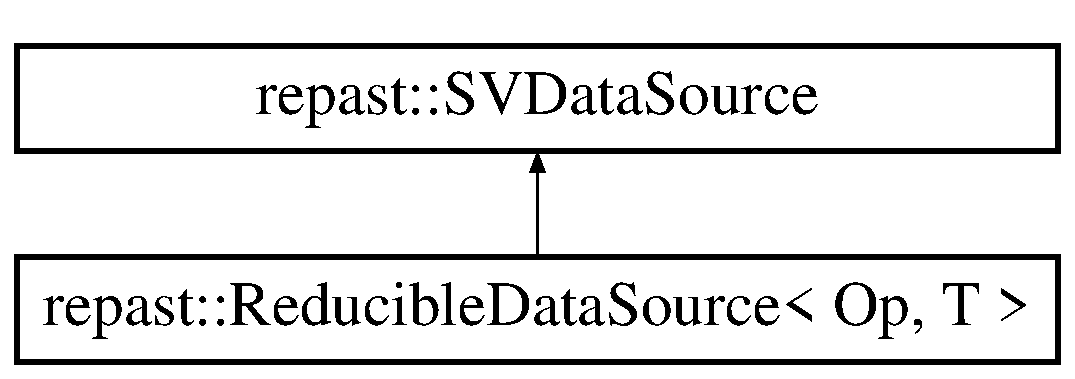
\includegraphics[height=2.000000cm]{classrepast_1_1_reducible_data_source}
\end{center}
\end{figure}
\subsection*{Public Member Functions}
\begin{DoxyCompactItemize}
\item 
\hypertarget{classrepast_1_1_reducible_data_source_a47e67b6bab27187c7a3ad62c7b97d7e5}{{\bfseries Reducible\-Data\-Source} (std\-::string name, \hyperlink{classrepast_1_1_t_data_source}{T\-Data\-Source}$<$ T $>$ $\ast$data\-Source, Op op)}\label{classrepast_1_1_reducible_data_source_a47e67b6bab27187c7a3ad62c7b97d7e5}

\item 
\hypertarget{classrepast_1_1_reducible_data_source_a349460403802a8c73d24ab03f2b3f87b}{virtual void {\bfseries record} ()}\label{classrepast_1_1_reducible_data_source_a349460403802a8c73d24ab03f2b3f87b}

\item 
\hypertarget{classrepast_1_1_reducible_data_source_a456dcb8f5ac22a6579ff31266dbb0846}{virtual void {\bfseries write} (\hyperlink{classrepast_1_1_variable}{Variable} $\ast$var)}\label{classrepast_1_1_reducible_data_source_a456dcb8f5ac22a6579ff31266dbb0846}

\item 
\hypertarget{classrepast_1_1_reducible_data_source_a5efa9f1e70161eaa6f5070551172d1ed}{virtual S\-V\-Data\-Source\-::\-Data\-Type {\bfseries type} () const }\label{classrepast_1_1_reducible_data_source_a5efa9f1e70161eaa6f5070551172d1ed}

\end{DoxyCompactItemize}
\subsection*{Protected Attributes}
\begin{DoxyCompactItemize}
\item 
\hypertarget{classrepast_1_1_reducible_data_source_a26e1f75855e72a423dd5cb362f992535}{Op {\bfseries \-\_\-op}}\label{classrepast_1_1_reducible_data_source_a26e1f75855e72a423dd5cb362f992535}

\item 
\hypertarget{classrepast_1_1_reducible_data_source_ad83152c79acdf6db218591c1984af1f2}{std\-::vector$<$ T $>$ {\bfseries data}}\label{classrepast_1_1_reducible_data_source_ad83152c79acdf6db218591c1984af1f2}

\item 
\hypertarget{classrepast_1_1_reducible_data_source_a09765379b1cfb5704ec642e51aebbd74}{\hyperlink{classrepast_1_1_t_data_source}{T\-Data\-Source}$<$ T $>$ $\ast$ {\bfseries \-\_\-data\-Source}}\label{classrepast_1_1_reducible_data_source_a09765379b1cfb5704ec642e51aebbd74}

\item 
\hypertarget{classrepast_1_1_reducible_data_source_a8511ef8c34d008f18e555f17c843596e}{int {\bfseries rank}}\label{classrepast_1_1_reducible_data_source_a8511ef8c34d008f18e555f17c843596e}

\end{DoxyCompactItemize}


\subsection{Detailed Description}
\subsubsection*{template$<$typename Op, typename T$>$class repast\-::\-Reducible\-Data\-Source$<$ Op, T $>$}

Source of data and a reduction operation. 

Used internally by a \hyperlink{classrepast_1_1_s_v_data_set}{S\-V\-Data\-Set} to store the data sources. their associated ops etc. 

The documentation for this class was generated from the following file\-:\begin{DoxyCompactItemize}
\item 
repast\-\_\-hpc/Reducible\-Data\-Source.\-h\end{DoxyCompactItemize}

\hypertarget{classrepast_1_1_repast_edge}{\section{repast\-:\-:Repast\-Edge$<$ V $>$ Class Template Reference}
\label{classrepast_1_1_repast_edge}\index{repast\-::\-Repast\-Edge$<$ V $>$@{repast\-::\-Repast\-Edge$<$ V $>$}}
}


Default graph / network edge implementation.  




{\ttfamily \#include $<$Edge.\-h$>$}

\subsection*{Public Types}
\begin{DoxyCompactItemize}
\item 
enum {\bfseries M\-A\-S\-T\-E\-R\-\_\-\-N\-O\-D\-E} \{ {\bfseries D\-E\-F\-A\-U\-L\-T}, 
{\bfseries S\-O\-U\-R\-C\-E}, 
{\bfseries T\-A\-R\-G\-E\-T}
 \}
\end{DoxyCompactItemize}
\subsection*{Public Member Functions}
\begin{DoxyCompactItemize}
\item 
\hyperlink{classrepast_1_1_repast_edge_ac0205e3ee8478344fba85730fcacae14}{Repast\-Edge} (V $\ast$\hyperlink{classrepast_1_1_repast_edge_a9b8886cb5295f847eccf9743a5f5b0a1}{source}, V $\ast$\hyperlink{classrepast_1_1_repast_edge_a971ec6e45b597d2068ac42125f1b4657}{target}, M\-A\-S\-T\-E\-R\-\_\-\-N\-O\-D\-E use\-Target\-As\-Master=D\-E\-F\-A\-U\-L\-T)
\begin{DoxyCompactList}\small\item\em Creates a \hyperlink{classrepast_1_1_repast_edge}{Repast\-Edge} with the specified source and target and a default weight of 1. \end{DoxyCompactList}\item 
\hyperlink{classrepast_1_1_repast_edge_a7aaad47c69b124500c6e75e631805825}{Repast\-Edge} (V $\ast$\hyperlink{classrepast_1_1_repast_edge_a9b8886cb5295f847eccf9743a5f5b0a1}{source}, V $\ast$\hyperlink{classrepast_1_1_repast_edge_a971ec6e45b597d2068ac42125f1b4657}{target}, double \hyperlink{classrepast_1_1_repast_edge_a6402b40ba110f9f531edf345399a8e74}{weight}, M\-A\-S\-T\-E\-R\-\_\-\-N\-O\-D\-E use\-Target\-As\-Master=D\-E\-F\-A\-U\-L\-T)
\begin{DoxyCompactList}\small\item\em Creates a \hyperlink{classrepast_1_1_repast_edge}{Repast\-Edge} with the specified source, target, and weight. \end{DoxyCompactList}\item 
\hyperlink{classrepast_1_1_repast_edge_a3dbb0517855e4e69ec46da6f956b879f}{Repast\-Edge} (boost\-::shared\-\_\-ptr$<$ V $>$ \hyperlink{classrepast_1_1_repast_edge_a9b8886cb5295f847eccf9743a5f5b0a1}{source}, boost\-::shared\-\_\-ptr$<$ V $>$ \hyperlink{classrepast_1_1_repast_edge_a971ec6e45b597d2068ac42125f1b4657}{target}, M\-A\-S\-T\-E\-R\-\_\-\-N\-O\-D\-E use\-Target\-As\-Master=D\-E\-F\-A\-U\-L\-T)
\begin{DoxyCompactList}\small\item\em Creates a \hyperlink{classrepast_1_1_repast_edge}{Repast\-Edge} with the specified source and target and a default weight of 1. \end{DoxyCompactList}\item 
\hyperlink{classrepast_1_1_repast_edge_ab0a726b1f69af0a1c3a22b9e53a3aead}{Repast\-Edge} (boost\-::shared\-\_\-ptr$<$ V $>$ \hyperlink{classrepast_1_1_repast_edge_a9b8886cb5295f847eccf9743a5f5b0a1}{source}, boost\-::shared\-\_\-ptr$<$ V $>$ \hyperlink{classrepast_1_1_repast_edge_a971ec6e45b597d2068ac42125f1b4657}{target}, double \hyperlink{classrepast_1_1_repast_edge_a6402b40ba110f9f531edf345399a8e74}{weight}, M\-A\-S\-T\-E\-R\-\_\-\-N\-O\-D\-E use\-Target\-As\-Master=D\-E\-F\-A\-U\-L\-T)
\begin{DoxyCompactList}\small\item\em Creates a \hyperlink{classrepast_1_1_repast_edge}{Repast\-Edge} with the specified source, target, and weight. \end{DoxyCompactList}\item 
\hypertarget{classrepast_1_1_repast_edge_aad7896812a552f85f70993c136b50f22}{\hyperlink{classrepast_1_1_repast_edge_aad7896812a552f85f70993c136b50f22}{Repast\-Edge} (const \hyperlink{classrepast_1_1_repast_edge}{Repast\-Edge} \&edge)}\label{classrepast_1_1_repast_edge_aad7896812a552f85f70993c136b50f22}

\begin{DoxyCompactList}\small\item\em Copy constructor that creates a \hyperlink{classrepast_1_1_repast_edge}{Repast\-Edge} from another \hyperlink{classrepast_1_1_repast_edge}{Repast\-Edge}. \end{DoxyCompactList}\item 
V $\ast$ \hyperlink{classrepast_1_1_repast_edge_a9b8886cb5295f847eccf9743a5f5b0a1}{source} () const 
\begin{DoxyCompactList}\small\item\em Gets the source of this \hyperlink{classrepast_1_1_repast_edge}{Repast\-Edge}. \end{DoxyCompactList}\item 
V $\ast$ \hyperlink{classrepast_1_1_repast_edge_a971ec6e45b597d2068ac42125f1b4657}{target} () const 
\begin{DoxyCompactList}\small\item\em Gets the target of this \hyperlink{classrepast_1_1_repast_edge}{Repast\-Edge}. \end{DoxyCompactList}\item 
\hypertarget{classrepast_1_1_repast_edge_a6b9889dbf6373654471c555c23dda130}{void {\bfseries target} (V $\ast$target)}\label{classrepast_1_1_repast_edge_a6b9889dbf6373654471c555c23dda130}

\item 
\hypertarget{classrepast_1_1_repast_edge_a1d4230ade56d772c452497a79d096adb}{void {\bfseries source} (V $\ast$source)}\label{classrepast_1_1_repast_edge_a1d4230ade56d772c452497a79d096adb}

\item 
double \hyperlink{classrepast_1_1_repast_edge_a6402b40ba110f9f531edf345399a8e74}{weight} () const 
\begin{DoxyCompactList}\small\item\em Gets the weight of this \hyperlink{classrepast_1_1_repast_edge}{Repast\-Edge}. \end{DoxyCompactList}\item 
\hypertarget{classrepast_1_1_repast_edge_aa620175d8226f8d19049e1f6a91560b6}{void {\bfseries weight} (double wt)}\label{classrepast_1_1_repast_edge_aa620175d8226f8d19049e1f6a91560b6}

\item 
\hypertarget{classrepast_1_1_repast_edge_a626a0ef621f1fe10f1e9856b6381e4a4}{bool {\bfseries uses\-Target\-As\-Master} ()}\label{classrepast_1_1_repast_edge_a626a0ef621f1fe10f1e9856b6381e4a4}

\item 
\hypertarget{classrepast_1_1_repast_edge_adab73488a17231796e3183b2020a5e1b}{void {\bfseries mark\-Conflicted} ()}\label{classrepast_1_1_repast_edge_adab73488a17231796e3183b2020a5e1b}

\item 
\hypertarget{classrepast_1_1_repast_edge_aa1ed6c4b123a34f30e9ac8fa70a389e0}{void {\bfseries clear\-Conflicted} ()}\label{classrepast_1_1_repast_edge_aa1ed6c4b123a34f30e9ac8fa70a389e0}

\item 
\hypertarget{classrepast_1_1_repast_edge_a9eca0c3224444d706ecac2715146701c}{bool {\bfseries is\-Conflicted} ()}\label{classrepast_1_1_repast_edge_a9eca0c3224444d706ecac2715146701c}

\end{DoxyCompactItemize}


\subsection{Detailed Description}
\subsubsection*{template$<$typename V$>$class repast\-::\-Repast\-Edge$<$ V $>$}

Default graph / network edge implementation. 


\begin{DoxyTemplParams}{Template Parameters}
{\em V} & agent type that is the source and target of the edge \\
\hline
\end{DoxyTemplParams}


\subsection{Constructor \& Destructor Documentation}
\hypertarget{classrepast_1_1_repast_edge_ac0205e3ee8478344fba85730fcacae14}{\index{repast\-::\-Repast\-Edge@{repast\-::\-Repast\-Edge}!Repast\-Edge@{Repast\-Edge}}
\index{Repast\-Edge@{Repast\-Edge}!repast::RepastEdge@{repast\-::\-Repast\-Edge}}
\subsubsection[{Repast\-Edge}]{\setlength{\rightskip}{0pt plus 5cm}template$<$typename V $>$ {\bf repast\-::\-Repast\-Edge}$<$ V $>$\-::{\bf Repast\-Edge} (
\begin{DoxyParamCaption}
\item[{V $\ast$}]{source, }
\item[{V $\ast$}]{target, }
\item[{M\-A\-S\-T\-E\-R\-\_\-\-N\-O\-D\-E}]{use\-Target\-As\-Master = {\ttfamily DEFAULT}}
\end{DoxyParamCaption}
)}}\label{classrepast_1_1_repast_edge_ac0205e3ee8478344fba85730fcacae14}


Creates a \hyperlink{classrepast_1_1_repast_edge}{Repast\-Edge} with the specified source and target and a default weight of 1. 


\begin{DoxyParams}{Parameters}
{\em source} & the edge source \\
\hline
{\em target} & the edge target \\
\hline
\end{DoxyParams}
\hypertarget{classrepast_1_1_repast_edge_a7aaad47c69b124500c6e75e631805825}{\index{repast\-::\-Repast\-Edge@{repast\-::\-Repast\-Edge}!Repast\-Edge@{Repast\-Edge}}
\index{Repast\-Edge@{Repast\-Edge}!repast::RepastEdge@{repast\-::\-Repast\-Edge}}
\subsubsection[{Repast\-Edge}]{\setlength{\rightskip}{0pt plus 5cm}template$<$typename V $>$ {\bf repast\-::\-Repast\-Edge}$<$ V $>$\-::{\bf Repast\-Edge} (
\begin{DoxyParamCaption}
\item[{V $\ast$}]{source, }
\item[{V $\ast$}]{target, }
\item[{double}]{weight, }
\item[{M\-A\-S\-T\-E\-R\-\_\-\-N\-O\-D\-E}]{use\-Target\-As\-Master = {\ttfamily DEFAULT}}
\end{DoxyParamCaption}
)}}\label{classrepast_1_1_repast_edge_a7aaad47c69b124500c6e75e631805825}


Creates a \hyperlink{classrepast_1_1_repast_edge}{Repast\-Edge} with the specified source, target, and weight. 


\begin{DoxyParams}{Parameters}
{\em source} & the edge source \\
\hline
{\em target} & the edge target \\
\hline
{\em weight} & the edge weight \\
\hline
\end{DoxyParams}
\hypertarget{classrepast_1_1_repast_edge_a3dbb0517855e4e69ec46da6f956b879f}{\index{repast\-::\-Repast\-Edge@{repast\-::\-Repast\-Edge}!Repast\-Edge@{Repast\-Edge}}
\index{Repast\-Edge@{Repast\-Edge}!repast::RepastEdge@{repast\-::\-Repast\-Edge}}
\subsubsection[{Repast\-Edge}]{\setlength{\rightskip}{0pt plus 5cm}template$<$typename V $>$ {\bf repast\-::\-Repast\-Edge}$<$ V $>$\-::{\bf Repast\-Edge} (
\begin{DoxyParamCaption}
\item[{boost\-::shared\-\_\-ptr$<$ V $>$}]{source, }
\item[{boost\-::shared\-\_\-ptr$<$ V $>$}]{target, }
\item[{M\-A\-S\-T\-E\-R\-\_\-\-N\-O\-D\-E}]{use\-Target\-As\-Master = {\ttfamily DEFAULT}}
\end{DoxyParamCaption}
)}}\label{classrepast_1_1_repast_edge_a3dbb0517855e4e69ec46da6f956b879f}


Creates a \hyperlink{classrepast_1_1_repast_edge}{Repast\-Edge} with the specified source and target and a default weight of 1. 


\begin{DoxyParams}{Parameters}
{\em source} & the edge source \\
\hline
{\em target} & the edge target \\
\hline
\end{DoxyParams}
\hypertarget{classrepast_1_1_repast_edge_ab0a726b1f69af0a1c3a22b9e53a3aead}{\index{repast\-::\-Repast\-Edge@{repast\-::\-Repast\-Edge}!Repast\-Edge@{Repast\-Edge}}
\index{Repast\-Edge@{Repast\-Edge}!repast::RepastEdge@{repast\-::\-Repast\-Edge}}
\subsubsection[{Repast\-Edge}]{\setlength{\rightskip}{0pt plus 5cm}template$<$typename V $>$ {\bf repast\-::\-Repast\-Edge}$<$ V $>$\-::{\bf Repast\-Edge} (
\begin{DoxyParamCaption}
\item[{boost\-::shared\-\_\-ptr$<$ V $>$}]{source, }
\item[{boost\-::shared\-\_\-ptr$<$ V $>$}]{target, }
\item[{double}]{weight, }
\item[{M\-A\-S\-T\-E\-R\-\_\-\-N\-O\-D\-E}]{use\-Target\-As\-Master = {\ttfamily DEFAULT}}
\end{DoxyParamCaption}
)}}\label{classrepast_1_1_repast_edge_ab0a726b1f69af0a1c3a22b9e53a3aead}


Creates a \hyperlink{classrepast_1_1_repast_edge}{Repast\-Edge} with the specified source, target, and weight. 


\begin{DoxyParams}{Parameters}
{\em source} & the edge source \\
\hline
{\em target} & the edge target \\
\hline
{\em weight} & the edge weight \\
\hline
\end{DoxyParams}


\subsection{Member Function Documentation}
\hypertarget{classrepast_1_1_repast_edge_a9b8886cb5295f847eccf9743a5f5b0a1}{\index{repast\-::\-Repast\-Edge@{repast\-::\-Repast\-Edge}!source@{source}}
\index{source@{source}!repast::RepastEdge@{repast\-::\-Repast\-Edge}}
\subsubsection[{source}]{\setlength{\rightskip}{0pt plus 5cm}template$<$typename V$>$ V$\ast$ {\bf repast\-::\-Repast\-Edge}$<$ V $>$\-::source (
\begin{DoxyParamCaption}
{}
\end{DoxyParamCaption}
) const\hspace{0.3cm}{\ttfamily [inline]}}}\label{classrepast_1_1_repast_edge_a9b8886cb5295f847eccf9743a5f5b0a1}


Gets the source of this \hyperlink{classrepast_1_1_repast_edge}{Repast\-Edge}. 

\begin{DoxyReturn}{Returns}
the source of this \hyperlink{classrepast_1_1_repast_edge}{Repast\-Edge}. 
\end{DoxyReturn}
\hypertarget{classrepast_1_1_repast_edge_a971ec6e45b597d2068ac42125f1b4657}{\index{repast\-::\-Repast\-Edge@{repast\-::\-Repast\-Edge}!target@{target}}
\index{target@{target}!repast::RepastEdge@{repast\-::\-Repast\-Edge}}
\subsubsection[{target}]{\setlength{\rightskip}{0pt plus 5cm}template$<$typename V$>$ V$\ast$ {\bf repast\-::\-Repast\-Edge}$<$ V $>$\-::target (
\begin{DoxyParamCaption}
{}
\end{DoxyParamCaption}
) const\hspace{0.3cm}{\ttfamily [inline]}}}\label{classrepast_1_1_repast_edge_a971ec6e45b597d2068ac42125f1b4657}


Gets the target of this \hyperlink{classrepast_1_1_repast_edge}{Repast\-Edge}. 

\begin{DoxyReturn}{Returns}
the target of this \hyperlink{classrepast_1_1_repast_edge}{Repast\-Edge}. 
\end{DoxyReturn}
\hypertarget{classrepast_1_1_repast_edge_a6402b40ba110f9f531edf345399a8e74}{\index{repast\-::\-Repast\-Edge@{repast\-::\-Repast\-Edge}!weight@{weight}}
\index{weight@{weight}!repast::RepastEdge@{repast\-::\-Repast\-Edge}}
\subsubsection[{weight}]{\setlength{\rightskip}{0pt plus 5cm}template$<$typename V$>$ double {\bf repast\-::\-Repast\-Edge}$<$ V $>$\-::weight (
\begin{DoxyParamCaption}
{}
\end{DoxyParamCaption}
) const\hspace{0.3cm}{\ttfamily [inline]}}}\label{classrepast_1_1_repast_edge_a6402b40ba110f9f531edf345399a8e74}


Gets the weight of this \hyperlink{classrepast_1_1_repast_edge}{Repast\-Edge}. 

\begin{DoxyReturn}{Returns}
the weight of this \hyperlink{classrepast_1_1_repast_edge}{Repast\-Edge}. 
\end{DoxyReturn}


The documentation for this class was generated from the following file\-:\begin{DoxyCompactItemize}
\item 
repast\-\_\-hpc/Edge.\-h\end{DoxyCompactItemize}

\hypertarget{structrepast_1_1_repast_edge_content}{\section{repast\-:\-:Repast\-Edge\-Content$<$ V $>$ Struct Template Reference}
\label{structrepast_1_1_repast_edge_content}\index{repast\-::\-Repast\-Edge\-Content$<$ V $>$@{repast\-::\-Repast\-Edge\-Content$<$ V $>$}}
}


Serializable; also, does not include agent content, only agent I\-Ds.  




{\ttfamily \#include $<$Edge.\-h$>$}

\subsection*{Public Member Functions}
\begin{DoxyCompactItemize}
\item 
\hypertarget{structrepast_1_1_repast_edge_content_acf1dd5e3c6f91f7b4097e03a8e5795fd}{{\footnotesize template$<$class Archive $>$ }\\void {\bfseries serialize} (Archive \&ar, const unsigned int version)}\label{structrepast_1_1_repast_edge_content_acf1dd5e3c6f91f7b4097e03a8e5795fd}

\item 
\hypertarget{structrepast_1_1_repast_edge_content_a41c8b5f825c6fae38205d922b837436c}{{\bfseries Repast\-Edge\-Content} (\hyperlink{classrepast_1_1_repast_edge}{Repast\-Edge}$<$ V $>$ $\ast$edge)}\label{structrepast_1_1_repast_edge_content_a41c8b5f825c6fae38205d922b837436c}

\end{DoxyCompactItemize}
\subsection*{Public Attributes}
\begin{DoxyCompactItemize}
\item 
\hypertarget{structrepast_1_1_repast_edge_content_a316904c57748bf3d3f7b3551f6563e62}{\hyperlink{classrepast_1_1_agent_id}{Agent\-Id} {\bfseries source}}\label{structrepast_1_1_repast_edge_content_a316904c57748bf3d3f7b3551f6563e62}

\item 
\hypertarget{structrepast_1_1_repast_edge_content_a8ab68f31229fb54eeccce3e218c4d616}{\hyperlink{classrepast_1_1_agent_id}{Agent\-Id} {\bfseries target}}\label{structrepast_1_1_repast_edge_content_a8ab68f31229fb54eeccce3e218c4d616}

\item 
\hypertarget{structrepast_1_1_repast_edge_content_a7b215d788a566b8d0c2ec536ff7f638f}{double {\bfseries weight}}\label{structrepast_1_1_repast_edge_content_a7b215d788a566b8d0c2ec536ff7f638f}

\item 
\hypertarget{structrepast_1_1_repast_edge_content_ab29b612bef3746d1938a8ad94e60b056}{bool {\bfseries uses\-Target\-As\-Master}}\label{structrepast_1_1_repast_edge_content_ab29b612bef3746d1938a8ad94e60b056}

\end{DoxyCompactItemize}
\subsection*{Friends}
\begin{DoxyCompactItemize}
\item 
\hypertarget{structrepast_1_1_repast_edge_content_ac98d07dd8f7b70e16ccb9a01abf56b9c}{class {\bfseries boost\-::serialization\-::access}}\label{structrepast_1_1_repast_edge_content_ac98d07dd8f7b70e16ccb9a01abf56b9c}

\end{DoxyCompactItemize}


\subsection{Detailed Description}
\subsubsection*{template$<$typename V$>$struct repast\-::\-Repast\-Edge\-Content$<$ V $>$}

Serializable; also, does not include agent content, only agent I\-Ds. 


\begin{DoxyTemplParams}{Template Parameters}
{\em V} & type for vertices; must provide Agent\-I\-D \\
\hline
\end{DoxyTemplParams}


The documentation for this struct was generated from the following file\-:\begin{DoxyCompactItemize}
\item 
repast\-\_\-hpc/Edge.\-h\end{DoxyCompactItemize}

\hypertarget{classrepast_1_1_repast_edge_content_manager}{\section{repast\-:\-:Repast\-Edge\-Content\-Manager$<$ V $>$ Class Template Reference}
\label{classrepast_1_1_repast_edge_content_manager}\index{repast\-::\-Repast\-Edge\-Content\-Manager$<$ V $>$@{repast\-::\-Repast\-Edge\-Content\-Manager$<$ V $>$}}
}


Class for creating Repast\-Edges from \hyperlink{structrepast_1_1_repast_edge_content}{Repast\-Edge\-Content}, and vice versa.  




{\ttfamily \#include $<$Edge.\-h$>$}

\subsection*{Public Member Functions}
\begin{DoxyCompactItemize}
\item 
\hypertarget{classrepast_1_1_repast_edge_content_manager_a13d9f23ad211f3c9bebf7992cd72b948}{\hyperlink{classrepast_1_1_repast_edge}{Repast\-Edge}$<$ V $>$ $\ast$ {\bfseries create\-Edge} (\hyperlink{structrepast_1_1_repast_edge_content}{Repast\-Edge\-Content}$<$ V $>$ \&content, \hyperlink{classrepast_1_1_context}{Context}$<$ V $>$ $\ast$context)}\label{classrepast_1_1_repast_edge_content_manager_a13d9f23ad211f3c9bebf7992cd72b948}

\item 
\hypertarget{classrepast_1_1_repast_edge_content_manager_abf4f43f36532b640ad1d6bee1ea39307}{\hyperlink{structrepast_1_1_repast_edge_content}{Repast\-Edge\-Content}$<$ V $>$ $\ast$ {\bfseries provide\-Edge\-Content} (\hyperlink{classrepast_1_1_repast_edge}{Repast\-Edge}$<$ V $>$ $\ast$edge)}\label{classrepast_1_1_repast_edge_content_manager_abf4f43f36532b640ad1d6bee1ea39307}

\end{DoxyCompactItemize}


\subsection{Detailed Description}
\subsubsection*{template$<$typename V$>$class repast\-::\-Repast\-Edge\-Content\-Manager$<$ V $>$}

Class for creating Repast\-Edges from \hyperlink{structrepast_1_1_repast_edge_content}{Repast\-Edge\-Content}, and vice versa. 


\begin{DoxyTemplParams}{Template Parameters}
{\em V} & type for vertices; must provide Agent\-I\-D \\
\hline
\end{DoxyTemplParams}


The documentation for this class was generated from the following file\-:\begin{DoxyCompactItemize}
\item 
repast\-\_\-hpc/Edge.\-h\end{DoxyCompactItemize}

\hypertarget{classrepast_1_1_repast_event}{\section{repast\-:\-:Repast\-Event Class Reference}
\label{classrepast_1_1_repast_event}\index{repast\-::\-Repast\-Event@{repast\-::\-Repast\-Event}}
}


General class linking a function pointer to a specific tick.  




{\ttfamily \#include $<$Schedule.\-h$>$}

\subsection*{Public Attributes}
\begin{DoxyCompactItemize}
\item 
\hypertarget{classrepast_1_1_repast_event_ac5266fa3c8de0f952b07652149028068}{double {\bfseries tick}}\label{classrepast_1_1_repast_event_ac5266fa3c8de0f952b07652149028068}

\item 
\hypertarget{classrepast_1_1_repast_event_add470a280d1a34ec9bced03f93df2c65}{boost\-::shared\-\_\-ptr$<$ \hyperlink{classrepast_1_1_functor}{Functor} $>$ {\bfseries func\-\_\-ptr}}\label{classrepast_1_1_repast_event_add470a280d1a34ec9bced03f93df2c65}

\end{DoxyCompactItemize}


\subsection{Detailed Description}
General class linking a function pointer to a specific tick. 

The documentation for this class was generated from the following files\-:\begin{DoxyCompactItemize}
\item 
repast\-\_\-hpc/Schedule.\-h\item 
repast\-\_\-hpc/Schedule.\-cpp\end{DoxyCompactItemize}

\hypertarget{classrepast_1_1_repast_process}{\section{repast\-:\-:Repast\-Process Class Reference}
\label{classrepast_1_1_repast_process}\index{repast\-::\-Repast\-Process@{repast\-::\-Repast\-Process}}
}


Encapsulates the process in which repast is running and manages interprocess communication etc.  




{\ttfamily \#include $<$Repast\-Process.\-h$>$}

Inheritance diagram for repast\-:\-:Repast\-Process\-:\begin{figure}[H]
\begin{center}
\leavevmode
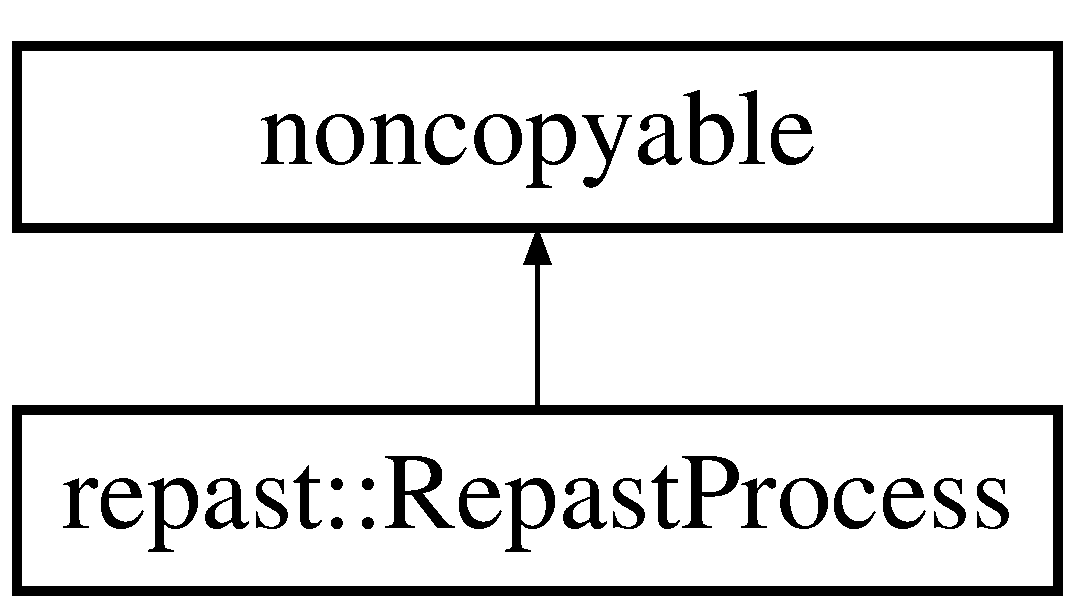
\includegraphics[height=2.000000cm]{classrepast_1_1_repast_process}
\end{center}
\end{figure}
\subsection*{Public Types}
\begin{DoxyCompactItemize}
\item 
enum {\bfseries E\-X\-C\-H\-A\-N\-G\-E\-\_\-\-P\-A\-T\-T\-E\-R\-N} \{ {\bfseries P\-O\-L\-L}, 
{\bfseries U\-S\-E\-\_\-\-C\-U\-R\-R\-E\-N\-T}, 
{\bfseries U\-S\-E\-\_\-\-L\-A\-S\-T\-\_\-\-O\-R\-\_\-\-P\-O\-L\-L}, 
{\bfseries U\-S\-E\-\_\-\-L\-A\-S\-T\-\_\-\-O\-R\-\_\-\-U\-S\-E\-\_\-\-C\-U\-R\-R\-E\-N\-T}
 \}
\end{DoxyCompactItemize}
\subsection*{Public Member Functions}
\begin{DoxyCompactItemize}
\item 
void \hyperlink{classrepast_1_1_repast_process_a20f9086d8f764dea44ddefd157279263}{agent\-Removed} (const \hyperlink{classrepast_1_1_agent_id}{Agent\-Id} \&id)
\begin{DoxyCompactList}\small\item\em N\-O\-N U\-S\-E\-R A\-P\-I. \end{DoxyCompactList}\item 
void \hyperlink{classrepast_1_1_repast_process_a87cced37db3a1810fa4a4beed5c83998}{move\-Agent} (const \hyperlink{classrepast_1_1_agent_id}{Agent\-Id} \&id, int process)
\begin{DoxyCompactList}\small\item\em N\-O\-N U\-S\-E\-R A\-P\-I. \end{DoxyCompactList}\item 
void \hyperlink{classrepast_1_1_repast_process_ab155561fac49d5c7c21a14d385010321}{add\-Exported\-Agent} (int importing\-Process, \hyperlink{classrepast_1_1_agent_id}{Agent\-Id} id)
\begin{DoxyCompactList}\small\item\em N\-O\-N U\-S\-E\-R A\-P\-I. \end{DoxyCompactList}\item 
void \hyperlink{classrepast_1_1_repast_process_a69b8c957acb0d9df24ea37a7d3755e0e}{add\-Imported\-Agent} (\hyperlink{classrepast_1_1_agent_id}{Agent\-Id} id)
\begin{DoxyCompactList}\small\item\em N\-O\-N U\-S\-E\-R A\-P\-I. \end{DoxyCompactList}\item 
int \hyperlink{classrepast_1_1_repast_process_a13b9bbfd146fd534f71c9b7990bab347}{rank} () const 
\begin{DoxyCompactList}\small\item\em Gets the rank of this process. \end{DoxyCompactList}\item 
\hypertarget{classrepast_1_1_repast_process_a7c2aecbb70e0f589d8c458f64f481939}{int \hyperlink{classrepast_1_1_repast_process_a7c2aecbb70e0f589d8c458f64f481939}{world\-Size} () const }\label{classrepast_1_1_repast_process_a7c2aecbb70e0f589d8c458f64f481939}

\begin{DoxyCompactList}\small\item\em Gets the number of processes in the world. \end{DoxyCompactList}\item 
void \hyperlink{classrepast_1_1_repast_process_a410045f31a523ee63f8646d6c7864f94}{done} ()
\begin{DoxyCompactList}\small\item\em Notifes this \hyperlink{classrepast_1_1_repast_process}{Repast\-Process} that simulation has completed. \end{DoxyCompactList}\item 
\hyperlink{classrepast_1_1_schedule_runner}{Schedule\-Runner} \& \hyperlink{classrepast_1_1_repast_process_a056e9a9d3b8383ecd4e223ca30c06817}{get\-Schedule\-Runner} ()
\begin{DoxyCompactList}\small\item\em Gets the \hyperlink{classrepast_1_1_schedule_runner}{Schedule\-Runner} used by this \hyperlink{classrepast_1_1_repast_process}{Repast\-Process}. \end{DoxyCompactList}\item 
\hypertarget{classrepast_1_1_repast_process_a14059c959e8a213bb30c7b414a750ab1}{boost\-::mpi\-::communicator $\ast$ {\bfseries get\-Communicator} ()}\label{classrepast_1_1_repast_process_a14059c959e8a213bb30c7b414a750ab1}

\item 
\hypertarget{classrepast_1_1_repast_process_ae7d551a0294b78c4ebef1de65d7c487e}{void {\bfseries drop\-Importer\-Exporter\-Set} (std\-::string set\-Name)}\label{classrepast_1_1_repast_process_ae7d551a0294b78c4ebef1de65d7c487e}

\item 
\hypertarget{classrepast_1_1_repast_process_a6669a34592bf26e54318bff225be0bc2}{std\-::string {\bfseries Importer\-Exporter\-Version} ()}\label{classrepast_1_1_repast_process_a6669a34592bf26e54318bff225be0bc2}

\item 
\hypertarget{classrepast_1_1_repast_process_a9d747e852bb67271b3d50b311d0ab57c}{std\-::string {\bfseries Importer\-Exporter\-Report} ()}\label{classrepast_1_1_repast_process_a9d747e852bb67271b3d50b311d0ab57c}

\item 
{\footnotesize template$<$typename T , typename Content , typename Provider , typename Updater , typename Agent\-Creator $>$ }\\void \hyperlink{classrepast_1_1_repast_process_af295e322c0902a49ce530fc907b698d3}{request\-Agents} (\hyperlink{classrepast_1_1_shared_context}{Shared\-Context}$<$ T $>$ \&context, \hyperlink{classrepast_1_1_agent_request}{Agent\-Request} \&request, Provider \&provider, Updater \&updater, Agent\-Creator \&creator, std\-::string set\-Name=D\-E\-F\-A\-U\-L\-T\-\_\-\-A\-G\-E\-N\-T\-\_\-\-R\-E\-Q\-U\-E\-S\-T\-\_\-\-S\-E\-T, A\-G\-E\-N\-T\-\_\-\-I\-M\-P\-O\-R\-T\-E\-R\-\_\-\-E\-X\-P\-O\-R\-T\-E\-R\-\_\-\-T\-Y\-P\-E set\-Type=D\-E\-F\-A\-U\-L\-T\-\_\-\-E\-N\-U\-M\-\_\-\-S\-Y\-M\-B\-O\-L)
\begin{DoxyCompactList}\small\item\em Request agents from other processes. \end{DoxyCompactList}\item 
{\footnotesize template$<$typename Content , typename Provider , typename Updater $>$ }\\void \hyperlink{classrepast_1_1_repast_process_a6bf1b59d9939755fedc53264fdb335db}{synchronize\-Agent\-States} (Provider \&provider, Updater \&updater, std\-::string set\-Name=R\-E\-Q\-U\-E\-S\-T\-\_\-\-A\-G\-E\-N\-T\-S\-\_\-\-A\-L\-L)
\begin{DoxyCompactList}\small\item\em Synchronizes the state values of shared agents. \end{DoxyCompactList}\item 
\hypertarget{classrepast_1_1_repast_process_ac630e9787be913cb1101fcba3d6c60a7}{{\footnotesize template$<$typename T , typename Content , typename Provider , typename Updater , typename Agent\-Creator $>$ }\\void \hyperlink{classrepast_1_1_repast_process_ac630e9787be913cb1101fcba3d6c60a7}{synchronize\-Projection\-Info} (\hyperlink{classrepast_1_1_shared_context}{Shared\-Context}$<$ T $>$ \&context, Provider \&provider, Updater \&updater, Agent\-Creator \&creator, E\-X\-C\-H\-A\-N\-G\-E\-\_\-\-P\-A\-T\-T\-E\-R\-N exchange\-Pattern=P\-O\-L\-L, bool declare\-No\-Agents\-Kept\-On\-Any\-Process=false)}\label{classrepast_1_1_repast_process_ac630e9787be913cb1101fcba3d6c60a7}

\begin{DoxyCompactList}\small\item\em Synchronizes the \hyperlink{classrepast_1_1_projection}{Projection} information for shared projections. \end{DoxyCompactList}\item 
{\footnotesize template$<$typename T , typename Content , typename Provider , typename Agent\-Creator , typename Updater $>$ }\\void \hyperlink{classrepast_1_1_repast_process_a243aed166431493c78de8f1f98713743}{synchronize\-Agent\-Status} (\hyperlink{classrepast_1_1_shared_context}{Shared\-Context}$<$ T $>$ \&context, Provider \&provider, Updater \&updater, Agent\-Creator \&creator, E\-X\-C\-H\-A\-N\-G\-E\-\_\-\-P\-A\-T\-T\-E\-R\-N exchange\-Pattern=P\-O\-L\-L)
\begin{DoxyCompactList}\small\item\em Synchronizes the status (moved or died) of all agents across processes. \end{DoxyCompactList}\end{DoxyCompactItemize}
\subsection*{Static Public Member Functions}
\begin{DoxyCompactItemize}
\item 
static \hyperlink{classrepast_1_1_repast_process}{Repast\-Process} $\ast$ \hyperlink{classrepast_1_1_repast_process_a157a6c1057a1b2fa1d37b8391509611c}{init} (std\-::string propsfile, boost\-::mpi\-::communicator $\ast$comm=0, int max\-Config\-File\-Size=M\-A\-X\-\_\-\-C\-O\-N\-F\-I\-G\-\_\-\-F\-I\-L\-E\-\_\-\-S\-I\-Z\-E)
\begin{DoxyCompactList}\small\item\em Initialize this \hyperlink{classrepast_1_1_repast_process}{Repast\-Process}. \end{DoxyCompactList}\item 
static \hyperlink{classrepast_1_1_repast_process}{Repast\-Process} $\ast$ \hyperlink{classrepast_1_1_repast_process_a8eed21e917ec5d66a11cde664938e92f}{instance} ()
\begin{DoxyCompactList}\small\item\em Gets this \hyperlink{classrepast_1_1_repast_process}{Repast\-Process}. \end{DoxyCompactList}\item 
\hypertarget{classrepast_1_1_repast_process_a117dc528a5c1798163afab08dfdbe335}{static boost\-::mpi\-::communicator $\ast$ {\bfseries communicator} ()}\label{classrepast_1_1_repast_process_a117dc528a5c1798163afab08dfdbe335}

\end{DoxyCompactItemize}
\subsection*{Protected Member Functions}
\begin{DoxyCompactItemize}
\item 
\hypertarget{classrepast_1_1_repast_process_ac225915589d363067d8753dbe9554783}{{\bfseries Repast\-Process} (boost\-::mpi\-::communicator $\ast$comm=0)}\label{classrepast_1_1_repast_process_ac225915589d363067d8753dbe9554783}

\item 
\hypertarget{classrepast_1_1_repast_process_a731b20e6292df4bc8a2d66e9d8f7919d}{void {\bfseries save\-Proj\-Info\-S\-R\-Procs} (std\-::vector$<$ int $>$ \&sends, std\-::vector$<$ int $>$ \&recvs)}\label{classrepast_1_1_repast_process_a731b20e6292df4bc8a2d66e9d8f7919d}

\item 
\hypertarget{classrepast_1_1_repast_process_a57d4b598104de5ac4f9048770b0d86be}{void {\bfseries save\-Agent\-Status\-Info\-S\-R\-Procs} (std\-::vector$<$ int $>$ \&sends, std\-::vector$<$ int $>$ \&recvs)}\label{classrepast_1_1_repast_process_a57d4b598104de5ac4f9048770b0d86be}

\end{DoxyCompactItemize}


\subsection{Detailed Description}
Encapsulates the process in which repast is running and manages interprocess communication etc. 

This is singleton to insure that there is one per actual process. 

\subsection{Member Function Documentation}
\hypertarget{classrepast_1_1_repast_process_ab155561fac49d5c7c21a14d385010321}{\index{repast\-::\-Repast\-Process@{repast\-::\-Repast\-Process}!add\-Exported\-Agent@{add\-Exported\-Agent}}
\index{add\-Exported\-Agent@{add\-Exported\-Agent}!repast::RepastProcess@{repast\-::\-Repast\-Process}}
\subsubsection[{add\-Exported\-Agent}]{\setlength{\rightskip}{0pt plus 5cm}void repast\-::\-Repast\-Process\-::add\-Exported\-Agent (
\begin{DoxyParamCaption}
\item[{int}]{importing\-Process, }
\item[{{\bf Agent\-Id}}]{id}
\end{DoxyParamCaption}
)}}\label{classrepast_1_1_repast_process_ab155561fac49d5c7c21a14d385010321}


N\-O\-N U\-S\-E\-R A\-P\-I. 

Notifies this \hyperlink{classrepast_1_1_repast_process}{Repast\-Process} that it is exporting the specified agent to the specified process. This sort of notification is done automatically when requesting agents, but agents may get added in other ways. \hypertarget{classrepast_1_1_repast_process_a69b8c957acb0d9df24ea37a7d3755e0e}{\index{repast\-::\-Repast\-Process@{repast\-::\-Repast\-Process}!add\-Imported\-Agent@{add\-Imported\-Agent}}
\index{add\-Imported\-Agent@{add\-Imported\-Agent}!repast::RepastProcess@{repast\-::\-Repast\-Process}}
\subsubsection[{add\-Imported\-Agent}]{\setlength{\rightskip}{0pt plus 5cm}void repast\-::\-Repast\-Process\-::add\-Imported\-Agent (
\begin{DoxyParamCaption}
\item[{{\bf Agent\-Id}}]{id}
\end{DoxyParamCaption}
)}}\label{classrepast_1_1_repast_process_a69b8c957acb0d9df24ea37a7d3755e0e}


N\-O\-N U\-S\-E\-R A\-P\-I. 

Notifies this \hyperlink{classrepast_1_1_repast_process}{Repast\-Process} that it is importing the specified agent. This sort of notification is normally done automatically when requesting agents, but imports can occur in other ways. \hypertarget{classrepast_1_1_repast_process_a20f9086d8f764dea44ddefd157279263}{\index{repast\-::\-Repast\-Process@{repast\-::\-Repast\-Process}!agent\-Removed@{agent\-Removed}}
\index{agent\-Removed@{agent\-Removed}!repast::RepastProcess@{repast\-::\-Repast\-Process}}
\subsubsection[{agent\-Removed}]{\setlength{\rightskip}{0pt plus 5cm}void repast\-::\-Repast\-Process\-::agent\-Removed (
\begin{DoxyParamCaption}
\item[{const {\bf Agent\-Id} \&}]{id}
\end{DoxyParamCaption}
)}}\label{classrepast_1_1_repast_process_a20f9086d8f764dea44ddefd157279263}


N\-O\-N U\-S\-E\-R A\-P\-I. 

Notifies this \hyperlink{classrepast_1_1_repast_process}{Repast\-Process} that the specified agent has been removed (e.\-g. the agent \char`\"{}died\char`\"{}). \hypertarget{classrepast_1_1_repast_process_a410045f31a523ee63f8646d6c7864f94}{\index{repast\-::\-Repast\-Process@{repast\-::\-Repast\-Process}!done@{done}}
\index{done@{done}!repast::RepastProcess@{repast\-::\-Repast\-Process}}
\subsubsection[{done}]{\setlength{\rightskip}{0pt plus 5cm}void repast\-::\-Repast\-Process\-::done (
\begin{DoxyParamCaption}
{}
\end{DoxyParamCaption}
)}}\label{classrepast_1_1_repast_process_a410045f31a523ee63f8646d6c7864f94}


Notifes this \hyperlink{classrepast_1_1_repast_process}{Repast\-Process} that simulation has completed. 

This should be called when the simulation has completed. \hypertarget{classrepast_1_1_repast_process_a056e9a9d3b8383ecd4e223ca30c06817}{\index{repast\-::\-Repast\-Process@{repast\-::\-Repast\-Process}!get\-Schedule\-Runner@{get\-Schedule\-Runner}}
\index{get\-Schedule\-Runner@{get\-Schedule\-Runner}!repast::RepastProcess@{repast\-::\-Repast\-Process}}
\subsubsection[{get\-Schedule\-Runner}]{\setlength{\rightskip}{0pt plus 5cm}{\bf Schedule\-Runner}\& repast\-::\-Repast\-Process\-::get\-Schedule\-Runner (
\begin{DoxyParamCaption}
{}
\end{DoxyParamCaption}
)\hspace{0.3cm}{\ttfamily [inline]}}}\label{classrepast_1_1_repast_process_a056e9a9d3b8383ecd4e223ca30c06817}


Gets the \hyperlink{classrepast_1_1_schedule_runner}{Schedule\-Runner} used by this \hyperlink{classrepast_1_1_repast_process}{Repast\-Process}. 

\begin{DoxyReturn}{Returns}
the \hyperlink{classrepast_1_1_schedule_runner}{Schedule\-Runner} used by this \hyperlink{classrepast_1_1_repast_process}{Repast\-Process}. 
\end{DoxyReturn}
\hypertarget{classrepast_1_1_repast_process_a157a6c1057a1b2fa1d37b8391509611c}{\index{repast\-::\-Repast\-Process@{repast\-::\-Repast\-Process}!init@{init}}
\index{init@{init}!repast::RepastProcess@{repast\-::\-Repast\-Process}}
\subsubsection[{init}]{\setlength{\rightskip}{0pt plus 5cm}{\bf Repast\-Process} $\ast$ repast\-::\-Repast\-Process\-::init (
\begin{DoxyParamCaption}
\item[{std\-::string}]{propsfile, }
\item[{boost\-::mpi\-::communicator $\ast$}]{comm = {\ttfamily 0}, }
\item[{int}]{max\-Config\-File\-Size = {\ttfamily MAX\-\_\-CONFIG\-\_\-FILE\-\_\-SIZE}}
\end{DoxyParamCaption}
)\hspace{0.3cm}{\ttfamily [static]}}}\label{classrepast_1_1_repast_process_a157a6c1057a1b2fa1d37b8391509611c}


Initialize this \hyperlink{classrepast_1_1_repast_process}{Repast\-Process}. 

This must be called before the \hyperlink{classrepast_1_1_repast_process}{Repast\-Process} is used. If a configuration properties file is specified this properties file will be used to configure logging.


\begin{DoxyParams}{Parameters}
{\em propsfile} & a configuration properties file. This can be an empty string. \\
\hline
\end{DoxyParams}
\hypertarget{classrepast_1_1_repast_process_a8eed21e917ec5d66a11cde664938e92f}{\index{repast\-::\-Repast\-Process@{repast\-::\-Repast\-Process}!instance@{instance}}
\index{instance@{instance}!repast::RepastProcess@{repast\-::\-Repast\-Process}}
\subsubsection[{instance}]{\setlength{\rightskip}{0pt plus 5cm}{\bf Repast\-Process} $\ast$ repast\-::\-Repast\-Process\-::instance (
\begin{DoxyParamCaption}
{}
\end{DoxyParamCaption}
)\hspace{0.3cm}{\ttfamily [static]}}}\label{classrepast_1_1_repast_process_a8eed21e917ec5d66a11cde664938e92f}


Gets this \hyperlink{classrepast_1_1_repast_process}{Repast\-Process}. 

\begin{DoxyReturn}{Returns}
this \hyperlink{classrepast_1_1_repast_process}{Repast\-Process} instance. 
\end{DoxyReturn}
\hypertarget{classrepast_1_1_repast_process_a87cced37db3a1810fa4a4beed5c83998}{\index{repast\-::\-Repast\-Process@{repast\-::\-Repast\-Process}!move\-Agent@{move\-Agent}}
\index{move\-Agent@{move\-Agent}!repast::RepastProcess@{repast\-::\-Repast\-Process}}
\subsubsection[{move\-Agent}]{\setlength{\rightskip}{0pt plus 5cm}void repast\-::\-Repast\-Process\-::move\-Agent (
\begin{DoxyParamCaption}
\item[{const {\bf Agent\-Id} \&}]{id, }
\item[{int}]{process}
\end{DoxyParamCaption}
)}}\label{classrepast_1_1_repast_process_a87cced37db3a1810fa4a4beed5c83998}


N\-O\-N U\-S\-E\-R A\-P\-I. 

Notifies this \hyperlink{classrepast_1_1_repast_process}{Repast\-Process} that the specified agent should be moved from this process to the specified process.


\begin{DoxyParams}{Parameters}
{\em id} & the id of the agent to be moved \\
\hline
{\em process} & the process to move the agent to \\
\hline
\end{DoxyParams}
\hypertarget{classrepast_1_1_repast_process_a13b9bbfd146fd534f71c9b7990bab347}{\index{repast\-::\-Repast\-Process@{repast\-::\-Repast\-Process}!rank@{rank}}
\index{rank@{rank}!repast::RepastProcess@{repast\-::\-Repast\-Process}}
\subsubsection[{rank}]{\setlength{\rightskip}{0pt plus 5cm}int repast\-::\-Repast\-Process\-::rank (
\begin{DoxyParamCaption}
{}
\end{DoxyParamCaption}
) const\hspace{0.3cm}{\ttfamily [inline]}}}\label{classrepast_1_1_repast_process_a13b9bbfd146fd534f71c9b7990bab347}


Gets the rank of this process. 

\begin{DoxyReturn}{Returns}
the rank of this process. 
\end{DoxyReturn}
\hypertarget{classrepast_1_1_repast_process_af295e322c0902a49ce530fc907b698d3}{\index{repast\-::\-Repast\-Process@{repast\-::\-Repast\-Process}!request\-Agents@{request\-Agents}}
\index{request\-Agents@{request\-Agents}!repast::RepastProcess@{repast\-::\-Repast\-Process}}
\subsubsection[{request\-Agents}]{\setlength{\rightskip}{0pt plus 5cm}template$<$typename T , typename Content , typename Provider , typename Updater , typename Agent\-Creator $>$ void repast\-::\-Repast\-Process\-::request\-Agents (
\begin{DoxyParamCaption}
\item[{{\bf Shared\-Context}$<$ T $>$ \&}]{context, }
\item[{{\bf Agent\-Request} \&}]{request, }
\item[{Provider \&}]{provider, }
\item[{Updater \&}]{updater, }
\item[{Agent\-Creator \&}]{creator, }
\item[{std\-::string}]{set\-Name = {\ttfamily DEFAULT\-\_\-AGENT\-\_\-REQUEST\-\_\-SET}, }
\item[{A\-G\-E\-N\-T\-\_\-\-I\-M\-P\-O\-R\-T\-E\-R\-\_\-\-E\-X\-P\-O\-R\-T\-E\-R\-\_\-\-T\-Y\-P\-E}]{set\-Type = {\ttfamily DEFAULT\-\_\-ENUM\-\_\-SYMBOL}}
\end{DoxyParamCaption}
)}}\label{classrepast_1_1_repast_process_af295e322c0902a49ce530fc907b698d3}


Request agents from other processes. 

Requests agents from one process to others.

Copies of the requested agents' Content are retrieved from their respective processes, created using the Agent\-Creator and added to the specified context.


\begin{DoxyParams}{Parameters}
{\em context} & the context to which the requested agents will be added \\
\hline
{\em request} & the \hyperlink{classrepast_1_1_agent_request}{Agent\-Request} containing the ids of the requested agents \\
\hline
{\em provider} & provides Content for a given an \hyperlink{classrepast_1_1_agent_request}{Agent\-Request} \\
\hline
{\em creator} & creates agents of type T given Content.\\
\hline
\end{DoxyParams}

\begin{DoxyTemplParams}{Template Parameters}
{\em T} & the type of the agents in the context \\
\hline
{\em Content} & the serializable struct or class that describes the state of agents \\
\hline
{\em Provider} & given an \hyperlink{classrepast_1_1_agent_request}{Agent\-Request}, a Provider provides the Content for the requested agents, implementing void provide\-Content(const \hyperlink{classrepast_1_1_agent_request}{Agent\-Request}\&, std\-::vector$<$\-Content$>$\&) \\
\hline
{\em Agent\-Creator} & a class that can create agents from Content, implementing T$\ast$ create\-Agent(\-Content\&). \\
\hline
\end{DoxyTemplParams}
\hypertarget{classrepast_1_1_repast_process_a6bf1b59d9939755fedc53264fdb335db}{\index{repast\-::\-Repast\-Process@{repast\-::\-Repast\-Process}!synchronize\-Agent\-States@{synchronize\-Agent\-States}}
\index{synchronize\-Agent\-States@{synchronize\-Agent\-States}!repast::RepastProcess@{repast\-::\-Repast\-Process}}
\subsubsection[{synchronize\-Agent\-States}]{\setlength{\rightskip}{0pt plus 5cm}template$<$typename Content , typename Provider , typename Updater $>$ void repast\-::\-Repast\-Process\-::synchronize\-Agent\-States (
\begin{DoxyParamCaption}
\item[{Provider \&}]{provider, }
\item[{Updater \&}]{updater, }
\item[{std\-::string}]{set\-Name = {\ttfamily REQUEST\-\_\-AGENTS\-\_\-ALL}}
\end{DoxyParamCaption}
)}}\label{classrepast_1_1_repast_process_a6bf1b59d9939755fedc53264fdb335db}


Synchronizes the state values of shared agents. 

Does not change the \hyperlink{classrepast_1_1_projection}{Projection} information for those agents. \hypertarget{classrepast_1_1_repast_process_a243aed166431493c78de8f1f98713743}{\index{repast\-::\-Repast\-Process@{repast\-::\-Repast\-Process}!synchronize\-Agent\-Status@{synchronize\-Agent\-Status}}
\index{synchronize\-Agent\-Status@{synchronize\-Agent\-Status}!repast::RepastProcess@{repast\-::\-Repast\-Process}}
\subsubsection[{synchronize\-Agent\-Status}]{\setlength{\rightskip}{0pt plus 5cm}template$<$typename T , typename Content , typename Provider , typename Agent\-Creator , typename Updater $>$ void repast\-::\-Repast\-Process\-::synchronize\-Agent\-Status (
\begin{DoxyParamCaption}
\item[{{\bf Shared\-Context}$<$ T $>$ \&}]{context, }
\item[{Provider \&}]{provider, }
\item[{Updater \&}]{updater, }
\item[{Agent\-Creator \&}]{creator, }
\item[{E\-X\-C\-H\-A\-N\-G\-E\-\_\-\-P\-A\-T\-T\-E\-R\-N}]{exchange\-Pattern = {\ttfamily POLL}}
\end{DoxyParamCaption}
)}}\label{classrepast_1_1_repast_process_a243aed166431493c78de8f1f98713743}


Synchronizes the status (moved or died) of all agents across processes. 


\begin{DoxyParams}{Parameters}
{\em context} & the \hyperlink{classrepast_1_1_shared_context}{Shared\-Context} that contains the agents on this proceses \\
\hline
{\em provider} & the class that provides agents given an \hyperlink{classrepast_1_1_agent_request}{Agent\-Request} \\
\hline
{\em creator} & creates agents of type T given Content.\\
\hline
\end{DoxyParams}

\begin{DoxyTemplParams}{Template Parameters}
{\em T} & the type of agents in the context \\
\hline
{\em Content} & the serializable struct or class that describes an agents state. \\
\hline
{\em Provider} & a class that provides Content, when given an \hyperlink{classrepast_1_1_agent_request}{Agent\-Request}, implementing void provide\-Content(const repast\-::\-Agent\-Request\&, std\-::vector$<$\-Content$>$\& out) \\
\hline
{\em Agent\-Creator} & a class that can create agents from Content, implementing T$\ast$ create\-Agent(\-Content\&). \\
\hline
\end{DoxyTemplParams}


The documentation for this class was generated from the following files\-:\begin{DoxyCompactItemize}
\item 
repast\-\_\-hpc/Repast\-Process.\-h\item 
repast\-\_\-hpc/Repast\-Process.\-cpp\end{DoxyCompactItemize}

\hypertarget{classrepast_1_1_repeating_event}{\section{repast\-:\-:Repeating\-Event Class Reference}
\label{classrepast_1_1_repeating_event}\index{repast\-::\-Repeating\-Event@{repast\-::\-Repeating\-Event}}
}


\hyperlink{classrepast_1_1_scheduled_event}{Scheduled\-Event} that executes repeatedly.  




{\ttfamily \#include $<$Schedule.\-h$>$}

Inheritance diagram for repast\-:\-:Repeating\-Event\-:\begin{figure}[H]
\begin{center}
\leavevmode
\includegraphics[height=2.000000cm]{classrepast_1_1_repeating_event}
\end{center}
\end{figure}
\subsection*{Public Member Functions}
\begin{DoxyCompactItemize}
\item 
\hypertarget{classrepast_1_1_repeating_event_ae91b8afd1d9213187d47a856ce4094ca}{{\bfseries Repeating\-Event} (double start, double \-\_\-interval, \hyperlink{classrepast_1_1_repast_event}{Repast\-Event} $\ast$)}\label{classrepast_1_1_repeating_event_ae91b8afd1d9213187d47a856ce4094ca}

\item 
\hypertarget{classrepast_1_1_repeating_event_a9ebf48f9a13066db44689b07094f5e39}{virtual bool \hyperlink{classrepast_1_1_repeating_event_a9ebf48f9a13066db44689b07094f5e39}{reschedule} (std\-::priority\-\_\-queue$<$ \hyperlink{classrepast_1_1_scheduled_event}{Scheduled\-Event} $\ast$, std\-::vector$<$ \hyperlink{classrepast_1_1_scheduled_event}{Scheduled\-Event} $\ast$ $>$, \hyperlink{classrepast_1_1_event_compare}{Event\-Compare} $>$ \&)}\label{classrepast_1_1_repeating_event_a9ebf48f9a13066db44689b07094f5e39}

\begin{DoxyCompactList}\small\item\em Returns true if this event is rescheduled on the specified queue, otherwise false. \end{DoxyCompactList}\end{DoxyCompactItemize}
\subsection*{Additional Inherited Members}


\subsection{Detailed Description}
\hyperlink{classrepast_1_1_scheduled_event}{Scheduled\-Event} that executes repeatedly. 

This will reschedule itself repeatedly at the appropriate interval. 

The documentation for this class was generated from the following files\-:\begin{DoxyCompactItemize}
\item 
repast\-\_\-hpc/Schedule.\-h\item 
repast\-\_\-hpc/Schedule.\-cpp\end{DoxyCompactItemize}

\hypertarget{classrepast_1_1_request___packet}{\section{repast\-:\-:Request\-\_\-\-Packet$<$ Content $>$ Class Template Reference}
\label{classrepast_1_1_request___packet}\index{repast\-::\-Request\-\_\-\-Packet$<$ Content $>$@{repast\-::\-Request\-\_\-\-Packet$<$ Content $>$}}
}


Contains information sent as agents are exchanged, either in response to requests or agent movement.  




{\ttfamily \#include $<$Repast\-Process.\-h$>$}

\subsection*{Public Member Functions}
\begin{DoxyCompactItemize}
\item 
\hypertarget{classrepast_1_1_request___packet_a533d224a16012ea64470f1dbb62877d2}{{\bfseries Request\-\_\-\-Packet} (std\-::vector$<$ Content $>$ $\ast$agent\-Content, std\-::map$<$ std\-::string, std\-::vector$<$ \hyperlink{classrepast_1_1_projection_info_packet}{Projection\-Info\-Packet} $\ast$ $>$ $>$ $\ast$projection\-Info)}\label{classrepast_1_1_request___packet_a533d224a16012ea64470f1dbb62877d2}

\item 
\hypertarget{classrepast_1_1_request___packet_abb795210d8ed989db6c0f03a74883751}{{\footnotesize template$<$class Archive $>$ }\\void {\bfseries serialize} (Archive \&ar, const unsigned int version)}\label{classrepast_1_1_request___packet_abb795210d8ed989db6c0f03a74883751}

\end{DoxyCompactItemize}
\subsection*{Public Attributes}
\begin{DoxyCompactItemize}
\item 
\hypertarget{classrepast_1_1_request___packet_a59c95fb4b18c6196f9b2add885b272e1}{std\-::vector$<$ Content $>$ $\ast$ {\bfseries agent\-Content\-Ptr}}\label{classrepast_1_1_request___packet_a59c95fb4b18c6196f9b2add885b272e1}

\item 
\hypertarget{classrepast_1_1_request___packet_aa95c5672630f536c4f4c57c39b78fa1c}{std\-::map$<$ std\-::string, \\*
std\-::vector\\*
$<$ \hyperlink{classrepast_1_1_projection_info_packet}{Projection\-Info\-Packet} $\ast$ $>$ $>$ $\ast$ {\bfseries projection\-Info\-Ptr}}\label{classrepast_1_1_request___packet_aa95c5672630f536c4f4c57c39b78fa1c}

\end{DoxyCompactItemize}
\subsection*{Friends}
\begin{DoxyCompactItemize}
\item 
\hypertarget{classrepast_1_1_request___packet_ac98d07dd8f7b70e16ccb9a01abf56b9c}{class {\bfseries boost\-::serialization\-::access}}\label{classrepast_1_1_request___packet_ac98d07dd8f7b70e16ccb9a01abf56b9c}

\end{DoxyCompactItemize}


\subsection{Detailed Description}
\subsubsection*{template$<$typename Content$>$class repast\-::\-Request\-\_\-\-Packet$<$ Content $>$}

Contains information sent as agents are exchanged, either in response to requests or agent movement. 

Contains both agent raw information (of type 'Content') and projection information.

Note\-: A 'Packet' is responsible for deleting the objects to which it points This is essentially not optional\-: when boost sends the Packet via M\-P\-I the locations at which it places the different elements are not known (no 'new' is called in the user code). Some code must be written to track these down and delete, and it is manifestly easier to provide that code in the Packet itself than to rewrite where needed, inspecting the Packet for the locations 

The documentation for this class was generated from the following file\-:\begin{DoxyCompactItemize}
\item 
repast\-\_\-hpc/Repast\-Process.\-h\end{DoxyCompactItemize}

\hypertarget{class_rolling_file_appender}{\section{Rolling\-File\-Appender Class Reference}
\label{class_rolling_file_appender}\index{Rolling\-File\-Appender@{Rolling\-File\-Appender}}
}
Inheritance diagram for Rolling\-File\-Appender\-:\begin{figure}[H]
\begin{center}
\leavevmode
\includegraphics[height=2.000000cm]{class_rolling_file_appender}
\end{center}
\end{figure}
\subsection*{Public Member Functions}
\begin{DoxyCompactItemize}
\item 
\hypertarget{class_rolling_file_appender_ad064edb9a9a56abe1bb8d2c99551c32f}{{\bfseries Rolling\-File\-Appender} (const string name, const string file\-\_\-name, int max\-\_\-backup, int max\-\_\-size)}\label{class_rolling_file_appender_ad064edb9a9a56abe1bb8d2c99551c32f}

\item 
\hypertarget{class_rolling_file_appender_a8e4a0abe8891bd2e28aa8b39e92c0435}{virtual void {\bfseries write} (const string \&log\-\_\-line)}\label{class_rolling_file_appender_a8e4a0abe8891bd2e28aa8b39e92c0435}

\item 
\hypertarget{class_rolling_file_appender_a123c83a1000ca9cd0f40fe747c816bcc}{virtual void {\bfseries close} ()}\label{class_rolling_file_appender_a123c83a1000ca9cd0f40fe747c816bcc}

\end{DoxyCompactItemize}
\subsection*{Additional Inherited Members}


The documentation for this class was generated from the following file\-:\begin{DoxyCompactItemize}
\item 
repast\-\_\-hpc/logger.\-cpp\end{DoxyCompactItemize}

\hypertarget{classrepast_1_1_schedule}{\section{repast\-:\-:Schedule Class Reference}
\label{classrepast_1_1_schedule}\index{repast\-::\-Schedule@{repast\-::\-Schedule}}
}


The simulation schedule queue.  




{\ttfamily \#include $<$Schedule.\-h$>$}

\subsection*{Public Types}
\begin{DoxyCompactItemize}
\item 
\hypertarget{classrepast_1_1_schedule_a6a31b68f08a9bb28381ffe02b18f1df3}{typedef boost\-::shared\-\_\-ptr\\*
$<$ \hyperlink{classrepast_1_1_functor}{Functor} $>$ \hyperlink{classrepast_1_1_schedule_a6a31b68f08a9bb28381ffe02b18f1df3}{Functor\-Ptr}}\label{classrepast_1_1_schedule_a6a31b68f08a9bb28381ffe02b18f1df3}

\begin{DoxyCompactList}\small\item\em Typedef of for the functors that get scheduled. \end{DoxyCompactList}\end{DoxyCompactItemize}
\subsection*{Public Member Functions}
\begin{DoxyCompactItemize}
\item 
\hyperlink{classrepast_1_1_scheduled_event}{Scheduled\-Event} $\ast$ \hyperlink{classrepast_1_1_schedule_ac5084614d3511d6fae1ccb998be2453f}{schedule\-\_\-event} (double at, \hyperlink{classrepast_1_1_schedule_a6a31b68f08a9bb28381ffe02b18f1df3}{Functor\-Ptr} functor)
\begin{DoxyCompactList}\small\item\em \hyperlink{classrepast_1_1_schedule}{Schedule} the specified functor to execute once at the specified tick. \end{DoxyCompactList}\item 
\hyperlink{classrepast_1_1_scheduled_event}{Scheduled\-Event} $\ast$ \hyperlink{classrepast_1_1_schedule_a31305c3673b85cfa1e7cb3cc5e33acfc}{schedule\-\_\-event} (double start, double interval, \hyperlink{classrepast_1_1_schedule_a6a31b68f08a9bb28381ffe02b18f1df3}{Functor\-Ptr} func)
\begin{DoxyCompactList}\small\item\em Schedules the specified functor to execute start at start, and at the specified interval thereafter. \end{DoxyCompactList}\item 
\hypertarget{classrepast_1_1_schedule_ab055ccbdc3f4d9bb7602704b017f9363}{void {\bfseries execute} ()}\label{classrepast_1_1_schedule_ab055ccbdc3f4d9bb7602704b017f9363}

\item 
double \hyperlink{classrepast_1_1_schedule_a04f76630d4435283b94ee526f4de752b}{get\-Current\-Tick} () const 
\begin{DoxyCompactList}\small\item\em Gets the current simulation tick. \end{DoxyCompactList}\item 
double \hyperlink{classrepast_1_1_schedule_a02063913da3dac3a2f1b71d6dde05bea}{get\-Next\-Tick} () const 
\begin{DoxyCompactList}\small\item\em Gets the next tick at which the next events will be executed. \end{DoxyCompactList}\end{DoxyCompactItemize}


\subsection{Detailed Description}
The simulation schedule queue. 

This wraps a priority queue to schedule repast Scheduled\-Events. 

\subsection{Member Function Documentation}
\hypertarget{classrepast_1_1_schedule_a04f76630d4435283b94ee526f4de752b}{\index{repast\-::\-Schedule@{repast\-::\-Schedule}!get\-Current\-Tick@{get\-Current\-Tick}}
\index{get\-Current\-Tick@{get\-Current\-Tick}!repast::Schedule@{repast\-::\-Schedule}}
\subsubsection[{get\-Current\-Tick}]{\setlength{\rightskip}{0pt plus 5cm}double repast\-::\-Schedule\-::get\-Current\-Tick (
\begin{DoxyParamCaption}
{}
\end{DoxyParamCaption}
) const\hspace{0.3cm}{\ttfamily [inline]}}}\label{classrepast_1_1_schedule_a04f76630d4435283b94ee526f4de752b}


Gets the current simulation tick. 

\begin{DoxyReturn}{Returns}
the current simulation tick. 
\end{DoxyReturn}
\hypertarget{classrepast_1_1_schedule_a02063913da3dac3a2f1b71d6dde05bea}{\index{repast\-::\-Schedule@{repast\-::\-Schedule}!get\-Next\-Tick@{get\-Next\-Tick}}
\index{get\-Next\-Tick@{get\-Next\-Tick}!repast::Schedule@{repast\-::\-Schedule}}
\subsubsection[{get\-Next\-Tick}]{\setlength{\rightskip}{0pt plus 5cm}double repast\-::\-Schedule\-::get\-Next\-Tick (
\begin{DoxyParamCaption}
{}
\end{DoxyParamCaption}
) const\hspace{0.3cm}{\ttfamily [inline]}}}\label{classrepast_1_1_schedule_a02063913da3dac3a2f1b71d6dde05bea}


Gets the next tick at which the next events will be executed. 

\begin{DoxyReturn}{Returns}
the next tick at which the next events will be executed. 
\end{DoxyReturn}
\hypertarget{classrepast_1_1_schedule_ac5084614d3511d6fae1ccb998be2453f}{\index{repast\-::\-Schedule@{repast\-::\-Schedule}!schedule\-\_\-event@{schedule\-\_\-event}}
\index{schedule\-\_\-event@{schedule\-\_\-event}!repast::Schedule@{repast\-::\-Schedule}}
\subsubsection[{schedule\-\_\-event}]{\setlength{\rightskip}{0pt plus 5cm}{\bf Scheduled\-Event} $\ast$ repast\-::\-Schedule\-::schedule\-\_\-event (
\begin{DoxyParamCaption}
\item[{double}]{at, }
\item[{{\bf Functor\-Ptr}}]{functor}
\end{DoxyParamCaption}
)}}\label{classrepast_1_1_schedule_ac5084614d3511d6fae1ccb998be2453f}


\hyperlink{classrepast_1_1_schedule}{Schedule} the specified functor to execute once at the specified tick. 


\begin{DoxyParams}{Parameters}
{\em at} & the tick to execute at \\
\hline
{\em functor} & the functor to schedule\\
\hline
\end{DoxyParams}
\begin{DoxyReturn}{Returns}
the event that has been scheduled 
\end{DoxyReturn}
\hypertarget{classrepast_1_1_schedule_a31305c3673b85cfa1e7cb3cc5e33acfc}{\index{repast\-::\-Schedule@{repast\-::\-Schedule}!schedule\-\_\-event@{schedule\-\_\-event}}
\index{schedule\-\_\-event@{schedule\-\_\-event}!repast::Schedule@{repast\-::\-Schedule}}
\subsubsection[{schedule\-\_\-event}]{\setlength{\rightskip}{0pt plus 5cm}{\bf Scheduled\-Event} $\ast$ repast\-::\-Schedule\-::schedule\-\_\-event (
\begin{DoxyParamCaption}
\item[{double}]{start, }
\item[{double}]{interval, }
\item[{{\bf Functor\-Ptr}}]{func}
\end{DoxyParamCaption}
)}}\label{classrepast_1_1_schedule_a31305c3673b85cfa1e7cb3cc5e33acfc}


Schedules the specified functor to execute start at start, and at the specified interval thereafter. 


\begin{DoxyParams}{Parameters}
{\em start} & \\
\hline
{\em interval} & \\
\hline
{\em func} & \\
\hline
\end{DoxyParams}
\begin{DoxyReturn}{Returns}
the event that has been scheduled 
\end{DoxyReturn}


The documentation for this class was generated from the following files\-:\begin{DoxyCompactItemize}
\item 
repast\-\_\-hpc/Schedule.\-h\item 
repast\-\_\-hpc/Schedule.\-cpp\end{DoxyCompactItemize}

\hypertarget{classrepast_1_1_scheduled_event}{\section{repast\-:\-:Scheduled\-Event Class Reference}
\label{classrepast_1_1_scheduled_event}\index{repast\-::\-Scheduled\-Event@{repast\-::\-Scheduled\-Event}}
}


The object that is placed (scheduled) in the priority queue for execution.  




{\ttfamily \#include $<$Schedule.\-h$>$}

Inheritance diagram for repast\-:\-:Scheduled\-Event\-:\begin{figure}[H]
\begin{center}
\leavevmode
\includegraphics[height=2.000000cm]{classrepast_1_1_scheduled_event}
\end{center}
\end{figure}
\subsection*{Public Member Functions}
\begin{DoxyCompactItemize}
\item 
\hypertarget{classrepast_1_1_scheduled_event_ac2d5b9640a4b968cfc5f94d25ffa1995}{{\bfseries Scheduled\-Event} (double, \hyperlink{classrepast_1_1_repast_event}{Repast\-Event} $\ast$)}\label{classrepast_1_1_scheduled_event_ac2d5b9640a4b968cfc5f94d25ffa1995}

\item 
\hypertarget{classrepast_1_1_scheduled_event_a1fa06003d6e3aecce186ef6eb3e32c61}{virtual bool \hyperlink{classrepast_1_1_scheduled_event_a1fa06003d6e3aecce186ef6eb3e32c61}{reschedule} (std\-::priority\-\_\-queue$<$ \hyperlink{classrepast_1_1_scheduled_event}{Scheduled\-Event} $\ast$, std\-::vector$<$ \hyperlink{classrepast_1_1_scheduled_event}{Scheduled\-Event} $\ast$ $>$, \hyperlink{classrepast_1_1_event_compare}{Event\-Compare} $>$ \&)=0}\label{classrepast_1_1_scheduled_event_a1fa06003d6e3aecce186ef6eb3e32c61}

\begin{DoxyCompactList}\small\item\em Returns true if this event is rescheduled on the specified queue, otherwise false. \end{DoxyCompactList}\item 
\hypertarget{classrepast_1_1_scheduled_event_a937c8e3ec29d6e232201ce9aaffb1e2b}{\hyperlink{classrepast_1_1_repast_event}{Repast\-Event} $\ast$ \hyperlink{classrepast_1_1_scheduled_event_a937c8e3ec29d6e232201ce9aaffb1e2b}{get\-\_\-event} ()}\label{classrepast_1_1_scheduled_event_a937c8e3ec29d6e232201ce9aaffb1e2b}

\begin{DoxyCompactList}\small\item\em Gets the \hyperlink{classrepast_1_1_repast_event}{Repast\-Event} that this Schedule\-Event wraps. \end{DoxyCompactList}\end{DoxyCompactItemize}
\subsection*{Protected Attributes}
\begin{DoxyCompactItemize}
\item 
\hypertarget{classrepast_1_1_scheduled_event_afe1c28943ae16de4fe32ba177741ec70}{\hyperlink{classrepast_1_1_repast_event}{Repast\-Event} $\ast$ {\bfseries event}}\label{classrepast_1_1_scheduled_event_afe1c28943ae16de4fe32ba177741ec70}

\item 
\hypertarget{classrepast_1_1_scheduled_event_a0302155f37ab0345e18e247eb3d3ac16}{double {\bfseries start}}\label{classrepast_1_1_scheduled_event_a0302155f37ab0345e18e247eb3d3ac16}

\end{DoxyCompactItemize}
\subsection*{Friends}
\begin{DoxyCompactItemize}
\item 
\hypertarget{classrepast_1_1_scheduled_event_a13ca8575c9e8e7af0301158bc50424a2}{class {\bfseries Event\-Compare}}\label{classrepast_1_1_scheduled_event_a13ca8575c9e8e7af0301158bc50424a2}

\end{DoxyCompactItemize}


\subsection{Detailed Description}
The object that is placed (scheduled) in the priority queue for execution. 

The documentation for this class was generated from the following files\-:\begin{DoxyCompactItemize}
\item 
repast\-\_\-hpc/Schedule.\-h\item 
repast\-\_\-hpc/Schedule.\-cpp\end{DoxyCompactItemize}

\hypertarget{classrepast_1_1_schedule_runner}{\section{repast\-:\-:Schedule\-Runner Class Reference}
\label{classrepast_1_1_schedule_runner}\index{repast\-::\-Schedule\-Runner@{repast\-::\-Schedule\-Runner}}
}


Runs the \hyperlink{classrepast_1_1_schedule}{Schedule} by popping events off of the \hyperlink{classrepast_1_1_schedule}{Schedule} and executing them; also provides methods for scheduling events.  




{\ttfamily \#include $<$Schedule.\-h$>$}

Inheritance diagram for repast\-:\-:Schedule\-Runner\-:\begin{figure}[H]
\begin{center}
\leavevmode
\includegraphics[height=2.000000cm]{classrepast_1_1_schedule_runner}
\end{center}
\end{figure}
\subsection*{Public Member Functions}
\begin{DoxyCompactItemize}
\item 
\hypertarget{classrepast_1_1_schedule_runner_a160f14417f2400eb2b569edb18ec43f9}{{\bfseries Schedule\-Runner} (boost\-::mpi\-::communicator $\ast$world)}\label{classrepast_1_1_schedule_runner_a160f14417f2400eb2b569edb18ec43f9}

\item 
\hyperlink{classrepast_1_1_scheduled_event}{Scheduled\-Event} $\ast$ \hyperlink{classrepast_1_1_schedule_runner_a607b44e70ad07b8d62cdce1426fb2ddc}{schedule\-Event} (double at, \hyperlink{classrepast_1_1_schedule_a6a31b68f08a9bb28381ffe02b18f1df3}{Schedule\-::\-Functor\-Ptr} func)
\begin{DoxyCompactList}\small\item\em Schedules the \hyperlink{classrepast_1_1_functor}{Functor} to execute at the specified tick. \end{DoxyCompactList}\item 
\hyperlink{classrepast_1_1_scheduled_event}{Scheduled\-Event} $\ast$ \hyperlink{classrepast_1_1_schedule_runner_a7e043ad51b6f5f7eae71d479e0eae471}{schedule\-Event} (double start, double interval, \hyperlink{classrepast_1_1_schedule_a6a31b68f08a9bb28381ffe02b18f1df3}{Schedule\-::\-Functor\-Ptr} func)
\begin{DoxyCompactList}\small\item\em Schedules the \hyperlink{classrepast_1_1_functor}{Functor} to execute at the specified start tick and every interval thereafter. \end{DoxyCompactList}\item 
void \hyperlink{classrepast_1_1_schedule_runner_a52e62ccda4dc3288c90586d91701ed60}{schedule\-End\-Event} (\hyperlink{classrepast_1_1_schedule_a6a31b68f08a9bb28381ffe02b18f1df3}{Schedule\-::\-Functor\-Ptr} func)
\begin{DoxyCompactList}\small\item\em Schedules the specified functor to execute when the simulation ends. \end{DoxyCompactList}\item 
void \hyperlink{classrepast_1_1_schedule_runner_a86fa8a634ef091adeaa43d03b040060f}{schedule\-Stop} (double at)
\begin{DoxyCompactList}\small\item\em Schedules the simulation to stop at the specified tick. \end{DoxyCompactList}\item 
\hypertarget{classrepast_1_1_schedule_runner_afc5cb8954438ed0a9ff665396b2f2994}{void \hyperlink{classrepast_1_1_schedule_runner_afc5cb8954438ed0a9ff665396b2f2994}{run} ()}\label{classrepast_1_1_schedule_runner_afc5cb8954438ed0a9ff665396b2f2994}

\begin{DoxyCompactList}\small\item\em Starts and runs the simulation schedule. \end{DoxyCompactList}\item 
double \hyperlink{classrepast_1_1_schedule_runner_ab463376b173578b8e4e2f6f1ea378bcd}{current\-Tick} ()
\begin{DoxyCompactList}\small\item\em Gets the current tick. \end{DoxyCompactList}\item 
\hypertarget{classrepast_1_1_schedule_runner_a83c18e2030d72c7ae36ccf6a0723d9b8}{void \hyperlink{classrepast_1_1_schedule_runner_a83c18e2030d72c7ae36ccf6a0723d9b8}{stop} ()}\label{classrepast_1_1_schedule_runner_a83c18e2030d72c7ae36ccf6a0723d9b8}

\begin{DoxyCompactList}\small\item\em Stops the simulation. \end{DoxyCompactList}\item 
const \hyperlink{classrepast_1_1_schedule}{Schedule} \& \hyperlink{classrepast_1_1_schedule_runner_a18301612463546255bcd94513be5cc88}{schedule} ()
\begin{DoxyCompactList}\small\item\em Gets the schedule executed by this simulation runner. \end{DoxyCompactList}\end{DoxyCompactItemize}


\subsection{Detailed Description}
Runs the \hyperlink{classrepast_1_1_schedule}{Schedule} by popping events off of the \hyperlink{classrepast_1_1_schedule}{Schedule} and executing them; also provides methods for scheduling events. 

Simulation events should be scheduled for execution using this class which is accessible via \hyperlink{classrepast_1_1_repast_process_a8eed21e917ec5d66a11cde664938e92f}{Repast\-Process\-::instance()}-\/$>$get\-Schedule\-Runner() 

\subsection{Member Function Documentation}
\hypertarget{classrepast_1_1_schedule_runner_ab463376b173578b8e4e2f6f1ea378bcd}{\index{repast\-::\-Schedule\-Runner@{repast\-::\-Schedule\-Runner}!current\-Tick@{current\-Tick}}
\index{current\-Tick@{current\-Tick}!repast::ScheduleRunner@{repast\-::\-Schedule\-Runner}}
\subsubsection[{current\-Tick}]{\setlength{\rightskip}{0pt plus 5cm}double repast\-::\-Schedule\-Runner\-::current\-Tick (
\begin{DoxyParamCaption}
{}
\end{DoxyParamCaption}
)\hspace{0.3cm}{\ttfamily [inline]}}}\label{classrepast_1_1_schedule_runner_ab463376b173578b8e4e2f6f1ea378bcd}


Gets the current tick. 

\begin{DoxyReturn}{Returns}
the current tick 
\end{DoxyReturn}
\hypertarget{classrepast_1_1_schedule_runner_a18301612463546255bcd94513be5cc88}{\index{repast\-::\-Schedule\-Runner@{repast\-::\-Schedule\-Runner}!schedule@{schedule}}
\index{schedule@{schedule}!repast::ScheduleRunner@{repast\-::\-Schedule\-Runner}}
\subsubsection[{schedule}]{\setlength{\rightskip}{0pt plus 5cm}const {\bf Schedule}\& repast\-::\-Schedule\-Runner\-::schedule (
\begin{DoxyParamCaption}
{}
\end{DoxyParamCaption}
)\hspace{0.3cm}{\ttfamily [inline]}}}\label{classrepast_1_1_schedule_runner_a18301612463546255bcd94513be5cc88}


Gets the schedule executed by this simulation runner. 

\begin{DoxyReturn}{Returns}
the schedule used by this simulation runner. 
\end{DoxyReturn}
\hypertarget{classrepast_1_1_schedule_runner_a52e62ccda4dc3288c90586d91701ed60}{\index{repast\-::\-Schedule\-Runner@{repast\-::\-Schedule\-Runner}!schedule\-End\-Event@{schedule\-End\-Event}}
\index{schedule\-End\-Event@{schedule\-End\-Event}!repast::ScheduleRunner@{repast\-::\-Schedule\-Runner}}
\subsubsection[{schedule\-End\-Event}]{\setlength{\rightskip}{0pt plus 5cm}void repast\-::\-Schedule\-Runner\-::schedule\-End\-Event (
\begin{DoxyParamCaption}
\item[{{\bf Schedule\-::\-Functor\-Ptr}}]{func}
\end{DoxyParamCaption}
)}}\label{classrepast_1_1_schedule_runner_a52e62ccda4dc3288c90586d91701ed60}


Schedules the specified functor to execute when the simulation ends. 


\begin{DoxyParams}{Parameters}
{\em func} & the functor to execute when the simulatione ends \\
\hline
\end{DoxyParams}
\hypertarget{classrepast_1_1_schedule_runner_a607b44e70ad07b8d62cdce1426fb2ddc}{\index{repast\-::\-Schedule\-Runner@{repast\-::\-Schedule\-Runner}!schedule\-Event@{schedule\-Event}}
\index{schedule\-Event@{schedule\-Event}!repast::ScheduleRunner@{repast\-::\-Schedule\-Runner}}
\subsubsection[{schedule\-Event}]{\setlength{\rightskip}{0pt plus 5cm}{\bf Scheduled\-Event} $\ast$ repast\-::\-Schedule\-Runner\-::schedule\-Event (
\begin{DoxyParamCaption}
\item[{double}]{at, }
\item[{{\bf Schedule\-::\-Functor\-Ptr}}]{func}
\end{DoxyParamCaption}
)}}\label{classrepast_1_1_schedule_runner_a607b44e70ad07b8d62cdce1426fb2ddc}


Schedules the \hyperlink{classrepast_1_1_functor}{Functor} to execute at the specified tick. 


\begin{DoxyParams}{Parameters}
{\em at} & the time to execute at \\
\hline
{\em func} & the functor to execute\\
\hline
\end{DoxyParams}
\begin{DoxyReturn}{Returns}
the event that was scheduled for the func 
\end{DoxyReturn}
\hypertarget{classrepast_1_1_schedule_runner_a7e043ad51b6f5f7eae71d479e0eae471}{\index{repast\-::\-Schedule\-Runner@{repast\-::\-Schedule\-Runner}!schedule\-Event@{schedule\-Event}}
\index{schedule\-Event@{schedule\-Event}!repast::ScheduleRunner@{repast\-::\-Schedule\-Runner}}
\subsubsection[{schedule\-Event}]{\setlength{\rightskip}{0pt plus 5cm}{\bf Scheduled\-Event} $\ast$ repast\-::\-Schedule\-Runner\-::schedule\-Event (
\begin{DoxyParamCaption}
\item[{double}]{start, }
\item[{double}]{interval, }
\item[{{\bf Schedule\-::\-Functor\-Ptr}}]{func}
\end{DoxyParamCaption}
)}}\label{classrepast_1_1_schedule_runner_a7e043ad51b6f5f7eae71d479e0eae471}


Schedules the \hyperlink{classrepast_1_1_functor}{Functor} to execute at the specified start tick and every interval thereafter. 


\begin{DoxyParams}{Parameters}
{\em start} & the time to start at \\
\hline
{\em interval} & the interval to execute at \\
\hline
{\em func} & the functor to execute\\
\hline
\end{DoxyParams}
\begin{DoxyReturn}{Returns}
the event that was scheduled for the func 
\end{DoxyReturn}
\hypertarget{classrepast_1_1_schedule_runner_a86fa8a634ef091adeaa43d03b040060f}{\index{repast\-::\-Schedule\-Runner@{repast\-::\-Schedule\-Runner}!schedule\-Stop@{schedule\-Stop}}
\index{schedule\-Stop@{schedule\-Stop}!repast::ScheduleRunner@{repast\-::\-Schedule\-Runner}}
\subsubsection[{schedule\-Stop}]{\setlength{\rightskip}{0pt plus 5cm}void repast\-::\-Schedule\-Runner\-::schedule\-Stop (
\begin{DoxyParamCaption}
\item[{double}]{at}
\end{DoxyParamCaption}
)}}\label{classrepast_1_1_schedule_runner_a86fa8a634ef091adeaa43d03b040060f}


Schedules the simulation to stop at the specified tick. 


\begin{DoxyParams}{Parameters}
{\em at} & the tick at which the simulation should stop \\
\hline
\end{DoxyParams}


The documentation for this class was generated from the following files\-:\begin{DoxyCompactItemize}
\item 
repast\-\_\-hpc/Schedule.\-h\item 
repast\-\_\-hpc/Schedule.\-cpp\end{DoxyCompactItemize}

\hypertarget{structrepast_1_1_second_element}{\section{repast\-:\-:Second\-Element$<$ T $>$ Struct Template Reference}
\label{structrepast_1_1_second_element}\index{repast\-::\-Second\-Element$<$ T $>$@{repast\-::\-Second\-Element$<$ T $>$}}
}


Unary function used in the transform\-\_\-iterator that allows context iterators to return the agent maps values.  




{\ttfamily \#include $<$Context.\-h$>$}

Inheritance diagram for repast\-:\-:Second\-Element$<$ T $>$\-:\begin{figure}[H]
\begin{center}
\leavevmode
\includegraphics[height=1.635036cm]{structrepast_1_1_second_element}
\end{center}
\end{figure}
\subsection*{Public Member Functions}
\begin{DoxyCompactItemize}
\item 
\hypertarget{structrepast_1_1_second_element_abb240a7a393d6a8ed72b365159579e15}{boost\-::shared\-\_\-ptr$<$ T $>$ {\bfseries operator()} (const typename boost\-::unordered\-\_\-map$<$ \hyperlink{classrepast_1_1_agent_id}{Agent\-Id}, boost\-::shared\-\_\-ptr$<$ T $>$ $>$\-::value\-\_\-type \&value) const }\label{structrepast_1_1_second_element_abb240a7a393d6a8ed72b365159579e15}

\end{DoxyCompactItemize}


\subsection{Detailed Description}
\subsubsection*{template$<$typename T$>$struct repast\-::\-Second\-Element$<$ T $>$}

Unary function used in the transform\-\_\-iterator that allows context iterators to return the agent maps values. 

The documentation for this struct was generated from the following file\-:\begin{DoxyCompactItemize}
\item 
repast\-\_\-hpc/Context.\-h\end{DoxyCompactItemize}

\hypertarget{classrepast_1_1_shared_base_grid}{\section{repast\-:\-:Shared\-Base\-Grid$<$ T, G\-P\-Transformer, Adder, G\-P\-Type $>$ Class Template Reference}
\label{classrepast_1_1_shared_base_grid}\index{repast\-::\-Shared\-Base\-Grid$<$ T, G\-P\-Transformer, Adder, G\-P\-Type $>$@{repast\-::\-Shared\-Base\-Grid$<$ T, G\-P\-Transformer, Adder, G\-P\-Type $>$}}
}


\hyperlink{classrepast_1_1_grid}{Grid} / Space implementation specialized for the distributed context.  




{\ttfamily \#include $<$Shared\-Base\-Grid.\-h$>$}

Inheritance diagram for repast\-:\-:Shared\-Base\-Grid$<$ T, G\-P\-Transformer, Adder, G\-P\-Type $>$\-:\begin{figure}[H]
\begin{center}
\leavevmode
\includegraphics[height=5.000000cm]{classrepast_1_1_shared_base_grid}
\end{center}
\end{figure}
\subsection*{Public Member Functions}
\begin{DoxyCompactItemize}
\item 
\hypertarget{classrepast_1_1_shared_base_grid_a6e2cf26b8580f27b9f4bda6afb125987}{void {\bfseries balance} ()}\label{classrepast_1_1_shared_base_grid_a6e2cf26b8580f27b9f4bda6afb125987}

\item 
\hyperlink{classrepast_1_1_shared_base_grid_aa9c93cbd1c9d92839fe8d0a24dbf4279}{Shared\-Base\-Grid} (std\-::string \hyperlink{classrepast_1_1_projection_ab60a0ab4f584685780307d7431b61800}{name}, \hyperlink{classrepast_1_1_grid_dimensions}{Grid\-Dimensions} grid\-Dims, std\-::vector$<$ int $>$ process\-Dims, int buffer, boost\-::mpi\-::communicator $\ast$world)
\begin{DoxyCompactList}\small\item\em Creates a Shared\-Grid with the specified name. \end{DoxyCompactList}\item 
\hyperlink{classrepast_1_1_grid_dimensions}{Grid\-Dimensions} \hyperlink{classrepast_1_1_shared_base_grid_a9eb45d3b57a22564ce892de6bd96e84e}{bounds} () const 
\begin{DoxyCompactList}\small\item\em Gets the local bounds of this Shared\-Grid. \end{DoxyCompactList}\item 
virtual const \hyperlink{classrepast_1_1_grid_dimensions}{Grid\-Dimensions} \hyperlink{classrepast_1_1_shared_base_grid_a9ec19652232000368ec1fe98ff47e121}{dimensions} () const 
\begin{DoxyCompactList}\small\item\em Gets the local bounds of this Shared\-Grid. \end{DoxyCompactList}\item 
void \hyperlink{classrepast_1_1_shared_base_grid_a99014d8854b57524c9cd40e9cea0507a}{synch\-Move} ()
\begin{DoxyCompactList}\small\item\em Synchronizes the movement of agents off on one grid and onto another. \end{DoxyCompactList}\item 
void \hyperlink{classrepast_1_1_shared_base_grid_a5703bee6037934b6be70d4f17a6b4d7b}{init\-Synch\-Buffer} (\hyperlink{classrepast_1_1_shared_context}{Shared\-Context}$<$ T $>$ \&context)
\begin{DoxyCompactList}\small\item\em Initializes the synch buffer operation. \end{DoxyCompactList}\item 
virtual bool \hyperlink{classrepast_1_1_shared_base_grid_a480fc6f517d1bb098c7ee47450fba522}{move\-To} (const \hyperlink{classrepast_1_1_agent_id}{Agent\-Id} \&id, const std\-::vector$<$ G\-P\-Type $>$ \&new\-Location)
\begin{DoxyCompactList}\small\item\em Moves the specified agent to the specified location. \end{DoxyCompactList}\item 
virtual bool \hyperlink{classrepast_1_1_shared_base_grid_ab4d74c36e126cffa5638aeaab6c0df85}{move\-To} (const \hyperlink{classrepast_1_1_agent_id}{Agent\-Id} \&id, const \hyperlink{classrepast_1_1_point}{Point}$<$ G\-P\-Type $>$ \&pt)
\begin{DoxyCompactList}\small\item\em Moves the specified agent to the specified point. \end{DoxyCompactList}\item 
\hypertarget{classrepast_1_1_shared_base_grid_ace1d00758e418a574263997e7db2f26a}{virtual void {\bfseries remove\-Agent} (T $\ast$agent)}\label{classrepast_1_1_shared_base_grid_ace1d00758e418a574263997e7db2f26a}

\item 
\hypertarget{classrepast_1_1_shared_base_grid_a810df20298f76741ab58907fb5e20749}{virtual void {\bfseries get\-Required\-Agents} (std\-::set$<$ \hyperlink{classrepast_1_1_agent_id}{Agent\-Id} $>$ \&agents\-To\-Test, std\-::set$<$ \hyperlink{classrepast_1_1_agent_id}{Agent\-Id} $>$ \&agents\-Required)}\label{classrepast_1_1_shared_base_grid_a810df20298f76741ab58907fb5e20749}

\item 
virtual void \hyperlink{classrepast_1_1_shared_base_grid_ab1486e7698288efc1218653d4e5e1e15}{get\-Agents\-To\-Push} (std\-::set$<$ \hyperlink{classrepast_1_1_agent_id}{Agent\-Id} $>$ \&agents\-To\-Test, std\-::map$<$ int, std\-::set$<$ \hyperlink{classrepast_1_1_agent_id}{Agent\-Id} $>$ $>$ \&agents\-To\-Push)
\begin{DoxyCompactList}\small\item\em Given a set of agents, gets the agents that this projection implementation must 'push' to other processes. \end{DoxyCompactList}\item 
virtual void \hyperlink{classrepast_1_1_shared_base_grid_af4323686714c4f6216125db5609c3184}{get\-Info\-Exchange\-Partners} (std\-::set$<$ int $>$ \&ps\-To\-Send\-To, std\-::set$<$ int $>$ \&ps\-To\-Receive\-From)
\begin{DoxyCompactList}\small\item\em Gets the set of processes with which this \hyperlink{classrepast_1_1_projection}{Projection} exchanges projection info. \end{DoxyCompactList}\item 
virtual void \hyperlink{classrepast_1_1_shared_base_grid_a0388d98240eb59548058d3c45da702d7}{get\-Agent\-Status\-Exchange\-Partners} (std\-::set$<$ int $>$ \&ps\-To\-Send\-To, std\-::set$<$ int $>$ \&ps\-To\-Receive\-From)
\begin{DoxyCompactList}\small\item\em Gets the set of processes with which this \hyperlink{classrepast_1_1_projection}{Projection} exchanges agent status info-\/ that is, the set of processes from which agents can move to this one or to which they can move when moving from this one. \end{DoxyCompactList}\item 
\hypertarget{classrepast_1_1_shared_base_grid_abe043188d6e0f7dd350aed6d78c4b98e}{virtual void {\bfseries update\-Projection\-Info} (\hyperlink{classrepast_1_1_projection_info_packet}{Projection\-Info\-Packet} $\ast$pip, \hyperlink{classrepast_1_1_context}{Context}$<$ T $>$ $\ast$context)}\label{classrepast_1_1_shared_base_grid_abe043188d6e0f7dd350aed6d78c4b98e}

\end{DoxyCompactItemize}
\subsection*{Protected Types}
\begin{DoxyCompactItemize}
\item 
\hypertarget{classrepast_1_1_shared_base_grid_afdd62d17e80eb799ba63451b8f78f0ee}{typedef \hyperlink{classrepast_1_1_base_grid}{repast\-::\-Base\-Grid}$<$ T, \\*
\hyperlink{classrepast_1_1_multiple_occupancy}{Multiple\-Occupancy}$<$ T, G\-P\-Type $>$\\*
, G\-P\-Transformer, Adder, G\-P\-Type $>$ {\bfseries Grid\-Base\-Type}}\label{classrepast_1_1_shared_base_grid_afdd62d17e80eb799ba63451b8f78f0ee}

\end{DoxyCompactItemize}
\subsection*{Protected Member Functions}
\begin{DoxyCompactItemize}
\item 
\hypertarget{classrepast_1_1_shared_base_grid_a84acccc25e0e3e21f8d430a36c9d395a}{\hyperlink{classrepast_1_1_grid_dimensions}{Grid\-Dimensions} {\bfseries create\-Send\-Buffer\-Bounds} (\hyperlink{classrepast_1_1_neighbors_a7a695a73b614b849f12fd943329b8bdc}{Neighbors\-::\-Location} location)}\label{classrepast_1_1_shared_base_grid_a84acccc25e0e3e21f8d430a36c9d395a}

\item 
\hypertarget{classrepast_1_1_shared_base_grid_a51922e0249368abd598ead8101088732}{virtual void {\bfseries synch\-Move\-To} (const \hyperlink{classrepast_1_1_agent_id}{Agent\-Id} \&id, const \hyperlink{classrepast_1_1_point}{Point}$<$ G\-P\-Type $>$ \&pt)=0}\label{classrepast_1_1_shared_base_grid_a51922e0249368abd598ead8101088732}

\item 
\hypertarget{classrepast_1_1_shared_base_grid_a0ea39fedf8dcb4acd0c9011d323ca52d}{void {\bfseries get\-Moving\-Agent\-Info} (std\-::map$<$ int, std\-::vector$<$ \hyperlink{classrepast_1_1_agent_id}{Agent\-Id} $>$ $>$ agents\-To\-Move, \hyperlink{classrepast_1_1_grid_move_packets}{Grid\-Move\-Packets}$<$ G\-P\-Type $>$ outgoing)}\label{classrepast_1_1_shared_base_grid_a0ea39fedf8dcb4acd0c9011d323ca52d}

\item 
\hypertarget{classrepast_1_1_shared_base_grid_a96b291d6e5e8ae2a4100704a4af770c2}{bool {\bfseries location\-Is\-In\-Buffer} (\hyperlink{classrepast_1_1_point}{Point}$<$ G\-P\-Type $>$ pt)}\label{classrepast_1_1_shared_base_grid_a96b291d6e5e8ae2a4100704a4af770c2}

\item 
\hypertarget{classrepast_1_1_shared_base_grid_a0510379d3dab88d33d459b6ae063d07d}{bool {\bfseries agent\-Is\-In\-Buffer} (\hyperlink{classrepast_1_1_agent_id}{Agent\-Id} id)}\label{classrepast_1_1_shared_base_grid_a0510379d3dab88d33d459b6ae063d07d}

\end{DoxyCompactItemize}
\subsection*{Protected Attributes}
\begin{DoxyCompactItemize}
\item 
\hypertarget{classrepast_1_1_shared_base_grid_a2e19f6831a277a4df1373920ea57d8eb}{int {\bfseries \-\_\-buffer}}\label{classrepast_1_1_shared_base_grid_a2e19f6831a277a4df1373920ea57d8eb}

\item 
\hypertarget{classrepast_1_1_shared_base_grid_aa9ea56859b5278b0d6bc2bbd8ab4c46b}{\hyperlink{classrepast_1_1_grid_dimensions}{Grid\-Dimensions} {\bfseries local\-Bounds}}\label{classrepast_1_1_shared_base_grid_aa9ea56859b5278b0d6bc2bbd8ab4c46b}

\item 
\hypertarget{classrepast_1_1_shared_base_grid_a204f5c23dd15d124d558140cc1571e7c}{\hyperlink{classrepast_1_1_neighbors}{Neighbors} {\bfseries nghs}}\label{classrepast_1_1_shared_base_grid_a204f5c23dd15d124d558140cc1571e7c}

\item 
\hypertarget{classrepast_1_1_shared_base_grid_aaa8d5d36ce831a360a88c0149f40cd77}{std\-::vector$<$ \hyperlink{classrepast_1_1_agent_id}{Agent\-Id} $>$ {\bfseries buffered}}\label{classrepast_1_1_shared_base_grid_aaa8d5d36ce831a360a88c0149f40cd77}

\item 
\hypertarget{classrepast_1_1_shared_base_grid_a48f63bb491afa1078c8d6598b32b5e3e}{int {\bfseries rank}}\label{classrepast_1_1_shared_base_grid_a48f63bb491afa1078c8d6598b32b5e3e}

\item 
\hypertarget{classrepast_1_1_shared_base_grid_ab9c405f324b799fa0b5fc7472cf6ab49}{boost\-::mpi\-::communicator $\ast$ {\bfseries comm}}\label{classrepast_1_1_shared_base_grid_ab9c405f324b799fa0b5fc7472cf6ab49}

\end{DoxyCompactItemize}


\subsection{Detailed Description}
\subsubsection*{template$<$typename T, typename G\-P\-Transformer, typename Adder, typename G\-P\-Type$>$class repast\-::\-Shared\-Base\-Grid$<$ T, G\-P\-Transformer, Adder, G\-P\-Type $>$}

\hyperlink{classrepast_1_1_grid}{Grid} / Space implementation specialized for the distributed context. 

Each \hyperlink{classrepast_1_1_shared_base_grid}{Shared\-Base\-Grid} of the same name running on different processes is part of a pan process grid. This class manages this local part of the grid and its communication with its process neighbors. Users can specify a buffer size that determines how much of the neighboring grids are visible in this grid. For example, if this grid originates at 0x0 and ends at 3x3, a buffer of 1 would make the locations (4,0), (4,1) (4,2) ... (4,4) and (0,4), (1,4)... (4,4) visible in this grid. The \hyperlink{classrepast_1_1_shared_base_grid}{Shared\-Base\-Grid} takes many template parameters. Default variations of these that define typical grids and spaces are given in Shared\-Grids in Shared\-Space.\-h


\begin{DoxyTemplParams}{Template Parameters}
{\em T} & the type of objects contained by this \hyperlink{classrepast_1_1_base_grid}{Base\-Grid} \\
\hline
{\em G\-P\-Transformer} & transforms cell points according to the topology (e.\-g. periodic) of the \hyperlink{classrepast_1_1_base_grid}{Base\-Grid}. \\
\hline
{\em Adder} & determines how objects are added to the grid from its associated context. \\
\hline
{\em G\-P\-Type} & the coordinate type of the grid point locations. This must be an int or a double. \\
\hline
\end{DoxyTemplParams}


\subsection{Constructor \& Destructor Documentation}
\hypertarget{classrepast_1_1_shared_base_grid_aa9c93cbd1c9d92839fe8d0a24dbf4279}{\index{repast\-::\-Shared\-Base\-Grid@{repast\-::\-Shared\-Base\-Grid}!Shared\-Base\-Grid@{Shared\-Base\-Grid}}
\index{Shared\-Base\-Grid@{Shared\-Base\-Grid}!repast::SharedBaseGrid@{repast\-::\-Shared\-Base\-Grid}}
\subsubsection[{Shared\-Base\-Grid}]{\setlength{\rightskip}{0pt plus 5cm}template$<$typename T , typename G\-P\-Transformer , typename Adder , typename G\-P\-Type $>$ {\bf repast\-::\-Shared\-Base\-Grid}$<$ T, G\-P\-Transformer, Adder, G\-P\-Type $>$\-::{\bf Shared\-Base\-Grid} (
\begin{DoxyParamCaption}
\item[{std\-::string}]{name, }
\item[{{\bf Grid\-Dimensions}}]{grid\-Dims, }
\item[{std\-::vector$<$ int $>$}]{process\-Dims, }
\item[{int}]{buffer, }
\item[{boost\-::mpi\-::communicator $\ast$}]{world}
\end{DoxyParamCaption}
)}}\label{classrepast_1_1_shared_base_grid_aa9c93cbd1c9d92839fe8d0a24dbf4279}


Creates a Shared\-Grid with the specified name. 


\begin{DoxyParams}{Parameters}
{\em name} & the name of this \hyperlink{classrepast_1_1_shared_base_grid}{Shared\-Base\-Grid} \\
\hline
{\em grid\-Dims} & the dimensions of the entire pan-\/process grid \\
\hline
{\em process\-Dims} & the number of processes in each dimension. This must divide evenly into grid\-Dims. \\
\hline
{\em buffer} & the size of the buffer between this part of the pan-\/process grid and its neighbors. \\
\hline
\end{DoxyParams}


\subsection{Member Function Documentation}
\hypertarget{classrepast_1_1_shared_base_grid_a9eb45d3b57a22564ce892de6bd96e84e}{\index{repast\-::\-Shared\-Base\-Grid@{repast\-::\-Shared\-Base\-Grid}!bounds@{bounds}}
\index{bounds@{bounds}!repast::SharedBaseGrid@{repast\-::\-Shared\-Base\-Grid}}
\subsubsection[{bounds}]{\setlength{\rightskip}{0pt plus 5cm}template$<$typename T, typename G\-P\-Transformer, typename Adder, typename G\-P\-Type$>$ {\bf Grid\-Dimensions} {\bf repast\-::\-Shared\-Base\-Grid}$<$ T, G\-P\-Transformer, Adder, G\-P\-Type $>$\-::bounds (
\begin{DoxyParamCaption}
{}
\end{DoxyParamCaption}
) const\hspace{0.3cm}{\ttfamily [inline]}}}\label{classrepast_1_1_shared_base_grid_a9eb45d3b57a22564ce892de6bd96e84e}


Gets the local bounds of this Shared\-Grid. 

The local bounds are the dimensions of the section of the pan-\/process grid represented by this Shared\-Grid.

\begin{DoxyReturn}{Returns}
the local bounds of this Shared\-Grid. 
\end{DoxyReturn}
\hypertarget{classrepast_1_1_shared_base_grid_a9ec19652232000368ec1fe98ff47e121}{\index{repast\-::\-Shared\-Base\-Grid@{repast\-::\-Shared\-Base\-Grid}!dimensions@{dimensions}}
\index{dimensions@{dimensions}!repast::SharedBaseGrid@{repast\-::\-Shared\-Base\-Grid}}
\subsubsection[{dimensions}]{\setlength{\rightskip}{0pt plus 5cm}template$<$typename T, typename G\-P\-Transformer, typename Adder, typename G\-P\-Type$>$ virtual const {\bf Grid\-Dimensions} {\bf repast\-::\-Shared\-Base\-Grid}$<$ T, G\-P\-Transformer, Adder, G\-P\-Type $>$\-::dimensions (
\begin{DoxyParamCaption}
{}
\end{DoxyParamCaption}
) const\hspace{0.3cm}{\ttfamily [inline]}, {\ttfamily [virtual]}}}\label{classrepast_1_1_shared_base_grid_a9ec19652232000368ec1fe98ff47e121}


Gets the local bounds of this Shared\-Grid. 

The local bounds are the dimensions of the section of the pan-\/process grid represented by this Shared\-Grid.

\begin{DoxyReturn}{Returns}
the local bounds of this Shared\-Grid. 
\end{DoxyReturn}


Reimplemented from \hyperlink{classrepast_1_1_base_grid_a5f8a2fc16b8aeba026a58fcb374cf05c}{repast\-::\-Base\-Grid$<$ T, Multiple\-Occupancy$<$ T, G\-P\-Type $>$, G\-P\-Transformer, Adder, G\-P\-Type $>$}.

\hypertarget{classrepast_1_1_shared_base_grid_a0388d98240eb59548058d3c45da702d7}{\index{repast\-::\-Shared\-Base\-Grid@{repast\-::\-Shared\-Base\-Grid}!get\-Agent\-Status\-Exchange\-Partners@{get\-Agent\-Status\-Exchange\-Partners}}
\index{get\-Agent\-Status\-Exchange\-Partners@{get\-Agent\-Status\-Exchange\-Partners}!repast::SharedBaseGrid@{repast\-::\-Shared\-Base\-Grid}}
\subsubsection[{get\-Agent\-Status\-Exchange\-Partners}]{\setlength{\rightskip}{0pt plus 5cm}template$<$typename T, typename G\-P\-Transformer, typename Adder, typename G\-P\-Type$>$ virtual void {\bf repast\-::\-Shared\-Base\-Grid}$<$ T, G\-P\-Transformer, Adder, G\-P\-Type $>$\-::get\-Agent\-Status\-Exchange\-Partners (
\begin{DoxyParamCaption}
\item[{std\-::set$<$ int $>$ \&}]{ps\-To\-Send\-To, }
\item[{std\-::set$<$ int $>$ \&}]{ps\-To\-Receive\-From}
\end{DoxyParamCaption}
)\hspace{0.3cm}{\ttfamily [inline]}, {\ttfamily [virtual]}}}\label{classrepast_1_1_shared_base_grid_a0388d98240eb59548058d3c45da702d7}


Gets the set of processes with which this \hyperlink{classrepast_1_1_projection}{Projection} exchanges agent status info-\/ that is, the set of processes from which agents can move to this one or to which they can move when moving from this one. 

In the most general case this will be all other processors. However, simulations where agents move in spaces will usually exchange agents only with a small subset of 'neighbor' processes, which is knowable in advance and constant. To accommodate the general case, the algorithm for exchanging information must poll all other processes to see which are sending to this one; if this is known in advance, this additional (expensive) step can be skipped. 

Implements \hyperlink{classrepast_1_1_grid_a748354698308fe0d0c0fe33a657109d1}{repast\-::\-Grid$<$ T, G\-P\-Type $>$}.

\hypertarget{classrepast_1_1_shared_base_grid_ab1486e7698288efc1218653d4e5e1e15}{\index{repast\-::\-Shared\-Base\-Grid@{repast\-::\-Shared\-Base\-Grid}!get\-Agents\-To\-Push@{get\-Agents\-To\-Push}}
\index{get\-Agents\-To\-Push@{get\-Agents\-To\-Push}!repast::SharedBaseGrid@{repast\-::\-Shared\-Base\-Grid}}
\subsubsection[{get\-Agents\-To\-Push}]{\setlength{\rightskip}{0pt plus 5cm}template$<$typename T , typename G\-P\-Transformer , typename Adder , typename G\-P\-Type $>$ void {\bf repast\-::\-Shared\-Base\-Grid}$<$ T, G\-P\-Transformer, Adder, G\-P\-Type $>$\-::get\-Agents\-To\-Push (
\begin{DoxyParamCaption}
\item[{std\-::set$<$ {\bf Agent\-Id} $>$ \&}]{agents\-To\-Test, }
\item[{std\-::map$<$ int, std\-::set$<$ {\bf Agent\-Id} $>$ $>$ \&}]{agents\-To\-Push}
\end{DoxyParamCaption}
)\hspace{0.3cm}{\ttfamily [virtual]}}}\label{classrepast_1_1_shared_base_grid_ab1486e7698288efc1218653d4e5e1e15}


Given a set of agents, gets the agents that this projection implementation must 'push' to other processes. 

Generally spaces must push agents that are in 'buffer zones' and graphs must push local agents that are vertices to master edges where the other vertex is non-\/ local. The results are returned per-\/process in the agents\-To\-Push map. 

Reimplemented from \hyperlink{classrepast_1_1_base_grid_a8f718ade5af8285f71151eea824ce3cd}{repast\-::\-Base\-Grid$<$ T, Multiple\-Occupancy$<$ T, G\-P\-Type $>$, G\-P\-Transformer, Adder, G\-P\-Type $>$}.



Reimplemented in \hyperlink{classrepast_1_1_shared_discrete_space_a1f690e82e6b7ea6a279db020e12b4d21}{repast\-::\-Shared\-Discrete\-Space$<$ T, G\-P\-Transformer, Adder $>$}.

\hypertarget{classrepast_1_1_shared_base_grid_af4323686714c4f6216125db5609c3184}{\index{repast\-::\-Shared\-Base\-Grid@{repast\-::\-Shared\-Base\-Grid}!get\-Info\-Exchange\-Partners@{get\-Info\-Exchange\-Partners}}
\index{get\-Info\-Exchange\-Partners@{get\-Info\-Exchange\-Partners}!repast::SharedBaseGrid@{repast\-::\-Shared\-Base\-Grid}}
\subsubsection[{get\-Info\-Exchange\-Partners}]{\setlength{\rightskip}{0pt plus 5cm}template$<$typename T, typename G\-P\-Transformer, typename Adder, typename G\-P\-Type$>$ virtual void {\bf repast\-::\-Shared\-Base\-Grid}$<$ T, G\-P\-Transformer, Adder, G\-P\-Type $>$\-::get\-Info\-Exchange\-Partners (
\begin{DoxyParamCaption}
\item[{std\-::set$<$ int $>$ \&}]{ps\-To\-Send\-To, }
\item[{std\-::set$<$ int $>$ \&}]{ps\-To\-Receive\-From}
\end{DoxyParamCaption}
)\hspace{0.3cm}{\ttfamily [inline]}, {\ttfamily [virtual]}}}\label{classrepast_1_1_shared_base_grid_af4323686714c4f6216125db5609c3184}


Gets the set of processes with which this \hyperlink{classrepast_1_1_projection}{Projection} exchanges projection info. 

In the most general case this will be all other processors; this is the case for graphs, where agent connections can be arbitrary. However, spaces usually exchange information only with a small subset of 'neighbor' processes, which is knowable in advance and constant. To accommodate the general case, the algorithm for exchanging information must poll all other processes to see which are sending to this one; if this is known in advance, this additional (expensive) step can be skipped. 

Implements \hyperlink{classrepast_1_1_grid_a57b4449e602392119eb4db3e0011de05}{repast\-::\-Grid$<$ T, G\-P\-Type $>$}.

\hypertarget{classrepast_1_1_shared_base_grid_a5703bee6037934b6be70d4f17a6b4d7b}{\index{repast\-::\-Shared\-Base\-Grid@{repast\-::\-Shared\-Base\-Grid}!init\-Synch\-Buffer@{init\-Synch\-Buffer}}
\index{init\-Synch\-Buffer@{init\-Synch\-Buffer}!repast::SharedBaseGrid@{repast\-::\-Shared\-Base\-Grid}}
\subsubsection[{init\-Synch\-Buffer}]{\setlength{\rightskip}{0pt plus 5cm}template$<$typename T, typename G\-P\-Transformer , typename Adder , typename G\-P\-Type $>$ void {\bf repast\-::\-Shared\-Base\-Grid}$<$ T, G\-P\-Transformer, Adder, G\-P\-Type $>$\-::init\-Synch\-Buffer (
\begin{DoxyParamCaption}
\item[{{\bf Shared\-Context}$<$ T $>$ \&}]{context}
\end{DoxyParamCaption}
)}}\label{classrepast_1_1_shared_base_grid_a5703bee6037934b6be70d4f17a6b4d7b}


Initializes the synch buffer operation. 

This should be called before synchronizing the buffers themselves.


\begin{DoxyParams}{Parameters}
{\em the} & \hyperlink{classrepast_1_1_shared_context}{Shared\-Context} that contains this Shared\-Grid projection. \\
\hline
\end{DoxyParams}
\hypertarget{classrepast_1_1_shared_base_grid_a480fc6f517d1bb098c7ee47450fba522}{\index{repast\-::\-Shared\-Base\-Grid@{repast\-::\-Shared\-Base\-Grid}!move\-To@{move\-To}}
\index{move\-To@{move\-To}!repast::SharedBaseGrid@{repast\-::\-Shared\-Base\-Grid}}
\subsubsection[{move\-To}]{\setlength{\rightskip}{0pt plus 5cm}template$<$typename T , typename G\-P\-Transformer , typename Adder , typename G\-P\-Type$>$ bool {\bf repast\-::\-Shared\-Base\-Grid}$<$ T, G\-P\-Transformer, Adder, G\-P\-Type $>$\-::move\-To (
\begin{DoxyParamCaption}
\item[{const {\bf Agent\-Id} \&}]{id, }
\item[{const std\-::vector$<$ G\-P\-Type $>$ \&}]{new\-Location}
\end{DoxyParamCaption}
)\hspace{0.3cm}{\ttfamily [virtual]}}}\label{classrepast_1_1_shared_base_grid_a480fc6f517d1bb098c7ee47450fba522}


Moves the specified agent to the specified location. 

Returns true if the move was successful otherwise false. The agent must be already added to the context associated with this space, otherwise this throws an out\-\_\-of\-\_\-range exception if the new location out of bounds.


\begin{DoxyParams}{Parameters}
{\em id} & the id of the agent to move \\
\hline
{\em new\-Location} & the location to move to\\
\hline
\end{DoxyParams}
\begin{DoxyReturn}{Returns}
true if the move was successful, otherwise false 
\end{DoxyReturn}


Reimplemented from \hyperlink{classrepast_1_1_base_grid_a3a39996218f4426aa1b2f081d3b44eb4}{repast\-::\-Base\-Grid$<$ T, Multiple\-Occupancy$<$ T, G\-P\-Type $>$, G\-P\-Transformer, Adder, G\-P\-Type $>$}.

\hypertarget{classrepast_1_1_shared_base_grid_ab4d74c36e126cffa5638aeaab6c0df85}{\index{repast\-::\-Shared\-Base\-Grid@{repast\-::\-Shared\-Base\-Grid}!move\-To@{move\-To}}
\index{move\-To@{move\-To}!repast::SharedBaseGrid@{repast\-::\-Shared\-Base\-Grid}}
\subsubsection[{move\-To}]{\setlength{\rightskip}{0pt plus 5cm}template$<$typename T , typename G\-P\-Transformer , typename Adder , typename G\-P\-Type$>$ bool {\bf repast\-::\-Shared\-Base\-Grid}$<$ T, G\-P\-Transformer, Adder, G\-P\-Type $>$\-::move\-To (
\begin{DoxyParamCaption}
\item[{const {\bf Agent\-Id} \&}]{id, }
\item[{const {\bf Point}$<$ G\-P\-Type $>$ \&}]{pt}
\end{DoxyParamCaption}
)\hspace{0.3cm}{\ttfamily [virtual]}}}\label{classrepast_1_1_shared_base_grid_ab4d74c36e126cffa5638aeaab6c0df85}


Moves the specified agent to the specified point. 


\begin{DoxyParams}{Parameters}
{\em id} & the id of the agent to move \\
\hline
{\em pt} & where to move the agent to\\
\hline
\end{DoxyParams}
\begin{DoxyReturn}{Returns}
true if the move was successful, otherwise false 
\end{DoxyReturn}


Reimplemented from \hyperlink{classrepast_1_1_base_grid_a9f3dbdfe875327dbcc069971de98bc83}{repast\-::\-Base\-Grid$<$ T, Multiple\-Occupancy$<$ T, G\-P\-Type $>$, G\-P\-Transformer, Adder, G\-P\-Type $>$}.

\hypertarget{classrepast_1_1_shared_base_grid_a99014d8854b57524c9cd40e9cea0507a}{\index{repast\-::\-Shared\-Base\-Grid@{repast\-::\-Shared\-Base\-Grid}!synch\-Move@{synch\-Move}}
\index{synch\-Move@{synch\-Move}!repast::SharedBaseGrid@{repast\-::\-Shared\-Base\-Grid}}
\subsubsection[{synch\-Move}]{\setlength{\rightskip}{0pt plus 5cm}template$<$typename T , typename G\-P\-Transformer , typename Adder , typename G\-P\-Type $>$ void {\bf repast\-::\-Shared\-Base\-Grid}$<$ T, G\-P\-Transformer, Adder, G\-P\-Type $>$\-::synch\-Move (
\begin{DoxyParamCaption}
{}
\end{DoxyParamCaption}
)}}\label{classrepast_1_1_shared_base_grid_a99014d8854b57524c9cd40e9cea0507a}


Synchronizes the movement of agents off on one grid and onto another. 

If there is any chance that an agent has moved off the local dimensions of this Shared\-Grid and into those managed by another then this must be called. 

The documentation for this class was generated from the following file\-:\begin{DoxyCompactItemize}
\item 
repast\-\_\-hpc/Shared\-Base\-Grid.\-h\end{DoxyCompactItemize}

\hypertarget{classrepast_1_1_shared_context}{\section{repast\-:\-:Shared\-Context$<$ T $>$ Class Template Reference}
\label{classrepast_1_1_shared_context}\index{repast\-::\-Shared\-Context$<$ T $>$@{repast\-::\-Shared\-Context$<$ T $>$}}
}


\hyperlink{classrepast_1_1_context}{Context} implementation specialized for the parallel distributed simulation.  




{\ttfamily \#include $<$Shared\-Context.\-h$>$}

Inheritance diagram for repast\-:\-:Shared\-Context$<$ T $>$\-:\begin{figure}[H]
\begin{center}
\leavevmode
\includegraphics[height=2.000000cm]{classrepast_1_1_shared_context}
\end{center}
\end{figure}
\subsection*{Public Types}
\begin{DoxyCompactItemize}
\item 
enum {\bfseries filter\-Local\-Flag} \{ {\bfseries L\-O\-C\-A\-L} = 1, 
{\bfseries N\-O\-N\-\_\-\-L\-O\-C\-A\-L} = 0
 \}
\item 
\hypertarget{classrepast_1_1_shared_context_a841565813e336d28a9fd13197652928f}{typedef boost\-::filter\-\_\-iterator\\*
$<$ \hyperlink{structrepast_1_1_is_local_agent}{Is\-Local\-Agent}$<$ T $>$, typename \\*
\hyperlink{classrepast_1_1_context}{Context}$<$ T $>$\-::const\-\_\-iterator $>$ {\bfseries const\-\_\-local\-\_\-iterator}}\label{classrepast_1_1_shared_context_a841565813e336d28a9fd13197652928f}

\item 
\hypertarget{classrepast_1_1_shared_context_ab40b787c7ec2f70cbad6f50827c15c09}{typedef boost\-::filter\-\_\-iterator\\*
$<$ \hyperlink{structrepast_1_1_agent_state_filter}{Agent\-State\-Filter}$<$ T $>$\\*
, typename \hyperlink{classrepast_1_1_context}{Context}$<$ T $>$\\*
\-::const\-\_\-iterator $>$ {\bfseries const\-\_\-state\-\_\-aware\-\_\-iterator}}\label{classrepast_1_1_shared_context_ab40b787c7ec2f70cbad6f50827c15c09}

\item 
\hypertarget{classrepast_1_1_shared_context_a0cd1a3df6a563cb2fbd6cbe5498fbe90}{typedef boost\-::filter\-\_\-iterator\\*
$<$ \hyperlink{structrepast_1_1_agent_state_filter}{Agent\-State\-Filter}$<$ T $>$\\*
, typename \hyperlink{classrepast_1_1_context}{Context}$<$ T $>$\\*
\-::const\-\_\-bytype\-\_\-iterator $>$ {\bfseries const\-\_\-state\-\_\-aware\-\_\-bytype\-\_\-iterator}}\label{classrepast_1_1_shared_context_a0cd1a3df6a563cb2fbd6cbe5498fbe90}

\item 
\hypertarget{classrepast_1_1_shared_context_a4d4876295de6ffeaa5cc3a5619cc01be}{typedef \hyperlink{classrepast_1_1_projection}{Projection}$<$ T $>$\-::R\-A\-D\-I\-U\-S {\bfseries R\-A\-D\-I\-U\-S}}\label{classrepast_1_1_shared_context_a4d4876295de6ffeaa5cc3a5619cc01be}

\end{DoxyCompactItemize}
\subsection*{Public Member Functions}
\begin{DoxyCompactItemize}
\item 
\hypertarget{classrepast_1_1_shared_context_a13008265474e088cc155d4dea800bb1c}{{\bfseries Shared\-Context} (boost\-::mpi\-::communicator $\ast$comm)}\label{classrepast_1_1_shared_context_a13008265474e088cc155d4dea800bb1c}

\item 
const\-\_\-local\-\_\-iterator \hyperlink{classrepast_1_1_shared_context_a65b7e68261aba30e53cc1935020bd4f3}{local\-Begin} () const 
\begin{DoxyCompactList}\small\item\em Gets the start of iterator over the local agents in this context. \end{DoxyCompactList}\item 
const\-\_\-local\-\_\-iterator \hyperlink{classrepast_1_1_shared_context_a4040d23e1b0636967a8bba895433fa49}{local\-End} () const 
\begin{DoxyCompactList}\small\item\em Gets the end of an iterator over the local agents in this context. \end{DoxyCompactList}\item 
void \hyperlink{classrepast_1_1_shared_context_a958b4a5063ece7992c937dbc612cd339}{remove\-Agent} (const \hyperlink{classrepast_1_1_agent_id}{Agent\-Id} id)
\begin{DoxyCompactList}\small\item\em Removes the specified agent from this context. \end{DoxyCompactList}\item 
void \hyperlink{classrepast_1_1_shared_context_a89e71c4275d8a31caa5e62c32f16c050}{remove\-Agent} (T $\ast$agent)
\begin{DoxyCompactList}\small\item\em Removes the specified agent from this context. \end{DoxyCompactList}\item 
void \hyperlink{classrepast_1_1_shared_context_ae0695338eefe31bee634e094a8e33071}{imported\-Agent\-Removed} (const \hyperlink{classrepast_1_1_agent_id}{Agent\-Id} \&id)
\begin{DoxyCompactList}\small\item\em Notifies this context that the specified non-\/local agent has been removed and this context should then delete that agent from itself. \end{DoxyCompactList}\item 
void \hyperlink{classrepast_1_1_shared_context_a6515a8c1814265bdf371d421c1e0e672}{increment\-Proj\-Ref\-Count} (const \hyperlink{classrepast_1_1_agent_id}{Agent\-Id} \&id)
\begin{DoxyCompactList}\small\item\em Increments the projection reference count for the specified agent. \end{DoxyCompactList}\item 
void \hyperlink{classrepast_1_1_shared_context_a3baf1a56686971ebc513eabfe9c4b4e3}{decrement\-Proj\-Ref\-Count} (const \hyperlink{classrepast_1_1_agent_id}{Agent\-Id} \&id)
\begin{DoxyCompactList}\small\item\em Decrements the projection reference count for the specified agent. \end{DoxyCompactList}\item 
const\-\_\-state\-\_\-aware\-\_\-iterator \hyperlink{classrepast_1_1_shared_context_a2dd16dea7be7c83dc705f5a810dc3a5b}{begin} (filter\-Local\-Flag local)
\begin{DoxyCompactList}\small\item\em Gets the start of an iterator that will iterate over only local or non-\/local agents. \end{DoxyCompactList}\item 
const\-\_\-state\-\_\-aware\-\_\-iterator \hyperlink{classrepast_1_1_shared_context_a7c2c2cf54b4a050fe8ca940504295592}{end} (filter\-Local\-Flag local)
\begin{DoxyCompactList}\small\item\em Gets the end of an iterator that will iterate over only local or non-\/local agents. \end{DoxyCompactList}\item 
const\-\_\-state\-\_\-aware\-\_\-bytype\-\_\-iterator \hyperlink{classrepast_1_1_shared_context_a68db7f370b539b6efcf5559caca3202c}{by\-Type\-Begin} (filter\-Local\-Flag local, int type)
\begin{DoxyCompactList}\small\item\em Gets the start of an iterator that will iterate over only local or non-\/local agents of a certain type (per their \hyperlink{classrepast_1_1_agent_id}{Agent\-Id} value) \end{DoxyCompactList}\item 
const\-\_\-state\-\_\-aware\-\_\-bytype\-\_\-iterator \hyperlink{classrepast_1_1_shared_context_a4c25e43ac8dbcc5cba3965ec8dc67de7}{by\-Type\-End} (filter\-Local\-Flag local, int type)
\begin{DoxyCompactList}\small\item\em Gets the end of an iterator that will iterate over only local or non-\/local agents of a certain type (per their \hyperlink{classrepast_1_1_agent_id}{Agent\-Id} value) \end{DoxyCompactList}\item 
{\footnotesize template$<$typename filter\-Struct $>$ }\\boost\-::filter\-\_\-iterator\\*
$<$ filter\-Struct, typename \\*
\hyperlink{classrepast_1_1_shared_context}{Shared\-Context}$<$ T $>$\\*
\-::const\-\_\-state\-\_\-aware\-\_\-iterator $>$ \hyperlink{classrepast_1_1_shared_context_ab6e397073084a148cc768a904d7e5522}{filtered\-Begin} (filter\-Local\-Flag local, filter\-Struct \&f\-Struct)
\begin{DoxyCompactList}\small\item\em Gets the start of an iterator that will iterate over only local or non-\/local agents meeting the criteria of the user-\/defined struct (see \hyperlink{structrepast_1_1_is_local_agent}{Is\-Local\-Agent} for an example) \end{DoxyCompactList}\item 
{\footnotesize template$<$typename filter\-Struct $>$ }\\boost\-::filter\-\_\-iterator\\*
$<$ filter\-Struct, typename \\*
\hyperlink{classrepast_1_1_shared_context}{Shared\-Context}$<$ T $>$\\*
\-::const\-\_\-state\-\_\-aware\-\_\-iterator $>$ \hyperlink{classrepast_1_1_shared_context_a86555cc3bdc22642f497e48e5c0bba4b}{filtered\-End} (filter\-Local\-Flag local, filter\-Struct \&f\-Struct)
\begin{DoxyCompactList}\small\item\em Gets the end of an iterator that will iterate over only local or non-\/local agents meeting the criteria of the user-\/defined struct (see \hyperlink{structrepast_1_1_is_local_agent}{Is\-Local\-Agent} for an example) \end{DoxyCompactList}\item 
{\footnotesize template$<$typename filter\-Struct $>$ }\\boost\-::filter\-\_\-iterator\\*
$<$ filter\-Struct, typename \\*
\hyperlink{classrepast_1_1_shared_context}{Shared\-Context}$<$ T $>$\\*
\-::const\-\_\-state\-\_\-aware\-\_\-bytype\-\_\-iterator $>$ \hyperlink{classrepast_1_1_shared_context_a44bb645e769bc49417b108c7663a5c92}{by\-Type\-Filtered\-Begin} (filter\-Local\-Flag local, int type, filter\-Struct \&f\-Struct)
\begin{DoxyCompactList}\small\item\em Gets the start of an iterator that will iterate over only local or non-\/local agents of the specified type and meeting the criteria of the user-\/defined struct (see \hyperlink{structrepast_1_1_is_local_agent}{Is\-Local\-Agent} for an example) \end{DoxyCompactList}\item 
{\footnotesize template$<$typename filter\-Struct $>$ }\\boost\-::filter\-\_\-iterator\\*
$<$ filter\-Struct, typename \\*
\hyperlink{classrepast_1_1_shared_context}{Shared\-Context}$<$ T $>$\\*
\-::const\-\_\-state\-\_\-aware\-\_\-bytype\-\_\-iterator $>$ \hyperlink{classrepast_1_1_shared_context_a3ed0899e2b6f1c8f53d96f0555e460f0}{by\-Type\-Filtered\-End} (filter\-Local\-Flag local, int type, filter\-Struct \&f\-Struct)
\begin{DoxyCompactList}\small\item\em Gets the end of an iterator that will iterate over only local or non-\/local agents of the specified type and meeting the criteria of the user-\/defined struct (see \hyperlink{structrepast_1_1_is_local_agent}{Is\-Local\-Agent} for an example) \end{DoxyCompactList}\item 
void \hyperlink{classrepast_1_1_shared_context_a216c8e1c03beae6861488b09ae52a6f7}{select\-Agents} (filter\-Local\-Flag local\-Or\-Non\-Local\-Only, std\-::set$<$ T $\ast$ $>$ \&selected\-Agents, bool remove=false, int pop\-Size=-\/1)
\begin{DoxyCompactList}\small\item\em Gets a set of pointers to all local or non-\/local agents in this context. \end{DoxyCompactList}\item 
void \hyperlink{classrepast_1_1_shared_context_a630dc3ce28e596a074d0345a70df5a84}{select\-Agents} (filter\-Local\-Flag local\-Or\-Non\-Local\-Only, std\-::vector$<$ T $\ast$ $>$ \&selected\-Agents, bool remove=false, int pop\-Size=-\/1)
\begin{DoxyCompactList}\small\item\em Gets a randomly ordered vector of pointers to all local or non-\/local agents in this context. \end{DoxyCompactList}\item 
void \hyperlink{classrepast_1_1_shared_context_a2c3cac3805fbc40672afcefde05552a1}{select\-Agents} (filter\-Local\-Flag local\-Or\-Non\-Local\-Only, int count, std\-::set$<$ T $\ast$ $>$ \&selected\-Agents, bool remove=false, int pop\-Size=-\/1)
\begin{DoxyCompactList}\small\item\em Gets a set of pointers to a specified number of randomly selected local or non-\/local agents. \end{DoxyCompactList}\item 
void \hyperlink{classrepast_1_1_shared_context_a3fa1044d2fe41b97a0c6ee98d650d456}{select\-Agents} (filter\-Local\-Flag local\-Or\-Non\-Local\-Only, int count, std\-::vector$<$ T $\ast$ $>$ \&selected\-Agents, bool remove=false, int pop\-Size=-\/1)
\begin{DoxyCompactList}\small\item\em Gets a randomly ordered vector of pointers to a specified number of randomly selected local or non-\/local agents. \end{DoxyCompactList}\item 
void \hyperlink{classrepast_1_1_shared_context_a52c6ac3c380cc8e6c9f7abc91305182d}{select\-Agents} (filter\-Local\-Flag local\-Or\-Non\-Local\-Only, std\-::set$<$ T $\ast$ $>$ \&selected\-Agents, int type, bool remove=false, int pop\-Size=-\/1)
\begin{DoxyCompactList}\small\item\em Gets a set of pointers to all local or non-\/local agents in this context of a specified type (per their \hyperlink{classrepast_1_1_agent_id}{Agent\-Id} values). \end{DoxyCompactList}\item 
void \hyperlink{classrepast_1_1_shared_context_a23250171a02f92878c4b8e6f195f1b0d}{select\-Agents} (filter\-Local\-Flag local\-Or\-Non\-Local\-Only, std\-::vector$<$ T $\ast$ $>$ \&selected\-Agents, int type, bool remove=false, int pop\-Size=-\/1)
\begin{DoxyCompactList}\small\item\em Gets a randomly ordered vector of pointers to all local or non-\/local agents in this context of a specified type (per their \hyperlink{classrepast_1_1_agent_id}{Agent\-Id} values). \end{DoxyCompactList}\item 
void \hyperlink{classrepast_1_1_shared_context_a1899bd475820969bb98e1d5d55c4e378}{select\-Agents} (filter\-Local\-Flag local\-Or\-Non\-Local\-Only, int count, std\-::set$<$ T $\ast$ $>$ \&selected\-Agents, int type, bool remove=false, int pop\-Size=-\/1)
\begin{DoxyCompactList}\small\item\em Gets a set of pointers to a specified number of randomly selected local or non-\/local agents of a specified type (per their \hyperlink{classrepast_1_1_agent_id}{Agent\-Id} values). \end{DoxyCompactList}\item 
void \hyperlink{classrepast_1_1_shared_context_a44f8a986ee3580d6b917f3966d3bfc39}{select\-Agents} (filter\-Local\-Flag local\-Or\-Non\-Local\-Only, int count, std\-::vector$<$ T $\ast$ $>$ \&selected\-Agents, int type, bool remove=false, int pop\-Size=-\/1)
\begin{DoxyCompactList}\small\item\em Gets a randomly ordered vector of pointers to a specified number of randomly selected local or non-\/local agents of a specified type (per their \hyperlink{classrepast_1_1_agent_id}{Agent\-Id} values). \end{DoxyCompactList}\item 
{\footnotesize template$<$typename filter\-Struct $>$ }\\void \hyperlink{classrepast_1_1_shared_context_a216f26fff21a3494455fbb07dcb9157c}{select\-Agents} (filter\-Local\-Flag local\-Or\-Non\-Local\-Only, std\-::set$<$ T $\ast$ $>$ \&selected\-Agents, filter\-Struct \&filter, bool remove=false, int pop\-Size=-\/1)
\begin{DoxyCompactList}\small\item\em Gets a set of pointers to all local or non-\/local agents in this context matching a user-\/defined filter. \end{DoxyCompactList}\item 
{\footnotesize template$<$typename filter\-Struct $>$ }\\void \hyperlink{classrepast_1_1_shared_context_a30566b9de19167c8332fe75acbd93aa4}{select\-Agents} (filter\-Local\-Flag local\-Or\-Non\-Local\-Only, std\-::vector$<$ T $\ast$ $>$ \&selected\-Agents, filter\-Struct \&filter, bool remove=false, int pop\-Size=-\/1)
\begin{DoxyCompactList}\small\item\em Gets a randomly ordered vector of pointers to all local or non-\/local agents in this context matching a user-\/defined filter. \end{DoxyCompactList}\item 
{\footnotesize template$<$typename filter\-Struct $>$ }\\void \hyperlink{classrepast_1_1_shared_context_aeef53be1cb9b12ad298e7e965c2ef22a}{select\-Agents} (filter\-Local\-Flag local\-Or\-Non\-Local\-Only, int count, std\-::set$<$ T $\ast$ $>$ \&selected\-Agents, filter\-Struct \&filter, bool remove=false, int pop\-Size=-\/1)
\begin{DoxyCompactList}\small\item\em Gets a set of pointers to a specified number of randomly selected local or non-\/local agents matching a user-\/defined filter. \end{DoxyCompactList}\item 
{\footnotesize template$<$typename filter\-Struct $>$ }\\void \hyperlink{classrepast_1_1_shared_context_ad18c4ca72c9b7a59998c8c3856052a73}{select\-Agents} (filter\-Local\-Flag local\-Or\-Non\-Local\-Only, int count, std\-::vector$<$ T $\ast$ $>$ \&selected\-Agents, filter\-Struct \&filter, bool remove=false, int pop\-Size=-\/1)
\begin{DoxyCompactList}\small\item\em Gets a randomly ordered vector of pointers to a specified number of randomly selected local or non-\/local agents matching a user-\/defined filter. \end{DoxyCompactList}\item 
{\footnotesize template$<$typename filter\-Struct $>$ }\\void \hyperlink{classrepast_1_1_shared_context_a629bb877939f1a3ddbe85c8198d4bdfe}{select\-Agents} (filter\-Local\-Flag local\-Or\-Non\-Local\-Only, std\-::set$<$ T $\ast$ $>$ \&selected\-Agents, int type, filter\-Struct \&filter, bool remove=false, int pop\-Size=-\/1)
\begin{DoxyCompactList}\small\item\em Gets a set of pointers to all local or non-\/local agents in this context of a specified type (per their \hyperlink{classrepast_1_1_agent_id}{Agent\-Id} values) and matching a user-\/defined filter. \end{DoxyCompactList}\item 
{\footnotesize template$<$typename filter\-Struct $>$ }\\void \hyperlink{classrepast_1_1_shared_context_a4e9ef25609d51784de8eb8634e7256d4}{select\-Agents} (filter\-Local\-Flag local\-Or\-Non\-Local\-Only, std\-::vector$<$ T $\ast$ $>$ \&selected\-Agents, int type, filter\-Struct \&filter, bool remove=false, int pop\-Size=-\/1)
\begin{DoxyCompactList}\small\item\em Gets a randomly ordered vector of pointers to all local or non-\/local agents in this context of a specified type (per their \hyperlink{classrepast_1_1_agent_id}{Agent\-Id} values) and matching a user-\/defined filter. \end{DoxyCompactList}\item 
{\footnotesize template$<$typename filter\-Struct $>$ }\\void \hyperlink{classrepast_1_1_shared_context_a3b8319411f215f52f30dd55c46aa9314}{select\-Agents} (filter\-Local\-Flag local\-Or\-Non\-Local\-Only, int count, std\-::set$<$ T $\ast$ $>$ \&selected\-Agents, int type, filter\-Struct \&filter, bool remove=false, int pop\-Size=-\/1)
\begin{DoxyCompactList}\small\item\em Gets a set of pointers to a specified number of randomly selected local or non-\/local agents of a specified type (per their \hyperlink{classrepast_1_1_agent_id}{Agent\-Id} values) and matching a user-\/defined filter. \end{DoxyCompactList}\item 
{\footnotesize template$<$typename filter\-Struct $>$ }\\void \hyperlink{classrepast_1_1_shared_context_ad2dfe0d53036f8b199c9072c8b804629}{select\-Agents} (filter\-Local\-Flag local\-Or\-Non\-Local\-Only, int count, std\-::vector$<$ T $\ast$ $>$ \&selected\-Agents, int type, filter\-Struct \&filter, bool remove=false, int pop\-Size=-\/1)
\begin{DoxyCompactList}\small\item\em Gets a randomly ordered vector of pointers to a specified number of randomly selected local or non-\/local agents of a specified type (per their \hyperlink{classrepast_1_1_agent_id}{Agent\-Id} values) and matching a user-\/defined filter. \end{DoxyCompactList}\item 
bool \hyperlink{classrepast_1_1_shared_context_a4c51b1d4b62bb6844334699c5bfba23e}{keeps\-Agents\-On\-Sync\-Proj} ()
\begin{DoxyCompactList}\small\item\em Returns true if any of the projections in this context will try to 'keep' non-\/local agents during a synchronize projection operation. \end{DoxyCompactList}\item 
\hypertarget{classrepast_1_1_shared_context_acc810aec846be9a7c166aa0d42343028}{bool {\bfseries sends\-Secondary\-Data\-On\-Status\-Exchange} ()}\label{classrepast_1_1_shared_context_acc810aec846be9a7c166aa0d42343028}

\item 
\hypertarget{classrepast_1_1_shared_context_a657f89618ca05e71250cf8e7ef632c8d}{void {\bfseries get\-Proj\-Info\-Exchange\-Partners} (std\-::set$<$ int $>$ \&sends, std\-::set$<$ int $>$ \&recvs)}\label{classrepast_1_1_shared_context_a657f89618ca05e71250cf8e7ef632c8d}

\item 
\hypertarget{classrepast_1_1_shared_context_a825be48354b742b7718c106d954932b4}{void {\bfseries get\-Agent\-Status\-Info\-Exchange\-Partners} (std\-::set$<$ int $>$ \&sends, std\-::set$<$ int $>$ \&recvs)}\label{classrepast_1_1_shared_context_a825be48354b742b7718c106d954932b4}

\item 
\hypertarget{classrepast_1_1_shared_context_ad7acd6256e4daa5efa3133cda76f7e06}{void \hyperlink{classrepast_1_1_shared_context_ad7acd6256e4daa5efa3133cda76f7e06}{get\-Required\-Agents} (std\-::set$<$ \hyperlink{classrepast_1_1_agent_id}{Agent\-Id} $>$ \&agents\-To\-Test, std\-::set$<$ \hyperlink{classrepast_1_1_agent_id}{Agent\-Id} $>$ \&agents\-To\-Keep, R\-A\-D\-I\-U\-S radius=\hyperlink{classrepast_1_1_projection}{Projection}$<$ T $>$\-::P\-R\-I\-M\-A\-R\-Y)}\label{classrepast_1_1_shared_context_ad7acd6256e4daa5efa3133cda76f7e06}

\begin{DoxyCompactList}\small\item\em Given a set of agents to test, returns the set of those agents that must be kept in order to keep required projection information. \end{DoxyCompactList}\item 
\hypertarget{classrepast_1_1_shared_context_a558d18f1606931efc8a9dd6388a263a0}{void \hyperlink{classrepast_1_1_shared_context_a558d18f1606931efc8a9dd6388a263a0}{get\-Nonlocal\-Agents\-To\-Drop} (std\-::set$<$ \hyperlink{classrepast_1_1_agent_id}{Agent\-Id} $>$ \&agents\-To\-Keep, std\-::set$<$ \hyperlink{classrepast_1_1_agent_id}{Agent\-Id} $>$ \&agents\-To\-Drop, R\-A\-D\-I\-U\-S radius=\hyperlink{classrepast_1_1_projection}{Projection}$<$ T $>$\-::P\-R\-I\-M\-A\-R\-Y)}\label{classrepast_1_1_shared_context_a558d18f1606931efc8a9dd6388a263a0}

\begin{DoxyCompactList}\small\item\em Given an initial set of agents that must be kept a priori, add any agents that must be kept due to projection requirements, and return the set of all non-\/local agents that can be dropped. \end{DoxyCompactList}\item 
\hypertarget{classrepast_1_1_shared_context_aa2e8604b3d9aa97c3eedd9f51f225647}{void {\bfseries get\-Agents\-To\-Push\-To\-Other\-Processes} (std\-::map$<$ int, std\-::set$<$ \hyperlink{classrepast_1_1_agent_id}{Agent\-Id} $>$ $>$ \&agents\-To\-Push)}\label{classrepast_1_1_shared_context_aa2e8604b3d9aa97c3eedd9f51f225647}

\item 
virtual void \hyperlink{classrepast_1_1_shared_context_af8f235d4d8e4b1efc548ea8a5b1ab75d}{add\-Projection} (\hyperlink{classrepast_1_1_projection}{Projection}$<$ T $>$ $\ast$projection)
\begin{DoxyCompactList}\small\item\em Adds the specified projection to this context. \end{DoxyCompactList}\end{DoxyCompactItemize}
\subsection*{Public Attributes}
\begin{DoxyCompactItemize}
\item 
\hypertarget{classrepast_1_1_shared_context_abb904bc9f1f9b37f0859bb5a81bd3376}{\hyperlink{structrepast_1_1_is_local_agent}{Is\-Local\-Agent}$<$ T $>$ {\bfseries local\-Predicate}}\label{classrepast_1_1_shared_context_abb904bc9f1f9b37f0859bb5a81bd3376}

\item 
\hypertarget{classrepast_1_1_shared_context_a96eaf0a5bebb6126e293cb4b12438a36}{\hyperlink{structrepast_1_1_agent_state_filter}{Agent\-State\-Filter}$<$ T $>$ {\bfseries L\-O\-C\-A\-L\-\_\-\-F\-I\-L\-T\-E\-R}}\label{classrepast_1_1_shared_context_a96eaf0a5bebb6126e293cb4b12438a36}

\item 
\hypertarget{classrepast_1_1_shared_context_a22f8f60308fbe5e4d02b34262a0a6078}{\hyperlink{structrepast_1_1_agent_state_filter}{Agent\-State\-Filter}$<$ T $>$ {\bfseries N\-O\-N\-\_\-\-L\-O\-C\-A\-L\-\_\-\-F\-I\-L\-T\-E\-R}}\label{classrepast_1_1_shared_context_a22f8f60308fbe5e4d02b34262a0a6078}

\item 
\hypertarget{classrepast_1_1_shared_context_af2101cd88ef2145b13a2d36a0eecbb05}{std\-::vector$<$ std\-::string $>$ {\bfseries get\-Agents\-To\-Push\-Proj\-Order}}\label{classrepast_1_1_shared_context_af2101cd88ef2145b13a2d36a0eecbb05}

\end{DoxyCompactItemize}
\subsection*{Additional Inherited Members}


\subsection{Detailed Description}
\subsubsection*{template$<$typename T$>$class repast\-::\-Shared\-Context$<$ T $>$}

\hyperlink{classrepast_1_1_context}{Context} implementation specialized for the parallel distributed simulation. 

A \hyperlink{classrepast_1_1_shared_context}{Shared\-Context} contains both local, that is, agents whose behavior is run on the \hyperlink{classrepast_1_1_shared_context}{Shared\-Context}'s process and foreign agents, that is, copies of agents whose behavior is run on some other process.


\begin{DoxyParams}{Parameters}
{\em T} & the type of agents in the context. \\
\hline
\end{DoxyParams}


\subsection{Member Function Documentation}
\hypertarget{classrepast_1_1_shared_context_af8f235d4d8e4b1efc548ea8a5b1ab75d}{\index{repast\-::\-Shared\-Context@{repast\-::\-Shared\-Context}!add\-Projection@{add\-Projection}}
\index{add\-Projection@{add\-Projection}!repast::SharedContext@{repast\-::\-Shared\-Context}}
\subsubsection[{add\-Projection}]{\setlength{\rightskip}{0pt plus 5cm}template$<$typename T $>$ void {\bf repast\-::\-Shared\-Context}$<$ T $>$\-::add\-Projection (
\begin{DoxyParamCaption}
\item[{{\bf Projection}$<$ T $>$ $\ast$}]{projection}
\end{DoxyParamCaption}
)\hspace{0.3cm}{\ttfamily [virtual]}}}\label{classrepast_1_1_shared_context_af8f235d4d8e4b1efc548ea8a5b1ab75d}


Adds the specified projection to this context. 

All the agents in this context will be added to the \hyperlink{classrepast_1_1_projection}{Projection}. Any agents subsequently added to this context will also be added to the \hyperlink{classrepast_1_1_projection}{Projection}.


\begin{DoxyParams}{Parameters}
{\em projection} & the projection to add \\
\hline
\end{DoxyParams}


Reimplemented from \hyperlink{classrepast_1_1_context_a96d41e5246dc2940be3ea45f2a233487}{repast\-::\-Context$<$ T $>$}.

\hypertarget{classrepast_1_1_shared_context_a2dd16dea7be7c83dc705f5a810dc3a5b}{\index{repast\-::\-Shared\-Context@{repast\-::\-Shared\-Context}!begin@{begin}}
\index{begin@{begin}!repast::SharedContext@{repast\-::\-Shared\-Context}}
\subsubsection[{begin}]{\setlength{\rightskip}{0pt plus 5cm}template$<$typename T $>$ boost\-::filter\-\_\-iterator$<$ {\bf Agent\-State\-Filter}$<$ T $>$, typename {\bf Context}$<$ T $>$\-::const\-\_\-iterator $>$ {\bf repast\-::\-Shared\-Context}$<$ T $>$\-::begin (
\begin{DoxyParamCaption}
\item[{filter\-Local\-Flag}]{local}
\end{DoxyParamCaption}
)}}\label{classrepast_1_1_shared_context_a2dd16dea7be7c83dc705f5a810dc3a5b}


Gets the start of an iterator that will iterate over only local or non-\/local agents. 


\begin{DoxyParams}{Parameters}
{\em local} & flag indicating whether local or non-\/local agents are to be included \\
\hline
\end{DoxyParams}
\hypertarget{classrepast_1_1_shared_context_a68db7f370b539b6efcf5559caca3202c}{\index{repast\-::\-Shared\-Context@{repast\-::\-Shared\-Context}!by\-Type\-Begin@{by\-Type\-Begin}}
\index{by\-Type\-Begin@{by\-Type\-Begin}!repast::SharedContext@{repast\-::\-Shared\-Context}}
\subsubsection[{by\-Type\-Begin}]{\setlength{\rightskip}{0pt plus 5cm}template$<$typename T $>$ boost\-::filter\-\_\-iterator$<$ {\bf Agent\-State\-Filter}$<$ T $>$, typename {\bf Context}$<$ T $>$\-::const\-\_\-bytype\-\_\-iterator $>$ {\bf repast\-::\-Shared\-Context}$<$ T $>$\-::by\-Type\-Begin (
\begin{DoxyParamCaption}
\item[{filter\-Local\-Flag}]{local, }
\item[{int}]{type}
\end{DoxyParamCaption}
)}}\label{classrepast_1_1_shared_context_a68db7f370b539b6efcf5559caca3202c}


Gets the start of an iterator that will iterate over only local or non-\/local agents of a certain type (per their \hyperlink{classrepast_1_1_agent_id}{Agent\-Id} value) 


\begin{DoxyParams}{Parameters}
{\em local} & flag indicating whether local or non-\/local agents are to be included \\
\hline
{\em type} & type to included \\
\hline
\end{DoxyParams}
\hypertarget{classrepast_1_1_shared_context_a4c25e43ac8dbcc5cba3965ec8dc67de7}{\index{repast\-::\-Shared\-Context@{repast\-::\-Shared\-Context}!by\-Type\-End@{by\-Type\-End}}
\index{by\-Type\-End@{by\-Type\-End}!repast::SharedContext@{repast\-::\-Shared\-Context}}
\subsubsection[{by\-Type\-End}]{\setlength{\rightskip}{0pt plus 5cm}template$<$typename T $>$ boost\-::filter\-\_\-iterator$<$ {\bf Agent\-State\-Filter}$<$ T $>$, typename {\bf Context}$<$ T $>$\-::const\-\_\-bytype\-\_\-iterator $>$ {\bf repast\-::\-Shared\-Context}$<$ T $>$\-::by\-Type\-End (
\begin{DoxyParamCaption}
\item[{filter\-Local\-Flag}]{local, }
\item[{int}]{type}
\end{DoxyParamCaption}
)}}\label{classrepast_1_1_shared_context_a4c25e43ac8dbcc5cba3965ec8dc67de7}


Gets the end of an iterator that will iterate over only local or non-\/local agents of a certain type (per their \hyperlink{classrepast_1_1_agent_id}{Agent\-Id} value) 


\begin{DoxyParams}{Parameters}
{\em local} & flag indicating whether local or non-\/local agents are to be included \\
\hline
{\em type} & type to included \\
\hline
\end{DoxyParams}
\hypertarget{classrepast_1_1_shared_context_a44bb645e769bc49417b108c7663a5c92}{\index{repast\-::\-Shared\-Context@{repast\-::\-Shared\-Context}!by\-Type\-Filtered\-Begin@{by\-Type\-Filtered\-Begin}}
\index{by\-Type\-Filtered\-Begin@{by\-Type\-Filtered\-Begin}!repast::SharedContext@{repast\-::\-Shared\-Context}}
\subsubsection[{by\-Type\-Filtered\-Begin}]{\setlength{\rightskip}{0pt plus 5cm}template$<$typename T $>$ template$<$typename filter\-Struct $>$ boost\-::filter\-\_\-iterator$<$ filter\-Struct, typename {\bf Shared\-Context}$<$ T $>$\-::const\-\_\-state\-\_\-aware\-\_\-bytype\-\_\-iterator $>$ {\bf repast\-::\-Shared\-Context}$<$ T $>$\-::by\-Type\-Filtered\-Begin (
\begin{DoxyParamCaption}
\item[{filter\-Local\-Flag}]{local, }
\item[{int}]{type, }
\item[{filter\-Struct \&}]{f\-Struct}
\end{DoxyParamCaption}
)}}\label{classrepast_1_1_shared_context_a44bb645e769bc49417b108c7663a5c92}


Gets the start of an iterator that will iterate over only local or non-\/local agents of the specified type and meeting the criteria of the user-\/defined struct (see \hyperlink{structrepast_1_1_is_local_agent}{Is\-Local\-Agent} for an example) 


\begin{DoxyParams}{Parameters}
{\em local} & flag indicating whether local or non-\/local agents are to be included \\
\hline
{\em type} & type to be included \\
\hline
{\em filter} & struct with unary operator (boost\-::shared\-\_\-ptr$<$\-T$>$) that returns true or false; used to selectively include agents.\\
\hline
\end{DoxyParams}

\begin{DoxyTemplParams}{Template Parameters}
{\em filter\-Struct} & the class of the filter to be used \\
\hline
\end{DoxyTemplParams}
\hypertarget{classrepast_1_1_shared_context_a3ed0899e2b6f1c8f53d96f0555e460f0}{\index{repast\-::\-Shared\-Context@{repast\-::\-Shared\-Context}!by\-Type\-Filtered\-End@{by\-Type\-Filtered\-End}}
\index{by\-Type\-Filtered\-End@{by\-Type\-Filtered\-End}!repast::SharedContext@{repast\-::\-Shared\-Context}}
\subsubsection[{by\-Type\-Filtered\-End}]{\setlength{\rightskip}{0pt plus 5cm}template$<$typename T $>$ template$<$typename filter\-Struct $>$ boost\-::filter\-\_\-iterator$<$ filter\-Struct, typename {\bf Shared\-Context}$<$ T $>$\-::const\-\_\-state\-\_\-aware\-\_\-bytype\-\_\-iterator $>$ {\bf repast\-::\-Shared\-Context}$<$ T $>$\-::by\-Type\-Filtered\-End (
\begin{DoxyParamCaption}
\item[{filter\-Local\-Flag}]{local, }
\item[{int}]{type, }
\item[{filter\-Struct \&}]{f\-Struct}
\end{DoxyParamCaption}
)}}\label{classrepast_1_1_shared_context_a3ed0899e2b6f1c8f53d96f0555e460f0}


Gets the end of an iterator that will iterate over only local or non-\/local agents of the specified type and meeting the criteria of the user-\/defined struct (see \hyperlink{structrepast_1_1_is_local_agent}{Is\-Local\-Agent} for an example) 


\begin{DoxyParams}{Parameters}
{\em local} & flag indicating whether local or non-\/local agents are to be included \\
\hline
{\em type} & type to be included \\
\hline
{\em filter} & struct with unary operator (boost\-::shared\-\_\-ptr$<$\-T$>$) that returns true or false; used to selectively include agents.\\
\hline
\end{DoxyParams}

\begin{DoxyTemplParams}{Template Parameters}
{\em filter\-Struct} & the class of the filter to be used \\
\hline
\end{DoxyTemplParams}
\hypertarget{classrepast_1_1_shared_context_a3baf1a56686971ebc513eabfe9c4b4e3}{\index{repast\-::\-Shared\-Context@{repast\-::\-Shared\-Context}!decrement\-Proj\-Ref\-Count@{decrement\-Proj\-Ref\-Count}}
\index{decrement\-Proj\-Ref\-Count@{decrement\-Proj\-Ref\-Count}!repast::SharedContext@{repast\-::\-Shared\-Context}}
\subsubsection[{decrement\-Proj\-Ref\-Count}]{\setlength{\rightskip}{0pt plus 5cm}template$<$typename T $>$ void {\bf repast\-::\-Shared\-Context}$<$ T $>$\-::decrement\-Proj\-Ref\-Count (
\begin{DoxyParamCaption}
\item[{const {\bf Agent\-Id} \&}]{id}
\end{DoxyParamCaption}
)}}\label{classrepast_1_1_shared_context_a3baf1a56686971ebc513eabfe9c4b4e3}


Decrements the projection reference count for the specified agent. 


\begin{DoxyParams}{Parameters}
{\em id} & the id of the agent \\
\hline
\end{DoxyParams}
\hypertarget{classrepast_1_1_shared_context_a7c2c2cf54b4a050fe8ca940504295592}{\index{repast\-::\-Shared\-Context@{repast\-::\-Shared\-Context}!end@{end}}
\index{end@{end}!repast::SharedContext@{repast\-::\-Shared\-Context}}
\subsubsection[{end}]{\setlength{\rightskip}{0pt plus 5cm}template$<$typename T $>$ boost\-::filter\-\_\-iterator$<$ {\bf Agent\-State\-Filter}$<$ T $>$, typename {\bf Context}$<$ T $>$\-::const\-\_\-iterator $>$ {\bf repast\-::\-Shared\-Context}$<$ T $>$\-::end (
\begin{DoxyParamCaption}
\item[{filter\-Local\-Flag}]{local}
\end{DoxyParamCaption}
)}}\label{classrepast_1_1_shared_context_a7c2c2cf54b4a050fe8ca940504295592}


Gets the end of an iterator that will iterate over only local or non-\/local agents. 


\begin{DoxyParams}{Parameters}
{\em local} & flag indicating whether local or non-\/local agents are to be included \\
\hline
\end{DoxyParams}
\hypertarget{classrepast_1_1_shared_context_ab6e397073084a148cc768a904d7e5522}{\index{repast\-::\-Shared\-Context@{repast\-::\-Shared\-Context}!filtered\-Begin@{filtered\-Begin}}
\index{filtered\-Begin@{filtered\-Begin}!repast::SharedContext@{repast\-::\-Shared\-Context}}
\subsubsection[{filtered\-Begin}]{\setlength{\rightskip}{0pt plus 5cm}template$<$typename T $>$ template$<$typename filter\-Struct $>$ boost\-::filter\-\_\-iterator$<$ filter\-Struct, typename {\bf Shared\-Context}$<$ T $>$\-::const\-\_\-state\-\_\-aware\-\_\-iterator $>$ {\bf repast\-::\-Shared\-Context}$<$ T $>$\-::filtered\-Begin (
\begin{DoxyParamCaption}
\item[{filter\-Local\-Flag}]{local, }
\item[{filter\-Struct \&}]{f\-Struct}
\end{DoxyParamCaption}
)}}\label{classrepast_1_1_shared_context_ab6e397073084a148cc768a904d7e5522}


Gets the start of an iterator that will iterate over only local or non-\/local agents meeting the criteria of the user-\/defined struct (see \hyperlink{structrepast_1_1_is_local_agent}{Is\-Local\-Agent} for an example) 


\begin{DoxyParams}{Parameters}
{\em local} & flag indicating whether local or non-\/local agents are to be included \\
\hline
{\em filter} & struct with unary operator (boost\-::shared\-\_\-ptr$<$\-T$>$) that returns true or false; used to selectively include agents.\\
\hline
\end{DoxyParams}

\begin{DoxyTemplParams}{Template Parameters}
{\em filter\-Struct} & the class of the filter to be used \\
\hline
\end{DoxyTemplParams}
\hypertarget{classrepast_1_1_shared_context_a86555cc3bdc22642f497e48e5c0bba4b}{\index{repast\-::\-Shared\-Context@{repast\-::\-Shared\-Context}!filtered\-End@{filtered\-End}}
\index{filtered\-End@{filtered\-End}!repast::SharedContext@{repast\-::\-Shared\-Context}}
\subsubsection[{filtered\-End}]{\setlength{\rightskip}{0pt plus 5cm}template$<$typename T $>$ template$<$typename filter\-Struct $>$ boost\-::filter\-\_\-iterator$<$ filter\-Struct, typename {\bf Shared\-Context}$<$ T $>$\-::const\-\_\-state\-\_\-aware\-\_\-iterator $>$ {\bf repast\-::\-Shared\-Context}$<$ T $>$\-::filtered\-End (
\begin{DoxyParamCaption}
\item[{filter\-Local\-Flag}]{local, }
\item[{filter\-Struct \&}]{f\-Struct}
\end{DoxyParamCaption}
)}}\label{classrepast_1_1_shared_context_a86555cc3bdc22642f497e48e5c0bba4b}


Gets the end of an iterator that will iterate over only local or non-\/local agents meeting the criteria of the user-\/defined struct (see \hyperlink{structrepast_1_1_is_local_agent}{Is\-Local\-Agent} for an example) 


\begin{DoxyParams}{Parameters}
{\em local} & flag indicating whether local or non-\/local agents are to be included \\
\hline
{\em filter} & struct with unary operator (boost\-::shared\-\_\-ptr$<$\-T$>$) that returns true or false; used to selectively include agents.\\
\hline
\end{DoxyParams}

\begin{DoxyTemplParams}{Template Parameters}
{\em filter\-Struct} & the class of the filter to be used \\
\hline
\end{DoxyTemplParams}
\hypertarget{classrepast_1_1_shared_context_ae0695338eefe31bee634e094a8e33071}{\index{repast\-::\-Shared\-Context@{repast\-::\-Shared\-Context}!imported\-Agent\-Removed@{imported\-Agent\-Removed}}
\index{imported\-Agent\-Removed@{imported\-Agent\-Removed}!repast::SharedContext@{repast\-::\-Shared\-Context}}
\subsubsection[{imported\-Agent\-Removed}]{\setlength{\rightskip}{0pt plus 5cm}template$<$typename T $>$ void {\bf repast\-::\-Shared\-Context}$<$ T $>$\-::imported\-Agent\-Removed (
\begin{DoxyParamCaption}
\item[{const {\bf Agent\-Id} \&}]{id}
\end{DoxyParamCaption}
)}}\label{classrepast_1_1_shared_context_ae0695338eefe31bee634e094a8e33071}


Notifies this context that the specified non-\/local agent has been removed and this context should then delete that agent from itself. 


\begin{DoxyParams}{Parameters}
{\em id} & the id of the agent that was removed \\
\hline
\end{DoxyParams}
\hypertarget{classrepast_1_1_shared_context_a6515a8c1814265bdf371d421c1e0e672}{\index{repast\-::\-Shared\-Context@{repast\-::\-Shared\-Context}!increment\-Proj\-Ref\-Count@{increment\-Proj\-Ref\-Count}}
\index{increment\-Proj\-Ref\-Count@{increment\-Proj\-Ref\-Count}!repast::SharedContext@{repast\-::\-Shared\-Context}}
\subsubsection[{increment\-Proj\-Ref\-Count}]{\setlength{\rightskip}{0pt plus 5cm}template$<$typename T $>$ void {\bf repast\-::\-Shared\-Context}$<$ T $>$\-::increment\-Proj\-Ref\-Count (
\begin{DoxyParamCaption}
\item[{const {\bf Agent\-Id} \&}]{id}
\end{DoxyParamCaption}
)}}\label{classrepast_1_1_shared_context_a6515a8c1814265bdf371d421c1e0e672}


Increments the projection reference count for the specified agent. 


\begin{DoxyParams}{Parameters}
{\em id} & the id of the agent \\
\hline
\end{DoxyParams}
\hypertarget{classrepast_1_1_shared_context_a4c51b1d4b62bb6844334699c5bfba23e}{\index{repast\-::\-Shared\-Context@{repast\-::\-Shared\-Context}!keeps\-Agents\-On\-Sync\-Proj@{keeps\-Agents\-On\-Sync\-Proj}}
\index{keeps\-Agents\-On\-Sync\-Proj@{keeps\-Agents\-On\-Sync\-Proj}!repast::SharedContext@{repast\-::\-Shared\-Context}}
\subsubsection[{keeps\-Agents\-On\-Sync\-Proj}]{\setlength{\rightskip}{0pt plus 5cm}template$<$typename T $>$ bool {\bf repast\-::\-Shared\-Context}$<$ T $>$\-::keeps\-Agents\-On\-Sync\-Proj (
\begin{DoxyParamCaption}
{}
\end{DoxyParamCaption}
)}}\label{classrepast_1_1_shared_context_a4c51b1d4b62bb6844334699c5bfba23e}


Returns true if any of the projections in this context will try to 'keep' non-\/local agents during a synchronize projection operation. 

(Generally graphs keep local agents that are part of master copies of links, but spaces do not keep any local agents.) \hypertarget{classrepast_1_1_shared_context_a65b7e68261aba30e53cc1935020bd4f3}{\index{repast\-::\-Shared\-Context@{repast\-::\-Shared\-Context}!local\-Begin@{local\-Begin}}
\index{local\-Begin@{local\-Begin}!repast::SharedContext@{repast\-::\-Shared\-Context}}
\subsubsection[{local\-Begin}]{\setlength{\rightskip}{0pt plus 5cm}template$<$typename T $>$ boost\-::filter\-\_\-iterator$<$ {\bf Is\-Local\-Agent}$<$ T $>$, typename {\bf Context}$<$ T $>$\-::const\-\_\-iterator $>$ {\bf repast\-::\-Shared\-Context}$<$ T $>$\-::local\-Begin (
\begin{DoxyParamCaption}
{}
\end{DoxyParamCaption}
) const}}\label{classrepast_1_1_shared_context_a65b7e68261aba30e53cc1935020bd4f3}


Gets the start of iterator over the local agents in this context. 

The iterator derefrences into shared\-\_\-ptr$<$\-T$>$. The actual agent can be accessed by dereferencing the iter\-: ($\ast$iter)-\/$>$get\-Id() for example.

\begin{DoxyReturn}{Returns}
the start of iterator over the local agents in this context. 
\end{DoxyReturn}
\hypertarget{classrepast_1_1_shared_context_a4040d23e1b0636967a8bba895433fa49}{\index{repast\-::\-Shared\-Context@{repast\-::\-Shared\-Context}!local\-End@{local\-End}}
\index{local\-End@{local\-End}!repast::SharedContext@{repast\-::\-Shared\-Context}}
\subsubsection[{local\-End}]{\setlength{\rightskip}{0pt plus 5cm}template$<$typename T $>$ boost\-::filter\-\_\-iterator$<$ {\bf Is\-Local\-Agent}$<$ T $>$, typename {\bf Context}$<$ T $>$\-::const\-\_\-iterator $>$ {\bf repast\-::\-Shared\-Context}$<$ T $>$\-::local\-End (
\begin{DoxyParamCaption}
{}
\end{DoxyParamCaption}
) const}}\label{classrepast_1_1_shared_context_a4040d23e1b0636967a8bba895433fa49}


Gets the end of an iterator over the local agents in this context. 

The iterator derefrences into shared\-\_\-ptr$<$\-T$>$. The actual agent can be accessed by derefrenceing the iter\-: ($\ast$iter)-\/$>$get\-Id() for example. \hypertarget{classrepast_1_1_shared_context_a958b4a5063ece7992c937dbc612cd339}{\index{repast\-::\-Shared\-Context@{repast\-::\-Shared\-Context}!remove\-Agent@{remove\-Agent}}
\index{remove\-Agent@{remove\-Agent}!repast::SharedContext@{repast\-::\-Shared\-Context}}
\subsubsection[{remove\-Agent}]{\setlength{\rightskip}{0pt plus 5cm}template$<$typename T $>$ void {\bf repast\-::\-Shared\-Context}$<$ T $>$\-::remove\-Agent (
\begin{DoxyParamCaption}
\item[{const {\bf Agent\-Id}}]{id}
\end{DoxyParamCaption}
)}}\label{classrepast_1_1_shared_context_a958b4a5063ece7992c937dbc612cd339}


Removes the specified agent from this context. 

If the agent is non-\/local, this checks to make sure that it is not referenced by any projection before its removed.


\begin{DoxyParams}{Parameters}
{\em id} & the id of the agent to remove \\
\hline
\end{DoxyParams}
\hypertarget{classrepast_1_1_shared_context_a89e71c4275d8a31caa5e62c32f16c050}{\index{repast\-::\-Shared\-Context@{repast\-::\-Shared\-Context}!remove\-Agent@{remove\-Agent}}
\index{remove\-Agent@{remove\-Agent}!repast::SharedContext@{repast\-::\-Shared\-Context}}
\subsubsection[{remove\-Agent}]{\setlength{\rightskip}{0pt plus 5cm}template$<$typename T $>$ void {\bf repast\-::\-Shared\-Context}$<$ T $>$\-::remove\-Agent (
\begin{DoxyParamCaption}
\item[{T $\ast$}]{agent}
\end{DoxyParamCaption}
)}}\label{classrepast_1_1_shared_context_a89e71c4275d8a31caa5e62c32f16c050}


Removes the specified agent from this context. 

If the agent is non-\/local, this checks to make sure that it is not referenced by any projection before its removed.


\begin{DoxyParams}{Parameters}
{\em agent} & the agent to remove \\
\hline
\end{DoxyParams}
\hypertarget{classrepast_1_1_shared_context_a216c8e1c03beae6861488b09ae52a6f7}{\index{repast\-::\-Shared\-Context@{repast\-::\-Shared\-Context}!select\-Agents@{select\-Agents}}
\index{select\-Agents@{select\-Agents}!repast::SharedContext@{repast\-::\-Shared\-Context}}
\subsubsection[{select\-Agents}]{\setlength{\rightskip}{0pt plus 5cm}template$<$typename T $>$ void {\bf repast\-::\-Shared\-Context}$<$ T $>$\-::select\-Agents (
\begin{DoxyParamCaption}
\item[{filter\-Local\-Flag}]{local\-Or\-Non\-Local\-Only, }
\item[{std\-::set$<$ T $\ast$ $>$ \&}]{selected\-Agents, }
\item[{bool}]{remove = {\ttfamily false}, }
\item[{int}]{pop\-Size = {\ttfamily -\/1}}
\end{DoxyParamCaption}
)}}\label{classrepast_1_1_shared_context_a216c8e1c03beae6861488b09ae52a6f7}


Gets a set of pointers to all local or non-\/local agents in this context. 

If the 'remove' parameter is set to true, any elements in the original set will be removed before the method returns.

The pop\-Size parameter is used when the method is repeatedly called on a population whose size is known. Calls to this method typically begin by determining the size of the (valid) population to be sampled; if this is known, it can be provided here, improving performance.


\begin{DoxyParams}[1]{Parameters}
 & {\em local\-Or\-Non\-Local\-Only} & flag that indicates that the agents selected will be drawn only from agents either local or non-\/local to this process \\
\hline
\mbox{\tt out}  & {\em selected\-Agents} & a set into which the pointers to the agents will be placed \\
\hline
 & {\em remove} & if true, remove any elements originally in the set before the set is returned (default is false) \\
\hline
 & {\em pop\-Size} & size of the population from which the sample will be drawn \\
\hline
\end{DoxyParams}
\hypertarget{classrepast_1_1_shared_context_a630dc3ce28e596a074d0345a70df5a84}{\index{repast\-::\-Shared\-Context@{repast\-::\-Shared\-Context}!select\-Agents@{select\-Agents}}
\index{select\-Agents@{select\-Agents}!repast::SharedContext@{repast\-::\-Shared\-Context}}
\subsubsection[{select\-Agents}]{\setlength{\rightskip}{0pt plus 5cm}template$<$typename T $>$ void {\bf repast\-::\-Shared\-Context}$<$ T $>$\-::select\-Agents (
\begin{DoxyParamCaption}
\item[{filter\-Local\-Flag}]{local\-Or\-Non\-Local\-Only, }
\item[{std\-::vector$<$ T $\ast$ $>$ \&}]{selected\-Agents, }
\item[{bool}]{remove = {\ttfamily false}, }
\item[{int}]{pop\-Size = {\ttfamily -\/1}}
\end{DoxyParamCaption}
)}}\label{classrepast_1_1_shared_context_a630dc3ce28e596a074d0345a70df5a84}


Gets a randomly ordered vector of pointers to all local or non-\/local agents in this context. 

If the 'remove' parameter is set to true, any elements in the original vector will be removed before the method returns.

The pop\-Size parameter is used when the method is repeatedly called on a population whose size is known. Calls to this method typically begin by determining the size of the (valid) population to be sampled; if this is known, it can be provided here, improving performance.


\begin{DoxyParams}[1]{Parameters}
 & {\em local\-Or\-Non\-Local\-Only} & flag that indicates that the agents selected will be drawn only from agents either local or non-\/local to this process \\
\hline
\mbox{\tt out}  & {\em selected\-Agents} & a vector into which the pointers to the agents will be placed \\
\hline
 & {\em remove} & if true, remove any elements originally in the set before the set is returned (default is false) \\
\hline
 & {\em pop\-Size} & size of the population from which the sample will be drawn \\
\hline
\end{DoxyParams}
\hypertarget{classrepast_1_1_shared_context_a2c3cac3805fbc40672afcefde05552a1}{\index{repast\-::\-Shared\-Context@{repast\-::\-Shared\-Context}!select\-Agents@{select\-Agents}}
\index{select\-Agents@{select\-Agents}!repast::SharedContext@{repast\-::\-Shared\-Context}}
\subsubsection[{select\-Agents}]{\setlength{\rightskip}{0pt plus 5cm}template$<$typename T $>$ void {\bf repast\-::\-Shared\-Context}$<$ T $>$\-::select\-Agents (
\begin{DoxyParamCaption}
\item[{filter\-Local\-Flag}]{local\-Or\-Non\-Local\-Only, }
\item[{int}]{count, }
\item[{std\-::set$<$ T $\ast$ $>$ \&}]{selected\-Agents, }
\item[{bool}]{remove = {\ttfamily false}, }
\item[{int}]{pop\-Size = {\ttfamily -\/1}}
\end{DoxyParamCaption}
)}}\label{classrepast_1_1_shared_context_a2c3cac3805fbc40672afcefde05552a1}


Gets a set of pointers to a specified number of randomly selected local or non-\/local agents. 

If the set passed contains any elements when this method is called, the agents pointed to by those elements will be omitted from the selection.

If the 'remove' parameter is set to true, any elements in the original set will be removed before the method returns.

The pop\-Size parameter is used when the method is repeatedly called on a population whose size is known. Calls to this method typically begin by determining the size of the (valid) population to be sampled; if this is known, it can be provided here, improving performance.


\begin{DoxyParams}[1]{Parameters}
 & {\em local\-Or\-Non\-Local\-Only} & flag that indicates that the agents selected will be drawn only from agents either local or non-\/local to this process \\
\hline
 & {\em count} & the number of agents to be selected. If this exceeds the number that can possibly be selected, all possible agents will be selected \\
\hline
\mbox{\tt out}  & {\em selected\-Agents} & a set into which the pointers to the agents will be placed \\
\hline
 & {\em remove} & if true, remove any elements originally in the set before the set is returned (default is false) \\
\hline
 & {\em pop\-Size} & size of the population from which the sample will be drawn \\
\hline
\end{DoxyParams}
\hypertarget{classrepast_1_1_shared_context_a3fa1044d2fe41b97a0c6ee98d650d456}{\index{repast\-::\-Shared\-Context@{repast\-::\-Shared\-Context}!select\-Agents@{select\-Agents}}
\index{select\-Agents@{select\-Agents}!repast::SharedContext@{repast\-::\-Shared\-Context}}
\subsubsection[{select\-Agents}]{\setlength{\rightskip}{0pt plus 5cm}template$<$typename T $>$ void {\bf repast\-::\-Shared\-Context}$<$ T $>$\-::select\-Agents (
\begin{DoxyParamCaption}
\item[{filter\-Local\-Flag}]{local\-Or\-Non\-Local\-Only, }
\item[{int}]{count, }
\item[{std\-::vector$<$ T $\ast$ $>$ \&}]{selected\-Agents, }
\item[{bool}]{remove = {\ttfamily false}, }
\item[{int}]{pop\-Size = {\ttfamily -\/1}}
\end{DoxyParamCaption}
)}}\label{classrepast_1_1_shared_context_a3fa1044d2fe41b97a0c6ee98d650d456}


Gets a randomly ordered vector of pointers to a specified number of randomly selected local or non-\/local agents. 

If the vector passed contains any elements when this method is called, the agents pointed to by those elements will be omitted from the selection.

If the 'remove' parameter is set to true, any elements in the original vector will be removed before the method returns.

The pop\-Size parameter is used when the method is repeatedly called on a population whose size is known. Calls to this method typically begin by determining the size of the (valid) population to be sampled; if this is known, it can be provided here, improving performance.


\begin{DoxyParams}[1]{Parameters}
 & {\em local\-Or\-Non\-Local\-Only} & flag that indicates that the agents selected will be drawn only from agents either local or non-\/local to this process \\
\hline
 & {\em count} & the number of agents to be selected. If this exceeds the number that can possibly be selected, all possible agents will be selected \\
\hline
\mbox{\tt out}  & {\em selected\-Agents} & a vector into which the pointers to the agents will be placed \\
\hline
 & {\em remove} & if true, remove any elements originally in the set before the set is returned (default is false) \\
\hline
 & {\em pop\-Size} & size of the population from which the sample will be drawn \\
\hline
\end{DoxyParams}
\hypertarget{classrepast_1_1_shared_context_a52c6ac3c380cc8e6c9f7abc91305182d}{\index{repast\-::\-Shared\-Context@{repast\-::\-Shared\-Context}!select\-Agents@{select\-Agents}}
\index{select\-Agents@{select\-Agents}!repast::SharedContext@{repast\-::\-Shared\-Context}}
\subsubsection[{select\-Agents}]{\setlength{\rightskip}{0pt plus 5cm}template$<$typename T $>$ void {\bf repast\-::\-Shared\-Context}$<$ T $>$\-::select\-Agents (
\begin{DoxyParamCaption}
\item[{filter\-Local\-Flag}]{local\-Or\-Non\-Local\-Only, }
\item[{std\-::set$<$ T $\ast$ $>$ \&}]{selected\-Agents, }
\item[{int}]{type, }
\item[{bool}]{remove = {\ttfamily false}, }
\item[{int}]{pop\-Size = {\ttfamily -\/1}}
\end{DoxyParamCaption}
)}}\label{classrepast_1_1_shared_context_a52c6ac3c380cc8e6c9f7abc91305182d}


Gets a set of pointers to all local or non-\/local agents in this context of a specified type (per their \hyperlink{classrepast_1_1_agent_id}{Agent\-Id} values). 

If the 'remove' parameter is set to true, any elements in the original set will be removed before the method returns.

The pop\-Size parameter is used when the method is repeatedly called on a population whose size is known. Calls to this method typically begin by determining the size of the (valid) population to be sampled; if this is known, it can be provided here, improving performance.


\begin{DoxyParams}[1]{Parameters}
 & {\em local\-Or\-Non\-Local\-Only} & flag that indicates that the agents selected will be drawn only from agents either local or non-\/local to this process \\
\hline
\mbox{\tt out}  & {\em selected\-Agents} & a set into which the pointers to the agents will be placed \\
\hline
 & {\em type} & numeric type of agent to be selected \\
\hline
 & {\em remove} & if true, remove any elements originally in the set before the set is returned (default is false) \\
\hline
 & {\em pop\-Size} & size of the population from which the sample will be drawn \\
\hline
\end{DoxyParams}
\hypertarget{classrepast_1_1_shared_context_a23250171a02f92878c4b8e6f195f1b0d}{\index{repast\-::\-Shared\-Context@{repast\-::\-Shared\-Context}!select\-Agents@{select\-Agents}}
\index{select\-Agents@{select\-Agents}!repast::SharedContext@{repast\-::\-Shared\-Context}}
\subsubsection[{select\-Agents}]{\setlength{\rightskip}{0pt plus 5cm}template$<$typename T $>$ void {\bf repast\-::\-Shared\-Context}$<$ T $>$\-::select\-Agents (
\begin{DoxyParamCaption}
\item[{filter\-Local\-Flag}]{local\-Or\-Non\-Local\-Only, }
\item[{std\-::vector$<$ T $\ast$ $>$ \&}]{selected\-Agents, }
\item[{int}]{type, }
\item[{bool}]{remove = {\ttfamily false}, }
\item[{int}]{pop\-Size = {\ttfamily -\/1}}
\end{DoxyParamCaption}
)}}\label{classrepast_1_1_shared_context_a23250171a02f92878c4b8e6f195f1b0d}


Gets a randomly ordered vector of pointers to all local or non-\/local agents in this context of a specified type (per their \hyperlink{classrepast_1_1_agent_id}{Agent\-Id} values). 

If the 'remove' parameter is set to true, any elements in the original vector will be removed before the method returns.

The pop\-Size parameter is used when the method is repeatedly called on a population whose size is known. Calls to this method typically begin by determining the size of the (valid) population to be sampled; if this is known, it can be provided here, improving performance.


\begin{DoxyParams}[1]{Parameters}
 & {\em local\-Or\-Non\-Local\-Only} & flag that indicates that the agents selected will be drawn only from agents either local or non-\/local to this process \\
\hline
\mbox{\tt out}  & {\em selected\-Agents} & a vector into which the pointers to the agents will be placed \\
\hline
 & {\em type} & numeric type of agent to be selected \\
\hline
 & {\em remove} & if true, remove any elements originally in the set before the set is returned (default is false) \\
\hline
 & {\em pop\-Size} & size of the population from which the sample will be drawn \\
\hline
\end{DoxyParams}
\hypertarget{classrepast_1_1_shared_context_a1899bd475820969bb98e1d5d55c4e378}{\index{repast\-::\-Shared\-Context@{repast\-::\-Shared\-Context}!select\-Agents@{select\-Agents}}
\index{select\-Agents@{select\-Agents}!repast::SharedContext@{repast\-::\-Shared\-Context}}
\subsubsection[{select\-Agents}]{\setlength{\rightskip}{0pt plus 5cm}template$<$typename T $>$ void {\bf repast\-::\-Shared\-Context}$<$ T $>$\-::select\-Agents (
\begin{DoxyParamCaption}
\item[{filter\-Local\-Flag}]{local\-Or\-Non\-Local\-Only, }
\item[{int}]{count, }
\item[{std\-::set$<$ T $\ast$ $>$ \&}]{selected\-Agents, }
\item[{int}]{type, }
\item[{bool}]{remove = {\ttfamily false}, }
\item[{int}]{pop\-Size = {\ttfamily -\/1}}
\end{DoxyParamCaption}
)}}\label{classrepast_1_1_shared_context_a1899bd475820969bb98e1d5d55c4e378}


Gets a set of pointers to a specified number of randomly selected local or non-\/local agents of a specified type (per their \hyperlink{classrepast_1_1_agent_id}{Agent\-Id} values). 

If the set passed contains any elements when this method is called, the agents pointed to by those elements will be omitted from the selection.

If the 'remove' parameter is set to true, any elements in the original set will be removed before the method returns.

The pop\-Size parameter is used when the method is repeatedly called on a population whose size is known. Calls to this method typically begin by determining the size of the (valid) population to be sampled; if this is known, it can be provided here, improving performance.


\begin{DoxyParams}[1]{Parameters}
 & {\em local\-Or\-Non\-Local\-Only} & flag that indicates that the agents selected will be drawn only from agents either local or non-\/local to this process \\
\hline
 & {\em count} & the number of agents to be selected. If this exceeds the number that can possibly be selected, all possible agents will be selected \\
\hline
\mbox{\tt out}  & {\em selected\-Agents} & a set into which the pointers to the agents will be placed \\
\hline
 & {\em type} & numeric type of agent to be selected \\
\hline
 & {\em remove} & if true, remove any elements originally in the set before the set is returned (default is false) \\
\hline
 & {\em pop\-Size} & size of the population from which the sample will be drawn \\
\hline
\end{DoxyParams}
\hypertarget{classrepast_1_1_shared_context_a44f8a986ee3580d6b917f3966d3bfc39}{\index{repast\-::\-Shared\-Context@{repast\-::\-Shared\-Context}!select\-Agents@{select\-Agents}}
\index{select\-Agents@{select\-Agents}!repast::SharedContext@{repast\-::\-Shared\-Context}}
\subsubsection[{select\-Agents}]{\setlength{\rightskip}{0pt plus 5cm}template$<$typename T $>$ void {\bf repast\-::\-Shared\-Context}$<$ T $>$\-::select\-Agents (
\begin{DoxyParamCaption}
\item[{filter\-Local\-Flag}]{local\-Or\-Non\-Local\-Only, }
\item[{int}]{count, }
\item[{std\-::vector$<$ T $\ast$ $>$ \&}]{selected\-Agents, }
\item[{int}]{type, }
\item[{bool}]{remove = {\ttfamily false}, }
\item[{int}]{pop\-Size = {\ttfamily -\/1}}
\end{DoxyParamCaption}
)}}\label{classrepast_1_1_shared_context_a44f8a986ee3580d6b917f3966d3bfc39}


Gets a randomly ordered vector of pointers to a specified number of randomly selected local or non-\/local agents of a specified type (per their \hyperlink{classrepast_1_1_agent_id}{Agent\-Id} values). 

If the vector passed contains any elements when this method is called, the agents pointed to by those elements will be omitted from the selection.

If the 'remove' parameter is set to true, any elements in the original vector will be removed before the method returns.

The pop\-Size parameter is used when the method is repeatedly called on a population whose size is known. Calls to this method typically begin by determining the size of the (valid) population to be sampled; if this is known, it can be provided here, improving performance.


\begin{DoxyParams}[1]{Parameters}
 & {\em local\-Or\-Non\-Local\-Only} & flag that indicates that the agents selected will be drawn only from agents either local or non-\/local to this process \\
\hline
 & {\em count} & the number of agents to be selected. If this exceeds the number that can possibly be selected, all possible agents will be selected \\
\hline
\mbox{\tt out}  & {\em selected\-Agents} & a vector into which the pointers to the agents will be placed \\
\hline
 & {\em type} & numeric type of agent to be selected \\
\hline
 & {\em remove} & if true, remove any elements originally in the set before the set is returned (default is false) \\
\hline
 & {\em pop\-Size} & size of the population from which the sample will be drawn \\
\hline
\end{DoxyParams}
\hypertarget{classrepast_1_1_shared_context_a216f26fff21a3494455fbb07dcb9157c}{\index{repast\-::\-Shared\-Context@{repast\-::\-Shared\-Context}!select\-Agents@{select\-Agents}}
\index{select\-Agents@{select\-Agents}!repast::SharedContext@{repast\-::\-Shared\-Context}}
\subsubsection[{select\-Agents}]{\setlength{\rightskip}{0pt plus 5cm}template$<$typename T $>$ template$<$typename filter\-Struct $>$ void {\bf repast\-::\-Shared\-Context}$<$ T $>$\-::select\-Agents (
\begin{DoxyParamCaption}
\item[{filter\-Local\-Flag}]{local\-Or\-Non\-Local\-Only, }
\item[{std\-::set$<$ T $\ast$ $>$ \&}]{selected\-Agents, }
\item[{filter\-Struct \&}]{filter, }
\item[{bool}]{remove = {\ttfamily false}, }
\item[{int}]{pop\-Size = {\ttfamily -\/1}}
\end{DoxyParamCaption}
)}}\label{classrepast_1_1_shared_context_a216f26fff21a3494455fbb07dcb9157c}


Gets a set of pointers to all local or non-\/local agents in this context matching a user-\/defined filter. 

If the 'remove' parameter is set to true, any elements in the original set will be removed before the method returns.

The pop\-Size parameter is used when the method is repeatedly called on a population whose size is known. Calls to this method typically begin by determining the size of the (valid) population to be sampled; if this is known, it can be provided here, improving performance.


\begin{DoxyParams}[1]{Parameters}
 & {\em local\-Or\-Non\-Local\-Only} & flag that indicates that the agents selected will be drawn only from agents either local or non-\/local to this process \\
\hline
\mbox{\tt out}  & {\em selected\-Agents} & a set into which the pointers to the agents will be placed \\
\hline
 & {\em filter} & user-\/defined filter specifying any criteria agents to be selected must meet \\
\hline
 & {\em remove} & if true, remove any elements originally in the set before the set is returned (default is false) \\
\hline
 & {\em pop\-Size} & size of the population from which the sample will be drawn\\
\hline
\end{DoxyParams}

\begin{DoxyTemplParams}{Template Parameters}
{\em filter\-Struct} & the type of the filter to be applied to the agents \\
\hline
\end{DoxyTemplParams}
\hypertarget{classrepast_1_1_shared_context_a30566b9de19167c8332fe75acbd93aa4}{\index{repast\-::\-Shared\-Context@{repast\-::\-Shared\-Context}!select\-Agents@{select\-Agents}}
\index{select\-Agents@{select\-Agents}!repast::SharedContext@{repast\-::\-Shared\-Context}}
\subsubsection[{select\-Agents}]{\setlength{\rightskip}{0pt plus 5cm}template$<$typename T $>$ template$<$typename filter\-Struct $>$ void {\bf repast\-::\-Shared\-Context}$<$ T $>$\-::select\-Agents (
\begin{DoxyParamCaption}
\item[{filter\-Local\-Flag}]{local\-Or\-Non\-Local\-Only, }
\item[{std\-::vector$<$ T $\ast$ $>$ \&}]{selected\-Agents, }
\item[{filter\-Struct \&}]{filter, }
\item[{bool}]{remove = {\ttfamily false}, }
\item[{int}]{pop\-Size = {\ttfamily -\/1}}
\end{DoxyParamCaption}
)}}\label{classrepast_1_1_shared_context_a30566b9de19167c8332fe75acbd93aa4}


Gets a randomly ordered vector of pointers to all local or non-\/local agents in this context matching a user-\/defined filter. 

If the 'remove' parameter is set to true, any elements in the original vector will be removed before the method returns.

The pop\-Size parameter is used when the method is repeatedly called on a population whose size is known. Calls to this method typically begin by determining the size of the (valid) population to be sampled; if this is known, it can be provided here, improving performance.


\begin{DoxyParams}[1]{Parameters}
 & {\em local\-Or\-Non\-Local\-Only} & flag that indicates that the agents selected will be drawn only from agents either local or non-\/local to this process \\
\hline
\mbox{\tt out}  & {\em selected\-Agents} & a vector into which the pointers to the agents will be placed \\
\hline
 & {\em filter} & user-\/defined filter specifying any criteria agents to be selected must meet \\
\hline
 & {\em remove} & if true, remove any elements originally in the set before the set is returned (default is false) \\
\hline
 & {\em pop\-Size} & size of the population from which the sample will be drawn\\
\hline
\end{DoxyParams}

\begin{DoxyTemplParams}{Template Parameters}
{\em filter\-Struct} & the type of the filter to be applied to the agents \\
\hline
\end{DoxyTemplParams}
\hypertarget{classrepast_1_1_shared_context_aeef53be1cb9b12ad298e7e965c2ef22a}{\index{repast\-::\-Shared\-Context@{repast\-::\-Shared\-Context}!select\-Agents@{select\-Agents}}
\index{select\-Agents@{select\-Agents}!repast::SharedContext@{repast\-::\-Shared\-Context}}
\subsubsection[{select\-Agents}]{\setlength{\rightskip}{0pt plus 5cm}template$<$typename T $>$ template$<$typename filter\-Struct $>$ void {\bf repast\-::\-Shared\-Context}$<$ T $>$\-::select\-Agents (
\begin{DoxyParamCaption}
\item[{filter\-Local\-Flag}]{local\-Or\-Non\-Local\-Only, }
\item[{int}]{count, }
\item[{std\-::set$<$ T $\ast$ $>$ \&}]{selected\-Agents, }
\item[{filter\-Struct \&}]{filter, }
\item[{bool}]{remove = {\ttfamily false}, }
\item[{int}]{pop\-Size = {\ttfamily -\/1}}
\end{DoxyParamCaption}
)}}\label{classrepast_1_1_shared_context_aeef53be1cb9b12ad298e7e965c2ef22a}


Gets a set of pointers to a specified number of randomly selected local or non-\/local agents matching a user-\/defined filter. 

If the set passed contains any elements when this method is called, the agents pointed to by those elements will be omitted from the selection.

If the 'remove' parameter is set to true, any elements in the original set will be removed before the method returns.

The pop\-Size parameter is used when the method is repeatedly called on a population whose size is known. Calls to this method typically begin by determining the size of the (valid) population to be sampled; if this is known, it can be provided here, improving performance.


\begin{DoxyParams}[1]{Parameters}
 & {\em local\-Or\-Non\-Local\-Only} & flag that indicates that the agents selected will be drawn only from agents either local or non-\/local to this process \\
\hline
 & {\em count} & the number of agents to be selected. If this exceeds the number that can possibly be selected, all possible agents will be selected \\
\hline
\mbox{\tt out}  & {\em selected\-Agents} & a set into which the pointers to the agents will be placed \\
\hline
 & {\em filter} & user-\/defined filter specifying any criteria agents to be selected must meet \\
\hline
 & {\em remove} & if true, remove any elements originally in the set before the set is returned (default is false) \\
\hline
 & {\em pop\-Size} & size of the population from which the sample will be drawn\\
\hline
\end{DoxyParams}

\begin{DoxyTemplParams}{Template Parameters}
{\em filter\-Struct} & the type of the filter to be applied to the agents \\
\hline
\end{DoxyTemplParams}
\hypertarget{classrepast_1_1_shared_context_ad18c4ca72c9b7a59998c8c3856052a73}{\index{repast\-::\-Shared\-Context@{repast\-::\-Shared\-Context}!select\-Agents@{select\-Agents}}
\index{select\-Agents@{select\-Agents}!repast::SharedContext@{repast\-::\-Shared\-Context}}
\subsubsection[{select\-Agents}]{\setlength{\rightskip}{0pt plus 5cm}template$<$typename T $>$ template$<$typename filter\-Struct $>$ void {\bf repast\-::\-Shared\-Context}$<$ T $>$\-::select\-Agents (
\begin{DoxyParamCaption}
\item[{filter\-Local\-Flag}]{local\-Or\-Non\-Local\-Only, }
\item[{int}]{count, }
\item[{std\-::vector$<$ T $\ast$ $>$ \&}]{selected\-Agents, }
\item[{filter\-Struct \&}]{filter, }
\item[{bool}]{remove = {\ttfamily false}, }
\item[{int}]{pop\-Size = {\ttfamily -\/1}}
\end{DoxyParamCaption}
)}}\label{classrepast_1_1_shared_context_ad18c4ca72c9b7a59998c8c3856052a73}


Gets a randomly ordered vector of pointers to a specified number of randomly selected local or non-\/local agents matching a user-\/defined filter. 

If the vector passed contains any elements when this method is called, the agents pointed to by those elements will be omitted from the selection.

If the 'remove' parameter is set to true, any elements in the original vector will be removed before the method returns.

The pop\-Size parameter is used when the method is repeatedly called on a population whose size is known. Calls to this method typically begin by determining the size of the (valid) population to be sampled; if this is known, it can be provided here, improving performance.


\begin{DoxyParams}[1]{Parameters}
 & {\em local\-Or\-Non\-Local\-Only} & flag that indicates that the agents selected will be drawn only from agents either local or non-\/local to this process \\
\hline
 & {\em count} & the number of agents to be selected. If this exceeds the number that can possibly be selected, all possible agents will be selected \\
\hline
\mbox{\tt out}  & {\em selected\-Agents} & a vector into which the pointers to the agents will be placed \\
\hline
 & {\em filter} & user-\/defined filter specifying any criteria agents to be selected must meet \\
\hline
 & {\em remove} & if true, remove any elements originally in the set before the set is returned (default is false) \\
\hline
 & {\em pop\-Size} & size of the population from which the sample will be drawn\\
\hline
\end{DoxyParams}

\begin{DoxyTemplParams}{Template Parameters}
{\em filter\-Struct} & the type of the filter to be applied to the agents \\
\hline
\end{DoxyTemplParams}
\hypertarget{classrepast_1_1_shared_context_a629bb877939f1a3ddbe85c8198d4bdfe}{\index{repast\-::\-Shared\-Context@{repast\-::\-Shared\-Context}!select\-Agents@{select\-Agents}}
\index{select\-Agents@{select\-Agents}!repast::SharedContext@{repast\-::\-Shared\-Context}}
\subsubsection[{select\-Agents}]{\setlength{\rightskip}{0pt plus 5cm}template$<$typename T $>$ template$<$typename filter\-Struct $>$ void {\bf repast\-::\-Shared\-Context}$<$ T $>$\-::select\-Agents (
\begin{DoxyParamCaption}
\item[{filter\-Local\-Flag}]{local\-Or\-Non\-Local\-Only, }
\item[{std\-::set$<$ T $\ast$ $>$ \&}]{selected\-Agents, }
\item[{int}]{type, }
\item[{filter\-Struct \&}]{filter, }
\item[{bool}]{remove = {\ttfamily false}, }
\item[{int}]{pop\-Size = {\ttfamily -\/1}}
\end{DoxyParamCaption}
)}}\label{classrepast_1_1_shared_context_a629bb877939f1a3ddbe85c8198d4bdfe}


Gets a set of pointers to all local or non-\/local agents in this context of a specified type (per their \hyperlink{classrepast_1_1_agent_id}{Agent\-Id} values) and matching a user-\/defined filter. 

If the 'remove' parameter is set to true, any elements in the original set will be removed before the method returns.

The pop\-Size parameter is used when the method is repeatedly called on a population whose size is known. Calls to this method typically begin by determining the size of the (valid) population to be sampled; if this is known, it can be provided here, improving performance.


\begin{DoxyParams}[1]{Parameters}
 & {\em local\-Or\-Non\-Local\-Only} & flag that indicates that the agents selected will be drawn only from agents either local or non-\/local to this process \\
\hline
\mbox{\tt out}  & {\em selected\-Agents} & a set into which the pointers to the agents will be placed \\
\hline
 & {\em type} & numeric type of agent to be selected \\
\hline
 & {\em filter} & user-\/defined filter specifying any criteria agents to be selected must meet \\
\hline
 & {\em remove} & if true, remove any elements originally in the set before the set is returned (default is false) \\
\hline
 & {\em pop\-Size} & size of the population from which the sample will be drawn\\
\hline
\end{DoxyParams}

\begin{DoxyTemplParams}{Template Parameters}
{\em filter\-Struct} & the type of the filter to be applied to the agents \\
\hline
\end{DoxyTemplParams}
\hypertarget{classrepast_1_1_shared_context_a4e9ef25609d51784de8eb8634e7256d4}{\index{repast\-::\-Shared\-Context@{repast\-::\-Shared\-Context}!select\-Agents@{select\-Agents}}
\index{select\-Agents@{select\-Agents}!repast::SharedContext@{repast\-::\-Shared\-Context}}
\subsubsection[{select\-Agents}]{\setlength{\rightskip}{0pt plus 5cm}template$<$typename T $>$ template$<$typename filter\-Struct $>$ void {\bf repast\-::\-Shared\-Context}$<$ T $>$\-::select\-Agents (
\begin{DoxyParamCaption}
\item[{filter\-Local\-Flag}]{local\-Or\-Non\-Local\-Only, }
\item[{std\-::vector$<$ T $\ast$ $>$ \&}]{selected\-Agents, }
\item[{int}]{type, }
\item[{filter\-Struct \&}]{filter, }
\item[{bool}]{remove = {\ttfamily false}, }
\item[{int}]{pop\-Size = {\ttfamily -\/1}}
\end{DoxyParamCaption}
)}}\label{classrepast_1_1_shared_context_a4e9ef25609d51784de8eb8634e7256d4}


Gets a randomly ordered vector of pointers to all local or non-\/local agents in this context of a specified type (per their \hyperlink{classrepast_1_1_agent_id}{Agent\-Id} values) and matching a user-\/defined filter. 

If the 'remove' parameter is set to true, any elements in the original vector will be removed before the method returns.

The pop\-Size parameter is used when the method is repeatedly called on a population whose size is known. Calls to this method typically begin by determining the size of the (valid) population to be sampled; if this is known, it can be provided here, improving performance.


\begin{DoxyParams}[1]{Parameters}
 & {\em local\-Or\-Non\-Local\-Only} & flag that indicates that the agents selected will be drawn only from agents either local or non-\/local to this process \\
\hline
\mbox{\tt out}  & {\em selected\-Agents} & a vector into which the pointers to the agents will be placed \\
\hline
 & {\em type} & numeric type of agent to be selected \\
\hline
 & {\em filter} & user-\/defined filter specifying any criteria agents to be selected must meet \\
\hline
 & {\em remove} & if true, remove any elements originally in the set before the set is returned (default is false) \\
\hline
 & {\em pop\-Size} & size of the population from which the sample will be drawn\\
\hline
\end{DoxyParams}

\begin{DoxyTemplParams}{Template Parameters}
{\em filter\-Struct} & the type of the filter to be applied to the agents \\
\hline
\end{DoxyTemplParams}
\hypertarget{classrepast_1_1_shared_context_a3b8319411f215f52f30dd55c46aa9314}{\index{repast\-::\-Shared\-Context@{repast\-::\-Shared\-Context}!select\-Agents@{select\-Agents}}
\index{select\-Agents@{select\-Agents}!repast::SharedContext@{repast\-::\-Shared\-Context}}
\subsubsection[{select\-Agents}]{\setlength{\rightskip}{0pt plus 5cm}template$<$typename T $>$ template$<$typename filter\-Struct $>$ void {\bf repast\-::\-Shared\-Context}$<$ T $>$\-::select\-Agents (
\begin{DoxyParamCaption}
\item[{filter\-Local\-Flag}]{local\-Or\-Non\-Local\-Only, }
\item[{int}]{count, }
\item[{std\-::set$<$ T $\ast$ $>$ \&}]{selected\-Agents, }
\item[{int}]{type, }
\item[{filter\-Struct \&}]{filter, }
\item[{bool}]{remove = {\ttfamily false}, }
\item[{int}]{pop\-Size = {\ttfamily -\/1}}
\end{DoxyParamCaption}
)}}\label{classrepast_1_1_shared_context_a3b8319411f215f52f30dd55c46aa9314}


Gets a set of pointers to a specified number of randomly selected local or non-\/local agents of a specified type (per their \hyperlink{classrepast_1_1_agent_id}{Agent\-Id} values) and matching a user-\/defined filter. 

If the set passed contains any elements when this method is called, the agents pointed to by those elements will be omitted from the selection.

If the 'remove' parameter is set to true, any elements in the original set will be removed before the method returns.

The pop\-Size parameter is used when the method is repeatedly called on a population whose size is known. Calls to this method typically begin by determining the size of the (valid) population to be sampled; if this is known, it can be provided here, improving performance.


\begin{DoxyParams}[1]{Parameters}
 & {\em local\-Or\-Non\-Local\-Only} & flag that indicates that the agents selected will be drawn only from agents either local or non-\/local to this process \\
\hline
 & {\em count} & the number of agents to be selected. If this exceeds the number that can possibly be selected, all possible agents will be selected \\
\hline
\mbox{\tt out}  & {\em selected\-Agents} & a set into which the pointers to the agents will be placed \\
\hline
 & {\em type} & numeric type of agent to be selected \\
\hline
 & {\em filter} & user-\/defined filter specifying any criteria agents to be selected must meet \\
\hline
 & {\em remove} & if true, remove any elements originally in the set before the set is returned (default is false) \\
\hline
 & {\em pop\-Size} & size of the population from which the sample will be drawn\\
\hline
\end{DoxyParams}

\begin{DoxyTemplParams}{Template Parameters}
{\em filter\-Struct} & the type of the filter to be applied to the agents \\
\hline
\end{DoxyTemplParams}
\hypertarget{classrepast_1_1_shared_context_ad2dfe0d53036f8b199c9072c8b804629}{\index{repast\-::\-Shared\-Context@{repast\-::\-Shared\-Context}!select\-Agents@{select\-Agents}}
\index{select\-Agents@{select\-Agents}!repast::SharedContext@{repast\-::\-Shared\-Context}}
\subsubsection[{select\-Agents}]{\setlength{\rightskip}{0pt plus 5cm}template$<$typename T $>$ template$<$typename filter\-Struct $>$ void {\bf repast\-::\-Shared\-Context}$<$ T $>$\-::select\-Agents (
\begin{DoxyParamCaption}
\item[{filter\-Local\-Flag}]{local\-Or\-Non\-Local\-Only, }
\item[{int}]{count, }
\item[{std\-::vector$<$ T $\ast$ $>$ \&}]{selected\-Agents, }
\item[{int}]{type, }
\item[{filter\-Struct \&}]{filter, }
\item[{bool}]{remove = {\ttfamily false}, }
\item[{int}]{pop\-Size = {\ttfamily -\/1}}
\end{DoxyParamCaption}
)}}\label{classrepast_1_1_shared_context_ad2dfe0d53036f8b199c9072c8b804629}


Gets a randomly ordered vector of pointers to a specified number of randomly selected local or non-\/local agents of a specified type (per their \hyperlink{classrepast_1_1_agent_id}{Agent\-Id} values) and matching a user-\/defined filter. 

If the vector passed contains any elements when this method is called, the agents pointed to by those elements will be omitted from the selection.

If the 'remove' parameter is set to true, any elements in the original vector will be removed before the method returns.

The pop\-Size parameter is used when the method is repeatedly called on a population whose size is known. Calls to this method typically begin by determining the size of the (valid) population to be sampled; if this is known, it can be provided here, improving performance.


\begin{DoxyParams}[1]{Parameters}
 & {\em local\-Or\-Non\-Local\-Only} & flag that indicates that the agents selected will be drawn only from agents either local or non-\/local to this process \\
\hline
 & {\em count} & the number of agents to be selected. If this exceeds the number that can possibly be selected, all possible agents will be selected \\
\hline
\mbox{\tt out}  & {\em selected\-Agents} & a vector into which the pointers to the agents will be placed \\
\hline
 & {\em type} & numeric type of agent to be selected \\
\hline
 & {\em filter} & user-\/defined filter specifying any criteria agents to be selected must meet \\
\hline
 & {\em remove} & if true, remove any elements originally in the set before the set is returned (default is false) \\
\hline
 & {\em pop\-Size} & size of the population from which the sample will be drawn\\
\hline
\end{DoxyParams}

\begin{DoxyTemplParams}{Template Parameters}
{\em filter\-Struct} & the type of the filter to be applied to the agents \\
\hline
\end{DoxyTemplParams}


The documentation for this class was generated from the following file\-:\begin{DoxyCompactItemize}
\item 
repast\-\_\-hpc/Shared\-Context.\-h\end{DoxyCompactItemize}

\hypertarget{classrepast_1_1_shared_continuous_space}{\section{repast\-:\-:Shared\-Continuous\-Space$<$ T, G\-P\-Transformer, Adder $>$ Class Template Reference}
\label{classrepast_1_1_shared_continuous_space}\index{repast\-::\-Shared\-Continuous\-Space$<$ T, G\-P\-Transformer, Adder $>$@{repast\-::\-Shared\-Continuous\-Space$<$ T, G\-P\-Transformer, Adder $>$}}
}


Continuous space \hyperlink{classrepast_1_1_shared_base_grid}{Shared\-Base\-Grid} implementation.  




{\ttfamily \#include $<$Shared\-Continuous\-Space.\-h$>$}

Inheritance diagram for repast\-:\-:Shared\-Continuous\-Space$<$ T, G\-P\-Transformer, Adder $>$\-:\begin{figure}[H]
\begin{center}
\leavevmode
\includegraphics[height=6.000000cm]{classrepast_1_1_shared_continuous_space}
\end{center}
\end{figure}
\subsection*{Public Member Functions}
\begin{DoxyCompactItemize}
\item 
\hypertarget{classrepast_1_1_shared_continuous_space_a4ef3b8e7673c6bb967b9aa4ea90bf902}{{\bfseries Shared\-Continuous\-Space} (std\-::string \hyperlink{classrepast_1_1_projection_ab60a0ab4f584685780307d7431b61800}{name}, \hyperlink{classrepast_1_1_grid_dimensions}{Grid\-Dimensions} grid\-Dims, std\-::vector$<$ int $>$ process\-Dims, int buffer, boost\-::mpi\-::communicator $\ast$world)}\label{classrepast_1_1_shared_continuous_space_a4ef3b8e7673c6bb967b9aa4ea90bf902}

\item 
{\footnotesize template$<$typename Agent\-Content , typename Provider , typename Agents\-Creator $>$ }\\void \hyperlink{classrepast_1_1_shared_continuous_space_aadc5ded18049649d752ac9ab267566dc}{synch\-Buffer} (\hyperlink{classrepast_1_1_shared_context}{Shared\-Context}$<$ T $>$ \&context, Provider \&provider, Agents\-Creator \&creator)
\begin{DoxyCompactList}\small\item\em Synchronize the buffer area of this Shared\-Grid with its neighbors. \end{DoxyCompactList}\item 
\hypertarget{classrepast_1_1_shared_continuous_space_a843f532b2e1c305c8b95591380b8ccfa}{{\footnotesize template$<$typename Agent\-Content , typename Content\-Provider , typename Content\-Receiver $>$ }\\void {\bfseries synch\-Buffer} (\hyperlink{classrepast_1_1_shared_context}{Shared\-Context}$<$ T $>$ \&context, Content\-Provider \&provider, Content\-Receiver \&receiver)}\label{classrepast_1_1_shared_continuous_space_a843f532b2e1c305c8b95591380b8ccfa}

\end{DoxyCompactItemize}
\subsection*{Protected Member Functions}
\begin{DoxyCompactItemize}
\item 
\hypertarget{classrepast_1_1_shared_continuous_space_afcec67affcb216e1d1e0d558acfc3557}{virtual void {\bfseries synch\-Move\-To} (const \hyperlink{classrepast_1_1_agent_id}{Agent\-Id} \&id, const \hyperlink{classrepast_1_1_point}{Point}$<$ double $>$ \&pt)}\label{classrepast_1_1_shared_continuous_space_afcec67affcb216e1d1e0d558acfc3557}

\end{DoxyCompactItemize}


\subsection{Detailed Description}
\subsubsection*{template$<$typename T, typename G\-P\-Transformer, typename Adder$>$class repast\-::\-Shared\-Continuous\-Space$<$ T, G\-P\-Transformer, Adder $>$}

Continuous space \hyperlink{classrepast_1_1_shared_base_grid}{Shared\-Base\-Grid} implementation. 

This primarily adds the buffer synchronization appropriate for this type. Default templated typical Shared\-Continuous\-Spaces are defined in Shared\-Grids.

\begin{DoxySeeAlso}{See Also}
\hyperlink{classrepast_1_1_shared_base_grid}{Shared\-Base\-Grid} for more details.
\end{DoxySeeAlso}

\begin{DoxyTemplParams}{Template Parameters}
{\em T} & the type of objects contained by this \hyperlink{classrepast_1_1_base_grid}{Base\-Grid} \\
\hline
{\em G\-P\-Transformer} & transforms cell points according to the topology (e.\-g. periodic) of the \hyperlink{classrepast_1_1_base_grid}{Base\-Grid}. \\
\hline
{\em Adder} & determines how objects are added to the grid from its associated context. \\
\hline
\end{DoxyTemplParams}


\subsection{Member Function Documentation}
\hypertarget{classrepast_1_1_shared_continuous_space_aadc5ded18049649d752ac9ab267566dc}{\index{repast\-::\-Shared\-Continuous\-Space@{repast\-::\-Shared\-Continuous\-Space}!synch\-Buffer@{synch\-Buffer}}
\index{synch\-Buffer@{synch\-Buffer}!repast::SharedContinuousSpace@{repast\-::\-Shared\-Continuous\-Space}}
\subsubsection[{synch\-Buffer}]{\setlength{\rightskip}{0pt plus 5cm}template$<$typename T , typename G\-P\-Transformer , typename Adder $>$ template$<$typename Agent\-Content , typename Provider , typename Agents\-Creator $>$ void {\bf repast\-::\-Shared\-Continuous\-Space}$<$ T, G\-P\-Transformer, Adder $>$\-::synch\-Buffer (
\begin{DoxyParamCaption}
\item[{{\bf Shared\-Context}$<$ T $>$ \&}]{context, }
\item[{Provider \&}]{provider, }
\item[{Agents\-Creator \&}]{creator}
\end{DoxyParamCaption}
)}}\label{classrepast_1_1_shared_continuous_space_aadc5ded18049649d752ac9ab267566dc}


Synchronize the buffer area of this Shared\-Grid with its neighbors. 

This will copy the buffer area from the neighbors into this Shared\-Grid. This should be called immediately after init\-Synch\-Buffer.


\begin{DoxyParams}{Parameters}
{\em context} & the \hyperlink{classrepast_1_1_shared_context}{Shared\-Context} that contains the agents in this Shared\-Grid. \\
\hline
{\em provider} & a class that provides Agent\-Content for the agents being buffered in neighboring grids. \\
\hline
{\em creator} & a class that creates a agents of type T when given Agent\-Content.\\
\hline
\end{DoxyParams}

\begin{DoxyTemplParams}{Template Parameters}
{\em T} & the type of agent in this Shared\-Grid \\
\hline
{\em Agent\-Content} & the serializable struct or class that describes the state of agents. \\
\hline
{\em Provider} & a class that provides Agent\-Content for aagents, implementing void provide\-Content(\-T$\ast$ agent, std\-::vector$<$\-Agent\-Content$>$\& out) \\
\hline
{\em Agents\-Creator} & a class that creates agents given Agent\-Content, implementing void create\-Agents(std\-::vector$<$\-Agent\-Content$>$\& contents, std\-::vector$<$\-T$\ast$$>$\& out). Creating agents from the vector of content and placing them in out. \\
\hline
\end{DoxyTemplParams}


The documentation for this class was generated from the following file\-:\begin{DoxyCompactItemize}
\item 
repast\-\_\-hpc/Shared\-Continuous\-Space.\-h\end{DoxyCompactItemize}

\hypertarget{classrepast_1_1_shared_discrete_space}{\section{repast\-:\-:Shared\-Discrete\-Space$<$ T, G\-P\-Transformer, Adder $>$ Class Template Reference}
\label{classrepast_1_1_shared_discrete_space}\index{repast\-::\-Shared\-Discrete\-Space$<$ T, G\-P\-Transformer, Adder $>$@{repast\-::\-Shared\-Discrete\-Space$<$ T, G\-P\-Transformer, Adder $>$}}
}


Discrete matrix-\/like \hyperlink{classrepast_1_1_shared_base_grid}{Shared\-Base\-Grid} implementation.  




{\ttfamily \#include $<$Shared\-Discrete\-Space.\-h$>$}

Inheritance diagram for repast\-:\-:Shared\-Discrete\-Space$<$ T, G\-P\-Transformer, Adder $>$\-:\begin{figure}[H]
\begin{center}
\leavevmode
\includegraphics[height=6.000000cm]{classrepast_1_1_shared_discrete_space}
\end{center}
\end{figure}
\subsection*{Public Member Functions}
\begin{DoxyCompactItemize}
\item 
\hypertarget{classrepast_1_1_shared_discrete_space_a18f05b05de925096015b5279a92a7737}{{\bfseries Shared\-Discrete\-Space} (std\-::string \hyperlink{classrepast_1_1_projection_ab60a0ab4f584685780307d7431b61800}{name}, \hyperlink{classrepast_1_1_grid_dimensions}{Grid\-Dimensions} grid\-Dims, std\-::vector$<$ int $>$ process\-Dims, int buffer, boost\-::mpi\-::communicator $\ast$world)}\label{classrepast_1_1_shared_discrete_space_a18f05b05de925096015b5279a92a7737}

\item 
{\footnotesize template$<$typename Agent\-Content , typename Provider , typename Agents\-Creator $>$ }\\void \hyperlink{classrepast_1_1_shared_discrete_space_aadd9357f2c149899b06eea5bf0a73192}{synch\-Buffer} (\hyperlink{classrepast_1_1_shared_context}{Shared\-Context}$<$ T $>$ \&context, Provider \&provider, Agents\-Creator \&creator)
\begin{DoxyCompactList}\small\item\em Synchronize the buffer area of this \hyperlink{classrepast_1_1_shared_discrete_space}{Shared\-Discrete\-Space} with its neighbors. \end{DoxyCompactList}\item 
virtual void \hyperlink{classrepast_1_1_shared_discrete_space_a1f690e82e6b7ea6a279db020e12b4d21}{get\-Agents\-To\-Push} (std\-::set$<$ \hyperlink{classrepast_1_1_agent_id}{Agent\-Id} $>$ \&agents\-To\-Test, std\-::map$<$ int, std\-::set$<$ \hyperlink{classrepast_1_1_agent_id}{Agent\-Id} $>$ $>$ \&agents\-To\-Push)
\begin{DoxyCompactList}\small\item\em Given a set of agents, gets the agents that this projection implementation must 'push' to other processes. \end{DoxyCompactList}\item 
\hypertarget{classrepast_1_1_shared_discrete_space_a0ece724d63d94ee99c3f4312cef656ff}{{\footnotesize template$<$typename Agent\-Content , typename Content\-Provider , typename Content\-Receiver $>$ }\\void {\bfseries synch\-Buffer} (\hyperlink{classrepast_1_1_shared_context}{Shared\-Context}$<$ T $>$ \&context, Content\-Provider \&provider, Content\-Receiver \&receiver)}\label{classrepast_1_1_shared_discrete_space_a0ece724d63d94ee99c3f4312cef656ff}

\end{DoxyCompactItemize}
\subsection*{Protected Member Functions}
\begin{DoxyCompactItemize}
\item 
\hypertarget{classrepast_1_1_shared_discrete_space_a76b6b3583d899b77eb1f78b46c268db2}{virtual void {\bfseries synch\-Move\-To} (const \hyperlink{classrepast_1_1_agent_id}{Agent\-Id} \&id, const \hyperlink{classrepast_1_1_point}{Point}$<$ int $>$ \&pt)}\label{classrepast_1_1_shared_discrete_space_a76b6b3583d899b77eb1f78b46c268db2}

\end{DoxyCompactItemize}


\subsection{Detailed Description}
\subsubsection*{template$<$typename T, typename G\-P\-Transformer, typename Adder$>$class repast\-::\-Shared\-Discrete\-Space$<$ T, G\-P\-Transformer, Adder $>$}

Discrete matrix-\/like \hyperlink{classrepast_1_1_shared_base_grid}{Shared\-Base\-Grid} implementation. 

This primarily adds the buffer synchronization appropriate for this type. Default templated typical Shared\-Grid types are defined in Shared\-Grids.

\begin{DoxySeeAlso}{See Also}
\hyperlink{classrepast_1_1_shared_base_grid}{Shared\-Base\-Grid} for more details.
\end{DoxySeeAlso}

\begin{DoxyTemplParams}{Template Parameters}
{\em T} & the type of objects contained by this \hyperlink{classrepast_1_1_base_grid}{Base\-Grid} \\
\hline
{\em G\-P\-Transformer} & transforms cell points according to the topology (e.\-g. periodic) of the \hyperlink{classrepast_1_1_base_grid}{Base\-Grid}. \\
\hline
{\em Adder} & determines how objects are added to the grid from its associated context. \\
\hline
\end{DoxyTemplParams}


\subsection{Member Function Documentation}
\hypertarget{classrepast_1_1_shared_discrete_space_a1f690e82e6b7ea6a279db020e12b4d21}{\index{repast\-::\-Shared\-Discrete\-Space@{repast\-::\-Shared\-Discrete\-Space}!get\-Agents\-To\-Push@{get\-Agents\-To\-Push}}
\index{get\-Agents\-To\-Push@{get\-Agents\-To\-Push}!repast::SharedDiscreteSpace@{repast\-::\-Shared\-Discrete\-Space}}
\subsubsection[{get\-Agents\-To\-Push}]{\setlength{\rightskip}{0pt plus 5cm}template$<$typename T , typename G\-P\-Transformer , typename Adder $>$ void {\bf repast\-::\-Shared\-Discrete\-Space}$<$ T, G\-P\-Transformer, Adder $>$\-::get\-Agents\-To\-Push (
\begin{DoxyParamCaption}
\item[{std\-::set$<$ {\bf Agent\-Id} $>$ \&}]{agents\-To\-Test, }
\item[{std\-::map$<$ int, std\-::set$<$ {\bf Agent\-Id} $>$ $>$ \&}]{agents\-To\-Push}
\end{DoxyParamCaption}
)\hspace{0.3cm}{\ttfamily [virtual]}}}\label{classrepast_1_1_shared_discrete_space_a1f690e82e6b7ea6a279db020e12b4d21}


Given a set of agents, gets the agents that this projection implementation must 'push' to other processes. 

Generally spaces must push agents that are in 'buffer zones' and graphs must push local agents that are vertices to master edges where the other vertex is non-\/ local. The results are returned per-\/process in the agents\-To\-Push map. 

Reimplemented from \hyperlink{classrepast_1_1_shared_base_grid_ab1486e7698288efc1218653d4e5e1e15}{repast\-::\-Shared\-Base\-Grid$<$ T, G\-P\-Transformer, Adder, int $>$}.

\hypertarget{classrepast_1_1_shared_discrete_space_aadd9357f2c149899b06eea5bf0a73192}{\index{repast\-::\-Shared\-Discrete\-Space@{repast\-::\-Shared\-Discrete\-Space}!synch\-Buffer@{synch\-Buffer}}
\index{synch\-Buffer@{synch\-Buffer}!repast::SharedDiscreteSpace@{repast\-::\-Shared\-Discrete\-Space}}
\subsubsection[{synch\-Buffer}]{\setlength{\rightskip}{0pt plus 5cm}template$<$typename T , typename G\-P\-Transformer , typename Adder $>$ template$<$typename Agent\-Content , typename Provider , typename Agents\-Creator $>$ void {\bf repast\-::\-Shared\-Discrete\-Space}$<$ T, G\-P\-Transformer, Adder $>$\-::synch\-Buffer (
\begin{DoxyParamCaption}
\item[{{\bf Shared\-Context}$<$ T $>$ \&}]{context, }
\item[{Provider \&}]{provider, }
\item[{Agents\-Creator \&}]{creator}
\end{DoxyParamCaption}
)}}\label{classrepast_1_1_shared_discrete_space_aadd9357f2c149899b06eea5bf0a73192}


Synchronize the buffer area of this \hyperlink{classrepast_1_1_shared_discrete_space}{Shared\-Discrete\-Space} with its neighbors. 

This will copy the buffer area from the neighbors into this \hyperlink{classrepast_1_1_shared_discrete_space}{Shared\-Discrete\-Space}. This should be called immediately after init\-Synch\-Buffer.


\begin{DoxyParams}{Parameters}
{\em context} & the \hyperlink{classrepast_1_1_shared_context}{Shared\-Context} that contains the agents in this \hyperlink{classrepast_1_1_shared_discrete_space}{Shared\-Discrete\-Space}. \\
\hline
{\em provider} & a class that provides Agent\-Content for the agents being buffered in neighboring grids. \\
\hline
{\em creator} & a class that creates a agents of type T when given Agent\-Content.\\
\hline
\end{DoxyParams}

\begin{DoxyTemplParams}{Template Parameters}
{\em T} & the type of agent in this \hyperlink{classrepast_1_1_shared_discrete_space}{Shared\-Discrete\-Space} \\
\hline
{\em Agent\-Content} & the serializable struct or class that describes the state of agents. \\
\hline
{\em Provider} & a class that provides Agent\-Content for aagents, implementing void provide\-Content(\-T$\ast$ agent, std\-::vector$<$\-Agent\-Content$>$\& out) \\
\hline
{\em Agents\-Creator} & a class that creates agents given Agent\-Content, implementing void create\-Agents(std\-::vector$<$\-Agent\-Content$>$\& contents, std\-::vector$<$\-T$\ast$$>$\& out). Creating agents from the vector of content and placing them in out. \\
\hline
\end{DoxyTemplParams}


The documentation for this class was generated from the following file\-:\begin{DoxyCompactItemize}
\item 
repast\-\_\-hpc/Shared\-Discrete\-Space.\-h\end{DoxyCompactItemize}

\hypertarget{classrepast_1_1_shared_network}{\section{repast\-:\-:Shared\-Network$<$ V, E, Ec, Ec\-M $>$ Class Template Reference}
\label{classrepast_1_1_shared_network}\index{repast\-::\-Shared\-Network$<$ V, E, Ec, Ec\-M $>$@{repast\-::\-Shared\-Network$<$ V, E, Ec, Ec\-M $>$}}
}


Network implementation that can be shared across processes.  




{\ttfamily \#include $<$Shared\-Network.\-h$>$}

Inheritance diagram for repast\-:\-:Shared\-Network$<$ V, E, Ec, Ec\-M $>$\-:\begin{figure}[H]
\begin{center}
\leavevmode
\includegraphics[height=4.000000cm]{classrepast_1_1_shared_network}
\end{center}
\end{figure}
\subsection*{Public Member Functions}
\begin{DoxyCompactItemize}
\item 
\hyperlink{classrepast_1_1_shared_network_a70d7821c1371664ecbac90a077ce61d7}{Shared\-Network} (std\-::string \hyperlink{classrepast_1_1_projection_ab60a0ab4f584685780307d7431b61800}{name}, bool directed, Ec\-M $\ast$edge\-Content\-Mgr)
\begin{DoxyCompactList}\small\item\em Creates a \hyperlink{classrepast_1_1_shared_network}{Shared\-Network} with the specified name and whether or not the network is directed. \end{DoxyCompactList}\item 
void \hyperlink{classrepast_1_1_shared_network_a877cec9bc39c22449a38acf018a93986}{add\-Sender} (int rank)
\begin{DoxyCompactList}\small\item\em N\-O\-N U\-S\-E\-R A\-P\-I. \end{DoxyCompactList}\item 
\hypertarget{classrepast_1_1_shared_network_a4551cfa219810bf1fad86c8bf7203aee}{void \hyperlink{classrepast_1_1_shared_network_a4551cfa219810bf1fad86c8bf7203aee}{remove\-Sender} (int rank)}\label{classrepast_1_1_shared_network_a4551cfa219810bf1fad86c8bf7203aee}

\begin{DoxyCompactList}\small\item\em N\-O\-N U\-S\-E\-R A\-P\-I Decrements the count of edges that are sent from rank to this network. \end{DoxyCompactList}\item 
void \hyperlink{classrepast_1_1_shared_network_a93396d324b570d7728cbe6ce3271173c}{remove\-Edge} (V $\ast$source, V $\ast$target)
\begin{DoxyCompactList}\small\item\em Removes the edge between source and target from this \hyperlink{classrepast_1_1_graph}{Graph}. \end{DoxyCompactList}\item 
void \hyperlink{classrepast_1_1_shared_network_aef2348197f25207e12f128f1eea01b8a}{add\-Edge} (boost\-::shared\-\_\-ptr$<$ E $>$ edge)
\begin{DoxyCompactList}\small\item\em Add an edge to this \hyperlink{classrepast_1_1_shared_network}{Shared\-Network}. \end{DoxyCompactList}\item 
\hypertarget{classrepast_1_1_shared_network_acaa004bf43b32a5d864abd93cd3dd409}{void \hyperlink{classrepast_1_1_shared_network_acaa004bf43b32a5d864abd93cd3dd409}{synch\-Removed\-Edges} ()}\label{classrepast_1_1_shared_network_acaa004bf43b32a5d864abd93cd3dd409}

\begin{DoxyCompactList}\small\item\em Synchronizes any removed edges that are have been copied across processes. \end{DoxyCompactList}\item 
virtual bool \hyperlink{classrepast_1_1_shared_network_a0a09808e13f613c58b5131e5fe7b5646}{is\-Master} (E $\ast$e)
\begin{DoxyCompactList}\small\item\em Returns true if this is a master link; will be a master link if its master node is local. \end{DoxyCompactList}\end{DoxyCompactItemize}
\subsection*{Protected Member Functions}
\begin{DoxyCompactItemize}
\item 
\hypertarget{classrepast_1_1_shared_network_a7d91463db92db8fa70f19674a2e4e83d}{virtual bool {\bfseries add\-Agent} (boost\-::shared\-\_\-ptr$<$ V $>$ agent)}\label{classrepast_1_1_shared_network_a7d91463db92db8fa70f19674a2e4e83d}

\item 
\hypertarget{classrepast_1_1_shared_network_a3ca94a03db9dd836a1d4c87491c0095c}{virtual void {\bfseries remove\-Agent} (V $\ast$agent)}\label{classrepast_1_1_shared_network_a3ca94a03db9dd836a1d4c87491c0095c}

\item 
\hypertarget{classrepast_1_1_shared_network_a700b536243250fa954cb279eb6fb300f}{virtual void {\bfseries do\-Add\-Edge} (boost\-::shared\-\_\-ptr$<$ E $>$ edge)}\label{classrepast_1_1_shared_network_a700b536243250fa954cb279eb6fb300f}

\end{DoxyCompactItemize}
\subsection*{Friends}
\begin{DoxyCompactItemize}
\item 
{\footnotesize template$<$typename Vertex , typename Edge , typename Agent\-Content , typename Edge\-Content , typename Edge\-Manager , typename Agent\-Creator $>$ }\\void \hyperlink{classrepast_1_1_shared_network_aab38d29bc953ebb66d39ecb27f392acf}{create\-Complementary\-Edges} (\hyperlink{classrepast_1_1_shared_network}{Shared\-Network}$<$ \hyperlink{classrepast_1_1_vertex}{Vertex}, Edge, Edge\-Content, Edge\-Manager $>$ $\ast$net, \hyperlink{classrepast_1_1_shared_context}{Shared\-Context}$<$ \hyperlink{classrepast_1_1_vertex}{Vertex} $>$ \&context, Edge\-Manager \&edge\-Manager, Agent\-Creator \&creator)
\begin{DoxyCompactList}\small\item\em Notifies other processes of any edges that have been created between nodes on this process and imported nodes. \end{DoxyCompactList}\item 
{\footnotesize template$<$typename Vertex , typename Edge , typename Edge\-Content , typename Edge\-Manager $>$ }\\void \hyperlink{classrepast_1_1_shared_network_a97ffdbe7b82199b6b83c1f581c820a85}{synch\-Edges} (\hyperlink{classrepast_1_1_shared_network}{Shared\-Network}$<$ \hyperlink{classrepast_1_1_vertex}{Vertex}, Edge, Edge\-Content, Edge\-Manager $>$ $\ast$, Edge\-Manager \&)
\begin{DoxyCompactList}\small\item\em Synchronizes any edges that have been created as complementary edges. \end{DoxyCompactList}\end{DoxyCompactItemize}
\subsection*{Additional Inherited Members}


\subsection{Detailed Description}
\subsubsection*{template$<$typename V, typename E, typename Ec, typename Ec\-M$>$class repast\-::\-Shared\-Network$<$ V, E, Ec, Ec\-M $>$}

Network implementation that can be shared across processes. 

Networks are shared across processes by creating edges between local and non-\/local agents on a process. The create\-Complementary\-Edges function will create complementary edges across processes in those cases. For example, if an edge is created between A1 and B2 on process 1 where B2 is copy of B1 on process 2, then creating complementary edges will create a copy of that edge on process 2, importing A1 into process 2 if necessary.


\begin{DoxyTemplParams}{Template Parameters}
{\em V} & the agent (vertex) type \\
\hline
{\em E} & the edge type. The edge type must be contain a constructor that takes a source and target of type V and extends \hyperlink{classrepast_1_1_repast_edge}{Repast\-Edge}. \hyperlink{classrepast_1_1_repast_edge}{Repast\-Edge} can also be used. \\
\hline
\end{DoxyTemplParams}


\subsection{Constructor \& Destructor Documentation}
\hypertarget{classrepast_1_1_shared_network_a70d7821c1371664ecbac90a077ce61d7}{\index{repast\-::\-Shared\-Network@{repast\-::\-Shared\-Network}!Shared\-Network@{Shared\-Network}}
\index{Shared\-Network@{Shared\-Network}!repast::SharedNetwork@{repast\-::\-Shared\-Network}}
\subsubsection[{Shared\-Network}]{\setlength{\rightskip}{0pt plus 5cm}template$<$typename V , typename E , typename Ec , typename Ec\-M $>$ {\bf repast\-::\-Shared\-Network}$<$ V, E, Ec, Ec\-M $>$\-::{\bf Shared\-Network} (
\begin{DoxyParamCaption}
\item[{std\-::string}]{name, }
\item[{bool}]{directed, }
\item[{Ec\-M $\ast$}]{edge\-Content\-Mgr}
\end{DoxyParamCaption}
)}}\label{classrepast_1_1_shared_network_a70d7821c1371664ecbac90a077ce61d7}


Creates a \hyperlink{classrepast_1_1_shared_network}{Shared\-Network} with the specified name and whether or not the network is directed. 


\begin{DoxyParams}{Parameters}
{\em the} & network name \\
\hline
{\em directed} & if true the network will be directed, otherwise not. \\
\hline
\end{DoxyParams}


\subsection{Member Function Documentation}
\hypertarget{classrepast_1_1_shared_network_aef2348197f25207e12f128f1eea01b8a}{\index{repast\-::\-Shared\-Network@{repast\-::\-Shared\-Network}!add\-Edge@{add\-Edge}}
\index{add\-Edge@{add\-Edge}!repast::SharedNetwork@{repast\-::\-Shared\-Network}}
\subsubsection[{add\-Edge}]{\setlength{\rightskip}{0pt plus 5cm}template$<$typename V , typename E , typename Ec , typename Ec\-M $>$ void {\bf repast\-::\-Shared\-Network}$<$ V, E, Ec, Ec\-M $>$\-::add\-Edge (
\begin{DoxyParamCaption}
\item[{boost\-::shared\-\_\-ptr$<$ E $>$}]{edge}
\end{DoxyParamCaption}
)}}\label{classrepast_1_1_shared_network_aef2348197f25207e12f128f1eea01b8a}


Add an edge to this \hyperlink{classrepast_1_1_shared_network}{Shared\-Network}. 


\begin{DoxyParams}{Parameters}
{\em edge} & the edge to add \\
\hline
\end{DoxyParams}
\hypertarget{classrepast_1_1_shared_network_a877cec9bc39c22449a38acf018a93986}{\index{repast\-::\-Shared\-Network@{repast\-::\-Shared\-Network}!add\-Sender@{add\-Sender}}
\index{add\-Sender@{add\-Sender}!repast::SharedNetwork@{repast\-::\-Shared\-Network}}
\subsubsection[{add\-Sender}]{\setlength{\rightskip}{0pt plus 5cm}template$<$typename V , typename E , typename Ec , typename Ec\-M $>$ void {\bf repast\-::\-Shared\-Network}$<$ V, E, Ec, Ec\-M $>$\-::add\-Sender (
\begin{DoxyParamCaption}
\item[{int}]{rank}
\end{DoxyParamCaption}
)}}\label{classrepast_1_1_shared_network_a877cec9bc39c22449a38acf018a93986}


N\-O\-N U\-S\-E\-R A\-P\-I. 

Increments the count of edges that are sent from rank to this network. \hypertarget{classrepast_1_1_shared_network_a0a09808e13f613c58b5131e5fe7b5646}{\index{repast\-::\-Shared\-Network@{repast\-::\-Shared\-Network}!is\-Master@{is\-Master}}
\index{is\-Master@{is\-Master}!repast::SharedNetwork@{repast\-::\-Shared\-Network}}
\subsubsection[{is\-Master}]{\setlength{\rightskip}{0pt plus 5cm}template$<$typename V, typename E, typename Ec, typename Ec\-M$>$ virtual bool {\bf repast\-::\-Shared\-Network}$<$ V, E, Ec, Ec\-M $>$\-::is\-Master (
\begin{DoxyParamCaption}
\item[{E $\ast$}]{e}
\end{DoxyParamCaption}
)\hspace{0.3cm}{\ttfamily [inline]}, {\ttfamily [virtual]}}}\label{classrepast_1_1_shared_network_a0a09808e13f613c58b5131e5fe7b5646}


Returns true if this is a master link; will be a master link if its master node is local. 

The master node is usually the edge 'source', but if the uses\-Target\-As\-Master flag is set to true then the 'target' is the master node. 

Implements \hyperlink{classrepast_1_1_graph}{repast\-::\-Graph$<$ V, E, Ec, Ec\-M $>$}.

\hypertarget{classrepast_1_1_shared_network_a93396d324b570d7728cbe6ce3271173c}{\index{repast\-::\-Shared\-Network@{repast\-::\-Shared\-Network}!remove\-Edge@{remove\-Edge}}
\index{remove\-Edge@{remove\-Edge}!repast::SharedNetwork@{repast\-::\-Shared\-Network}}
\subsubsection[{remove\-Edge}]{\setlength{\rightskip}{0pt plus 5cm}template$<$typename V , typename E , typename Ec , typename Ec\-M $>$ void {\bf repast\-::\-Shared\-Network}$<$ V, E, Ec, Ec\-M $>$\-::remove\-Edge (
\begin{DoxyParamCaption}
\item[{V $\ast$}]{source, }
\item[{V $\ast$}]{target}
\end{DoxyParamCaption}
)\hspace{0.3cm}{\ttfamily [virtual]}}}\label{classrepast_1_1_shared_network_a93396d324b570d7728cbe6ce3271173c}


Removes the edge between source and target from this \hyperlink{classrepast_1_1_graph}{Graph}. 


\begin{DoxyParams}{Parameters}
{\em source} & the source of the edge \\
\hline
{\em target} & the target of the edge \\
\hline
\end{DoxyParams}


Reimplemented from \hyperlink{classrepast_1_1_graph_a95ddd223fa26a5390c13aa1c4fec9254}{repast\-::\-Graph$<$ V, E, Ec, Ec\-M $>$}.



\subsection{Friends And Related Function Documentation}
\hypertarget{classrepast_1_1_shared_network_aab38d29bc953ebb66d39ecb27f392acf}{\index{repast\-::\-Shared\-Network@{repast\-::\-Shared\-Network}!create\-Complementary\-Edges@{create\-Complementary\-Edges}}
\index{create\-Complementary\-Edges@{create\-Complementary\-Edges}!repast::SharedNetwork@{repast\-::\-Shared\-Network}}
\subsubsection[{create\-Complementary\-Edges}]{\setlength{\rightskip}{0pt plus 5cm}template$<$typename V, typename E, typename Ec, typename Ec\-M$>$ template$<$typename Vertex , typename Edge , typename Agent\-Content , typename Edge\-Content , typename Edge\-Manager , typename Agent\-Creator $>$ void create\-Complementary\-Edges (
\begin{DoxyParamCaption}
\item[{{\bf Shared\-Network}$<$ {\bf Vertex}, Edge, Edge\-Content, Edge\-Manager $>$ $\ast$}]{net, }
\item[{{\bf Shared\-Context}$<$ {\bf Vertex} $>$ \&}]{context, }
\item[{Edge\-Manager \&}]{edge\-Manager, }
\item[{Agent\-Creator \&}]{creator}
\end{DoxyParamCaption}
)\hspace{0.3cm}{\ttfamily [friend]}}}\label{classrepast_1_1_shared_network_aab38d29bc953ebb66d39ecb27f392acf}


Notifies other processes of any edges that have been created between nodes on this process and imported nodes. 

The other process will then create the complimentary edge. For example, if P1 creates an edge between A and B where B resides on P2, then this method will notify P2 to create the incoming edge A-\/$>$B on its copy of B. Any unknown agents will be added to the context. For example, if P2 didn't have a reference to A, then A will be added to P2's context.


\begin{DoxyParams}{Parameters}
{\em net} & the network in which to create the complementary edges or from which to send complementary edges \\
\hline
{\em context} & the context that contains the agents in the process \\
\hline
{\em edge\-Manager} & creates edges from Edge\-Content and creates Edge\-Content from an edge and a context. \\
\hline
{\em creator} & creates agents from Agent\-Content.\\
\hline
\end{DoxyParams}

\begin{DoxyTemplParams}{Template Parameters}
{\em \hyperlink{classrepast_1_1_vertex}{Vertex}} & the vertex (agent) type \\
\hline
{\em Edge} & the edge type \\
\hline
{\em Agent\-Content} & the serializable struct or class that describes the agent state. It must contain a get\-Id() method that returns the \hyperlink{classrepast_1_1_agent_id}{Agent\-Id} of the agent it describes. \\
\hline
{\em Edge\-Content} & the serializable struct or class that describes edge state. At the very least Edge\-Content must contain two public fields source\-Content and target\-Content of type Agent\-Content. These represent the source and target of the edge. \\
\hline
{\em Edge\-Manager} & create edges from Edge\-Content and provides Edge\-Content given a context and an edge of type Edge. It must implement void provide\-Edge\-Content(const\-Edge$\ast$ edge, std\-::vector$<$\-Edge\-Content$>$\& edge\-Content) and Edge$\ast$ create\-Edge(repast\-::\-Context$<$\-Vertex$>$\& context, Edge\-Content\& edge); \\
\hline
{\em Agent\-Creator} & creates agents from Agent\-Content, implementing the following method Vertex$\ast$ create\-Agent(const\-Agent\-Content\& content); \\
\hline
\end{DoxyTemplParams}
\hypertarget{classrepast_1_1_shared_network_a97ffdbe7b82199b6b83c1f581c820a85}{\index{repast\-::\-Shared\-Network@{repast\-::\-Shared\-Network}!synch\-Edges@{synch\-Edges}}
\index{synch\-Edges@{synch\-Edges}!repast::SharedNetwork@{repast\-::\-Shared\-Network}}
\subsubsection[{synch\-Edges}]{\setlength{\rightskip}{0pt plus 5cm}template$<$typename V, typename E, typename Ec, typename Ec\-M$>$ template$<$typename Vertex , typename Edge , typename Edge\-Content , typename Edge\-Manager $>$ void synch\-Edges (
\begin{DoxyParamCaption}
\item[{{\bf Shared\-Network}$<$ {\bf Vertex}, Edge, Edge\-Content, Edge\-Manager $>$ $\ast$}]{net, }
\item[{Edge\-Manager \&}]{edge\-Manager}
\end{DoxyParamCaption}
)\hspace{0.3cm}{\ttfamily [friend]}}}\label{classrepast_1_1_shared_network_a97ffdbe7b82199b6b83c1f581c820a85}


Synchronizes any edges that have been created as complementary edges. 

This only necessary if the edges have been deleted or their state has been changed in some way.


\begin{DoxyParams}{Parameters}
{\em net} & the network in which to create the complementary edges or from which to send complementary edges \\
\hline
{\em edge\-Manager} & updates edges from Edge\-Content and creates Edge\-Content from an edge and a context.\\
\hline
\end{DoxyParams}

\begin{DoxyTemplParams}{Template Parameters}
{\em \hyperlink{classrepast_1_1_vertex}{Vertex}} & the vertex (agent) type \\
\hline
{\em Edge} & the edge type \\
\hline
{\em Edge\-Content} & the serializable struct or class that describes edge state. \\
\hline
{\em Edge\-Manager} & updates edges from Edge\-Content and provides Edge\-Content given a context and an edge of type Edge. It must implement void provide\-Edge\-Content(const Edge$\ast$ edge, std\-::vector$<$\-Edge\-Content$>$\& edge\-Content) and void receive\-Edge\-Content(const Edge\-Content\& content); \\
\hline
\end{DoxyTemplParams}


The documentation for this class was generated from the following file\-:\begin{DoxyCompactItemize}
\item 
repast\-\_\-hpc/Shared\-Network.\-h\end{DoxyCompactItemize}

\hypertarget{structrepast_1_1_shared_spaces}{\section{repast\-:\-:Shared\-Spaces$<$ T $>$ Struct Template Reference}
\label{structrepast_1_1_shared_spaces}\index{repast\-::\-Shared\-Spaces$<$ T $>$@{repast\-::\-Shared\-Spaces$<$ T $>$}}
}


Struct within which multiple kinds of shared space are typedef-\/ed.  




{\ttfamily \#include $<$Shared\-Spaces.\-h$>$}

\subsection*{Public Types}
\begin{DoxyCompactItemize}
\item 
typedef \hyperlink{classrepast_1_1_shared_discrete_space}{Shared\-Discrete\-Space}$<$ T, \\*
\hyperlink{classrepast_1_1_wrap_around_borders}{Wrap\-Around\-Borders}, \hyperlink{classrepast_1_1_simple_adder}{Simple\-Adder}\\*
$<$ T $>$ $>$ \hyperlink{structrepast_1_1_shared_spaces_a7e9474c0d17d53353b5e717986dd560f}{Shared\-Wrapped\-Discrete\-Space}
\begin{DoxyCompactList}\small\item\em Discrete grid space with periodic (toroidal) borders. \end{DoxyCompactList}\item 
typedef \hyperlink{classrepast_1_1_shared_discrete_space}{Shared\-Discrete\-Space}$<$ T, \\*
\hyperlink{classrepast_1_1_strict_borders}{Strict\-Borders}, \hyperlink{classrepast_1_1_simple_adder}{Simple\-Adder}$<$ T $>$ $>$ \hyperlink{structrepast_1_1_shared_spaces_ad248b97883d6310a57ce5c644eb8aa11}{Shared\-Strict\-Discrete\-Space}
\begin{DoxyCompactList}\small\item\em Discrete grid space with strict borders. \end{DoxyCompactList}\item 
typedef \hyperlink{classrepast_1_1_shared_continuous_space}{Shared\-Continuous\-Space}\\*
$<$ T, \hyperlink{classrepast_1_1_wrap_around_borders}{Wrap\-Around\-Borders}, \\*
\hyperlink{classrepast_1_1_simple_adder}{Simple\-Adder}$<$ T $>$ $>$ \hyperlink{structrepast_1_1_shared_spaces_a2c0b9c9945a0f170f744be9002ff5921}{Shared\-Wrapped\-Continuous\-Space}
\begin{DoxyCompactList}\small\item\em Continuous space with periodic (toroidal) borders. \end{DoxyCompactList}\item 
typedef \hyperlink{classrepast_1_1_shared_continuous_space}{Shared\-Continuous\-Space}\\*
$<$ T, \hyperlink{classrepast_1_1_strict_borders}{Strict\-Borders}, \\*
\hyperlink{classrepast_1_1_simple_adder}{Simple\-Adder}$<$ T $>$ $>$ \hyperlink{structrepast_1_1_shared_spaces_ada3e584944f724336e2a74d99af6fc55}{Shared\-Strict\-Continuous\-Space}
\begin{DoxyCompactList}\small\item\em Continuous space with strict borders. \end{DoxyCompactList}\end{DoxyCompactItemize}


\subsection{Detailed Description}
\subsubsection*{template$<$typename T$>$struct repast\-::\-Shared\-Spaces$<$ T $>$}

Struct within which multiple kinds of shared space are typedef-\/ed. 

\subsection{Member Typedef Documentation}
\hypertarget{structrepast_1_1_shared_spaces_ada3e584944f724336e2a74d99af6fc55}{\index{repast\-::\-Shared\-Spaces@{repast\-::\-Shared\-Spaces}!Shared\-Strict\-Continuous\-Space@{Shared\-Strict\-Continuous\-Space}}
\index{Shared\-Strict\-Continuous\-Space@{Shared\-Strict\-Continuous\-Space}!repast::SharedSpaces@{repast\-::\-Shared\-Spaces}}
\subsubsection[{Shared\-Strict\-Continuous\-Space}]{\setlength{\rightskip}{0pt plus 5cm}template$<$typename T $>$ typedef {\bf Shared\-Continuous\-Space}$<$T, {\bf Strict\-Borders}, {\bf Simple\-Adder}$<$T$>$ $>$ {\bf repast\-::\-Shared\-Spaces}$<$ T $>$\-::{\bf Shared\-Strict\-Continuous\-Space}}}\label{structrepast_1_1_shared_spaces_ada3e584944f724336e2a74d99af6fc55}


Continuous space with strict borders. 

Any added agents are not given a location, but are in \char`\"{}grid limbo\char`\"{} until moved via a grid move call. \hypertarget{structrepast_1_1_shared_spaces_ad248b97883d6310a57ce5c644eb8aa11}{\index{repast\-::\-Shared\-Spaces@{repast\-::\-Shared\-Spaces}!Shared\-Strict\-Discrete\-Space@{Shared\-Strict\-Discrete\-Space}}
\index{Shared\-Strict\-Discrete\-Space@{Shared\-Strict\-Discrete\-Space}!repast::SharedSpaces@{repast\-::\-Shared\-Spaces}}
\subsubsection[{Shared\-Strict\-Discrete\-Space}]{\setlength{\rightskip}{0pt plus 5cm}template$<$typename T $>$ typedef {\bf Shared\-Discrete\-Space}$<$T, {\bf Strict\-Borders}, {\bf Simple\-Adder}$<$T$>$ $>$ {\bf repast\-::\-Shared\-Spaces}$<$ T $>$\-::{\bf Shared\-Strict\-Discrete\-Space}}}\label{structrepast_1_1_shared_spaces_ad248b97883d6310a57ce5c644eb8aa11}


Discrete grid space with strict borders. 

Any added agents are not given a location, but are in \char`\"{}grid limbo\char`\"{} until moved via a grid move call. \hypertarget{structrepast_1_1_shared_spaces_a2c0b9c9945a0f170f744be9002ff5921}{\index{repast\-::\-Shared\-Spaces@{repast\-::\-Shared\-Spaces}!Shared\-Wrapped\-Continuous\-Space@{Shared\-Wrapped\-Continuous\-Space}}
\index{Shared\-Wrapped\-Continuous\-Space@{Shared\-Wrapped\-Continuous\-Space}!repast::SharedSpaces@{repast\-::\-Shared\-Spaces}}
\subsubsection[{Shared\-Wrapped\-Continuous\-Space}]{\setlength{\rightskip}{0pt plus 5cm}template$<$typename T $>$ typedef {\bf Shared\-Continuous\-Space}$<$T, {\bf Wrap\-Around\-Borders}, {\bf Simple\-Adder}$<$T$>$ $>$ {\bf repast\-::\-Shared\-Spaces}$<$ T $>$\-::{\bf Shared\-Wrapped\-Continuous\-Space}}}\label{structrepast_1_1_shared_spaces_a2c0b9c9945a0f170f744be9002ff5921}


Continuous space with periodic (toroidal) borders. 

Any added agents are not given a location, but are in \char`\"{}grid limbo\char`\"{} until moved via a grid move call. \hypertarget{structrepast_1_1_shared_spaces_a7e9474c0d17d53353b5e717986dd560f}{\index{repast\-::\-Shared\-Spaces@{repast\-::\-Shared\-Spaces}!Shared\-Wrapped\-Discrete\-Space@{Shared\-Wrapped\-Discrete\-Space}}
\index{Shared\-Wrapped\-Discrete\-Space@{Shared\-Wrapped\-Discrete\-Space}!repast::SharedSpaces@{repast\-::\-Shared\-Spaces}}
\subsubsection[{Shared\-Wrapped\-Discrete\-Space}]{\setlength{\rightskip}{0pt plus 5cm}template$<$typename T $>$ typedef {\bf Shared\-Discrete\-Space}$<$T, {\bf Wrap\-Around\-Borders}, {\bf Simple\-Adder}$<$T$>$ $>$ {\bf repast\-::\-Shared\-Spaces}$<$ T $>$\-::{\bf Shared\-Wrapped\-Discrete\-Space}}}\label{structrepast_1_1_shared_spaces_a7e9474c0d17d53353b5e717986dd560f}


Discrete grid space with periodic (toroidal) borders. 

Any added agents are not given a location, but are in \char`\"{}grid limbo\char`\"{} until moved via a grid move call. 

The documentation for this struct was generated from the following file\-:\begin{DoxyCompactItemize}
\item 
repast\-\_\-hpc/Shared\-Spaces.\-h\end{DoxyCompactItemize}

\hypertarget{classrepast_1_1_simple_adder}{\section{repast\-:\-:Simple\-Adder$<$ T $>$ Class Template Reference}
\label{classrepast_1_1_simple_adder}\index{repast\-::\-Simple\-Adder$<$ T $>$@{repast\-::\-Simple\-Adder$<$ T $>$}}
}


Basic class for adding elements to grids.  




{\ttfamily \#include $<$Grid\-Components.\-h$>$}

\subsection*{Public Member Functions}
\begin{DoxyCompactItemize}
\item 
\hypertarget{classrepast_1_1_simple_adder_ae09aef02184c1498f6c23bda844ef946}{{\footnotesize template$<$typename Grid\-Type $>$ }\\void {\bfseries init} (\hyperlink{classrepast_1_1_grid_dimensions}{Grid\-Dimensions} dimensions, Grid\-Type $\ast$grid)}\label{classrepast_1_1_simple_adder_ae09aef02184c1498f6c23bda844ef946}

\item 
\hypertarget{classrepast_1_1_simple_adder_a2feb433e1f9889b7b49cf2d0cd461ee7}{bool {\bfseries add} (boost\-::shared\-\_\-ptr$<$ T $>$ agent)}\label{classrepast_1_1_simple_adder_a2feb433e1f9889b7b49cf2d0cd461ee7}

\end{DoxyCompactItemize}


\subsection{Detailed Description}
\subsubsection*{template$<$typename T$>$class repast\-::\-Simple\-Adder$<$ T $>$}

Basic class for adding elements to grids. 

N\-O\-T\-E\-: This does N\-O\-T actually add the element to the grid; this simply returns 'true' and leaves the actual addition to the grid up to the user. Other classes may do other things (e.\-g. add to a random location) but this one does N\-O\-T. 

The documentation for this class was generated from the following file\-:\begin{DoxyCompactItemize}
\item 
repast\-\_\-hpc/Grid\-Components.\-h\end{DoxyCompactItemize}

\hypertarget{classrepast_1_1_single_occupancy}{\section{repast\-:\-:Single\-Occupancy$<$ T, G\-P\-Type $>$ Class Template Reference}
\label{classrepast_1_1_single_occupancy}\index{repast\-::\-Single\-Occupancy$<$ T, G\-P\-Type $>$@{repast\-::\-Single\-Occupancy$<$ T, G\-P\-Type $>$}}
}


Single Occupancy cell accessor for accessing the occupants of locations in a \hyperlink{classrepast_1_1_grid}{Grid}.  




{\ttfamily \#include $<$Single\-Occupancy.\-h$>$}

\subsection*{Public Member Functions}
\begin{DoxyCompactItemize}
\item 
T $\ast$ \hyperlink{classrepast_1_1_single_occupancy_a0793bcf66d06870aaf124a4973e7af8d}{get} (const \hyperlink{classrepast_1_1_point}{Point}$<$ G\-P\-Type $>$ \&location) const 
\begin{DoxyCompactList}\small\item\em Gets the object found at the specified location. \end{DoxyCompactList}\item 
void \hyperlink{classrepast_1_1_single_occupancy_a85ca94b006194f1dda1ab2b6a0906bf1}{get\-All} (const \hyperlink{classrepast_1_1_point}{Point}$<$ G\-P\-Type $>$ \&location, std\-::vector$<$ T $\ast$ $>$ \&out) const 
\begin{DoxyCompactList}\small\item\em Gets the item found at the specified location. \end{DoxyCompactList}\item 
bool \hyperlink{classrepast_1_1_single_occupancy_aaa697304c7a2ad36799bdd4d9e42e57c}{put} (boost\-::shared\-\_\-ptr$<$ T $>$ \&agent, const \hyperlink{classrepast_1_1_point}{Point}$<$ G\-P\-Type $>$ \&location)
\begin{DoxyCompactList}\small\item\em Puts the specified item at the specified location. \end{DoxyCompactList}\item 
void \hyperlink{classrepast_1_1_single_occupancy_ab2f366205ad7783cc4537c9e16369043}{remove} (boost\-::shared\-\_\-ptr$<$ T $>$ \&agent, const \hyperlink{classrepast_1_1_point}{Point}$<$ G\-P\-Type $>$ \&location)
\begin{DoxyCompactList}\small\item\em Removes the specified item from the specified location. \end{DoxyCompactList}\end{DoxyCompactItemize}


\subsection{Detailed Description}
\subsubsection*{template$<$typename T, typename G\-P\-Type$>$class repast\-::\-Single\-Occupancy$<$ T, G\-P\-Type $>$}

Single Occupancy cell accessor for accessing the occupants of locations in a \hyperlink{classrepast_1_1_grid}{Grid}. 

Each locations can have only a single occupant.


\begin{DoxyParams}{Parameters}
{\em T} & the type of object in the \hyperlink{classrepast_1_1_grid}{Grid} \\
\hline
{\em G\-P\-Type} & the coordinate type of the grid point locations. This must be an int or a double. \\
\hline
\end{DoxyParams}


\subsection{Member Function Documentation}
\hypertarget{classrepast_1_1_single_occupancy_a0793bcf66d06870aaf124a4973e7af8d}{\index{repast\-::\-Single\-Occupancy@{repast\-::\-Single\-Occupancy}!get@{get}}
\index{get@{get}!repast::SingleOccupancy@{repast\-::\-Single\-Occupancy}}
\subsubsection[{get}]{\setlength{\rightskip}{0pt plus 5cm}template$<$typename T , typename G\-P\-Type $>$ T $\ast$ {\bf repast\-::\-Single\-Occupancy}$<$ T, G\-P\-Type $>$\-::get (
\begin{DoxyParamCaption}
\item[{const {\bf Point}$<$ G\-P\-Type $>$ \&}]{location}
\end{DoxyParamCaption}
) const}}\label{classrepast_1_1_single_occupancy_a0793bcf66d06870aaf124a4973e7af8d}


Gets the object found at the specified location. 


\begin{DoxyParams}{Parameters}
{\em location} & the location to get the object at \\
\hline
\end{DoxyParams}
\begin{DoxyReturn}{Returns}
the first object found at the specified location or 0 if there are no objects at the specified location. 
\end{DoxyReturn}
\hypertarget{classrepast_1_1_single_occupancy_a85ca94b006194f1dda1ab2b6a0906bf1}{\index{repast\-::\-Single\-Occupancy@{repast\-::\-Single\-Occupancy}!get\-All@{get\-All}}
\index{get\-All@{get\-All}!repast::SingleOccupancy@{repast\-::\-Single\-Occupancy}}
\subsubsection[{get\-All}]{\setlength{\rightskip}{0pt plus 5cm}template$<$typename T , typename G\-P\-Type $>$ void {\bf repast\-::\-Single\-Occupancy}$<$ T, G\-P\-Type $>$\-::get\-All (
\begin{DoxyParamCaption}
\item[{const {\bf Point}$<$ G\-P\-Type $>$ \&}]{location, }
\item[{std\-::vector$<$ T $\ast$ $>$ \&}]{out}
\end{DoxyParamCaption}
) const}}\label{classrepast_1_1_single_occupancy_a85ca94b006194f1dda1ab2b6a0906bf1}


Gets the item found at the specified location. 


\begin{DoxyParams}[1]{Parameters}
 & {\em location} & the location to get the item at \\
\hline
\mbox{\tt out}  & {\em the} & found item will be returned in this vector \\
\hline
\end{DoxyParams}
\hypertarget{classrepast_1_1_single_occupancy_aaa697304c7a2ad36799bdd4d9e42e57c}{\index{repast\-::\-Single\-Occupancy@{repast\-::\-Single\-Occupancy}!put@{put}}
\index{put@{put}!repast::SingleOccupancy@{repast\-::\-Single\-Occupancy}}
\subsubsection[{put}]{\setlength{\rightskip}{0pt plus 5cm}template$<$typename T , typename G\-P\-Type $>$ bool {\bf repast\-::\-Single\-Occupancy}$<$ T, G\-P\-Type $>$\-::put (
\begin{DoxyParamCaption}
\item[{boost\-::shared\-\_\-ptr$<$ T $>$ \&}]{agent, }
\item[{const {\bf Point}$<$ G\-P\-Type $>$ \&}]{location}
\end{DoxyParamCaption}
)}}\label{classrepast_1_1_single_occupancy_aaa697304c7a2ad36799bdd4d9e42e57c}


Puts the specified item at the specified location. 


\begin{DoxyParams}{Parameters}
{\em agent} & the item to put \\
\hline
{\em location} & the location to put the item at \\
\hline
\end{DoxyParams}
\hypertarget{classrepast_1_1_single_occupancy_ab2f366205ad7783cc4537c9e16369043}{\index{repast\-::\-Single\-Occupancy@{repast\-::\-Single\-Occupancy}!remove@{remove}}
\index{remove@{remove}!repast::SingleOccupancy@{repast\-::\-Single\-Occupancy}}
\subsubsection[{remove}]{\setlength{\rightskip}{0pt plus 5cm}template$<$typename T , typename G\-P\-Type $>$ void {\bf repast\-::\-Single\-Occupancy}$<$ T, G\-P\-Type $>$\-::remove (
\begin{DoxyParamCaption}
\item[{boost\-::shared\-\_\-ptr$<$ T $>$ \&}]{agent, }
\item[{const {\bf Point}$<$ G\-P\-Type $>$ \&}]{location}
\end{DoxyParamCaption}
)}}\label{classrepast_1_1_single_occupancy_ab2f366205ad7783cc4537c9e16369043}


Removes the specified item from the specified location. 


\begin{DoxyParams}{Parameters}
{\em agent} & the item to remove \\
\hline
{\em location} & the location to remove the item from \\
\hline
\end{DoxyParams}


The documentation for this class was generated from the following file\-:\begin{DoxyCompactItemize}
\item 
repast\-\_\-hpc/Single\-Occupancy.\-h\end{DoxyCompactItemize}

\hypertarget{structrepast_1_1_spaces}{\section{repast\-:\-:Spaces$<$ T $>$ Struct Template Reference}
\label{structrepast_1_1_spaces}\index{repast\-::\-Spaces$<$ T $>$@{repast\-::\-Spaces$<$ T $>$}}
}


Struct within which multiple kinds of space are typedef-\/ed.  




{\ttfamily \#include $<$Spaces.\-h$>$}

\subsection*{Public Types}
\begin{DoxyCompactItemize}
\item 
\hypertarget{structrepast_1_1_spaces_ace7bbd668bbb81f088e52935e751422d}{typedef \hyperlink{classrepast_1_1_base_grid}{Base\-Grid}$<$ T, \\*
\hyperlink{classrepast_1_1_single_occupancy}{Single\-Occupancy}$<$ T, int $>$\\*
, \hyperlink{classrepast_1_1_strict_borders}{Strict\-Borders}, \hyperlink{classrepast_1_1_simple_adder}{Simple\-Adder}\\*
$<$ T $>$, int $>$ {\bfseries Single\-Strict\-Discrete\-Space}}\label{structrepast_1_1_spaces_ace7bbd668bbb81f088e52935e751422d}

\item 
\hypertarget{structrepast_1_1_spaces_a5fe71aa2df9f315229e18da9834c8c7c}{typedef \hyperlink{classrepast_1_1_base_grid}{Base\-Grid}$<$ T, \\*
\hyperlink{classrepast_1_1_single_occupancy}{Single\-Occupancy}$<$ T, int $>$\\*
, \hyperlink{classrepast_1_1_wrap_around_borders}{Wrap\-Around\-Borders}, \\*
\hyperlink{classrepast_1_1_simple_adder}{Simple\-Adder}$<$ T $>$, int $>$ {\bfseries Single\-Wrapped\-Discrete\-Space}}\label{structrepast_1_1_spaces_a5fe71aa2df9f315229e18da9834c8c7c}

\item 
\hypertarget{structrepast_1_1_spaces_a141a29c78ed7a7cf041f8a2f0357277d}{typedef \hyperlink{classrepast_1_1_base_grid}{Base\-Grid}$<$ T, \\*
\hyperlink{classrepast_1_1_multiple_occupancy}{Multiple\-Occupancy}$<$ T, int $>$\\*
, \hyperlink{classrepast_1_1_strict_borders}{Strict\-Borders}, \hyperlink{classrepast_1_1_simple_adder}{Simple\-Adder}\\*
$<$ T $>$, int $>$ {\bfseries Multiple\-Strict\-Discrete\-Space}}\label{structrepast_1_1_spaces_a141a29c78ed7a7cf041f8a2f0357277d}

\item 
\hypertarget{structrepast_1_1_spaces_a02357e8d89511877a8c834a84b473b1b}{typedef \hyperlink{classrepast_1_1_base_grid}{Base\-Grid}$<$ T, \\*
\hyperlink{classrepast_1_1_multiple_occupancy}{Multiple\-Occupancy}$<$ T, int $>$\\*
, \hyperlink{classrepast_1_1_wrap_around_borders}{Wrap\-Around\-Borders}, \\*
\hyperlink{classrepast_1_1_simple_adder}{Simple\-Adder}$<$ T $>$, int $>$ {\bfseries Multiple\-Wrapped\-Discrete\-Space}}\label{structrepast_1_1_spaces_a02357e8d89511877a8c834a84b473b1b}

\item 
\hypertarget{structrepast_1_1_spaces_ac927057c00aeef739a874996fb6e4c5c}{typedef \hyperlink{classrepast_1_1_base_grid}{Base\-Grid}$<$ T, \\*
\hyperlink{classrepast_1_1_single_occupancy}{Single\-Occupancy}$<$ T, double $>$\\*
, \hyperlink{classrepast_1_1_strict_borders}{Strict\-Borders}, \hyperlink{classrepast_1_1_simple_adder}{Simple\-Adder}\\*
$<$ T $>$, double $>$ {\bfseries Single\-Strict\-Continuous\-Space}}\label{structrepast_1_1_spaces_ac927057c00aeef739a874996fb6e4c5c}

\item 
\hypertarget{structrepast_1_1_spaces_a648e97a3acc35df1c616ca4adfb4533c}{typedef \hyperlink{classrepast_1_1_base_grid}{Base\-Grid}$<$ T, \\*
\hyperlink{classrepast_1_1_single_occupancy}{Single\-Occupancy}$<$ T, double $>$\\*
, \hyperlink{classrepast_1_1_wrap_around_borders}{Wrap\-Around\-Borders}, \\*
\hyperlink{classrepast_1_1_simple_adder}{Simple\-Adder}$<$ T $>$, double $>$ {\bfseries Single\-Wrapped\-Continuous\-Space}}\label{structrepast_1_1_spaces_a648e97a3acc35df1c616ca4adfb4533c}

\item 
\hypertarget{structrepast_1_1_spaces_aa1c4f2133dc0a0e3a88105bcb30d5cbe}{typedef \hyperlink{classrepast_1_1_base_grid}{Base\-Grid}$<$ T, \\*
\hyperlink{classrepast_1_1_multiple_occupancy}{Multiple\-Occupancy}$<$ T, double $>$\\*
, \hyperlink{classrepast_1_1_strict_borders}{Strict\-Borders}, \hyperlink{classrepast_1_1_simple_adder}{Simple\-Adder}\\*
$<$ T $>$, double $>$ {\bfseries Multiple\-Strict\-Continuous\-Space}}\label{structrepast_1_1_spaces_aa1c4f2133dc0a0e3a88105bcb30d5cbe}

\item 
\hypertarget{structrepast_1_1_spaces_a6856d5584ad2ddb01c01f75217903722}{typedef \hyperlink{classrepast_1_1_base_grid}{Base\-Grid}$<$ T, \\*
\hyperlink{classrepast_1_1_multiple_occupancy}{Multiple\-Occupancy}$<$ T, double $>$\\*
, \hyperlink{classrepast_1_1_wrap_around_borders}{Wrap\-Around\-Borders}, \\*
\hyperlink{classrepast_1_1_simple_adder}{Simple\-Adder}$<$ T $>$, double $>$ {\bfseries Multiple\-Wrapped\-Continuous\-Space}}\label{structrepast_1_1_spaces_a6856d5584ad2ddb01c01f75217903722}

\end{DoxyCompactItemize}


\subsection{Detailed Description}
\subsubsection*{template$<$typename T$>$struct repast\-::\-Spaces$<$ T $>$}

Struct within which multiple kinds of space are typedef-\/ed. 

The documentation for this struct was generated from the following file\-:\begin{DoxyCompactItemize}
\item 
repast\-\_\-hpc/Spaces.\-h\end{DoxyCompactItemize}

\hypertarget{classrepast_1_1_sparse_matrix}{\section{repast\-:\-:Sparse\-Matrix$<$ T $>$ Class Template Reference}
\label{classrepast_1_1_sparse_matrix}\index{repast\-::\-Sparse\-Matrix$<$ T $>$@{repast\-::\-Sparse\-Matrix$<$ T $>$}}
}


A sparse matrix implementation that stores values in a map.  




{\ttfamily \#include $<$matrix.\-h$>$}

Inheritance diagram for repast\-:\-:Sparse\-Matrix$<$ T $>$\-:\begin{figure}[H]
\begin{center}
\leavevmode
\includegraphics[height=2.000000cm]{classrepast_1_1_sparse_matrix}
\end{center}
\end{figure}
\subsection*{Public Member Functions}
\begin{DoxyCompactItemize}
\item 
\hypertarget{classrepast_1_1_sparse_matrix_adb475ba96b25d4b5dbddd0de9f87d7fa}{{\bfseries Sparse\-Matrix} (const \hyperlink{classrepast_1_1_sparse_matrix}{Sparse\-Matrix}$<$ T $>$ \&)}\label{classrepast_1_1_sparse_matrix_adb475ba96b25d4b5dbddd0de9f87d7fa}

\item 
\hypertarget{classrepast_1_1_sparse_matrix_ab17bd119812f2fe1760841b753b669af}{\hyperlink{classrepast_1_1_sparse_matrix}{Sparse\-Matrix}$<$ T $>$ \& {\bfseries operator=} (const \hyperlink{classrepast_1_1_sparse_matrix}{Sparse\-Matrix}$<$ T $>$ \&)}\label{classrepast_1_1_sparse_matrix_ab17bd119812f2fe1760841b753b669af}

\item 
\hypertarget{classrepast_1_1_sparse_matrix_a83960f62be1cf81f1c3de79e680a3970}{\hyperlink{classrepast_1_1_sparse_matrix_a83960f62be1cf81f1c3de79e680a3970}{Sparse\-Matrix} (const \hyperlink{classrepast_1_1_point}{Point}$<$ int $>$ \&size, const T \&def\-Value=T())}\label{classrepast_1_1_sparse_matrix_a83960f62be1cf81f1c3de79e680a3970}

\begin{DoxyCompactList}\small\item\em Creates a \hyperlink{classrepast_1_1_dense_matrix}{Dense\-Matrix} of the specified shape and default value. \end{DoxyCompactList}\item 
\hypertarget{classrepast_1_1_sparse_matrix_a846c4d5236c2b39b62a08242bf6fc2aa}{T \& \hyperlink{classrepast_1_1_sparse_matrix_a846c4d5236c2b39b62a08242bf6fc2aa}{get} (const \hyperlink{classrepast_1_1_point}{Point}$<$ int $>$ \&index)}\label{classrepast_1_1_sparse_matrix_a846c4d5236c2b39b62a08242bf6fc2aa}

\begin{DoxyCompactList}\small\item\em Gets the value at the specified index. \end{DoxyCompactList}\item 
\hypertarget{classrepast_1_1_sparse_matrix_a582af41a93780713e56e6a97244f1ad2}{void \hyperlink{classrepast_1_1_sparse_matrix_a582af41a93780713e56e6a97244f1ad2}{set} (const T \&value, const \hyperlink{classrepast_1_1_point}{Point}$<$ int $>$ \&index)}\label{classrepast_1_1_sparse_matrix_a582af41a93780713e56e6a97244f1ad2}

\begin{DoxyCompactList}\small\item\em Sets the value at the specified index. \end{DoxyCompactList}\end{DoxyCompactItemize}
\subsection*{Additional Inherited Members}


\subsection{Detailed Description}
\subsubsection*{template$<$typename T$>$class repast\-::\-Sparse\-Matrix$<$ T $>$}

A sparse matrix implementation that stores values in a map. 

This should be used when the majority of the matrix cells contain the default value. 

The documentation for this class was generated from the following file\-:\begin{DoxyCompactItemize}
\item 
repast\-\_\-hpc/matrix.\-h\end{DoxyCompactItemize}

\hypertarget{classrepast_1_1_specialized_projection_info_packet}{\section{repast\-:\-:Specialized\-Projection\-Info\-Packet$<$ Datum $>$ Class Template Reference}
\label{classrepast_1_1_specialized_projection_info_packet}\index{repast\-::\-Specialized\-Projection\-Info\-Packet$<$ Datum $>$@{repast\-::\-Specialized\-Projection\-Info\-Packet$<$ Datum $>$}}
}


Serializable packet that can contain projection information of a specific kind using the template parameter.  




{\ttfamily \#include $<$Projection.\-h$>$}

Inheritance diagram for repast\-:\-:Specialized\-Projection\-Info\-Packet$<$ Datum $>$\-:\begin{figure}[H]
\begin{center}
\leavevmode
\includegraphics[height=2.000000cm]{classrepast_1_1_specialized_projection_info_packet}
\end{center}
\end{figure}
\subsection*{Public Member Functions}
\begin{DoxyCompactItemize}
\item 
\hypertarget{classrepast_1_1_specialized_projection_info_packet_aa19733bc5490ce0041e48ea7004414de}{{\bfseries Specialized\-Projection\-Info\-Packet} (\hyperlink{classrepast_1_1_agent_id}{Agent\-Id} agent\-Id)}\label{classrepast_1_1_specialized_projection_info_packet_aa19733bc5490ce0041e48ea7004414de}

\item 
\hypertarget{classrepast_1_1_specialized_projection_info_packet_a14d8cf26c90b17629f75dc63868336fa}{{\bfseries Specialized\-Projection\-Info\-Packet} (\hyperlink{classrepast_1_1_agent_id}{Agent\-Id} agent\-Id, std\-::vector$<$ Datum $>$ projection\-Data)}\label{classrepast_1_1_specialized_projection_info_packet_a14d8cf26c90b17629f75dc63868336fa}

\item 
\hypertarget{classrepast_1_1_specialized_projection_info_packet_a355dbd87c43525f04cfe1b9172d3e319}{{\bfseries Specialized\-Projection\-Info\-Packet} (\hyperlink{classrepast_1_1_agent_id}{Agent\-Id} agent\-Id, std\-::set$<$ Datum $>$ projection\-Data)}\label{classrepast_1_1_specialized_projection_info_packet_a355dbd87c43525f04cfe1b9172d3e319}

\item 
\hypertarget{classrepast_1_1_specialized_projection_info_packet_a9f64552bdc945d9f73e139c693b5fb8b}{{\footnotesize template$<$class Archive $>$ }\\void {\bfseries serialize} (Archive \&ar, const unsigned int version)}\label{classrepast_1_1_specialized_projection_info_packet_a9f64552bdc945d9f73e139c693b5fb8b}

\item 
\hypertarget{classrepast_1_1_specialized_projection_info_packet_ad1ef0fbc2bc1725b20f56e1c4f0dadc6}{virtual bool {\bfseries is\-Empty} ()}\label{classrepast_1_1_specialized_projection_info_packet_ad1ef0fbc2bc1725b20f56e1c4f0dadc6}

\end{DoxyCompactItemize}
\subsection*{Public Attributes}
\begin{DoxyCompactItemize}
\item 
\hypertarget{classrepast_1_1_specialized_projection_info_packet_a88d3c001e9393ca76753b7b0f33ccb55}{std\-::vector$<$ Datum $>$ {\bfseries data}}\label{classrepast_1_1_specialized_projection_info_packet_a88d3c001e9393ca76753b7b0f33ccb55}

\end{DoxyCompactItemize}
\subsection*{Friends}
\begin{DoxyCompactItemize}
\item 
\hypertarget{classrepast_1_1_specialized_projection_info_packet_ac98d07dd8f7b70e16ccb9a01abf56b9c}{class {\bfseries boost\-::serialization\-::access}}\label{classrepast_1_1_specialized_projection_info_packet_ac98d07dd8f7b70e16ccb9a01abf56b9c}

\end{DoxyCompactItemize}


\subsection{Detailed Description}
\subsubsection*{template$<$typename Datum$>$class repast\-::\-Specialized\-Projection\-Info\-Packet$<$ Datum $>$}

Serializable packet that can contain projection information of a specific kind using the template parameter. 

The documentation for this class was generated from the following file\-:\begin{DoxyCompactItemize}
\item 
repast\-\_\-hpc/Projection.\-h\end{DoxyCompactItemize}

\hypertarget{class_s_r_manager}{\section{S\-R\-Manager Class Reference}
\label{class_s_r_manager}\index{S\-R\-Manager@{S\-R\-Manager}}
}


Coordinates send and receive between processes by notifying processes to expect a send from X other processes.  




{\ttfamily \#include $<$S\-R\-Manager.\-h$>$}

\subsection*{Public Member Functions}
\begin{DoxyCompactItemize}
\item 
\hyperlink{class_s_r_manager_abf18b9ce2db0052dcf5ea23f90332764}{S\-R\-Manager} (boost\-::mpi\-::communicator $\ast$comm)
\begin{DoxyCompactList}\small\item\em Creates an \hyperlink{class_s_r_manager}{S\-R\-Manager} that uses the specified communicator. \end{DoxyCompactList}\item 
\hyperlink{class_s_r_manager_afe1973a5e8bff12ed181e3fb6d668f6b}{S\-R\-Manager} (boost\-::mpi\-::communicator $\ast$comm, int $\ast$to\-Send, int $\ast$to\-Recv)
\begin{DoxyCompactList}\small\item\em Creates an \hyperlink{class_s_r_manager}{S\-R\-Manager} that uses the specified communicator, using the user-\/specified arrays instead of its internal arrays. \end{DoxyCompactList}\item 
void \hyperlink{class_s_r_manager_aa0be1af96adce544ad27ef32288b5525}{mark} (int pos)
\begin{DoxyCompactList}\small\item\em Marks the position in the array as 'true' (sets to one). \end{DoxyCompactList}\item 
void \hyperlink{class_s_r_manager_aa6ad73d180126d0072f82bd160e335e7}{set\-Val} (int pos, int val)
\begin{DoxyCompactList}\small\item\em Sets the value at the given index in the array. \end{DoxyCompactList}\item 
\hypertarget{class_s_r_manager_ae8f0d35fb26ac5ab039d815bfdef01f9}{void \hyperlink{class_s_r_manager_ae8f0d35fb26ac5ab039d815bfdef01f9}{clear} ()}\label{class_s_r_manager_ae8f0d35fb26ac5ab039d815bfdef01f9}

\begin{DoxyCompactList}\small\item\em Clears the send and receive arrays (sets all values to 0). \end{DoxyCompactList}\item 
\hypertarget{class_s_r_manager_a1495a7bcdc3143fcf53f84d8c2ad3564}{void \hyperlink{class_s_r_manager_a1495a7bcdc3143fcf53f84d8c2ad3564}{retrieve\-Sources} ()}\label{class_s_r_manager_a1495a7bcdc3143fcf53f84d8c2ad3564}

\begin{DoxyCompactList}\small\item\em Performs the actual send operation, populating the receive array with values from the other processes' send arrays. \end{DoxyCompactList}\item 
void \hyperlink{class_s_r_manager_a81c5c4d393d6b175c4345254d930b227}{retrieve\-Sources} (std\-::vector$<$ int $>$ \&sources)
\begin{DoxyCompactList}\small\item\em Performs the send operation and populates the vector passed with values representing all elements in the array that have non-\/zero values after the receive. \end{DoxyCompactList}\item 
void \hyperlink{class_s_r_manager_a20144682ab9f692aca5422ab807c4475}{retrieve\-Sources} (const std\-::vector$<$ int $>$ \&targets, std\-::vector$<$ int $>$ \&sources, int tag=0)
\begin{DoxyCompactList}\small\item\em Populates the send array based on the values listed in the 'targets' vector (which should be a list of process I\-Ds to which this processer will send information) then performs the send operation, then populates the vector passed with values representing all elements in the receive array that have non-\/zero values after the receive. \end{DoxyCompactList}\end{DoxyCompactItemize}


\subsection{Detailed Description}
Coordinates send and receive between processes by notifying processes to expect a send from X other processes. 

\subsection{Constructor \& Destructor Documentation}
\hypertarget{class_s_r_manager_abf18b9ce2db0052dcf5ea23f90332764}{\index{S\-R\-Manager@{S\-R\-Manager}!S\-R\-Manager@{S\-R\-Manager}}
\index{S\-R\-Manager@{S\-R\-Manager}!SRManager@{S\-R\-Manager}}
\subsubsection[{S\-R\-Manager}]{\setlength{\rightskip}{0pt plus 5cm}S\-R\-Manager\-::\-S\-R\-Manager (
\begin{DoxyParamCaption}
\item[{boost\-::mpi\-::communicator $\ast$}]{comm}
\end{DoxyParamCaption}
)}}\label{class_s_r_manager_abf18b9ce2db0052dcf5ea23f90332764}


Creates an \hyperlink{class_s_r_manager}{S\-R\-Manager} that uses the specified communicator. 


\begin{DoxyParams}{Parameters}
{\em comm} & the communicator to use \\
\hline
\end{DoxyParams}
\hypertarget{class_s_r_manager_afe1973a5e8bff12ed181e3fb6d668f6b}{\index{S\-R\-Manager@{S\-R\-Manager}!S\-R\-Manager@{S\-R\-Manager}}
\index{S\-R\-Manager@{S\-R\-Manager}!SRManager@{S\-R\-Manager}}
\subsubsection[{S\-R\-Manager}]{\setlength{\rightskip}{0pt plus 5cm}S\-R\-Manager\-::\-S\-R\-Manager (
\begin{DoxyParamCaption}
\item[{boost\-::mpi\-::communicator $\ast$}]{comm, }
\item[{int $\ast$}]{to\-Send, }
\item[{int $\ast$}]{to\-Recv}
\end{DoxyParamCaption}
)}}\label{class_s_r_manager_afe1973a5e8bff12ed181e3fb6d668f6b}


Creates an \hyperlink{class_s_r_manager}{S\-R\-Manager} that uses the specified communicator, using the user-\/specified arrays instead of its internal arrays. 

The ability to use external arrays is a convenience for conditions in which it is useful to maintain the array of values for other purposes but exchange them using the \hyperlink{class_s_r_manager}{S\-R\-Manager}.


\begin{DoxyParams}{Parameters}
{\em comm} & the communicator to use \\
\hline
{\em to\-Send} & the array to be used as the send array \\
\hline
{\em to\-Recv} & the array to be used as the receive array If the pointer passed for the receive array is null, an internal array will be used. This is to provide for situations in which the user wishes to maintain the send array but not the receive array. \\
\hline
\end{DoxyParams}


\subsection{Member Function Documentation}
\hypertarget{class_s_r_manager_aa0be1af96adce544ad27ef32288b5525}{\index{S\-R\-Manager@{S\-R\-Manager}!mark@{mark}}
\index{mark@{mark}!SRManager@{S\-R\-Manager}}
\subsubsection[{mark}]{\setlength{\rightskip}{0pt plus 5cm}void S\-R\-Manager\-::mark (
\begin{DoxyParamCaption}
\item[{int}]{pos}
\end{DoxyParamCaption}
)}}\label{class_s_r_manager_aa0be1af96adce544ad27ef32288b5525}


Marks the position in the array as 'true' (sets to one). 


\begin{DoxyParams}{Parameters}
{\em pos} & the position in the array to be set, A\-K\-A the processor to which information will be sent. \\
\hline
\end{DoxyParams}
\hypertarget{class_s_r_manager_a81c5c4d393d6b175c4345254d930b227}{\index{S\-R\-Manager@{S\-R\-Manager}!retrieve\-Sources@{retrieve\-Sources}}
\index{retrieve\-Sources@{retrieve\-Sources}!SRManager@{S\-R\-Manager}}
\subsubsection[{retrieve\-Sources}]{\setlength{\rightskip}{0pt plus 5cm}void S\-R\-Manager\-::retrieve\-Sources (
\begin{DoxyParamCaption}
\item[{std\-::vector$<$ int $>$ \&}]{sources}
\end{DoxyParamCaption}
)}}\label{class_s_r_manager_a81c5c4d393d6b175c4345254d930b227}


Performs the send operation and populates the vector passed with values representing all elements in the array that have non-\/zero values after the receive. 


\begin{DoxyParams}{Parameters}
{\em sources} & vector that will have a list of all processes that sent non-\/zero values to this one \\
\hline
\end{DoxyParams}
\hypertarget{class_s_r_manager_a20144682ab9f692aca5422ab807c4475}{\index{S\-R\-Manager@{S\-R\-Manager}!retrieve\-Sources@{retrieve\-Sources}}
\index{retrieve\-Sources@{retrieve\-Sources}!SRManager@{S\-R\-Manager}}
\subsubsection[{retrieve\-Sources}]{\setlength{\rightskip}{0pt plus 5cm}void S\-R\-Manager\-::retrieve\-Sources (
\begin{DoxyParamCaption}
\item[{const std\-::vector$<$ int $>$ \&}]{targets, }
\item[{std\-::vector$<$ int $>$ \&}]{sources, }
\item[{int}]{tag = {\ttfamily 0}}
\end{DoxyParamCaption}
)}}\label{class_s_r_manager_a20144682ab9f692aca5422ab807c4475}


Populates the send array based on the values listed in the 'targets' vector (which should be a list of process I\-Ds to which this processer will send information) then performs the send operation, then populates the vector passed with values representing all elements in the receive array that have non-\/zero values after the receive. 


\begin{DoxyParams}{Parameters}
{\em targets} & vector of integers representing process to which this one intends to send information \\
\hline
{\em sources} & vector that will be populated with list of integers representing processes that will send this process information  optional parameter, now obsolete (included for backward compatibility with boost-\/based \hyperlink{class_s_r_manager}{S\-R\-Manager} prior to 2.\-0 release. \\
\hline
\end{DoxyParams}
\hypertarget{class_s_r_manager_aa6ad73d180126d0072f82bd160e335e7}{\index{S\-R\-Manager@{S\-R\-Manager}!set\-Val@{set\-Val}}
\index{set\-Val@{set\-Val}!SRManager@{S\-R\-Manager}}
\subsubsection[{set\-Val}]{\setlength{\rightskip}{0pt plus 5cm}void S\-R\-Manager\-::set\-Val (
\begin{DoxyParamCaption}
\item[{int}]{pos, }
\item[{int}]{val}
\end{DoxyParamCaption}
)}}\label{class_s_r_manager_aa6ad73d180126d0072f82bd160e335e7}


Sets the value at the given index in the array. 

Note\-: Does not perform error checking; user should ensure that index value is valid.


\begin{DoxyParams}{Parameters}
{\em pos} & index value for position in array to be set \\
\hline
{\em val} & value to which the array element should be set \\
\hline
\end{DoxyParams}


The documentation for this class was generated from the following files\-:\begin{DoxyCompactItemize}
\item 
repast\-\_\-hpc/S\-R\-Manager.\-h\item 
repast\-\_\-hpc/S\-R\-Manager.\-cpp\end{DoxyCompactItemize}

\hypertarget{classrepast_1_1_sticky_borders}{\section{repast\-:\-:Sticky\-Borders Class Reference}
\label{classrepast_1_1_sticky_borders}\index{repast\-::\-Sticky\-Borders@{repast\-::\-Sticky\-Borders}}
}


Implements sticky border semantics\-: translates out side of the border are clamped to the border coordinates.  




{\ttfamily \#include $<$Grid\-Components.\-h$>$}

Inheritance diagram for repast\-:\-:Sticky\-Borders\-:\begin{figure}[H]
\begin{center}
\leavevmode
\includegraphics[height=2.000000cm]{classrepast_1_1_sticky_borders}
\end{center}
\end{figure}
\subsection*{Public Member Functions}
\begin{DoxyCompactItemize}
\item 
\hypertarget{classrepast_1_1_sticky_borders_a8fed977a5c268aae7c55c08c7a67961f}{{\bfseries Sticky\-Borders} (\hyperlink{classrepast_1_1_grid_dimensions}{Grid\-Dimensions} d)}\label{classrepast_1_1_sticky_borders_a8fed977a5c268aae7c55c08c7a67961f}

\item 
\hypertarget{classrepast_1_1_sticky_borders_a08dd5b0698aa0c33581ac7b86d087879}{void {\bfseries translate} (const std\-::vector$<$ double $>$ \&old\-Pos, std\-::vector$<$ double $>$ \&new\-Pos, const std\-::vector$<$ double $>$ \&displacement) const }\label{classrepast_1_1_sticky_borders_a08dd5b0698aa0c33581ac7b86d087879}

\item 
\hypertarget{classrepast_1_1_sticky_borders_a522b9f9cdc33724c60d8ea879dd97429}{void {\bfseries translate} (const std\-::vector$<$ int $>$ \&old\-Pos, std\-::vector$<$ int $>$ \&new\-Pos, const std\-::vector$<$ int $>$ \&displacement) const }\label{classrepast_1_1_sticky_borders_a522b9f9cdc33724c60d8ea879dd97429}

\end{DoxyCompactItemize}
\subsection*{Additional Inherited Members}


\subsection{Detailed Description}
Implements sticky border semantics\-: translates out side of the border are clamped to the border coordinates. 

Tranforms outside the border throw an exception. 

The documentation for this class was generated from the following files\-:\begin{DoxyCompactItemize}
\item 
repast\-\_\-hpc/Grid\-Components.\-h\item 
repast\-\_\-hpc/Grid\-Components.\-cpp\end{DoxyCompactItemize}

\hypertarget{classrepast_1_1_strict_borders}{\section{repast\-:\-:Strict\-Borders Class Reference}
\label{classrepast_1_1_strict_borders}\index{repast\-::\-Strict\-Borders@{repast\-::\-Strict\-Borders}}
}


Implements strict grid border semantics\-: anything outside the dimensions is out of bounds.  




{\ttfamily \#include $<$Grid\-Components.\-h$>$}

Inheritance diagram for repast\-:\-:Strict\-Borders\-:\begin{figure}[H]
\begin{center}
\leavevmode
\includegraphics[height=2.000000cm]{classrepast_1_1_strict_borders}
\end{center}
\end{figure}
\subsection*{Public Member Functions}
\begin{DoxyCompactItemize}
\item 
\hypertarget{classrepast_1_1_strict_borders_a5b1e9772cb35901bfac28d69a895127b}{{\bfseries Strict\-Borders} (\hyperlink{classrepast_1_1_grid_dimensions}{Grid\-Dimensions} d)}\label{classrepast_1_1_strict_borders_a5b1e9772cb35901bfac28d69a895127b}

\item 
\hypertarget{classrepast_1_1_strict_borders_a74882748db76c7cbf6ba0b633db5260b}{void {\bfseries translate} (const std\-::vector$<$ double $>$ \&old\-Pos, std\-::vector$<$ double $>$ \&new\-Pos, const std\-::vector$<$ double $>$ \&displacement) const }\label{classrepast_1_1_strict_borders_a74882748db76c7cbf6ba0b633db5260b}

\item 
\hypertarget{classrepast_1_1_strict_borders_af0bcfb876b8d4e056cfd4c221ca7354f}{void {\bfseries translate} (const std\-::vector$<$ int $>$ \&old\-Pos, std\-::vector$<$ int $>$ \&new\-Pos, const std\-::vector$<$ int $>$ \&displacement) const }\label{classrepast_1_1_strict_borders_af0bcfb876b8d4e056cfd4c221ca7354f}

\end{DoxyCompactItemize}
\subsection*{Additional Inherited Members}


\subsection{Detailed Description}
Implements strict grid border semantics\-: anything outside the dimensions is out of bounds. 

The documentation for this class was generated from the following files\-:\begin{DoxyCompactItemize}
\item 
repast\-\_\-hpc/Grid\-Components.\-h\item 
repast\-\_\-hpc/Grid\-Components.\-cpp\end{DoxyCompactItemize}

\hypertarget{classrepast_1_1_s_v_data_set}{\section{repast\-:\-:S\-V\-Data\-Set Class Reference}
\label{classrepast_1_1_s_v_data_set}\index{repast\-::\-S\-V\-Data\-Set@{repast\-::\-S\-V\-Data\-Set}}
}


Encapsulates data recording to a single plain text file, separating the recorded values using a specified separator value.  




{\ttfamily \#include $<$S\-V\-Data\-Set.\-h$>$}

Inheritance diagram for repast\-:\-:S\-V\-Data\-Set\-:\begin{figure}[H]
\begin{center}
\leavevmode
\includegraphics[height=2.000000cm]{classrepast_1_1_s_v_data_set}
\end{center}
\end{figure}
\subsection*{Public Member Functions}
\begin{DoxyCompactItemize}
\item 
\hypertarget{classrepast_1_1_s_v_data_set_af1bdfa60fce8e36db7f0eeae37fc868d}{void \hyperlink{classrepast_1_1_s_v_data_set_af1bdfa60fce8e36db7f0eeae37fc868d}{record} ()}\label{classrepast_1_1_s_v_data_set_af1bdfa60fce8e36db7f0eeae37fc868d}

\begin{DoxyCompactList}\small\item\em Records data from any added data sources. \end{DoxyCompactList}\item 
\hypertarget{classrepast_1_1_s_v_data_set_adfb12676d7f539297210a39ee88f36f6}{void \hyperlink{classrepast_1_1_s_v_data_set_adfb12676d7f539297210a39ee88f36f6}{write} ()}\label{classrepast_1_1_s_v_data_set_adfb12676d7f539297210a39ee88f36f6}

\begin{DoxyCompactList}\small\item\em Writes any recorded data to a file. \end{DoxyCompactList}\item 
\hypertarget{classrepast_1_1_s_v_data_set_a6349111ab0f448142bb7aeb863051d1d}{void \hyperlink{classrepast_1_1_s_v_data_set_a6349111ab0f448142bb7aeb863051d1d}{close} ()}\label{classrepast_1_1_s_v_data_set_a6349111ab0f448142bb7aeb863051d1d}

\begin{DoxyCompactList}\small\item\em Closes the data set. \end{DoxyCompactList}\end{DoxyCompactItemize}
\subsection*{Friends}
\begin{DoxyCompactItemize}
\item 
\hypertarget{classrepast_1_1_s_v_data_set_a4e3439f25e70c1f10ce7e842f97bc314}{class {\bfseries S\-V\-Data\-Set\-Builder}}\label{classrepast_1_1_s_v_data_set_a4e3439f25e70c1f10ce7e842f97bc314}

\end{DoxyCompactItemize}


\subsection{Detailed Description}
Encapsulates data recording to a single plain text file, separating the recorded values using a specified separator value. 

An \hyperlink{classrepast_1_1_s_v_data_set}{S\-V\-Data\-Set} uses rank 0 to write to a single file from multiple pan-\/process data sources. A \hyperlink{classrepast_1_1_s_v_data_set}{S\-V\-Data\-Set} should be built using a \hyperlink{classrepast_1_1_s_v_data_set_builder}{S\-V\-Data\-Set\-Builder}. 

The documentation for this class was generated from the following files\-:\begin{DoxyCompactItemize}
\item 
repast\-\_\-hpc/S\-V\-Data\-Set.\-h\item 
repast\-\_\-hpc/S\-V\-Data\-Set.\-cpp\end{DoxyCompactItemize}

\hypertarget{classrepast_1_1_s_v_data_set_builder}{\section{repast\-:\-:S\-V\-Data\-Set\-Builder Class Reference}
\label{classrepast_1_1_s_v_data_set_builder}\index{repast\-::\-S\-V\-Data\-Set\-Builder@{repast\-::\-S\-V\-Data\-Set\-Builder}}
}


Used to build S\-V\-Data\-Sets to record data in plain text tabular format.  




{\ttfamily \#include $<$S\-V\-Data\-Set\-Builder.\-h$>$}

\subsection*{Public Member Functions}
\begin{DoxyCompactItemize}
\item 
\hyperlink{classrepast_1_1_s_v_data_set_builder_a859c517b2469745dc3ac66843f987285}{S\-V\-Data\-Set\-Builder} (const std\-::string \&file, const std\-::string \&separator, const \hyperlink{classrepast_1_1_schedule}{Schedule} \&schedule)
\begin{DoxyCompactList}\small\item\em Creates a \hyperlink{classrepast_1_1_s_v_data_set_builder}{S\-V\-Data\-Set\-Builder} that will create a \hyperlink{classrepast_1_1_s_v_data_set}{S\-V\-Data\-Set} that will write to the specified file and use the specified string as a data value separator. \end{DoxyCompactList}\item 
\hyperlink{classrepast_1_1_s_v_data_set_builder}{S\-V\-Data\-Set\-Builder} \& \hyperlink{classrepast_1_1_s_v_data_set_builder_ac81c7b7d834d9332e8cbdd4ae7c0010a}{add\-Data\-Source} (\hyperlink{classrepast_1_1_s_v_data_source}{S\-V\-Data\-Source} $\ast$source)
\begin{DoxyCompactList}\small\item\em Adds a Data\-Source to the \hyperlink{classrepast_1_1_data_set}{Data\-Set} produced by this builder. \end{DoxyCompactList}\item 
\hyperlink{classrepast_1_1_s_v_data_set}{S\-V\-Data\-Set} $\ast$ \hyperlink{classrepast_1_1_s_v_data_set_builder_a2c69751064d7746c47dbc2793b0fb01f}{create\-Data\-Set} ()
\begin{DoxyCompactList}\small\item\em Creates the Data\-Source defined by this builder. \end{DoxyCompactList}\end{DoxyCompactItemize}


\subsection{Detailed Description}
Used to build S\-V\-Data\-Sets to record data in plain text tabular format. 

Steps for use are\-: 
\begin{DoxyEnumerate}
\item Create a \hyperlink{classrepast_1_1_s_v_data_set_builder}{S\-V\-Data\-Set\-Builder}. 
\item Add S\-V\-Data\-Sources to the builder using the create\-S\-V\-Data\-Source functions. Each data source defines a column in the output and where the data for that column will be retrieved. Recording data on the \hyperlink{classrepast_1_1_s_v_data_set}{S\-V\-Data\-Set} produced by the builder will record this data for each column. 
\item Call create\-Data\-Set to create the \hyperlink{classrepast_1_1_s_v_data_set}{S\-V\-Data\-Set}. 
\item \hyperlink{classrepast_1_1_schedule}{Schedule} calls to record and write on the \hyperlink{classrepast_1_1_s_v_data_set}{S\-V\-Data\-Set}. 
\end{DoxyEnumerate}

\subsection{Constructor \& Destructor Documentation}
\hypertarget{classrepast_1_1_s_v_data_set_builder_a859c517b2469745dc3ac66843f987285}{\index{repast\-::\-S\-V\-Data\-Set\-Builder@{repast\-::\-S\-V\-Data\-Set\-Builder}!S\-V\-Data\-Set\-Builder@{S\-V\-Data\-Set\-Builder}}
\index{S\-V\-Data\-Set\-Builder@{S\-V\-Data\-Set\-Builder}!repast::SVDataSetBuilder@{repast\-::\-S\-V\-Data\-Set\-Builder}}
\subsubsection[{S\-V\-Data\-Set\-Builder}]{\setlength{\rightskip}{0pt plus 5cm}repast\-::\-S\-V\-Data\-Set\-Builder\-::\-S\-V\-Data\-Set\-Builder (
\begin{DoxyParamCaption}
\item[{const std\-::string \&}]{file, }
\item[{const std\-::string \&}]{separator, }
\item[{const {\bf Schedule} \&}]{schedule}
\end{DoxyParamCaption}
)}}\label{classrepast_1_1_s_v_data_set_builder_a859c517b2469745dc3ac66843f987285}


Creates a \hyperlink{classrepast_1_1_s_v_data_set_builder}{S\-V\-Data\-Set\-Builder} that will create a \hyperlink{classrepast_1_1_s_v_data_set}{S\-V\-Data\-Set} that will write to the specified file and use the specified string as a data value separator. 

Tick info will be gathered from the specified schedule.


\begin{DoxyParams}{Parameters}
{\em file} & the file path where the data will be recorded to \\
\hline
{\em separator} & a string used to separate the data values (e.\-g. a \char`\"{},\char`\"{}). \\
\hline
\end{DoxyParams}


\subsection{Member Function Documentation}
\hypertarget{classrepast_1_1_s_v_data_set_builder_ac81c7b7d834d9332e8cbdd4ae7c0010a}{\index{repast\-::\-S\-V\-Data\-Set\-Builder@{repast\-::\-S\-V\-Data\-Set\-Builder}!add\-Data\-Source@{add\-Data\-Source}}
\index{add\-Data\-Source@{add\-Data\-Source}!repast::SVDataSetBuilder@{repast\-::\-S\-V\-Data\-Set\-Builder}}
\subsubsection[{add\-Data\-Source}]{\setlength{\rightskip}{0pt plus 5cm}{\bf S\-V\-Data\-Set\-Builder} \& repast\-::\-S\-V\-Data\-Set\-Builder\-::add\-Data\-Source (
\begin{DoxyParamCaption}
\item[{{\bf S\-V\-Data\-Source} $\ast$}]{source}
\end{DoxyParamCaption}
)}}\label{classrepast_1_1_s_v_data_set_builder_ac81c7b7d834d9332e8cbdd4ae7c0010a}


Adds a Data\-Source to the \hyperlink{classrepast_1_1_data_set}{Data\-Set} produced by this builder. 

The create\-Data\-Source functions can be used to create Data Sources. Each data source defines a column in the output and where the data for that column will be retrieved. Recording data on the \hyperlink{classrepast_1_1_s_v_data_set}{S\-V\-Data\-Set} produced by the builder will record this data for each column.


\begin{DoxyParams}{Parameters}
{\em source} & the data source to add \\
\hline
\end{DoxyParams}
\hypertarget{classrepast_1_1_s_v_data_set_builder_a2c69751064d7746c47dbc2793b0fb01f}{\index{repast\-::\-S\-V\-Data\-Set\-Builder@{repast\-::\-S\-V\-Data\-Set\-Builder}!create\-Data\-Set@{create\-Data\-Set}}
\index{create\-Data\-Set@{create\-Data\-Set}!repast::SVDataSetBuilder@{repast\-::\-S\-V\-Data\-Set\-Builder}}
\subsubsection[{create\-Data\-Set}]{\setlength{\rightskip}{0pt plus 5cm}{\bf S\-V\-Data\-Set} $\ast$ repast\-::\-S\-V\-Data\-Set\-Builder\-::create\-Data\-Set (
\begin{DoxyParamCaption}
{}
\end{DoxyParamCaption}
)}}\label{classrepast_1_1_s_v_data_set_builder_a2c69751064d7746c47dbc2793b0fb01f}


Creates the Data\-Source defined by this builder. 

This can only be called once. The caller is responsible for properly deleting the returned pointer. 

The documentation for this class was generated from the following files\-:\begin{DoxyCompactItemize}
\item 
repast\-\_\-hpc/S\-V\-Data\-Set\-Builder.\-h\item 
repast\-\_\-hpc/S\-V\-Data\-Set\-Builder.\-cpp\end{DoxyCompactItemize}

\hypertarget{classrepast_1_1_s_v_data_source}{\section{repast\-:\-:S\-V\-Data\-Source Class Reference}
\label{classrepast_1_1_s_v_data_source}\index{repast\-::\-S\-V\-Data\-Source@{repast\-::\-S\-V\-Data\-Source}}
}


Data source for data to be written into separated-\/value data sets.  




{\ttfamily \#include $<$S\-V\-Data\-Source.\-h$>$}

Inheritance diagram for repast\-:\-:S\-V\-Data\-Source\-:\begin{figure}[H]
\begin{center}
\leavevmode
\includegraphics[height=2.000000cm]{classrepast_1_1_s_v_data_source}
\end{center}
\end{figure}
\subsection*{Public Types}
\begin{DoxyCompactItemize}
\item 
enum {\bfseries Data\-Type} \{ {\bfseries I\-N\-T}, 
{\bfseries D\-O\-U\-B\-L\-E}
 \}
\end{DoxyCompactItemize}
\subsection*{Public Member Functions}
\begin{DoxyCompactItemize}
\item 
\hypertarget{classrepast_1_1_s_v_data_source_a5a49ad1041252dab39f3060ae87ce58e}{{\bfseries S\-V\-Data\-Source} (const std\-::string \&name)}\label{classrepast_1_1_s_v_data_source_a5a49ad1041252dab39f3060ae87ce58e}

\item 
\hypertarget{classrepast_1_1_s_v_data_source_a2248758957add75f32afae0b2b4f0a38}{virtual void {\bfseries record} ()=0}\label{classrepast_1_1_s_v_data_source_a2248758957add75f32afae0b2b4f0a38}

\item 
\hypertarget{classrepast_1_1_s_v_data_source_aef81c7038475612e7269c7c0c915f5f2}{virtual void {\bfseries write} (\hyperlink{classrepast_1_1_variable}{Variable} $\ast$var)=0}\label{classrepast_1_1_s_v_data_source_aef81c7038475612e7269c7c0c915f5f2}

\item 
\hypertarget{classrepast_1_1_s_v_data_source_a76ecff693c73b2468f7bc2513265d3ed}{virtual Data\-Type {\bfseries type} () const =0}\label{classrepast_1_1_s_v_data_source_a76ecff693c73b2468f7bc2513265d3ed}

\item 
\hypertarget{classrepast_1_1_s_v_data_source_af187b215688f83eba4feb8dbd1c96132}{const std\-::string {\bfseries name} () const }\label{classrepast_1_1_s_v_data_source_af187b215688f83eba4feb8dbd1c96132}

\end{DoxyCompactItemize}
\subsection*{Protected Attributes}
\begin{DoxyCompactItemize}
\item 
\hypertarget{classrepast_1_1_s_v_data_source_acd400ad4c434f837dc41f4aecb5499f2}{std\-::string {\bfseries \-\_\-name}}\label{classrepast_1_1_s_v_data_source_acd400ad4c434f837dc41f4aecb5499f2}

\end{DoxyCompactItemize}


\subsection{Detailed Description}
Data source for data to be written into separated-\/value data sets. 

The documentation for this class was generated from the following file\-:\begin{DoxyCompactItemize}
\item 
repast\-\_\-hpc/S\-V\-Data\-Source.\-h\end{DoxyCompactItemize}

\hypertarget{classrepast_1_1_sync_status___packet}{\section{repast\-:\-:Sync\-Status\-\_\-\-Packet$<$ Content $>$ Class Template Reference}
\label{classrepast_1_1_sync_status___packet}\index{repast\-::\-Sync\-Status\-\_\-\-Packet$<$ Content $>$@{repast\-::\-Sync\-Status\-\_\-\-Packet$<$ Content $>$}}
}


Class that contains information sent in conjunction with synchronizing agent status (agents moving or being removed from the simulation).  




{\ttfamily \#include $<$Repast\-Process.\-h$>$}

\subsection*{Public Member Functions}
\begin{DoxyCompactItemize}
\item 
\hypertarget{classrepast_1_1_sync_status___packet_af2794c729bc9d7c9c969bd8e1429ed3c}{{\bfseries Sync\-Status\-\_\-\-Packet} (std\-::vector$<$ Content $>$ $\ast$agent\-Content, std\-::map$<$ std\-::string, std\-::vector$<$ \hyperlink{classrepast_1_1_projection_info_packet}{Projection\-Info\-Packet} $\ast$ $>$ $>$ $\ast$projection\-Info, std\-::set$<$ \hyperlink{classrepast_1_1_agent_id}{Agent\-Id} $>$ $\ast$secondary\-Ids, Agent\-Exporter\-Info $\ast$exporter\-Info)}\label{classrepast_1_1_sync_status___packet_af2794c729bc9d7c9c969bd8e1429ed3c}

\item 
\hyperlink{classrepast_1_1_sync_status___packet}{Sync\-Status\-\_\-\-Packet} $\ast$ \hyperlink{classrepast_1_1_sync_status___packet_a5cf55e6368d63dfd6f9b79532389aa8f}{delete\-Exporter\-Info} ()
\begin{DoxyCompactList}\small\item\em This method includes a very odd construction that arises because the Packet {\itshape must} delete the exporter info on the process to which it has been sent, but it {\itshape cannot} delete the exporter info on the process from which it was sent. \end{DoxyCompactList}\item 
\hypertarget{classrepast_1_1_sync_status___packet_aa86d232a3880460abd7ca62417bc8445}{{\footnotesize template$<$class Archive $>$ }\\void {\bfseries serialize} (Archive \&ar, const unsigned int version)}\label{classrepast_1_1_sync_status___packet_aa86d232a3880460abd7ca62417bc8445}

\end{DoxyCompactItemize}
\subsection*{Public Attributes}
\begin{DoxyCompactItemize}
\item 
\hypertarget{classrepast_1_1_sync_status___packet_a0f1b41c38b88b98c9d22ef3432c4a061}{std\-::vector$<$ Content $>$ $\ast$ {\bfseries agent\-Content\-Ptr}}\label{classrepast_1_1_sync_status___packet_a0f1b41c38b88b98c9d22ef3432c4a061}

\item 
\hypertarget{classrepast_1_1_sync_status___packet_a98f79861c72954a2df739180a92cad93}{std\-::map$<$ std\-::string, \\*
std\-::vector\\*
$<$ \hyperlink{classrepast_1_1_projection_info_packet}{Projection\-Info\-Packet} $\ast$ $>$ $>$ $\ast$ {\bfseries projection\-Info\-Ptr}}\label{classrepast_1_1_sync_status___packet_a98f79861c72954a2df739180a92cad93}

\item 
\hypertarget{classrepast_1_1_sync_status___packet_a5eb0e514a91cafa6e401833ad3ad682e}{std\-::set$<$ \hyperlink{classrepast_1_1_agent_id}{Agent\-Id} $>$ $\ast$ {\bfseries secondary\-Ids\-Ptr}}\label{classrepast_1_1_sync_status___packet_a5eb0e514a91cafa6e401833ad3ad682e}

\item 
\hypertarget{classrepast_1_1_sync_status___packet_aee5fd7841eaefb9e66be94aef24e2d36}{Agent\-Exporter\-Info $\ast$ {\bfseries exporter\-Info\-Ptr}}\label{classrepast_1_1_sync_status___packet_aee5fd7841eaefb9e66be94aef24e2d36}

\end{DoxyCompactItemize}
\subsection*{Friends}
\begin{DoxyCompactItemize}
\item 
\hypertarget{classrepast_1_1_sync_status___packet_ac98d07dd8f7b70e16ccb9a01abf56b9c}{class {\bfseries boost\-::serialization\-::access}}\label{classrepast_1_1_sync_status___packet_ac98d07dd8f7b70e16ccb9a01abf56b9c}

\end{DoxyCompactItemize}


\subsection{Detailed Description}
\subsubsection*{template$<$typename Content$>$class repast\-::\-Sync\-Status\-\_\-\-Packet$<$ Content $>$}

Class that contains information sent in conjunction with synchronizing agent status (agents moving or being removed from the simulation). 

May contain secondary agent information (that is, agents that must newly be created as non-\/local agents on the receiving process due to obligations of projection contracts and the new existence of the agents being moved to that process).

Note the unusual requirement of the deletion of exporter information. 

\subsection{Member Function Documentation}
\hypertarget{classrepast_1_1_sync_status___packet_a5cf55e6368d63dfd6f9b79532389aa8f}{\index{repast\-::\-Sync\-Status\-\_\-\-Packet@{repast\-::\-Sync\-Status\-\_\-\-Packet}!delete\-Exporter\-Info@{delete\-Exporter\-Info}}
\index{delete\-Exporter\-Info@{delete\-Exporter\-Info}!repast::SyncStatus_Packet@{repast\-::\-Sync\-Status\-\_\-\-Packet}}
\subsubsection[{delete\-Exporter\-Info}]{\setlength{\rightskip}{0pt plus 5cm}template$<$typename Content$>$ {\bf Sync\-Status\-\_\-\-Packet}$\ast$ {\bf repast\-::\-Sync\-Status\-\_\-\-Packet}$<$ Content $>$\-::delete\-Exporter\-Info (
\begin{DoxyParamCaption}
{}
\end{DoxyParamCaption}
)\hspace{0.3cm}{\ttfamily [inline]}}}\label{classrepast_1_1_sync_status___packet_a5cf55e6368d63dfd6f9b79532389aa8f}


This method includes a very odd construction that arises because the Packet {\itshape must} delete the exporter info on the process to which it has been sent, but it {\itshape cannot} delete the exporter info on the process from which it was sent. 

The solution is to call this function manually on the receiving process, but not call it on the sending proc.

The pointer returned allows the abbreviation\-:

delete instance.\-delete\-Exporter\-Info(); 

The documentation for this class was generated from the following file\-:\begin{DoxyCompactItemize}
\item 
repast\-\_\-hpc/Repast\-Process.\-h\end{DoxyCompactItemize}

\hypertarget{classrepast_1_1_t_data_source}{\section{repast\-:\-:T\-Data\-Source$<$ T $>$ Class Template Reference}
\label{classrepast_1_1_t_data_source}\index{repast\-::\-T\-Data\-Source$<$ T $>$@{repast\-::\-T\-Data\-Source$<$ T $>$}}
}


Interface for class that act as datasoures for Data\-Sets.  




{\ttfamily \#include $<$T\-Data\-Source.\-h$>$}

\subsection*{Public Member Functions}
\begin{DoxyCompactItemize}
\item 
virtual T \hyperlink{classrepast_1_1_t_data_source_a8ff561957bfca0500475d01360a8da81}{get\-Data} ()=0
\begin{DoxyCompactList}\small\item\em Gets the data. \end{DoxyCompactList}\end{DoxyCompactItemize}


\subsection{Detailed Description}
\subsubsection*{template$<$typename T$>$class repast\-::\-T\-Data\-Source$<$ T $>$}

Interface for class that act as datasoures for Data\-Sets. 


\begin{DoxyTemplParams}{Template Parameters}
{\em T} & the type of the data \\
\hline
\end{DoxyTemplParams}


\subsection{Member Function Documentation}
\hypertarget{classrepast_1_1_t_data_source_a8ff561957bfca0500475d01360a8da81}{\index{repast\-::\-T\-Data\-Source@{repast\-::\-T\-Data\-Source}!get\-Data@{get\-Data}}
\index{get\-Data@{get\-Data}!repast::TDataSource@{repast\-::\-T\-Data\-Source}}
\subsubsection[{get\-Data}]{\setlength{\rightskip}{0pt plus 5cm}template$<$typename T$>$ virtual T {\bf repast\-::\-T\-Data\-Source}$<$ T $>$\-::get\-Data (
\begin{DoxyParamCaption}
{}
\end{DoxyParamCaption}
)\hspace{0.3cm}{\ttfamily [pure virtual]}}}\label{classrepast_1_1_t_data_source_a8ff561957bfca0500475d01360a8da81}


Gets the data. 

\begin{DoxyReturn}{Returns}
the current data. 
\end{DoxyReturn}


The documentation for this class was generated from the following file\-:\begin{DoxyCompactItemize}
\item 
repast\-\_\-hpc/T\-Data\-Source.\-h\end{DoxyCompactItemize}

\hypertarget{classrepast_1_1_timer}{\section{repast\-:\-:Timer Class Reference}
\label{classrepast_1_1_timer}\index{repast\-::\-Timer@{repast\-::\-Timer}}
}


Simple timing class.  




{\ttfamily \#include $<$Utilities.\-h$>$}

\subsection*{Public Member Functions}
\begin{DoxyCompactItemize}
\item 
\hypertarget{classrepast_1_1_timer_a6188a8aa6cc2ca98342fc0c37706f454}{void \hyperlink{classrepast_1_1_timer_a6188a8aa6cc2ca98342fc0c37706f454}{start} ()}\label{classrepast_1_1_timer_a6188a8aa6cc2ca98342fc0c37706f454}

\begin{DoxyCompactList}\small\item\em Starts the timer. \end{DoxyCompactList}\item 
long double \hyperlink{classrepast_1_1_timer_aa4af4623c24c7f6284a934034de8708e}{stop} ()
\begin{DoxyCompactList}\small\item\em Stops the timer and returns the number of milliseconds elapsed since calling \hyperlink{classrepast_1_1_timer_a6188a8aa6cc2ca98342fc0c37706f454}{start()}. \end{DoxyCompactList}\end{DoxyCompactItemize}


\subsection{Detailed Description}
Simple timing class. 

Calling \hyperlink{classrepast_1_1_timer_a6188a8aa6cc2ca98342fc0c37706f454}{start()} starts the timer, calling stop returns the milliseconds since calling start. 

\subsection{Member Function Documentation}
\hypertarget{classrepast_1_1_timer_aa4af4623c24c7f6284a934034de8708e}{\index{repast\-::\-Timer@{repast\-::\-Timer}!stop@{stop}}
\index{stop@{stop}!repast::Timer@{repast\-::\-Timer}}
\subsubsection[{stop}]{\setlength{\rightskip}{0pt plus 5cm}long double repast\-::\-Timer\-::stop (
\begin{DoxyParamCaption}
{}
\end{DoxyParamCaption}
)}}\label{classrepast_1_1_timer_aa4af4623c24c7f6284a934034de8708e}


Stops the timer and returns the number of milliseconds elapsed since calling \hyperlink{classrepast_1_1_timer_a6188a8aa6cc2ca98342fc0c37706f454}{start()}. 

\begin{DoxyReturn}{Returns}
the number of milliseconds elapsed since calling \hyperlink{classrepast_1_1_timer_a6188a8aa6cc2ca98342fc0c37706f454}{start()}. 
\end{DoxyReturn}


The documentation for this class was generated from the following files\-:\begin{DoxyCompactItemize}
\item 
repast\-\_\-hpc/Utilities.\-h\item 
repast\-\_\-hpc/Utilities.\-cpp\end{DoxyCompactItemize}

\hypertarget{classrepast_1_1_undirected_vertex}{\section{repast\-:\-:Undirected\-Vertex$<$ V, E $>$ Class Template Reference}
\label{classrepast_1_1_undirected_vertex}\index{repast\-::\-Undirected\-Vertex$<$ V, E $>$@{repast\-::\-Undirected\-Vertex$<$ V, E $>$}}
}


A vertex in an undirected network.  




{\ttfamily \#include $<$Undirected\-Vertex.\-h$>$}

Inheritance diagram for repast\-:\-:Undirected\-Vertex$<$ V, E $>$\-:\begin{figure}[H]
\begin{center}
\leavevmode
\includegraphics[height=2.000000cm]{classrepast_1_1_undirected_vertex}
\end{center}
\end{figure}
\subsection*{Public Member Functions}
\begin{DoxyCompactItemize}
\item 
\hypertarget{classrepast_1_1_undirected_vertex_a20743a1b920e40b9b56fcdbfb68de044}{{\bfseries Undirected\-Vertex} (boost\-::shared\-\_\-ptr$<$ V $>$ \hyperlink{classrepast_1_1_vertex_a55749dbe0d9f79bb39dfea7733070305}{item})}\label{classrepast_1_1_undirected_vertex_a20743a1b920e40b9b56fcdbfb68de044}

\item 
virtual boost\-::shared\-\_\-ptr$<$ E $>$ \hyperlink{classrepast_1_1_undirected_vertex_a7e6c99d00630df8ddcf416024d907766}{remove\-Edge} (\hyperlink{classrepast_1_1_vertex}{Vertex}$<$ V, E $>$ $\ast$other, \hyperlink{classrepast_1_1_vertex_a8b4819d648c7c0dd8b0622beea77cc14}{Edge\-Type} type)
\begin{DoxyCompactList}\small\item\em Removes the edge of the specified type between this \hyperlink{classrepast_1_1_vertex}{Vertex} and the specified \hyperlink{classrepast_1_1_vertex}{Vertex}. \end{DoxyCompactList}\item 
virtual boost\-::shared\-\_\-ptr$<$ E $>$ \hyperlink{classrepast_1_1_undirected_vertex_aa0ec238951147d6ae9677375af54c740}{find\-Edge} (\hyperlink{classrepast_1_1_vertex}{Vertex}$<$ V, E $>$ $\ast$other, \hyperlink{classrepast_1_1_vertex_a8b4819d648c7c0dd8b0622beea77cc14}{Edge\-Type} type)
\begin{DoxyCompactList}\small\item\em Finds the edge of the specified type between this \hyperlink{classrepast_1_1_vertex}{Vertex} and the specified vertex. \end{DoxyCompactList}\item 
virtual void \hyperlink{classrepast_1_1_undirected_vertex_a8c7f13540d90e05a5e3f2f9d1a8b5c08}{add\-Edge} (\hyperlink{classrepast_1_1_vertex}{Vertex}$<$ V, E $>$ $\ast$other, boost\-::shared\-\_\-ptr$<$ E $>$ edge, \hyperlink{classrepast_1_1_vertex_a8b4819d648c7c0dd8b0622beea77cc14}{Edge\-Type} type)
\begin{DoxyCompactList}\small\item\em Adds an edge of the specified type between this \hyperlink{classrepast_1_1_vertex}{Vertex} and the specified vertex. \end{DoxyCompactList}\item 
virtual void \hyperlink{classrepast_1_1_undirected_vertex_a56412695224db7050d7221b5c714d826}{successors} (std\-::vector$<$ V $\ast$ $>$ \&out)
\begin{DoxyCompactList}\small\item\em Gets the successors of this \hyperlink{classrepast_1_1_vertex}{Vertex}. \end{DoxyCompactList}\item 
virtual void \hyperlink{classrepast_1_1_undirected_vertex_ab1c49c0e2c934c6e4a85c52ed54f4da7}{predecessors} (std\-::vector$<$ V $\ast$ $>$ \&out)
\begin{DoxyCompactList}\small\item\em Gets the predecessors of this \hyperlink{classrepast_1_1_vertex}{Vertex}. \end{DoxyCompactList}\item 
virtual void \hyperlink{classrepast_1_1_undirected_vertex_ae3637a55efcc146a09d58edc5b3beb28}{adjacent} (std\-::vector$<$ V $\ast$ $>$ \&out)
\begin{DoxyCompactList}\small\item\em Gets the Vertices adjacent to this \hyperlink{classrepast_1_1_vertex}{Vertex}. \end{DoxyCompactList}\item 
virtual void \hyperlink{classrepast_1_1_undirected_vertex_a3b87912676b53a0352dff58cfa1222fe}{edges} (\hyperlink{classrepast_1_1_vertex_a8b4819d648c7c0dd8b0622beea77cc14}{Edge\-Type} type, std\-::vector$<$ boost\-::shared\-\_\-ptr$<$ E $>$ $>$ \&out)
\begin{DoxyCompactList}\small\item\em Gets all the edges of the specified type in which this \hyperlink{classrepast_1_1_vertex}{Vertex} participates and return them in out. \end{DoxyCompactList}\item 
int \hyperlink{classrepast_1_1_undirected_vertex_a6bb8fff1b36c0363306aa86615cf48f4}{in\-Degree} ()
\begin{DoxyCompactList}\small\item\em Gets the in degree of this \hyperlink{classrepast_1_1_vertex}{Vertex}. \end{DoxyCompactList}\item 
int \hyperlink{classrepast_1_1_undirected_vertex_a262a52d25ccf1f7f6e2433c01f1fb8e8}{out\-Degree} ()
\begin{DoxyCompactList}\small\item\em Gets the out degree of this \hyperlink{classrepast_1_1_vertex}{Vertex}. \end{DoxyCompactList}\end{DoxyCompactItemize}


\subsection{Detailed Description}
\subsubsection*{template$<$typename V, typename E$>$class repast\-::\-Undirected\-Vertex$<$ V, E $>$}

A vertex in an undirected network. 


\begin{DoxyTemplParams}{Template Parameters}
{\em V} & the vertex type \\
\hline
{\em E} & the edge type. The edge type must be or extend \hyperlink{classrepast_1_1_repast_edge}{Repast\-Edge}. \\
\hline
\end{DoxyTemplParams}


\subsection{Member Function Documentation}
\hypertarget{classrepast_1_1_undirected_vertex_a8c7f13540d90e05a5e3f2f9d1a8b5c08}{\index{repast\-::\-Undirected\-Vertex@{repast\-::\-Undirected\-Vertex}!add\-Edge@{add\-Edge}}
\index{add\-Edge@{add\-Edge}!repast::UndirectedVertex@{repast\-::\-Undirected\-Vertex}}
\subsubsection[{add\-Edge}]{\setlength{\rightskip}{0pt plus 5cm}template$<$typename V , typename E $>$ void {\bf repast\-::\-Undirected\-Vertex}$<$ V, E $>$\-::add\-Edge (
\begin{DoxyParamCaption}
\item[{{\bf Vertex}$<$ V, E $>$ $\ast$}]{other, }
\item[{boost\-::shared\-\_\-ptr$<$ E $>$}]{edge, }
\item[{{\bf Edge\-Type}}]{type}
\end{DoxyParamCaption}
)\hspace{0.3cm}{\ttfamily [virtual]}}}\label{classrepast_1_1_undirected_vertex_a8c7f13540d90e05a5e3f2f9d1a8b5c08}


Adds an edge of the specified type between this \hyperlink{classrepast_1_1_vertex}{Vertex} and the specified vertex. 


\begin{DoxyParams}{Parameters}
{\em edge} & the edge to add \\
\hline
{\em other} & the other end of the edge \\
\hline
{\em type} & the type of edge to add \\
\hline
\end{DoxyParams}


Implements \hyperlink{classrepast_1_1_vertex_a16e732188e59b29be343b96a5377533c}{repast\-::\-Vertex$<$ V, E $>$}.

\hypertarget{classrepast_1_1_undirected_vertex_ae3637a55efcc146a09d58edc5b3beb28}{\index{repast\-::\-Undirected\-Vertex@{repast\-::\-Undirected\-Vertex}!adjacent@{adjacent}}
\index{adjacent@{adjacent}!repast::UndirectedVertex@{repast\-::\-Undirected\-Vertex}}
\subsubsection[{adjacent}]{\setlength{\rightskip}{0pt plus 5cm}template$<$typename V , typename E $>$ void {\bf repast\-::\-Undirected\-Vertex}$<$ V, E $>$\-::adjacent (
\begin{DoxyParamCaption}
\item[{std\-::vector$<$ V $\ast$ $>$ \&}]{out}
\end{DoxyParamCaption}
)\hspace{0.3cm}{\ttfamily [virtual]}}}\label{classrepast_1_1_undirected_vertex_ae3637a55efcc146a09d58edc5b3beb28}


Gets the Vertices adjacent to this \hyperlink{classrepast_1_1_vertex}{Vertex}. 


\begin{DoxyParams}[1]{Parameters}
\mbox{\tt out}  & {\em the} & vector where the adjacent vectors will be put \\
\hline
\end{DoxyParams}


Implements \hyperlink{classrepast_1_1_vertex_ac0952ef9c988dc4792900ded7d033667}{repast\-::\-Vertex$<$ V, E $>$}.

\hypertarget{classrepast_1_1_undirected_vertex_a3b87912676b53a0352dff58cfa1222fe}{\index{repast\-::\-Undirected\-Vertex@{repast\-::\-Undirected\-Vertex}!edges@{edges}}
\index{edges@{edges}!repast::UndirectedVertex@{repast\-::\-Undirected\-Vertex}}
\subsubsection[{edges}]{\setlength{\rightskip}{0pt plus 5cm}template$<$typename V , typename E $>$ void {\bf repast\-::\-Undirected\-Vertex}$<$ V, E $>$\-::edges (
\begin{DoxyParamCaption}
\item[{{\bf Edge\-Type}}]{type, }
\item[{std\-::vector$<$ boost\-::shared\-\_\-ptr$<$ E $>$ $>$ \&}]{out}
\end{DoxyParamCaption}
)\hspace{0.3cm}{\ttfamily [virtual]}}}\label{classrepast_1_1_undirected_vertex_a3b87912676b53a0352dff58cfa1222fe}


Gets all the edges of the specified type in which this \hyperlink{classrepast_1_1_vertex}{Vertex} participates and return them in out. 


\begin{DoxyParams}[1]{Parameters}
 & {\em type} & the type of edges to get \\
\hline
\mbox{\tt out}  & {\em where} & the edges will be put. \\
\hline
\end{DoxyParams}


Implements \hyperlink{classrepast_1_1_vertex_af652dbbcd2b328685cdd2bb34a7d9240}{repast\-::\-Vertex$<$ V, E $>$}.

\hypertarget{classrepast_1_1_undirected_vertex_aa0ec238951147d6ae9677375af54c740}{\index{repast\-::\-Undirected\-Vertex@{repast\-::\-Undirected\-Vertex}!find\-Edge@{find\-Edge}}
\index{find\-Edge@{find\-Edge}!repast::UndirectedVertex@{repast\-::\-Undirected\-Vertex}}
\subsubsection[{find\-Edge}]{\setlength{\rightskip}{0pt plus 5cm}template$<$typename V , typename E $>$ boost\-::shared\-\_\-ptr$<$ E $>$ {\bf repast\-::\-Undirected\-Vertex}$<$ V, E $>$\-::find\-Edge (
\begin{DoxyParamCaption}
\item[{{\bf Vertex}$<$ V, E $>$ $\ast$}]{other, }
\item[{{\bf Edge\-Type}}]{type}
\end{DoxyParamCaption}
)\hspace{0.3cm}{\ttfamily [virtual]}}}\label{classrepast_1_1_undirected_vertex_aa0ec238951147d6ae9677375af54c740}


Finds the edge of the specified type between this \hyperlink{classrepast_1_1_vertex}{Vertex} and the specified vertex. 


\begin{DoxyParams}{Parameters}
{\em other} & the other end of the edge \\
\hline
{\em type} & the type of edge to remove\\
\hline
\end{DoxyParams}
\begin{DoxyReturn}{Returns}
the found edge, or 0. 
\end{DoxyReturn}


Implements \hyperlink{classrepast_1_1_vertex_ad649f278be3161b0ee3609019341fe64}{repast\-::\-Vertex$<$ V, E $>$}.

\hypertarget{classrepast_1_1_undirected_vertex_a6bb8fff1b36c0363306aa86615cf48f4}{\index{repast\-::\-Undirected\-Vertex@{repast\-::\-Undirected\-Vertex}!in\-Degree@{in\-Degree}}
\index{in\-Degree@{in\-Degree}!repast::UndirectedVertex@{repast\-::\-Undirected\-Vertex}}
\subsubsection[{in\-Degree}]{\setlength{\rightskip}{0pt plus 5cm}template$<$typename V , typename E $>$ int {\bf repast\-::\-Undirected\-Vertex}$<$ V, E $>$\-::in\-Degree (
\begin{DoxyParamCaption}
{}
\end{DoxyParamCaption}
)\hspace{0.3cm}{\ttfamily [virtual]}}}\label{classrepast_1_1_undirected_vertex_a6bb8fff1b36c0363306aa86615cf48f4}


Gets the in degree of this \hyperlink{classrepast_1_1_vertex}{Vertex}. 

\begin{DoxyReturn}{Returns}
the in degree of this \hyperlink{classrepast_1_1_vertex}{Vertex}. 
\end{DoxyReturn}


Implements \hyperlink{classrepast_1_1_vertex_a14a787ee4d9ad1069c483b454b8a0004}{repast\-::\-Vertex$<$ V, E $>$}.

\hypertarget{classrepast_1_1_undirected_vertex_a262a52d25ccf1f7f6e2433c01f1fb8e8}{\index{repast\-::\-Undirected\-Vertex@{repast\-::\-Undirected\-Vertex}!out\-Degree@{out\-Degree}}
\index{out\-Degree@{out\-Degree}!repast::UndirectedVertex@{repast\-::\-Undirected\-Vertex}}
\subsubsection[{out\-Degree}]{\setlength{\rightskip}{0pt plus 5cm}template$<$typename V , typename E $>$ int {\bf repast\-::\-Undirected\-Vertex}$<$ V, E $>$\-::out\-Degree (
\begin{DoxyParamCaption}
{}
\end{DoxyParamCaption}
)\hspace{0.3cm}{\ttfamily [virtual]}}}\label{classrepast_1_1_undirected_vertex_a262a52d25ccf1f7f6e2433c01f1fb8e8}


Gets the out degree of this \hyperlink{classrepast_1_1_vertex}{Vertex}. 

\begin{DoxyReturn}{Returns}
the out degree of this \hyperlink{classrepast_1_1_vertex}{Vertex}. 
\end{DoxyReturn}


Implements \hyperlink{classrepast_1_1_vertex_a47e058f671914d7c65553bbe20138f33}{repast\-::\-Vertex$<$ V, E $>$}.

\hypertarget{classrepast_1_1_undirected_vertex_ab1c49c0e2c934c6e4a85c52ed54f4da7}{\index{repast\-::\-Undirected\-Vertex@{repast\-::\-Undirected\-Vertex}!predecessors@{predecessors}}
\index{predecessors@{predecessors}!repast::UndirectedVertex@{repast\-::\-Undirected\-Vertex}}
\subsubsection[{predecessors}]{\setlength{\rightskip}{0pt plus 5cm}template$<$typename V , typename E $>$ void {\bf repast\-::\-Undirected\-Vertex}$<$ V, E $>$\-::predecessors (
\begin{DoxyParamCaption}
\item[{std\-::vector$<$ V $\ast$ $>$ \&}]{out}
\end{DoxyParamCaption}
)\hspace{0.3cm}{\ttfamily [virtual]}}}\label{classrepast_1_1_undirected_vertex_ab1c49c0e2c934c6e4a85c52ed54f4da7}


Gets the predecessors of this \hyperlink{classrepast_1_1_vertex}{Vertex}. 


\begin{DoxyParams}[1]{Parameters}
\mbox{\tt out}  & {\em the} & vector where any predecessors will be put \\
\hline
\end{DoxyParams}


Implements \hyperlink{classrepast_1_1_vertex_ad27c48d86502b4e73aba445de07c084c}{repast\-::\-Vertex$<$ V, E $>$}.

\hypertarget{classrepast_1_1_undirected_vertex_a7e6c99d00630df8ddcf416024d907766}{\index{repast\-::\-Undirected\-Vertex@{repast\-::\-Undirected\-Vertex}!remove\-Edge@{remove\-Edge}}
\index{remove\-Edge@{remove\-Edge}!repast::UndirectedVertex@{repast\-::\-Undirected\-Vertex}}
\subsubsection[{remove\-Edge}]{\setlength{\rightskip}{0pt plus 5cm}template$<$typename V , typename E $>$ boost\-::shared\-\_\-ptr$<$ E $>$ {\bf repast\-::\-Undirected\-Vertex}$<$ V, E $>$\-::remove\-Edge (
\begin{DoxyParamCaption}
\item[{{\bf Vertex}$<$ V, E $>$ $\ast$}]{other, }
\item[{{\bf Edge\-Type}}]{type}
\end{DoxyParamCaption}
)\hspace{0.3cm}{\ttfamily [virtual]}}}\label{classrepast_1_1_undirected_vertex_a7e6c99d00630df8ddcf416024d907766}


Removes the edge of the specified type between this \hyperlink{classrepast_1_1_vertex}{Vertex} and the specified \hyperlink{classrepast_1_1_vertex}{Vertex}. 


\begin{DoxyParams}{Parameters}
{\em other} & the other end of the edge \\
\hline
{\em type} & the type of edge to remove\\
\hline
\end{DoxyParams}
\begin{DoxyReturn}{Returns}
the removed edge if such an edge was found, otherwise 0. 
\end{DoxyReturn}


Implements \hyperlink{classrepast_1_1_vertex_ac3ac362e00073965fc501b2671e908eb}{repast\-::\-Vertex$<$ V, E $>$}.

\hypertarget{classrepast_1_1_undirected_vertex_a56412695224db7050d7221b5c714d826}{\index{repast\-::\-Undirected\-Vertex@{repast\-::\-Undirected\-Vertex}!successors@{successors}}
\index{successors@{successors}!repast::UndirectedVertex@{repast\-::\-Undirected\-Vertex}}
\subsubsection[{successors}]{\setlength{\rightskip}{0pt plus 5cm}template$<$typename V , typename E $>$ void {\bf repast\-::\-Undirected\-Vertex}$<$ V, E $>$\-::successors (
\begin{DoxyParamCaption}
\item[{std\-::vector$<$ V $\ast$ $>$ \&}]{out}
\end{DoxyParamCaption}
)\hspace{0.3cm}{\ttfamily [virtual]}}}\label{classrepast_1_1_undirected_vertex_a56412695224db7050d7221b5c714d826}


Gets the successors of this \hyperlink{classrepast_1_1_vertex}{Vertex}. 


\begin{DoxyParams}[1]{Parameters}
\mbox{\tt out}  & {\em the} & vector where any successors will be put \\
\hline
\end{DoxyParams}


Implements \hyperlink{classrepast_1_1_vertex_a0e3a2812db0b42ca344bd577076002d0}{repast\-::\-Vertex$<$ V, E $>$}.



The documentation for this class was generated from the following file\-:\begin{DoxyCompactItemize}
\item 
repast\-\_\-hpc/Undirected\-Vertex.\-h\end{DoxyCompactItemize}

\hypertarget{classrepast_1_1_value_layer}{\section{repast\-:\-:Value\-Layer$<$ Value\-Type, Point\-Type $>$ Class Template Reference}
\label{classrepast_1_1_value_layer}\index{repast\-::\-Value\-Layer$<$ Value\-Type, Point\-Type $>$@{repast\-::\-Value\-Layer$<$ Value\-Type, Point\-Type $>$}}
}


A collection that stores values at point locations.  




{\ttfamily \#include $<$Value\-Layer.\-h$>$}

Inheritance diagram for repast\-:\-:Value\-Layer$<$ Value\-Type, Point\-Type $>$\-:\begin{figure}[H]
\begin{center}
\leavevmode
\includegraphics[height=3.000000cm]{classrepast_1_1_value_layer}
\end{center}
\end{figure}
\subsection*{Public Member Functions}
\begin{DoxyCompactItemize}
\item 
\hypertarget{classrepast_1_1_value_layer_a5cf943b36cd95a9df924c68108e38509}{{\bfseries Value\-Layer} (const std\-::string \&\hyperlink{classrepast_1_1_base_value_layer_a27277765ee50f9d5446b253f77797f5c}{name}, const \hyperlink{classrepast_1_1_grid_dimensions}{Grid\-Dimensions} \&\hyperlink{classrepast_1_1_value_layer_a51fe7fe718305d0c006bc465a14ef0e3}{dimensions})}\label{classrepast_1_1_value_layer_a5cf943b36cd95a9df924c68108e38509}

\item 
virtual Value\-Type \& \hyperlink{classrepast_1_1_value_layer_a472a2fcaa29b30c6410ec29b1cde34c0}{get} (const \hyperlink{classrepast_1_1_point}{Point}$<$ Point\-Type $>$ \&pt)=0
\begin{DoxyCompactList}\small\item\em Gets the value at the specified point. \end{DoxyCompactList}\item 
virtual void \hyperlink{classrepast_1_1_value_layer_a34ab3f83380ca978f19748cff9361425}{set} (const Value\-Type \&value, const \hyperlink{classrepast_1_1_point}{Point}$<$ Point\-Type $>$ \&pt)=0
\begin{DoxyCompactList}\small\item\em Sets the value at the specified point. \end{DoxyCompactList}\item 
Value\-Type \& \hyperlink{classrepast_1_1_value_layer_a4d48fb5bc3219f8c0a1e7572fd97c0ab}{operator\mbox{[}$\,$\mbox{]}} (const \hyperlink{classrepast_1_1_point}{Point}$<$ Point\-Type $>$ \&pt)
\begin{DoxyCompactList}\small\item\em Gets the value at the specified point. \end{DoxyCompactList}\item 
const Value\-Type \& \hyperlink{classrepast_1_1_value_layer_aa2cb696a1be3cc9216936c1d57e494b6}{operator\mbox{[}$\,$\mbox{]}} (const \hyperlink{classrepast_1_1_point}{Point}$<$ Point\-Type $>$ \&pt) const 
\begin{DoxyCompactList}\small\item\em Gets the value at the specified point. \end{DoxyCompactList}\item 
const \hyperlink{classrepast_1_1_grid_dimensions}{Grid\-Dimensions} \hyperlink{classrepast_1_1_value_layer_a51fe7fe718305d0c006bc465a14ef0e3}{dimensions} () const 
\begin{DoxyCompactList}\small\item\em Gets the dimensions of this \hyperlink{classrepast_1_1_value_layer}{Value\-Layer}. \end{DoxyCompactList}\item 
const \hyperlink{classrepast_1_1_point}{Point}$<$ int $>$ \hyperlink{classrepast_1_1_value_layer_abe6cc0f23498af967ce82decb0bc5fcc}{shape} () const 
\begin{DoxyCompactList}\small\item\em Gets the extents of this \hyperlink{classrepast_1_1_value_layer}{Value\-Layer}. \end{DoxyCompactList}\end{DoxyCompactItemize}
\subsection*{Protected Member Functions}
\begin{DoxyCompactItemize}
\item 
\hypertarget{classrepast_1_1_value_layer_ac1f75aa259d123bcd2dd5e8bd1630b14}{void \hyperlink{classrepast_1_1_value_layer_ac1f75aa259d123bcd2dd5e8bd1630b14}{translate} (std\-::vector$<$ Point\-Type $>$ \&pt)}\label{classrepast_1_1_value_layer_ac1f75aa259d123bcd2dd5e8bd1630b14}

\begin{DoxyCompactList}\small\item\em Translates pt by dimensions origin. \end{DoxyCompactList}\end{DoxyCompactItemize}
\subsection*{Protected Attributes}
\begin{DoxyCompactItemize}
\item 
\hypertarget{classrepast_1_1_value_layer_a113ad617c865632143a16685faa9de7c}{\hyperlink{classrepast_1_1_grid_dimensions}{Grid\-Dimensions} {\bfseries \-\_\-dimensions}}\label{classrepast_1_1_value_layer_a113ad617c865632143a16685faa9de7c}

\end{DoxyCompactItemize}


\subsection{Detailed Description}
\subsubsection*{template$<$typename Value\-Type, typename Point\-Type$>$class repast\-::\-Value\-Layer$<$ Value\-Type, Point\-Type $>$}

A collection that stores values at point locations. 


\begin{DoxyTemplParams}{Template Parameters}
{\em Value\-Type} & the type stored by the value layer. \\
\hline
{\em the} & coordinate type (int or double) of the point locations. \\
\hline
\end{DoxyTemplParams}


\subsection{Member Function Documentation}
\hypertarget{classrepast_1_1_value_layer_a51fe7fe718305d0c006bc465a14ef0e3}{\index{repast\-::\-Value\-Layer@{repast\-::\-Value\-Layer}!dimensions@{dimensions}}
\index{dimensions@{dimensions}!repast::ValueLayer@{repast\-::\-Value\-Layer}}
\subsubsection[{dimensions}]{\setlength{\rightskip}{0pt plus 5cm}template$<$typename Value\-Type, typename Point\-Type$>$ const {\bf Grid\-Dimensions} {\bf repast\-::\-Value\-Layer}$<$ Value\-Type, Point\-Type $>$\-::dimensions (
\begin{DoxyParamCaption}
{}
\end{DoxyParamCaption}
) const\hspace{0.3cm}{\ttfamily [inline]}}}\label{classrepast_1_1_value_layer_a51fe7fe718305d0c006bc465a14ef0e3}


Gets the dimensions of this \hyperlink{classrepast_1_1_value_layer}{Value\-Layer}. 

\begin{DoxyReturn}{Returns}
the dimensions of this \hyperlink{classrepast_1_1_value_layer}{Value\-Layer}. 
\end{DoxyReturn}
\hypertarget{classrepast_1_1_value_layer_a472a2fcaa29b30c6410ec29b1cde34c0}{\index{repast\-::\-Value\-Layer@{repast\-::\-Value\-Layer}!get@{get}}
\index{get@{get}!repast::ValueLayer@{repast\-::\-Value\-Layer}}
\subsubsection[{get}]{\setlength{\rightskip}{0pt plus 5cm}template$<$typename Value\-Type, typename Point\-Type$>$ virtual Value\-Type\& {\bf repast\-::\-Value\-Layer}$<$ Value\-Type, Point\-Type $>$\-::get (
\begin{DoxyParamCaption}
\item[{const {\bf Point}$<$ Point\-Type $>$ \&}]{pt}
\end{DoxyParamCaption}
)\hspace{0.3cm}{\ttfamily [pure virtual]}}}\label{classrepast_1_1_value_layer_a472a2fcaa29b30c6410ec29b1cde34c0}


Gets the value at the specified point. 

If no value has been set at the specified point then this returns some default value. Subclasses will determine the default value.

param pt the location to get the value of

\begin{DoxyReturn}{Returns}
the value at the specified point, or if no value has been set, then some default value. 
\end{DoxyReturn}


Implemented in \hyperlink{classrepast_1_1_continuous_value_layer_a020830982b41af4f1d955eee5b617bfa}{repast\-::\-Continuous\-Value\-Layer$<$ Value\-Type, Borders $>$}, and \hyperlink{classrepast_1_1_discrete_value_layer_abf7996a02382f6a28b3d993a156386c7}{repast\-::\-Discrete\-Value\-Layer$<$ Value\-Type, Borders $>$}.

\hypertarget{classrepast_1_1_value_layer_a4d48fb5bc3219f8c0a1e7572fd97c0ab}{\index{repast\-::\-Value\-Layer@{repast\-::\-Value\-Layer}!operator\mbox{[}$\,$\mbox{]}@{operator[]}}
\index{operator\mbox{[}$\,$\mbox{]}@{operator[]}!repast::ValueLayer@{repast\-::\-Value\-Layer}}
\subsubsection[{operator[]}]{\setlength{\rightskip}{0pt plus 5cm}template$<$typename Value\-Type , typename Point\-Type$>$ Value\-Type \& {\bf repast\-::\-Value\-Layer}$<$ Value\-Type, Point\-Type $>$\-::operator\mbox{[}$\,$\mbox{]} (
\begin{DoxyParamCaption}
\item[{const {\bf Point}$<$ Point\-Type $>$ \&}]{pt}
\end{DoxyParamCaption}
)}}\label{classrepast_1_1_value_layer_a4d48fb5bc3219f8c0a1e7572fd97c0ab}


Gets the value at the specified point. 

If no value has been set at the specified point then this returns some default value. Subclasses will determine the default value.

param pt the location to get the value of

\begin{DoxyReturn}{Returns}
the value at the specified point, or if no value has been set, then some default value. 
\end{DoxyReturn}
\hypertarget{classrepast_1_1_value_layer_aa2cb696a1be3cc9216936c1d57e494b6}{\index{repast\-::\-Value\-Layer@{repast\-::\-Value\-Layer}!operator\mbox{[}$\,$\mbox{]}@{operator[]}}
\index{operator\mbox{[}$\,$\mbox{]}@{operator[]}!repast::ValueLayer@{repast\-::\-Value\-Layer}}
\subsubsection[{operator[]}]{\setlength{\rightskip}{0pt plus 5cm}template$<$typename Value\-Type , typename Point\-Type$>$ const Value\-Type \& {\bf repast\-::\-Value\-Layer}$<$ Value\-Type, Point\-Type $>$\-::operator\mbox{[}$\,$\mbox{]} (
\begin{DoxyParamCaption}
\item[{const {\bf Point}$<$ Point\-Type $>$ \&}]{pt}
\end{DoxyParamCaption}
) const}}\label{classrepast_1_1_value_layer_aa2cb696a1be3cc9216936c1d57e494b6}


Gets the value at the specified point. 

If no value has been set at the specified point then this returns some default value. Subclasses will determine the default value.

param pt the location to get the value of

\begin{DoxyReturn}{Returns}
the value at the specified point, or if no value has been set, then some default value. 
\end{DoxyReturn}
\hypertarget{classrepast_1_1_value_layer_a34ab3f83380ca978f19748cff9361425}{\index{repast\-::\-Value\-Layer@{repast\-::\-Value\-Layer}!set@{set}}
\index{set@{set}!repast::ValueLayer@{repast\-::\-Value\-Layer}}
\subsubsection[{set}]{\setlength{\rightskip}{0pt plus 5cm}template$<$typename Value\-Type, typename Point\-Type$>$ virtual void {\bf repast\-::\-Value\-Layer}$<$ Value\-Type, Point\-Type $>$\-::set (
\begin{DoxyParamCaption}
\item[{const Value\-Type \&}]{value, }
\item[{const {\bf Point}$<$ Point\-Type $>$ \&}]{pt}
\end{DoxyParamCaption}
)\hspace{0.3cm}{\ttfamily [pure virtual]}}}\label{classrepast_1_1_value_layer_a34ab3f83380ca978f19748cff9361425}


Sets the value at the specified point. 


\begin{DoxyParams}{Parameters}
{\em value} & the value \\
\hline
{\em pt} & the point where the value should be stored \\
\hline
\end{DoxyParams}


Implemented in \hyperlink{classrepast_1_1_continuous_value_layer_a619f04cc04200c8de6616ec971674289}{repast\-::\-Continuous\-Value\-Layer$<$ Value\-Type, Borders $>$}, and \hyperlink{classrepast_1_1_discrete_value_layer_a2070dcc808c4d5b48de96b278f8a8d89}{repast\-::\-Discrete\-Value\-Layer$<$ Value\-Type, Borders $>$}.

\hypertarget{classrepast_1_1_value_layer_abe6cc0f23498af967ce82decb0bc5fcc}{\index{repast\-::\-Value\-Layer@{repast\-::\-Value\-Layer}!shape@{shape}}
\index{shape@{shape}!repast::ValueLayer@{repast\-::\-Value\-Layer}}
\subsubsection[{shape}]{\setlength{\rightskip}{0pt plus 5cm}template$<$typename Value\-Type, typename Point\-Type$>$ const {\bf Point}$<$int$>$ {\bf repast\-::\-Value\-Layer}$<$ Value\-Type, Point\-Type $>$\-::shape (
\begin{DoxyParamCaption}
{}
\end{DoxyParamCaption}
) const\hspace{0.3cm}{\ttfamily [inline]}}}\label{classrepast_1_1_value_layer_abe6cc0f23498af967ce82decb0bc5fcc}


Gets the extents of this \hyperlink{classrepast_1_1_value_layer}{Value\-Layer}. 

\begin{DoxyReturn}{Returns}
the extents of this \hyperlink{classrepast_1_1_value_layer}{Value\-Layer}. 
\end{DoxyReturn}


The documentation for this class was generated from the following file\-:\begin{DoxyCompactItemize}
\item 
repast\-\_\-hpc/Value\-Layer.\-h\end{DoxyCompactItemize}

\hypertarget{classrepast_1_1_variable}{\section{repast\-:\-:Variable Class Reference}
\label{classrepast_1_1_variable}\index{repast\-::\-Variable@{repast\-::\-Variable}}
}


Used in \hyperlink{classrepast_1_1_s_v_data_set}{S\-V\-Data\-Set} to manage and store the data.  




{\ttfamily \#include $<$Variable.\-h$>$}

Inheritance diagram for repast\-:\-:Variable\-:\begin{figure}[H]
\begin{center}
\leavevmode
\includegraphics[height=2.000000cm]{classrepast_1_1_variable}
\end{center}
\end{figure}
\subsection*{Public Member Functions}
\begin{DoxyCompactItemize}
\item 
virtual void \hyperlink{classrepast_1_1_variable_aa72da48bdca530dd7878b912254568e0}{write} (size\-\_\-t index, std\-::ofstream \&out)=0
\begin{DoxyCompactList}\small\item\em Writes the data at the specified index to the specified ofstream. \end{DoxyCompactList}\item 
virtual void \hyperlink{classrepast_1_1_variable_ac87aada07f0b7ee34d6fbd2486016eb8}{insert} (double $\ast$array, size\-\_\-t size)=0
\begin{DoxyCompactList}\small\item\em Inserts all the doubles in the double array into the collection of data stored in this \hyperlink{classrepast_1_1_variable}{Variable}. \end{DoxyCompactList}\item 
virtual void \hyperlink{classrepast_1_1_variable_a5f625f2652dcbc9c1910539923475936}{insert} (int $\ast$array, size\-\_\-t size)=0
\begin{DoxyCompactList}\small\item\em Inserts all the ints in the int array into the collection of data stored in this \hyperlink{classrepast_1_1_variable}{Variable}. \end{DoxyCompactList}\item 
\hypertarget{classrepast_1_1_variable_a4440a6aeb8027c0f50cd4a5fd794c3de}{virtual void \hyperlink{classrepast_1_1_variable_a4440a6aeb8027c0f50cd4a5fd794c3de}{clear} ()=0}\label{classrepast_1_1_variable_a4440a6aeb8027c0f50cd4a5fd794c3de}

\begin{DoxyCompactList}\small\item\em Clears this \hyperlink{classrepast_1_1_variable}{Variable} of all the data stored in it. \end{DoxyCompactList}\end{DoxyCompactItemize}


\subsection{Detailed Description}
Used in \hyperlink{classrepast_1_1_s_v_data_set}{S\-V\-Data\-Set} to manage and store the data. 

\subsection{Member Function Documentation}
\hypertarget{classrepast_1_1_variable_ac87aada07f0b7ee34d6fbd2486016eb8}{\index{repast\-::\-Variable@{repast\-::\-Variable}!insert@{insert}}
\index{insert@{insert}!repast::Variable@{repast\-::\-Variable}}
\subsubsection[{insert}]{\setlength{\rightskip}{0pt plus 5cm}virtual void repast\-::\-Variable\-::insert (
\begin{DoxyParamCaption}
\item[{double $\ast$}]{array, }
\item[{size\-\_\-t}]{size}
\end{DoxyParamCaption}
)\hspace{0.3cm}{\ttfamily [pure virtual]}}}\label{classrepast_1_1_variable_ac87aada07f0b7ee34d6fbd2486016eb8}


Inserts all the doubles in the double array into the collection of data stored in this \hyperlink{classrepast_1_1_variable}{Variable}. 


\begin{DoxyParams}{Parameters}
{\em array} & the array to insert \\
\hline
{\em size} & the size of the array \\
\hline
\end{DoxyParams}


Implemented in \hyperlink{classrepast_1_1_double_variable_a9b7e645d7b1c772b7fd8928a3aca6e65}{repast\-::\-Double\-Variable}, and \hyperlink{classrepast_1_1_int_variable_a20ff24e57f87be9ea44b312630f13d1f}{repast\-::\-Int\-Variable}.

\hypertarget{classrepast_1_1_variable_a5f625f2652dcbc9c1910539923475936}{\index{repast\-::\-Variable@{repast\-::\-Variable}!insert@{insert}}
\index{insert@{insert}!repast::Variable@{repast\-::\-Variable}}
\subsubsection[{insert}]{\setlength{\rightskip}{0pt plus 5cm}virtual void repast\-::\-Variable\-::insert (
\begin{DoxyParamCaption}
\item[{int $\ast$}]{array, }
\item[{size\-\_\-t}]{size}
\end{DoxyParamCaption}
)\hspace{0.3cm}{\ttfamily [pure virtual]}}}\label{classrepast_1_1_variable_a5f625f2652dcbc9c1910539923475936}


Inserts all the ints in the int array into the collection of data stored in this \hyperlink{classrepast_1_1_variable}{Variable}. 


\begin{DoxyParams}{Parameters}
{\em array} & the array to insert \\
\hline
{\em size} & the size of the array \\
\hline
\end{DoxyParams}


Implemented in \hyperlink{classrepast_1_1_double_variable_a234cac0e0fbfd60d724fcae3a8edcc63}{repast\-::\-Double\-Variable}, and \hyperlink{classrepast_1_1_int_variable_a22de6afa3d3e50b4f322b9667e7eb3a2}{repast\-::\-Int\-Variable}.

\hypertarget{classrepast_1_1_variable_aa72da48bdca530dd7878b912254568e0}{\index{repast\-::\-Variable@{repast\-::\-Variable}!write@{write}}
\index{write@{write}!repast::Variable@{repast\-::\-Variable}}
\subsubsection[{write}]{\setlength{\rightskip}{0pt plus 5cm}virtual void repast\-::\-Variable\-::write (
\begin{DoxyParamCaption}
\item[{size\-\_\-t}]{index, }
\item[{std\-::ofstream \&}]{out}
\end{DoxyParamCaption}
)\hspace{0.3cm}{\ttfamily [pure virtual]}}}\label{classrepast_1_1_variable_aa72da48bdca530dd7878b912254568e0}


Writes the data at the specified index to the specified ofstream. 


\begin{DoxyParams}{Parameters}
{\em index} & the index of the data to write \\
\hline
{\em out} & the ofstream to write the data to \\
\hline
\end{DoxyParams}


Implemented in \hyperlink{classrepast_1_1_double_variable_ae6edc7abb29517ba7b8b77f776a7c223}{repast\-::\-Double\-Variable}, and \hyperlink{classrepast_1_1_int_variable_a21701e82f63a4ae02ea5edf24c2d39f6}{repast\-::\-Int\-Variable}.



The documentation for this class was generated from the following file\-:\begin{DoxyCompactItemize}
\item 
repast\-\_\-hpc/Variable.\-h\end{DoxyCompactItemize}

\hypertarget{classrepast_1_1_vertex}{\section{repast\-:\-:Vertex$<$ V, E $>$ Class Template Reference}
\label{classrepast_1_1_vertex}\index{repast\-::\-Vertex$<$ V, E $>$@{repast\-::\-Vertex$<$ V, E $>$}}
}


Used internally by repast graphs / networks to encapsulate Vertices.  




{\ttfamily \#include $<$Vertex.\-h$>$}

Inheritance diagram for repast\-:\-:Vertex$<$ V, E $>$\-:\begin{figure}[H]
\begin{center}
\leavevmode
\includegraphics[height=2.000000cm]{classrepast_1_1_vertex}
\end{center}
\end{figure}
\subsection*{Public Types}
\begin{DoxyCompactItemize}
\item 
enum \hyperlink{classrepast_1_1_vertex_a8b4819d648c7c0dd8b0622beea77cc14}{Edge\-Type} \{ {\bfseries I\-N\-C\-O\-M\-I\-N\-G}, 
{\bfseries O\-U\-T\-G\-O\-I\-N\-G}
 \}
\begin{DoxyCompactList}\small\item\em Enum the identifies whether an edge is incoming or outgoing. \end{DoxyCompactList}\item 
\hypertarget{classrepast_1_1_vertex_a87cfe13bd6b9bd535e6f3d08329908f6}{typedef boost\-::unordered\-\_\-map\\*
$<$ \hyperlink{classrepast_1_1_vertex}{Vertex}$<$ V, E $>$\\*
 $\ast$, boost\-::shared\-\_\-ptr$<$ E $>$\\*
, \hyperlink{structrepast_1_1_hash_vertex}{Hash\-Vertex}$<$ V, E $>$ $>$ \hyperlink{classrepast_1_1_vertex_a87cfe13bd6b9bd535e6f3d08329908f6}{Adj\-List\-Map}}\label{classrepast_1_1_vertex_a87cfe13bd6b9bd535e6f3d08329908f6}

\begin{DoxyCompactList}\small\item\em Typedef for the adjacency list map that contains the other Vertices that this \hyperlink{classrepast_1_1_vertex}{Vertex} links to. \end{DoxyCompactList}\item 
\hypertarget{classrepast_1_1_vertex_acc25f7ed53dd094627684be18ae9b015}{typedef Adj\-List\-Map\-::iterator {\bfseries Adj\-List\-Map\-Iterator}}\label{classrepast_1_1_vertex_acc25f7ed53dd094627684be18ae9b015}

\end{DoxyCompactItemize}
\subsection*{Public Member Functions}
\begin{DoxyCompactItemize}
\item 
\hyperlink{classrepast_1_1_vertex_a4db3eb1bc334255db3e1c5256013d0aa}{Vertex} (boost\-::shared\-\_\-ptr$<$ V $>$ \hyperlink{classrepast_1_1_vertex_a55749dbe0d9f79bb39dfea7733070305}{item})
\begin{DoxyCompactList}\small\item\em Creates a \hyperlink{classrepast_1_1_vertex}{Vertex} that contains the specified item. \end{DoxyCompactList}\item 
virtual boost\-::shared\-\_\-ptr$<$ E $>$ \hyperlink{classrepast_1_1_vertex_ac3ac362e00073965fc501b2671e908eb}{remove\-Edge} (\hyperlink{classrepast_1_1_vertex}{Vertex} $\ast$other, \hyperlink{classrepast_1_1_vertex_a8b4819d648c7c0dd8b0622beea77cc14}{Edge\-Type} type)=0
\begin{DoxyCompactList}\small\item\em Removes the edge of the specified type between this \hyperlink{classrepast_1_1_vertex}{Vertex} and the specified \hyperlink{classrepast_1_1_vertex}{Vertex}. \end{DoxyCompactList}\item 
virtual boost\-::shared\-\_\-ptr$<$ E $>$ \hyperlink{classrepast_1_1_vertex_ad649f278be3161b0ee3609019341fe64}{find\-Edge} (\hyperlink{classrepast_1_1_vertex}{Vertex} $\ast$other, \hyperlink{classrepast_1_1_vertex_a8b4819d648c7c0dd8b0622beea77cc14}{Edge\-Type} type)=0
\begin{DoxyCompactList}\small\item\em Finds the edge of the specified type between this \hyperlink{classrepast_1_1_vertex}{Vertex} and the specified vertex. \end{DoxyCompactList}\item 
virtual void \hyperlink{classrepast_1_1_vertex_a16e732188e59b29be343b96a5377533c}{add\-Edge} (\hyperlink{classrepast_1_1_vertex}{Vertex}$<$ V, E $>$ $\ast$other, boost\-::shared\-\_\-ptr$<$ E $>$ edge, \hyperlink{classrepast_1_1_vertex_a8b4819d648c7c0dd8b0622beea77cc14}{Edge\-Type} type)=0
\begin{DoxyCompactList}\small\item\em Adds an edge of the specified type between this \hyperlink{classrepast_1_1_vertex}{Vertex} and the specified vertex. \end{DoxyCompactList}\item 
virtual void \hyperlink{classrepast_1_1_vertex_a0e3a2812db0b42ca344bd577076002d0}{successors} (std\-::vector$<$ V $\ast$ $>$ \&out)=0
\begin{DoxyCompactList}\small\item\em Gets the successors of this \hyperlink{classrepast_1_1_vertex}{Vertex}. \end{DoxyCompactList}\item 
virtual void \hyperlink{classrepast_1_1_vertex_ad27c48d86502b4e73aba445de07c084c}{predecessors} (std\-::vector$<$ V $\ast$ $>$ \&out)=0
\begin{DoxyCompactList}\small\item\em Gets the predecessors of this \hyperlink{classrepast_1_1_vertex}{Vertex}. \end{DoxyCompactList}\item 
virtual void \hyperlink{classrepast_1_1_vertex_ac0952ef9c988dc4792900ded7d033667}{adjacent} (std\-::vector$<$ V $\ast$ $>$ \&out)=0
\begin{DoxyCompactList}\small\item\em Gets the Vertices adjacent to this \hyperlink{classrepast_1_1_vertex}{Vertex}. \end{DoxyCompactList}\item 
virtual void \hyperlink{classrepast_1_1_vertex_af652dbbcd2b328685cdd2bb34a7d9240}{edges} (\hyperlink{classrepast_1_1_vertex_a8b4819d648c7c0dd8b0622beea77cc14}{Edge\-Type} type, std\-::vector$<$ boost\-::shared\-\_\-ptr$<$ E $>$ $>$ \&out)=0
\begin{DoxyCompactList}\small\item\em Gets all the edges of the specified type in which this \hyperlink{classrepast_1_1_vertex}{Vertex} participates and return them in out. \end{DoxyCompactList}\item 
virtual int \hyperlink{classrepast_1_1_vertex_a14a787ee4d9ad1069c483b454b8a0004}{in\-Degree} ()=0
\begin{DoxyCompactList}\small\item\em Gets the in degree of this \hyperlink{classrepast_1_1_vertex}{Vertex}. \end{DoxyCompactList}\item 
virtual int \hyperlink{classrepast_1_1_vertex_a47e058f671914d7c65553bbe20138f33}{out\-Degree} ()=0
\begin{DoxyCompactList}\small\item\em Gets the out degree of this \hyperlink{classrepast_1_1_vertex}{Vertex}. \end{DoxyCompactList}\item 
boost\-::shared\-\_\-ptr$<$ V $>$ \hyperlink{classrepast_1_1_vertex_a55749dbe0d9f79bb39dfea7733070305}{item} () const 
\begin{DoxyCompactList}\small\item\em Gets the item that this \hyperlink{classrepast_1_1_vertex}{Vertex} contains. \end{DoxyCompactList}\end{DoxyCompactItemize}
\subsection*{Protected Member Functions}
\begin{DoxyCompactItemize}
\item 
\hypertarget{classrepast_1_1_vertex_a0f9b617f21236fa05f28b1c84096be44}{boost\-::shared\-\_\-ptr$<$ E $>$ {\bfseries remove\-Edge} (\hyperlink{classrepast_1_1_vertex}{Vertex}$<$ V, E $>$ $\ast$other, \hyperlink{classrepast_1_1_vertex_a87cfe13bd6b9bd535e6f3d08329908f6}{Adj\-List\-Map} $\ast$adj\-Map)}\label{classrepast_1_1_vertex_a0f9b617f21236fa05f28b1c84096be44}

\item 
\hypertarget{classrepast_1_1_vertex_a494e33db33ecb44c23f8977c1f7bf3d1}{void {\bfseries get\-Items} (\hyperlink{classrepast_1_1_vertex_a87cfe13bd6b9bd535e6f3d08329908f6}{Adj\-List\-Map} $\ast$adj\-Map, std\-::vector$<$ V $\ast$ $>$ \&out)}\label{classrepast_1_1_vertex_a494e33db33ecb44c23f8977c1f7bf3d1}

\item 
\hypertarget{classrepast_1_1_vertex_afe678af8ef0f798093f5aa627cb7330f}{void {\bfseries edges} (\hyperlink{classrepast_1_1_vertex_a87cfe13bd6b9bd535e6f3d08329908f6}{Adj\-List\-Map} $\ast$adj\-Map, std\-::vector$<$ boost\-::shared\-\_\-ptr$<$ E $>$ $>$ \&out)}\label{classrepast_1_1_vertex_afe678af8ef0f798093f5aa627cb7330f}

\end{DoxyCompactItemize}
\subsection*{Protected Attributes}
\begin{DoxyCompactItemize}
\item 
\hypertarget{classrepast_1_1_vertex_a193ef2428a4546a0c23cc659c0511992}{boost\-::shared\-\_\-ptr$<$ V $>$ {\bfseries ptr}}\label{classrepast_1_1_vertex_a193ef2428a4546a0c23cc659c0511992}

\end{DoxyCompactItemize}
\subsection*{Friends}
\begin{DoxyCompactItemize}
\item 
\hypertarget{classrepast_1_1_vertex_aa1b5df339bdaa90753152ddbbb44cdde}{struct {\bfseries Node\-Getter$<$ V, E $>$}}\label{classrepast_1_1_vertex_aa1b5df339bdaa90753152ddbbb44cdde}

\end{DoxyCompactItemize}


\subsection{Detailed Description}
\subsubsection*{template$<$typename V, typename E$>$class repast\-::\-Vertex$<$ V, E $>$}

Used internally by repast graphs / networks to encapsulate Vertices. 


\begin{DoxyTemplParams}{Template Parameters}
{\em V} & the type of object stored by in a \hyperlink{classrepast_1_1_vertex}{Vertex}. \\
\hline
{\em E} & the edge type of the network. \\
\hline
\end{DoxyTemplParams}


\subsection{Constructor \& Destructor Documentation}
\hypertarget{classrepast_1_1_vertex_a4db3eb1bc334255db3e1c5256013d0aa}{\index{repast\-::\-Vertex@{repast\-::\-Vertex}!Vertex@{Vertex}}
\index{Vertex@{Vertex}!repast::Vertex@{repast\-::\-Vertex}}
\subsubsection[{Vertex}]{\setlength{\rightskip}{0pt plus 5cm}template$<$typename V, typename E $>$ {\bf repast\-::\-Vertex}$<$ V, E $>$\-::{\bf Vertex} (
\begin{DoxyParamCaption}
\item[{boost\-::shared\-\_\-ptr$<$ V $>$}]{item}
\end{DoxyParamCaption}
)}}\label{classrepast_1_1_vertex_a4db3eb1bc334255db3e1c5256013d0aa}


Creates a \hyperlink{classrepast_1_1_vertex}{Vertex} that contains the specified item. 


\begin{DoxyParams}{Parameters}
{\em item} & the item the \hyperlink{classrepast_1_1_vertex}{Vertex} should contain \\
\hline
\end{DoxyParams}


\subsection{Member Function Documentation}
\hypertarget{classrepast_1_1_vertex_a16e732188e59b29be343b96a5377533c}{\index{repast\-::\-Vertex@{repast\-::\-Vertex}!add\-Edge@{add\-Edge}}
\index{add\-Edge@{add\-Edge}!repast::Vertex@{repast\-::\-Vertex}}
\subsubsection[{add\-Edge}]{\setlength{\rightskip}{0pt plus 5cm}template$<$typename V, typename E$>$ virtual void {\bf repast\-::\-Vertex}$<$ V, E $>$\-::add\-Edge (
\begin{DoxyParamCaption}
\item[{{\bf Vertex}$<$ V, E $>$ $\ast$}]{other, }
\item[{boost\-::shared\-\_\-ptr$<$ E $>$}]{edge, }
\item[{{\bf Edge\-Type}}]{type}
\end{DoxyParamCaption}
)\hspace{0.3cm}{\ttfamily [pure virtual]}}}\label{classrepast_1_1_vertex_a16e732188e59b29be343b96a5377533c}


Adds an edge of the specified type between this \hyperlink{classrepast_1_1_vertex}{Vertex} and the specified vertex. 


\begin{DoxyParams}{Parameters}
{\em edge} & the edge to add \\
\hline
{\em other} & the other end of the edge \\
\hline
{\em type} & the type of edge to add \\
\hline
\end{DoxyParams}


Implemented in \hyperlink{classrepast_1_1_directed_vertex_a6ff5f259f8e4087479bb37156b841ab2}{repast\-::\-Directed\-Vertex$<$ V, E $>$}, and \hyperlink{classrepast_1_1_undirected_vertex_a8c7f13540d90e05a5e3f2f9d1a8b5c08}{repast\-::\-Undirected\-Vertex$<$ V, E $>$}.

\hypertarget{classrepast_1_1_vertex_ac0952ef9c988dc4792900ded7d033667}{\index{repast\-::\-Vertex@{repast\-::\-Vertex}!adjacent@{adjacent}}
\index{adjacent@{adjacent}!repast::Vertex@{repast\-::\-Vertex}}
\subsubsection[{adjacent}]{\setlength{\rightskip}{0pt plus 5cm}template$<$typename V, typename E$>$ virtual void {\bf repast\-::\-Vertex}$<$ V, E $>$\-::adjacent (
\begin{DoxyParamCaption}
\item[{std\-::vector$<$ V $\ast$ $>$ \&}]{out}
\end{DoxyParamCaption}
)\hspace{0.3cm}{\ttfamily [pure virtual]}}}\label{classrepast_1_1_vertex_ac0952ef9c988dc4792900ded7d033667}


Gets the Vertices adjacent to this \hyperlink{classrepast_1_1_vertex}{Vertex}. 


\begin{DoxyParams}[1]{Parameters}
\mbox{\tt out}  & {\em the} & vector where the adjacent vectors will be put \\
\hline
\end{DoxyParams}


Implemented in \hyperlink{classrepast_1_1_directed_vertex_aded5ff0954773ccc6d0e621950e61659}{repast\-::\-Directed\-Vertex$<$ V, E $>$}, and \hyperlink{classrepast_1_1_undirected_vertex_ae3637a55efcc146a09d58edc5b3beb28}{repast\-::\-Undirected\-Vertex$<$ V, E $>$}.

\hypertarget{classrepast_1_1_vertex_af652dbbcd2b328685cdd2bb34a7d9240}{\index{repast\-::\-Vertex@{repast\-::\-Vertex}!edges@{edges}}
\index{edges@{edges}!repast::Vertex@{repast\-::\-Vertex}}
\subsubsection[{edges}]{\setlength{\rightskip}{0pt plus 5cm}template$<$typename V, typename E$>$ virtual void {\bf repast\-::\-Vertex}$<$ V, E $>$\-::edges (
\begin{DoxyParamCaption}
\item[{{\bf Edge\-Type}}]{type, }
\item[{std\-::vector$<$ boost\-::shared\-\_\-ptr$<$ E $>$ $>$ \&}]{out}
\end{DoxyParamCaption}
)\hspace{0.3cm}{\ttfamily [pure virtual]}}}\label{classrepast_1_1_vertex_af652dbbcd2b328685cdd2bb34a7d9240}


Gets all the edges of the specified type in which this \hyperlink{classrepast_1_1_vertex}{Vertex} participates and return them in out. 


\begin{DoxyParams}[1]{Parameters}
 & {\em type} & the type of edges to get \\
\hline
\mbox{\tt out}  & {\em where} & the edges will be put. \\
\hline
\end{DoxyParams}


Implemented in \hyperlink{classrepast_1_1_directed_vertex_abdfdf5f45ddd9026017a2ce62e3c5b7e}{repast\-::\-Directed\-Vertex$<$ V, E $>$}, and \hyperlink{classrepast_1_1_undirected_vertex_a3b87912676b53a0352dff58cfa1222fe}{repast\-::\-Undirected\-Vertex$<$ V, E $>$}.

\hypertarget{classrepast_1_1_vertex_ad649f278be3161b0ee3609019341fe64}{\index{repast\-::\-Vertex@{repast\-::\-Vertex}!find\-Edge@{find\-Edge}}
\index{find\-Edge@{find\-Edge}!repast::Vertex@{repast\-::\-Vertex}}
\subsubsection[{find\-Edge}]{\setlength{\rightskip}{0pt plus 5cm}template$<$typename V, typename E$>$ virtual boost\-::shared\-\_\-ptr$<$E$>$ {\bf repast\-::\-Vertex}$<$ V, E $>$\-::find\-Edge (
\begin{DoxyParamCaption}
\item[{{\bf Vertex}$<$ V, E $>$ $\ast$}]{other, }
\item[{{\bf Edge\-Type}}]{type}
\end{DoxyParamCaption}
)\hspace{0.3cm}{\ttfamily [pure virtual]}}}\label{classrepast_1_1_vertex_ad649f278be3161b0ee3609019341fe64}


Finds the edge of the specified type between this \hyperlink{classrepast_1_1_vertex}{Vertex} and the specified vertex. 


\begin{DoxyParams}{Parameters}
{\em other} & the other end of the edge \\
\hline
{\em type} & the type of edge to remove\\
\hline
\end{DoxyParams}
\begin{DoxyReturn}{Returns}
the found edge, or 0. 
\end{DoxyReturn}


Implemented in \hyperlink{classrepast_1_1_directed_vertex_a1d366144c84a033448fbc0e5f67f8cdb}{repast\-::\-Directed\-Vertex$<$ V, E $>$}, and \hyperlink{classrepast_1_1_undirected_vertex_aa0ec238951147d6ae9677375af54c740}{repast\-::\-Undirected\-Vertex$<$ V, E $>$}.

\hypertarget{classrepast_1_1_vertex_a14a787ee4d9ad1069c483b454b8a0004}{\index{repast\-::\-Vertex@{repast\-::\-Vertex}!in\-Degree@{in\-Degree}}
\index{in\-Degree@{in\-Degree}!repast::Vertex@{repast\-::\-Vertex}}
\subsubsection[{in\-Degree}]{\setlength{\rightskip}{0pt plus 5cm}template$<$typename V, typename E$>$ virtual int {\bf repast\-::\-Vertex}$<$ V, E $>$\-::in\-Degree (
\begin{DoxyParamCaption}
{}
\end{DoxyParamCaption}
)\hspace{0.3cm}{\ttfamily [pure virtual]}}}\label{classrepast_1_1_vertex_a14a787ee4d9ad1069c483b454b8a0004}


Gets the in degree of this \hyperlink{classrepast_1_1_vertex}{Vertex}. 

\begin{DoxyReturn}{Returns}
the in degree of this \hyperlink{classrepast_1_1_vertex}{Vertex}. 
\end{DoxyReturn}


Implemented in \hyperlink{classrepast_1_1_directed_vertex_afd409d365742f1b247734c1283cc059a}{repast\-::\-Directed\-Vertex$<$ V, E $>$}, and \hyperlink{classrepast_1_1_undirected_vertex_a6bb8fff1b36c0363306aa86615cf48f4}{repast\-::\-Undirected\-Vertex$<$ V, E $>$}.

\hypertarget{classrepast_1_1_vertex_a55749dbe0d9f79bb39dfea7733070305}{\index{repast\-::\-Vertex@{repast\-::\-Vertex}!item@{item}}
\index{item@{item}!repast::Vertex@{repast\-::\-Vertex}}
\subsubsection[{item}]{\setlength{\rightskip}{0pt plus 5cm}template$<$typename V, typename E$>$ boost\-::shared\-\_\-ptr$<$V$>$ {\bf repast\-::\-Vertex}$<$ V, E $>$\-::item (
\begin{DoxyParamCaption}
{}
\end{DoxyParamCaption}
) const\hspace{0.3cm}{\ttfamily [inline]}}}\label{classrepast_1_1_vertex_a55749dbe0d9f79bb39dfea7733070305}


Gets the item that this \hyperlink{classrepast_1_1_vertex}{Vertex} contains. 

\begin{DoxyReturn}{Returns}
the item. 
\end{DoxyReturn}
\hypertarget{classrepast_1_1_vertex_a47e058f671914d7c65553bbe20138f33}{\index{repast\-::\-Vertex@{repast\-::\-Vertex}!out\-Degree@{out\-Degree}}
\index{out\-Degree@{out\-Degree}!repast::Vertex@{repast\-::\-Vertex}}
\subsubsection[{out\-Degree}]{\setlength{\rightskip}{0pt plus 5cm}template$<$typename V, typename E$>$ virtual int {\bf repast\-::\-Vertex}$<$ V, E $>$\-::out\-Degree (
\begin{DoxyParamCaption}
{}
\end{DoxyParamCaption}
)\hspace{0.3cm}{\ttfamily [pure virtual]}}}\label{classrepast_1_1_vertex_a47e058f671914d7c65553bbe20138f33}


Gets the out degree of this \hyperlink{classrepast_1_1_vertex}{Vertex}. 

\begin{DoxyReturn}{Returns}
the out degree of this \hyperlink{classrepast_1_1_vertex}{Vertex}. 
\end{DoxyReturn}


Implemented in \hyperlink{classrepast_1_1_directed_vertex_a2debe4c699a8cafd8e7bad11f15deca8}{repast\-::\-Directed\-Vertex$<$ V, E $>$}, and \hyperlink{classrepast_1_1_undirected_vertex_a262a52d25ccf1f7f6e2433c01f1fb8e8}{repast\-::\-Undirected\-Vertex$<$ V, E $>$}.

\hypertarget{classrepast_1_1_vertex_ad27c48d86502b4e73aba445de07c084c}{\index{repast\-::\-Vertex@{repast\-::\-Vertex}!predecessors@{predecessors}}
\index{predecessors@{predecessors}!repast::Vertex@{repast\-::\-Vertex}}
\subsubsection[{predecessors}]{\setlength{\rightskip}{0pt plus 5cm}template$<$typename V, typename E$>$ virtual void {\bf repast\-::\-Vertex}$<$ V, E $>$\-::predecessors (
\begin{DoxyParamCaption}
\item[{std\-::vector$<$ V $\ast$ $>$ \&}]{out}
\end{DoxyParamCaption}
)\hspace{0.3cm}{\ttfamily [pure virtual]}}}\label{classrepast_1_1_vertex_ad27c48d86502b4e73aba445de07c084c}


Gets the predecessors of this \hyperlink{classrepast_1_1_vertex}{Vertex}. 


\begin{DoxyParams}[1]{Parameters}
\mbox{\tt out}  & {\em the} & vector where any predecessors will be put \\
\hline
\end{DoxyParams}


Implemented in \hyperlink{classrepast_1_1_directed_vertex_a2b8af860460fa13b4c5e248e266d2ee2}{repast\-::\-Directed\-Vertex$<$ V, E $>$}, and \hyperlink{classrepast_1_1_undirected_vertex_ab1c49c0e2c934c6e4a85c52ed54f4da7}{repast\-::\-Undirected\-Vertex$<$ V, E $>$}.

\hypertarget{classrepast_1_1_vertex_ac3ac362e00073965fc501b2671e908eb}{\index{repast\-::\-Vertex@{repast\-::\-Vertex}!remove\-Edge@{remove\-Edge}}
\index{remove\-Edge@{remove\-Edge}!repast::Vertex@{repast\-::\-Vertex}}
\subsubsection[{remove\-Edge}]{\setlength{\rightskip}{0pt plus 5cm}template$<$typename V, typename E$>$ virtual boost\-::shared\-\_\-ptr$<$E$>$ {\bf repast\-::\-Vertex}$<$ V, E $>$\-::remove\-Edge (
\begin{DoxyParamCaption}
\item[{{\bf Vertex}$<$ V, E $>$ $\ast$}]{other, }
\item[{{\bf Edge\-Type}}]{type}
\end{DoxyParamCaption}
)\hspace{0.3cm}{\ttfamily [pure virtual]}}}\label{classrepast_1_1_vertex_ac3ac362e00073965fc501b2671e908eb}


Removes the edge of the specified type between this \hyperlink{classrepast_1_1_vertex}{Vertex} and the specified \hyperlink{classrepast_1_1_vertex}{Vertex}. 


\begin{DoxyParams}{Parameters}
{\em other} & the other end of the edge \\
\hline
{\em type} & the type of edge to remove\\
\hline
\end{DoxyParams}
\begin{DoxyReturn}{Returns}
the removed edge if such an edge was found, otherwise 0. 
\end{DoxyReturn}


Implemented in \hyperlink{classrepast_1_1_directed_vertex_ac70277c05d9dbad7bd4d876fd4c4cf5b}{repast\-::\-Directed\-Vertex$<$ V, E $>$}, and \hyperlink{classrepast_1_1_undirected_vertex_a7e6c99d00630df8ddcf416024d907766}{repast\-::\-Undirected\-Vertex$<$ V, E $>$}.

\hypertarget{classrepast_1_1_vertex_a0e3a2812db0b42ca344bd577076002d0}{\index{repast\-::\-Vertex@{repast\-::\-Vertex}!successors@{successors}}
\index{successors@{successors}!repast::Vertex@{repast\-::\-Vertex}}
\subsubsection[{successors}]{\setlength{\rightskip}{0pt plus 5cm}template$<$typename V, typename E$>$ virtual void {\bf repast\-::\-Vertex}$<$ V, E $>$\-::successors (
\begin{DoxyParamCaption}
\item[{std\-::vector$<$ V $\ast$ $>$ \&}]{out}
\end{DoxyParamCaption}
)\hspace{0.3cm}{\ttfamily [pure virtual]}}}\label{classrepast_1_1_vertex_a0e3a2812db0b42ca344bd577076002d0}


Gets the successors of this \hyperlink{classrepast_1_1_vertex}{Vertex}. 


\begin{DoxyParams}[1]{Parameters}
\mbox{\tt out}  & {\em the} & vector where any successors will be put \\
\hline
\end{DoxyParams}


Implemented in \hyperlink{classrepast_1_1_directed_vertex_a40dc1f60f518eda0ccbf20622ea82839}{repast\-::\-Directed\-Vertex$<$ V, E $>$}, and \hyperlink{classrepast_1_1_undirected_vertex_a56412695224db7050d7221b5c714d826}{repast\-::\-Undirected\-Vertex$<$ V, E $>$}.



The documentation for this class was generated from the following file\-:\begin{DoxyCompactItemize}
\item 
repast\-\_\-hpc/Vertex.\-h\end{DoxyCompactItemize}

\hypertarget{classrepast_1_1_v_n2_d_grid_query}{\section{repast\-:\-:V\-N2\-D\-Grid\-Query$<$ T $>$ Class Template Reference}
\label{classrepast_1_1_v_n2_d_grid_query}\index{repast\-::\-V\-N2\-D\-Grid\-Query$<$ T $>$@{repast\-::\-V\-N2\-D\-Grid\-Query$<$ T $>$}}
}


Neighborhood query that gathers neighbors in a Von Neumann (N, S, E, W) neighborhood.  




{\ttfamily \#include $<$V\-N2\-D\-Grid\-Query.\-h$>$}

Inheritance diagram for repast\-:\-:V\-N2\-D\-Grid\-Query$<$ T $>$\-:\begin{figure}[H]
\begin{center}
\leavevmode
\includegraphics[height=2.000000cm]{classrepast_1_1_v_n2_d_grid_query}
\end{center}
\end{figure}
\subsection*{Public Member Functions}
\begin{DoxyCompactItemize}
\item 
\hypertarget{classrepast_1_1_v_n2_d_grid_query_aa259cd847c0beb8e78f1fc10d0575b9d}{{\bfseries V\-N2\-D\-Grid\-Query} (const \hyperlink{classrepast_1_1_grid}{Grid}$<$ T, int $>$ $\ast$grid)}\label{classrepast_1_1_v_n2_d_grid_query_aa259cd847c0beb8e78f1fc10d0575b9d}

\item 
virtual void \hyperlink{classrepast_1_1_v_n2_d_grid_query_a650d78bb1a0038e0f676121e90052873}{query} (const \hyperlink{classrepast_1_1_point}{Point}$<$ int $>$ \&center, int range, bool include\-Center, std\-::vector$<$ T $\ast$ $>$ \&out) const 
\begin{DoxyCompactList}\small\item\em Queries the \hyperlink{classrepast_1_1_grid}{Grid} for the Von Neumann neighbors surrounding the center point within a specified range. \end{DoxyCompactList}\end{DoxyCompactItemize}
\subsection*{Additional Inherited Members}


\subsection{Detailed Description}
\subsubsection*{template$<$typename T$>$class repast\-::\-V\-N2\-D\-Grid\-Query$<$ T $>$}

Neighborhood query that gathers neighbors in a Von Neumann (N, S, E, W) neighborhood. 


\begin{DoxyTemplParams}{Template Parameters}
{\em T} & the type of agents in the \hyperlink{classrepast_1_1_grid}{Grid} \\
\hline
\end{DoxyTemplParams}


\subsection{Member Function Documentation}
\hypertarget{classrepast_1_1_v_n2_d_grid_query_a650d78bb1a0038e0f676121e90052873}{\index{repast\-::\-V\-N2\-D\-Grid\-Query@{repast\-::\-V\-N2\-D\-Grid\-Query}!query@{query}}
\index{query@{query}!repast::VN2DGridQuery@{repast\-::\-V\-N2\-D\-Grid\-Query}}
\subsubsection[{query}]{\setlength{\rightskip}{0pt plus 5cm}template$<$typename T $>$ void {\bf repast\-::\-V\-N2\-D\-Grid\-Query}$<$ T $>$\-::query (
\begin{DoxyParamCaption}
\item[{const {\bf Point}$<$ int $>$ \&}]{center, }
\item[{int}]{range, }
\item[{bool}]{include\-Center, }
\item[{std\-::vector$<$ T $\ast$ $>$ \&}]{out}
\end{DoxyParamCaption}
) const\hspace{0.3cm}{\ttfamily [virtual]}}}\label{classrepast_1_1_v_n2_d_grid_query_a650d78bb1a0038e0f676121e90052873}


Queries the \hyperlink{classrepast_1_1_grid}{Grid} for the Von Neumann neighbors surrounding the center point within a specified range. 


\begin{DoxyParams}[1]{Parameters}
 & {\em center} & the center of the neighborhood \\
\hline
 & {\em range} & the range of the neighborhood out from the center \\
\hline
 & {\em include\-Center} & whether or not to include any agents at the center \\
\hline
\mbox{\tt out}  & {\em the} & neighboring agents will be returned in this vector \\
\hline
\end{DoxyParams}


Implements \hyperlink{classrepast_1_1_grid2_d_query_a44d46360d72ba9e7b0114c2cb248ee96}{repast\-::\-Grid2\-D\-Query$<$ T $>$}.



The documentation for this class was generated from the following file\-:\begin{DoxyCompactItemize}
\item 
repast\-\_\-hpc/V\-N2\-D\-Grid\-Query.\-h\end{DoxyCompactItemize}

\hypertarget{classrepast_1_1_wrap_around_borders}{\section{repast\-:\-:Wrap\-Around\-Borders Class Reference}
\label{classrepast_1_1_wrap_around_borders}\index{repast\-::\-Wrap\-Around\-Borders@{repast\-::\-Wrap\-Around\-Borders}}
}


Implements periodic wrap around style border semantics.  




{\ttfamily \#include $<$Grid\-Components.\-h$>$}

\subsection*{Public Member Functions}
\begin{DoxyCompactItemize}
\item 
\hypertarget{classrepast_1_1_wrap_around_borders_ac9a9d4a7ddd56ef5c3f58813f2670de5}{{\bfseries Wrap\-Around\-Borders} (\hyperlink{classrepast_1_1_grid_dimensions}{Grid\-Dimensions} dimensions)}\label{classrepast_1_1_wrap_around_borders_ac9a9d4a7ddd56ef5c3f58813f2670de5}

\item 
\hypertarget{classrepast_1_1_wrap_around_borders_afe9af2832844c2ea5a669239eb9e5f30}{void {\bfseries transform} (const std\-::vector$<$ int $>$ \&in, std\-::vector$<$ int $>$ \&out) const }\label{classrepast_1_1_wrap_around_borders_afe9af2832844c2ea5a669239eb9e5f30}

\item 
\hypertarget{classrepast_1_1_wrap_around_borders_ab8c3eb797b18c3be69287b186f031d98}{void {\bfseries transform} (const std\-::vector$<$ double $>$ \&in, std\-::vector$<$ double $>$ \&out) const }\label{classrepast_1_1_wrap_around_borders_ab8c3eb797b18c3be69287b186f031d98}

\item 
\hypertarget{classrepast_1_1_wrap_around_borders_a81e6ba6e99b8ea1b2765f4b64c36cf6c}{void {\bfseries translate} (const std\-::vector$<$ double $>$ \&old\-Pos, std\-::vector$<$ double $>$ \&new\-Pos, const std\-::vector$<$ double $>$ \&displacement) const }\label{classrepast_1_1_wrap_around_borders_a81e6ba6e99b8ea1b2765f4b64c36cf6c}

\item 
\hypertarget{classrepast_1_1_wrap_around_borders_ad5dc3d2f2501ace1017330b423e87a08}{void {\bfseries translate} (const std\-::vector$<$ int $>$ \&old\-Pos, std\-::vector$<$ int $>$ \&new\-Pos, const std\-::vector$<$ int $>$ \&displacement) const }\label{classrepast_1_1_wrap_around_borders_ad5dc3d2f2501ace1017330b423e87a08}

\item 
\hypertarget{classrepast_1_1_wrap_around_borders_a68748d5a4e148ee99ebc29e5e0009808}{void {\bfseries init} (const \hyperlink{classrepast_1_1_grid_dimensions}{Grid\-Dimensions} \&dimensions)}\label{classrepast_1_1_wrap_around_borders_a68748d5a4e148ee99ebc29e5e0009808}

\item 
\hypertarget{classrepast_1_1_wrap_around_borders_a69ffcf2cca2df6aac4f751739858345d}{bool {\bfseries is\-Periodic} () const }\label{classrepast_1_1_wrap_around_borders_a69ffcf2cca2df6aac4f751739858345d}

\end{DoxyCompactItemize}


\subsection{Detailed Description}
Implements periodic wrap around style border semantics. 

Points that are outside the borders are wrapped until the point is inside the borders. 

The documentation for this class was generated from the following files\-:\begin{DoxyCompactItemize}
\item 
repast\-\_\-hpc/Grid\-Components.\-h\item 
repast\-\_\-hpc/Grid\-Components.\-cpp\end{DoxyCompactItemize}

%--- End generated contents ---

% Index
\newpage
\phantomsection
\addcontentsline{toc}{part}{Index}
\printindex

\end{document}
